\documentclass[twoside]{book}

% Packages required by doxygen
\usepackage{calc}
\usepackage{doxygen}
\usepackage{graphicx}
\usepackage[utf8]{inputenc}
\usepackage{makeidx}
\usepackage{multicol}
\usepackage{multirow}
\usepackage{textcomp}
\usepackage[table]{xcolor}

% Font selection
\usepackage[T1]{fontenc}
\usepackage{mathptmx}
\usepackage[scaled=.90]{helvet}
\usepackage{courier}
\usepackage{amssymb}
\usepackage{sectsty}
\renewcommand{\familydefault}{\sfdefault}
\allsectionsfont{%
  \fontseries{bc}\selectfont%
  \color{darkgray}%
}
\renewcommand{\DoxyLabelFont}{%
  \fontseries{bc}\selectfont%
  \color{darkgray}%
}

% Page & text layout
\usepackage{geometry}
\geometry{%
  a4paper,%
  top=2.5cm,%
  bottom=2.5cm,%
  left=2.5cm,%
  right=2.5cm%
}
\tolerance=750
\hfuzz=15pt
\hbadness=750
\setlength{\emergencystretch}{15pt}
\setlength{\parindent}{0cm}
\setlength{\parskip}{0.2cm}
\makeatletter
\renewcommand{\paragraph}{%
  \@startsection{paragraph}{4}{0ex}{-1.0ex}{1.0ex}{%
    \normalfont\normalsize\bfseries\SS@parafont%
  }%
}
\renewcommand{\subparagraph}{%
  \@startsection{subparagraph}{5}{0ex}{-1.0ex}{1.0ex}{%
    \normalfont\normalsize\bfseries\SS@subparafont%
  }%
}
\makeatother

% Headers & footers
\usepackage{fancyhdr}
\pagestyle{fancyplain}
\fancyhead[LE]{\fancyplain{}{\bfseries\thepage}}
\fancyhead[CE]{\fancyplain{}{}}
\fancyhead[RE]{\fancyplain{}{\bfseries\leftmark}}
\fancyhead[LO]{\fancyplain{}{\bfseries\rightmark}}
\fancyhead[CO]{\fancyplain{}{}}
\fancyhead[RO]{\fancyplain{}{\bfseries\thepage}}
\fancyfoot[LE]{\fancyplain{}{}}
\fancyfoot[CE]{\fancyplain{}{}}
\fancyfoot[RE]{\fancyplain{}{\bfseries\scriptsize Generated on Thu Dec 19 2013 16\-:58\-:44 for Home\-Care Website -\/ Code Reference Guide by Doxygen }}
\fancyfoot[LO]{\fancyplain{}{\bfseries\scriptsize Generated on Thu Dec 19 2013 16\-:58\-:44 for Home\-Care Website -\/ Code Reference Guide by Doxygen }}
\fancyfoot[CO]{\fancyplain{}{}}
\fancyfoot[RO]{\fancyplain{}{}}
\renewcommand{\footrulewidth}{0.4pt}
\renewcommand{\chaptermark}[1]{%
  \markboth{#1}{}%
}
\renewcommand{\sectionmark}[1]{%
  \markright{\thesection\ #1}%
}

% Indices & bibliography
\usepackage{natbib}
\usepackage[titles]{tocloft}
\setcounter{tocdepth}{3}
\setcounter{secnumdepth}{5}
\makeindex

% Hyperlinks (required, but should be loaded last)
\usepackage{ifpdf}
\ifpdf
  \usepackage[pdftex,pagebackref=true]{hyperref}
\else
  \usepackage[ps2pdf,pagebackref=true]{hyperref}
\fi
\hypersetup{%
  colorlinks=true,%
  linkcolor=blue,%
  citecolor=blue,%
  unicode%
}

% Custom commands
\newcommand{\clearemptydoublepage}{%
  \newpage{\pagestyle{empty}\cleardoublepage}%
}


%===== C O N T E N T S =====

\begin{document}

% Titlepage & ToC
\hypersetup{pageanchor=false}
\pagenumbering{roman}
\begin{titlepage}
\vspace*{7cm}
\begin{center}%
{\Large Home\-Care Website -\/ Code Reference Guide }\\
\vspace*{1cm}
{\large Generated by Doxygen 1.8.5}\\
\vspace*{0.5cm}
{\small Thu Dec 19 2013 16:58:44}\\
\end{center}
\end{titlepage}
\clearemptydoublepage
\tableofcontents
\clearemptydoublepage
\pagenumbering{arabic}
\hypersetup{pageanchor=true}

%--- Begin generated contents ---
\chapter{Namespace Index}
\section{Packages}
Here are the packages with brief descriptions (if available)\-:\begin{DoxyCompactList}
\item\contentsline{section}{\hyperlink{namespace_web_form}{Web\-Form} }{\pageref{namespace_web_form}}{}
\end{DoxyCompactList}

\chapter{Hierarchical Index}
\section{Class Hierarchy}
This inheritance list is sorted roughly, but not completely, alphabetically\-:\begin{DoxyCompactList}
\item \contentsline{section}{Base\-View}{\pageref{class_base_view}}{}
\item \contentsline{section}{Captcha\-Image}{\pageref{class_captcha_image}}{}
\item \contentsline{section}{Domain}{\pageref{class_domain}}{}
\item \contentsline{section}{I\-Data\-Record}{\pageref{interface_i_data_record}}{}
\item \contentsline{section}{I\-Domain\-Object}{\pageref{interface_i_domain_object}}{}
\begin{DoxyCompactList}
\item \contentsline{section}{Domain\-Object}{\pageref{class_domain_object}}{}
\item \contentsline{section}{Null\-Object}{\pageref{class_null_object}}{}
\end{DoxyCompactList}
\item \contentsline{section}{Mail\-Daemon}{\pageref{class_mail_daemon}}{}
\item Master\-Page\begin{DoxyCompactList}
\item \contentsline{section}{site}{\pageref{classsite}}{}
\item \contentsline{section}{siteadmin}{\pageref{classsiteadmin}}{}
\item \contentsline{section}{sitehome}{\pageref{classsitehome}}{}
\item \contentsline{section}{siteuser}{\pageref{classsiteuser}}{}
\end{DoxyCompactList}
\item \contentsline{section}{Messages\-Box}{\pageref{class_messages_box}}{}
\item Page\begin{DoxyCompactList}
\item \contentsline{section}{\-\_\-\-Default}{\pageref{class___default}}{}
\item \contentsline{section}{admincompose}{\pageref{classadmincompose}}{}
\item \contentsline{section}{adminhelp}{\pageref{classadminhelp}}{}
\item \contentsline{section}{admininbox}{\pageref{classadmininbox}}{}
\item \contentsline{section}{adminmyaccount}{\pageref{classadminmyaccount}}{}
\item \contentsline{section}{adminpaybill\-\_\-detail}{\pageref{classadminpaybill__detail}}{}
\item \contentsline{section}{adminreportstatistics}{\pageref{classadminreportstatistics}}{}
\item \contentsline{section}{adminsentmessages}{\pageref{classadminsentmessages}}{}
\item \contentsline{section}{adminsitemap}{\pageref{classadminsitemap}}{}
\item \contentsline{section}{adminsitemap}{\pageref{classadminsitemap}}{}
\item \contentsline{section}{adminsynclogs}{\pageref{classadminsynclogs}}{}
\item \contentsline{section}{admintrash}{\pageref{classadmintrash}}{}
\item \contentsline{section}{adminusermanagement}{\pageref{classadminusermanagement}}{}
\item \contentsline{section}{adminusermanagement\-\_\-details}{\pageref{classadminusermanagement__details}}{}
\item \contentsline{section}{adminwebadminlogs}{\pageref{classadminwebadminlogs}}{}
\item \contentsline{section}{demo}{\pageref{classdemo}}{}
\item \contentsline{section}{forgotpassword}{\pageref{classforgotpassword}}{}
\item \contentsline{section}{forgotusername}{\pageref{classforgotusername}}{}
\item \contentsline{section}{fqas}{\pageref{classfqas}}{}
\item \contentsline{section}{gotohome}{\pageref{classgotohome}}{}
\item \contentsline{section}{home}{\pageref{classhome}}{}
\item \contentsline{section}{load\-Home\-Page}{\pageref{classload_home_page}}{}
\item \contentsline{section}{popup\-Date\-Time}{\pageref{classpopup_date_time}}{}
\item \contentsline{section}{privacypolicy}{\pageref{classprivacypolicy}}{}
\item \contentsline{section}{register}{\pageref{classregister}}{}
\item \contentsline{section}{registersuccessfull}{\pageref{classregistersuccessfull}}{}
\item \contentsline{section}{Stee\-Chart}{\pageref{class_stee_chart}}{}
\item \contentsline{section}{Steechart2}{\pageref{class_steechart2}}{}
\item \contentsline{section}{termsandconditions}{\pageref{classtermsandconditions}}{}
\item \contentsline{section}{test}{\pageref{classtest}}{}
\item \contentsline{section}{urlinvalid}{\pageref{classurlinvalid}}{}
\item \contentsline{section}{useraccountdetails}{\pageref{classuseraccountdetails}}{}
\item \contentsline{section}{useralarmmessages}{\pageref{classuseralarmmessages}}{}
\item \contentsline{section}{userauthorizedusers}{\pageref{classuserauthorizedusers}}{}
\item \contentsline{section}{userbillingaccountsummar}{\pageref{classuserbillingaccountsummar}}{}
\item \contentsline{section}{userchangepassword}{\pageref{classuserchangepassword}}{}
\item \contentsline{section}{usercompose}{\pageref{classusercompose}}{}
\item \contentsline{section}{userhelp}{\pageref{classuserhelp}}{}
\item \contentsline{section}{userhome}{\pageref{classuserhome}}{}
\item \contentsline{section}{userinbox}{\pageref{classuserinbox}}{}
\item \contentsline{section}{userinformation}{\pageref{classuserinformation}}{}
\item \contentsline{section}{userpaybill}{\pageref{classuserpaybill}}{}
\item \contentsline{section}{userpaymentinformation}{\pageref{classuserpaymentinformation}}{}
\item \contentsline{section}{userpaymentreceipt}{\pageref{classuserpaymentreceipt}}{}
\item \contentsline{section}{userpaymentreview}{\pageref{classuserpaymentreview}}{}
\item \contentsline{section}{userreadmessage}{\pageref{classuserreadmessage}}{}
\item \contentsline{section}{usersentmessages}{\pageref{classusersentmessages}}{}
\item \contentsline{section}{usersitemap}{\pageref{classusersitemap}}{}
\item \contentsline{section}{usersitemap}{\pageref{classusersitemap}}{}
\item \contentsline{section}{usertrackmyhealth}{\pageref{classusertrackmyhealth}}{}
\item \contentsline{section}{usertrackmyhealth}{\pageref{classusertrackmyhealth}}{}
\item \contentsline{section}{usertrackmyhealth\-\_\-bodymeasurement}{\pageref{classusertrackmyhealth__bodymeasurement}}{}
\item \contentsline{section}{usertrackmyhealth\-\_\-bodymeasurement}{\pageref{classusertrackmyhealth__bodymeasurement}}{}
\item \contentsline{section}{usertrackmyhealth\-\_\-bodymeasurement\-\_\-settings}{\pageref{classusertrackmyhealth__bodymeasurement__settings}}{}
\item \contentsline{section}{usertrackmyhealth\-\_\-fertility}{\pageref{classusertrackmyhealth__fertility}}{}
\item \contentsline{section}{usertrackmyhealth\-\_\-fertility\-\_\-settings}{\pageref{classusertrackmyhealth__fertility__settings}}{}
\item \contentsline{section}{usertrackmyhealth\-\_\-fitness}{\pageref{classusertrackmyhealth__fitness}}{}
\item \contentsline{section}{usertrackmyhealth\-\_\-fitness\-\_\-settings}{\pageref{classusertrackmyhealth__fitness__settings}}{}
\item \contentsline{section}{usertrackmyhealth\-\_\-fitness\-\_\-settings\-\_\-custom}{\pageref{classusertrackmyhealth__fitness__settings__custom}}{}
\item \contentsline{section}{usertrackmyhealth\-\_\-globalsetting}{\pageref{classusertrackmyhealth__globalsetting}}{}
\item \contentsline{section}{usertrackmyhealth\-\_\-heartrate}{\pageref{classusertrackmyhealth__heartrate}}{}
\item \contentsline{section}{usertrackmyhealth\-\_\-heartrate\-\_\-settings}{\pageref{classusertrackmyhealth__heartrate__settings}}{}
\item \contentsline{section}{usertrackmyhealth\-\_\-position}{\pageref{classusertrackmyhealth__position}}{}
\item \contentsline{section}{usertrackmyhealth\-\_\-position\-\_\-settings}{\pageref{classusertrackmyhealth__position__settings}}{}
\item \contentsline{section}{usertrackmyhealth\-\_\-sleep}{\pageref{classusertrackmyhealth__sleep}}{}
\item \contentsline{section}{usertrackmyhealth\-\_\-sleep\-\_\-settings}{\pageref{classusertrackmyhealth__sleep__settings}}{}
\item \contentsline{section}{usertrackmyhealth\-\_\-spo2}{\pageref{classusertrackmyhealth__spo2}}{}
\item \contentsline{section}{usertrackmyhealth\-\_\-spo2\-\_\-settings}{\pageref{classusertrackmyhealth__spo2__settings}}{}
\item \contentsline{section}{usertrackmyhealth\-\_\-stress}{\pageref{classusertrackmyhealth__stress}}{}
\item \contentsline{section}{usertrackmyhealth\-\_\-stress\-\_\-settings}{\pageref{classusertrackmyhealth__stress__settings}}{}
\item \contentsline{section}{usertrackmyhealth\-\_\-temperature\-\_\-graph}{\pageref{classusertrackmyhealth__temperature__graph}}{}
\item \contentsline{section}{usertrackmyhealth\-\_\-temperature\-\_\-graph}{\pageref{classusertrackmyhealth__temperature__graph}}{}
\item \contentsline{section}{usertrackmyhealth\-\_\-temperature\-\_\-graph}{\pageref{classusertrackmyhealth__temperature__graph}}{}
\item \contentsline{section}{usertrackmyhealth\-\_\-temperature\-\_\-graph}{\pageref{classusertrackmyhealth__temperature__graph}}{}
\item \contentsline{section}{usertrackmyhealth\-\_\-temperature\-\_\-settings}{\pageref{classusertrackmyhealth__temperature__settings}}{}
\item \contentsline{section}{usertrackmyhealth\-\_\-temperature\-\_\-table}{\pageref{classusertrackmyhealth__temperature__table}}{}
\item \contentsline{section}{usertrackothers}{\pageref{classusertrackothers}}{}
\item \contentsline{section}{usertrackothers\-\_\-bodymeasurement}{\pageref{classusertrackothers__bodymeasurement}}{}
\item \contentsline{section}{usertrackothers\-\_\-bodymeasurement\-\_\-settings}{\pageref{classusertrackothers__bodymeasurement__settings}}{}
\item \contentsline{section}{usertrackothers\-\_\-fertility}{\pageref{classusertrackothers__fertility}}{}
\item \contentsline{section}{usertrackothers\-\_\-fertility\-\_\-settings}{\pageref{classusertrackothers__fertility__settings}}{}
\item \contentsline{section}{usertrackothers\-\_\-fitness}{\pageref{classusertrackothers__fitness}}{}
\item \contentsline{section}{usertrackothers\-\_\-fitness\-\_\-settings}{\pageref{classusertrackothers__fitness__settings}}{}
\item \contentsline{section}{usertrackothers\-\_\-fitness\-\_\-settings\-\_\-custom}{\pageref{classusertrackothers__fitness__settings__custom}}{}
\item \contentsline{section}{usertrackothers\-\_\-globalsetting}{\pageref{classusertrackothers__globalsetting}}{}
\item \contentsline{section}{usertrackothers\-\_\-heartrate}{\pageref{classusertrackothers__heartrate}}{}
\item \contentsline{section}{usertrackothers\-\_\-heartrate\-\_\-settings}{\pageref{classusertrackothers__heartrate__settings}}{}
\item \contentsline{section}{usertrackothers\-\_\-position}{\pageref{classusertrackothers__position}}{}
\item \contentsline{section}{usertrackothers\-\_\-position\-\_\-settings}{\pageref{classusertrackothers__position__settings}}{}
\item \contentsline{section}{usertrackothers\-\_\-sleep}{\pageref{classusertrackothers__sleep}}{}
\item \contentsline{section}{usertrackothers\-\_\-sleep\-\_\-settings}{\pageref{classusertrackothers__sleep__settings}}{}
\item \contentsline{section}{usertrackothers\-\_\-spo2}{\pageref{classusertrackothers__spo2}}{}
\item \contentsline{section}{usertrackothers\-\_\-spo2\-\_\-settings}{\pageref{classusertrackothers__spo2__settings}}{}
\item \contentsline{section}{usertrackothers\-\_\-stress}{\pageref{classusertrackothers__stress}}{}
\item \contentsline{section}{usertrackothers\-\_\-stress\-\_\-settings}{\pageref{classusertrackothers__stress__settings}}{}
\item \contentsline{section}{usertrackothers\-\_\-temperature}{\pageref{classusertrackothers__temperature}}{}
\item \contentsline{section}{usertrackothers\-\_\-temperature\-\_\-graph}{\pageref{classusertrackothers__temperature__graph}}{}
\item \contentsline{section}{usertrackothers\-\_\-temperature\-\_\-settings}{\pageref{classusertrackothers__temperature__settings}}{}
\item \contentsline{section}{usertrackothers\-\_\-temperature\-\_\-table}{\pageref{classusertrackothers__temperature__table}}{}
\item \contentsline{section}{usertrash}{\pageref{classusertrash}}{}
\item \contentsline{section}{usertrash}{\pageref{classusertrash}}{}
\item \contentsline{section}{Web\-Form.\-Get\-Chart}{\pageref{class_web_form_1_1_get_chart}}{}
\end{DoxyCompactList}
\item \contentsline{section}{Security}{\pageref{class_security}}{}
\item \contentsline{section}{To\-S\-Q\-L}{\pageref{class_to_s_q_l}}{}
\item \contentsline{section}{Users}{\pageref{class_users}}{}
\item Web\-Service\begin{DoxyCompactList}
\item \contentsline{section}{Base\-Serv}{\pageref{class_base_serv}}{}
\begin{DoxyCompactList}
\item \contentsline{section}{D\-B\-Class}{\pageref{class_d_b_class}}{}
\end{DoxyCompactList}
\item \contentsline{section}{Service}{\pageref{class_service}}{}
\begin{DoxyCompactList}
\item \contentsline{section}{Data\-Service}{\pageref{class_data_service}}{}
\end{DoxyCompactList}
\end{DoxyCompactList}
\end{DoxyCompactList}

\chapter{Class Index}
\section{Class List}
Here are the classes, structs, unions and interfaces with brief descriptions\-:\begin{DoxyCompactList}
\item\contentsline{section}{\hyperlink{class___default}{\-\_\-\-Default} }{\pageref{class___default}}{}
\item\contentsline{section}{\hyperlink{classadmincompose}{admincompose} }{\pageref{classadmincompose}}{}
\item\contentsline{section}{\hyperlink{classadminhelp}{adminhelp} }{\pageref{classadminhelp}}{}
\item\contentsline{section}{\hyperlink{classadmininbox}{admininbox} }{\pageref{classadmininbox}}{}
\item\contentsline{section}{\hyperlink{classadminmyaccount}{adminmyaccount} }{\pageref{classadminmyaccount}}{}
\item\contentsline{section}{\hyperlink{classadminpaybill__detail}{adminpaybill\-\_\-detail} }{\pageref{classadminpaybill__detail}}{}
\item\contentsline{section}{\hyperlink{classadminreportstatistics}{adminreportstatistics} }{\pageref{classadminreportstatistics}}{}
\item\contentsline{section}{\hyperlink{classadminsentmessages}{adminsentmessages} }{\pageref{classadminsentmessages}}{}
\item\contentsline{section}{\hyperlink{classadminsitemap}{adminsitemap} }{\pageref{classadminsitemap}}{}
\item\contentsline{section}{\hyperlink{classadminsynclogs}{adminsynclogs} }{\pageref{classadminsynclogs}}{}
\item\contentsline{section}{\hyperlink{classadmintrash}{admintrash} }{\pageref{classadmintrash}}{}
\item\contentsline{section}{\hyperlink{classadminusermanagement}{adminusermanagement} }{\pageref{classadminusermanagement}}{}
\item\contentsline{section}{\hyperlink{classadminusermanagement__details}{adminusermanagement\-\_\-details} }{\pageref{classadminusermanagement__details}}{}
\item\contentsline{section}{\hyperlink{classadminwebadminlogs}{adminwebadminlogs} }{\pageref{classadminwebadminlogs}}{}
\item\contentsline{section}{\hyperlink{class_base_serv}{Base\-Serv} \\*Initialize the connection string to sql server }{\pageref{class_base_serv}}{}
\item\contentsline{section}{\hyperlink{class_base_view}{Base\-View} \\*Data processing , display on website }{\pageref{class_base_view}}{}
\item\contentsline{section}{\hyperlink{class_captcha_image}{Captcha\-Image} \\*Captcha processing }{\pageref{class_captcha_image}}{}
\item\contentsline{section}{\hyperlink{class_data_service}{Data\-Service} \\*Summary description for \hyperlink{class_data_service}{Data\-Service} }{\pageref{class_data_service}}{}
\item\contentsline{section}{\hyperlink{class_d_b_class}{D\-B\-Class} \\*Select, insert, update, delete database sql server }{\pageref{class_d_b_class}}{}
\item\contentsline{section}{\hyperlink{classdemo}{demo} }{\pageref{classdemo}}{}
\item\contentsline{section}{\hyperlink{class_domain}{Domain} \\*Create property }{\pageref{class_domain}}{}
\item\contentsline{section}{\hyperlink{class_domain_object}{Domain\-Object} \\*Class build property }{\pageref{class_domain_object}}{}
\item\contentsline{section}{\hyperlink{classforgotpassword}{forgotpassword} }{\pageref{classforgotpassword}}{}
\item\contentsline{section}{\hyperlink{classforgotusername}{forgotusername} }{\pageref{classforgotusername}}{}
\item\contentsline{section}{\hyperlink{classfqas}{fqas} }{\pageref{classfqas}}{}
\item\contentsline{section}{\hyperlink{class_web_form_1_1_get_chart}{Web\-Form.\-Get\-Chart} \\*Summary description for \hyperlink{class_web_form_1_1_get_chart}{Get\-Chart}. }{\pageref{class_web_form_1_1_get_chart}}{}
\item\contentsline{section}{\hyperlink{classgotohome}{gotohome} }{\pageref{classgotohome}}{}
\item\contentsline{section}{\hyperlink{classhome}{home} }{\pageref{classhome}}{}
\item\contentsline{section}{\hyperlink{interface_i_data_record}{I\-Data\-Record} \\*Class interface of Data\-Record }{\pageref{interface_i_data_record}}{}
\item\contentsline{section}{\hyperlink{interface_i_domain_object}{I\-Domain\-Object} \\*Class interface of \hyperlink{class_domain_object}{Domain\-Object} }{\pageref{interface_i_domain_object}}{}
\item\contentsline{section}{\hyperlink{classload_home_page}{load\-Home\-Page} }{\pageref{classload_home_page}}{}
\item\contentsline{section}{\hyperlink{class_mail_daemon}{Mail\-Daemon} \\*Process send mail }{\pageref{class_mail_daemon}}{}
\item\contentsline{section}{\hyperlink{class_messages_box}{Messages\-Box} \\*Messages box use for project }{\pageref{class_messages_box}}{}
\item\contentsline{section}{\hyperlink{class_null_object}{Null\-Object} \\*Property default null }{\pageref{class_null_object}}{}
\item\contentsline{section}{\hyperlink{classpopup_date_time}{popup\-Date\-Time} }{\pageref{classpopup_date_time}}{}
\item\contentsline{section}{\hyperlink{classprivacypolicy}{privacypolicy} }{\pageref{classprivacypolicy}}{}
\item\contentsline{section}{\hyperlink{classregister}{register} }{\pageref{classregister}}{}
\item\contentsline{section}{\hyperlink{classregistersuccessfull}{registersuccessfull} }{\pageref{classregistersuccessfull}}{}
\item\contentsline{section}{\hyperlink{class_security}{Security} \\*All security method }{\pageref{class_security}}{}
\item\contentsline{section}{\hyperlink{class_service}{Service} \\*Convert data for webservice }{\pageref{class_service}}{}
\item\contentsline{section}{\hyperlink{classsite}{site} }{\pageref{classsite}}{}
\item\contentsline{section}{\hyperlink{classsiteadmin}{siteadmin} }{\pageref{classsiteadmin}}{}
\item\contentsline{section}{\hyperlink{classsitehome}{sitehome} }{\pageref{classsitehome}}{}
\item\contentsline{section}{\hyperlink{classsiteuser}{siteuser} }{\pageref{classsiteuser}}{}
\item\contentsline{section}{\hyperlink{class_stee_chart}{Stee\-Chart} }{\pageref{class_stee_chart}}{}
\item\contentsline{section}{\hyperlink{class_steechart2}{Steechart2} }{\pageref{class_steechart2}}{}
\item\contentsline{section}{\hyperlink{classtermsandconditions}{termsandconditions} }{\pageref{classtermsandconditions}}{}
\item\contentsline{section}{\hyperlink{classtest}{test} }{\pageref{classtest}}{}
\item\contentsline{section}{\hyperlink{class_to_s_q_l}{To\-S\-Q\-L} \\*Convert data }{\pageref{class_to_s_q_l}}{}
\item\contentsline{section}{\hyperlink{classurlinvalid}{urlinvalid} }{\pageref{classurlinvalid}}{}
\item\contentsline{section}{\hyperlink{classuseraccountdetails}{useraccountdetails} }{\pageref{classuseraccountdetails}}{}
\item\contentsline{section}{\hyperlink{classuseralarmmessages}{useralarmmessages} }{\pageref{classuseralarmmessages}}{}
\item\contentsline{section}{\hyperlink{classuserauthorizedusers}{userauthorizedusers} }{\pageref{classuserauthorizedusers}}{}
\item\contentsline{section}{\hyperlink{classuserbillingaccountsummar}{userbillingaccountsummar} }{\pageref{classuserbillingaccountsummar}}{}
\item\contentsline{section}{\hyperlink{classuserchangepassword}{userchangepassword} }{\pageref{classuserchangepassword}}{}
\item\contentsline{section}{\hyperlink{classusercompose}{usercompose} }{\pageref{classusercompose}}{}
\item\contentsline{section}{\hyperlink{classuserhelp}{userhelp} }{\pageref{classuserhelp}}{}
\item\contentsline{section}{\hyperlink{classuserhome}{userhome} }{\pageref{classuserhome}}{}
\item\contentsline{section}{\hyperlink{classuserinbox}{userinbox} \\*Day la mo ta ngan }{\pageref{classuserinbox}}{}
\item\contentsline{section}{\hyperlink{classuserinformation}{userinformation} }{\pageref{classuserinformation}}{}
\item\contentsline{section}{\hyperlink{classuserpaybill}{userpaybill} }{\pageref{classuserpaybill}}{}
\item\contentsline{section}{\hyperlink{classuserpaymentinformation}{userpaymentinformation} }{\pageref{classuserpaymentinformation}}{}
\item\contentsline{section}{\hyperlink{classuserpaymentreceipt}{userpaymentreceipt} }{\pageref{classuserpaymentreceipt}}{}
\item\contentsline{section}{\hyperlink{classuserpaymentreview}{userpaymentreview} }{\pageref{classuserpaymentreview}}{}
\item\contentsline{section}{\hyperlink{classuserreadmessage}{userreadmessage} }{\pageref{classuserreadmessage}}{}
\item\contentsline{section}{\hyperlink{class_users}{Users} \\*Property user login website }{\pageref{class_users}}{}
\item\contentsline{section}{\hyperlink{classusersentmessages}{usersentmessages} }{\pageref{classusersentmessages}}{}
\item\contentsline{section}{\hyperlink{classusersitemap}{usersitemap} }{\pageref{classusersitemap}}{}
\item\contentsline{section}{\hyperlink{classusertrackmyhealth}{usertrackmyhealth} }{\pageref{classusertrackmyhealth}}{}
\item\contentsline{section}{\hyperlink{classusertrackmyhealth__bodymeasurement}{usertrackmyhealth\-\_\-bodymeasurement} }{\pageref{classusertrackmyhealth__bodymeasurement}}{}
\item\contentsline{section}{\hyperlink{classusertrackmyhealth__bodymeasurement__settings}{usertrackmyhealth\-\_\-bodymeasurement\-\_\-settings} }{\pageref{classusertrackmyhealth__bodymeasurement__settings}}{}
\item\contentsline{section}{\hyperlink{classusertrackmyhealth__fertility}{usertrackmyhealth\-\_\-fertility} }{\pageref{classusertrackmyhealth__fertility}}{}
\item\contentsline{section}{\hyperlink{classusertrackmyhealth__fertility__settings}{usertrackmyhealth\-\_\-fertility\-\_\-settings} }{\pageref{classusertrackmyhealth__fertility__settings}}{}
\item\contentsline{section}{\hyperlink{classusertrackmyhealth__fitness}{usertrackmyhealth\-\_\-fitness} }{\pageref{classusertrackmyhealth__fitness}}{}
\item\contentsline{section}{\hyperlink{classusertrackmyhealth__fitness__settings}{usertrackmyhealth\-\_\-fitness\-\_\-settings} }{\pageref{classusertrackmyhealth__fitness__settings}}{}
\item\contentsline{section}{\hyperlink{classusertrackmyhealth__fitness__settings__custom}{usertrackmyhealth\-\_\-fitness\-\_\-settings\-\_\-custom} }{\pageref{classusertrackmyhealth__fitness__settings__custom}}{}
\item\contentsline{section}{\hyperlink{classusertrackmyhealth__globalsetting}{usertrackmyhealth\-\_\-globalsetting} }{\pageref{classusertrackmyhealth__globalsetting}}{}
\item\contentsline{section}{\hyperlink{classusertrackmyhealth__heartrate}{usertrackmyhealth\-\_\-heartrate} }{\pageref{classusertrackmyhealth__heartrate}}{}
\item\contentsline{section}{\hyperlink{classusertrackmyhealth__heartrate__settings}{usertrackmyhealth\-\_\-heartrate\-\_\-settings} }{\pageref{classusertrackmyhealth__heartrate__settings}}{}
\item\contentsline{section}{\hyperlink{classusertrackmyhealth__position}{usertrackmyhealth\-\_\-position} }{\pageref{classusertrackmyhealth__position}}{}
\item\contentsline{section}{\hyperlink{classusertrackmyhealth__position__settings}{usertrackmyhealth\-\_\-position\-\_\-settings} }{\pageref{classusertrackmyhealth__position__settings}}{}
\item\contentsline{section}{\hyperlink{classusertrackmyhealth__sleep}{usertrackmyhealth\-\_\-sleep} }{\pageref{classusertrackmyhealth__sleep}}{}
\item\contentsline{section}{\hyperlink{classusertrackmyhealth__sleep__settings}{usertrackmyhealth\-\_\-sleep\-\_\-settings} }{\pageref{classusertrackmyhealth__sleep__settings}}{}
\item\contentsline{section}{\hyperlink{classusertrackmyhealth__spo2}{usertrackmyhealth\-\_\-spo2} }{\pageref{classusertrackmyhealth__spo2}}{}
\item\contentsline{section}{\hyperlink{classusertrackmyhealth__spo2__settings}{usertrackmyhealth\-\_\-spo2\-\_\-settings} }{\pageref{classusertrackmyhealth__spo2__settings}}{}
\item\contentsline{section}{\hyperlink{classusertrackmyhealth__stress}{usertrackmyhealth\-\_\-stress} }{\pageref{classusertrackmyhealth__stress}}{}
\item\contentsline{section}{\hyperlink{classusertrackmyhealth__stress__settings}{usertrackmyhealth\-\_\-stress\-\_\-settings} }{\pageref{classusertrackmyhealth__stress__settings}}{}
\item\contentsline{section}{\hyperlink{classusertrackmyhealth__temperature__graph}{usertrackmyhealth\-\_\-temperature\-\_\-graph} }{\pageref{classusertrackmyhealth__temperature__graph}}{}
\item\contentsline{section}{\hyperlink{classusertrackmyhealth__temperature__settings}{usertrackmyhealth\-\_\-temperature\-\_\-settings} }{\pageref{classusertrackmyhealth__temperature__settings}}{}
\item\contentsline{section}{\hyperlink{classusertrackmyhealth__temperature__table}{usertrackmyhealth\-\_\-temperature\-\_\-table} }{\pageref{classusertrackmyhealth__temperature__table}}{}
\item\contentsline{section}{\hyperlink{classusertrackothers}{usertrackothers} }{\pageref{classusertrackothers}}{}
\item\contentsline{section}{\hyperlink{classusertrackothers__bodymeasurement}{usertrackothers\-\_\-bodymeasurement} }{\pageref{classusertrackothers__bodymeasurement}}{}
\item\contentsline{section}{\hyperlink{classusertrackothers__bodymeasurement__settings}{usertrackothers\-\_\-bodymeasurement\-\_\-settings} }{\pageref{classusertrackothers__bodymeasurement__settings}}{}
\item\contentsline{section}{\hyperlink{classusertrackothers__fertility}{usertrackothers\-\_\-fertility} }{\pageref{classusertrackothers__fertility}}{}
\item\contentsline{section}{\hyperlink{classusertrackothers__fertility__settings}{usertrackothers\-\_\-fertility\-\_\-settings} }{\pageref{classusertrackothers__fertility__settings}}{}
\item\contentsline{section}{\hyperlink{classusertrackothers__fitness}{usertrackothers\-\_\-fitness} }{\pageref{classusertrackothers__fitness}}{}
\item\contentsline{section}{\hyperlink{classusertrackothers__fitness__settings}{usertrackothers\-\_\-fitness\-\_\-settings} }{\pageref{classusertrackothers__fitness__settings}}{}
\item\contentsline{section}{\hyperlink{classusertrackothers__fitness__settings__custom}{usertrackothers\-\_\-fitness\-\_\-settings\-\_\-custom} }{\pageref{classusertrackothers__fitness__settings__custom}}{}
\item\contentsline{section}{\hyperlink{classusertrackothers__globalsetting}{usertrackothers\-\_\-globalsetting} }{\pageref{classusertrackothers__globalsetting}}{}
\item\contentsline{section}{\hyperlink{classusertrackothers__heartrate}{usertrackothers\-\_\-heartrate} }{\pageref{classusertrackothers__heartrate}}{}
\item\contentsline{section}{\hyperlink{classusertrackothers__heartrate__settings}{usertrackothers\-\_\-heartrate\-\_\-settings} }{\pageref{classusertrackothers__heartrate__settings}}{}
\item\contentsline{section}{\hyperlink{classusertrackothers__position}{usertrackothers\-\_\-position} }{\pageref{classusertrackothers__position}}{}
\item\contentsline{section}{\hyperlink{classusertrackothers__position__settings}{usertrackothers\-\_\-position\-\_\-settings} }{\pageref{classusertrackothers__position__settings}}{}
\item\contentsline{section}{\hyperlink{classusertrackothers__sleep}{usertrackothers\-\_\-sleep} }{\pageref{classusertrackothers__sleep}}{}
\item\contentsline{section}{\hyperlink{classusertrackothers__sleep__settings}{usertrackothers\-\_\-sleep\-\_\-settings} }{\pageref{classusertrackothers__sleep__settings}}{}
\item\contentsline{section}{\hyperlink{classusertrackothers__spo2}{usertrackothers\-\_\-spo2} }{\pageref{classusertrackothers__spo2}}{}
\item\contentsline{section}{\hyperlink{classusertrackothers__spo2__settings}{usertrackothers\-\_\-spo2\-\_\-settings} }{\pageref{classusertrackothers__spo2__settings}}{}
\item\contentsline{section}{\hyperlink{classusertrackothers__stress}{usertrackothers\-\_\-stress} }{\pageref{classusertrackothers__stress}}{}
\item\contentsline{section}{\hyperlink{classusertrackothers__stress__settings}{usertrackothers\-\_\-stress\-\_\-settings} }{\pageref{classusertrackothers__stress__settings}}{}
\item\contentsline{section}{\hyperlink{classusertrackothers__temperature}{usertrackothers\-\_\-temperature} }{\pageref{classusertrackothers__temperature}}{}
\item\contentsline{section}{\hyperlink{classusertrackothers__temperature__graph}{usertrackothers\-\_\-temperature\-\_\-graph} }{\pageref{classusertrackothers__temperature__graph}}{}
\item\contentsline{section}{\hyperlink{classusertrackothers__temperature__settings}{usertrackothers\-\_\-temperature\-\_\-settings} }{\pageref{classusertrackothers__temperature__settings}}{}
\item\contentsline{section}{\hyperlink{classusertrackothers__temperature__table}{usertrackothers\-\_\-temperature\-\_\-table} }{\pageref{classusertrackothers__temperature__table}}{}
\item\contentsline{section}{\hyperlink{classusertrash}{usertrash} }{\pageref{classusertrash}}{}
\end{DoxyCompactList}

\chapter{Namespace Documentation}
\hypertarget{namespace_web_form}{\section{Package Web\-Form}
\label{namespace_web_form}\index{Web\-Form@{Web\-Form}}
}
\subsection*{Classes}
\begin{DoxyCompactItemize}
\item 
class \hyperlink{class_web_form_1_1_get_chart}{Get\-Chart}
\begin{DoxyCompactList}\small\item\em Summary description for \hyperlink{class_web_form_1_1_get_chart}{Get\-Chart}. \end{DoxyCompactList}\end{DoxyCompactItemize}

\chapter{Class Documentation}
\hypertarget{class___default}{\section{\-\_\-\-Default Class Reference}
\label{class___default}\index{\-\_\-\-Default@{\-\_\-\-Default}}
}
Inheritance diagram for \-\_\-\-Default\-:\begin{figure}[H]
\begin{center}
\leavevmode
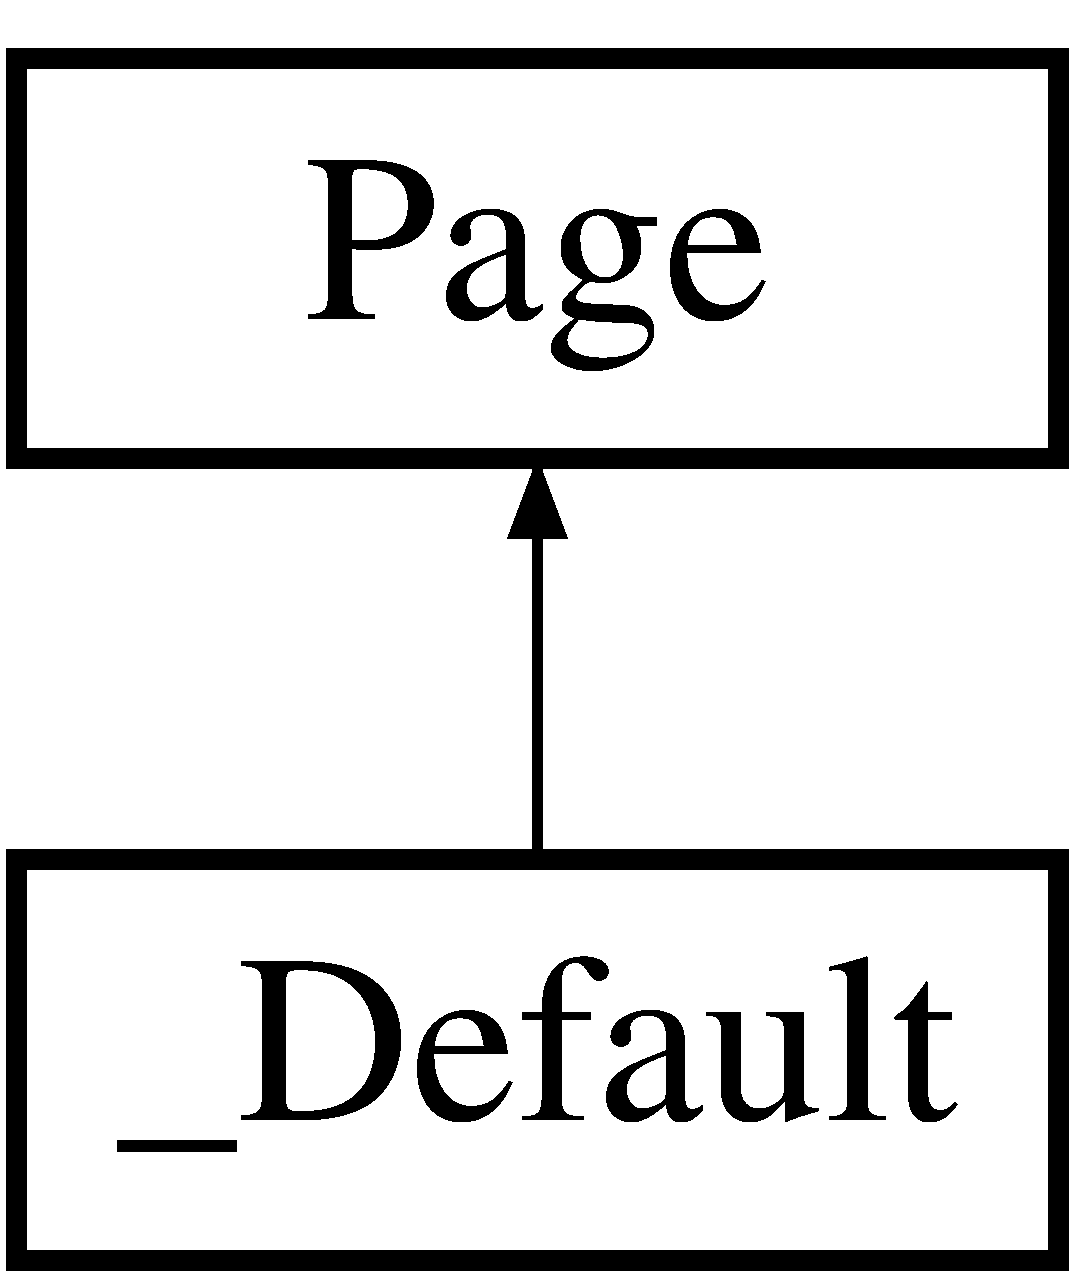
\includegraphics[height=2.000000cm]{class___default}
\end{center}
\end{figure}
\subsection*{Protected Member Functions}
\begin{DoxyCompactItemize}
\item 
\hypertarget{class___default_adacf7c92cb8d02f22ce02f0ceed897c1}{void {\bfseries Page\-\_\-\-Load} (object sender, Event\-Args e)}\label{class___default_adacf7c92cb8d02f22ce02f0ceed897c1}

\item 
\hypertarget{class___default_acf1cf3360aeecb29886ab98e0065144b}{void {\bfseries back\-\_\-\-Click} (object sender, Image\-Click\-Event\-Args e)}\label{class___default_acf1cf3360aeecb29886ab98e0065144b}

\item 
\hypertarget{class___default_a599b0fe5110ff03bca7be129c1f150a3}{void {\bfseries next\-\_\-\-Click} (object sender, Image\-Click\-Event\-Args e)}\label{class___default_a599b0fe5110ff03bca7be129c1f150a3}

\item 
\hypertarget{class___default_af1064f05babee44e874a165350cd0b9e}{void {\bfseries txtpage\-\_\-\-Text\-Changed} (object sender, Event\-Args e)}\label{class___default_af1064f05babee44e874a165350cd0b9e}

\end{DoxyCompactItemize}


\subsection{Detailed Description}


Definition at line 8 of file Default.\-aspx.\-cs.



The documentation for this class was generated from the following file\-:\begin{DoxyCompactItemize}
\item 
E\-:/\-Mint/\-Home care/\-Smart\-Home\-Care/Default.\-aspx.\-cs\end{DoxyCompactItemize}

\hypertarget{classadmincompose}{\section{admincompose Class Reference}
\label{classadmincompose}\index{admincompose@{admincompose}}
}
Inheritance diagram for admincompose\-:\begin{figure}[H]
\begin{center}
\leavevmode
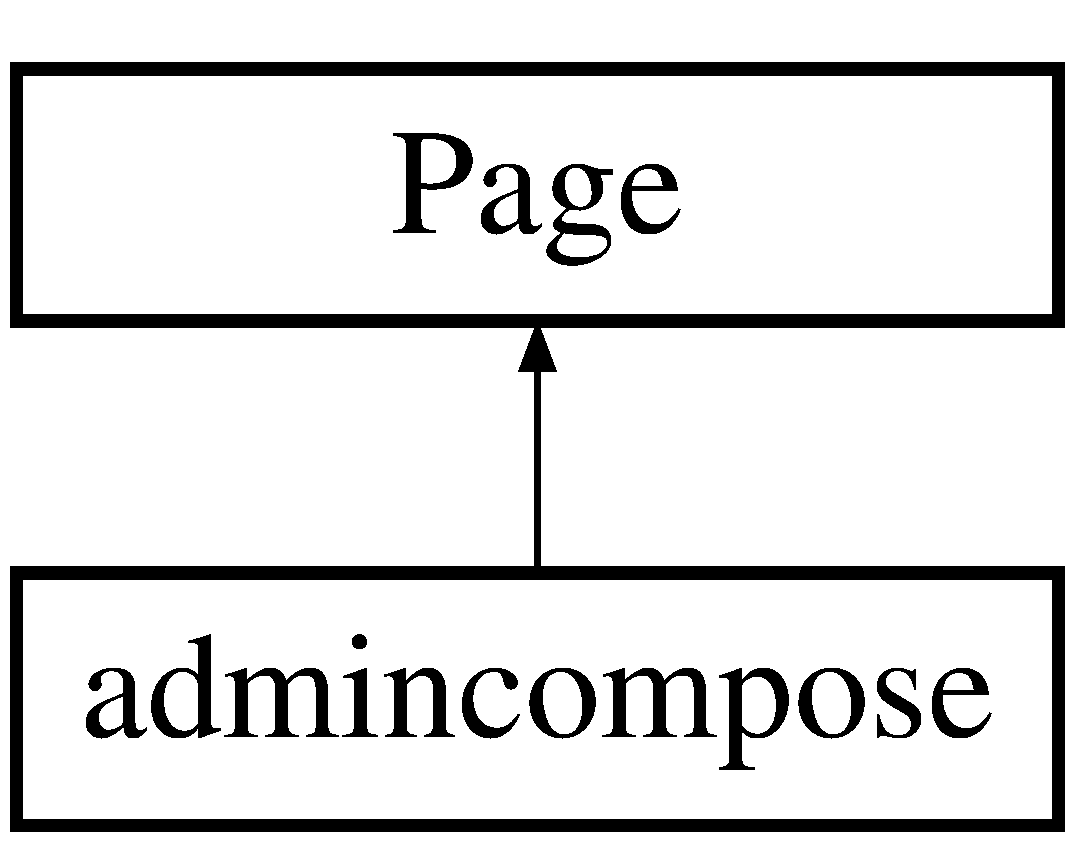
\includegraphics[height=2.000000cm]{classadmincompose}
\end{center}
\end{figure}
\subsection*{Static Public Member Functions}
\begin{DoxyCompactItemize}
\item 
\hypertarget{classadmincompose_a048a86e0c84363d80553d245266ebddc}{static object {\bfseries Send\-Mail\-To\-User} (object\mbox{[}$\,$\mbox{]} args)}\label{classadmincompose_a048a86e0c84363d80553d245266ebddc}

\end{DoxyCompactItemize}
\subsection*{Protected Member Functions}
\begin{DoxyCompactItemize}
\item 
\hypertarget{classadmincompose_a0b12819d930fd60d00069752e89333e1}{void {\bfseries Page\-\_\-\-Load} (object sender, Event\-Args e)}\label{classadmincompose_a0b12819d930fd60d00069752e89333e1}

\item 
void \hyperlink{classadmincompose_a887593d120b4d4c7f71fbd1c24ad6b03}{btn\-Send\-\_\-\-Click} (object sender, Event\-Args e)
\end{DoxyCompactItemize}


\subsection{Detailed Description}


Definition at line 9 of file admincompose.\-aspx.\-cs.



\subsection{Member Function Documentation}
\hypertarget{classadmincompose_a887593d120b4d4c7f71fbd1c24ad6b03}{\index{admincompose@{admincompose}!btn\-Send\-\_\-\-Click@{btn\-Send\-\_\-\-Click}}
\index{btn\-Send\-\_\-\-Click@{btn\-Send\-\_\-\-Click}!admincompose@{admincompose}}
\subsubsection[{btn\-Send\-\_\-\-Click}]{\setlength{\rightskip}{0pt plus 5cm}void admincompose.\-btn\-Send\-\_\-\-Click (
\begin{DoxyParamCaption}
\item[{object}]{sender, }
\item[{Event\-Args}]{e}
\end{DoxyParamCaption}
)\hspace{0.3cm}{\ttfamily [protected]}}}\label{classadmincompose_a887593d120b4d4c7f71fbd1c24ad6b03}
\mbox{[}Send\mbox{]} Send messages and redirect inbox.\-if no success -\/$>$ notification sent error 

Definition at line 55 of file admincompose.\-aspx.\-cs.



The documentation for this class was generated from the following file\-:\begin{DoxyCompactItemize}
\item 
E\-:/\-Mint/\-Home care/\-Smart\-Home\-Care/admincompose.\-aspx.\-cs\end{DoxyCompactItemize}

\hypertarget{classadminhelp}{\section{adminhelp Class Reference}
\label{classadminhelp}\index{adminhelp@{adminhelp}}
}
Inheritance diagram for adminhelp\-:\begin{figure}[H]
\begin{center}
\leavevmode
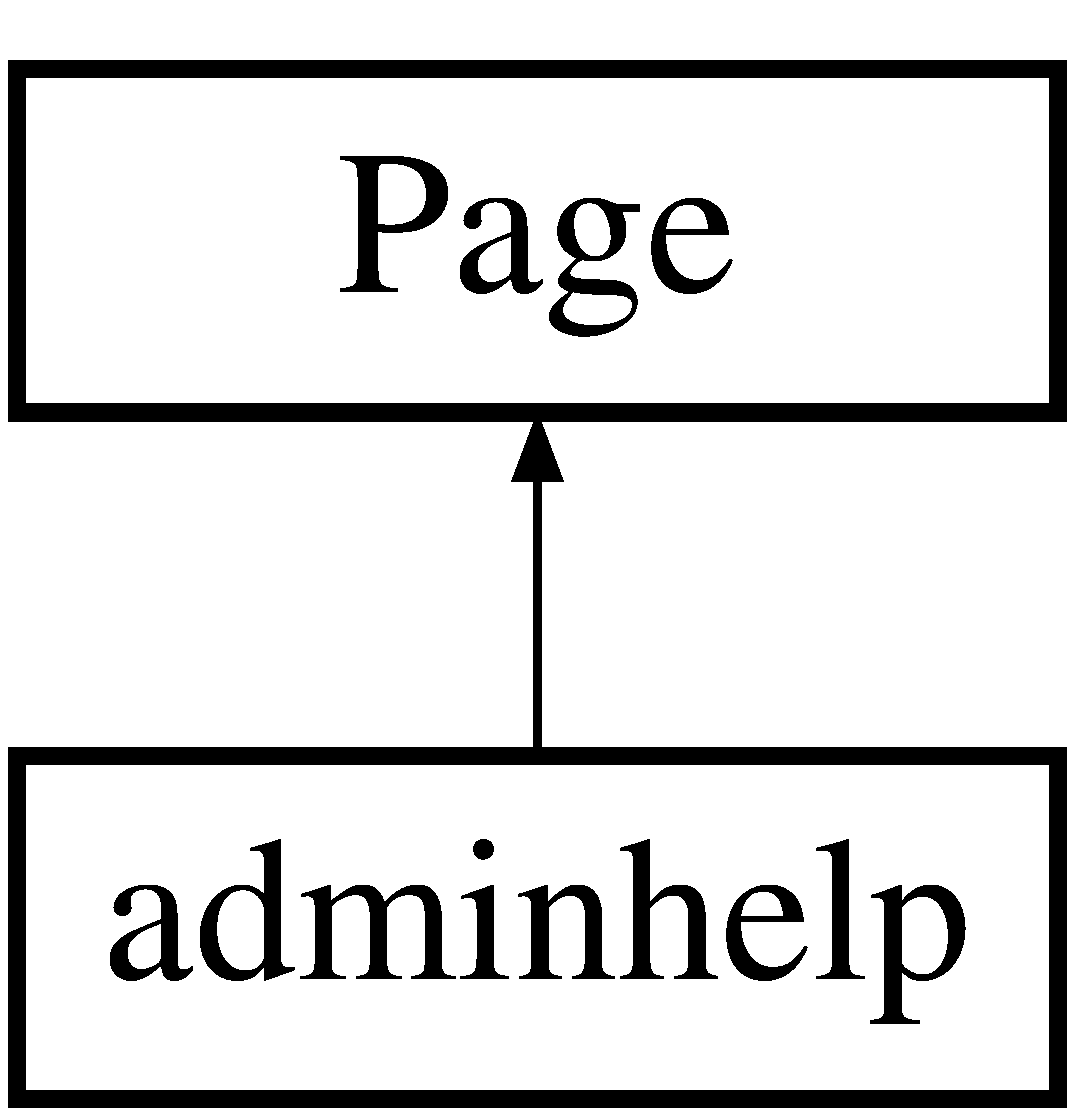
\includegraphics[height=2.000000cm]{classadminhelp}
\end{center}
\end{figure}
\subsection*{Protected Member Functions}
\begin{DoxyCompactItemize}
\item 
\hypertarget{classadminhelp_ae9508db86c07922a53c4f3f46e7ab27e}{void {\bfseries Page\-\_\-\-Load} (object sender, Event\-Args e)}\label{classadminhelp_ae9508db86c07922a53c4f3f46e7ab27e}

\end{DoxyCompactItemize}


\subsection{Detailed Description}


Definition at line 8 of file adminhelp.\-aspx.\-cs.



The documentation for this class was generated from the following file\-:\begin{DoxyCompactItemize}
\item 
E\-:/\-Mint/\-Home care/\-Smart\-Home\-Care/adminhelp.\-aspx.\-cs\end{DoxyCompactItemize}

\hypertarget{classadmininbox}{\section{admininbox Class Reference}
\label{classadmininbox}\index{admininbox@{admininbox}}
}
Inheritance diagram for admininbox\-:\begin{figure}[H]
\begin{center}
\leavevmode
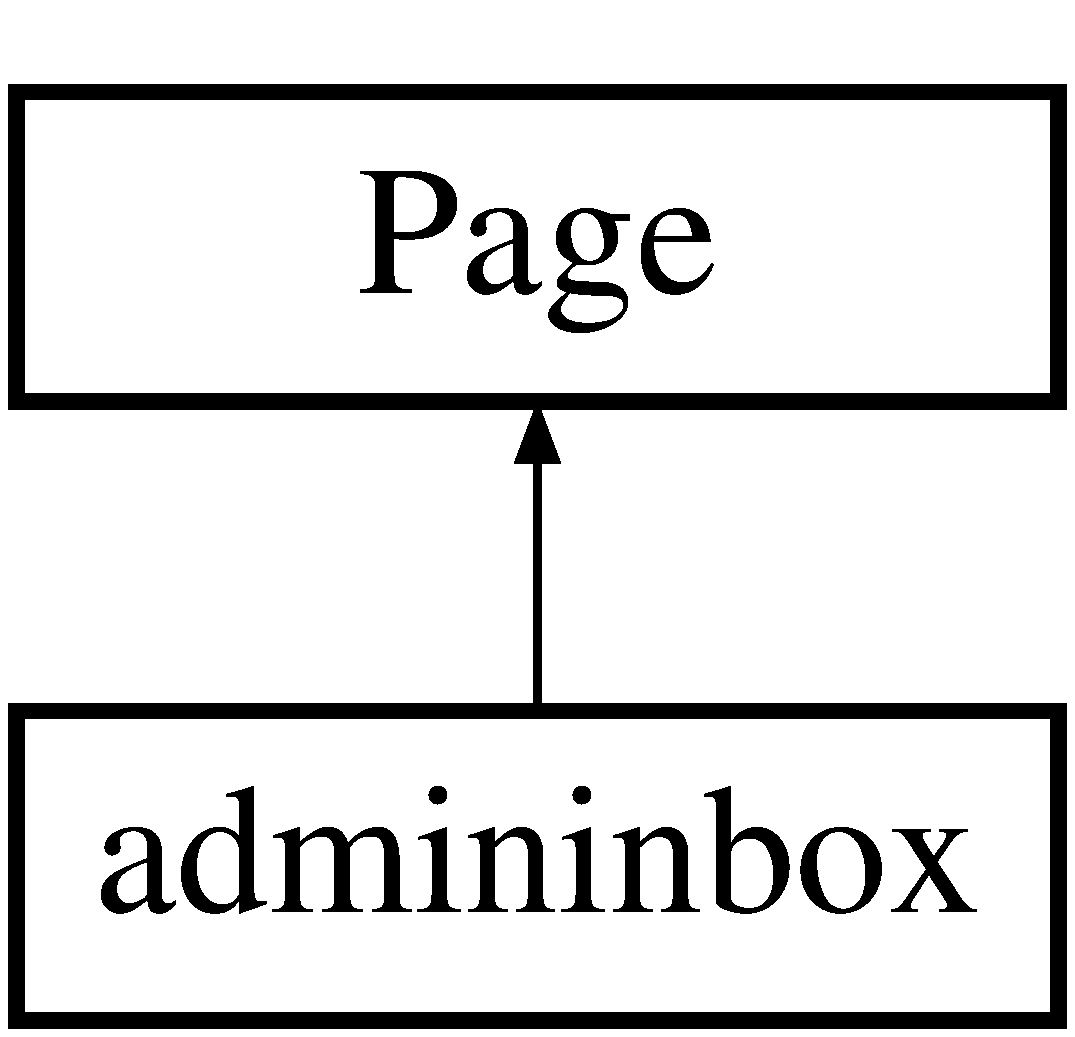
\includegraphics[height=2.000000cm]{classadmininbox}
\end{center}
\end{figure}
\subsection*{Static Public Member Functions}
\begin{DoxyCompactItemize}
\item 
\hypertarget{classadmininbox_a60a1a00372ec1d3d7de257c173db53d3}{static object {\bfseries Read\-Message} (int id)}\label{classadmininbox_a60a1a00372ec1d3d7de257c173db53d3}

\item 
\hypertarget{classadmininbox_afc770337f86eb257eadf046d8082016d}{static object {\bfseries Delete\-Message} (object args)}\label{classadmininbox_afc770337f86eb257eadf046d8082016d}

\end{DoxyCompactItemize}
\subsection*{Protected Member Functions}
\begin{DoxyCompactItemize}
\item 
\hypertarget{classadmininbox_a8affc3f6a49da6324782959b814ad7d3}{void {\bfseries Page\-\_\-\-Load} (object sender, Event\-Args e)}\label{classadmininbox_a8affc3f6a49da6324782959b814ad7d3}

\item 
void \hyperlink{classadmininbox_aeba572f2e0c6f40050937bc6b3a029dc}{btndelete\-\_\-\-Click} (object sender, Event\-Args e)
\item 
\hypertarget{classadmininbox_a1c338121a7e66023c10108b7a9d216f7}{void {\bfseries Link\-Button2\-\_\-\-Click} (object sender, Event\-Args e)}\label{classadmininbox_a1c338121a7e66023c10108b7a9d216f7}

\item 
\hypertarget{classadmininbox_add101808519d90270943f2353f11b6c2}{void {\bfseries lb\-Pre\-\_\-\-Click} (object sender, Event\-Args e)}\label{classadmininbox_add101808519d90270943f2353f11b6c2}

\end{DoxyCompactItemize}


\subsection{Detailed Description}


Definition at line 8 of file admininbox.\-aspx.\-cs.



\subsection{Member Function Documentation}
\hypertarget{classadmininbox_aeba572f2e0c6f40050937bc6b3a029dc}{\index{admininbox@{admininbox}!btndelete\-\_\-\-Click@{btndelete\-\_\-\-Click}}
\index{btndelete\-\_\-\-Click@{btndelete\-\_\-\-Click}!admininbox@{admininbox}}
\subsubsection[{btndelete\-\_\-\-Click}]{\setlength{\rightskip}{0pt plus 5cm}void admininbox.\-btndelete\-\_\-\-Click (
\begin{DoxyParamCaption}
\item[{object}]{sender, }
\item[{Event\-Args}]{e}
\end{DoxyParamCaption}
)\hspace{0.3cm}{\ttfamily [protected]}}}\label{classadmininbox_aeba572f2e0c6f40050937bc6b3a029dc}
\mbox{[}Delete\mbox{]} delete message checked. 

Definition at line 55 of file admininbox.\-aspx.\-cs.



The documentation for this class was generated from the following file\-:\begin{DoxyCompactItemize}
\item 
E\-:/\-Mint/\-Home care/\-Smart\-Home\-Care/admininbox.\-aspx.\-cs\end{DoxyCompactItemize}

\hypertarget{classadminmyaccount}{\section{adminmyaccount Class Reference}
\label{classadminmyaccount}\index{adminmyaccount@{adminmyaccount}}
}
Inheritance diagram for adminmyaccount\-:\begin{figure}[H]
\begin{center}
\leavevmode
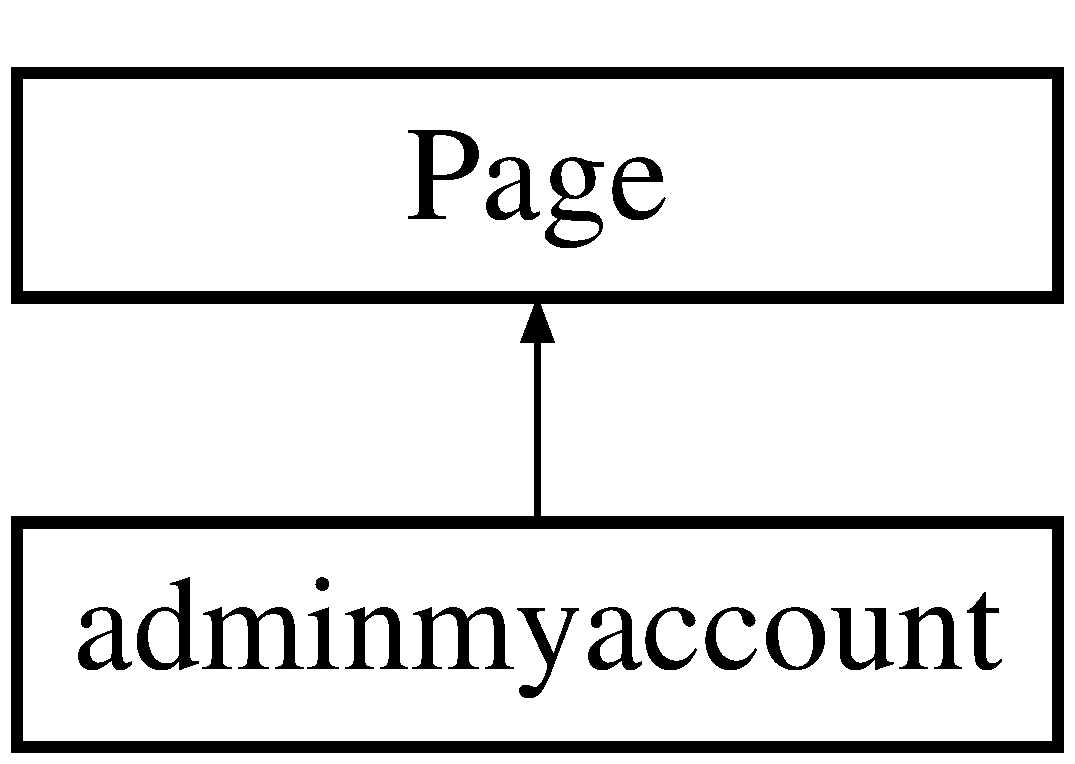
\includegraphics[height=2.000000cm]{classadminmyaccount}
\end{center}
\end{figure}
\subsection*{Protected Member Functions}
\begin{DoxyCompactItemize}
\item 
\hypertarget{classadminmyaccount_af3bc2358b578da42fdcde6e35d83d807}{void {\bfseries Page\-\_\-\-Load} (object sender, Event\-Args e)}\label{classadminmyaccount_af3bc2358b578da42fdcde6e35d83d807}

\item 
\hypertarget{classadminmyaccount_ab1ceb89cf05222cf5f61eb9c9e6f460b}{void {\bfseries btnedit\-\_\-\-Click} (object sender, Event\-Args e)}\label{classadminmyaccount_ab1ceb89cf05222cf5f61eb9c9e6f460b}

\item 
\hypertarget{classadminmyaccount_af54811c66f1b8f8bbfe164c6c6ad8ed2}{void {\bfseries btnsave\-\_\-\-Click} (object sender, Event\-Args e)}\label{classadminmyaccount_af54811c66f1b8f8bbfe164c6c6ad8ed2}

\item 
\hypertarget{classadminmyaccount_aebf1f3c30c02c4ed5c4f5068c8627299}{void {\bfseries btncancel\-\_\-\-Click} (object sender, Event\-Args e)}\label{classadminmyaccount_aebf1f3c30c02c4ed5c4f5068c8627299}

\end{DoxyCompactItemize}


\subsection{Detailed Description}


Definition at line 8 of file adminmyaccount.\-aspx.\-cs.



The documentation for this class was generated from the following file\-:\begin{DoxyCompactItemize}
\item 
E\-:/\-Mint/\-Home care/\-Smart\-Home\-Care/adminmyaccount.\-aspx.\-cs\end{DoxyCompactItemize}

\hypertarget{classadminpaybill__detail}{\section{adminpaybill\-\_\-detail Class Reference}
\label{classadminpaybill__detail}\index{adminpaybill\-\_\-detail@{adminpaybill\-\_\-detail}}
}
Inheritance diagram for adminpaybill\-\_\-detail\-:\begin{figure}[H]
\begin{center}
\leavevmode
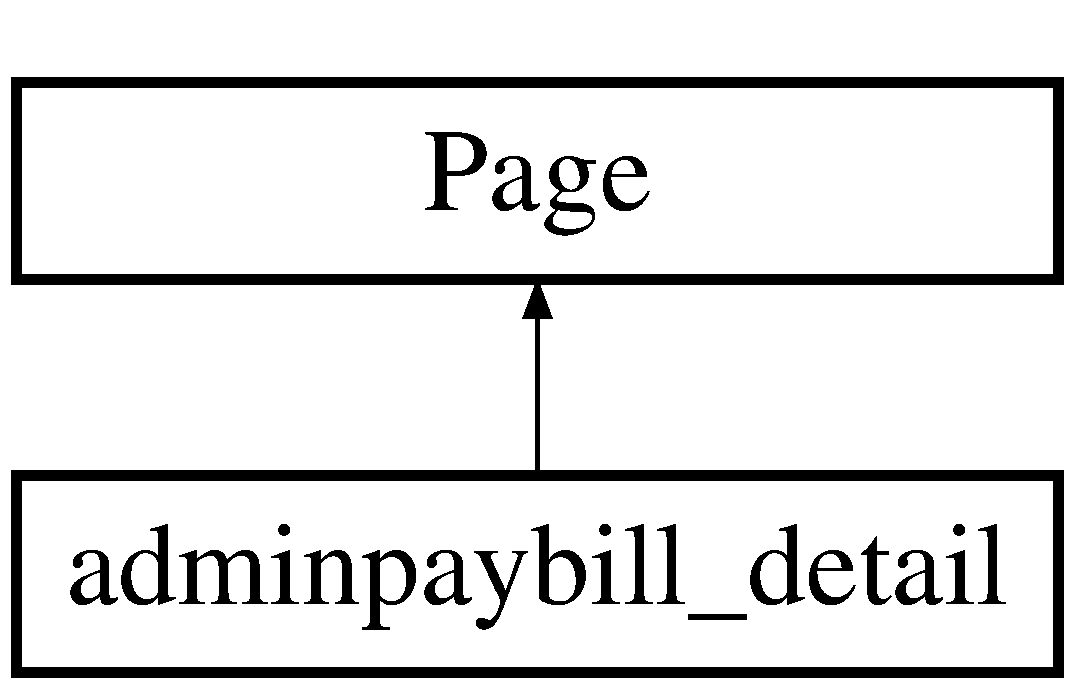
\includegraphics[height=2.000000cm]{classadminpaybill__detail}
\end{center}
\end{figure}
\subsection*{Protected Member Functions}
\begin{DoxyCompactItemize}
\item 
\hypertarget{classadminpaybill__detail_acf372407b84cc070e8fd6efb18cbbcbc}{void {\bfseries Page\-\_\-\-Load} (object sender, Event\-Args e)}\label{classadminpaybill__detail_acf372407b84cc070e8fd6efb18cbbcbc}

\item 
\hypertarget{classadminpaybill__detail_ab2fb914876175622f3f461bcd69003c2}{void {\bfseries chk\-Paybill\-\_\-\-Checked\-Changed} (object sender, Event\-Args e)}\label{classadminpaybill__detail_ab2fb914876175622f3f461bcd69003c2}

\end{DoxyCompactItemize}


\subsection{Detailed Description}


Definition at line 8 of file adminpaybill\-\_\-detail.\-aspx.\-cs.



The documentation for this class was generated from the following file\-:\begin{DoxyCompactItemize}
\item 
E\-:/\-Mint/\-Home care/\-Smart\-Home\-Care/adminpaybill\-\_\-detail.\-aspx.\-cs\end{DoxyCompactItemize}

\hypertarget{classadminreportstatistics}{\section{adminreportstatistics Class Reference}
\label{classadminreportstatistics}\index{adminreportstatistics@{adminreportstatistics}}
}
Inheritance diagram for adminreportstatistics\-:\begin{figure}[H]
\begin{center}
\leavevmode
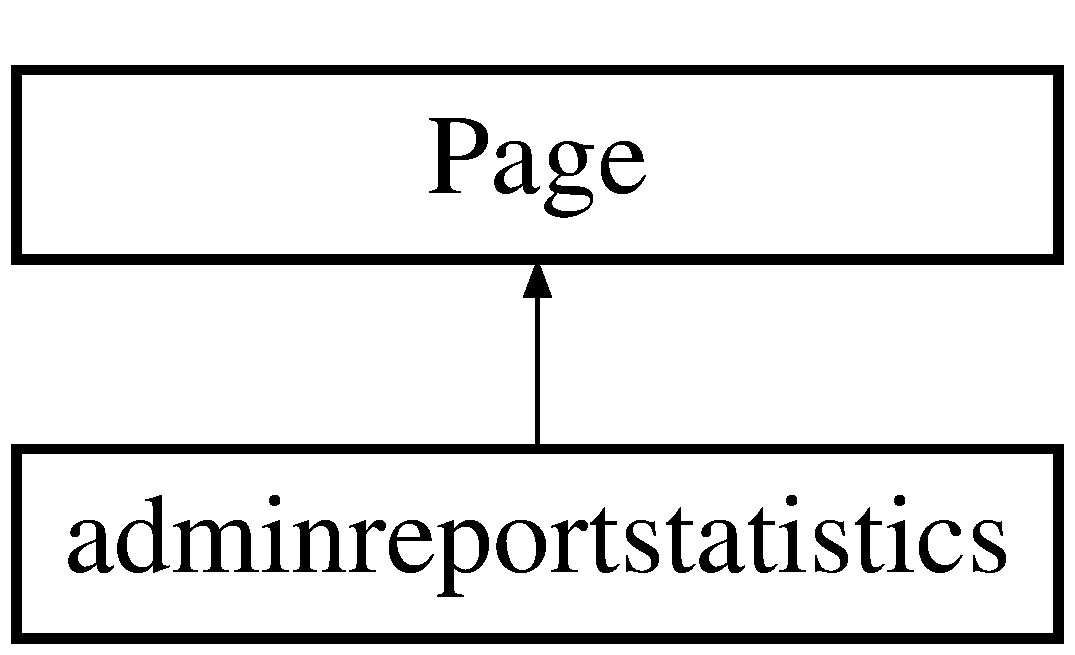
\includegraphics[height=2.000000cm]{classadminreportstatistics}
\end{center}
\end{figure}
\subsection*{Protected Member Functions}
\begin{DoxyCompactItemize}
\item 
\hypertarget{classadminreportstatistics_a51b830b544b59599b892de52a1d8f137}{void {\bfseries Page\-\_\-\-Load} (object sender, Event\-Args e)}\label{classadminreportstatistics_a51b830b544b59599b892de52a1d8f137}

\end{DoxyCompactItemize}


\subsection{Detailed Description}


Definition at line 8 of file adminreportstatistics.\-aspx.\-cs.



The documentation for this class was generated from the following file\-:\begin{DoxyCompactItemize}
\item 
E\-:/\-Mint/\-Home care/\-Smart\-Home\-Care/adminreportstatistics.\-aspx.\-cs\end{DoxyCompactItemize}

\hypertarget{classadminsentmessages}{\section{adminsentmessages Class Reference}
\label{classadminsentmessages}\index{adminsentmessages@{adminsentmessages}}
}
Inheritance diagram for adminsentmessages\-:\begin{figure}[H]
\begin{center}
\leavevmode
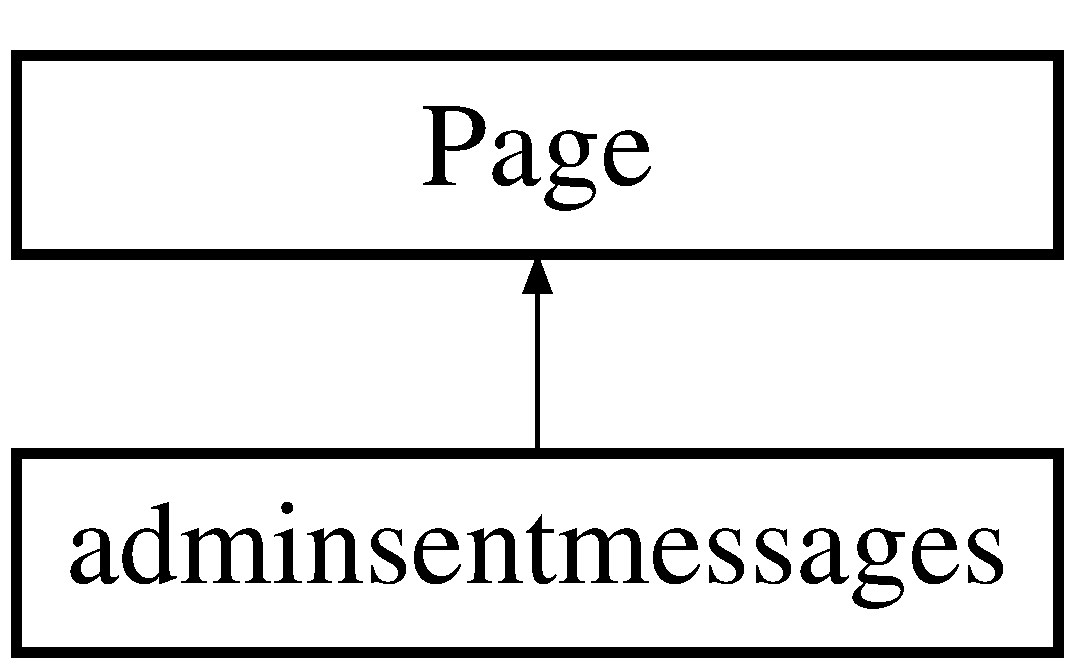
\includegraphics[height=2.000000cm]{classadminsentmessages}
\end{center}
\end{figure}
\subsection*{Static Public Member Functions}
\begin{DoxyCompactItemize}
\item 
\hypertarget{classadminsentmessages_ae3e3185b9751f6aef6fe832c6995d17f}{static object {\bfseries Read\-Message} (int id)}\label{classadminsentmessages_ae3e3185b9751f6aef6fe832c6995d17f}

\item 
\hypertarget{classadminsentmessages_a970719d48af108e5e98e8bb6ed61d0c0}{static object {\bfseries Delete\-Message} (object args)}\label{classadminsentmessages_a970719d48af108e5e98e8bb6ed61d0c0}

\item 
\hypertarget{classadminsentmessages_aea658fbdfd1eee4bfa4cea2a42735490}{static object {\bfseries Empty\-Trash\-Service} (object args)}\label{classadminsentmessages_aea658fbdfd1eee4bfa4cea2a42735490}

\end{DoxyCompactItemize}
\subsection*{Protected Member Functions}
\begin{DoxyCompactItemize}
\item 
\hypertarget{classadminsentmessages_a002928c0327e8c487949d9e6207b9f2f}{void {\bfseries Page\-\_\-\-Load} (object sender, Event\-Args e)}\label{classadminsentmessages_a002928c0327e8c487949d9e6207b9f2f}

\item 
\hypertarget{classadminsentmessages_a48aac92fad16543e878e38514956d8a6}{void {\bfseries btndelete\-\_\-\-Click} (object sender, Event\-Args e)}\label{classadminsentmessages_a48aac92fad16543e878e38514956d8a6}

\item 
\hypertarget{classadminsentmessages_ad2efc9592870c548d36ef5ba6dd52fd7}{void {\bfseries Link\-Button2\-\_\-\-Click} (object sender, Event\-Args e)}\label{classadminsentmessages_ad2efc9592870c548d36ef5ba6dd52fd7}

\item 
\hypertarget{classadminsentmessages_a2818cf63646056dacf6cc9818174a61d}{void {\bfseries lb\-Pre\-\_\-\-Click} (object sender, Event\-Args e)}\label{classadminsentmessages_a2818cf63646056dacf6cc9818174a61d}

\item 
\hypertarget{classadminsentmessages_a00bf6f729f8e2dcee18a46717e838520}{void {\bfseries btn\-Empty\-\_\-\-Click} (object sender, Event\-Args e)}\label{classadminsentmessages_a00bf6f729f8e2dcee18a46717e838520}

\end{DoxyCompactItemize}


\subsection{Detailed Description}


Definition at line 8 of file adminsentmessages.\-aspx.\-cs.



The documentation for this class was generated from the following file\-:\begin{DoxyCompactItemize}
\item 
E\-:/\-Mint/\-Home care/\-Smart\-Home\-Care/adminsentmessages.\-aspx.\-cs\end{DoxyCompactItemize}

\hypertarget{classadminsitemap}{\section{adminsitemap Class Reference}
\label{classadminsitemap}\index{adminsitemap@{adminsitemap}}
}
Inheritance diagram for adminsitemap\-:\begin{figure}[H]
\begin{center}
\leavevmode
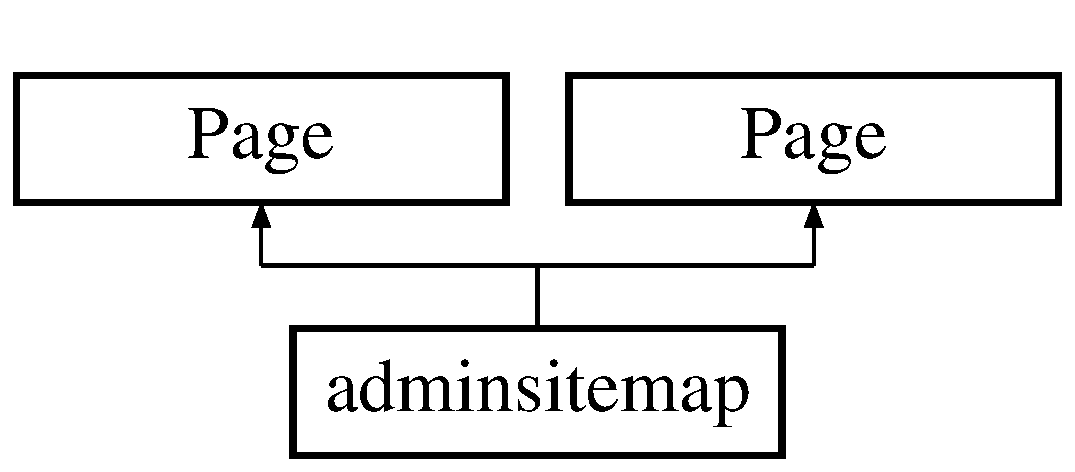
\includegraphics[height=2.000000cm]{classadminsitemap}
\end{center}
\end{figure}
\subsection*{Protected Member Functions}
\begin{DoxyCompactItemize}
\item 
\hypertarget{classadminsitemap_a124c8997fd52c92c75866852a1586fb3}{void {\bfseries Page\-\_\-\-Load} (object sender, Event\-Args e)}\label{classadminsitemap_a124c8997fd52c92c75866852a1586fb3}

\item 
\hypertarget{classadminsitemap_a124c8997fd52c92c75866852a1586fb3}{void {\bfseries Page\-\_\-\-Load} (object sender, Event\-Args e)}\label{classadminsitemap_a124c8997fd52c92c75866852a1586fb3}

\end{DoxyCompactItemize}


\subsection{Detailed Description}


Definition at line 8 of file adminsitemap.\-aspx.\-cs.



The documentation for this class was generated from the following files\-:\begin{DoxyCompactItemize}
\item 
E\-:/\-Mint/\-Home care/\-Smart\-Home\-Care/adminsitemap.\-aspx.\-cs\item 
E\-:/\-Mint/\-Home care/\-Smart\-Home\-Care/x\-\_\-adminsitemap.\-aspx.\-cs\end{DoxyCompactItemize}

\hypertarget{classadminsynclogs}{\section{adminsynclogs Class Reference}
\label{classadminsynclogs}\index{adminsynclogs@{adminsynclogs}}
}
Inheritance diagram for adminsynclogs\-:\begin{figure}[H]
\begin{center}
\leavevmode
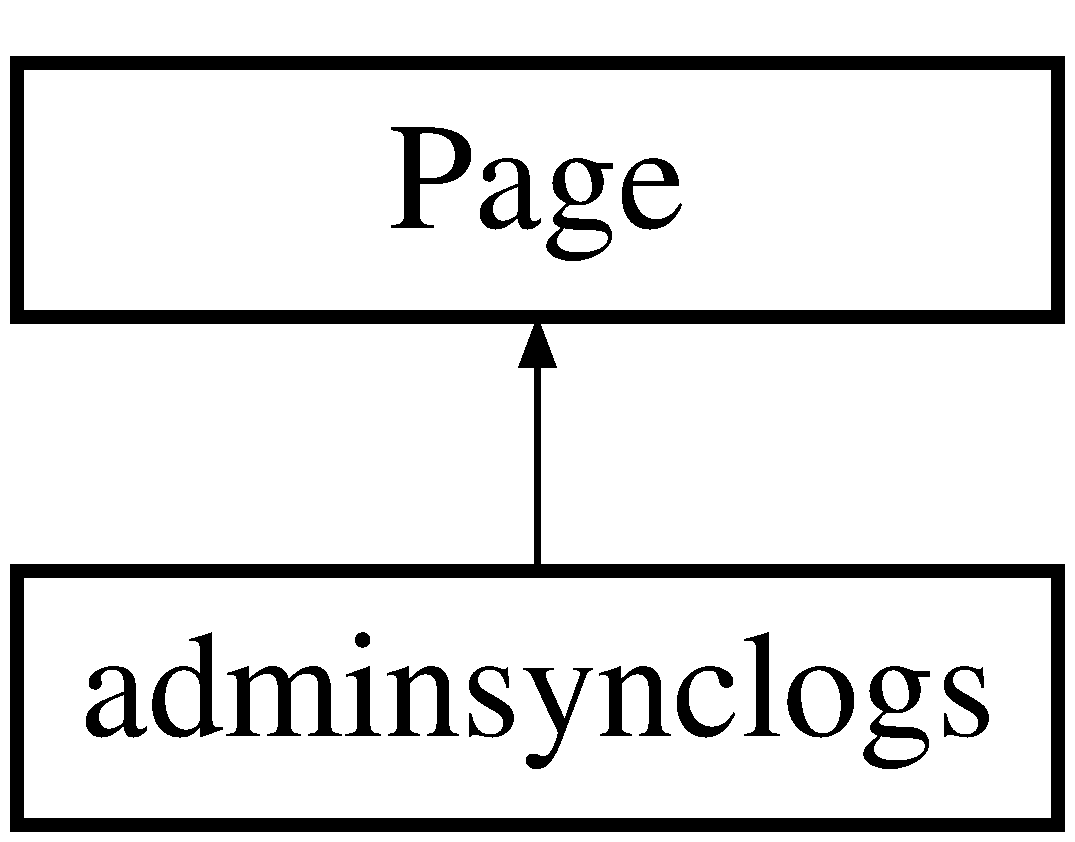
\includegraphics[height=2.000000cm]{classadminsynclogs}
\end{center}
\end{figure}
\subsection*{Protected Member Functions}
\begin{DoxyCompactItemize}
\item 
\hypertarget{classadminsynclogs_a5d2623b0a8c872c7bbe68dbaab7ee45b}{void {\bfseries Page\-\_\-\-Load} (object sender, Event\-Args e)}\label{classadminsynclogs_a5d2623b0a8c872c7bbe68dbaab7ee45b}

\end{DoxyCompactItemize}


\subsection{Detailed Description}


Definition at line 8 of file adminsynclogs.\-aspx.\-cs.



The documentation for this class was generated from the following file\-:\begin{DoxyCompactItemize}
\item 
E\-:/\-Mint/\-Home care/\-Smart\-Home\-Care/adminsynclogs.\-aspx.\-cs\end{DoxyCompactItemize}

\hypertarget{classadmintrash}{\section{admintrash Class Reference}
\label{classadmintrash}\index{admintrash@{admintrash}}
}
Inheritance diagram for admintrash\-:\begin{figure}[H]
\begin{center}
\leavevmode
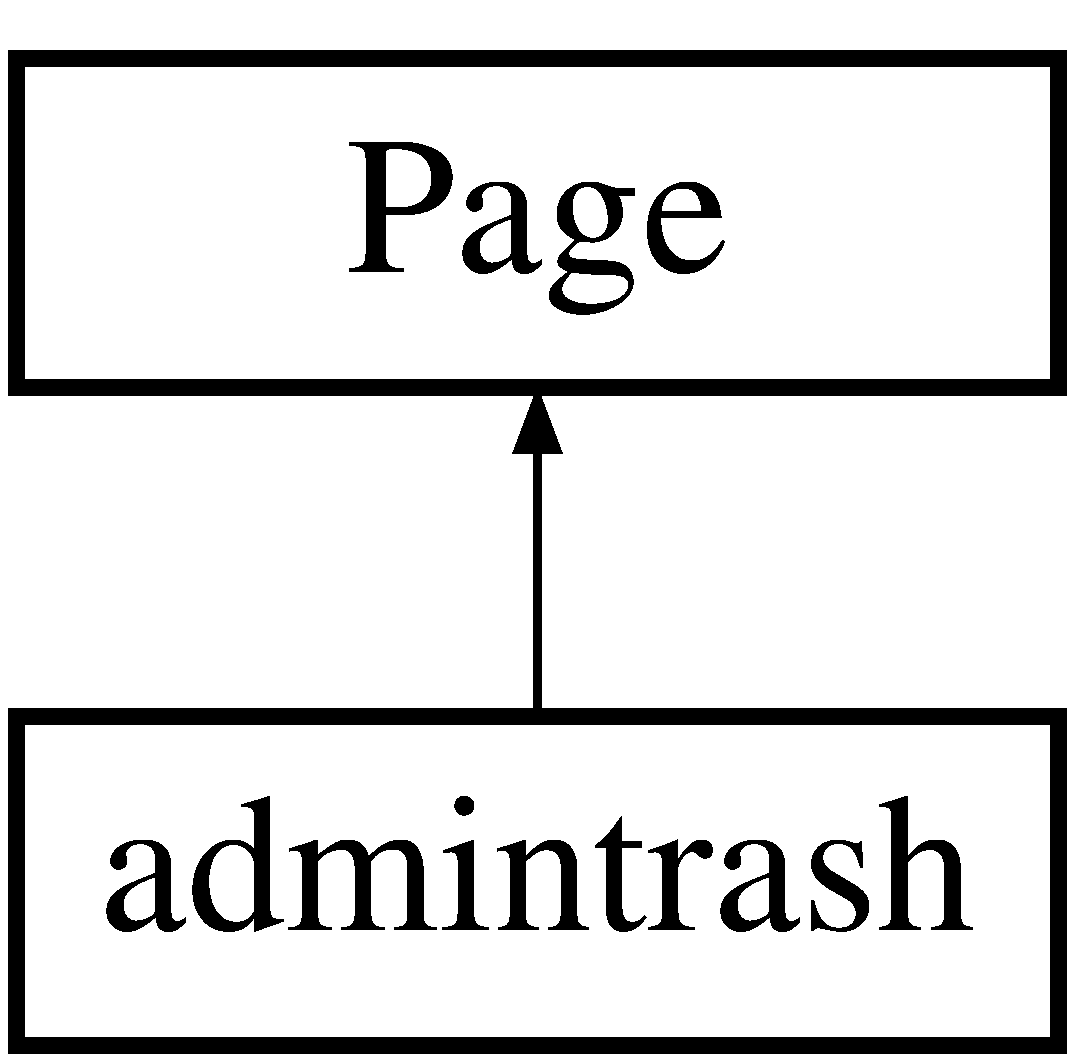
\includegraphics[height=2.000000cm]{classadmintrash}
\end{center}
\end{figure}
\subsection*{Static Public Member Functions}
\begin{DoxyCompactItemize}
\item 
\hypertarget{classadmintrash_a4faca7d4ece5b3733901e6017008485c}{static object {\bfseries Read\-Message} (int id)}\label{classadmintrash_a4faca7d4ece5b3733901e6017008485c}

\item 
\hypertarget{classadmintrash_a3d85f4a3152c90727a604892b3ae2dd2}{static object {\bfseries Delete\-Message} (object args)}\label{classadmintrash_a3d85f4a3152c90727a604892b3ae2dd2}

\item 
\hypertarget{classadmintrash_a599156bd78b8001b73b094815970e88a}{static object {\bfseries Empty\-Trash\-Service} (object args)}\label{classadmintrash_a599156bd78b8001b73b094815970e88a}

\end{DoxyCompactItemize}
\subsection*{Public Attributes}
\begin{DoxyCompactItemize}
\item 
\hypertarget{classadmintrash_ac2f0c4979386918142771eabf5b0f727}{string {\bfseries Ids} = \char`\"{}\char`\"{}}\label{classadmintrash_ac2f0c4979386918142771eabf5b0f727}

\end{DoxyCompactItemize}
\subsection*{Protected Member Functions}
\begin{DoxyCompactItemize}
\item 
\hypertarget{classadmintrash_a9b87503d8a1465d91d18833f957fea90}{void {\bfseries Page\-\_\-\-Load} (object sender, Event\-Args e)}\label{classadmintrash_a9b87503d8a1465d91d18833f957fea90}

\item 
void \hyperlink{classadmintrash_a331ac56cdc0d25dc4e3d25faa8a16bc3}{btn\-Delete\-\_\-\-Click} (object sender, Event\-Args e)
\item 
\hypertarget{classadmintrash_a5b7b7a915dabf249d1545b5ee00c7afc}{void {\bfseries Link\-Button2\-\_\-\-Click} (object sender, Event\-Args e)}\label{classadmintrash_a5b7b7a915dabf249d1545b5ee00c7afc}

\item 
\hypertarget{classadmintrash_ab65f2ef3434c2a208a02ae1468c2ae78}{void {\bfseries lb\-Pre\-\_\-\-Click} (object sender, Event\-Args e)}\label{classadmintrash_ab65f2ef3434c2a208a02ae1468c2ae78}

\end{DoxyCompactItemize}


\subsection{Detailed Description}


Definition at line 8 of file admintrash.\-aspx.\-cs.



\subsection{Member Function Documentation}
\hypertarget{classadmintrash_a331ac56cdc0d25dc4e3d25faa8a16bc3}{\index{admintrash@{admintrash}!btn\-Delete\-\_\-\-Click@{btn\-Delete\-\_\-\-Click}}
\index{btn\-Delete\-\_\-\-Click@{btn\-Delete\-\_\-\-Click}!admintrash@{admintrash}}
\subsubsection[{btn\-Delete\-\_\-\-Click}]{\setlength{\rightskip}{0pt plus 5cm}void admintrash.\-btn\-Delete\-\_\-\-Click (
\begin{DoxyParamCaption}
\item[{object}]{sender, }
\item[{Event\-Args}]{e}
\end{DoxyParamCaption}
)\hspace{0.3cm}{\ttfamily [protected]}}}\label{classadmintrash_a331ac56cdc0d25dc4e3d25faa8a16bc3}
\mbox{[}Delete\mbox{]} delete message trash. 

Definition at line 89 of file admintrash.\-aspx.\-cs.



The documentation for this class was generated from the following file\-:\begin{DoxyCompactItemize}
\item 
E\-:/\-Mint/\-Home care/\-Smart\-Home\-Care/admintrash.\-aspx.\-cs\end{DoxyCompactItemize}

\hypertarget{classadminusermanagement}{\section{adminusermanagement Class Reference}
\label{classadminusermanagement}\index{adminusermanagement@{adminusermanagement}}
}
Inheritance diagram for adminusermanagement\-:\begin{figure}[H]
\begin{center}
\leavevmode
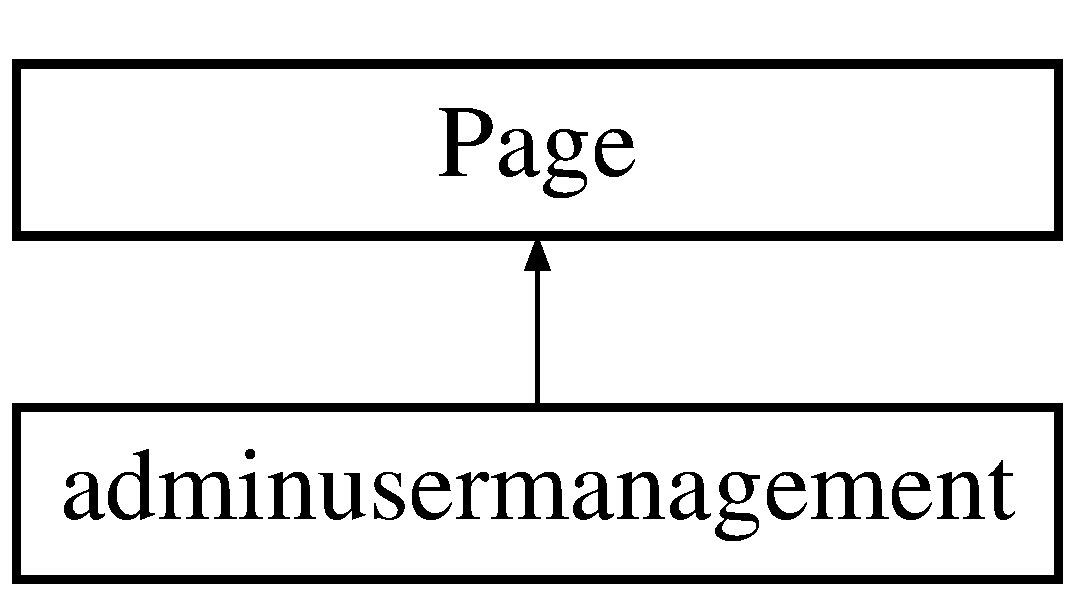
\includegraphics[height=2.000000cm]{classadminusermanagement}
\end{center}
\end{figure}
\subsection*{Protected Member Functions}
\begin{DoxyCompactItemize}
\item 
\hypertarget{classadminusermanagement_a517412da8a8db5bf157577fb071e7a49}{void {\bfseries Page\-\_\-\-Load} (object sender, Event\-Args e)}\label{classadminusermanagement_a517412da8a8db5bf157577fb071e7a49}

\item 
\hypertarget{classadminusermanagement_ae2bf386505932b34e197e30355135a6a}{void {\bfseries btnactive\-\_\-\-Click} (object sender, Event\-Args e)}\label{classadminusermanagement_ae2bf386505932b34e197e30355135a6a}

\item 
\hypertarget{classadminusermanagement_ad5d45dcf72259853a1c5ce0d5148d831}{void {\bfseries btndeactive\-\_\-\-Click} (object sender, Event\-Args e)}\label{classadminusermanagement_ad5d45dcf72259853a1c5ce0d5148d831}

\item 
\hypertarget{classadminusermanagement_aaf1a3d6b619f4a11db8b4a56ba7b41b1}{void {\bfseries grdusermanagement\-\_\-\-Page\-Index\-Changing} (object sender, Grid\-View\-Page\-Event\-Args e)}\label{classadminusermanagement_aaf1a3d6b619f4a11db8b4a56ba7b41b1}

\item 
\hypertarget{classadminusermanagement_ab8b2fb96a95adc5b0274178179b511cc}{void {\bfseries btnfilter\-\_\-\-Click} (object sender, Event\-Args e)}\label{classadminusermanagement_ab8b2fb96a95adc5b0274178179b511cc}

\end{DoxyCompactItemize}


\subsection{Detailed Description}


Definition at line 9 of file adminusermanagement.\-aspx.\-cs.



The documentation for this class was generated from the following file\-:\begin{DoxyCompactItemize}
\item 
E\-:/\-Mint/\-Home care/\-Smart\-Home\-Care/adminusermanagement.\-aspx.\-cs\end{DoxyCompactItemize}

\hypertarget{classadminusermanagement__details}{\section{adminusermanagement\-\_\-details Class Reference}
\label{classadminusermanagement__details}\index{adminusermanagement\-\_\-details@{adminusermanagement\-\_\-details}}
}
Inheritance diagram for adminusermanagement\-\_\-details\-:\begin{figure}[H]
\begin{center}
\leavevmode
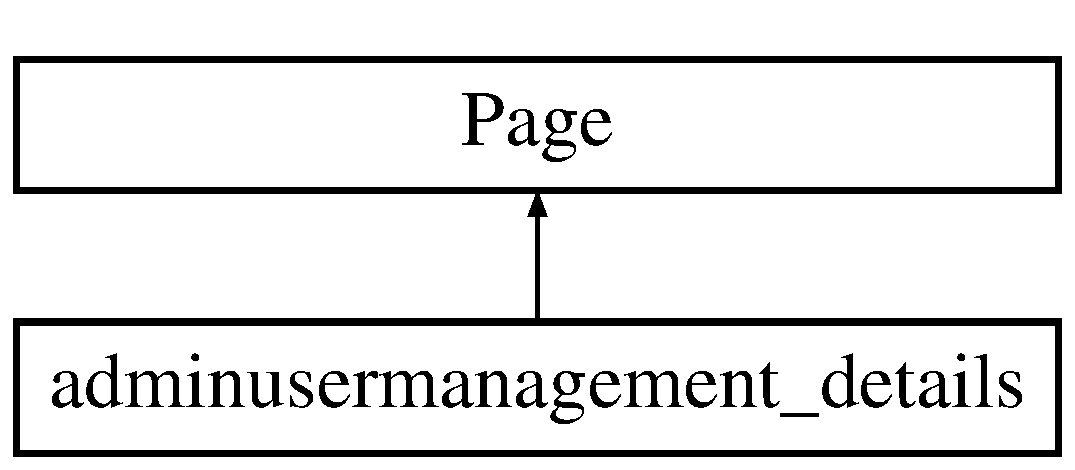
\includegraphics[height=2.000000cm]{classadminusermanagement__details}
\end{center}
\end{figure}
\subsection*{Protected Member Functions}
\begin{DoxyCompactItemize}
\item 
\hypertarget{classadminusermanagement__details_a063fdab8b5231ee5413de3f8e4833907}{void {\bfseries Page\-\_\-\-Load} (object sender, Event\-Args e)}\label{classadminusermanagement__details_a063fdab8b5231ee5413de3f8e4833907}

\item 
\hypertarget{classadminusermanagement__details_ae156604de3f7c4ae0c2c5feb1bfb22c0}{void {\bfseries btneditoverview\-\_\-\-Click} (object sender, Event\-Args e)}\label{classadminusermanagement__details_ae156604de3f7c4ae0c2c5feb1bfb22c0}

\item 
\hypertarget{classadminusermanagement__details_a2552ef32ed38e4a1b41e90eeaeb07bff}{void {\bfseries btnsaveoverview\-\_\-\-Click} (object sender, Event\-Args e)}\label{classadminusermanagement__details_a2552ef32ed38e4a1b41e90eeaeb07bff}

\item 
\hypertarget{classadminusermanagement__details_ac9e0ff2b7b4d5953c891d78951ceef4e}{void {\bfseries btncanceloverview\-\_\-\-Click} (object sender, Event\-Args e)}\label{classadminusermanagement__details_ac9e0ff2b7b4d5953c891d78951ceef4e}

\item 
\hypertarget{classadminusermanagement__details_a2c4f51a533078554fe5128848b70bf0e}{void {\bfseries btneditprofile\-\_\-\-Click} (object sender, Event\-Args e)}\label{classadminusermanagement__details_a2c4f51a533078554fe5128848b70bf0e}

\item 
\hypertarget{classadminusermanagement__details_a6f2ee46fc7c65b4aecbdc8f5203bd530}{void {\bfseries btnsaveprofile\-\_\-\-Click} (object sender, Event\-Args e)}\label{classadminusermanagement__details_a6f2ee46fc7c65b4aecbdc8f5203bd530}

\item 
\hypertarget{classadminusermanagement__details_a3cfca8e7c4922d0bd51abf93b11973ef}{void {\bfseries btncancelprofile\-\_\-\-Click} (object sender, Event\-Args e)}\label{classadminusermanagement__details_a3cfca8e7c4922d0bd51abf93b11973ef}

\item 
\hypertarget{classadminusermanagement__details_a773d4760a9cb59830fcc1ab78951ecfd}{void {\bfseries btnsavepreferentces\-\_\-\-Click} (object sender, Event\-Args e)}\label{classadminusermanagement__details_a773d4760a9cb59830fcc1ab78951ecfd}

\item 
\hypertarget{classadminusermanagement__details_a56eac8232a9166afe8b3c93bab5ae643}{void {\bfseries ddlcountry\-\_\-\-Selected\-Index\-Changed} (object sender, Event\-Args e)}\label{classadminusermanagement__details_a56eac8232a9166afe8b3c93bab5ae643}

\item 
\hypertarget{classadminusermanagement__details_aa7986204975ebb18b38360880c2af6ff}{void {\bfseries btnsavebill\-\_\-\-Click} (object sender, Event\-Args e)}\label{classadminusermanagement__details_aa7986204975ebb18b38360880c2af6ff}

\item 
\hypertarget{classadminusermanagement__details_a9b6c177a36b91a50160cbd382e672f60}{void {\bfseries btnaddbill\-\_\-\-Click} (object sender, Event\-Args e)}\label{classadminusermanagement__details_a9b6c177a36b91a50160cbd382e672f60}

\end{DoxyCompactItemize}


\subsection{Detailed Description}


Definition at line 9 of file adminusermanagement\-\_\-details.\-aspx.\-cs.



The documentation for this class was generated from the following file\-:\begin{DoxyCompactItemize}
\item 
E\-:/\-Mint/\-Home care/\-Smart\-Home\-Care/adminusermanagement\-\_\-details.\-aspx.\-cs\end{DoxyCompactItemize}

\hypertarget{classadminwebadminlogs}{\section{adminwebadminlogs Class Reference}
\label{classadminwebadminlogs}\index{adminwebadminlogs@{adminwebadminlogs}}
}
Inheritance diagram for adminwebadminlogs\-:\begin{figure}[H]
\begin{center}
\leavevmode
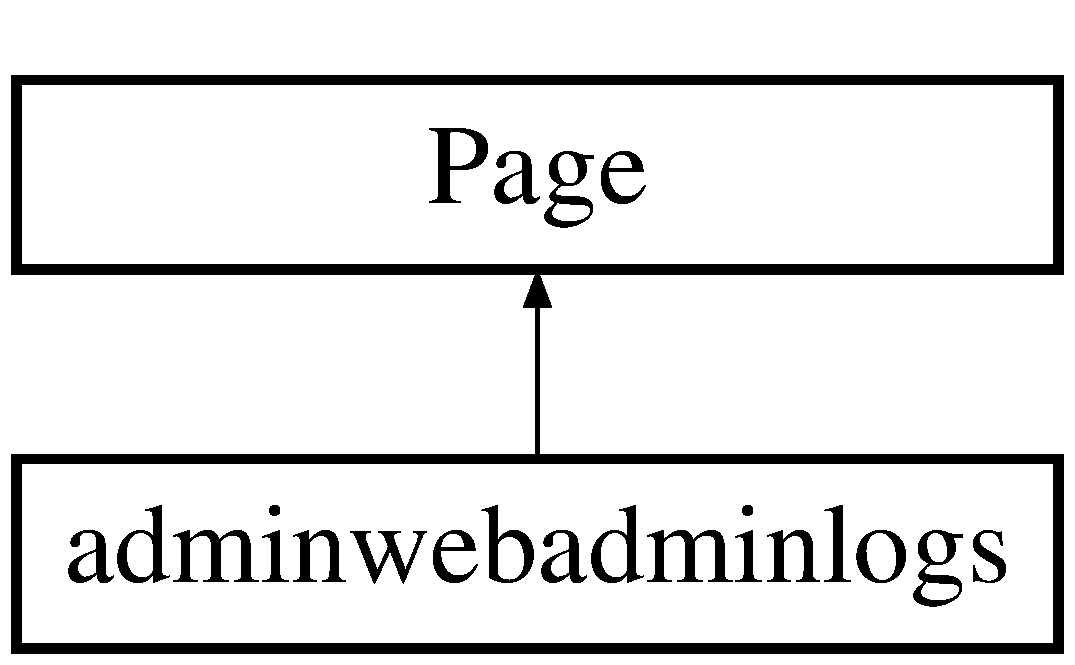
\includegraphics[height=2.000000cm]{classadminwebadminlogs}
\end{center}
\end{figure}
\subsection*{Protected Member Functions}
\begin{DoxyCompactItemize}
\item 
\hypertarget{classadminwebadminlogs_a112e47a92cea5703bcde8e53139034e8}{void {\bfseries Page\-\_\-\-Load} (object sender, Event\-Args e)}\label{classadminwebadminlogs_a112e47a92cea5703bcde8e53139034e8}

\item 
\hypertarget{classadminwebadminlogs_a686168f5aa0131e551a6d0cacf492e14}{void {\bfseries btnfilter\-\_\-\-Click} (object sender, Event\-Args e)}\label{classadminwebadminlogs_a686168f5aa0131e551a6d0cacf492e14}

\item 
\hypertarget{classadminwebadminlogs_a882bf3b005138152ef98e80d06c6641b}{void {\bfseries grdlogs\-\_\-\-Page\-Index\-Changing} (object sender, Grid\-View\-Page\-Event\-Args e)}\label{classadminwebadminlogs_a882bf3b005138152ef98e80d06c6641b}

\end{DoxyCompactItemize}


\subsection{Detailed Description}


Definition at line 9 of file adminwebadminlogs.\-aspx.\-cs.



The documentation for this class was generated from the following file\-:\begin{DoxyCompactItemize}
\item 
E\-:/\-Mint/\-Home care/\-Smart\-Home\-Care/adminwebadminlogs.\-aspx.\-cs\end{DoxyCompactItemize}

\hypertarget{class_base_serv}{\section{Base\-Serv Class Reference}
\label{class_base_serv}\index{Base\-Serv@{Base\-Serv}}
}


initialize the connection string to sql server  


Inheritance diagram for Base\-Serv\-:\begin{figure}[H]
\begin{center}
\leavevmode
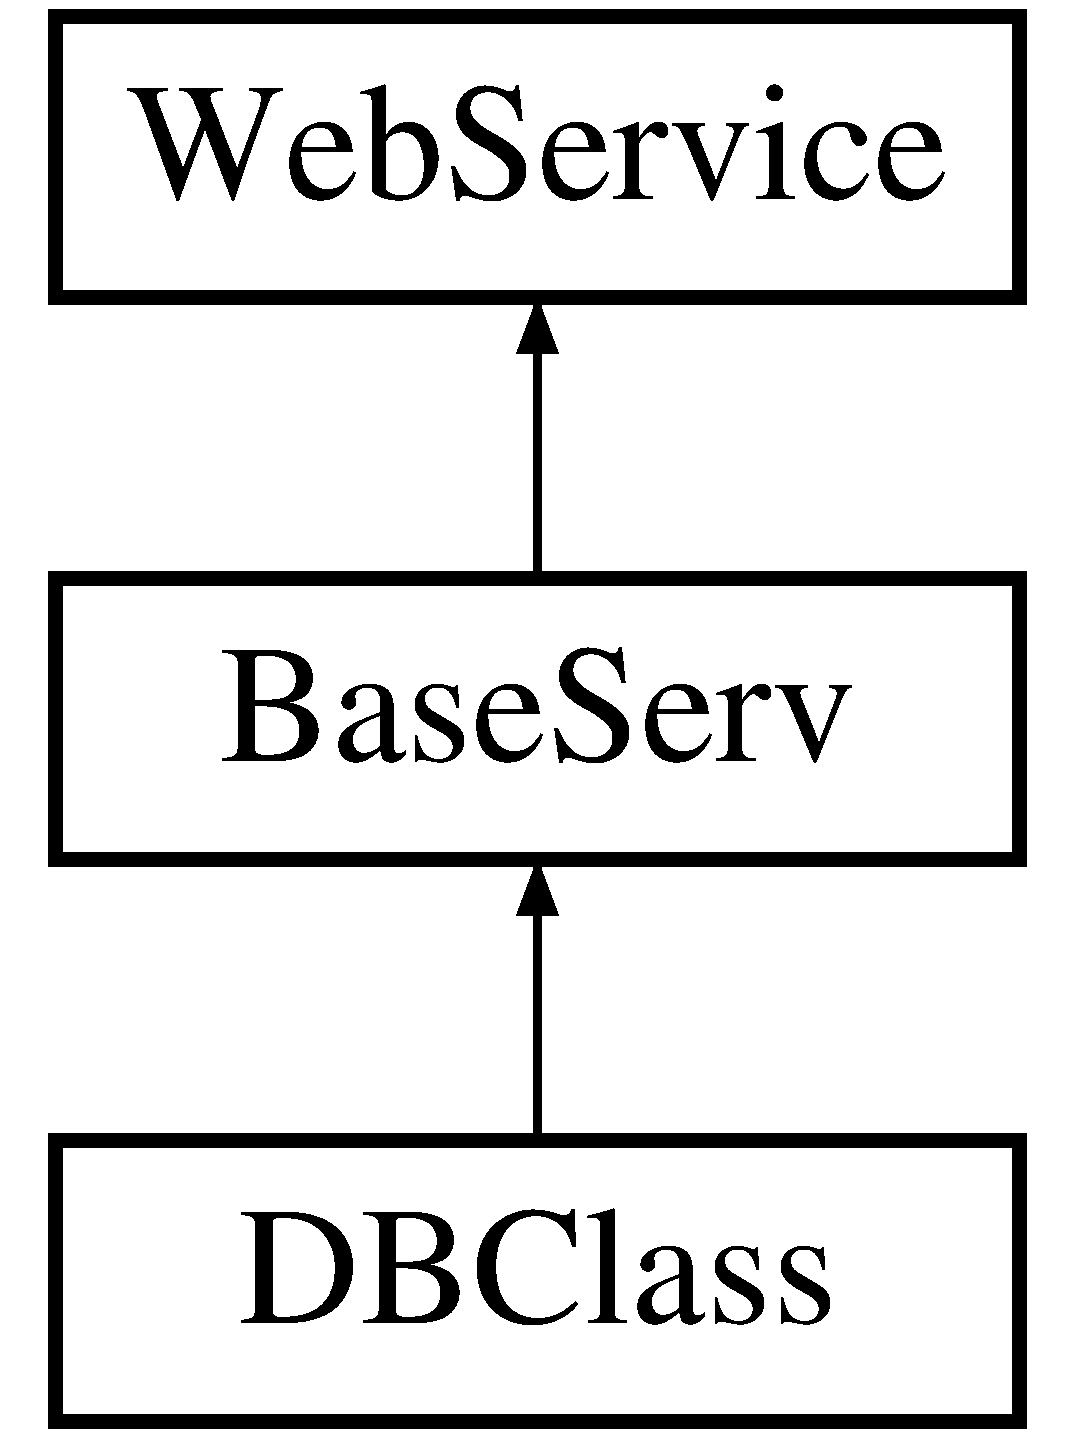
\includegraphics[height=3.000000cm]{class_base_serv}
\end{center}
\end{figure}
\subsection*{Static Protected Attributes}
\begin{DoxyCompactItemize}
\item 
\hypertarget{class_base_serv_a5ddc620c33beaae6c2e76912576d6c52}{static string {\bfseries db\-Conn\-String}}\label{class_base_serv_a5ddc620c33beaae6c2e76912576d6c52}

\end{DoxyCompactItemize}


\subsection{Detailed Description}
initialize the connection string to sql server 

Definition at line 16 of file Base\-Serv.\-cs.



The documentation for this class was generated from the following file\-:\begin{DoxyCompactItemize}
\item 
E\-:/\-Mint/\-Home care/\-Smart\-Home\-Care/\-App\-\_\-\-Code/Base\-Serv.\-cs\end{DoxyCompactItemize}

\hypertarget{class_base_view}{\section{Base\-View Class Reference}
\label{class_base_view}\index{Base\-View@{Base\-View}}
}


data processing , display on website  


\subsection*{Static Public Member Functions}
\begin{DoxyCompactItemize}
\item 
static void \hyperlink{class_base_view_add5facb001f67d1b233c739fd05f4522}{Selected\-Tree\-View} (Tree\-View tree, int parentnodeindex, int nodeindex=-\/1)
\item 
static void \hyperlink{class_base_view_a552808e7592fa857908c1cd62b962b62}{Bind\-Data\-To\-Dropdown\-List} (Drop\-Down\-List list, Data\-Table data, bool has\-None=true)
\item 
static void \hyperlink{class_base_view_a5c9efd93a389bbba53592f94e0c7e4bf}{Add\-Blank\-Dropdown\-Item} (Drop\-Down\-List list, string value=\char`\"{}\char`\"{})
\item 
static void \hyperlink{class_base_view_a11cb5505515d8022f035db42c6684ec4}{Add\-Blank\-Dropdown\-Item} (Drop\-Down\-List list, string text, string value)
\item 
static void \hyperlink{class_base_view_a9eefe3281f459553f95b598b8874b4ea}{Bind\-Data\-To\-List\-Box} (List\-Box list, Data\-Table data)
\item 
static void \hyperlink{class_base_view_a7c6c865233372bb21e52263d36dc06eb}{Select\-Dropdown\-Item} (Drop\-Down\-List list, object obj)
\item 
static void \hyperlink{class_base_view_af294e032b15c0d9f53e81a96db2c9847}{Select\-Dropdown\-Item} (Drop\-Down\-List list, string obj)
\item 
static bool \hyperlink{class_base_view_a9d7585ad518d5342c977dcaf50e4b98b}{Select\-Dropdown\-Item} (Drop\-Down\-List list, object obj, object enable)
\item 
static bool \hyperlink{class_base_view_a1ea899a45694c9a791f3bcbc0e53fe5d}{Check\-Image\-File\-Type} (string file\-Name)
\item 
static string \hyperlink{class_base_view_a980330f224af0bbc20a91d800cbf714a}{Html2\-Text} (string value)
\item 
static string \hyperlink{class_base_view_ac67acc0a12f0cf0a298a1f5a89eb4785}{Text2\-Html} (string value)
\item 
static object \hyperlink{class_base_view_a149c526459bc52ffc76d77110d8b55be}{Get\-Field\-Value} (Data\-Row\-View row, string Field\-Name)
\item 
\hypertarget{class_base_view_abefa3bdf34d884958b438d1b957a2b5d}{static string {\bfseries Get\-String\-Field\-Value} (Data\-Row\-View row, string Field\-Name)}\label{class_base_view_abefa3bdf34d884958b438d1b957a2b5d}

\item 
\hypertarget{class_base_view_aee131b709c6481077614865f7cbbce7a}{static int {\bfseries Get\-Int\-Field\-Value} (Data\-Row\-View row, string Field\-Name)}\label{class_base_view_aee131b709c6481077614865f7cbbce7a}

\item 
\hypertarget{class_base_view_aa056dee2dc0c2cd5ff34884361d8bd10}{static float {\bfseries Get\-Float\-Field\-Value} (Data\-Row\-View row, string Field\-Name)}\label{class_base_view_aa056dee2dc0c2cd5ff34884361d8bd10}

\item 
\hypertarget{class_base_view_ae379527e4bc9a1bca6cf2f77178417ad}{static bool {\bfseries Get\-Boolean\-Field\-Value} (Data\-Row\-View row, string Field\-Name)}\label{class_base_view_ae379527e4bc9a1bca6cf2f77178417ad}

\item 
\hypertarget{class_base_view_af613b200a3e6af0008709682f1e348ab}{static Date\-Time {\bfseries Get\-Date\-Time\-Field\-Value} (Data\-Row\-View row, string Field\-Name)}\label{class_base_view_af613b200a3e6af0008709682f1e348ab}

\item 
\hypertarget{class_base_view_aac24e88201088813b95a188e7dcef889}{static object {\bfseries Get\-Field\-Value} (Data\-Row row, string Field\-Name)}\label{class_base_view_aac24e88201088813b95a188e7dcef889}

\item 
\hypertarget{class_base_view_ac0018e7a447381abbee001b2e903c78c}{static string {\bfseries Get\-String\-Field\-Value} (Data\-Row row, string Field\-Name)}\label{class_base_view_ac0018e7a447381abbee001b2e903c78c}

\item 
\hypertarget{class_base_view_a9c6ebaafc61e2f042c55ee97189f1497}{static int {\bfseries Get\-Int\-Field\-Value} (Data\-Row row, string Field\-Name)}\label{class_base_view_a9c6ebaafc61e2f042c55ee97189f1497}

\item 
\hypertarget{class_base_view_a06679ddf26b8e36a6ce116952df39250}{static float {\bfseries Get\-Float\-Field\-Value} (Data\-Row row, string Field\-Name)}\label{class_base_view_a06679ddf26b8e36a6ce116952df39250}

\item 
\hypertarget{class_base_view_a0855871070c29d7033c50bcdd92e48b9}{static bool {\bfseries Get\-Boolean\-Field\-Value} (Data\-Row row, string Field\-Name)}\label{class_base_view_a0855871070c29d7033c50bcdd92e48b9}

\item 
\hypertarget{class_base_view_a5a1c6de2aebce9b7f327b78ea547b9cb}{static Date\-Time {\bfseries Get\-Date\-Time\-Field\-Value} (Data\-Row row, string Field\-Name)}\label{class_base_view_a5a1c6de2aebce9b7f327b78ea547b9cb}

\end{DoxyCompactItemize}


\subsection{Detailed Description}
data processing , display on website 

Definition at line 17 of file Base\-View.\-cs.



\subsection{Member Function Documentation}
\hypertarget{class_base_view_a5c9efd93a389bbba53592f94e0c7e4bf}{\index{Base\-View@{Base\-View}!Add\-Blank\-Dropdown\-Item@{Add\-Blank\-Dropdown\-Item}}
\index{Add\-Blank\-Dropdown\-Item@{Add\-Blank\-Dropdown\-Item}!BaseView@{Base\-View}}
\subsubsection[{Add\-Blank\-Dropdown\-Item}]{\setlength{\rightskip}{0pt plus 5cm}static void Base\-View.\-Add\-Blank\-Dropdown\-Item (
\begin{DoxyParamCaption}
\item[{Drop\-Down\-List}]{list, }
\item[{string}]{value = {\ttfamily \char`\"{}\char`\"{}}}
\end{DoxyParamCaption}
)\hspace{0.3cm}{\ttfamily [static]}}}\label{class_base_view_a5c9efd93a389bbba53592f94e0c7e4bf}
add 1 row to dropdownlist \begin{DoxySeeAlso}{See Also}
\hyperlink{class_base_view_a5c9efd93a389bbba53592f94e0c7e4bf}{Add\-Blank\-Dropdown\-Item()} 
\end{DoxySeeAlso}

\begin{DoxyParams}{Parameters}
{\em list} & control drop\-Down\-List of C\# \\
\hline
{\em value} & is dropdownlist \\
\hline
\end{DoxyParams}


Definition at line 101 of file Base\-View.\-cs.

\hypertarget{class_base_view_a11cb5505515d8022f035db42c6684ec4}{\index{Base\-View@{Base\-View}!Add\-Blank\-Dropdown\-Item@{Add\-Blank\-Dropdown\-Item}}
\index{Add\-Blank\-Dropdown\-Item@{Add\-Blank\-Dropdown\-Item}!BaseView@{Base\-View}}
\subsubsection[{Add\-Blank\-Dropdown\-Item}]{\setlength{\rightskip}{0pt plus 5cm}static void Base\-View.\-Add\-Blank\-Dropdown\-Item (
\begin{DoxyParamCaption}
\item[{Drop\-Down\-List}]{list, }
\item[{string}]{text, }
\item[{string}]{value}
\end{DoxyParamCaption}
)\hspace{0.3cm}{\ttfamily [static]}}}\label{class_base_view_a11cb5505515d8022f035db42c6684ec4}
add 1 row to dropdownlist \begin{DoxySeeAlso}{See Also}
\hyperlink{class_base_view_a5c9efd93a389bbba53592f94e0c7e4bf}{Add\-Blank\-Dropdown\-Item()} 
\end{DoxySeeAlso}

\begin{DoxyParams}{Parameters}
{\em list} & control drop\-Down\-List of C\# \\
\hline
{\em text} & is dropdownlist \\
\hline
{\em value} & is dropdownlist \\
\hline
\end{DoxyParams}


Definition at line 116 of file Base\-View.\-cs.

\hypertarget{class_base_view_a552808e7592fa857908c1cd62b962b62}{\index{Base\-View@{Base\-View}!Bind\-Data\-To\-Dropdown\-List@{Bind\-Data\-To\-Dropdown\-List}}
\index{Bind\-Data\-To\-Dropdown\-List@{Bind\-Data\-To\-Dropdown\-List}!BaseView@{Base\-View}}
\subsubsection[{Bind\-Data\-To\-Dropdown\-List}]{\setlength{\rightskip}{0pt plus 5cm}static void Base\-View.\-Bind\-Data\-To\-Dropdown\-List (
\begin{DoxyParamCaption}
\item[{Drop\-Down\-List}]{list, }
\item[{Data\-Table}]{data, }
\item[{bool}]{has\-None = {\ttfamily true}}
\end{DoxyParamCaption}
)\hspace{0.3cm}{\ttfamily [static]}}}\label{class_base_view_a552808e7592fa857908c1cd62b962b62}
bind data to dropdownlist \begin{DoxySeeAlso}{See Also}
\hyperlink{class_base_view_a552808e7592fa857908c1cd62b962b62}{Bind\-Data\-To\-Dropdown\-List()} 
\end{DoxySeeAlso}

\begin{DoxyParams}{Parameters}
{\em list} & control drop\-Down\-List of C\# \\
\hline
{\em data} & data\-Table is source of dropdownlist \\
\hline
{\em has\-None} & object(value\-: true or false) true\-: add dropdownlist 1 row none,false no add \\
\hline
\end{DoxyParams}


Definition at line 85 of file Base\-View.\-cs.

\hypertarget{class_base_view_a9eefe3281f459553f95b598b8874b4ea}{\index{Base\-View@{Base\-View}!Bind\-Data\-To\-List\-Box@{Bind\-Data\-To\-List\-Box}}
\index{Bind\-Data\-To\-List\-Box@{Bind\-Data\-To\-List\-Box}!BaseView@{Base\-View}}
\subsubsection[{Bind\-Data\-To\-List\-Box}]{\setlength{\rightskip}{0pt plus 5cm}static void Base\-View.\-Bind\-Data\-To\-List\-Box (
\begin{DoxyParamCaption}
\item[{List\-Box}]{list, }
\item[{Data\-Table}]{data}
\end{DoxyParamCaption}
)\hspace{0.3cm}{\ttfamily [static]}}}\label{class_base_view_a9eefe3281f459553f95b598b8874b4ea}
bind data to listbox \begin{DoxySeeAlso}{See Also}
\hyperlink{class_base_view_a9eefe3281f459553f95b598b8874b4ea}{Bind\-Data\-To\-List\-Box()} 
\end{DoxySeeAlso}

\begin{DoxyParams}{Parameters}
{\em list} & control List\-Box of C\# \\
\hline
{\em data} & data\-Table is source of List\-Box \\
\hline
\end{DoxyParams}


Definition at line 130 of file Base\-View.\-cs.

\hypertarget{class_base_view_a1ea899a45694c9a791f3bcbc0e53fe5d}{\index{Base\-View@{Base\-View}!Check\-Image\-File\-Type@{Check\-Image\-File\-Type}}
\index{Check\-Image\-File\-Type@{Check\-Image\-File\-Type}!BaseView@{Base\-View}}
\subsubsection[{Check\-Image\-File\-Type}]{\setlength{\rightskip}{0pt plus 5cm}static bool Base\-View.\-Check\-Image\-File\-Type (
\begin{DoxyParamCaption}
\item[{string}]{file\-Name}
\end{DoxyParamCaption}
)\hspace{0.3cm}{\ttfamily [static]}}}\label{class_base_view_a1ea899a45694c9a791f3bcbc0e53fe5d}
check file is image \begin{DoxySeeAlso}{See Also}
\hyperlink{class_base_view_a1ea899a45694c9a791f3bcbc0e53fe5d}{Check\-Image\-File\-Type()} 
\end{DoxySeeAlso}

\begin{DoxyParams}{Parameters}
{\em file\-Name} & is name image \\
\hline
\end{DoxyParams}


Definition at line 184 of file Base\-View.\-cs.

\hypertarget{class_base_view_a149c526459bc52ffc76d77110d8b55be}{\index{Base\-View@{Base\-View}!Get\-Field\-Value@{Get\-Field\-Value}}
\index{Get\-Field\-Value@{Get\-Field\-Value}!BaseView@{Base\-View}}
\subsubsection[{Get\-Field\-Value}]{\setlength{\rightskip}{0pt plus 5cm}static object Base\-View.\-Get\-Field\-Value (
\begin{DoxyParamCaption}
\item[{Data\-Row\-View}]{row, }
\item[{string}]{Field\-Name}
\end{DoxyParamCaption}
)\hspace{0.3cm}{\ttfamily [static]}}}\label{class_base_view_a149c526459bc52ffc76d77110d8b55be}
get value in datarow with column name 
\begin{DoxyParams}{Parameters}
{\em row} & is datarow or datarowview \\
\hline
{\em Field\-Name} & column name \\
\hline
\end{DoxyParams}


Definition at line 231 of file Base\-View.\-cs.

\hypertarget{class_base_view_a980330f224af0bbc20a91d800cbf714a}{\index{Base\-View@{Base\-View}!Html2\-Text@{Html2\-Text}}
\index{Html2\-Text@{Html2\-Text}!BaseView@{Base\-View}}
\subsubsection[{Html2\-Text}]{\setlength{\rightskip}{0pt plus 5cm}static string Base\-View.\-Html2\-Text (
\begin{DoxyParamCaption}
\item[{string}]{value}
\end{DoxyParamCaption}
)\hspace{0.3cm}{\ttfamily [static]}}}\label{class_base_view_a980330f224af0bbc20a91d800cbf714a}
convert text content from format html to text \begin{DoxySeeAlso}{See Also}
\hyperlink{class_base_view_a980330f224af0bbc20a91d800cbf714a}{Html2\-Text()} 
\end{DoxySeeAlso}

\begin{DoxyParams}{Parameters}
{\em value} & is text content \\
\hline
\end{DoxyParams}


Definition at line 211 of file Base\-View.\-cs.

\hypertarget{class_base_view_a7c6c865233372bb21e52263d36dc06eb}{\index{Base\-View@{Base\-View}!Select\-Dropdown\-Item@{Select\-Dropdown\-Item}}
\index{Select\-Dropdown\-Item@{Select\-Dropdown\-Item}!BaseView@{Base\-View}}
\subsubsection[{Select\-Dropdown\-Item}]{\setlength{\rightskip}{0pt plus 5cm}static void Base\-View.\-Select\-Dropdown\-Item (
\begin{DoxyParamCaption}
\item[{Drop\-Down\-List}]{list, }
\item[{object}]{obj}
\end{DoxyParamCaption}
)\hspace{0.3cm}{\ttfamily [static]}}}\label{class_base_view_a7c6c865233372bb21e52263d36dc06eb}
selected item of dropdownlist = object input \begin{DoxySeeAlso}{See Also}
\hyperlink{class_base_view_a7c6c865233372bb21e52263d36dc06eb}{Select\-Dropdown\-Item()} 
\end{DoxySeeAlso}

\begin{DoxyParams}{Parameters}
{\em list} & control Drop\-Down\-List of C\# \\
\hline
{\em obj} & is value input \\
\hline
\end{DoxyParams}


Definition at line 141 of file Base\-View.\-cs.

\hypertarget{class_base_view_af294e032b15c0d9f53e81a96db2c9847}{\index{Base\-View@{Base\-View}!Select\-Dropdown\-Item@{Select\-Dropdown\-Item}}
\index{Select\-Dropdown\-Item@{Select\-Dropdown\-Item}!BaseView@{Base\-View}}
\subsubsection[{Select\-Dropdown\-Item}]{\setlength{\rightskip}{0pt plus 5cm}static void Base\-View.\-Select\-Dropdown\-Item (
\begin{DoxyParamCaption}
\item[{Drop\-Down\-List}]{list, }
\item[{string}]{obj}
\end{DoxyParamCaption}
)\hspace{0.3cm}{\ttfamily [static]}}}\label{class_base_view_af294e032b15c0d9f53e81a96db2c9847}
selected item of dropdownlist = object input \begin{DoxySeeAlso}{See Also}
\hyperlink{class_base_view_a7c6c865233372bb21e52263d36dc06eb}{Select\-Dropdown\-Item()} 
\end{DoxySeeAlso}

\begin{DoxyParams}{Parameters}
{\em list} & control Drop\-Down\-List of C\# \\
\hline
{\em obj} & is value input \\
\hline
\end{DoxyParams}


Definition at line 157 of file Base\-View.\-cs.

\hypertarget{class_base_view_a9d7585ad518d5342c977dcaf50e4b98b}{\index{Base\-View@{Base\-View}!Select\-Dropdown\-Item@{Select\-Dropdown\-Item}}
\index{Select\-Dropdown\-Item@{Select\-Dropdown\-Item}!BaseView@{Base\-View}}
\subsubsection[{Select\-Dropdown\-Item}]{\setlength{\rightskip}{0pt plus 5cm}static bool Base\-View.\-Select\-Dropdown\-Item (
\begin{DoxyParamCaption}
\item[{Drop\-Down\-List}]{list, }
\item[{object}]{obj, }
\item[{object}]{enable}
\end{DoxyParamCaption}
)\hspace{0.3cm}{\ttfamily [static]}}}\label{class_base_view_a9d7585ad518d5342c977dcaf50e4b98b}
selected item of dropdownlist = object input \begin{DoxySeeAlso}{See Also}
\hyperlink{class_base_view_a7c6c865233372bb21e52263d36dc06eb}{Select\-Dropdown\-Item()} 
\end{DoxySeeAlso}

\begin{DoxyParams}{Parameters}
{\em list} & control Drop\-Down\-List of C\# \\
\hline
{\em obj} & is value input \\
\hline
\end{DoxyParams}


Definition at line 173 of file Base\-View.\-cs.

\hypertarget{class_base_view_add5facb001f67d1b233c739fd05f4522}{\index{Base\-View@{Base\-View}!Selected\-Tree\-View@{Selected\-Tree\-View}}
\index{Selected\-Tree\-View@{Selected\-Tree\-View}!BaseView@{Base\-View}}
\subsubsection[{Selected\-Tree\-View}]{\setlength{\rightskip}{0pt plus 5cm}static void Base\-View.\-Selected\-Tree\-View (
\begin{DoxyParamCaption}
\item[{Tree\-View}]{tree, }
\item[{int}]{parentnodeindex, }
\item[{int}]{nodeindex = {\ttfamily -\/1}}
\end{DoxyParamCaption}
)\hspace{0.3cm}{\ttfamily [static]}}}\label{class_base_view_add5facb001f67d1b233c739fd05f4522}
select index event handler directory tree ( left menu ) \begin{DoxySeeAlso}{See Also}
\hyperlink{class_base_view_add5facb001f67d1b233c739fd05f4522}{Selected\-Tree\-View()} 
\end{DoxySeeAlso}

\begin{DoxyParams}{Parameters}
{\em tree} & control treeview of C\# \\
\hline
{\em parentnodeindex} & node parent of node selected \\
\hline
{\em nodeindex} & node selected \\
\hline
\end{DoxyParams}


Definition at line 59 of file Base\-View.\-cs.

\hypertarget{class_base_view_ac67acc0a12f0cf0a298a1f5a89eb4785}{\index{Base\-View@{Base\-View}!Text2\-Html@{Text2\-Html}}
\index{Text2\-Html@{Text2\-Html}!BaseView@{Base\-View}}
\subsubsection[{Text2\-Html}]{\setlength{\rightskip}{0pt plus 5cm}static string Base\-View.\-Text2\-Html (
\begin{DoxyParamCaption}
\item[{string}]{value}
\end{DoxyParamCaption}
)\hspace{0.3cm}{\ttfamily [static]}}}\label{class_base_view_ac67acc0a12f0cf0a298a1f5a89eb4785}
convert text content from format text to html \begin{DoxySeeAlso}{See Also}
\hyperlink{class_base_view_ac67acc0a12f0cf0a298a1f5a89eb4785}{Text2\-Html()} 
\end{DoxySeeAlso}

\begin{DoxyParams}{Parameters}
{\em value} & is text content \\
\hline
\end{DoxyParams}


Definition at line 220 of file Base\-View.\-cs.



The documentation for this class was generated from the following file\-:\begin{DoxyCompactItemize}
\item 
E\-:/\-Mint/\-Home care/\-Smart\-Home\-Care/\-App\-\_\-\-Code/Base\-View.\-cs\end{DoxyCompactItemize}

\hypertarget{class_captcha_image}{\section{Captcha\-Image Class Reference}
\label{class_captcha_image}\index{Captcha\-Image@{Captcha\-Image}}
}


captcha processing  


\subsection*{Public Member Functions}
\begin{DoxyCompactItemize}
\item 
\hyperlink{class_captcha_image_addc88187074e1bc48f760181fe5346f6}{Captcha\-Image} (string s, int width, int height)
\item 
\hyperlink{class_captcha_image_adae3bb23f62acfffa6097cc94b35cbb8}{Captcha\-Image} (string s, int width, int height, string family\-Name)
\item 
void \hyperlink{class_captcha_image_ab19b4ea2bea72f095c1c009769cfe869}{Dispose} ()
\end{DoxyCompactItemize}
\subsection*{Protected Member Functions}
\begin{DoxyCompactItemize}
\item 
virtual void \hyperlink{class_captcha_image_a4fc7337f8a9fb18df976d23f65d6fa2a}{Dispose} (bool disposing)
\end{DoxyCompactItemize}
\subsection*{Properties}
\begin{DoxyCompactItemize}
\item 
string \hyperlink{class_captcha_image_a63d4fc8c2e707cbb26bb93a249032dc0}{Text}\hspace{0.3cm}{\ttfamily  \mbox{[}get\mbox{]}}
\item 
\hypertarget{class_captcha_image_af2c3c82cbfda08435a090f8e577afb58}{Bitmap {\bfseries Image}\hspace{0.3cm}{\ttfamily  \mbox{[}get\mbox{]}}}\label{class_captcha_image_af2c3c82cbfda08435a090f8e577afb58}

\item 
\hypertarget{class_captcha_image_a2e00afe7b142e38eb93504ef44b02b9a}{int {\bfseries Width}\hspace{0.3cm}{\ttfamily  \mbox{[}get\mbox{]}}}\label{class_captcha_image_a2e00afe7b142e38eb93504ef44b02b9a}

\item 
\hypertarget{class_captcha_image_a9ec050533e325e884f0e9c62dbe82f2d}{int {\bfseries Height}\hspace{0.3cm}{\ttfamily  \mbox{[}get\mbox{]}}}\label{class_captcha_image_a9ec050533e325e884f0e9c62dbe82f2d}

\end{DoxyCompactItemize}


\subsection{Detailed Description}
captcha processing 

Definition at line 10 of file Captcha\-Image.\-cs.



\subsection{Constructor \& Destructor Documentation}
\hypertarget{class_captcha_image_addc88187074e1bc48f760181fe5346f6}{\index{Captcha\-Image@{Captcha\-Image}!Captcha\-Image@{Captcha\-Image}}
\index{Captcha\-Image@{Captcha\-Image}!CaptchaImage@{Captcha\-Image}}
\subsubsection[{Captcha\-Image}]{\setlength{\rightskip}{0pt plus 5cm}Captcha\-Image.\-Captcha\-Image (
\begin{DoxyParamCaption}
\item[{string}]{s, }
\item[{int}]{width, }
\item[{int}]{height}
\end{DoxyParamCaption}
)}}\label{class_captcha_image_addc88187074e1bc48f760181fe5346f6}
Initializes a new instance of the \hyperlink{class_captcha_image}{Captcha\-Image} class using the specified text, width and height. 

Definition at line 50 of file Captcha\-Image.\-cs.

\hypertarget{class_captcha_image_adae3bb23f62acfffa6097cc94b35cbb8}{\index{Captcha\-Image@{Captcha\-Image}!Captcha\-Image@{Captcha\-Image}}
\index{Captcha\-Image@{Captcha\-Image}!CaptchaImage@{Captcha\-Image}}
\subsubsection[{Captcha\-Image}]{\setlength{\rightskip}{0pt plus 5cm}Captcha\-Image.\-Captcha\-Image (
\begin{DoxyParamCaption}
\item[{string}]{s, }
\item[{int}]{width, }
\item[{int}]{height, }
\item[{string}]{family\-Name}
\end{DoxyParamCaption}
)}}\label{class_captcha_image_adae3bb23f62acfffa6097cc94b35cbb8}
Initializes a new instance of the \hyperlink{class_captcha_image}{Captcha\-Image} class using the specified text, width, height and font family. 

Definition at line 61 of file Captcha\-Image.\-cs.



\subsection{Member Function Documentation}
\hypertarget{class_captcha_image_ab19b4ea2bea72f095c1c009769cfe869}{\index{Captcha\-Image@{Captcha\-Image}!Dispose@{Dispose}}
\index{Dispose@{Dispose}!CaptchaImage@{Captcha\-Image}}
\subsubsection[{Dispose}]{\setlength{\rightskip}{0pt plus 5cm}void Captcha\-Image.\-Dispose (
\begin{DoxyParamCaption}
{}
\end{DoxyParamCaption}
)}}\label{class_captcha_image_ab19b4ea2bea72f095c1c009769cfe869}
Releases all resources used by this object. 

Definition at line 80 of file Captcha\-Image.\-cs.

\hypertarget{class_captcha_image_a4fc7337f8a9fb18df976d23f65d6fa2a}{\index{Captcha\-Image@{Captcha\-Image}!Dispose@{Dispose}}
\index{Dispose@{Dispose}!CaptchaImage@{Captcha\-Image}}
\subsubsection[{Dispose}]{\setlength{\rightskip}{0pt plus 5cm}virtual void Captcha\-Image.\-Dispose (
\begin{DoxyParamCaption}
\item[{bool}]{disposing}
\end{DoxyParamCaption}
)\hspace{0.3cm}{\ttfamily [protected]}, {\ttfamily [virtual]}}}\label{class_captcha_image_a4fc7337f8a9fb18df976d23f65d6fa2a}
Custom Dispose method to clean up unmanaged resources. Dispose of the bitmap. 

Definition at line 89 of file Captcha\-Image.\-cs.



\subsection{Property Documentation}
\hypertarget{class_captcha_image_a63d4fc8c2e707cbb26bb93a249032dc0}{\index{Captcha\-Image@{Captcha\-Image}!Text@{Text}}
\index{Text@{Text}!CaptchaImage@{Captcha\-Image}}
\subsubsection[{Text}]{\setlength{\rightskip}{0pt plus 5cm}string Captcha\-Image.\-Text\hspace{0.3cm}{\ttfamily [get]}}}\label{class_captcha_image_a63d4fc8c2e707cbb26bb93a249032dc0}
Public properties (all read-\/only). 

Definition at line 16 of file Captcha\-Image.\-cs.



The documentation for this class was generated from the following file\-:\begin{DoxyCompactItemize}
\item 
E\-:/\-Mint/\-Home care/\-Smart\-Home\-Care/\-App\-\_\-\-Code/Captcha\-Image.\-cs\end{DoxyCompactItemize}

\hypertarget{class_data_service}{\section{Data\-Service Class Reference}
\label{class_data_service}\index{Data\-Service@{Data\-Service}}
}


Summary description for \hyperlink{class_data_service}{Data\-Service}  


Inheritance diagram for Data\-Service\-:\begin{figure}[H]
\begin{center}
\leavevmode
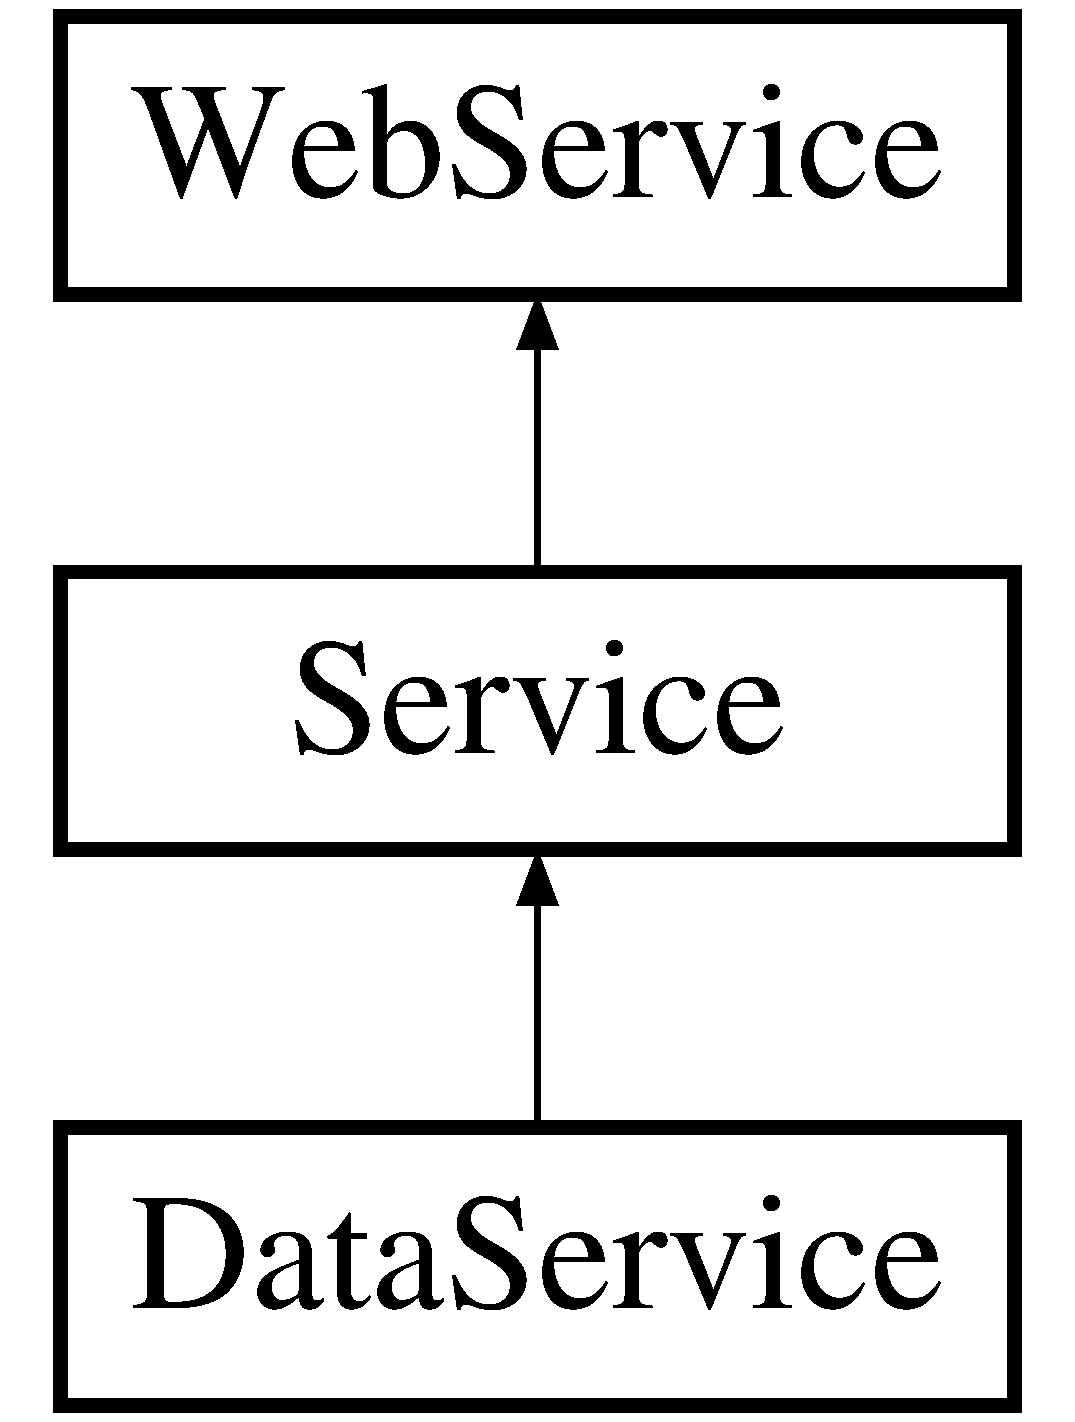
\includegraphics[height=3.000000cm]{class_data_service}
\end{center}
\end{figure}
\subsection*{Public Member Functions}
\begin{DoxyCompactItemize}
\item 
\hypertarget{class_data_service_a7670bef6be1600f66508d40b3efd2bed}{int {\bfseries Change\-Password} (string username, string passcurrent, string passnew, string passhint)}\label{class_data_service_a7670bef6be1600f66508d40b3efd2bed}

\item 
\hypertarget{class_data_service_a3a360a4987f916caf10b8da9a1d8f5b9}{int {\bfseries Delete\-\_\-\-Users\-Authorizes\-\_\-\-By\-Id} (int autoid)}\label{class_data_service_a3a360a4987f916caf10b8da9a1d8f5b9}

\item 
\hypertarget{class_data_service_af96d8f5aedcadd44e986bf2f3ff681f8}{int {\bfseries Insert\-Update\-\_\-\-Users} (string username, string userpass, string passhint, int usertypeid, bool isactive)}\label{class_data_service_af96d8f5aedcadd44e986bf2f3ff681f8}

\item 
\hypertarget{class_data_service_a7dff281418d38dd8e5acb13cd7593760}{int {\bfseries Insert\-Update\-\_\-\-Users\-Contact} (string username, string name, string email, string phone, string address, bool Is\-Main)}\label{class_data_service_a7dff281418d38dd8e5acb13cd7593760}

\item 
\hypertarget{class_data_service_a0a8c24a054193909af896bef4419de09}{int {\bfseries Insert\-Update\-\_\-\-Users\-Info} (string username, string firstname, string lastname, Date\-Time?dateofbirth, bool isgender, string emailaddress, string streetaddress, string citycode, string statecode, string zipcode, string county, string countrycode, string homephone, string mobilephone, string registrationcode)}\label{class_data_service_a0a8c24a054193909af896bef4419de09}

\item 
\hypertarget{class_data_service_a19746e61936a736cd426474f09c72355}{Xml\-Document {\bfseries Get\-Info\-\_\-\-Users\-All\-\_\-\-By\-User\-Name} (string username)}\label{class_data_service_a19746e61936a736cd426474f09c72355}

\item 
\hypertarget{class_data_service_ab0e59180d8f70f4be40d36bf2b6e03ac}{Xml\-Document {\bfseries Get\-List\-\_\-\-Member\-Type} ()}\label{class_data_service_ab0e59180d8f70f4be40d36bf2b6e03ac}

\item 
\hypertarget{class_data_service_a02a381a9505469814d5381baf638ec9d}{Xml\-Document {\bfseries Get\-Info\-\_\-\-Rule\-\_\-\-By\-User\-Name} (string username)}\label{class_data_service_a02a381a9505469814d5381baf638ec9d}

\item 
\hypertarget{class_data_service_aacd7dd284186b4392d62254ec90dd461}{Xml\-Document {\bfseries Get\-List\-\_\-\-Billing\-Account\-Types} ()}\label{class_data_service_aacd7dd284186b4392d62254ec90dd461}

\item 
\hypertarget{class_data_service_ae337f1b760ec16ab6dbba01c87e7d437}{Xml\-Document {\bfseries Get\-Info\-\_\-\-Users\-Contact\-\_\-\-By\-User\-Name} (string username)}\label{class_data_service_ae337f1b760ec16ab6dbba01c87e7d437}

\item 
\hypertarget{class_data_service_aad1b20cc373db62955a96e9e655a66b3}{Xml\-Document {\bfseries Get\-List\-\_\-\-Authorized\-User} (string username)}\label{class_data_service_aad1b20cc373db62955a96e9e655a66b3}

\item 
\hypertarget{class_data_service_ae05cb77ba2cea45e537c82e60403b895}{Xml\-Document {\bfseries Get\-List\-\_\-\-Countries} ()}\label{class_data_service_ae05cb77ba2cea45e537c82e60403b895}

\item 
\hypertarget{class_data_service_a94dc766f12634aa0c1d0e90d906bd333}{Xml\-Document {\bfseries Get\-List\-\_\-\-Country\-States} ()}\label{class_data_service_a94dc766f12634aa0c1d0e90d906bd333}

\item 
\hypertarget{class_data_service_a38798787831e7d83dfaca712b5d8da8b}{Xml\-Document {\bfseries Get\-List\-\_\-\-Credit\-Card\-Type} ()}\label{class_data_service_a38798787831e7d83dfaca712b5d8da8b}

\item 
\hypertarget{class_data_service_a461aa7b72d9db4100619f39d57b59202}{Xml\-Document {\bfseries Get\-List\-\_\-\-Country\-States\-\_\-\-By\-Country\-Code} (string countrycode)}\label{class_data_service_a461aa7b72d9db4100619f39d57b59202}

\item 
\hypertarget{class_data_service_acd21346bc33a7e622a8d604ca2446a5f}{Xml\-Document {\bfseries Insert\-\_\-\-Users\-Authorizes} (string username, string authorizeduser)}\label{class_data_service_acd21346bc33a7e622a8d604ca2446a5f}

\item 
\hypertarget{class_data_service_ab14ea2c933bad00c0d3b030efcbd6fdd}{Xml\-Document {\bfseries Login\-\_\-\-Website} (string username, string userpass, string loginfromcomputerip)}\label{class_data_service_ab14ea2c933bad00c0d3b030efcbd6fdd}

\item 
\hypertarget{class_data_service_a58f5413164d46b1427a6ba3d4025dabf}{Xml\-Document {\bfseries Register\-\_\-\-Account\-\_\-\-Users} (string username, string userpass, string passhint, string firstname, string lastname, Date\-Time?dateofbirth, bool isgender, string emailaddress, string streetaddress, string citycode, string statecode, string zipcode, string county, string countrycode, string homephone, string mobilephone, string registeredip, string registrationcode)}\label{class_data_service_a58f5413164d46b1427a6ba3d4025dabf}

\item 
\hypertarget{class_data_service_aaf06a5c5fa4d1b781c64ca1f38ffbd70}{object {\bfseries Register\-\_\-\-Validation\-\_\-\-User\-Name} (string username)}\label{class_data_service_aaf06a5c5fa4d1b781c64ca1f38ffbd70}

\item 
\hypertarget{class_data_service_a839b59fbd3ef0fa253e783ce76dcbd80}{object {\bfseries Is\-Exists\-\_\-\-Email} (string email)}\label{class_data_service_a839b59fbd3ef0fa253e783ce76dcbd80}

\item 
\hypertarget{class_data_service_ab1198c93d9b795505c292fb59eacece8}{Xml\-Document {\bfseries Submit\-\_\-\-Forgot\-\_\-\-Password} (string username, Date\-Time?dateofbirth)}\label{class_data_service_ab1198c93d9b795505c292fb59eacece8}

\item 
\hypertarget{class_data_service_a574c9fa71d43d11a3e285213d9c83d45}{Xml\-Document {\bfseries Submit\-\_\-\-Forgot\-\_\-\-User\-Name} (string firstname, string lastname, Date\-Time?dateofbirth, string zipcode)}\label{class_data_service_a574c9fa71d43d11a3e285213d9c83d45}

\item 
\hypertarget{class_data_service_ac43333e23d64c30fa58c76288db1f918}{Xml\-Document {\bfseries Get\-List\-\_\-\-Paramaters} (int Id, string Para\-Code, string Description)}\label{class_data_service_ac43333e23d64c30fa58c76288db1f918}

\item 
\hypertarget{class_data_service_a948d6a7651aab7079d03b2b20db850aa}{Xml\-Document {\bfseries Get\-List\-\_\-\-Admin\-Messages} (int Id, string Code, string Title)}\label{class_data_service_a948d6a7651aab7079d03b2b20db850aa}

\item 
\hypertarget{class_data_service_ac39fba49f63220713b78347998ff0890}{int {\bfseries Insert\-Update\-\_\-\-Admin\-Messages} (int Id, string Code, string Title, string Title\-V\-N, bool Approved, string Note)}\label{class_data_service_ac39fba49f63220713b78347998ff0890}

\item 
\hypertarget{class_data_service_a480553163cb3871f5d7b4650340e43bc}{Xml\-Document {\bfseries Get\-List\-\_\-\-Users\-\_\-\-Admin} (string User\-Name, string Last\-Name, string First\-Name, Date\-Time?From\-Date\-Of\-Birth, Date\-Time?To\-Date\-Of\-Birth)}\label{class_data_service_a480553163cb3871f5d7b4650340e43bc}

\item 
\hypertarget{class_data_service_ade287c6ebd7e84412ef3b6febe950369}{Xml\-Document {\bfseries Get\-List\-\_\-\-Users} (int userid, string username, bool?isactive, string email, Date\-Time?createdatefrom, Date\-Time?createdateto)}\label{class_data_service_ade287c6ebd7e84412ef3b6febe950369}

\item 
\hypertarget{class_data_service_a558deda59beb25d6023f672e48998960}{Xml\-Document {\bfseries Get\-List\-\_\-\-Register\-Codes} (string Rule, bool?Is\-Using, bool?Disable)}\label{class_data_service_a558deda59beb25d6023f672e48998960}

\item 
\hypertarget{class_data_service_ad16c9689171fb8c28740feee6829113d}{Xml\-Document {\bfseries Get\-List\-\_\-\-User\-\_\-\-Login} (string Username, Date\-Time?Login\-Date\-From, Date\-Time?Logind\-Date\-To)}\label{class_data_service_ad16c9689171fb8c28740feee6829113d}

\item 
\hypertarget{class_data_service_a29d0e6c75cf2e4d4066370613bc33e0d}{int {\bfseries Is\-Active\-\_\-\-User\-\_\-\-By\-Ids} (string Ids, bool is\-Active)}\label{class_data_service_a29d0e6c75cf2e4d4066370613bc33e0d}

\item 
\hypertarget{class_data_service_a45307371dd403c43dcc30466a78955a3}{int {\bfseries Insert\-Update\-\_\-\-Paramaters} (int Id, string Param\-Code, string Description, string Value, bool Active, string Note)}\label{class_data_service_a45307371dd403c43dcc30466a78955a3}

\item 
\hypertarget{class_data_service_a107244431463e7db7c8d8935dca02990}{int {\bfseries Delete\-Paramaters} (int Auto\-Id)}\label{class_data_service_a107244431463e7db7c8d8935dca02990}

\item 
\hypertarget{class_data_service_a91f53bd10b313175d3f651b21126b7ed}{int {\bfseries Set\-\_\-\-Register\-Code\-\_\-\-Using} (string Code)}\label{class_data_service_a91f53bd10b313175d3f651b21126b7ed}

\item 
\hypertarget{class_data_service_a27c7cbd088e31f6f3ede3946515e2a04}{Xml\-Document {\bfseries Insert\-\_\-\-Message\-Center} (string Mail\-From, string Subject, string Mail\-To, string Message\-Center)}\label{class_data_service_a27c7cbd088e31f6f3ede3946515e2a04}

\item 
\hypertarget{class_data_service_abd36617d72c34e8de2cc83d84ad81089}{Xml\-Document {\bfseries Delete\-\_\-\-Message\-Center\-\_\-\-By\-Ids} (string Message\-Ids)}\label{class_data_service_abd36617d72c34e8de2cc83d84ad81089}

\item 
\hypertarget{class_data_service_a715d6956951e3ec8d57688137b1110af}{Xml\-Document {\bfseries Delete\-\_\-\-Message\-Center\-\_\-\-Trash\-\_\-\-By\-Ids} (string Message\-Ids)}\label{class_data_service_a715d6956951e3ec8d57688137b1110af}

\item 
\hypertarget{class_data_service_a57a324d2ffcd220b3ecae8c6d79a6faf}{Xml\-Document {\bfseries Get\-Info\-\_\-\-Pay\-Bill\-\_\-\-Credit\-Card} (string username)}\label{class_data_service_a57a324d2ffcd220b3ecae8c6d79a6faf}

\item 
\hypertarget{class_data_service_a6c75eea9a18f8397d11f249d92176335}{Xml\-Document {\bfseries Get\-Info\-\_\-\-Billing\-Accounts} (string username)}\label{class_data_service_a6c75eea9a18f8397d11f249d92176335}

\item 
\hypertarget{class_data_service_a1d5027ccc0ec73f361207cfdddc952c8}{Xml\-Document {\bfseries Get\-Info\-\_\-\-Billing\-Accounts\-\_\-\-User} (string username)}\label{class_data_service_a1d5027ccc0ec73f361207cfdddc952c8}

\item 
\hypertarget{class_data_service_aba72984e816648a106c7fd0285952b51}{Xml\-Document {\bfseries Get\-List\-\_\-\-Billing\-Account\-Details} (string Account\-Number)}\label{class_data_service_aba72984e816648a106c7fd0285952b51}

\item 
\hypertarget{class_data_service_a2e68c5cc3fc4d870e34040f6f519397a}{Xml\-Document {\bfseries Get\-List\-\_\-\-Billing\-Payments} (string Account\-Number)}\label{class_data_service_a2e68c5cc3fc4d870e34040f6f519397a}

\item 
\hypertarget{class_data_service_aead21b3a7efd2a8287a5dd058d7aacd1}{Xml\-Document {\bfseries Get\-List\-\_\-\-Message\-Center\-\_\-\-Inbox} (string User\-Name)}\label{class_data_service_aead21b3a7efd2a8287a5dd058d7aacd1}

\item 
\hypertarget{class_data_service_ac271a75705166538f296173d3e999e6f}{Xml\-Document {\bfseries Get\-List\-\_\-\-Message\-Center\-\_\-\-Alarm} (string User\-Name)}\label{class_data_service_ac271a75705166538f296173d3e999e6f}

\item 
\hypertarget{class_data_service_a93139d269b2daddec457d61f89ce5008}{Xml\-Document {\bfseries Get\-List\-\_\-\-Message\-Center\-\_\-\-Sent} (string User\-Name)}\label{class_data_service_a93139d269b2daddec457d61f89ce5008}

\item 
\hypertarget{class_data_service_a8b482a47bc69c39b68a22d8298e6ace7}{Xml\-Document {\bfseries Get\-List\-\_\-\-Message\-Center\-\_\-\-Trash} (string User\-Name)}\label{class_data_service_a8b482a47bc69c39b68a22d8298e6ace7}

\item 
\hypertarget{class_data_service_a2fe4c1b40a299fd6fb5417f7cc1787df}{Xml\-Document {\bfseries Get\-Info\-\_\-\-Message\-Center\-\_\-\-By\-Id} (int Message\-Id)}\label{class_data_service_a2fe4c1b40a299fd6fb5417f7cc1787df}

\item 
\hypertarget{class_data_service_a89b2572b09a4b06c819f32c51c6a7983}{object {\bfseries Get\-Email\-\_\-\-By\-User\-Name} (string User\-Name)}\label{class_data_service_a89b2572b09a4b06c819f32c51c6a7983}

\item 
\hypertarget{class_data_service_ae2677cfdaa434fc5ebf1badd69d2c42b}{int {\bfseries Update\-Global\-Setting} (string User\-Name)}\label{class_data_service_ae2677cfdaa434fc5ebf1badd69d2c42b}

\item 
\hypertarget{class_data_service_a685a1941155b29f565f23b3accda2a8b}{Xml\-Document {\bfseries Get\-List\-\_\-\-User\-Temperature} (string User\-Name, Date\-Time?From\-Date, Date\-Time?To\-Date)}\label{class_data_service_a685a1941155b29f565f23b3accda2a8b}

\item 
\hypertarget{class_data_service_aff17bd0838bf8a0259193339cbb41115}{int {\bfseries Insert\-Update\-\_\-\-User\-Setting\-Color} (string User\-Name, int Skin\-Temp\-Color\-Id, int Amb\-Temp\-Color\-Id, int Background\-Color\-Id)}\label{class_data_service_aff17bd0838bf8a0259193339cbb41115}

\item 
\hypertarget{class_data_service_a26bde1ff50bb94037c7324af5ba4e795}{int {\bfseries Update\-\_\-\-Billing\-Account\-\_\-\-Management} (string Account\-Number, int Billing\-Type\-Id, Date\-Time?Eff\-Date, decimal Amount\-Charge, bool Is\-Pay\-Bill, string Notes)}\label{class_data_service_a26bde1ff50bb94037c7324af5ba4e795}

\item 
\hypertarget{class_data_service_a553d0998b3c0fbaea139f006de1a5c0f}{int {\bfseries Add\-Manual\-\_\-\-Billing\-Account\-\_\-\-Management} (string Account\-Number, Date\-Time?Date, decimal Amount\-Charge, string Notes)}\label{class_data_service_a553d0998b3c0fbaea139f006de1a5c0f}

\item 
\hypertarget{class_data_service_a2d26809cb72e2d690ed78a20b1301bba}{Xml\-Document {\bfseries Get\-Info\-\_\-\-User\-Track\-My\-Health} (string User\-Name)}\label{class_data_service_a2d26809cb72e2d690ed78a20b1301bba}

\item 
\hypertarget{class_data_service_a901c832f7c00ea5f037d3873c2eba919}{Xml\-Document {\bfseries Get\-Info\-\_\-\-User\-Setting\-Color} (string User\-Name)}\label{class_data_service_a901c832f7c00ea5f037d3873c2eba919}

\item 
\hypertarget{class_data_service_a17b86dc7d61f4881b8fdbfe1aa4b3dfc}{Xml\-Document {\bfseries Get\-Info\-\_\-\-User\-Track\-My\-Health\-\_\-\-Measurement} (string User\-Name)}\label{class_data_service_a17b86dc7d61f4881b8fdbfe1aa4b3dfc}

\item 
\hypertarget{class_data_service_a646fbf6e43038f0c6ea0b2e81332a2c8}{int {\bfseries Insert\-Update\-\_\-\-User\-Track\-My\-Health\-\_\-\-Measurement} (string User\-Name, bool Metric, bool U\-S)}\label{class_data_service_a646fbf6e43038f0c6ea0b2e81332a2c8}

\item 
\hypertarget{class_data_service_a8e57055390fa4c70cc327d862f157676}{int {\bfseries Insert\-Update\-\_\-\-User\-Track\-My\-Health\-\_\-\-Threshold} (string User\-Name, decimal?Samplerate, int?Sample\-Rate\-Id, decimal?Low\-Value, decimal?High\-Value, decimal?Very\-High\-Value)}\label{class_data_service_a8e57055390fa4c70cc327d862f157676}

\item 
\hypertarget{class_data_service_a0783c7cb8d0be5da111bd9353cd883e7}{Xml\-Document {\bfseries Get\-List\-\_\-\-User\-Track\-Others} (string User\-Name)}\label{class_data_service_a0783c7cb8d0be5da111bd9353cd883e7}

\item 
\hypertarget{class_data_service_a53cfbc56c02411ee0e4e4c8bacc11011}{Xml\-Document {\bfseries Get\-Info\-\_\-\-User\-All\-\_\-\-By\-User\-Name} (string User\-Name)}\label{class_data_service_a53cfbc56c02411ee0e4e4c8bacc11011}

\item 
\hypertarget{class_data_service_a79bde97cde64a0c63bfe46bc0ff792e5}{Xml\-Document {\bfseries Get\-Info\-\_\-\-Billing\-Info\-\_\-\-By\-Id} (string Payment\-Id)}\label{class_data_service_a79bde97cde64a0c63bfe46bc0ff792e5}

\item 
\hypertarget{class_data_service_acaf3126ea837032818951512ce95e8fd}{Xml\-Document {\bfseries Get\-List\-\_\-\-Email\-Templates} ()}\label{class_data_service_acaf3126ea837032818951512ce95e8fd}

\item 
\hypertarget{class_data_service_a1d7b5494f9c4716f965aeeb61763b3f0}{Xml\-Document {\bfseries Get\-Info\-\_\-\-Email\-Templates} (int Id)}\label{class_data_service_a1d7b5494f9c4716f965aeeb61763b3f0}

\item 
\hypertarget{class_data_service_a1f952e33f7595d80c902b0d52619ca9e}{int {\bfseries Insert\-Update\-\_\-\-Email\-Templates} (int id, string code, string subject, string body, string note)}\label{class_data_service_a1f952e33f7595d80c902b0d52619ca9e}

\item 
\hypertarget{class_data_service_a156854e6edb88cc7df5f3878246c3481}{bool {\bfseries Is\-Active\-\_\-\-User\-\_\-\-By\-Web\-Code} (string Web\-Code)}\label{class_data_service_a156854e6edb88cc7df5f3878246c3481}

\item 
\hypertarget{class_data_service_a0c07ab862e2dfd87bf1197b7df5e1a90}{string {\bfseries Insert\-\_\-\-Billing\-Info} (string Name\-Card, string Address, string Address\-Line2, string City, string State\-Code, string Z\-I\-P\-Code, string Country\-Code, string Phone, string Email, int Card\-Type\-Id, string Card\-Number, string Expiration\-Month, string Expiration\-Year, string Sercurity\-Code, string Account\-Number, decimal Amount\-Pay)}\label{class_data_service_a0c07ab862e2dfd87bf1197b7df5e1a90}

\item 
\hypertarget{class_data_service_a4838eb8b7d4979502fa6e218762f4cbc}{Xml\-Document {\bfseries Get\-Info\-\_\-\-User\-Overview} (string Username)}\label{class_data_service_a4838eb8b7d4979502fa6e218762f4cbc}

\item 
\hypertarget{class_data_service_a76b7287a917e2f3dd7b9d68a0a46eaa0}{int {\bfseries Update\-\_\-\-User\-Overview} (string User\-Name\-Old, string User\-Name\-New, string Email, string Warning, string Password)}\label{class_data_service_a76b7287a917e2f3dd7b9d68a0a46eaa0}

\item 
\hypertarget{class_data_service_abe3d14a65809c4c59c83b24561331df6}{int {\bfseries Get\-Value\-\_\-\-Paramter\-\_\-\-By\-Code} (string code)}\label{class_data_service_abe3d14a65809c4c59c83b24561331df6}

\item 
\hypertarget{class_data_service_a0b3d652fd7b4e8e416c8de91728ce50d}{string {\bfseries Invite\-\_\-\-Membertype} (string member\-Type)}\label{class_data_service_a0b3d652fd7b4e8e416c8de91728ce50d}

\item 
\hypertarget{class_data_service_ae8eed2a2ac838f1f87d0b2dc7fe559c4}{Xml\-Document {\bfseries Invalid\-\_\-\-Registration\-Code} (string registercode)}\label{class_data_service_ae8eed2a2ac838f1f87d0b2dc7fe559c4}

\end{DoxyCompactItemize}
\subsection*{Additional Inherited Members}


\subsection{Detailed Description}
Summary description for \hyperlink{class_data_service}{Data\-Service} 



Definition at line 16 of file Data\-Service.\-cs.



The documentation for this class was generated from the following file\-:\begin{DoxyCompactItemize}
\item 
E\-:/\-Mint/\-Home care/\-Smart\-Home\-Care/\-App\-\_\-\-Code/Data\-Service.\-cs\end{DoxyCompactItemize}

\hypertarget{class_d_b_class}{\section{D\-B\-Class Class Reference}
\label{class_d_b_class}\index{D\-B\-Class@{D\-B\-Class}}
}


select, insert, update, delete database sql server  


Inheritance diagram for D\-B\-Class\-:\begin{figure}[H]
\begin{center}
\leavevmode
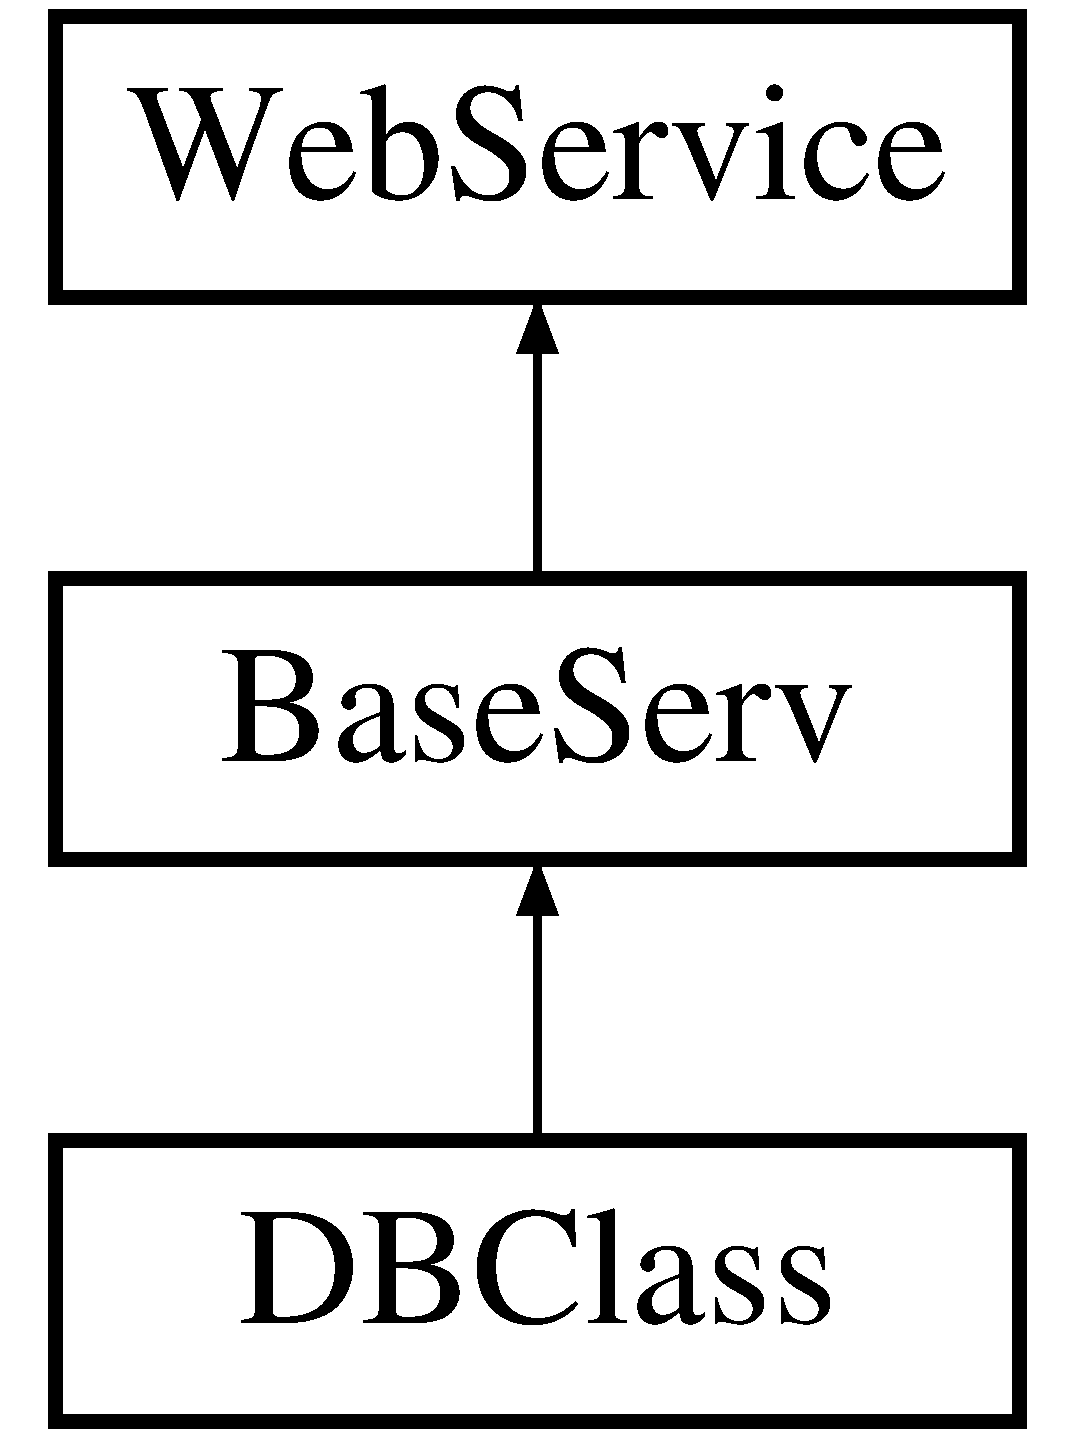
\includegraphics[height=3.000000cm]{class_d_b_class}
\end{center}
\end{figure}
\subsection*{Public Member Functions}
\begin{DoxyCompactItemize}
\item 
virtual object \hyperlink{class_d_b_class_a3995c60b4a603b90560f5180ae929348}{Execute\-Scalar} (string Procedure\-Name, params object\mbox{[}$\,$\mbox{]} Parameters)
\item 
virtual int \hyperlink{class_d_b_class_a9fe3e632d65861059ff2f8eb6c266a7b}{Execute\-Non\-Query} (string Procedure\-Name, params object\mbox{[}$\,$\mbox{]} Parameters)
\item 
virtual Data\-Row \hyperlink{class_d_b_class_a3d3793d07d5bdfcb8e904f1272f1e314}{Get\-Data\-Row} (string Procedure\-Name, params object\mbox{[}$\,$\mbox{]} Parameters)
\item 
virtual Data\-Row \hyperlink{class_d_b_class_af7d28bb6d82d5ed48310a9807148afea}{Get\-Data\-Row} (int Row\-Index, string Procedure\-Name, params object\mbox{[}$\,$\mbox{]} Parameters)
\item 
\hypertarget{class_d_b_class_a103c8b1a6b0d077064d2bef4b3b76c6b}{object {\bfseries Get\-Value\-From\-D\-B} (string sql)}\label{class_d_b_class_a103c8b1a6b0d077064d2bef4b3b76c6b}

\item 
int \hyperlink{class_d_b_class_ad7007450fd0cc27c1659da147b0d00e1}{Change\-Password} (string username, string passcurrent, string passnew, string passhint)
\item 
int \hyperlink{class_d_b_class_a24d9d653a4be300dd6136af86afadd1b}{Delete\-\_\-\-Users\-Authorizes\-\_\-\-By\-Id} (int autoid)
\item 
int \hyperlink{class_d_b_class_a26cddcc85c3f1be4d246912113d3a231}{Insert\-Update\-\_\-\-Users} (string username, string userpass, string passhint, int usertypeid, bool isactive)
\item 
int \hyperlink{class_d_b_class_a8900e70ea5308637f732de925c2e217b}{Insert\-Update\-\_\-\-Users\-Contact} (string username, string name, string email, string phone, string address, bool Is\-Main)
\item 
int \hyperlink{class_d_b_class_a9254bd810d437740310edb4fc6b19623}{Insert\-Update\-\_\-\-Users\-Info} (string username, string firstname, string lastname, Date\-Time?dateofbirth, bool isgender, string emailaddress, string streetaddress, string citycode, string statecode, string zipcode, string county, string countrycode, string homephone, string mobilephone, string registrationcode)
\item 
Data\-Row \hyperlink{class_d_b_class_a968aacf4f03ce8b3d11fdfeb72bd7301}{Get\-Info\-\_\-\-Users\-All\-\_\-\-By\-User\-Name} (string username)
\item 
Data\-Table \hyperlink{class_d_b_class_a68c8c13196578b5e88d1f8b831c95088}{Get\-List\-\_\-\-Member\-Type} ()
\item 
Data\-Row \hyperlink{class_d_b_class_a0db4839a470f33aa8e982bebddaaa001}{Get\-Info\-\_\-\-Rule\-\_\-\-By\-User\-Name} (string username)
\item 
Data\-Table \hyperlink{class_d_b_class_af38a7f3159f4c030237c6dd91db26a9d}{Get\-List\-\_\-\-Billing\-Account\-Types} ()
\item 
Data\-Row \hyperlink{class_d_b_class_a954ef42cfdb46f0757f30f088a60da27}{Get\-Info\-\_\-\-Users\-Contact\-\_\-\-By\-User\-Name} (string username)
\item 
Data\-Set \hyperlink{class_d_b_class_a6b82464db643c0331528f6a2fa6e7c69}{Get\-List\-\_\-\-Authorized\-User} (string username)
\item 
Data\-Set \hyperlink{class_d_b_class_a8306b2abf31bf8c5762e10945dcc6b69}{Get\-List\-\_\-\-Countries} ()
\item 
Data\-Set \hyperlink{class_d_b_class_ac33ddf061999a06d82c2e50f435972cc}{Get\-List\-\_\-\-Country\-States} ()
\item 
Data\-Set \hyperlink{class_d_b_class_a98f847d55e901665e418585ab706d4f4}{Get\-List\-\_\-\-Credit\-Card\-Type} ()
\item 
Data\-Set \hyperlink{class_d_b_class_a69f8d21cf730d614bdef36908ac343b3}{Get\-List\-\_\-\-Country\-States\-\_\-\-By\-Country\-Code} (string countrycode)
\item 
Data\-Row \hyperlink{class_d_b_class_ae4be85d37203b9423b92f4dd84a9a00d}{Insert\-\_\-\-Users\-Authorizes} (string username, string authorizeduser)
\item 
Data\-Row \hyperlink{class_d_b_class_aada5d4b0954419f23fcf368df799bd0c}{Login\-\_\-\-Website} (string username, string userpass, string loginfromcomputerip)
\item 
Data\-Row \hyperlink{class_d_b_class_ae7cb22c9fabc0e90288382a3d52c497c}{Register\-\_\-\-Account\-\_\-\-Users} (string username, string userpass, string passhint, string firstname, string lastname, Date\-Time?dateofbirth, bool isgender, string emailaddress, string streetaddress, string citycode, string statecode, string zipcode, string county, string countrycode, string homephone, string mobilephone, string registeredip, string registrationcode)
\item 
object \hyperlink{class_d_b_class_a08bd9c83614e63a7d978da2cde32d395}{Register\-\_\-\-Validation\-\_\-\-User\-Name} (string username)
\item 
object \hyperlink{class_d_b_class_a6e15594a3adc8194e932b15597421971}{Is\-Exists\-\_\-\-Email} (string email)
\item 
Data\-Row \hyperlink{class_d_b_class_a11e3e7a443614ac51a5a20155afb68b3}{Submit\-\_\-\-Forgot\-\_\-\-Password} (string username, Date\-Time?dateofbirth)
\item 
Data\-Row \hyperlink{class_d_b_class_a4946c6d4c6f92b0c79f64e8fe5bba494}{Submit\-\_\-\-Forgot\-\_\-\-User\-Name} (string firstname, string lastname, Date\-Time?dateofbirth, string zipcode)
\item 
Data\-Set \hyperlink{class_d_b_class_a46e602b287204bdccd5f684ed5cfddd1}{Get\-List\-\_\-\-Paramaters} (int Id, string Para\-Code, string Description)
\item 
Data\-Set \hyperlink{class_d_b_class_a37ba813f04c86f37ae0ff356c924daa3}{Get\-List\-\_\-\-Admin\-Messages} (int Id, string Code, string Title)
\item 
int \hyperlink{class_d_b_class_a839d19f3269b0cffbd7fad1600102b1a}{Insert\-Update\-\_\-\-Admin\-Messages} (int Id, string Code, string Title, string Title\-V\-N, bool Approved, string Note)
\item 
Data\-Set \hyperlink{class_d_b_class_a5988e32a4d26e9369010d22c45cd5047}{Get\-List\-\_\-\-Users\-\_\-\-Admin} (string User\-Name, string Last\-Name, string First\-Name, Date\-Time?From\-Date\-Of\-Birth, Date\-Time?To\-Date\-Of\-Birth)
\item 
Data\-Table \hyperlink{class_d_b_class_a878b22ac712481c277f9178b1b43fe07}{Get\-List\-\_\-\-Users} (int userid, string username, bool?isactive, string email, Date\-Time?createdatefrom, Date\-Time?createdateto)
\item 
Data\-Table \hyperlink{class_d_b_class_a5b9b462ffd2a0818dd1198a5d85db9b0}{Get\-List\-\_\-\-Register\-Codes} (string Rule, bool?Is\-Using, bool?Disable)
\item 
Data\-Table \hyperlink{class_d_b_class_a2d6d02138ea4f327cf81801671551727}{Get\-List\-\_\-\-User\-\_\-\-Login} (string Username, Date\-Time?Login\-Date\-From, Date\-Time?Logind\-Date\-To)
\item 
int \hyperlink{class_d_b_class_a4c5f9a9dc76a0b8585eeaf9fd3dcda9e}{Is\-Active\-\_\-\-User\-\_\-\-By\-Ids} (string Ids, bool is\-Active)
\item 
int \hyperlink{class_d_b_class_aa3330dd5a4961020f5da0bf0d0c66695}{Insert\-Update\-\_\-\-Paramaters} (int Id, string Param\-Code, string Description, string Value, bool Active, string Note)
\item 
int \hyperlink{class_d_b_class_a7ccd4c71dd6fae6380139ec0090d9b61}{Delete\-Paramaters} (int Auto\-Id)
\item 
int \hyperlink{class_d_b_class_aa77b93fa5b15252418e3fd8e24ffd8ac}{Set\-\_\-\-Register\-Code\-\_\-\-Using} (string Code)
\item 
Data\-Row \hyperlink{class_d_b_class_a14e9b463bcc808a13b42d55caca9b4ac}{Insert\-\_\-\-Message\-Center} (string Mail\-From, string Subject, string Mail\-To, string Message\-Center)
\item 
Data\-Row \hyperlink{class_d_b_class_a7db629c9df6c2c852dcf7eea76fb14a9}{Delete\-\_\-\-Message\-Center\-\_\-\-By\-Ids} (string Message\-Ids)
\item 
Data\-Row \hyperlink{class_d_b_class_a701df7b6a8ca9fc4ba08897cae80dfe8}{Delete\-\_\-\-Message\-Center\-\_\-\-Trash\-\_\-\-By\-Ids} (string Message\-Ids)
\item 
Data\-Row \hyperlink{class_d_b_class_a615a48cab9c51ef041a71bf4448cf4c4}{Get\-Info\-\_\-\-Pay\-Bill\-\_\-\-Credit\-Card} (string username)
\item 
Data\-Table \hyperlink{class_d_b_class_a55a667ccc7d91f17f481a874f287890f}{Get\-Info\-\_\-\-Billing\-Accounts} (string username)
\item 
Data\-Row \hyperlink{class_d_b_class_a2fc3997462f0ee4b552309ea63529a3a}{Get\-Info\-\_\-\-Billing\-Accounts\-\_\-\-User} (string username)
\item 
Data\-Table \hyperlink{class_d_b_class_a0401b205dab60659fa1b0d5e08a6380e}{Get\-List\-\_\-\-Billing\-Account\-Details} (string Account\-Number)
\item 
Data\-Table \hyperlink{class_d_b_class_a1325a85d94c5ca023962fe8b9be00d20}{Get\-List\-\_\-\-Billing\-Payments} (string Account\-Number)
\item 
Data\-Table \hyperlink{class_d_b_class_a8cc689495dd00f72cbb7ce4a1cf49e83}{Get\-List\-\_\-\-Message\-Center\-\_\-\-Inbox} (string User\-Name)
\item 
Data\-Table \hyperlink{class_d_b_class_a20a41495a3c7eeeb6e5d514374533e45}{Get\-List\-\_\-\-Message\-Center\-\_\-\-Alarm} (string User\-Name)
\item 
Data\-Table \hyperlink{class_d_b_class_ac6c5150b83d380d419fe3f2c21115e75}{Get\-List\-\_\-\-Message\-Center\-\_\-\-Sent} (string User\-Name)
\item 
Data\-Table \hyperlink{class_d_b_class_a945f0e551b6a114e9fc29a5a38928535}{Get\-List\-\_\-\-Message\-Center\-\_\-\-Trash} (string User\-Name)
\item 
Data\-Row \hyperlink{class_d_b_class_af0371885100aee5897fad3d19f1cabc4}{Get\-Info\-\_\-\-Message\-Center\-\_\-\-By\-Id} (int Message\-Id)
\item 
object \hyperlink{class_d_b_class_a708536f33fd79b8bbe0ddaff66ed643b}{Get\-Email\-\_\-\-By\-User\-Name} (string User\-Name)
\item 
int \hyperlink{class_d_b_class_a5be6a98dd7109e6bae4e4ff3ba9ef06a}{Update\-Global\-Setting} (string User\-Name)
\item 
Data\-Table \hyperlink{class_d_b_class_ac0a226a5b8778e0aa4bff3db3d0abb45}{Get\-List\-\_\-\-User\-Temperature} (string User\-Name, Date\-Time?From\-Date, Date\-Time?To\-Date)
\item 
int \hyperlink{class_d_b_class_a2efd80a5427a8bedc880acefd862553b}{Insert\-Update\-\_\-\-User\-Setting\-Color} (string User\-Name, int Skin\-Temp\-Color\-Id, int Amb\-Temp\-Color\-Id, int Background\-Color\-Id)
\item 
int \hyperlink{class_d_b_class_a3a0623cddd000fbd65ef3fbfc118e09d}{Update\-\_\-\-Billing\-Account\-\_\-\-Management} (string Account\-Number, int Billing\-Type\-Id, Date\-Time?Eff\-Date, decimal Amount\-Charge, bool Is\-Pay\-Bill, string Notes)
\item 
int \hyperlink{class_d_b_class_a3d44f9f299daf15fecc7bd0cc3c6ab2f}{Add\-Manual\-\_\-\-Billing\-Account\-\_\-\-Management} (string Account\-Number, Date\-Time?Date, decimal Amount\-Charge, string Notes)
\item 
Data\-Row \hyperlink{class_d_b_class_ae02372dc18e31565b4831363761727ce}{Get\-Info\-\_\-\-User\-Setting\-Color} (string User\-Name)
\item 
Data\-Row \hyperlink{class_d_b_class_ab25c43efd861fb5974df1edc2983a64d}{Get\-Info\-\_\-\-User\-Track\-My\-Health\-\_\-\-Measurement} (string User\-Name)
\item 
int \hyperlink{class_d_b_class_a4568088b863f4eced0d05dc68a255f7d}{Insert\-Update\-\_\-\-User\-Track\-My\-Health\-\_\-\-Measurement} (string User\-Name, bool Metric, bool U\-S)
\item 
Data\-Table \hyperlink{class_d_b_class_ac1ac9c6415e1f9754d2b40c3bb1ed5e4}{Get\-List\-\_\-\-User\-Track\-Others} (string User\-Name)
\item 
Data\-Table \hyperlink{class_d_b_class_a7beb5ee76c22290fbd4105d939f6f1db}{Get\-Info\-\_\-\-User\-All\-\_\-\-By\-User\-Name} (string User\-Name)
\item 
Data\-Table \hyperlink{class_d_b_class_a2c851e40cf0bde4ad893668dea5f4c8a}{Get\-Info\-\_\-\-Billing\-Info\-\_\-\-By\-Id} (string Payment\-Id)
\item 
Data\-Table \hyperlink{class_d_b_class_a92d17fbc58b19d0706febb49eac3af0c}{Get\-List\-\_\-\-Email\-Templates} ()
\item 
Data\-Table \hyperlink{class_d_b_class_af38b686d7f8458e55251e3b5b3c554d4}{Get\-Info\-\_\-\-Email\-Templates} (int Id)
\item 
int \hyperlink{class_d_b_class_adfc194b09f95c76cda91e3876e717399}{Insert\-Update\-\_\-\-Email\-Templates} (int id, string code, string subject, string body, string note)
\item 
bool \hyperlink{class_d_b_class_ad9d03a94de073831692a0ba77d9971eb}{Is\-Active\-\_\-\-User\-\_\-\-By\-Web\-Code} (string Web\-Code)
\item 
string \hyperlink{class_d_b_class_a516612b7d6008c48982987c8526a789e}{Insert\-\_\-\-Billing\-Info} (string Name\-Card, string Address, string Address\-Line2, string City, string State\-Code, string Z\-I\-P\-Code, string Country\-Code, string Phone, string Email, int Card\-Type\-Id, string Card\-Number, string Expiration\-Month, string Expiration\-Year, string Sercurity\-Code, string Account\-Number, decimal Amount\-Pay)
\item 
Data\-Row \hyperlink{class_d_b_class_a0fa08325a7d843fa631763b708fc32be}{Get\-Info\-\_\-\-User\-Overview} (string Username)
\item 
int \hyperlink{class_d_b_class_accdb33f185e3d071c73ed1c8c05c8db0}{Update\-\_\-\-User\-Overview} (string User\-Name\-Old, string User\-Name\-New, string Email, string Warning, string Password)
\item 
int \hyperlink{class_d_b_class_a547a707a154ff5ce5620445a986f9d80}{Get\-Value\-\_\-\-Paramter\-\_\-\-By\-Code} (string code)
\item 
string \hyperlink{class_d_b_class_a780a2360541eac03a5f601e807daa315}{Invite\-\_\-\-Membertype} (string member\-Type)
\item 
Data\-Row \hyperlink{class_d_b_class_a4d51d814947ee0d6b8e4fc40c69a9042}{Invalid\-\_\-\-Registration\-Code} (string registercode)
\item 
int \hyperlink{class_d_b_class_a0e5e201e2c1a800ef5f3bd6d27735a10}{Is\-Allow\-Check\-Status\-Registration\-Code\-In\-Send\-Email} ()
\item 
decimal \hyperlink{class_d_b_class_a95cc7b89b936bed76372b6cee5fac8bb}{Get\-\_\-\-Total\-Amount\-Due\-\_\-\-By\-Account\-Number} (string Account\-Number)
\item 
int \hyperlink{class_d_b_class_aead8cbe00c4eae2083023a1d4064da98}{Get\-Count\-\_\-\-Email\-Trash\-\_\-\-By\-User\-Name} (string User\-Name)
\item 
int \hyperlink{class_d_b_class_aa7e7e02bfe40b7f2cbbcb968245bcedf}{Get\-Count\-\_\-\-Email\-Sent\-\_\-\-By\-User\-Name} (string User\-Name)
\item 
int \hyperlink{class_d_b_class_a8eca9d29902373dde46eb6ff616b7f42}{Get\-Count\-\_\-\-Email\-Alarm\-\_\-\-By\-User\-Name} (string User\-Name)
\item 
int \hyperlink{class_d_b_class_a9314af57c8a3bc7bc95233f67892ed81}{Get\-Count\-\_\-\-Email\-New\-\_\-\-By\-User\-Name} (string User\-Name)
\item 
string \hyperlink{class_d_b_class_ae23b78ebc687ddc3e6ed4cc7db52eec8}{Get\-\_\-\-Registration\-Code\-\_\-\-By\-Member\-Type} (string membertype)
\item 
string \hyperlink{class_d_b_class_a8b1c1583c7deaf27f452d121c1ad06b3}{Get\-\_\-\-Registration\-Code\-\_\-\-Automatic} ()
\item 
bool \hyperlink{class_d_b_class_a18ad84f7d11d749b4a1d7eb633b5e6b4}{Get\-\_\-\-Is\-U\-S\-\_\-\-User\-Track\-My\-Health\-\_\-\-By\-User\-Name} (string username)
\item 
bool \hyperlink{class_d_b_class_ae14263d3318dc4b2ed3747c677bf98a2}{Is\-Invalid\-\_\-\-Email\-Address} (string username, string emailaddress)
\item 
string \hyperlink{class_d_b_class_aa1a72fda8621249f462071e883d14ead}{Cornfirm\-\_\-\-Delete} ()
\item 
string \hyperlink{class_d_b_class_a29ee46245e52b057a2a7e0d42cc72307}{Edit\-\_\-\-Success} ()
\item 
virtual Data\-Row \hyperlink{class_d_b_class_a101e80735fe6e717d5763d53eb772793}{Get\-Message\-By\-Code} (string message\-\_\-code)
\item 
Data\-Table \hyperlink{class_d_b_class_ab0a19e84d20ad1d00da1f6f2239153b3}{Get\-List\-\_\-\-Unit\-Time} ()
\item 
Data\-Table \hyperlink{class_d_b_class_aa17c75e306a63775128a29aa3682b98b}{Get\-List\-\_\-\-Unit\-Date} ()
\item 
int \hyperlink{class_d_b_class_ad222e776de0cc554f15903c20bd672f0}{Insert\-Update\-\_\-\-User\-Track\-My\-Health\-\_\-\-Threshold} (string User\-Name, decimal?Samplerate, int?Sample\-Rate\-Id, decimal?Low\-Value, decimal?High\-Value, decimal?Very\-High\-Value)
\item 
Data\-Row \hyperlink{class_d_b_class_ad9671a70651f9956eec03dbb5de3859e}{Get\-Info\-\_\-\-User\-Track\-My\-Health} (string User\-Name)
\item 
Data\-Table \hyperlink{class_d_b_class_af3711e9da9e4cc100a375496842590f5}{Get\-List\-\_\-\-Temperature\-\_\-\-Datetime} (string Username, Date\-Time?From\-Date, Date\-Time?To\-Date)
\item 
Data\-Table \hyperlink{class_d_b_class_a9bad7290fc0114ab60d343157dee22b1}{Get\-List\-\_\-\-Body\-B\-F\-Type} ()
\item 
Data\-Table \hyperlink{class_d_b_class_aa2a657479fe0ef609218bce4530f53ba}{Get\-List\-\_\-\-Body\-B\-M\-R\-Type} ()
\item 
Data\-Table \hyperlink{class_d_b_class_a0af97a662055ff2a3a41bcc3a28beaea}{Get\-List\-\_\-\-Datetime\-\_\-\-Body\-Measurement} (string username, Date\-Time?fromdate, Date\-Time?todate)
\item 
Data\-Table \hyperlink{class_d_b_class_ac3ab5f6a5dddad118d2a63c41b0b9f02}{Get\-List\-\_\-\-Body\-Measurement\-\_\-\-Table} (string username, Date\-Time?date)
\item 
Data\-Set \hyperlink{class_d_b_class_a416e75f38a46c9ab6607c740e175854f}{Get\-List\-\_\-\-Body\-Measurement\-\_\-\-Datatable} (string username, Date\-Time?fromdate, Date\-Time?todate)
\item 
Data\-Table \hyperlink{class_d_b_class_a0aabc831282182370eed262235495d33}{Get\-List\-\_\-\-Body\-Fat\-Eval} ()
\item 
Data\-Table \hyperlink{class_d_b_class_a85a6d769571f77eef926f08f7a88fe28}{Get\-List\-\_\-\-Body\-I\-W\-Type} ()
\item 
Data\-Table \hyperlink{class_d_b_class_a977ea5e7570c7bf8d20c9788161f60f6}{Get\-List\-\_\-\-Body\-Activity\-Factor\-Type} ()
\item 
Data\-Row \hyperlink{class_d_b_class_a1a96f514a3e855d11e45b296e3541b97}{Get\-Info\-\_\-\-Body\-Measurement} (string username)
\item 
int \hyperlink{class_d_b_class_a84a76caf413099a2f0f923f8a8c73f5a}{Insert\-Update\-\_\-\-Body\-Measurement\-\_\-\-U\-S} (int auto\-Id, string username, int?iwtypeid, int?bftypeid, int?bmrtypeid, int?fatevalid, int?activityfactortypeid, decimal?weight, decimal?heightfeet, decimal?heightinch, decimal?waist, decimal?hip, decimal?neck)
\item 
int \hyperlink{class_d_b_class_ac5833ce5d59ffc3703ca38bf5b337bc4}{Insert\-Update\-\_\-\-Body\-Measurement\-\_\-\-Metric} (int auto\-Id, string username, int?iwtypeid, int?bftypeid, int?bmrtypeid, int?fatevalid, int?activityfactortypeid, decimal?weight, decimal?height, decimal?waist, decimal?hip, decimal?neck)
\item 
Data\-Table \hyperlink{class_d_b_class_aa2228c10fe161653f3ee1a8938249747}{Get\-Info\-\_\-\-Body\-Measurement\-\_\-\-Graph} (string username)
\item 
Data\-Table \hyperlink{class_d_b_class_ae1b916fb79600663f47ddefb396223a1}{Get\-List\-\_\-\-Body\-Measurement\-\_\-\-Graph} (string User\-Name, Date\-Time?fromdate, Date\-Time?todate)
\item 
Data\-Table \hyperlink{class_d_b_class_aac1dfaf591ff86449a25f64d58c0c728}{Get\-List\-\_\-\-Heart\-Rate\-H\-R\-Est\-Type} ()
\item 
Data\-Table \hyperlink{class_d_b_class_a630396e518cffa1b479e83203c4010b4}{Get\-List\-\_\-\-Heart\-Rate\-\_\-\-Datetime} (string User\-Name, Date\-Time?From\-Date, Date\-Time?To\-Date)
\item 
Data\-Table \hyperlink{class_d_b_class_a9b7a23e13570beaa84677ee74d69476f}{Get\-List\-\_\-\-Unit\-B\-P\-M} ()
\item 
Data\-Row \hyperlink{class_d_b_class_a3e9f42bdd55ea3ced5e793bbbaa304e9}{Get\-Info\-\_\-\-Heart\-Rate} (string username)
\item 
int \hyperlink{class_d_b_class_aeb4a6084887a7e3c430af1513b4d7157}{Insert\-Update\-\_\-\-Heart\-Rate} (int auto\-Id, string username, decimal?samplerate, int?sr\-Unit\-Time\-Id, int?max\-H\-R\-Estimation\-Id, int?high\-Rest\-H\-R, int?low\-Rest\-H\-R, decimal?hrvanalysis\-Interal, int?hrv\-Unit\-Time\-Id)
\item 
Data\-Table \hyperlink{class_d_b_class_aa0781e64398da82d4b983a8b31a4ea4a}{Get\-List\-\_\-\-Heart\-Rate\-\_\-\-Table} (string username, Date\-Time?fromdate, Date\-Time?todate)
\item 
Data\-Set \hyperlink{class_d_b_class_a5910d9e2fcad738599583bb202daf3c9}{Get\-List\-\_\-\-Heart\-Rate\-\_\-\-H\-R\-V\-\_\-\-Table} (string username, Date\-Time?fromdate, Date\-Time?todate)
\item 
Data\-Set \hyperlink{class_d_b_class_a1aa2f0b88239718cb99cde4a77899437}{Get\-List\-\_\-\-Heart\-Rate\-\_\-\-H\-R\-V\-\_\-\-Graph} (string User\-Name, Date\-Time?fromdate, Date\-Time?todate)
\item 
Data\-Table \hyperlink{class_d_b_class_a78b75c0c3f63847fb9d747200630bdd7}{Get\-List\-\_\-\-Heart\-Rate\-\_\-\-Graph} (string User\-Name, Date\-Time?fromdate, Date\-Time?todate)
\item 
Data\-Row \hyperlink{class_d_b_class_a8e9823ed71afddef6b015fd2af946c3e}{Get\-Info\-\_\-\-Sp\-O2\-\_\-\-Tracking\-Mode\-Type} (int Id)
\item 
Data\-Row \hyperlink{class_d_b_class_aee73d7edc2d2f75e0c26d2d31597039e}{Get\-Info\-\_\-\-Sp\-O2} (string username)
\item 
Data\-Table \hyperlink{class_d_b_class_a052d4479aabdcaeb5f05ca76c0d8e166}{Get\-List\-\_\-\-Sp\-O2\-\_\-\-Tracking\-Mode\-Type} ()
\item 
object \hyperlink{class_d_b_class_a0e272870de72fd2dfe58a8077219d379}{Insert\-Update\-\_\-\-Sp\-O2} (int auto\-Id, string username, decimal?Sample\-Rate, int?Sample\-Rate\-Id, int?Tracking\-Type\-Id, decimal?Threshold, decimal?Measurement\-Value, int?Measurement\-Id)
\item 
Data\-Table \hyperlink{class_d_b_class_a2c9db13225c35720f41b7e051df5740f}{Get\-List\-\_\-\-Sp\-O2\-\_\-\-Table} (string User\-Name, Date\-Time?fromdate, Date\-Time?todate)
\item 
Data\-Table \hyperlink{class_d_b_class_a6f06d1414a7be6b9ddfed14f682e2205}{Get\-List\-\_\-\-Sp\-O2\-\_\-\-Graph} (string User\-Name, Date\-Time?fromdate, Date\-Time?todate)
\item 
Data\-Table \hyperlink{class_d_b_class_a816b02ee42e328f3283c8ec99423f720}{Get\-List\-\_\-\-Sp\-O2\-\_\-\-Datetime} (string User\-Name, Date\-Time?From\-Date, Date\-Time?To\-Date)
\item 
Data\-Table \hyperlink{class_d_b_class_a7962b2e3bd666862aeb6ef63a6fc5a30}{Get\-List\-\_\-\-Fitness\-\_\-\-H\-R\-Exercise\-Type} ()
\item 
Data\-Table \hyperlink{class_d_b_class_afe95c3d2857408582667370a34a4d88f}{Get\-List\-\_\-\-Fitness\-\_\-\-Datetime} (string User\-Name, Date\-Time?From\-Date, Date\-Time?To\-Date)
\item 
Data\-Table \hyperlink{class_d_b_class_a71298419ee709564e5c3074993c8e6d7}{Get\-List\-\_\-\-Fitness\-\_\-\-H\-R\-Target\-Type} ()
\item 
Data\-Table \hyperlink{class_d_b_class_a11af85d867a3a0c6c6a0e58d7cdeb5f8}{Get\-List\-\_\-\-Fitness\-\_\-\-H\-R\-Target\-Type\-\_\-\-Mutil} ()
\item 
Data\-Table \hyperlink{class_d_b_class_accf3ec92d4f585456ec3ff188e680fd3}{Get\-List\-\_\-\-Fitness\-\_\-\-H\-R\-Target\-Type\-\_\-\-Single} ()
\item 
Data\-Table \hyperlink{class_d_b_class_aee30d253f34099e058adde2106c19e4f}{Get\-List\-\_\-\-Fitness\-\_\-\-P\-M\-Target\-Type} ()
\item 
Data\-Table \hyperlink{class_d_b_class_a6814ee4c5e499dee4dca88ecb8f931e3}{Get\-List\-\_\-\-Fitness\-\_\-\-P\-M\-Remind\-Type} ()
\item 
Data\-Table \hyperlink{class_d_b_class_a82ded31f7b4ff63404618f1f668f4002}{Get\-List\-\_\-\-Fitness\-\_\-\-P\-M\-Calory\-Burn\-Type} ()
\item 
Data\-Row \hyperlink{class_d_b_class_ab7a630ce1c5e96d2a3430824a326299a}{Get\-Info\-\_\-\-Fitness} (string username)
\item 
int \hyperlink{class_d_b_class_a2d9bfec6c5e881fe884b8ad900368e49}{Insert\-Update\-\_\-\-Fitness} (int auto\-Id, string username, int?H\-R\-Exercise\-Id, int?H\-R\-Target\-Id, int?P\-M\-Target\-Id, int?P\-M\-Remind\-Id, int?P\-M\-Calory\-Burn\-Id)
\item 
Data\-Table \hyperlink{class_d_b_class_aca185474fc9923019ac4b4998d7212f5}{Get\-List\-\_\-\-Fitness\-\_\-\-Pedometer\-\_\-\-Table} (string User\-Name, Date\-Time?fromdate, Date\-Time?todate)
\item 
Data\-Table \hyperlink{class_d_b_class_a6b96de68a2a33aaa4438da7100c376c3}{Get\-List\-\_\-\-Fitness\-\_\-\-H\-R\-Exercise\-\_\-\-Table} (string User\-Name, Date\-Time?fromdate, Date\-Time?todate)
\item 
Data\-Table \hyperlink{class_d_b_class_a83af91ca1c0b7b98c951d8c70287218b}{Get\-List\-\_\-\-Fitness\-\_\-\-Pedometer\-\_\-\-Graph\-\_\-\-By\-Parameter\-Code} (string User\-Name, Date\-Time?From\-Date, Date\-Time?To\-Date, string Parameter\-Code)
\item 
Data\-Row \hyperlink{class_d_b_class_a7f44358ae70f852c5318bab2673d86ef}{Get\-Info\-\_\-\-Fitness\-\_\-\-H\-R\-Exercise\-\_\-\-Program\-\_\-\-By\-Fitness\-Id} (int fitness\-Id)
\item 
Data\-Table \hyperlink{class_d_b_class_a5be81c16e8893940b65e6cd7492d0517}{Get\-Info\-\_\-\-Fitness\-\_\-\-H\-R\-Exercise\-\_\-\-Program\-\_\-\-By\-Fitness\-H\-R\-Program\-Id} (int fitness\-H\-R\-Program\-Id)
\item 
Data\-Table \hyperlink{class_d_b_class_a7a5f310fffc8ab3a20bd33ac6e4312b6}{Get\-List\-\_\-\-Fitness\-\_\-\-Zone\-Type} ()
\item 
int \hyperlink{class_d_b_class_a2011973f0271030aa62150f5289d476f}{Insert\-Update\-\_\-\-Fitness\-\_\-\-H\-R\-Exercise\-\_\-\-Program} (int fitness\-Id, string user\-Name, int?number\-Of\-Stage, string program\-Name, string transition\-Audio)
\item 
int \hyperlink{class_d_b_class_a779173f60fc7e7d810f6c131f5d06896}{Insert\-Update\-\_\-\-Fitness\-\_\-\-H\-R\-Exercise\-\_\-\-Program\-\_\-\-Details} (int fitness\-H\-R\-Program\-Id, string stages, string zone\-Ids, string time\-Values, string time\-Ids)
\item 
Data\-Row \hyperlink{class_d_b_class_acf04cf47637571f88a6070d17e7ecd9d}{Get\-Info\-\_\-\-Stress} (string username)
\item 
int \hyperlink{class_d_b_class_adc8d1ca8c834e65325767f8187caf996}{Insert\-Update\-\_\-\-Stress} (int auto\-Id, string username, decimal?Measure\-Duration, int?M\-D\-Unit\-Time\-Id, decimal?H\-R\-Sample\-Rate, int?H\-R\-S\-R\-Unit\-Time\-Id, decimal?G\-S\-R\-Sample\-Rate, int?G\-S\-R\-S\-R\-Unit\-Time\-Id, decimal?Accel\-Sample\-Rate, int?A\-S\-R\-Unit\-Time\-Id)
\item 
Data\-Table \hyperlink{class_d_b_class_ad7d82013b592fb68b018a7a3a13f288a}{Get\-List\-\_\-\-Stress\-\_\-\-Rawdata\-\_\-\-Table} (string User\-Name, Date\-Time?fromdate, Date\-Time?todate)
\item 
Data\-Table \hyperlink{class_d_b_class_ae17050a8d003121b52345fca852c79ac}{Get\-List\-\_\-\-Stress\-\_\-\-Table} (string User\-Name, Date\-Time?From\-Date, Date\-Time?To\-Date)
\item 
Data\-Table \hyperlink{class_d_b_class_a197e91d6f8a237667be07dfa2bed6f43}{Get\-List\-\_\-\-Stress\-\_\-\-Rawdata\-\_\-\-Graph} (string User\-Name, Date\-Time?fromdate, Date\-Time?todate)
\item 
Data\-Table \hyperlink{class_d_b_class_a1795f539e4d1d2026a81813aa941729f}{Get\-List\-\_\-\-Stress\-\_\-\-Datetime} (string User\-Name, Date\-Time?From\-Date, Date\-Time?To\-Date)
\item 
Data\-Row \hyperlink{class_d_b_class_a5facb048821017872ad28def8ed62069}{Get\-Info\-\_\-\-Fertility} (string username)
\item 
object \hyperlink{class_d_b_class_af1fff159bbd1c80d087c8ca4b429482e}{Insert\-Update\-\_\-\-Fertility} (int Auto\-Id, string username, bool Is\-Input\-Auto)
\item 
Data\-Table \hyperlink{class_d_b_class_ae1fcea41ffa99821225730266d6d8d51}{Get\-List\-\_\-\-Fertility\-\_\-\-Table} (string User\-Name, Date\-Time?From\-Date, Date\-Time?To\-Date)
\item 
Data\-Table \hyperlink{class_d_b_class_aebf1652426c1b3f3bfb9a8866b60def1}{Get\-List\-\_\-\-Fertility\-\_\-\-Temperature} (string User\-Name, Date\-Time From\-Date, Date\-Time To\-Date)
\item 
Data\-Table \hyperlink{class_d_b_class_a6f81c3255588664f2c43d3c0440c9c43}{Get\-List\-\_\-\-Fertility\-\_\-\-Graph} (string User\-Name, Date\-Time From\-Date, Date\-Time To\-Date)
\item 
Data\-Row \hyperlink{class_d_b_class_acbbbf8d9d956c84edccb36e85bc240e3}{Get\-Info\-\_\-\-Position} (string username)
\item 
int \hyperlink{class_d_b_class_a42021171f10d36c06c7c77b9628743f9}{Insert\-Update\-\_\-\-Position} (int auto\-Id, string username, decimal?Sample\-Rate, int?Sample\-Rate\-Id, bool Is\-Supine, bool Is\-Prone, bool Is\-Left, bool Is\-Right, bool Is\-Up, bool Is\-Down)
\item 
Data\-Table \hyperlink{class_d_b_class_ab13e332c43c442cebd09a18406a6860e}{Get\-List\-\_\-\-Position\-\_\-\-Table} (string User\-Name, Date\-Time?fromdate, Date\-Time?todate)
\item 
Data\-Table \hyperlink{class_d_b_class_ae651f2f8ee54772f41b82ce0c03dcab9}{Get\-List\-\_\-\-Position\-\_\-\-Graph} (string User\-Name, Date\-Time?From\-Date, Date\-Time?To\-Date)
\item 
Data\-Table \hyperlink{class_d_b_class_aa7a8aba6f4ab18f61d5a358d6ac7c613}{Get\-List\-\_\-\-Position\-\_\-\-X\-Y\-Z\-\_\-\-Rawdata\-\_\-\-Table} (string User\-Name, Date\-Time?fromdate, Date\-Time?todate)
\item 
Data\-Table \hyperlink{class_d_b_class_a59adf109e871a062c0cda615e710f895}{Get\-List\-\_\-\-Position\-\_\-\-Datetime} (string User\-Name, Date\-Time?From\-Date, Date\-Time?To\-Date)
\item 
Data\-Table \hyperlink{class_d_b_class_a82e1217fb79406dc76a8afc1315b2c46}{Get\-List\-\_\-\-Sleep\-\_\-\-Datetime} (string User\-Name, Date\-Time?From\-Date, Date\-Time?To\-Date)
\item 
Data\-Row \hyperlink{class_d_b_class_af30a4aa2b39b452b77380ae85ff365f4}{Get\-Info\-\_\-\-Sleep} (string username)
\item 
int \hyperlink{class_d_b_class_a00b39101f9f39e20fc7e10307ab3c06f}{Insert\-Update\-\_\-\-Sleep} (int auto\-Id, string username, decimal?H\-R\-Sample\-Rate, int?H\-R\-Sample\-Rate\-Id, decimal?G\-S\-R\-Sample\-Rate, int?G\-S\-R\-Sample\-Rate\-Id, decimal?Acc\-Sample\-Rate, int?Acc\-Sample\-Rate\-Id, decimal?Skin\-Temp\-Sample\-Rate, int?Skin\-Temp\-Sample\-Rate\-Id, bool Is\-Alarm\-Setting, decimal?Sleep\-Duration, int?Sleep\-Duration\-Id)
\item 
Data\-Table \hyperlink{class_d_b_class_a0e2606c8a08dfa94868f871b6ab8f848}{Get\-List\-\_\-\-Sleep\-\_\-\-Manual\-\_\-\-By\-Sleep\-Id} (int Sleep\-Id)
\item 
int \hyperlink{class_d_b_class_a68f701aa5999c1bdc92e2d880b7d41af}{Insert\-Update\-\_\-\-Sleep\-\_\-\-Manual} (int sleep\-Id, string names, string unit\-Date\-Ids, string unit\-Time\-Values, string unit\-Time\-Ids)
\item 
Data\-Table \hyperlink{class_d_b_class_ae619d8b6adac22347a9b9a302d45a5f5}{Get\-List\-\_\-\-Sleep\-\_\-\-Rawdata} (string User\-Name, Date\-Time?fromdate, Date\-Time?todate)
\end{DoxyCompactItemize}
\subsection*{Static Public Member Functions}
\begin{DoxyCompactItemize}
\item 
static Data\-Table \hyperlink{class_d_b_class_ab3e7318b0c12986f5b4bbf566a1aec32}{Get\-Data\-Table} (int Table\-Index, string Procedure\-Name, params object\mbox{[}$\,$\mbox{]} Parameters)
\item 
static Data\-Table \hyperlink{class_d_b_class_a7ba7be30e81075831d240a4c905ac650}{Get\-Data\-Table} (string Procedure\-Name, params object\mbox{[}$\,$\mbox{]} Parameters)
\item 
static Data\-Set \hyperlink{class_d_b_class_a4061cee8189ba6ee8c6ebf19be8567dc}{Get\-Data\-Set} (string Procedure\-Name, params object\mbox{[}$\,$\mbox{]} Parameters)
\item 
static string \hyperlink{class_d_b_class_a2d0699b41086dd4e043fa2c653543f94}{Get\-Message\-By\-Code2} (string message\-\_\-code)
\end{DoxyCompactItemize}
\subsection*{Additional Inherited Members}


\subsection{Detailed Description}
select, insert, update, delete database sql server 

Definition at line 14 of file D\-B\-Class.\-cs.



\subsection{Member Function Documentation}
\hypertarget{class_d_b_class_a3d44f9f299daf15fecc7bd0cc3c6ab2f}{\index{D\-B\-Class@{D\-B\-Class}!Add\-Manual\-\_\-\-Billing\-Account\-\_\-\-Management@{Add\-Manual\-\_\-\-Billing\-Account\-\_\-\-Management}}
\index{Add\-Manual\-\_\-\-Billing\-Account\-\_\-\-Management@{Add\-Manual\-\_\-\-Billing\-Account\-\_\-\-Management}!DBClass@{D\-B\-Class}}
\subsubsection[{Add\-Manual\-\_\-\-Billing\-Account\-\_\-\-Management}]{\setlength{\rightskip}{0pt plus 5cm}int D\-B\-Class.\-Add\-Manual\-\_\-\-Billing\-Account\-\_\-\-Management (
\begin{DoxyParamCaption}
\item[{string}]{Account\-Number, }
\item[{Date\-Time?}]{Date, }
\item[{decimal}]{Amount\-Charge, }
\item[{string}]{Notes}
\end{DoxyParamCaption}
)}}\label{class_d_b_class_a3d44f9f299daf15fecc7bd0cc3c6ab2f}
add manual billing account \begin{DoxySeeAlso}{See Also}
\hyperlink{class_d_b_class_a3d44f9f299daf15fecc7bd0cc3c6ab2f}{Add\-Manual\-\_\-\-Billing\-Account\-\_\-\-Management()} 
\end{DoxySeeAlso}
\begin{DoxyReturn}{Returns}
int value 1 success, 0 failure 
\end{DoxyReturn}


Definition at line 641 of file D\-B\-Class.\-cs.

\hypertarget{class_d_b_class_ad7007450fd0cc27c1659da147b0d00e1}{\index{D\-B\-Class@{D\-B\-Class}!Change\-Password@{Change\-Password}}
\index{Change\-Password@{Change\-Password}!DBClass@{D\-B\-Class}}
\subsubsection[{Change\-Password}]{\setlength{\rightskip}{0pt plus 5cm}int D\-B\-Class.\-Change\-Password (
\begin{DoxyParamCaption}
\item[{string}]{username, }
\item[{string}]{passcurrent, }
\item[{string}]{passnew, }
\item[{string}]{passhint}
\end{DoxyParamCaption}
)}}\label{class_d_b_class_ad7007450fd0cc27c1659da147b0d00e1}
change password user \begin{DoxySeeAlso}{See Also}
\hyperlink{class_d_b_class_ad7007450fd0cc27c1659da147b0d00e1}{Change\-Password()} 
\end{DoxySeeAlso}

\begin{DoxyParams}{Parameters}
{\em username} & need change password \\
\hline
{\em pascurrent} & password current \\
\hline
{\em passnew} & password new need change \\
\hline
\end{DoxyParams}
\begin{DoxyReturn}{Returns}
value 1 success, 0 failure 
\end{DoxyReturn}


Definition at line 130 of file D\-B\-Class.\-cs.

\hypertarget{class_d_b_class_aa1a72fda8621249f462071e883d14ead}{\index{D\-B\-Class@{D\-B\-Class}!Cornfirm\-\_\-\-Delete@{Cornfirm\-\_\-\-Delete}}
\index{Cornfirm\-\_\-\-Delete@{Cornfirm\-\_\-\-Delete}!DBClass@{D\-B\-Class}}
\subsubsection[{Cornfirm\-\_\-\-Delete}]{\setlength{\rightskip}{0pt plus 5cm}string D\-B\-Class.\-Cornfirm\-\_\-\-Delete (
\begin{DoxyParamCaption}
{}
\end{DoxyParamCaption}
)}}\label{class_d_b_class_aa1a72fda8621249f462071e883d14ead}
message box confirm delete \begin{DoxySeeAlso}{See Also}
\hyperlink{class_d_b_class_aa1a72fda8621249f462071e883d14ead}{Cornfirm\-\_\-\-Delete()} 
\end{DoxySeeAlso}
\begin{DoxyReturn}{Returns}
string value 
\end{DoxyReturn}


Definition at line 930 of file D\-B\-Class.\-cs.

\hypertarget{class_d_b_class_a7db629c9df6c2c852dcf7eea76fb14a9}{\index{D\-B\-Class@{D\-B\-Class}!Delete\-\_\-\-Message\-Center\-\_\-\-By\-Ids@{Delete\-\_\-\-Message\-Center\-\_\-\-By\-Ids}}
\index{Delete\-\_\-\-Message\-Center\-\_\-\-By\-Ids@{Delete\-\_\-\-Message\-Center\-\_\-\-By\-Ids}!DBClass@{D\-B\-Class}}
\subsubsection[{Delete\-\_\-\-Message\-Center\-\_\-\-By\-Ids}]{\setlength{\rightskip}{0pt plus 5cm}Data\-Row D\-B\-Class.\-Delete\-\_\-\-Message\-Center\-\_\-\-By\-Ids (
\begin{DoxyParamCaption}
\item[{string}]{Message\-Ids}
\end{DoxyParamCaption}
)}}\label{class_d_b_class_a7db629c9df6c2c852dcf7eea76fb14a9}
delete message by array id \begin{DoxySeeAlso}{See Also}
\hyperlink{class_d_b_class_a7db629c9df6c2c852dcf7eea76fb14a9}{Delete\-\_\-\-Message\-Center\-\_\-\-By\-Ids()} 
\end{DoxySeeAlso}
\begin{DoxyReturn}{Returns}
datarow 
\end{DoxyReturn}


Definition at line 476 of file D\-B\-Class.\-cs.

\hypertarget{class_d_b_class_a701df7b6a8ca9fc4ba08897cae80dfe8}{\index{D\-B\-Class@{D\-B\-Class}!Delete\-\_\-\-Message\-Center\-\_\-\-Trash\-\_\-\-By\-Ids@{Delete\-\_\-\-Message\-Center\-\_\-\-Trash\-\_\-\-By\-Ids}}
\index{Delete\-\_\-\-Message\-Center\-\_\-\-Trash\-\_\-\-By\-Ids@{Delete\-\_\-\-Message\-Center\-\_\-\-Trash\-\_\-\-By\-Ids}!DBClass@{D\-B\-Class}}
\subsubsection[{Delete\-\_\-\-Message\-Center\-\_\-\-Trash\-\_\-\-By\-Ids}]{\setlength{\rightskip}{0pt plus 5cm}Data\-Row D\-B\-Class.\-Delete\-\_\-\-Message\-Center\-\_\-\-Trash\-\_\-\-By\-Ids (
\begin{DoxyParamCaption}
\item[{string}]{Message\-Ids}
\end{DoxyParamCaption}
)}}\label{class_d_b_class_a701df7b6a8ca9fc4ba08897cae80dfe8}
delete message trash by array trash id \begin{DoxySeeAlso}{See Also}
\hyperlink{class_d_b_class_a701df7b6a8ca9fc4ba08897cae80dfe8}{Delete\-\_\-\-Message\-Center\-\_\-\-Trash\-\_\-\-By\-Ids()} 
\end{DoxySeeAlso}
\begin{DoxyReturn}{Returns}
datarow 
\end{DoxyReturn}


Definition at line 485 of file D\-B\-Class.\-cs.

\hypertarget{class_d_b_class_a24d9d653a4be300dd6136af86afadd1b}{\index{D\-B\-Class@{D\-B\-Class}!Delete\-\_\-\-Users\-Authorizes\-\_\-\-By\-Id@{Delete\-\_\-\-Users\-Authorizes\-\_\-\-By\-Id}}
\index{Delete\-\_\-\-Users\-Authorizes\-\_\-\-By\-Id@{Delete\-\_\-\-Users\-Authorizes\-\_\-\-By\-Id}!DBClass@{D\-B\-Class}}
\subsubsection[{Delete\-\_\-\-Users\-Authorizes\-\_\-\-By\-Id}]{\setlength{\rightskip}{0pt plus 5cm}int D\-B\-Class.\-Delete\-\_\-\-Users\-Authorizes\-\_\-\-By\-Id (
\begin{DoxyParamCaption}
\item[{int}]{autoid}
\end{DoxyParamCaption}
)}}\label{class_d_b_class_a24d9d653a4be300dd6136af86afadd1b}
delete user authorize by id \begin{DoxySeeAlso}{See Also}
\hyperlink{class_d_b_class_a24d9d653a4be300dd6136af86afadd1b}{Delete\-\_\-\-Users\-Authorizes\-\_\-\-By\-Id()} 
\end{DoxySeeAlso}

\begin{DoxyParams}{Parameters}
{\em autoid} & id user authorize need delete \\
\hline
\end{DoxyParams}
\begin{DoxyReturn}{Returns}
value 1 success, 0 failure 
\end{DoxyReturn}


Definition at line 142 of file D\-B\-Class.\-cs.

\hypertarget{class_d_b_class_a7ccd4c71dd6fae6380139ec0090d9b61}{\index{D\-B\-Class@{D\-B\-Class}!Delete\-Paramaters@{Delete\-Paramaters}}
\index{Delete\-Paramaters@{Delete\-Paramaters}!DBClass@{D\-B\-Class}}
\subsubsection[{Delete\-Paramaters}]{\setlength{\rightskip}{0pt plus 5cm}int D\-B\-Class.\-Delete\-Paramaters (
\begin{DoxyParamCaption}
\item[{int}]{Auto\-Id}
\end{DoxyParamCaption}
)}}\label{class_d_b_class_a7ccd4c71dd6fae6380139ec0090d9b61}
delete parameter by id \begin{DoxySeeAlso}{See Also}
\hyperlink{class_d_b_class_a7ccd4c71dd6fae6380139ec0090d9b61}{Delete\-Paramaters()} 
\end{DoxySeeAlso}
\begin{DoxyReturn}{Returns}
int value 1 success, 0 failure 
\end{DoxyReturn}


Definition at line 448 of file D\-B\-Class.\-cs.

\hypertarget{class_d_b_class_a29ee46245e52b057a2a7e0d42cc72307}{\index{D\-B\-Class@{D\-B\-Class}!Edit\-\_\-\-Success@{Edit\-\_\-\-Success}}
\index{Edit\-\_\-\-Success@{Edit\-\_\-\-Success}!DBClass@{D\-B\-Class}}
\subsubsection[{Edit\-\_\-\-Success}]{\setlength{\rightskip}{0pt plus 5cm}string D\-B\-Class.\-Edit\-\_\-\-Success (
\begin{DoxyParamCaption}
{}
\end{DoxyParamCaption}
)}}\label{class_d_b_class_a29ee46245e52b057a2a7e0d42cc72307}
message box confirm edit \begin{DoxySeeAlso}{See Also}
\hyperlink{class_d_b_class_a29ee46245e52b057a2a7e0d42cc72307}{Edit\-\_\-\-Success()} 
\end{DoxySeeAlso}
\begin{DoxyReturn}{Returns}
string value 
\end{DoxyReturn}


Definition at line 939 of file D\-B\-Class.\-cs.

\hypertarget{class_d_b_class_a9fe3e632d65861059ff2f8eb6c266a7b}{\index{D\-B\-Class@{D\-B\-Class}!Execute\-Non\-Query@{Execute\-Non\-Query}}
\index{Execute\-Non\-Query@{Execute\-Non\-Query}!DBClass@{D\-B\-Class}}
\subsubsection[{Execute\-Non\-Query}]{\setlength{\rightskip}{0pt plus 5cm}virtual int D\-B\-Class.\-Execute\-Non\-Query (
\begin{DoxyParamCaption}
\item[{string}]{Procedure\-Name, }
\item[{params object\mbox{[}$\,$\mbox{]}}]{Parameters}
\end{DoxyParamCaption}
)\hspace{0.3cm}{\ttfamily [virtual]}}}\label{class_d_b_class_a9fe3e632d65861059ff2f8eb6c266a7b}
execute procedure insert, update, delete \begin{DoxySeeAlso}{See Also}
\hyperlink{class_d_b_class_a9fe3e632d65861059ff2f8eb6c266a7b}{Execute\-Non\-Query()} 
\end{DoxySeeAlso}
\begin{DoxyReturn}{Returns}
int 
\end{DoxyReturn}


Definition at line 37 of file D\-B\-Class.\-cs.

\hypertarget{class_d_b_class_a3995c60b4a603b90560f5180ae929348}{\index{D\-B\-Class@{D\-B\-Class}!Execute\-Scalar@{Execute\-Scalar}}
\index{Execute\-Scalar@{Execute\-Scalar}!DBClass@{D\-B\-Class}}
\subsubsection[{Execute\-Scalar}]{\setlength{\rightskip}{0pt plus 5cm}virtual object D\-B\-Class.\-Execute\-Scalar (
\begin{DoxyParamCaption}
\item[{string}]{Procedure\-Name, }
\item[{params object\mbox{[}$\,$\mbox{]}}]{Parameters}
\end{DoxyParamCaption}
)\hspace{0.3cm}{\ttfamily [virtual]}}}\label{class_d_b_class_a3995c60b4a603b90560f5180ae929348}
execute procedure insert, update, delete \begin{DoxySeeAlso}{See Also}
\hyperlink{class_d_b_class_a3995c60b4a603b90560f5180ae929348}{Execute\-Scalar()} 
\end{DoxySeeAlso}
\begin{DoxyReturn}{Returns}
object 
\end{DoxyReturn}


Definition at line 28 of file D\-B\-Class.\-cs.

\hypertarget{class_d_b_class_a18ad84f7d11d749b4a1d7eb633b5e6b4}{\index{D\-B\-Class@{D\-B\-Class}!Get\-\_\-\-Is\-U\-S\-\_\-\-User\-Track\-My\-Health\-\_\-\-By\-User\-Name@{Get\-\_\-\-Is\-U\-S\-\_\-\-User\-Track\-My\-Health\-\_\-\-By\-User\-Name}}
\index{Get\-\_\-\-Is\-U\-S\-\_\-\-User\-Track\-My\-Health\-\_\-\-By\-User\-Name@{Get\-\_\-\-Is\-U\-S\-\_\-\-User\-Track\-My\-Health\-\_\-\-By\-User\-Name}!DBClass@{D\-B\-Class}}
\subsubsection[{Get\-\_\-\-Is\-U\-S\-\_\-\-User\-Track\-My\-Health\-\_\-\-By\-User\-Name}]{\setlength{\rightskip}{0pt plus 5cm}bool D\-B\-Class.\-Get\-\_\-\-Is\-U\-S\-\_\-\-User\-Track\-My\-Health\-\_\-\-By\-User\-Name (
\begin{DoxyParamCaption}
\item[{string}]{username}
\end{DoxyParamCaption}
)}}\label{class_d_b_class_a18ad84f7d11d749b4a1d7eb633b5e6b4}
check user is U\-S \begin{DoxySeeAlso}{See Also}
\hyperlink{class_d_b_class_a18ad84f7d11d749b4a1d7eb633b5e6b4}{Get\-\_\-\-Is\-U\-S\-\_\-\-User\-Track\-My\-Health\-\_\-\-By\-User\-Name()} 
\end{DoxySeeAlso}
\begin{DoxyReturn}{Returns}
bool value 
\end{DoxyReturn}


Definition at line 903 of file D\-B\-Class.\-cs.

\hypertarget{class_d_b_class_a8b1c1583c7deaf27f452d121c1ad06b3}{\index{D\-B\-Class@{D\-B\-Class}!Get\-\_\-\-Registration\-Code\-\_\-\-Automatic@{Get\-\_\-\-Registration\-Code\-\_\-\-Automatic}}
\index{Get\-\_\-\-Registration\-Code\-\_\-\-Automatic@{Get\-\_\-\-Registration\-Code\-\_\-\-Automatic}!DBClass@{D\-B\-Class}}
\subsubsection[{Get\-\_\-\-Registration\-Code\-\_\-\-Automatic}]{\setlength{\rightskip}{0pt plus 5cm}string D\-B\-Class.\-Get\-\_\-\-Registration\-Code\-\_\-\-Automatic (
\begin{DoxyParamCaption}
{}
\end{DoxyParamCaption}
)}}\label{class_d_b_class_a8b1c1583c7deaf27f452d121c1ad06b3}
get string register code automatic \begin{DoxySeeAlso}{See Also}
\hyperlink{class_d_b_class_a8b1c1583c7deaf27f452d121c1ad06b3}{Get\-\_\-\-Registration\-Code\-\_\-\-Automatic()} 
\end{DoxySeeAlso}
\begin{DoxyReturn}{Returns}
string value 
\end{DoxyReturn}


Definition at line 891 of file D\-B\-Class.\-cs.

\hypertarget{class_d_b_class_ae23b78ebc687ddc3e6ed4cc7db52eec8}{\index{D\-B\-Class@{D\-B\-Class}!Get\-\_\-\-Registration\-Code\-\_\-\-By\-Member\-Type@{Get\-\_\-\-Registration\-Code\-\_\-\-By\-Member\-Type}}
\index{Get\-\_\-\-Registration\-Code\-\_\-\-By\-Member\-Type@{Get\-\_\-\-Registration\-Code\-\_\-\-By\-Member\-Type}!DBClass@{D\-B\-Class}}
\subsubsection[{Get\-\_\-\-Registration\-Code\-\_\-\-By\-Member\-Type}]{\setlength{\rightskip}{0pt plus 5cm}string D\-B\-Class.\-Get\-\_\-\-Registration\-Code\-\_\-\-By\-Member\-Type (
\begin{DoxyParamCaption}
\item[{string}]{membertype}
\end{DoxyParamCaption}
)}}\label{class_d_b_class_ae23b78ebc687ddc3e6ed4cc7db52eec8}
get string code by membertype \begin{DoxySeeAlso}{See Also}
\hyperlink{class_d_b_class_ae23b78ebc687ddc3e6ed4cc7db52eec8}{Get\-\_\-\-Registration\-Code\-\_\-\-By\-Member\-Type()} 
\end{DoxySeeAlso}
\begin{DoxyReturn}{Returns}
string value 
\end{DoxyReturn}


Definition at line 879 of file D\-B\-Class.\-cs.

\hypertarget{class_d_b_class_a95cc7b89b936bed76372b6cee5fac8bb}{\index{D\-B\-Class@{D\-B\-Class}!Get\-\_\-\-Total\-Amount\-Due\-\_\-\-By\-Account\-Number@{Get\-\_\-\-Total\-Amount\-Due\-\_\-\-By\-Account\-Number}}
\index{Get\-\_\-\-Total\-Amount\-Due\-\_\-\-By\-Account\-Number@{Get\-\_\-\-Total\-Amount\-Due\-\_\-\-By\-Account\-Number}!DBClass@{D\-B\-Class}}
\subsubsection[{Get\-\_\-\-Total\-Amount\-Due\-\_\-\-By\-Account\-Number}]{\setlength{\rightskip}{0pt plus 5cm}decimal D\-B\-Class.\-Get\-\_\-\-Total\-Amount\-Due\-\_\-\-By\-Account\-Number (
\begin{DoxyParamCaption}
\item[{string}]{Account\-Number}
\end{DoxyParamCaption}
)}}\label{class_d_b_class_a95cc7b89b936bed76372b6cee5fac8bb}
get total amount due by account number \begin{DoxySeeAlso}{See Also}
\hyperlink{class_d_b_class_a95cc7b89b936bed76372b6cee5fac8bb}{Get\-\_\-\-Total\-Amount\-Due\-\_\-\-By\-Account\-Number()} 
\end{DoxySeeAlso}
\begin{DoxyReturn}{Returns}
decimal value 
\end{DoxyReturn}


Definition at line 820 of file D\-B\-Class.\-cs.

\hypertarget{class_d_b_class_a8eca9d29902373dde46eb6ff616b7f42}{\index{D\-B\-Class@{D\-B\-Class}!Get\-Count\-\_\-\-Email\-Alarm\-\_\-\-By\-User\-Name@{Get\-Count\-\_\-\-Email\-Alarm\-\_\-\-By\-User\-Name}}
\index{Get\-Count\-\_\-\-Email\-Alarm\-\_\-\-By\-User\-Name@{Get\-Count\-\_\-\-Email\-Alarm\-\_\-\-By\-User\-Name}!DBClass@{D\-B\-Class}}
\subsubsection[{Get\-Count\-\_\-\-Email\-Alarm\-\_\-\-By\-User\-Name}]{\setlength{\rightskip}{0pt plus 5cm}int D\-B\-Class.\-Get\-Count\-\_\-\-Email\-Alarm\-\_\-\-By\-User\-Name (
\begin{DoxyParamCaption}
\item[{string}]{User\-Name}
\end{DoxyParamCaption}
)}}\label{class_d_b_class_a8eca9d29902373dde46eb6ff616b7f42}
get total email alarm by username \begin{DoxySeeAlso}{See Also}
\hyperlink{class_d_b_class_a8eca9d29902373dde46eb6ff616b7f42}{Get\-Count\-\_\-\-Email\-Alarm\-\_\-\-By\-User\-Name()} 
\end{DoxySeeAlso}
\begin{DoxyReturn}{Returns}
int value 
\end{DoxyReturn}


Definition at line 855 of file D\-B\-Class.\-cs.

\hypertarget{class_d_b_class_a9314af57c8a3bc7bc95233f67892ed81}{\index{D\-B\-Class@{D\-B\-Class}!Get\-Count\-\_\-\-Email\-New\-\_\-\-By\-User\-Name@{Get\-Count\-\_\-\-Email\-New\-\_\-\-By\-User\-Name}}
\index{Get\-Count\-\_\-\-Email\-New\-\_\-\-By\-User\-Name@{Get\-Count\-\_\-\-Email\-New\-\_\-\-By\-User\-Name}!DBClass@{D\-B\-Class}}
\subsubsection[{Get\-Count\-\_\-\-Email\-New\-\_\-\-By\-User\-Name}]{\setlength{\rightskip}{0pt plus 5cm}int D\-B\-Class.\-Get\-Count\-\_\-\-Email\-New\-\_\-\-By\-User\-Name (
\begin{DoxyParamCaption}
\item[{string}]{User\-Name}
\end{DoxyParamCaption}
)}}\label{class_d_b_class_a9314af57c8a3bc7bc95233f67892ed81}
get total email new by username \begin{DoxySeeAlso}{See Also}
\hyperlink{class_d_b_class_a9314af57c8a3bc7bc95233f67892ed81}{Get\-Count\-\_\-\-Email\-New\-\_\-\-By\-User\-Name()} 
\end{DoxySeeAlso}
\begin{DoxyReturn}{Returns}
int value 
\end{DoxyReturn}


Definition at line 867 of file D\-B\-Class.\-cs.

\hypertarget{class_d_b_class_aa7e7e02bfe40b7f2cbbcb968245bcedf}{\index{D\-B\-Class@{D\-B\-Class}!Get\-Count\-\_\-\-Email\-Sent\-\_\-\-By\-User\-Name@{Get\-Count\-\_\-\-Email\-Sent\-\_\-\-By\-User\-Name}}
\index{Get\-Count\-\_\-\-Email\-Sent\-\_\-\-By\-User\-Name@{Get\-Count\-\_\-\-Email\-Sent\-\_\-\-By\-User\-Name}!DBClass@{D\-B\-Class}}
\subsubsection[{Get\-Count\-\_\-\-Email\-Sent\-\_\-\-By\-User\-Name}]{\setlength{\rightskip}{0pt plus 5cm}int D\-B\-Class.\-Get\-Count\-\_\-\-Email\-Sent\-\_\-\-By\-User\-Name (
\begin{DoxyParamCaption}
\item[{string}]{User\-Name}
\end{DoxyParamCaption}
)}}\label{class_d_b_class_aa7e7e02bfe40b7f2cbbcb968245bcedf}
get total email send by username \begin{DoxySeeAlso}{See Also}
\hyperlink{class_d_b_class_aa7e7e02bfe40b7f2cbbcb968245bcedf}{Get\-Count\-\_\-\-Email\-Sent\-\_\-\-By\-User\-Name()} 
\end{DoxySeeAlso}
\begin{DoxyReturn}{Returns}
int value 
\end{DoxyReturn}


Definition at line 843 of file D\-B\-Class.\-cs.

\hypertarget{class_d_b_class_aead8cbe00c4eae2083023a1d4064da98}{\index{D\-B\-Class@{D\-B\-Class}!Get\-Count\-\_\-\-Email\-Trash\-\_\-\-By\-User\-Name@{Get\-Count\-\_\-\-Email\-Trash\-\_\-\-By\-User\-Name}}
\index{Get\-Count\-\_\-\-Email\-Trash\-\_\-\-By\-User\-Name@{Get\-Count\-\_\-\-Email\-Trash\-\_\-\-By\-User\-Name}!DBClass@{D\-B\-Class}}
\subsubsection[{Get\-Count\-\_\-\-Email\-Trash\-\_\-\-By\-User\-Name}]{\setlength{\rightskip}{0pt plus 5cm}int D\-B\-Class.\-Get\-Count\-\_\-\-Email\-Trash\-\_\-\-By\-User\-Name (
\begin{DoxyParamCaption}
\item[{string}]{User\-Name}
\end{DoxyParamCaption}
)}}\label{class_d_b_class_aead8cbe00c4eae2083023a1d4064da98}
get total email trash by username \begin{DoxySeeAlso}{See Also}
\hyperlink{class_d_b_class_aead8cbe00c4eae2083023a1d4064da98}{Get\-Count\-\_\-\-Email\-Trash\-\_\-\-By\-User\-Name()} 
\end{DoxySeeAlso}
\begin{DoxyReturn}{Returns}
int value 
\end{DoxyReturn}


Definition at line 831 of file D\-B\-Class.\-cs.

\hypertarget{class_d_b_class_a3d3793d07d5bdfcb8e904f1272f1e314}{\index{D\-B\-Class@{D\-B\-Class}!Get\-Data\-Row@{Get\-Data\-Row}}
\index{Get\-Data\-Row@{Get\-Data\-Row}!DBClass@{D\-B\-Class}}
\subsubsection[{Get\-Data\-Row}]{\setlength{\rightskip}{0pt plus 5cm}virtual Data\-Row D\-B\-Class.\-Get\-Data\-Row (
\begin{DoxyParamCaption}
\item[{string}]{Procedure\-Name, }
\item[{params object\mbox{[}$\,$\mbox{]}}]{Parameters}
\end{DoxyParamCaption}
)\hspace{0.3cm}{\ttfamily [virtual]}}}\label{class_d_b_class_a3d3793d07d5bdfcb8e904f1272f1e314}
get data by procedure \begin{DoxySeeAlso}{See Also}
\hyperlink{class_d_b_class_a3d3793d07d5bdfcb8e904f1272f1e314}{Get\-Data\-Row()} 
\end{DoxySeeAlso}
\begin{DoxyReturn}{Returns}
Data\-Row 
\end{DoxyReturn}


Definition at line 46 of file D\-B\-Class.\-cs.

\hypertarget{class_d_b_class_af7d28bb6d82d5ed48310a9807148afea}{\index{D\-B\-Class@{D\-B\-Class}!Get\-Data\-Row@{Get\-Data\-Row}}
\index{Get\-Data\-Row@{Get\-Data\-Row}!DBClass@{D\-B\-Class}}
\subsubsection[{Get\-Data\-Row}]{\setlength{\rightskip}{0pt plus 5cm}virtual Data\-Row D\-B\-Class.\-Get\-Data\-Row (
\begin{DoxyParamCaption}
\item[{int}]{Row\-Index, }
\item[{string}]{Procedure\-Name, }
\item[{params object\mbox{[}$\,$\mbox{]}}]{Parameters}
\end{DoxyParamCaption}
)\hspace{0.3cm}{\ttfamily [virtual]}}}\label{class_d_b_class_af7d28bb6d82d5ed48310a9807148afea}
get datarow in datatable by rowindex \begin{DoxySeeAlso}{See Also}
\hyperlink{class_d_b_class_a3d3793d07d5bdfcb8e904f1272f1e314}{Get\-Data\-Row()} 
\end{DoxySeeAlso}
\begin{DoxyReturn}{Returns}
Data\-Row 
\end{DoxyReturn}


Definition at line 55 of file D\-B\-Class.\-cs.

\hypertarget{class_d_b_class_a4061cee8189ba6ee8c6ebf19be8567dc}{\index{D\-B\-Class@{D\-B\-Class}!Get\-Data\-Set@{Get\-Data\-Set}}
\index{Get\-Data\-Set@{Get\-Data\-Set}!DBClass@{D\-B\-Class}}
\subsubsection[{Get\-Data\-Set}]{\setlength{\rightskip}{0pt plus 5cm}static Data\-Set D\-B\-Class.\-Get\-Data\-Set (
\begin{DoxyParamCaption}
\item[{string}]{Procedure\-Name, }
\item[{params object\mbox{[}$\,$\mbox{]}}]{Parameters}
\end{DoxyParamCaption}
)\hspace{0.3cm}{\ttfamily [static]}}}\label{class_d_b_class_a4061cee8189ba6ee8c6ebf19be8567dc}
get dataset by procedure \begin{DoxySeeAlso}{See Also}
\hyperlink{class_d_b_class_a4061cee8189ba6ee8c6ebf19be8567dc}{Get\-Data\-Set()} 
\end{DoxySeeAlso}
\begin{DoxyReturn}{Returns}
Data\-Set 
\end{DoxyReturn}


Definition at line 109 of file D\-B\-Class.\-cs.

\hypertarget{class_d_b_class_ab3e7318b0c12986f5b4bbf566a1aec32}{\index{D\-B\-Class@{D\-B\-Class}!Get\-Data\-Table@{Get\-Data\-Table}}
\index{Get\-Data\-Table@{Get\-Data\-Table}!DBClass@{D\-B\-Class}}
\subsubsection[{Get\-Data\-Table}]{\setlength{\rightskip}{0pt plus 5cm}static Data\-Table D\-B\-Class.\-Get\-Data\-Table (
\begin{DoxyParamCaption}
\item[{int}]{Table\-Index, }
\item[{string}]{Procedure\-Name, }
\item[{params object\mbox{[}$\,$\mbox{]}}]{Parameters}
\end{DoxyParamCaption}
)\hspace{0.3cm}{\ttfamily [static]}}}\label{class_d_b_class_ab3e7318b0c12986f5b4bbf566a1aec32}
get datatable in dataset by tableindex \begin{DoxySeeAlso}{See Also}
\hyperlink{class_d_b_class_ab3e7318b0c12986f5b4bbf566a1aec32}{Get\-Data\-Table()} 
\end{DoxySeeAlso}
\begin{DoxyReturn}{Returns}
Data\-Table 
\end{DoxyReturn}


Definition at line 75 of file D\-B\-Class.\-cs.

\hypertarget{class_d_b_class_a7ba7be30e81075831d240a4c905ac650}{\index{D\-B\-Class@{D\-B\-Class}!Get\-Data\-Table@{Get\-Data\-Table}}
\index{Get\-Data\-Table@{Get\-Data\-Table}!DBClass@{D\-B\-Class}}
\subsubsection[{Get\-Data\-Table}]{\setlength{\rightskip}{0pt plus 5cm}static Data\-Table D\-B\-Class.\-Get\-Data\-Table (
\begin{DoxyParamCaption}
\item[{string}]{Procedure\-Name, }
\item[{params object\mbox{[}$\,$\mbox{]}}]{Parameters}
\end{DoxyParamCaption}
)\hspace{0.3cm}{\ttfamily [static]}}}\label{class_d_b_class_a7ba7be30e81075831d240a4c905ac650}
get datatable by procedure \begin{DoxySeeAlso}{See Also}
\hyperlink{class_d_b_class_ab3e7318b0c12986f5b4bbf566a1aec32}{Get\-Data\-Table()} 
\end{DoxySeeAlso}
\begin{DoxyReturn}{Returns}
Data\-Table 
\end{DoxyReturn}


Definition at line 93 of file D\-B\-Class.\-cs.

\hypertarget{class_d_b_class_a708536f33fd79b8bbe0ddaff66ed643b}{\index{D\-B\-Class@{D\-B\-Class}!Get\-Email\-\_\-\-By\-User\-Name@{Get\-Email\-\_\-\-By\-User\-Name}}
\index{Get\-Email\-\_\-\-By\-User\-Name@{Get\-Email\-\_\-\-By\-User\-Name}!DBClass@{D\-B\-Class}}
\subsubsection[{Get\-Email\-\_\-\-By\-User\-Name}]{\setlength{\rightskip}{0pt plus 5cm}object D\-B\-Class.\-Get\-Email\-\_\-\-By\-User\-Name (
\begin{DoxyParamCaption}
\item[{string}]{User\-Name}
\end{DoxyParamCaption}
)}}\label{class_d_b_class_a708536f33fd79b8bbe0ddaff66ed643b}
get email by username \begin{DoxySeeAlso}{See Also}
\hyperlink{class_d_b_class_a708536f33fd79b8bbe0ddaff66ed643b}{Get\-Email\-\_\-\-By\-User\-Name()} 
\end{DoxySeeAlso}
\begin{DoxyReturn}{Returns}
object value is email 
\end{DoxyReturn}


Definition at line 591 of file D\-B\-Class.\-cs.

\hypertarget{class_d_b_class_a55a667ccc7d91f17f481a874f287890f}{\index{D\-B\-Class@{D\-B\-Class}!Get\-Info\-\_\-\-Billing\-Accounts@{Get\-Info\-\_\-\-Billing\-Accounts}}
\index{Get\-Info\-\_\-\-Billing\-Accounts@{Get\-Info\-\_\-\-Billing\-Accounts}!DBClass@{D\-B\-Class}}
\subsubsection[{Get\-Info\-\_\-\-Billing\-Accounts}]{\setlength{\rightskip}{0pt plus 5cm}Data\-Table D\-B\-Class.\-Get\-Info\-\_\-\-Billing\-Accounts (
\begin{DoxyParamCaption}
\item[{string}]{username}
\end{DoxyParamCaption}
)}}\label{class_d_b_class_a55a667ccc7d91f17f481a874f287890f}
get info billing account \begin{DoxySeeAlso}{See Also}
\hyperlink{class_d_b_class_a615a48cab9c51ef041a71bf4448cf4c4}{Get\-Info\-\_\-\-Pay\-Bill\-\_\-\-Credit\-Card()} 
\end{DoxySeeAlso}
\begin{DoxyReturn}{Returns}
datatable 
\end{DoxyReturn}


Definition at line 504 of file D\-B\-Class.\-cs.

\hypertarget{class_d_b_class_a2fc3997462f0ee4b552309ea63529a3a}{\index{D\-B\-Class@{D\-B\-Class}!Get\-Info\-\_\-\-Billing\-Accounts\-\_\-\-User@{Get\-Info\-\_\-\-Billing\-Accounts\-\_\-\-User}}
\index{Get\-Info\-\_\-\-Billing\-Accounts\-\_\-\-User@{Get\-Info\-\_\-\-Billing\-Accounts\-\_\-\-User}!DBClass@{D\-B\-Class}}
\subsubsection[{Get\-Info\-\_\-\-Billing\-Accounts\-\_\-\-User}]{\setlength{\rightskip}{0pt plus 5cm}Data\-Row D\-B\-Class.\-Get\-Info\-\_\-\-Billing\-Accounts\-\_\-\-User (
\begin{DoxyParamCaption}
\item[{string}]{username}
\end{DoxyParamCaption}
)}}\label{class_d_b_class_a2fc3997462f0ee4b552309ea63529a3a}
get info billing account user \begin{DoxySeeAlso}{See Also}
\hyperlink{class_d_b_class_a2fc3997462f0ee4b552309ea63529a3a}{Get\-Info\-\_\-\-Billing\-Accounts\-\_\-\-User()} 
\end{DoxySeeAlso}
\begin{DoxyReturn}{Returns}
datarow 
\end{DoxyReturn}


Definition at line 513 of file D\-B\-Class.\-cs.

\hypertarget{class_d_b_class_a2c851e40cf0bde4ad893668dea5f4c8a}{\index{D\-B\-Class@{D\-B\-Class}!Get\-Info\-\_\-\-Billing\-Info\-\_\-\-By\-Id@{Get\-Info\-\_\-\-Billing\-Info\-\_\-\-By\-Id}}
\index{Get\-Info\-\_\-\-Billing\-Info\-\_\-\-By\-Id@{Get\-Info\-\_\-\-Billing\-Info\-\_\-\-By\-Id}!DBClass@{D\-B\-Class}}
\subsubsection[{Get\-Info\-\_\-\-Billing\-Info\-\_\-\-By\-Id}]{\setlength{\rightskip}{0pt plus 5cm}Data\-Table D\-B\-Class.\-Get\-Info\-\_\-\-Billing\-Info\-\_\-\-By\-Id (
\begin{DoxyParamCaption}
\item[{string}]{Payment\-Id}
\end{DoxyParamCaption}
)}}\label{class_d_b_class_a2c851e40cf0bde4ad893668dea5f4c8a}
get info billing by payment id \begin{DoxySeeAlso}{See Also}
\hyperlink{class_d_b_class_a2c851e40cf0bde4ad893668dea5f4c8a}{Get\-Info\-\_\-\-Billing\-Info\-\_\-\-By\-Id()} 
\end{DoxySeeAlso}
\begin{DoxyReturn}{Returns}
datatable 
\end{DoxyReturn}


Definition at line 699 of file D\-B\-Class.\-cs.

\hypertarget{class_d_b_class_a1a96f514a3e855d11e45b296e3541b97}{\index{D\-B\-Class@{D\-B\-Class}!Get\-Info\-\_\-\-Body\-Measurement@{Get\-Info\-\_\-\-Body\-Measurement}}
\index{Get\-Info\-\_\-\-Body\-Measurement@{Get\-Info\-\_\-\-Body\-Measurement}!DBClass@{D\-B\-Class}}
\subsubsection[{Get\-Info\-\_\-\-Body\-Measurement}]{\setlength{\rightskip}{0pt plus 5cm}Data\-Row D\-B\-Class.\-Get\-Info\-\_\-\-Body\-Measurement (
\begin{DoxyParamCaption}
\item[{string}]{username}
\end{DoxyParamCaption}
)}}\label{class_d_b_class_a1a96f514a3e855d11e45b296e3541b97}
get info body measurement by username \begin{DoxySeeAlso}{See Also}
\hyperlink{class_d_b_class_a1a96f514a3e855d11e45b296e3541b97}{Get\-Info\-\_\-\-Body\-Measurement()} 
\end{DoxySeeAlso}
\begin{DoxyReturn}{Returns}
datatable 
\end{DoxyReturn}


Definition at line 1094 of file D\-B\-Class.\-cs.

\hypertarget{class_d_b_class_aa2228c10fe161653f3ee1a8938249747}{\index{D\-B\-Class@{D\-B\-Class}!Get\-Info\-\_\-\-Body\-Measurement\-\_\-\-Graph@{Get\-Info\-\_\-\-Body\-Measurement\-\_\-\-Graph}}
\index{Get\-Info\-\_\-\-Body\-Measurement\-\_\-\-Graph@{Get\-Info\-\_\-\-Body\-Measurement\-\_\-\-Graph}!DBClass@{D\-B\-Class}}
\subsubsection[{Get\-Info\-\_\-\-Body\-Measurement\-\_\-\-Graph}]{\setlength{\rightskip}{0pt plus 5cm}Data\-Table D\-B\-Class.\-Get\-Info\-\_\-\-Body\-Measurement\-\_\-\-Graph (
\begin{DoxyParamCaption}
\item[{string}]{username}
\end{DoxyParamCaption}
)}}\label{class_d_b_class_aa2228c10fe161653f3ee1a8938249747}
get info body measurement give graph \begin{DoxySeeAlso}{See Also}
\hyperlink{class_d_b_class_aa2228c10fe161653f3ee1a8938249747}{Get\-Info\-\_\-\-Body\-Measurement\-\_\-\-Graph()} 
\end{DoxySeeAlso}
\begin{DoxyReturn}{Returns}
datatable 
\end{DoxyReturn}


Definition at line 1121 of file D\-B\-Class.\-cs.

\hypertarget{class_d_b_class_af38b686d7f8458e55251e3b5b3c554d4}{\index{D\-B\-Class@{D\-B\-Class}!Get\-Info\-\_\-\-Email\-Templates@{Get\-Info\-\_\-\-Email\-Templates}}
\index{Get\-Info\-\_\-\-Email\-Templates@{Get\-Info\-\_\-\-Email\-Templates}!DBClass@{D\-B\-Class}}
\subsubsection[{Get\-Info\-\_\-\-Email\-Templates}]{\setlength{\rightskip}{0pt plus 5cm}Data\-Table D\-B\-Class.\-Get\-Info\-\_\-\-Email\-Templates (
\begin{DoxyParamCaption}
\item[{int}]{Id}
\end{DoxyParamCaption}
)}}\label{class_d_b_class_af38b686d7f8458e55251e3b5b3c554d4}
get info email templete \begin{DoxySeeAlso}{See Also}
\hyperlink{class_d_b_class_af38b686d7f8458e55251e3b5b3c554d4}{Get\-Info\-\_\-\-Email\-Templates()} 
\end{DoxySeeAlso}
\begin{DoxyReturn}{Returns}
datatable 
\end{DoxyReturn}


Definition at line 719 of file D\-B\-Class.\-cs.

\hypertarget{class_d_b_class_a5facb048821017872ad28def8ed62069}{\index{D\-B\-Class@{D\-B\-Class}!Get\-Info\-\_\-\-Fertility@{Get\-Info\-\_\-\-Fertility}}
\index{Get\-Info\-\_\-\-Fertility@{Get\-Info\-\_\-\-Fertility}!DBClass@{D\-B\-Class}}
\subsubsection[{Get\-Info\-\_\-\-Fertility}]{\setlength{\rightskip}{0pt plus 5cm}Data\-Row D\-B\-Class.\-Get\-Info\-\_\-\-Fertility (
\begin{DoxyParamCaption}
\item[{string}]{username}
\end{DoxyParamCaption}
)}}\label{class_d_b_class_a5facb048821017872ad28def8ed62069}
get info Fertility by username \begin{DoxySeeAlso}{See Also}
\hyperlink{class_d_b_class_a5facb048821017872ad28def8ed62069}{Get\-Info\-\_\-\-Fertility()} 
\end{DoxySeeAlso}
\begin{DoxyReturn}{Returns}
datarow 
\end{DoxyReturn}


Definition at line 1522 of file D\-B\-Class.\-cs.

\hypertarget{class_d_b_class_ab7a630ce1c5e96d2a3430824a326299a}{\index{D\-B\-Class@{D\-B\-Class}!Get\-Info\-\_\-\-Fitness@{Get\-Info\-\_\-\-Fitness}}
\index{Get\-Info\-\_\-\-Fitness@{Get\-Info\-\_\-\-Fitness}!DBClass@{D\-B\-Class}}
\subsubsection[{Get\-Info\-\_\-\-Fitness}]{\setlength{\rightskip}{0pt plus 5cm}Data\-Row D\-B\-Class.\-Get\-Info\-\_\-\-Fitness (
\begin{DoxyParamCaption}
\item[{string}]{username}
\end{DoxyParamCaption}
)}}\label{class_d_b_class_ab7a630ce1c5e96d2a3430824a326299a}
get info fitness by username \begin{DoxySeeAlso}{See Also}
\hyperlink{class_d_b_class_ab7a630ce1c5e96d2a3430824a326299a}{Get\-Info\-\_\-\-Fitness()} 
\end{DoxySeeAlso}
\begin{DoxyReturn}{Returns}
datarow 
\end{DoxyReturn}


Definition at line 1368 of file D\-B\-Class.\-cs.

\hypertarget{class_d_b_class_a5be81c16e8893940b65e6cd7492d0517}{\index{D\-B\-Class@{D\-B\-Class}!Get\-Info\-\_\-\-Fitness\-\_\-\-H\-R\-Exercise\-\_\-\-Program\-\_\-\-By\-Fitness\-H\-R\-Program\-Id@{Get\-Info\-\_\-\-Fitness\-\_\-\-H\-R\-Exercise\-\_\-\-Program\-\_\-\-By\-Fitness\-H\-R\-Program\-Id}}
\index{Get\-Info\-\_\-\-Fitness\-\_\-\-H\-R\-Exercise\-\_\-\-Program\-\_\-\-By\-Fitness\-H\-R\-Program\-Id@{Get\-Info\-\_\-\-Fitness\-\_\-\-H\-R\-Exercise\-\_\-\-Program\-\_\-\-By\-Fitness\-H\-R\-Program\-Id}!DBClass@{D\-B\-Class}}
\subsubsection[{Get\-Info\-\_\-\-Fitness\-\_\-\-H\-R\-Exercise\-\_\-\-Program\-\_\-\-By\-Fitness\-H\-R\-Program\-Id}]{\setlength{\rightskip}{0pt plus 5cm}Data\-Table D\-B\-Class.\-Get\-Info\-\_\-\-Fitness\-\_\-\-H\-R\-Exercise\-\_\-\-Program\-\_\-\-By\-Fitness\-H\-R\-Program\-Id (
\begin{DoxyParamCaption}
\item[{int}]{fitness\-H\-R\-Program\-Id}
\end{DoxyParamCaption}
)}}\label{class_d_b_class_a5be81c16e8893940b65e6cd7492d0517}
get info fitness hrexercise program by fitness program id \begin{DoxySeeAlso}{See Also}
\hyperlink{class_d_b_class_a5be81c16e8893940b65e6cd7492d0517}{Get\-Info\-\_\-\-Fitness\-\_\-\-H\-R\-Exercise\-\_\-\-Program\-\_\-\-By\-Fitness\-H\-R\-Program\-Id()} 
\end{DoxySeeAlso}
\begin{DoxyReturn}{Returns}
datatable 
\end{DoxyReturn}


Definition at line 1423 of file D\-B\-Class.\-cs.

\hypertarget{class_d_b_class_a7f44358ae70f852c5318bab2673d86ef}{\index{D\-B\-Class@{D\-B\-Class}!Get\-Info\-\_\-\-Fitness\-\_\-\-H\-R\-Exercise\-\_\-\-Program\-\_\-\-By\-Fitness\-Id@{Get\-Info\-\_\-\-Fitness\-\_\-\-H\-R\-Exercise\-\_\-\-Program\-\_\-\-By\-Fitness\-Id}}
\index{Get\-Info\-\_\-\-Fitness\-\_\-\-H\-R\-Exercise\-\_\-\-Program\-\_\-\-By\-Fitness\-Id@{Get\-Info\-\_\-\-Fitness\-\_\-\-H\-R\-Exercise\-\_\-\-Program\-\_\-\-By\-Fitness\-Id}!DBClass@{D\-B\-Class}}
\subsubsection[{Get\-Info\-\_\-\-Fitness\-\_\-\-H\-R\-Exercise\-\_\-\-Program\-\_\-\-By\-Fitness\-Id}]{\setlength{\rightskip}{0pt plus 5cm}Data\-Row D\-B\-Class.\-Get\-Info\-\_\-\-Fitness\-\_\-\-H\-R\-Exercise\-\_\-\-Program\-\_\-\-By\-Fitness\-Id (
\begin{DoxyParamCaption}
\item[{int}]{fitness\-Id}
\end{DoxyParamCaption}
)}}\label{class_d_b_class_a7f44358ae70f852c5318bab2673d86ef}
get info fitness hrexercise program by fitness id \begin{DoxySeeAlso}{See Also}
\hyperlink{class_d_b_class_a7f44358ae70f852c5318bab2673d86ef}{Get\-Info\-\_\-\-Fitness\-\_\-\-H\-R\-Exercise\-\_\-\-Program\-\_\-\-By\-Fitness\-Id()} 
\end{DoxySeeAlso}
\begin{DoxyReturn}{Returns}
datarow 
\end{DoxyReturn}


Definition at line 1414 of file D\-B\-Class.\-cs.

\hypertarget{class_d_b_class_a3e9f42bdd55ea3ced5e793bbbaa304e9}{\index{D\-B\-Class@{D\-B\-Class}!Get\-Info\-\_\-\-Heart\-Rate@{Get\-Info\-\_\-\-Heart\-Rate}}
\index{Get\-Info\-\_\-\-Heart\-Rate@{Get\-Info\-\_\-\-Heart\-Rate}!DBClass@{D\-B\-Class}}
\subsubsection[{Get\-Info\-\_\-\-Heart\-Rate}]{\setlength{\rightskip}{0pt plus 5cm}Data\-Row D\-B\-Class.\-Get\-Info\-\_\-\-Heart\-Rate (
\begin{DoxyParamCaption}
\item[{string}]{username}
\end{DoxyParamCaption}
)}}\label{class_d_b_class_a3e9f42bdd55ea3ced5e793bbbaa304e9}
get info heart rate by username \begin{DoxySeeAlso}{See Also}
\hyperlink{class_d_b_class_a3e9f42bdd55ea3ced5e793bbbaa304e9}{Get\-Info\-\_\-\-Heart\-Rate()} 
\end{DoxySeeAlso}
\begin{DoxyReturn}{Returns}
datarow 
\end{DoxyReturn}


Definition at line 1170 of file D\-B\-Class.\-cs.

\hypertarget{class_d_b_class_af0371885100aee5897fad3d19f1cabc4}{\index{D\-B\-Class@{D\-B\-Class}!Get\-Info\-\_\-\-Message\-Center\-\_\-\-By\-Id@{Get\-Info\-\_\-\-Message\-Center\-\_\-\-By\-Id}}
\index{Get\-Info\-\_\-\-Message\-Center\-\_\-\-By\-Id@{Get\-Info\-\_\-\-Message\-Center\-\_\-\-By\-Id}!DBClass@{D\-B\-Class}}
\subsubsection[{Get\-Info\-\_\-\-Message\-Center\-\_\-\-By\-Id}]{\setlength{\rightskip}{0pt plus 5cm}Data\-Row D\-B\-Class.\-Get\-Info\-\_\-\-Message\-Center\-\_\-\-By\-Id (
\begin{DoxyParamCaption}
\item[{int}]{Message\-Id}
\end{DoxyParamCaption}
)}}\label{class_d_b_class_af0371885100aee5897fad3d19f1cabc4}
get info message by id \begin{DoxySeeAlso}{See Also}
\hyperlink{class_d_b_class_af0371885100aee5897fad3d19f1cabc4}{Get\-Info\-\_\-\-Message\-Center\-\_\-\-By\-Id()} 
\end{DoxySeeAlso}
\begin{DoxyReturn}{Returns}
datarow 
\end{DoxyReturn}


Definition at line 582 of file D\-B\-Class.\-cs.

\hypertarget{class_d_b_class_a615a48cab9c51ef041a71bf4448cf4c4}{\index{D\-B\-Class@{D\-B\-Class}!Get\-Info\-\_\-\-Pay\-Bill\-\_\-\-Credit\-Card@{Get\-Info\-\_\-\-Pay\-Bill\-\_\-\-Credit\-Card}}
\index{Get\-Info\-\_\-\-Pay\-Bill\-\_\-\-Credit\-Card@{Get\-Info\-\_\-\-Pay\-Bill\-\_\-\-Credit\-Card}!DBClass@{D\-B\-Class}}
\subsubsection[{Get\-Info\-\_\-\-Pay\-Bill\-\_\-\-Credit\-Card}]{\setlength{\rightskip}{0pt plus 5cm}Data\-Row D\-B\-Class.\-Get\-Info\-\_\-\-Pay\-Bill\-\_\-\-Credit\-Card (
\begin{DoxyParamCaption}
\item[{string}]{username}
\end{DoxyParamCaption}
)}}\label{class_d_b_class_a615a48cab9c51ef041a71bf4448cf4c4}
get info pay bill card \begin{DoxySeeAlso}{See Also}
\hyperlink{class_d_b_class_a615a48cab9c51ef041a71bf4448cf4c4}{Get\-Info\-\_\-\-Pay\-Bill\-\_\-\-Credit\-Card()} 
\end{DoxySeeAlso}
\begin{DoxyReturn}{Returns}
datarow 
\end{DoxyReturn}


Definition at line 494 of file D\-B\-Class.\-cs.

\hypertarget{class_d_b_class_acbbbf8d9d956c84edccb36e85bc240e3}{\index{D\-B\-Class@{D\-B\-Class}!Get\-Info\-\_\-\-Position@{Get\-Info\-\_\-\-Position}}
\index{Get\-Info\-\_\-\-Position@{Get\-Info\-\_\-\-Position}!DBClass@{D\-B\-Class}}
\subsubsection[{Get\-Info\-\_\-\-Position}]{\setlength{\rightskip}{0pt plus 5cm}Data\-Row D\-B\-Class.\-Get\-Info\-\_\-\-Position (
\begin{DoxyParamCaption}
\item[{string}]{username}
\end{DoxyParamCaption}
)}}\label{class_d_b_class_acbbbf8d9d956c84edccb36e85bc240e3}
get info Position by username \begin{DoxySeeAlso}{See Also}
\hyperlink{class_d_b_class_acbbbf8d9d956c84edccb36e85bc240e3}{Get\-Info\-\_\-\-Position()} 
\end{DoxySeeAlso}
\begin{DoxyReturn}{Returns}
datarow 
\end{DoxyReturn}


Definition at line 1571 of file D\-B\-Class.\-cs.

\hypertarget{class_d_b_class_a0db4839a470f33aa8e982bebddaaa001}{\index{D\-B\-Class@{D\-B\-Class}!Get\-Info\-\_\-\-Rule\-\_\-\-By\-User\-Name@{Get\-Info\-\_\-\-Rule\-\_\-\-By\-User\-Name}}
\index{Get\-Info\-\_\-\-Rule\-\_\-\-By\-User\-Name@{Get\-Info\-\_\-\-Rule\-\_\-\-By\-User\-Name}!DBClass@{D\-B\-Class}}
\subsubsection[{Get\-Info\-\_\-\-Rule\-\_\-\-By\-User\-Name}]{\setlength{\rightskip}{0pt plus 5cm}Data\-Row D\-B\-Class.\-Get\-Info\-\_\-\-Rule\-\_\-\-By\-User\-Name (
\begin{DoxyParamCaption}
\item[{string}]{username}
\end{DoxyParamCaption}
)}}\label{class_d_b_class_a0db4839a470f33aa8e982bebddaaa001}
get info rule by username \begin{DoxySeeAlso}{See Also}
\hyperlink{class_d_b_class_a0db4839a470f33aa8e982bebddaaa001}{Get\-Info\-\_\-\-Rule\-\_\-\-By\-User\-Name()} 
\end{DoxySeeAlso}
\begin{DoxyReturn}{Returns}
datarow 
\end{DoxyReturn}


Definition at line 211 of file D\-B\-Class.\-cs.

\hypertarget{class_d_b_class_af30a4aa2b39b452b77380ae85ff365f4}{\index{D\-B\-Class@{D\-B\-Class}!Get\-Info\-\_\-\-Sleep@{Get\-Info\-\_\-\-Sleep}}
\index{Get\-Info\-\_\-\-Sleep@{Get\-Info\-\_\-\-Sleep}!DBClass@{D\-B\-Class}}
\subsubsection[{Get\-Info\-\_\-\-Sleep}]{\setlength{\rightskip}{0pt plus 5cm}Data\-Row D\-B\-Class.\-Get\-Info\-\_\-\-Sleep (
\begin{DoxyParamCaption}
\item[{string}]{username}
\end{DoxyParamCaption}
)}}\label{class_d_b_class_af30a4aa2b39b452b77380ae85ff365f4}
get info sleep by username \begin{DoxySeeAlso}{See Also}
\hyperlink{class_d_b_class_af30a4aa2b39b452b77380ae85ff365f4}{Get\-Info\-\_\-\-Sleep()} 
\end{DoxySeeAlso}
\begin{DoxyReturn}{Returns}
datarow 
\end{DoxyReturn}


Definition at line 1640 of file D\-B\-Class.\-cs.

\hypertarget{class_d_b_class_aee73d7edc2d2f75e0c26d2d31597039e}{\index{D\-B\-Class@{D\-B\-Class}!Get\-Info\-\_\-\-Sp\-O2@{Get\-Info\-\_\-\-Sp\-O2}}
\index{Get\-Info\-\_\-\-Sp\-O2@{Get\-Info\-\_\-\-Sp\-O2}!DBClass@{D\-B\-Class}}
\subsubsection[{Get\-Info\-\_\-\-Sp\-O2}]{\setlength{\rightskip}{0pt plus 5cm}Data\-Row D\-B\-Class.\-Get\-Info\-\_\-\-Sp\-O2 (
\begin{DoxyParamCaption}
\item[{string}]{username}
\end{DoxyParamCaption}
)}}\label{class_d_b_class_aee73d7edc2d2f75e0c26d2d31597039e}
get info oxygen by username \begin{DoxySeeAlso}{See Also}
\hyperlink{class_d_b_class_aee73d7edc2d2f75e0c26d2d31597039e}{Get\-Info\-\_\-\-Sp\-O2()} 
\end{DoxySeeAlso}
\begin{DoxyReturn}{Returns}
datarow 
\end{DoxyReturn}


Definition at line 1238 of file D\-B\-Class.\-cs.

\hypertarget{class_d_b_class_a8e9823ed71afddef6b015fd2af946c3e}{\index{D\-B\-Class@{D\-B\-Class}!Get\-Info\-\_\-\-Sp\-O2\-\_\-\-Tracking\-Mode\-Type@{Get\-Info\-\_\-\-Sp\-O2\-\_\-\-Tracking\-Mode\-Type}}
\index{Get\-Info\-\_\-\-Sp\-O2\-\_\-\-Tracking\-Mode\-Type@{Get\-Info\-\_\-\-Sp\-O2\-\_\-\-Tracking\-Mode\-Type}!DBClass@{D\-B\-Class}}
\subsubsection[{Get\-Info\-\_\-\-Sp\-O2\-\_\-\-Tracking\-Mode\-Type}]{\setlength{\rightskip}{0pt plus 5cm}Data\-Row D\-B\-Class.\-Get\-Info\-\_\-\-Sp\-O2\-\_\-\-Tracking\-Mode\-Type (
\begin{DoxyParamCaption}
\item[{int}]{Id}
\end{DoxyParamCaption}
)}}\label{class_d_b_class_a8e9823ed71afddef6b015fd2af946c3e}
get info oxygen tracking mode type by id \begin{DoxySeeAlso}{See Also}
\hyperlink{class_d_b_class_a8e9823ed71afddef6b015fd2af946c3e}{Get\-Info\-\_\-\-Sp\-O2\-\_\-\-Tracking\-Mode\-Type()} 
\end{DoxySeeAlso}
\begin{DoxyReturn}{Returns}
datarow 
\end{DoxyReturn}


Definition at line 1229 of file D\-B\-Class.\-cs.

\hypertarget{class_d_b_class_acf04cf47637571f88a6070d17e7ecd9d}{\index{D\-B\-Class@{D\-B\-Class}!Get\-Info\-\_\-\-Stress@{Get\-Info\-\_\-\-Stress}}
\index{Get\-Info\-\_\-\-Stress@{Get\-Info\-\_\-\-Stress}!DBClass@{D\-B\-Class}}
\subsubsection[{Get\-Info\-\_\-\-Stress}]{\setlength{\rightskip}{0pt plus 5cm}Data\-Row D\-B\-Class.\-Get\-Info\-\_\-\-Stress (
\begin{DoxyParamCaption}
\item[{string}]{username}
\end{DoxyParamCaption}
)}}\label{class_d_b_class_acf04cf47637571f88a6070d17e7ecd9d}
get info stress by username \begin{DoxySeeAlso}{See Also}
\hyperlink{class_d_b_class_acf04cf47637571f88a6070d17e7ecd9d}{Get\-Info\-\_\-\-Stress()} 
\end{DoxySeeAlso}
\begin{DoxyReturn}{Returns}
datarow 
\end{DoxyReturn}


Definition at line 1463 of file D\-B\-Class.\-cs.

\hypertarget{class_d_b_class_a7beb5ee76c22290fbd4105d939f6f1db}{\index{D\-B\-Class@{D\-B\-Class}!Get\-Info\-\_\-\-User\-All\-\_\-\-By\-User\-Name@{Get\-Info\-\_\-\-User\-All\-\_\-\-By\-User\-Name}}
\index{Get\-Info\-\_\-\-User\-All\-\_\-\-By\-User\-Name@{Get\-Info\-\_\-\-User\-All\-\_\-\-By\-User\-Name}!DBClass@{D\-B\-Class}}
\subsubsection[{Get\-Info\-\_\-\-User\-All\-\_\-\-By\-User\-Name}]{\setlength{\rightskip}{0pt plus 5cm}Data\-Table D\-B\-Class.\-Get\-Info\-\_\-\-User\-All\-\_\-\-By\-User\-Name (
\begin{DoxyParamCaption}
\item[{string}]{User\-Name}
\end{DoxyParamCaption}
)}}\label{class_d_b_class_a7beb5ee76c22290fbd4105d939f6f1db}
get info user by username \begin{DoxySeeAlso}{See Also}
\hyperlink{class_d_b_class_a7beb5ee76c22290fbd4105d939f6f1db}{Get\-Info\-\_\-\-User\-All\-\_\-\-By\-User\-Name()} 
\end{DoxySeeAlso}
\begin{DoxyReturn}{Returns}
datatable 
\end{DoxyReturn}


Definition at line 689 of file D\-B\-Class.\-cs.

\hypertarget{class_d_b_class_a0fa08325a7d843fa631763b708fc32be}{\index{D\-B\-Class@{D\-B\-Class}!Get\-Info\-\_\-\-User\-Overview@{Get\-Info\-\_\-\-User\-Overview}}
\index{Get\-Info\-\_\-\-User\-Overview@{Get\-Info\-\_\-\-User\-Overview}!DBClass@{D\-B\-Class}}
\subsubsection[{Get\-Info\-\_\-\-User\-Overview}]{\setlength{\rightskip}{0pt plus 5cm}Data\-Row D\-B\-Class.\-Get\-Info\-\_\-\-User\-Overview (
\begin{DoxyParamCaption}
\item[{string}]{Username}
\end{DoxyParamCaption}
)}}\label{class_d_b_class_a0fa08325a7d843fa631763b708fc32be}
get info user overview by username \begin{DoxySeeAlso}{See Also}
\hyperlink{class_d_b_class_a0fa08325a7d843fa631763b708fc32be}{Get\-Info\-\_\-\-User\-Overview()} 
\end{DoxySeeAlso}
\begin{DoxyReturn}{Returns}
datarow 
\end{DoxyReturn}


Definition at line 758 of file D\-B\-Class.\-cs.

\hypertarget{class_d_b_class_a968aacf4f03ce8b3d11fdfeb72bd7301}{\index{D\-B\-Class@{D\-B\-Class}!Get\-Info\-\_\-\-Users\-All\-\_\-\-By\-User\-Name@{Get\-Info\-\_\-\-Users\-All\-\_\-\-By\-User\-Name}}
\index{Get\-Info\-\_\-\-Users\-All\-\_\-\-By\-User\-Name@{Get\-Info\-\_\-\-Users\-All\-\_\-\-By\-User\-Name}!DBClass@{D\-B\-Class}}
\subsubsection[{Get\-Info\-\_\-\-Users\-All\-\_\-\-By\-User\-Name}]{\setlength{\rightskip}{0pt plus 5cm}Data\-Row D\-B\-Class.\-Get\-Info\-\_\-\-Users\-All\-\_\-\-By\-User\-Name (
\begin{DoxyParamCaption}
\item[{string}]{username}
\end{DoxyParamCaption}
)}}\label{class_d_b_class_a968aacf4f03ce8b3d11fdfeb72bd7301}
get user info by username \begin{DoxySeeAlso}{See Also}
\hyperlink{class_d_b_class_a968aacf4f03ce8b3d11fdfeb72bd7301}{Get\-Info\-\_\-\-Users\-All\-\_\-\-By\-User\-Name()} 
\end{DoxySeeAlso}
\begin{DoxyReturn}{Returns}
datarow info user 
\end{DoxyReturn}


Definition at line 192 of file D\-B\-Class.\-cs.

\hypertarget{class_d_b_class_a954ef42cfdb46f0757f30f088a60da27}{\index{D\-B\-Class@{D\-B\-Class}!Get\-Info\-\_\-\-Users\-Contact\-\_\-\-By\-User\-Name@{Get\-Info\-\_\-\-Users\-Contact\-\_\-\-By\-User\-Name}}
\index{Get\-Info\-\_\-\-Users\-Contact\-\_\-\-By\-User\-Name@{Get\-Info\-\_\-\-Users\-Contact\-\_\-\-By\-User\-Name}!DBClass@{D\-B\-Class}}
\subsubsection[{Get\-Info\-\_\-\-Users\-Contact\-\_\-\-By\-User\-Name}]{\setlength{\rightskip}{0pt plus 5cm}Data\-Row D\-B\-Class.\-Get\-Info\-\_\-\-Users\-Contact\-\_\-\-By\-User\-Name (
\begin{DoxyParamCaption}
\item[{string}]{username}
\end{DoxyParamCaption}
)}}\label{class_d_b_class_a954ef42cfdb46f0757f30f088a60da27}
get info user contact by username \begin{DoxySeeAlso}{See Also}
\hyperlink{class_d_b_class_a954ef42cfdb46f0757f30f088a60da27}{Get\-Info\-\_\-\-Users\-Contact\-\_\-\-By\-User\-Name()} 
\end{DoxySeeAlso}
\begin{DoxyReturn}{Returns}
datarow 
\end{DoxyReturn}


Definition at line 230 of file D\-B\-Class.\-cs.

\hypertarget{class_d_b_class_ae02372dc18e31565b4831363761727ce}{\index{D\-B\-Class@{D\-B\-Class}!Get\-Info\-\_\-\-User\-Setting\-Color@{Get\-Info\-\_\-\-User\-Setting\-Color}}
\index{Get\-Info\-\_\-\-User\-Setting\-Color@{Get\-Info\-\_\-\-User\-Setting\-Color}!DBClass@{D\-B\-Class}}
\subsubsection[{Get\-Info\-\_\-\-User\-Setting\-Color}]{\setlength{\rightskip}{0pt plus 5cm}Data\-Row D\-B\-Class.\-Get\-Info\-\_\-\-User\-Setting\-Color (
\begin{DoxyParamCaption}
\item[{string}]{User\-Name}
\end{DoxyParamCaption}
)}}\label{class_d_b_class_ae02372dc18e31565b4831363761727ce}
get info color by username \begin{DoxySeeAlso}{See Also}
\hyperlink{class_d_b_class_ae02372dc18e31565b4831363761727ce}{Get\-Info\-\_\-\-User\-Setting\-Color()} 
\end{DoxySeeAlso}
\begin{DoxyReturn}{Returns}
datarow info color by username 
\end{DoxyReturn}


Definition at line 650 of file D\-B\-Class.\-cs.

\hypertarget{class_d_b_class_ad9671a70651f9956eec03dbb5de3859e}{\index{D\-B\-Class@{D\-B\-Class}!Get\-Info\-\_\-\-User\-Track\-My\-Health@{Get\-Info\-\_\-\-User\-Track\-My\-Health}}
\index{Get\-Info\-\_\-\-User\-Track\-My\-Health@{Get\-Info\-\_\-\-User\-Track\-My\-Health}!DBClass@{D\-B\-Class}}
\subsubsection[{Get\-Info\-\_\-\-User\-Track\-My\-Health}]{\setlength{\rightskip}{0pt plus 5cm}Data\-Row D\-B\-Class.\-Get\-Info\-\_\-\-User\-Track\-My\-Health (
\begin{DoxyParamCaption}
\item[{string}]{User\-Name}
\end{DoxyParamCaption}
)}}\label{class_d_b_class_ad9671a70651f9956eec03dbb5de3859e}
get info track health by username \begin{DoxySeeAlso}{See Also}
\hyperlink{class_d_b_class_ad9671a70651f9956eec03dbb5de3859e}{Get\-Info\-\_\-\-User\-Track\-My\-Health()} 
\end{DoxySeeAlso}
\begin{DoxyReturn}{Returns}
datarow info track health by username 
\end{DoxyReturn}


Definition at line 999 of file D\-B\-Class.\-cs.

\hypertarget{class_d_b_class_ab25c43efd861fb5974df1edc2983a64d}{\index{D\-B\-Class@{D\-B\-Class}!Get\-Info\-\_\-\-User\-Track\-My\-Health\-\_\-\-Measurement@{Get\-Info\-\_\-\-User\-Track\-My\-Health\-\_\-\-Measurement}}
\index{Get\-Info\-\_\-\-User\-Track\-My\-Health\-\_\-\-Measurement@{Get\-Info\-\_\-\-User\-Track\-My\-Health\-\_\-\-Measurement}!DBClass@{D\-B\-Class}}
\subsubsection[{Get\-Info\-\_\-\-User\-Track\-My\-Health\-\_\-\-Measurement}]{\setlength{\rightskip}{0pt plus 5cm}Data\-Row D\-B\-Class.\-Get\-Info\-\_\-\-User\-Track\-My\-Health\-\_\-\-Measurement (
\begin{DoxyParamCaption}
\item[{string}]{User\-Name}
\end{DoxyParamCaption}
)}}\label{class_d_b_class_ab25c43efd861fb5974df1edc2983a64d}
get info track health measurement by username \begin{DoxySeeAlso}{See Also}
\hyperlink{class_d_b_class_ab25c43efd861fb5974df1edc2983a64d}{Get\-Info\-\_\-\-User\-Track\-My\-Health\-\_\-\-Measurement()} 
\end{DoxySeeAlso}
\begin{DoxyReturn}{Returns}
datarow info track health measurement 
\end{DoxyReturn}


Definition at line 659 of file D\-B\-Class.\-cs.

\hypertarget{class_d_b_class_a37ba813f04c86f37ae0ff356c924daa3}{\index{D\-B\-Class@{D\-B\-Class}!Get\-List\-\_\-\-Admin\-Messages@{Get\-List\-\_\-\-Admin\-Messages}}
\index{Get\-List\-\_\-\-Admin\-Messages@{Get\-List\-\_\-\-Admin\-Messages}!DBClass@{D\-B\-Class}}
\subsubsection[{Get\-List\-\_\-\-Admin\-Messages}]{\setlength{\rightskip}{0pt plus 5cm}Data\-Set D\-B\-Class.\-Get\-List\-\_\-\-Admin\-Messages (
\begin{DoxyParamCaption}
\item[{int}]{Id, }
\item[{string}]{Code, }
\item[{string}]{Title}
\end{DoxyParamCaption}
)}}\label{class_d_b_class_a37ba813f04c86f37ae0ff356c924daa3}
get list message, admin message \begin{DoxySeeAlso}{See Also}
\hyperlink{class_d_b_class_a37ba813f04c86f37ae0ff356c924daa3}{Get\-List\-\_\-\-Admin\-Messages()} 
\end{DoxySeeAlso}
\begin{DoxyReturn}{Returns}
dataset 
\end{DoxyReturn}


Definition at line 366 of file D\-B\-Class.\-cs.

\hypertarget{class_d_b_class_a6b82464db643c0331528f6a2fa6e7c69}{\index{D\-B\-Class@{D\-B\-Class}!Get\-List\-\_\-\-Authorized\-User@{Get\-List\-\_\-\-Authorized\-User}}
\index{Get\-List\-\_\-\-Authorized\-User@{Get\-List\-\_\-\-Authorized\-User}!DBClass@{D\-B\-Class}}
\subsubsection[{Get\-List\-\_\-\-Authorized\-User}]{\setlength{\rightskip}{0pt plus 5cm}Data\-Set D\-B\-Class.\-Get\-List\-\_\-\-Authorized\-User (
\begin{DoxyParamCaption}
\item[{string}]{username}
\end{DoxyParamCaption}
)}}\label{class_d_b_class_a6b82464db643c0331528f6a2fa6e7c69}
get list user authorize \begin{DoxySeeAlso}{See Also}
\hyperlink{class_d_b_class_a6b82464db643c0331528f6a2fa6e7c69}{Get\-List\-\_\-\-Authorized\-User()} 
\end{DoxySeeAlso}
\begin{DoxyReturn}{Returns}
dataset 
\end{DoxyReturn}


Definition at line 240 of file D\-B\-Class.\-cs.

\hypertarget{class_d_b_class_a0401b205dab60659fa1b0d5e08a6380e}{\index{D\-B\-Class@{D\-B\-Class}!Get\-List\-\_\-\-Billing\-Account\-Details@{Get\-List\-\_\-\-Billing\-Account\-Details}}
\index{Get\-List\-\_\-\-Billing\-Account\-Details@{Get\-List\-\_\-\-Billing\-Account\-Details}!DBClass@{D\-B\-Class}}
\subsubsection[{Get\-List\-\_\-\-Billing\-Account\-Details}]{\setlength{\rightskip}{0pt plus 5cm}Data\-Table D\-B\-Class.\-Get\-List\-\_\-\-Billing\-Account\-Details (
\begin{DoxyParamCaption}
\item[{string}]{Account\-Number}
\end{DoxyParamCaption}
)}}\label{class_d_b_class_a0401b205dab60659fa1b0d5e08a6380e}
get list billing account details \begin{DoxySeeAlso}{See Also}
\hyperlink{class_d_b_class_a0401b205dab60659fa1b0d5e08a6380e}{Get\-List\-\_\-\-Billing\-Account\-Details()} 
\end{DoxySeeAlso}
\begin{DoxyReturn}{Returns}
datatable 
\end{DoxyReturn}


Definition at line 523 of file D\-B\-Class.\-cs.

\hypertarget{class_d_b_class_af38a7f3159f4c030237c6dd91db26a9d}{\index{D\-B\-Class@{D\-B\-Class}!Get\-List\-\_\-\-Billing\-Account\-Types@{Get\-List\-\_\-\-Billing\-Account\-Types}}
\index{Get\-List\-\_\-\-Billing\-Account\-Types@{Get\-List\-\_\-\-Billing\-Account\-Types}!DBClass@{D\-B\-Class}}
\subsubsection[{Get\-List\-\_\-\-Billing\-Account\-Types}]{\setlength{\rightskip}{0pt plus 5cm}Data\-Table D\-B\-Class.\-Get\-List\-\_\-\-Billing\-Account\-Types (
\begin{DoxyParamCaption}
{}
\end{DoxyParamCaption}
)}}\label{class_d_b_class_af38a7f3159f4c030237c6dd91db26a9d}
get list billing type \begin{DoxySeeAlso}{See Also}
\hyperlink{class_d_b_class_af38a7f3159f4c030237c6dd91db26a9d}{Get\-List\-\_\-\-Billing\-Account\-Types()} 
\end{DoxySeeAlso}
\begin{DoxyReturn}{Returns}
datatable 
\end{DoxyReturn}


Definition at line 221 of file D\-B\-Class.\-cs.

\hypertarget{class_d_b_class_a1325a85d94c5ca023962fe8b9be00d20}{\index{D\-B\-Class@{D\-B\-Class}!Get\-List\-\_\-\-Billing\-Payments@{Get\-List\-\_\-\-Billing\-Payments}}
\index{Get\-List\-\_\-\-Billing\-Payments@{Get\-List\-\_\-\-Billing\-Payments}!DBClass@{D\-B\-Class}}
\subsubsection[{Get\-List\-\_\-\-Billing\-Payments}]{\setlength{\rightskip}{0pt plus 5cm}Data\-Table D\-B\-Class.\-Get\-List\-\_\-\-Billing\-Payments (
\begin{DoxyParamCaption}
\item[{string}]{Account\-Number}
\end{DoxyParamCaption}
)}}\label{class_d_b_class_a1325a85d94c5ca023962fe8b9be00d20}
get list billing payment \begin{DoxySeeAlso}{See Also}
\hyperlink{class_d_b_class_a1325a85d94c5ca023962fe8b9be00d20}{Get\-List\-\_\-\-Billing\-Payments()} 
\end{DoxySeeAlso}
\begin{DoxyReturn}{Returns}
datatable 
\end{DoxyReturn}


Definition at line 533 of file D\-B\-Class.\-cs.

\hypertarget{class_d_b_class_a977ea5e7570c7bf8d20c9788161f60f6}{\index{D\-B\-Class@{D\-B\-Class}!Get\-List\-\_\-\-Body\-Activity\-Factor\-Type@{Get\-List\-\_\-\-Body\-Activity\-Factor\-Type}}
\index{Get\-List\-\_\-\-Body\-Activity\-Factor\-Type@{Get\-List\-\_\-\-Body\-Activity\-Factor\-Type}!DBClass@{D\-B\-Class}}
\subsubsection[{Get\-List\-\_\-\-Body\-Activity\-Factor\-Type}]{\setlength{\rightskip}{0pt plus 5cm}Data\-Table D\-B\-Class.\-Get\-List\-\_\-\-Body\-Activity\-Factor\-Type (
\begin{DoxyParamCaption}
{}
\end{DoxyParamCaption}
)}}\label{class_d_b_class_a977ea5e7570c7bf8d20c9788161f60f6}
get list body activity factor type \begin{DoxySeeAlso}{See Also}
\hyperlink{class_d_b_class_a977ea5e7570c7bf8d20c9788161f60f6}{Get\-List\-\_\-\-Body\-Activity\-Factor\-Type()} 
\end{DoxySeeAlso}
\begin{DoxyReturn}{Returns}
datatable 
\end{DoxyReturn}


Definition at line 1085 of file D\-B\-Class.\-cs.

\hypertarget{class_d_b_class_a9bad7290fc0114ab60d343157dee22b1}{\index{D\-B\-Class@{D\-B\-Class}!Get\-List\-\_\-\-Body\-B\-F\-Type@{Get\-List\-\_\-\-Body\-B\-F\-Type}}
\index{Get\-List\-\_\-\-Body\-B\-F\-Type@{Get\-List\-\_\-\-Body\-B\-F\-Type}!DBClass@{D\-B\-Class}}
\subsubsection[{Get\-List\-\_\-\-Body\-B\-F\-Type}]{\setlength{\rightskip}{0pt plus 5cm}Data\-Table D\-B\-Class.\-Get\-List\-\_\-\-Body\-B\-F\-Type (
\begin{DoxyParamCaption}
{}
\end{DoxyParamCaption}
)}}\label{class_d_b_class_a9bad7290fc0114ab60d343157dee22b1}
get list B\-F Type measurement method \begin{DoxySeeAlso}{See Also}
\hyperlink{class_d_b_class_a9bad7290fc0114ab60d343157dee22b1}{Get\-List\-\_\-\-Body\-B\-F\-Type()} 
\end{DoxySeeAlso}
\begin{DoxyReturn}{Returns}
datatable 
\end{DoxyReturn}


Definition at line 1021 of file D\-B\-Class.\-cs.

\hypertarget{class_d_b_class_aa2a657479fe0ef609218bce4530f53ba}{\index{D\-B\-Class@{D\-B\-Class}!Get\-List\-\_\-\-Body\-B\-M\-R\-Type@{Get\-List\-\_\-\-Body\-B\-M\-R\-Type}}
\index{Get\-List\-\_\-\-Body\-B\-M\-R\-Type@{Get\-List\-\_\-\-Body\-B\-M\-R\-Type}!DBClass@{D\-B\-Class}}
\subsubsection[{Get\-List\-\_\-\-Body\-B\-M\-R\-Type}]{\setlength{\rightskip}{0pt plus 5cm}Data\-Table D\-B\-Class.\-Get\-List\-\_\-\-Body\-B\-M\-R\-Type (
\begin{DoxyParamCaption}
{}
\end{DoxyParamCaption}
)}}\label{class_d_b_class_aa2a657479fe0ef609218bce4530f53ba}
get list B\-M\-R Type measurement method \begin{DoxySeeAlso}{See Also}
\hyperlink{class_d_b_class_aa2a657479fe0ef609218bce4530f53ba}{Get\-List\-\_\-\-Body\-B\-M\-R\-Type()} 
\end{DoxySeeAlso}
\begin{DoxyReturn}{Returns}
datatable 
\end{DoxyReturn}


Definition at line 1030 of file D\-B\-Class.\-cs.

\hypertarget{class_d_b_class_a0aabc831282182370eed262235495d33}{\index{D\-B\-Class@{D\-B\-Class}!Get\-List\-\_\-\-Body\-Fat\-Eval@{Get\-List\-\_\-\-Body\-Fat\-Eval}}
\index{Get\-List\-\_\-\-Body\-Fat\-Eval@{Get\-List\-\_\-\-Body\-Fat\-Eval}!DBClass@{D\-B\-Class}}
\subsubsection[{Get\-List\-\_\-\-Body\-Fat\-Eval}]{\setlength{\rightskip}{0pt plus 5cm}Data\-Table D\-B\-Class.\-Get\-List\-\_\-\-Body\-Fat\-Eval (
\begin{DoxyParamCaption}
{}
\end{DoxyParamCaption}
)}}\label{class_d_b_class_a0aabc831282182370eed262235495d33}
get list body fateval \begin{DoxySeeAlso}{See Also}
\hyperlink{class_d_b_class_a0aabc831282182370eed262235495d33}{Get\-List\-\_\-\-Body\-Fat\-Eval()} 
\end{DoxySeeAlso}
\begin{DoxyReturn}{Returns}
datatable 
\end{DoxyReturn}


Definition at line 1067 of file D\-B\-Class.\-cs.

\hypertarget{class_d_b_class_a85a6d769571f77eef926f08f7a88fe28}{\index{D\-B\-Class@{D\-B\-Class}!Get\-List\-\_\-\-Body\-I\-W\-Type@{Get\-List\-\_\-\-Body\-I\-W\-Type}}
\index{Get\-List\-\_\-\-Body\-I\-W\-Type@{Get\-List\-\_\-\-Body\-I\-W\-Type}!DBClass@{D\-B\-Class}}
\subsubsection[{Get\-List\-\_\-\-Body\-I\-W\-Type}]{\setlength{\rightskip}{0pt plus 5cm}Data\-Table D\-B\-Class.\-Get\-List\-\_\-\-Body\-I\-W\-Type (
\begin{DoxyParamCaption}
{}
\end{DoxyParamCaption}
)}}\label{class_d_b_class_a85a6d769571f77eef926f08f7a88fe28}
get list body iw type \begin{DoxySeeAlso}{See Also}
\hyperlink{class_d_b_class_a85a6d769571f77eef926f08f7a88fe28}{Get\-List\-\_\-\-Body\-I\-W\-Type()} 
\end{DoxySeeAlso}
\begin{DoxyReturn}{Returns}
datatable 
\end{DoxyReturn}


Definition at line 1076 of file D\-B\-Class.\-cs.

\hypertarget{class_d_b_class_a416e75f38a46c9ab6607c740e175854f}{\index{D\-B\-Class@{D\-B\-Class}!Get\-List\-\_\-\-Body\-Measurement\-\_\-\-Datatable@{Get\-List\-\_\-\-Body\-Measurement\-\_\-\-Datatable}}
\index{Get\-List\-\_\-\-Body\-Measurement\-\_\-\-Datatable@{Get\-List\-\_\-\-Body\-Measurement\-\_\-\-Datatable}!DBClass@{D\-B\-Class}}
\subsubsection[{Get\-List\-\_\-\-Body\-Measurement\-\_\-\-Datatable}]{\setlength{\rightskip}{0pt plus 5cm}Data\-Set D\-B\-Class.\-Get\-List\-\_\-\-Body\-Measurement\-\_\-\-Datatable (
\begin{DoxyParamCaption}
\item[{string}]{username, }
\item[{Date\-Time?}]{fromdate, }
\item[{Date\-Time?}]{todate}
\end{DoxyParamCaption}
)}}\label{class_d_b_class_a416e75f38a46c9ab6607c740e175854f}
get list data measurement follow table display \begin{DoxySeeAlso}{See Also}
\hyperlink{class_d_b_class_a416e75f38a46c9ab6607c740e175854f}{Get\-List\-\_\-\-Body\-Measurement\-\_\-\-Datatable()} 
\end{DoxySeeAlso}
\begin{DoxyReturn}{Returns}
datatable 
\end{DoxyReturn}


Definition at line 1058 of file D\-B\-Class.\-cs.

\hypertarget{class_d_b_class_ae1b916fb79600663f47ddefb396223a1}{\index{D\-B\-Class@{D\-B\-Class}!Get\-List\-\_\-\-Body\-Measurement\-\_\-\-Graph@{Get\-List\-\_\-\-Body\-Measurement\-\_\-\-Graph}}
\index{Get\-List\-\_\-\-Body\-Measurement\-\_\-\-Graph@{Get\-List\-\_\-\-Body\-Measurement\-\_\-\-Graph}!DBClass@{D\-B\-Class}}
\subsubsection[{Get\-List\-\_\-\-Body\-Measurement\-\_\-\-Graph}]{\setlength{\rightskip}{0pt plus 5cm}Data\-Table D\-B\-Class.\-Get\-List\-\_\-\-Body\-Measurement\-\_\-\-Graph (
\begin{DoxyParamCaption}
\item[{string}]{User\-Name, }
\item[{Date\-Time?}]{fromdate, }
\item[{Date\-Time?}]{todate}
\end{DoxyParamCaption}
)}}\label{class_d_b_class_ae1b916fb79600663f47ddefb396223a1}
get list body measurement give graph \begin{DoxySeeAlso}{See Also}
\hyperlink{class_d_b_class_ae1b916fb79600663f47ddefb396223a1}{Get\-List\-\_\-\-Body\-Measurement\-\_\-\-Graph()} 
\end{DoxySeeAlso}
\begin{DoxyReturn}{Returns}
datatable 
\end{DoxyReturn}


Definition at line 1130 of file D\-B\-Class.\-cs.

\hypertarget{class_d_b_class_ac3ab5f6a5dddad118d2a63c41b0b9f02}{\index{D\-B\-Class@{D\-B\-Class}!Get\-List\-\_\-\-Body\-Measurement\-\_\-\-Table@{Get\-List\-\_\-\-Body\-Measurement\-\_\-\-Table}}
\index{Get\-List\-\_\-\-Body\-Measurement\-\_\-\-Table@{Get\-List\-\_\-\-Body\-Measurement\-\_\-\-Table}!DBClass@{D\-B\-Class}}
\subsubsection[{Get\-List\-\_\-\-Body\-Measurement\-\_\-\-Table}]{\setlength{\rightskip}{0pt plus 5cm}Data\-Table D\-B\-Class.\-Get\-List\-\_\-\-Body\-Measurement\-\_\-\-Table (
\begin{DoxyParamCaption}
\item[{string}]{username, }
\item[{Date\-Time?}]{date}
\end{DoxyParamCaption}
)}}\label{class_d_b_class_ac3ab5f6a5dddad118d2a63c41b0b9f02}
get list data measurement follow table display \begin{DoxySeeAlso}{See Also}
\hyperlink{class_d_b_class_ac3ab5f6a5dddad118d2a63c41b0b9f02}{Get\-List\-\_\-\-Body\-Measurement\-\_\-\-Table()} 
\end{DoxySeeAlso}
\begin{DoxyReturn}{Returns}
datatable 
\end{DoxyReturn}


Definition at line 1048 of file D\-B\-Class.\-cs.

\hypertarget{class_d_b_class_a8306b2abf31bf8c5762e10945dcc6b69}{\index{D\-B\-Class@{D\-B\-Class}!Get\-List\-\_\-\-Countries@{Get\-List\-\_\-\-Countries}}
\index{Get\-List\-\_\-\-Countries@{Get\-List\-\_\-\-Countries}!DBClass@{D\-B\-Class}}
\subsubsection[{Get\-List\-\_\-\-Countries}]{\setlength{\rightskip}{0pt plus 5cm}Data\-Set D\-B\-Class.\-Get\-List\-\_\-\-Countries (
\begin{DoxyParamCaption}
{}
\end{DoxyParamCaption}
)}}\label{class_d_b_class_a8306b2abf31bf8c5762e10945dcc6b69}
get list couontry \begin{DoxySeeAlso}{See Also}
\hyperlink{class_d_b_class_a8306b2abf31bf8c5762e10945dcc6b69}{Get\-List\-\_\-\-Countries()} 
\end{DoxySeeAlso}
\begin{DoxyReturn}{Returns}
dataset 
\end{DoxyReturn}


Definition at line 250 of file D\-B\-Class.\-cs.

\hypertarget{class_d_b_class_ac33ddf061999a06d82c2e50f435972cc}{\index{D\-B\-Class@{D\-B\-Class}!Get\-List\-\_\-\-Country\-States@{Get\-List\-\_\-\-Country\-States}}
\index{Get\-List\-\_\-\-Country\-States@{Get\-List\-\_\-\-Country\-States}!DBClass@{D\-B\-Class}}
\subsubsection[{Get\-List\-\_\-\-Country\-States}]{\setlength{\rightskip}{0pt plus 5cm}Data\-Set D\-B\-Class.\-Get\-List\-\_\-\-Country\-States (
\begin{DoxyParamCaption}
{}
\end{DoxyParamCaption}
)}}\label{class_d_b_class_ac33ddf061999a06d82c2e50f435972cc}
get list states \begin{DoxySeeAlso}{See Also}
\hyperlink{class_d_b_class_ac33ddf061999a06d82c2e50f435972cc}{Get\-List\-\_\-\-Country\-States()} 
\end{DoxySeeAlso}
\begin{DoxyReturn}{Returns}
dataset 
\end{DoxyReturn}


Definition at line 260 of file D\-B\-Class.\-cs.

\hypertarget{class_d_b_class_a69f8d21cf730d614bdef36908ac343b3}{\index{D\-B\-Class@{D\-B\-Class}!Get\-List\-\_\-\-Country\-States\-\_\-\-By\-Country\-Code@{Get\-List\-\_\-\-Country\-States\-\_\-\-By\-Country\-Code}}
\index{Get\-List\-\_\-\-Country\-States\-\_\-\-By\-Country\-Code@{Get\-List\-\_\-\-Country\-States\-\_\-\-By\-Country\-Code}!DBClass@{D\-B\-Class}}
\subsubsection[{Get\-List\-\_\-\-Country\-States\-\_\-\-By\-Country\-Code}]{\setlength{\rightskip}{0pt plus 5cm}Data\-Set D\-B\-Class.\-Get\-List\-\_\-\-Country\-States\-\_\-\-By\-Country\-Code (
\begin{DoxyParamCaption}
\item[{string}]{countrycode}
\end{DoxyParamCaption}
)}}\label{class_d_b_class_a69f8d21cf730d614bdef36908ac343b3}
get list states by country code \begin{DoxySeeAlso}{See Also}
\hyperlink{class_d_b_class_a69f8d21cf730d614bdef36908ac343b3}{Get\-List\-\_\-\-Country\-States\-\_\-\-By\-Country\-Code()} 
\end{DoxySeeAlso}
\begin{DoxyReturn}{Returns}
dataset 
\end{DoxyReturn}


Definition at line 279 of file D\-B\-Class.\-cs.

\hypertarget{class_d_b_class_a98f847d55e901665e418585ab706d4f4}{\index{D\-B\-Class@{D\-B\-Class}!Get\-List\-\_\-\-Credit\-Card\-Type@{Get\-List\-\_\-\-Credit\-Card\-Type}}
\index{Get\-List\-\_\-\-Credit\-Card\-Type@{Get\-List\-\_\-\-Credit\-Card\-Type}!DBClass@{D\-B\-Class}}
\subsubsection[{Get\-List\-\_\-\-Credit\-Card\-Type}]{\setlength{\rightskip}{0pt plus 5cm}Data\-Set D\-B\-Class.\-Get\-List\-\_\-\-Credit\-Card\-Type (
\begin{DoxyParamCaption}
{}
\end{DoxyParamCaption}
)}}\label{class_d_b_class_a98f847d55e901665e418585ab706d4f4}
get list card type \begin{DoxySeeAlso}{See Also}
\hyperlink{class_d_b_class_a98f847d55e901665e418585ab706d4f4}{Get\-List\-\_\-\-Credit\-Card\-Type()} 
\end{DoxySeeAlso}
\begin{DoxyReturn}{Returns}
dataset 
\end{DoxyReturn}


Definition at line 269 of file D\-B\-Class.\-cs.

\hypertarget{class_d_b_class_a0af97a662055ff2a3a41bcc3a28beaea}{\index{D\-B\-Class@{D\-B\-Class}!Get\-List\-\_\-\-Datetime\-\_\-\-Body\-Measurement@{Get\-List\-\_\-\-Datetime\-\_\-\-Body\-Measurement}}
\index{Get\-List\-\_\-\-Datetime\-\_\-\-Body\-Measurement@{Get\-List\-\_\-\-Datetime\-\_\-\-Body\-Measurement}!DBClass@{D\-B\-Class}}
\subsubsection[{Get\-List\-\_\-\-Datetime\-\_\-\-Body\-Measurement}]{\setlength{\rightskip}{0pt plus 5cm}Data\-Table D\-B\-Class.\-Get\-List\-\_\-\-Datetime\-\_\-\-Body\-Measurement (
\begin{DoxyParamCaption}
\item[{string}]{username, }
\item[{Date\-Time?}]{fromdate, }
\item[{Date\-Time?}]{todate}
\end{DoxyParamCaption}
)}}\label{class_d_b_class_a0af97a662055ff2a3a41bcc3a28beaea}
get list datetime measurement method \begin{DoxySeeAlso}{See Also}
\hyperlink{class_d_b_class_a0af97a662055ff2a3a41bcc3a28beaea}{Get\-List\-\_\-\-Datetime\-\_\-\-Body\-Measurement()} 
\end{DoxySeeAlso}
\begin{DoxyReturn}{Returns}
datatable 
\end{DoxyReturn}


Definition at line 1039 of file D\-B\-Class.\-cs.

\hypertarget{class_d_b_class_a92d17fbc58b19d0706febb49eac3af0c}{\index{D\-B\-Class@{D\-B\-Class}!Get\-List\-\_\-\-Email\-Templates@{Get\-List\-\_\-\-Email\-Templates}}
\index{Get\-List\-\_\-\-Email\-Templates@{Get\-List\-\_\-\-Email\-Templates}!DBClass@{D\-B\-Class}}
\subsubsection[{Get\-List\-\_\-\-Email\-Templates}]{\setlength{\rightskip}{0pt plus 5cm}Data\-Table D\-B\-Class.\-Get\-List\-\_\-\-Email\-Templates (
\begin{DoxyParamCaption}
{}
\end{DoxyParamCaption}
)}}\label{class_d_b_class_a92d17fbc58b19d0706febb49eac3af0c}
get list email templete \begin{DoxySeeAlso}{See Also}
\hyperlink{class_d_b_class_a92d17fbc58b19d0706febb49eac3af0c}{Get\-List\-\_\-\-Email\-Templates()} 
\end{DoxySeeAlso}
\begin{DoxyReturn}{Returns}
datatable 
\end{DoxyReturn}


Definition at line 709 of file D\-B\-Class.\-cs.

\hypertarget{class_d_b_class_a6f81c3255588664f2c43d3c0440c9c43}{\index{D\-B\-Class@{D\-B\-Class}!Get\-List\-\_\-\-Fertility\-\_\-\-Graph@{Get\-List\-\_\-\-Fertility\-\_\-\-Graph}}
\index{Get\-List\-\_\-\-Fertility\-\_\-\-Graph@{Get\-List\-\_\-\-Fertility\-\_\-\-Graph}!DBClass@{D\-B\-Class}}
\subsubsection[{Get\-List\-\_\-\-Fertility\-\_\-\-Graph}]{\setlength{\rightskip}{0pt plus 5cm}Data\-Table D\-B\-Class.\-Get\-List\-\_\-\-Fertility\-\_\-\-Graph (
\begin{DoxyParamCaption}
\item[{string}]{User\-Name, }
\item[{Date\-Time}]{From\-Date, }
\item[{Date\-Time}]{To\-Date}
\end{DoxyParamCaption}
)}}\label{class_d_b_class_a6f81c3255588664f2c43d3c0440c9c43}
get list Fertility give graph \begin{DoxySeeAlso}{See Also}
\hyperlink{class_d_b_class_a6f81c3255588664f2c43d3c0440c9c43}{Get\-List\-\_\-\-Fertility\-\_\-\-Graph()} 
\end{DoxySeeAlso}
\begin{DoxyReturn}{Returns}
datatable 
\end{DoxyReturn}


Definition at line 1558 of file D\-B\-Class.\-cs.

\hypertarget{class_d_b_class_ae1fcea41ffa99821225730266d6d8d51}{\index{D\-B\-Class@{D\-B\-Class}!Get\-List\-\_\-\-Fertility\-\_\-\-Table@{Get\-List\-\_\-\-Fertility\-\_\-\-Table}}
\index{Get\-List\-\_\-\-Fertility\-\_\-\-Table@{Get\-List\-\_\-\-Fertility\-\_\-\-Table}!DBClass@{D\-B\-Class}}
\subsubsection[{Get\-List\-\_\-\-Fertility\-\_\-\-Table}]{\setlength{\rightskip}{0pt plus 5cm}Data\-Table D\-B\-Class.\-Get\-List\-\_\-\-Fertility\-\_\-\-Table (
\begin{DoxyParamCaption}
\item[{string}]{User\-Name, }
\item[{Date\-Time?}]{From\-Date, }
\item[{Date\-Time?}]{To\-Date}
\end{DoxyParamCaption}
)}}\label{class_d_b_class_ae1fcea41ffa99821225730266d6d8d51}
get list Fertility give table \begin{DoxySeeAlso}{See Also}
\hyperlink{class_d_b_class_ae1fcea41ffa99821225730266d6d8d51}{Get\-List\-\_\-\-Fertility\-\_\-\-Table()} 
\end{DoxySeeAlso}
\begin{DoxyReturn}{Returns}
datatable 
\end{DoxyReturn}


Definition at line 1540 of file D\-B\-Class.\-cs.

\hypertarget{class_d_b_class_aebf1652426c1b3f3bfb9a8866b60def1}{\index{D\-B\-Class@{D\-B\-Class}!Get\-List\-\_\-\-Fertility\-\_\-\-Temperature@{Get\-List\-\_\-\-Fertility\-\_\-\-Temperature}}
\index{Get\-List\-\_\-\-Fertility\-\_\-\-Temperature@{Get\-List\-\_\-\-Fertility\-\_\-\-Temperature}!DBClass@{D\-B\-Class}}
\subsubsection[{Get\-List\-\_\-\-Fertility\-\_\-\-Temperature}]{\setlength{\rightskip}{0pt plus 5cm}Data\-Table D\-B\-Class.\-Get\-List\-\_\-\-Fertility\-\_\-\-Temperature (
\begin{DoxyParamCaption}
\item[{string}]{User\-Name, }
\item[{Date\-Time}]{From\-Date, }
\item[{Date\-Time}]{To\-Date}
\end{DoxyParamCaption}
)}}\label{class_d_b_class_aebf1652426c1b3f3bfb9a8866b60def1}
get list Fertility tempertaure \begin{DoxySeeAlso}{See Also}
\hyperlink{class_d_b_class_aebf1652426c1b3f3bfb9a8866b60def1}{Get\-List\-\_\-\-Fertility\-\_\-\-Temperature()} 
\end{DoxySeeAlso}
\begin{DoxyReturn}{Returns}
datatable 
\end{DoxyReturn}


Definition at line 1549 of file D\-B\-Class.\-cs.

\hypertarget{class_d_b_class_afe95c3d2857408582667370a34a4d88f}{\index{D\-B\-Class@{D\-B\-Class}!Get\-List\-\_\-\-Fitness\-\_\-\-Datetime@{Get\-List\-\_\-\-Fitness\-\_\-\-Datetime}}
\index{Get\-List\-\_\-\-Fitness\-\_\-\-Datetime@{Get\-List\-\_\-\-Fitness\-\_\-\-Datetime}!DBClass@{D\-B\-Class}}
\subsubsection[{Get\-List\-\_\-\-Fitness\-\_\-\-Datetime}]{\setlength{\rightskip}{0pt plus 5cm}Data\-Table D\-B\-Class.\-Get\-List\-\_\-\-Fitness\-\_\-\-Datetime (
\begin{DoxyParamCaption}
\item[{string}]{User\-Name, }
\item[{Date\-Time?}]{From\-Date, }
\item[{Date\-Time?}]{To\-Date}
\end{DoxyParamCaption}
)}}\label{class_d_b_class_afe95c3d2857408582667370a34a4d88f}
get list fitness datetime \begin{DoxySeeAlso}{See Also}
\hyperlink{class_d_b_class_afe95c3d2857408582667370a34a4d88f}{Get\-List\-\_\-\-Fitness\-\_\-\-Datetime()} 
\end{DoxySeeAlso}
\begin{DoxyReturn}{Returns}
datatable 
\end{DoxyReturn}


Definition at line 1305 of file D\-B\-Class.\-cs.

\hypertarget{class_d_b_class_a6b96de68a2a33aaa4438da7100c376c3}{\index{D\-B\-Class@{D\-B\-Class}!Get\-List\-\_\-\-Fitness\-\_\-\-H\-R\-Exercise\-\_\-\-Table@{Get\-List\-\_\-\-Fitness\-\_\-\-H\-R\-Exercise\-\_\-\-Table}}
\index{Get\-List\-\_\-\-Fitness\-\_\-\-H\-R\-Exercise\-\_\-\-Table@{Get\-List\-\_\-\-Fitness\-\_\-\-H\-R\-Exercise\-\_\-\-Table}!DBClass@{D\-B\-Class}}
\subsubsection[{Get\-List\-\_\-\-Fitness\-\_\-\-H\-R\-Exercise\-\_\-\-Table}]{\setlength{\rightskip}{0pt plus 5cm}Data\-Table D\-B\-Class.\-Get\-List\-\_\-\-Fitness\-\_\-\-H\-R\-Exercise\-\_\-\-Table (
\begin{DoxyParamCaption}
\item[{string}]{User\-Name, }
\item[{Date\-Time?}]{fromdate, }
\item[{Date\-Time?}]{todate}
\end{DoxyParamCaption}
)}}\label{class_d_b_class_a6b96de68a2a33aaa4438da7100c376c3}
get list fitness hrexercise give table \begin{DoxySeeAlso}{See Also}
\hyperlink{class_d_b_class_a6b96de68a2a33aaa4438da7100c376c3}{Get\-List\-\_\-\-Fitness\-\_\-\-H\-R\-Exercise\-\_\-\-Table()} 
\end{DoxySeeAlso}
\begin{DoxyReturn}{Returns}
datatable 
\end{DoxyReturn}


Definition at line 1396 of file D\-B\-Class.\-cs.

\hypertarget{class_d_b_class_a7962b2e3bd666862aeb6ef63a6fc5a30}{\index{D\-B\-Class@{D\-B\-Class}!Get\-List\-\_\-\-Fitness\-\_\-\-H\-R\-Exercise\-Type@{Get\-List\-\_\-\-Fitness\-\_\-\-H\-R\-Exercise\-Type}}
\index{Get\-List\-\_\-\-Fitness\-\_\-\-H\-R\-Exercise\-Type@{Get\-List\-\_\-\-Fitness\-\_\-\-H\-R\-Exercise\-Type}!DBClass@{D\-B\-Class}}
\subsubsection[{Get\-List\-\_\-\-Fitness\-\_\-\-H\-R\-Exercise\-Type}]{\setlength{\rightskip}{0pt plus 5cm}Data\-Table D\-B\-Class.\-Get\-List\-\_\-\-Fitness\-\_\-\-H\-R\-Exercise\-Type (
\begin{DoxyParamCaption}
{}
\end{DoxyParamCaption}
)}}\label{class_d_b_class_a7962b2e3bd666862aeb6ef63a6fc5a30}
get list fitness hrexercise type \begin{DoxySeeAlso}{See Also}
\hyperlink{class_d_b_class_a7962b2e3bd666862aeb6ef63a6fc5a30}{Get\-List\-\_\-\-Fitness\-\_\-\-H\-R\-Exercise\-Type()} 
\end{DoxySeeAlso}
\begin{DoxyReturn}{Returns}
datatable 
\end{DoxyReturn}


Definition at line 1296 of file D\-B\-Class.\-cs.

\hypertarget{class_d_b_class_a71298419ee709564e5c3074993c8e6d7}{\index{D\-B\-Class@{D\-B\-Class}!Get\-List\-\_\-\-Fitness\-\_\-\-H\-R\-Target\-Type@{Get\-List\-\_\-\-Fitness\-\_\-\-H\-R\-Target\-Type}}
\index{Get\-List\-\_\-\-Fitness\-\_\-\-H\-R\-Target\-Type@{Get\-List\-\_\-\-Fitness\-\_\-\-H\-R\-Target\-Type}!DBClass@{D\-B\-Class}}
\subsubsection[{Get\-List\-\_\-\-Fitness\-\_\-\-H\-R\-Target\-Type}]{\setlength{\rightskip}{0pt plus 5cm}Data\-Table D\-B\-Class.\-Get\-List\-\_\-\-Fitness\-\_\-\-H\-R\-Target\-Type (
\begin{DoxyParamCaption}
{}
\end{DoxyParamCaption}
)}}\label{class_d_b_class_a71298419ee709564e5c3074993c8e6d7}
get list fitness hr target type \begin{DoxySeeAlso}{See Also}
\hyperlink{class_d_b_class_a71298419ee709564e5c3074993c8e6d7}{Get\-List\-\_\-\-Fitness\-\_\-\-H\-R\-Target\-Type()} 
\end{DoxySeeAlso}
\begin{DoxyReturn}{Returns}
datatable 
\end{DoxyReturn}


Definition at line 1314 of file D\-B\-Class.\-cs.

\hypertarget{class_d_b_class_a11af85d867a3a0c6c6a0e58d7cdeb5f8}{\index{D\-B\-Class@{D\-B\-Class}!Get\-List\-\_\-\-Fitness\-\_\-\-H\-R\-Target\-Type\-\_\-\-Mutil@{Get\-List\-\_\-\-Fitness\-\_\-\-H\-R\-Target\-Type\-\_\-\-Mutil}}
\index{Get\-List\-\_\-\-Fitness\-\_\-\-H\-R\-Target\-Type\-\_\-\-Mutil@{Get\-List\-\_\-\-Fitness\-\_\-\-H\-R\-Target\-Type\-\_\-\-Mutil}!DBClass@{D\-B\-Class}}
\subsubsection[{Get\-List\-\_\-\-Fitness\-\_\-\-H\-R\-Target\-Type\-\_\-\-Mutil}]{\setlength{\rightskip}{0pt plus 5cm}Data\-Table D\-B\-Class.\-Get\-List\-\_\-\-Fitness\-\_\-\-H\-R\-Target\-Type\-\_\-\-Mutil (
\begin{DoxyParamCaption}
{}
\end{DoxyParamCaption}
)}}\label{class_d_b_class_a11af85d867a3a0c6c6a0e58d7cdeb5f8}
get list fitness hr target type mutil \begin{DoxySeeAlso}{See Also}
\hyperlink{class_d_b_class_a11af85d867a3a0c6c6a0e58d7cdeb5f8}{Get\-List\-\_\-\-Fitness\-\_\-\-H\-R\-Target\-Type\-\_\-\-Mutil()} 
\end{DoxySeeAlso}
\begin{DoxyReturn}{Returns}
datatable 
\end{DoxyReturn}


Definition at line 1323 of file D\-B\-Class.\-cs.

\hypertarget{class_d_b_class_accf3ec92d4f585456ec3ff188e680fd3}{\index{D\-B\-Class@{D\-B\-Class}!Get\-List\-\_\-\-Fitness\-\_\-\-H\-R\-Target\-Type\-\_\-\-Single@{Get\-List\-\_\-\-Fitness\-\_\-\-H\-R\-Target\-Type\-\_\-\-Single}}
\index{Get\-List\-\_\-\-Fitness\-\_\-\-H\-R\-Target\-Type\-\_\-\-Single@{Get\-List\-\_\-\-Fitness\-\_\-\-H\-R\-Target\-Type\-\_\-\-Single}!DBClass@{D\-B\-Class}}
\subsubsection[{Get\-List\-\_\-\-Fitness\-\_\-\-H\-R\-Target\-Type\-\_\-\-Single}]{\setlength{\rightskip}{0pt plus 5cm}Data\-Table D\-B\-Class.\-Get\-List\-\_\-\-Fitness\-\_\-\-H\-R\-Target\-Type\-\_\-\-Single (
\begin{DoxyParamCaption}
{}
\end{DoxyParamCaption}
)}}\label{class_d_b_class_accf3ec92d4f585456ec3ff188e680fd3}
get list fitness hr target type single \begin{DoxySeeAlso}{See Also}
\hyperlink{class_d_b_class_accf3ec92d4f585456ec3ff188e680fd3}{Get\-List\-\_\-\-Fitness\-\_\-\-H\-R\-Target\-Type\-\_\-\-Single()} 
\end{DoxySeeAlso}
\begin{DoxyReturn}{Returns}
datatable 
\end{DoxyReturn}


Definition at line 1332 of file D\-B\-Class.\-cs.

\hypertarget{class_d_b_class_a83af91ca1c0b7b98c951d8c70287218b}{\index{D\-B\-Class@{D\-B\-Class}!Get\-List\-\_\-\-Fitness\-\_\-\-Pedometer\-\_\-\-Graph\-\_\-\-By\-Parameter\-Code@{Get\-List\-\_\-\-Fitness\-\_\-\-Pedometer\-\_\-\-Graph\-\_\-\-By\-Parameter\-Code}}
\index{Get\-List\-\_\-\-Fitness\-\_\-\-Pedometer\-\_\-\-Graph\-\_\-\-By\-Parameter\-Code@{Get\-List\-\_\-\-Fitness\-\_\-\-Pedometer\-\_\-\-Graph\-\_\-\-By\-Parameter\-Code}!DBClass@{D\-B\-Class}}
\subsubsection[{Get\-List\-\_\-\-Fitness\-\_\-\-Pedometer\-\_\-\-Graph\-\_\-\-By\-Parameter\-Code}]{\setlength{\rightskip}{0pt plus 5cm}Data\-Table D\-B\-Class.\-Get\-List\-\_\-\-Fitness\-\_\-\-Pedometer\-\_\-\-Graph\-\_\-\-By\-Parameter\-Code (
\begin{DoxyParamCaption}
\item[{string}]{User\-Name, }
\item[{Date\-Time?}]{From\-Date, }
\item[{Date\-Time?}]{To\-Date, }
\item[{string}]{Parameter\-Code}
\end{DoxyParamCaption}
)}}\label{class_d_b_class_a83af91ca1c0b7b98c951d8c70287218b}
get list fitness pedometer graph by parameter code \begin{DoxySeeAlso}{See Also}
\hyperlink{class_d_b_class_a83af91ca1c0b7b98c951d8c70287218b}{Get\-List\-\_\-\-Fitness\-\_\-\-Pedometer\-\_\-\-Graph\-\_\-\-By\-Parameter\-Code()} 
\end{DoxySeeAlso}
\begin{DoxyReturn}{Returns}
datatable 
\end{DoxyReturn}


Definition at line 1405 of file D\-B\-Class.\-cs.

\hypertarget{class_d_b_class_aca185474fc9923019ac4b4998d7212f5}{\index{D\-B\-Class@{D\-B\-Class}!Get\-List\-\_\-\-Fitness\-\_\-\-Pedometer\-\_\-\-Table@{Get\-List\-\_\-\-Fitness\-\_\-\-Pedometer\-\_\-\-Table}}
\index{Get\-List\-\_\-\-Fitness\-\_\-\-Pedometer\-\_\-\-Table@{Get\-List\-\_\-\-Fitness\-\_\-\-Pedometer\-\_\-\-Table}!DBClass@{D\-B\-Class}}
\subsubsection[{Get\-List\-\_\-\-Fitness\-\_\-\-Pedometer\-\_\-\-Table}]{\setlength{\rightskip}{0pt plus 5cm}Data\-Table D\-B\-Class.\-Get\-List\-\_\-\-Fitness\-\_\-\-Pedometer\-\_\-\-Table (
\begin{DoxyParamCaption}
\item[{string}]{User\-Name, }
\item[{Date\-Time?}]{fromdate, }
\item[{Date\-Time?}]{todate}
\end{DoxyParamCaption}
)}}\label{class_d_b_class_aca185474fc9923019ac4b4998d7212f5}
get list fitness pedometer give table \begin{DoxySeeAlso}{See Also}
\hyperlink{class_d_b_class_aca185474fc9923019ac4b4998d7212f5}{Get\-List\-\_\-\-Fitness\-\_\-\-Pedometer\-\_\-\-Table()} 
\end{DoxySeeAlso}
\begin{DoxyReturn}{Returns}
datatable 
\end{DoxyReturn}


Definition at line 1387 of file D\-B\-Class.\-cs.

\hypertarget{class_d_b_class_a82ded31f7b4ff63404618f1f668f4002}{\index{D\-B\-Class@{D\-B\-Class}!Get\-List\-\_\-\-Fitness\-\_\-\-P\-M\-Calory\-Burn\-Type@{Get\-List\-\_\-\-Fitness\-\_\-\-P\-M\-Calory\-Burn\-Type}}
\index{Get\-List\-\_\-\-Fitness\-\_\-\-P\-M\-Calory\-Burn\-Type@{Get\-List\-\_\-\-Fitness\-\_\-\-P\-M\-Calory\-Burn\-Type}!DBClass@{D\-B\-Class}}
\subsubsection[{Get\-List\-\_\-\-Fitness\-\_\-\-P\-M\-Calory\-Burn\-Type}]{\setlength{\rightskip}{0pt plus 5cm}Data\-Table D\-B\-Class.\-Get\-List\-\_\-\-Fitness\-\_\-\-P\-M\-Calory\-Burn\-Type (
\begin{DoxyParamCaption}
{}
\end{DoxyParamCaption}
)}}\label{class_d_b_class_a82ded31f7b4ff63404618f1f668f4002}
get list fitness pm calory burn type \begin{DoxySeeAlso}{See Also}
\hyperlink{class_d_b_class_a82ded31f7b4ff63404618f1f668f4002}{Get\-List\-\_\-\-Fitness\-\_\-\-P\-M\-Calory\-Burn\-Type()} 
\end{DoxySeeAlso}
\begin{DoxyReturn}{Returns}
datatable 
\end{DoxyReturn}


Definition at line 1359 of file D\-B\-Class.\-cs.

\hypertarget{class_d_b_class_a6814ee4c5e499dee4dca88ecb8f931e3}{\index{D\-B\-Class@{D\-B\-Class}!Get\-List\-\_\-\-Fitness\-\_\-\-P\-M\-Remind\-Type@{Get\-List\-\_\-\-Fitness\-\_\-\-P\-M\-Remind\-Type}}
\index{Get\-List\-\_\-\-Fitness\-\_\-\-P\-M\-Remind\-Type@{Get\-List\-\_\-\-Fitness\-\_\-\-P\-M\-Remind\-Type}!DBClass@{D\-B\-Class}}
\subsubsection[{Get\-List\-\_\-\-Fitness\-\_\-\-P\-M\-Remind\-Type}]{\setlength{\rightskip}{0pt plus 5cm}Data\-Table D\-B\-Class.\-Get\-List\-\_\-\-Fitness\-\_\-\-P\-M\-Remind\-Type (
\begin{DoxyParamCaption}
{}
\end{DoxyParamCaption}
)}}\label{class_d_b_class_a6814ee4c5e499dee4dca88ecb8f931e3}
get list fitness pm remind type \begin{DoxySeeAlso}{See Also}
\hyperlink{class_d_b_class_a6814ee4c5e499dee4dca88ecb8f931e3}{Get\-List\-\_\-\-Fitness\-\_\-\-P\-M\-Remind\-Type()} 
\end{DoxySeeAlso}
\begin{DoxyReturn}{Returns}
datatable 
\end{DoxyReturn}


Definition at line 1350 of file D\-B\-Class.\-cs.

\hypertarget{class_d_b_class_aee30d253f34099e058adde2106c19e4f}{\index{D\-B\-Class@{D\-B\-Class}!Get\-List\-\_\-\-Fitness\-\_\-\-P\-M\-Target\-Type@{Get\-List\-\_\-\-Fitness\-\_\-\-P\-M\-Target\-Type}}
\index{Get\-List\-\_\-\-Fitness\-\_\-\-P\-M\-Target\-Type@{Get\-List\-\_\-\-Fitness\-\_\-\-P\-M\-Target\-Type}!DBClass@{D\-B\-Class}}
\subsubsection[{Get\-List\-\_\-\-Fitness\-\_\-\-P\-M\-Target\-Type}]{\setlength{\rightskip}{0pt plus 5cm}Data\-Table D\-B\-Class.\-Get\-List\-\_\-\-Fitness\-\_\-\-P\-M\-Target\-Type (
\begin{DoxyParamCaption}
{}
\end{DoxyParamCaption}
)}}\label{class_d_b_class_aee30d253f34099e058adde2106c19e4f}
get list fitness pm target type \begin{DoxySeeAlso}{See Also}
\hyperlink{class_d_b_class_aee30d253f34099e058adde2106c19e4f}{Get\-List\-\_\-\-Fitness\-\_\-\-P\-M\-Target\-Type()} 
\end{DoxySeeAlso}
\begin{DoxyReturn}{Returns}
datatable 
\end{DoxyReturn}


Definition at line 1341 of file D\-B\-Class.\-cs.

\hypertarget{class_d_b_class_a7a5f310fffc8ab3a20bd33ac6e4312b6}{\index{D\-B\-Class@{D\-B\-Class}!Get\-List\-\_\-\-Fitness\-\_\-\-Zone\-Type@{Get\-List\-\_\-\-Fitness\-\_\-\-Zone\-Type}}
\index{Get\-List\-\_\-\-Fitness\-\_\-\-Zone\-Type@{Get\-List\-\_\-\-Fitness\-\_\-\-Zone\-Type}!DBClass@{D\-B\-Class}}
\subsubsection[{Get\-List\-\_\-\-Fitness\-\_\-\-Zone\-Type}]{\setlength{\rightskip}{0pt plus 5cm}Data\-Table D\-B\-Class.\-Get\-List\-\_\-\-Fitness\-\_\-\-Zone\-Type (
\begin{DoxyParamCaption}
{}
\end{DoxyParamCaption}
)}}\label{class_d_b_class_a7a5f310fffc8ab3a20bd33ac6e4312b6}
get list fitness zone type \begin{DoxySeeAlso}{See Also}
\hyperlink{class_d_b_class_a7a5f310fffc8ab3a20bd33ac6e4312b6}{Get\-List\-\_\-\-Fitness\-\_\-\-Zone\-Type()} 
\end{DoxySeeAlso}
\begin{DoxyReturn}{Returns}
datatable 
\end{DoxyReturn}


Definition at line 1432 of file D\-B\-Class.\-cs.

\hypertarget{class_d_b_class_a630396e518cffa1b479e83203c4010b4}{\index{D\-B\-Class@{D\-B\-Class}!Get\-List\-\_\-\-Heart\-Rate\-\_\-\-Datetime@{Get\-List\-\_\-\-Heart\-Rate\-\_\-\-Datetime}}
\index{Get\-List\-\_\-\-Heart\-Rate\-\_\-\-Datetime@{Get\-List\-\_\-\-Heart\-Rate\-\_\-\-Datetime}!DBClass@{D\-B\-Class}}
\subsubsection[{Get\-List\-\_\-\-Heart\-Rate\-\_\-\-Datetime}]{\setlength{\rightskip}{0pt plus 5cm}Data\-Table D\-B\-Class.\-Get\-List\-\_\-\-Heart\-Rate\-\_\-\-Datetime (
\begin{DoxyParamCaption}
\item[{string}]{User\-Name, }
\item[{Date\-Time?}]{From\-Date, }
\item[{Date\-Time?}]{To\-Date}
\end{DoxyParamCaption}
)}}\label{class_d_b_class_a630396e518cffa1b479e83203c4010b4}
get list heartrate datetime \begin{DoxySeeAlso}{See Also}
\hyperlink{class_d_b_class_a630396e518cffa1b479e83203c4010b4}{Get\-List\-\_\-\-Heart\-Rate\-\_\-\-Datetime()} 
\end{DoxySeeAlso}
\begin{DoxyReturn}{Returns}
datatable 
\end{DoxyReturn}


Definition at line 1152 of file D\-B\-Class.\-cs.

\hypertarget{class_d_b_class_a78b75c0c3f63847fb9d747200630bdd7}{\index{D\-B\-Class@{D\-B\-Class}!Get\-List\-\_\-\-Heart\-Rate\-\_\-\-Graph@{Get\-List\-\_\-\-Heart\-Rate\-\_\-\-Graph}}
\index{Get\-List\-\_\-\-Heart\-Rate\-\_\-\-Graph@{Get\-List\-\_\-\-Heart\-Rate\-\_\-\-Graph}!DBClass@{D\-B\-Class}}
\subsubsection[{Get\-List\-\_\-\-Heart\-Rate\-\_\-\-Graph}]{\setlength{\rightskip}{0pt plus 5cm}Data\-Table D\-B\-Class.\-Get\-List\-\_\-\-Heart\-Rate\-\_\-\-Graph (
\begin{DoxyParamCaption}
\item[{string}]{User\-Name, }
\item[{Date\-Time?}]{fromdate, }
\item[{Date\-Time?}]{todate}
\end{DoxyParamCaption}
)}}\label{class_d_b_class_a78b75c0c3f63847fb9d747200630bdd7}
get list heart rate give graph \begin{DoxySeeAlso}{See Also}
\hyperlink{class_d_b_class_a78b75c0c3f63847fb9d747200630bdd7}{Get\-List\-\_\-\-Heart\-Rate\-\_\-\-Graph()} 
\end{DoxySeeAlso}
\begin{DoxyReturn}{Returns}
datatable 
\end{DoxyReturn}


Definition at line 1216 of file D\-B\-Class.\-cs.

\hypertarget{class_d_b_class_a1aa2f0b88239718cb99cde4a77899437}{\index{D\-B\-Class@{D\-B\-Class}!Get\-List\-\_\-\-Heart\-Rate\-\_\-\-H\-R\-V\-\_\-\-Graph@{Get\-List\-\_\-\-Heart\-Rate\-\_\-\-H\-R\-V\-\_\-\-Graph}}
\index{Get\-List\-\_\-\-Heart\-Rate\-\_\-\-H\-R\-V\-\_\-\-Graph@{Get\-List\-\_\-\-Heart\-Rate\-\_\-\-H\-R\-V\-\_\-\-Graph}!DBClass@{D\-B\-Class}}
\subsubsection[{Get\-List\-\_\-\-Heart\-Rate\-\_\-\-H\-R\-V\-\_\-\-Graph}]{\setlength{\rightskip}{0pt plus 5cm}Data\-Set D\-B\-Class.\-Get\-List\-\_\-\-Heart\-Rate\-\_\-\-H\-R\-V\-\_\-\-Graph (
\begin{DoxyParamCaption}
\item[{string}]{User\-Name, }
\item[{Date\-Time?}]{fromdate, }
\item[{Date\-Time?}]{todate}
\end{DoxyParamCaption}
)}}\label{class_d_b_class_a1aa2f0b88239718cb99cde4a77899437}
get list heart rate hrv give graph \begin{DoxySeeAlso}{See Also}
\hyperlink{class_d_b_class_a1aa2f0b88239718cb99cde4a77899437}{Get\-List\-\_\-\-Heart\-Rate\-\_\-\-H\-R\-V\-\_\-\-Graph()} 
\end{DoxySeeAlso}
\begin{DoxyReturn}{Returns}
dataset 
\end{DoxyReturn}


Definition at line 1207 of file D\-B\-Class.\-cs.

\hypertarget{class_d_b_class_a5910d9e2fcad738599583bb202daf3c9}{\index{D\-B\-Class@{D\-B\-Class}!Get\-List\-\_\-\-Heart\-Rate\-\_\-\-H\-R\-V\-\_\-\-Table@{Get\-List\-\_\-\-Heart\-Rate\-\_\-\-H\-R\-V\-\_\-\-Table}}
\index{Get\-List\-\_\-\-Heart\-Rate\-\_\-\-H\-R\-V\-\_\-\-Table@{Get\-List\-\_\-\-Heart\-Rate\-\_\-\-H\-R\-V\-\_\-\-Table}!DBClass@{D\-B\-Class}}
\subsubsection[{Get\-List\-\_\-\-Heart\-Rate\-\_\-\-H\-R\-V\-\_\-\-Table}]{\setlength{\rightskip}{0pt plus 5cm}Data\-Set D\-B\-Class.\-Get\-List\-\_\-\-Heart\-Rate\-\_\-\-H\-R\-V\-\_\-\-Table (
\begin{DoxyParamCaption}
\item[{string}]{username, }
\item[{Date\-Time?}]{fromdate, }
\item[{Date\-Time?}]{todate}
\end{DoxyParamCaption}
)}}\label{class_d_b_class_a5910d9e2fcad738599583bb202daf3c9}
get list heart rate hrv give table \begin{DoxySeeAlso}{See Also}
\hyperlink{class_d_b_class_a5910d9e2fcad738599583bb202daf3c9}{Get\-List\-\_\-\-Heart\-Rate\-\_\-\-H\-R\-V\-\_\-\-Table()} 
\end{DoxySeeAlso}
\begin{DoxyReturn}{Returns}
dataset 
\end{DoxyReturn}


Definition at line 1198 of file D\-B\-Class.\-cs.

\hypertarget{class_d_b_class_aa0781e64398da82d4b983a8b31a4ea4a}{\index{D\-B\-Class@{D\-B\-Class}!Get\-List\-\_\-\-Heart\-Rate\-\_\-\-Table@{Get\-List\-\_\-\-Heart\-Rate\-\_\-\-Table}}
\index{Get\-List\-\_\-\-Heart\-Rate\-\_\-\-Table@{Get\-List\-\_\-\-Heart\-Rate\-\_\-\-Table}!DBClass@{D\-B\-Class}}
\subsubsection[{Get\-List\-\_\-\-Heart\-Rate\-\_\-\-Table}]{\setlength{\rightskip}{0pt plus 5cm}Data\-Table D\-B\-Class.\-Get\-List\-\_\-\-Heart\-Rate\-\_\-\-Table (
\begin{DoxyParamCaption}
\item[{string}]{username, }
\item[{Date\-Time?}]{fromdate, }
\item[{Date\-Time?}]{todate}
\end{DoxyParamCaption}
)}}\label{class_d_b_class_aa0781e64398da82d4b983a8b31a4ea4a}
get list heart rate give table \begin{DoxySeeAlso}{See Also}
\hyperlink{class_d_b_class_aa0781e64398da82d4b983a8b31a4ea4a}{Get\-List\-\_\-\-Heart\-Rate\-\_\-\-Table()} 
\end{DoxySeeAlso}
\begin{DoxyReturn}{Returns}
datatable 
\end{DoxyReturn}


Definition at line 1189 of file D\-B\-Class.\-cs.

\hypertarget{class_d_b_class_aac1dfaf591ff86449a25f64d58c0c728}{\index{D\-B\-Class@{D\-B\-Class}!Get\-List\-\_\-\-Heart\-Rate\-H\-R\-Est\-Type@{Get\-List\-\_\-\-Heart\-Rate\-H\-R\-Est\-Type}}
\index{Get\-List\-\_\-\-Heart\-Rate\-H\-R\-Est\-Type@{Get\-List\-\_\-\-Heart\-Rate\-H\-R\-Est\-Type}!DBClass@{D\-B\-Class}}
\subsubsection[{Get\-List\-\_\-\-Heart\-Rate\-H\-R\-Est\-Type}]{\setlength{\rightskip}{0pt plus 5cm}Data\-Table D\-B\-Class.\-Get\-List\-\_\-\-Heart\-Rate\-H\-R\-Est\-Type (
\begin{DoxyParamCaption}
{}
\end{DoxyParamCaption}
)}}\label{class_d_b_class_aac1dfaf591ff86449a25f64d58c0c728}
get list heart rate hrest type \begin{DoxySeeAlso}{See Also}
\hyperlink{class_d_b_class_aac1dfaf591ff86449a25f64d58c0c728}{Get\-List\-\_\-\-Heart\-Rate\-H\-R\-Est\-Type()} 
\end{DoxySeeAlso}
\begin{DoxyReturn}{Returns}
datatable 
\end{DoxyReturn}


Definition at line 1143 of file D\-B\-Class.\-cs.

\hypertarget{class_d_b_class_a68c8c13196578b5e88d1f8b831c95088}{\index{D\-B\-Class@{D\-B\-Class}!Get\-List\-\_\-\-Member\-Type@{Get\-List\-\_\-\-Member\-Type}}
\index{Get\-List\-\_\-\-Member\-Type@{Get\-List\-\_\-\-Member\-Type}!DBClass@{D\-B\-Class}}
\subsubsection[{Get\-List\-\_\-\-Member\-Type}]{\setlength{\rightskip}{0pt plus 5cm}Data\-Table D\-B\-Class.\-Get\-List\-\_\-\-Member\-Type (
\begin{DoxyParamCaption}
{}
\end{DoxyParamCaption}
)}}\label{class_d_b_class_a68c8c13196578b5e88d1f8b831c95088}
get list member type \begin{DoxySeeAlso}{See Also}
\hyperlink{class_d_b_class_a68c8c13196578b5e88d1f8b831c95088}{Get\-List\-\_\-\-Member\-Type()} 
\end{DoxySeeAlso}
\begin{DoxyReturn}{Returns}
datatable 
\end{DoxyReturn}


Definition at line 202 of file D\-B\-Class.\-cs.

\hypertarget{class_d_b_class_a20a41495a3c7eeeb6e5d514374533e45}{\index{D\-B\-Class@{D\-B\-Class}!Get\-List\-\_\-\-Message\-Center\-\_\-\-Alarm@{Get\-List\-\_\-\-Message\-Center\-\_\-\-Alarm}}
\index{Get\-List\-\_\-\-Message\-Center\-\_\-\-Alarm@{Get\-List\-\_\-\-Message\-Center\-\_\-\-Alarm}!DBClass@{D\-B\-Class}}
\subsubsection[{Get\-List\-\_\-\-Message\-Center\-\_\-\-Alarm}]{\setlength{\rightskip}{0pt plus 5cm}Data\-Table D\-B\-Class.\-Get\-List\-\_\-\-Message\-Center\-\_\-\-Alarm (
\begin{DoxyParamCaption}
\item[{string}]{User\-Name}
\end{DoxyParamCaption}
)}}\label{class_d_b_class_a20a41495a3c7eeeb6e5d514374533e45}
get list message alarm \begin{DoxySeeAlso}{See Also}
\hyperlink{class_d_b_class_a20a41495a3c7eeeb6e5d514374533e45}{Get\-List\-\_\-\-Message\-Center\-\_\-\-Alarm()} 
\end{DoxySeeAlso}
\begin{DoxyReturn}{Returns}
datatable 
\end{DoxyReturn}


Definition at line 553 of file D\-B\-Class.\-cs.

\hypertarget{class_d_b_class_a8cc689495dd00f72cbb7ce4a1cf49e83}{\index{D\-B\-Class@{D\-B\-Class}!Get\-List\-\_\-\-Message\-Center\-\_\-\-Inbox@{Get\-List\-\_\-\-Message\-Center\-\_\-\-Inbox}}
\index{Get\-List\-\_\-\-Message\-Center\-\_\-\-Inbox@{Get\-List\-\_\-\-Message\-Center\-\_\-\-Inbox}!DBClass@{D\-B\-Class}}
\subsubsection[{Get\-List\-\_\-\-Message\-Center\-\_\-\-Inbox}]{\setlength{\rightskip}{0pt plus 5cm}Data\-Table D\-B\-Class.\-Get\-List\-\_\-\-Message\-Center\-\_\-\-Inbox (
\begin{DoxyParamCaption}
\item[{string}]{User\-Name}
\end{DoxyParamCaption}
)}}\label{class_d_b_class_a8cc689495dd00f72cbb7ce4a1cf49e83}
get list message inbox \begin{DoxySeeAlso}{See Also}
\hyperlink{class_d_b_class_a8cc689495dd00f72cbb7ce4a1cf49e83}{Get\-List\-\_\-\-Message\-Center\-\_\-\-Inbox()} 
\end{DoxySeeAlso}
\begin{DoxyReturn}{Returns}
datatable 
\end{DoxyReturn}


Definition at line 543 of file D\-B\-Class.\-cs.

\hypertarget{class_d_b_class_ac6c5150b83d380d419fe3f2c21115e75}{\index{D\-B\-Class@{D\-B\-Class}!Get\-List\-\_\-\-Message\-Center\-\_\-\-Sent@{Get\-List\-\_\-\-Message\-Center\-\_\-\-Sent}}
\index{Get\-List\-\_\-\-Message\-Center\-\_\-\-Sent@{Get\-List\-\_\-\-Message\-Center\-\_\-\-Sent}!DBClass@{D\-B\-Class}}
\subsubsection[{Get\-List\-\_\-\-Message\-Center\-\_\-\-Sent}]{\setlength{\rightskip}{0pt plus 5cm}Data\-Table D\-B\-Class.\-Get\-List\-\_\-\-Message\-Center\-\_\-\-Sent (
\begin{DoxyParamCaption}
\item[{string}]{User\-Name}
\end{DoxyParamCaption}
)}}\label{class_d_b_class_ac6c5150b83d380d419fe3f2c21115e75}
get list message sent \begin{DoxySeeAlso}{See Also}
\hyperlink{class_d_b_class_ac6c5150b83d380d419fe3f2c21115e75}{Get\-List\-\_\-\-Message\-Center\-\_\-\-Sent()} 
\end{DoxySeeAlso}
\begin{DoxyReturn}{Returns}
datatable 
\end{DoxyReturn}


Definition at line 563 of file D\-B\-Class.\-cs.

\hypertarget{class_d_b_class_a945f0e551b6a114e9fc29a5a38928535}{\index{D\-B\-Class@{D\-B\-Class}!Get\-List\-\_\-\-Message\-Center\-\_\-\-Trash@{Get\-List\-\_\-\-Message\-Center\-\_\-\-Trash}}
\index{Get\-List\-\_\-\-Message\-Center\-\_\-\-Trash@{Get\-List\-\_\-\-Message\-Center\-\_\-\-Trash}!DBClass@{D\-B\-Class}}
\subsubsection[{Get\-List\-\_\-\-Message\-Center\-\_\-\-Trash}]{\setlength{\rightskip}{0pt plus 5cm}Data\-Table D\-B\-Class.\-Get\-List\-\_\-\-Message\-Center\-\_\-\-Trash (
\begin{DoxyParamCaption}
\item[{string}]{User\-Name}
\end{DoxyParamCaption}
)}}\label{class_d_b_class_a945f0e551b6a114e9fc29a5a38928535}
get list message trash \begin{DoxySeeAlso}{See Also}
\hyperlink{class_d_b_class_a945f0e551b6a114e9fc29a5a38928535}{Get\-List\-\_\-\-Message\-Center\-\_\-\-Trash()} 
\end{DoxySeeAlso}
\begin{DoxyReturn}{Returns}
datatable 
\end{DoxyReturn}


Definition at line 573 of file D\-B\-Class.\-cs.

\hypertarget{class_d_b_class_a46e602b287204bdccd5f684ed5cfddd1}{\index{D\-B\-Class@{D\-B\-Class}!Get\-List\-\_\-\-Paramaters@{Get\-List\-\_\-\-Paramaters}}
\index{Get\-List\-\_\-\-Paramaters@{Get\-List\-\_\-\-Paramaters}!DBClass@{D\-B\-Class}}
\subsubsection[{Get\-List\-\_\-\-Paramaters}]{\setlength{\rightskip}{0pt plus 5cm}Data\-Set D\-B\-Class.\-Get\-List\-\_\-\-Paramaters (
\begin{DoxyParamCaption}
\item[{int}]{Id, }
\item[{string}]{Para\-Code, }
\item[{string}]{Description}
\end{DoxyParamCaption}
)}}\label{class_d_b_class_a46e602b287204bdccd5f684ed5cfddd1}
get list parameter \begin{DoxySeeAlso}{See Also}
\hyperlink{class_d_b_class_a46e602b287204bdccd5f684ed5cfddd1}{Get\-List\-\_\-\-Paramaters()} 
\end{DoxySeeAlso}
\begin{DoxyReturn}{Returns}
dataset 
\end{DoxyReturn}


Definition at line 356 of file D\-B\-Class.\-cs.

\hypertarget{class_d_b_class_a59adf109e871a062c0cda615e710f895}{\index{D\-B\-Class@{D\-B\-Class}!Get\-List\-\_\-\-Position\-\_\-\-Datetime@{Get\-List\-\_\-\-Position\-\_\-\-Datetime}}
\index{Get\-List\-\_\-\-Position\-\_\-\-Datetime@{Get\-List\-\_\-\-Position\-\_\-\-Datetime}!DBClass@{D\-B\-Class}}
\subsubsection[{Get\-List\-\_\-\-Position\-\_\-\-Datetime}]{\setlength{\rightskip}{0pt plus 5cm}Data\-Table D\-B\-Class.\-Get\-List\-\_\-\-Position\-\_\-\-Datetime (
\begin{DoxyParamCaption}
\item[{string}]{User\-Name, }
\item[{Date\-Time?}]{From\-Date, }
\item[{Date\-Time?}]{To\-Date}
\end{DoxyParamCaption}
)}}\label{class_d_b_class_a59adf109e871a062c0cda615e710f895}
get list Position datetime \begin{DoxySeeAlso}{See Also}
\hyperlink{class_d_b_class_a59adf109e871a062c0cda615e710f895}{Get\-List\-\_\-\-Position\-\_\-\-Datetime()} 
\end{DoxySeeAlso}
\begin{DoxyReturn}{Returns}
datatable 
\end{DoxyReturn}


Definition at line 1617 of file D\-B\-Class.\-cs.

\hypertarget{class_d_b_class_ae651f2f8ee54772f41b82ce0c03dcab9}{\index{D\-B\-Class@{D\-B\-Class}!Get\-List\-\_\-\-Position\-\_\-\-Graph@{Get\-List\-\_\-\-Position\-\_\-\-Graph}}
\index{Get\-List\-\_\-\-Position\-\_\-\-Graph@{Get\-List\-\_\-\-Position\-\_\-\-Graph}!DBClass@{D\-B\-Class}}
\subsubsection[{Get\-List\-\_\-\-Position\-\_\-\-Graph}]{\setlength{\rightskip}{0pt plus 5cm}Data\-Table D\-B\-Class.\-Get\-List\-\_\-\-Position\-\_\-\-Graph (
\begin{DoxyParamCaption}
\item[{string}]{User\-Name, }
\item[{Date\-Time?}]{From\-Date, }
\item[{Date\-Time?}]{To\-Date}
\end{DoxyParamCaption}
)}}\label{class_d_b_class_ae651f2f8ee54772f41b82ce0c03dcab9}
get list Position give graph \begin{DoxySeeAlso}{See Also}
\hyperlink{class_d_b_class_ae651f2f8ee54772f41b82ce0c03dcab9}{Get\-List\-\_\-\-Position\-\_\-\-Graph()} 
\end{DoxySeeAlso}
\begin{DoxyReturn}{Returns}
datatable 
\end{DoxyReturn}


Definition at line 1599 of file D\-B\-Class.\-cs.

\hypertarget{class_d_b_class_ab13e332c43c442cebd09a18406a6860e}{\index{D\-B\-Class@{D\-B\-Class}!Get\-List\-\_\-\-Position\-\_\-\-Table@{Get\-List\-\_\-\-Position\-\_\-\-Table}}
\index{Get\-List\-\_\-\-Position\-\_\-\-Table@{Get\-List\-\_\-\-Position\-\_\-\-Table}!DBClass@{D\-B\-Class}}
\subsubsection[{Get\-List\-\_\-\-Position\-\_\-\-Table}]{\setlength{\rightskip}{0pt plus 5cm}Data\-Table D\-B\-Class.\-Get\-List\-\_\-\-Position\-\_\-\-Table (
\begin{DoxyParamCaption}
\item[{string}]{User\-Name, }
\item[{Date\-Time?}]{fromdate, }
\item[{Date\-Time?}]{todate}
\end{DoxyParamCaption}
)}}\label{class_d_b_class_ab13e332c43c442cebd09a18406a6860e}
get list data Position give table \begin{DoxySeeAlso}{See Also}
\hyperlink{class_d_b_class_ab13e332c43c442cebd09a18406a6860e}{Get\-List\-\_\-\-Position\-\_\-\-Table()} 
\end{DoxySeeAlso}
\begin{DoxyReturn}{Returns}
datatable 
\end{DoxyReturn}


Definition at line 1590 of file D\-B\-Class.\-cs.

\hypertarget{class_d_b_class_aa7a8aba6f4ab18f61d5a358d6ac7c613}{\index{D\-B\-Class@{D\-B\-Class}!Get\-List\-\_\-\-Position\-\_\-\-X\-Y\-Z\-\_\-\-Rawdata\-\_\-\-Table@{Get\-List\-\_\-\-Position\-\_\-\-X\-Y\-Z\-\_\-\-Rawdata\-\_\-\-Table}}
\index{Get\-List\-\_\-\-Position\-\_\-\-X\-Y\-Z\-\_\-\-Rawdata\-\_\-\-Table@{Get\-List\-\_\-\-Position\-\_\-\-X\-Y\-Z\-\_\-\-Rawdata\-\_\-\-Table}!DBClass@{D\-B\-Class}}
\subsubsection[{Get\-List\-\_\-\-Position\-\_\-\-X\-Y\-Z\-\_\-\-Rawdata\-\_\-\-Table}]{\setlength{\rightskip}{0pt plus 5cm}Data\-Table D\-B\-Class.\-Get\-List\-\_\-\-Position\-\_\-\-X\-Y\-Z\-\_\-\-Rawdata\-\_\-\-Table (
\begin{DoxyParamCaption}
\item[{string}]{User\-Name, }
\item[{Date\-Time?}]{fromdate, }
\item[{Date\-Time?}]{todate}
\end{DoxyParamCaption}
)}}\label{class_d_b_class_aa7a8aba6f4ab18f61d5a358d6ac7c613}
get list Position give table \begin{DoxySeeAlso}{See Also}
\hyperlink{class_d_b_class_aa7a8aba6f4ab18f61d5a358d6ac7c613}{Get\-List\-\_\-\-Position\-\_\-\-X\-Y\-Z\-\_\-\-Rawdata\-\_\-\-Table()} 
\end{DoxySeeAlso}
\begin{DoxyReturn}{Returns}
datatable 
\end{DoxyReturn}


Definition at line 1608 of file D\-B\-Class.\-cs.

\hypertarget{class_d_b_class_a5b9b462ffd2a0818dd1198a5d85db9b0}{\index{D\-B\-Class@{D\-B\-Class}!Get\-List\-\_\-\-Register\-Codes@{Get\-List\-\_\-\-Register\-Codes}}
\index{Get\-List\-\_\-\-Register\-Codes@{Get\-List\-\_\-\-Register\-Codes}!DBClass@{D\-B\-Class}}
\subsubsection[{Get\-List\-\_\-\-Register\-Codes}]{\setlength{\rightskip}{0pt plus 5cm}Data\-Table D\-B\-Class.\-Get\-List\-\_\-\-Register\-Codes (
\begin{DoxyParamCaption}
\item[{string}]{Rule, }
\item[{bool?}]{Is\-Using, }
\item[{bool?}]{Disable}
\end{DoxyParamCaption}
)}}\label{class_d_b_class_a5b9b462ffd2a0818dd1198a5d85db9b0}
get list code register \begin{DoxySeeAlso}{See Also}
\hyperlink{class_d_b_class_a5b9b462ffd2a0818dd1198a5d85db9b0}{Get\-List\-\_\-\-Register\-Codes()} 
\end{DoxySeeAlso}
\begin{DoxyReturn}{Returns}
datatable 
\end{DoxyReturn}


Definition at line 406 of file D\-B\-Class.\-cs.

\hypertarget{class_d_b_class_a82e1217fb79406dc76a8afc1315b2c46}{\index{D\-B\-Class@{D\-B\-Class}!Get\-List\-\_\-\-Sleep\-\_\-\-Datetime@{Get\-List\-\_\-\-Sleep\-\_\-\-Datetime}}
\index{Get\-List\-\_\-\-Sleep\-\_\-\-Datetime@{Get\-List\-\_\-\-Sleep\-\_\-\-Datetime}!DBClass@{D\-B\-Class}}
\subsubsection[{Get\-List\-\_\-\-Sleep\-\_\-\-Datetime}]{\setlength{\rightskip}{0pt plus 5cm}Data\-Table D\-B\-Class.\-Get\-List\-\_\-\-Sleep\-\_\-\-Datetime (
\begin{DoxyParamCaption}
\item[{string}]{User\-Name, }
\item[{Date\-Time?}]{From\-Date, }
\item[{Date\-Time?}]{To\-Date}
\end{DoxyParamCaption}
)}}\label{class_d_b_class_a82e1217fb79406dc76a8afc1315b2c46}
get list sleep datetime \begin{DoxySeeAlso}{See Also}
\hyperlink{class_d_b_class_a82e1217fb79406dc76a8afc1315b2c46}{Get\-List\-\_\-\-Sleep\-\_\-\-Datetime()} 
\end{DoxySeeAlso}
\begin{DoxyReturn}{Returns}
datatable 
\end{DoxyReturn}


Definition at line 1631 of file D\-B\-Class.\-cs.

\hypertarget{class_d_b_class_a0e2606c8a08dfa94868f871b6ab8f848}{\index{D\-B\-Class@{D\-B\-Class}!Get\-List\-\_\-\-Sleep\-\_\-\-Manual\-\_\-\-By\-Sleep\-Id@{Get\-List\-\_\-\-Sleep\-\_\-\-Manual\-\_\-\-By\-Sleep\-Id}}
\index{Get\-List\-\_\-\-Sleep\-\_\-\-Manual\-\_\-\-By\-Sleep\-Id@{Get\-List\-\_\-\-Sleep\-\_\-\-Manual\-\_\-\-By\-Sleep\-Id}!DBClass@{D\-B\-Class}}
\subsubsection[{Get\-List\-\_\-\-Sleep\-\_\-\-Manual\-\_\-\-By\-Sleep\-Id}]{\setlength{\rightskip}{0pt plus 5cm}Data\-Table D\-B\-Class.\-Get\-List\-\_\-\-Sleep\-\_\-\-Manual\-\_\-\-By\-Sleep\-Id (
\begin{DoxyParamCaption}
\item[{int}]{Sleep\-Id}
\end{DoxyParamCaption}
)}}\label{class_d_b_class_a0e2606c8a08dfa94868f871b6ab8f848}
get list sleep manual by id \begin{DoxySeeAlso}{See Also}
\hyperlink{class_d_b_class_a0e2606c8a08dfa94868f871b6ab8f848}{Get\-List\-\_\-\-Sleep\-\_\-\-Manual\-\_\-\-By\-Sleep\-Id()} 
\end{DoxySeeAlso}
\begin{DoxyReturn}{Returns}
datatable 
\end{DoxyReturn}


Definition at line 1659 of file D\-B\-Class.\-cs.

\hypertarget{class_d_b_class_ae619d8b6adac22347a9b9a302d45a5f5}{\index{D\-B\-Class@{D\-B\-Class}!Get\-List\-\_\-\-Sleep\-\_\-\-Rawdata@{Get\-List\-\_\-\-Sleep\-\_\-\-Rawdata}}
\index{Get\-List\-\_\-\-Sleep\-\_\-\-Rawdata@{Get\-List\-\_\-\-Sleep\-\_\-\-Rawdata}!DBClass@{D\-B\-Class}}
\subsubsection[{Get\-List\-\_\-\-Sleep\-\_\-\-Rawdata}]{\setlength{\rightskip}{0pt plus 5cm}Data\-Table D\-B\-Class.\-Get\-List\-\_\-\-Sleep\-\_\-\-Rawdata (
\begin{DoxyParamCaption}
\item[{string}]{User\-Name, }
\item[{Date\-Time?}]{fromdate, }
\item[{Date\-Time?}]{todate}
\end{DoxyParamCaption}
)}}\label{class_d_b_class_ae619d8b6adac22347a9b9a302d45a5f5}
get list sleep \begin{DoxySeeAlso}{See Also}
\hyperlink{class_d_b_class_ae619d8b6adac22347a9b9a302d45a5f5}{Get\-List\-\_\-\-Sleep\-\_\-\-Rawdata()} 
\end{DoxySeeAlso}
\begin{DoxyReturn}{Returns}
datatable 
\end{DoxyReturn}


Definition at line 1678 of file D\-B\-Class.\-cs.

\hypertarget{class_d_b_class_a816b02ee42e328f3283c8ec99423f720}{\index{D\-B\-Class@{D\-B\-Class}!Get\-List\-\_\-\-Sp\-O2\-\_\-\-Datetime@{Get\-List\-\_\-\-Sp\-O2\-\_\-\-Datetime}}
\index{Get\-List\-\_\-\-Sp\-O2\-\_\-\-Datetime@{Get\-List\-\_\-\-Sp\-O2\-\_\-\-Datetime}!DBClass@{D\-B\-Class}}
\subsubsection[{Get\-List\-\_\-\-Sp\-O2\-\_\-\-Datetime}]{\setlength{\rightskip}{0pt plus 5cm}Data\-Table D\-B\-Class.\-Get\-List\-\_\-\-Sp\-O2\-\_\-\-Datetime (
\begin{DoxyParamCaption}
\item[{string}]{User\-Name, }
\item[{Date\-Time?}]{From\-Date, }
\item[{Date\-Time?}]{To\-Date}
\end{DoxyParamCaption}
)}}\label{class_d_b_class_a816b02ee42e328f3283c8ec99423f720}
get list oxygen \begin{DoxySeeAlso}{See Also}
\hyperlink{class_d_b_class_a816b02ee42e328f3283c8ec99423f720}{Get\-List\-\_\-\-Sp\-O2\-\_\-\-Datetime()} 
\end{DoxySeeAlso}
\begin{DoxyReturn}{Returns}
datatable 
\end{DoxyReturn}


Definition at line 1283 of file D\-B\-Class.\-cs.

\hypertarget{class_d_b_class_a6f06d1414a7be6b9ddfed14f682e2205}{\index{D\-B\-Class@{D\-B\-Class}!Get\-List\-\_\-\-Sp\-O2\-\_\-\-Graph@{Get\-List\-\_\-\-Sp\-O2\-\_\-\-Graph}}
\index{Get\-List\-\_\-\-Sp\-O2\-\_\-\-Graph@{Get\-List\-\_\-\-Sp\-O2\-\_\-\-Graph}!DBClass@{D\-B\-Class}}
\subsubsection[{Get\-List\-\_\-\-Sp\-O2\-\_\-\-Graph}]{\setlength{\rightskip}{0pt plus 5cm}Data\-Table D\-B\-Class.\-Get\-List\-\_\-\-Sp\-O2\-\_\-\-Graph (
\begin{DoxyParamCaption}
\item[{string}]{User\-Name, }
\item[{Date\-Time?}]{fromdate, }
\item[{Date\-Time?}]{todate}
\end{DoxyParamCaption}
)}}\label{class_d_b_class_a6f06d1414a7be6b9ddfed14f682e2205}
get list oxygen give graph \begin{DoxySeeAlso}{See Also}
\hyperlink{class_d_b_class_a6f06d1414a7be6b9ddfed14f682e2205}{Get\-List\-\_\-\-Sp\-O2\-\_\-\-Graph()} 
\end{DoxySeeAlso}
\begin{DoxyReturn}{Returns}
datatable 
\end{DoxyReturn}


Definition at line 1274 of file D\-B\-Class.\-cs.

\hypertarget{class_d_b_class_a2c9db13225c35720f41b7e051df5740f}{\index{D\-B\-Class@{D\-B\-Class}!Get\-List\-\_\-\-Sp\-O2\-\_\-\-Table@{Get\-List\-\_\-\-Sp\-O2\-\_\-\-Table}}
\index{Get\-List\-\_\-\-Sp\-O2\-\_\-\-Table@{Get\-List\-\_\-\-Sp\-O2\-\_\-\-Table}!DBClass@{D\-B\-Class}}
\subsubsection[{Get\-List\-\_\-\-Sp\-O2\-\_\-\-Table}]{\setlength{\rightskip}{0pt plus 5cm}Data\-Table D\-B\-Class.\-Get\-List\-\_\-\-Sp\-O2\-\_\-\-Table (
\begin{DoxyParamCaption}
\item[{string}]{User\-Name, }
\item[{Date\-Time?}]{fromdate, }
\item[{Date\-Time?}]{todate}
\end{DoxyParamCaption}
)}}\label{class_d_b_class_a2c9db13225c35720f41b7e051df5740f}
get list oxygen give table \begin{DoxySeeAlso}{See Also}
\hyperlink{class_d_b_class_a2c9db13225c35720f41b7e051df5740f}{Get\-List\-\_\-\-Sp\-O2\-\_\-\-Table()} 
\end{DoxySeeAlso}
\begin{DoxyReturn}{Returns}
datatable 
\end{DoxyReturn}


Definition at line 1265 of file D\-B\-Class.\-cs.

\hypertarget{class_d_b_class_a052d4479aabdcaeb5f05ca76c0d8e166}{\index{D\-B\-Class@{D\-B\-Class}!Get\-List\-\_\-\-Sp\-O2\-\_\-\-Tracking\-Mode\-Type@{Get\-List\-\_\-\-Sp\-O2\-\_\-\-Tracking\-Mode\-Type}}
\index{Get\-List\-\_\-\-Sp\-O2\-\_\-\-Tracking\-Mode\-Type@{Get\-List\-\_\-\-Sp\-O2\-\_\-\-Tracking\-Mode\-Type}!DBClass@{D\-B\-Class}}
\subsubsection[{Get\-List\-\_\-\-Sp\-O2\-\_\-\-Tracking\-Mode\-Type}]{\setlength{\rightskip}{0pt plus 5cm}Data\-Table D\-B\-Class.\-Get\-List\-\_\-\-Sp\-O2\-\_\-\-Tracking\-Mode\-Type (
\begin{DoxyParamCaption}
{}
\end{DoxyParamCaption}
)}}\label{class_d_b_class_a052d4479aabdcaeb5f05ca76c0d8e166}
get list oxygen tracking mode type \begin{DoxySeeAlso}{See Also}
\hyperlink{class_d_b_class_a052d4479aabdcaeb5f05ca76c0d8e166}{Get\-List\-\_\-\-Sp\-O2\-\_\-\-Tracking\-Mode\-Type()} 
\end{DoxySeeAlso}
\begin{DoxyReturn}{Returns}
datatable 
\end{DoxyReturn}


Definition at line 1247 of file D\-B\-Class.\-cs.

\hypertarget{class_d_b_class_a1795f539e4d1d2026a81813aa941729f}{\index{D\-B\-Class@{D\-B\-Class}!Get\-List\-\_\-\-Stress\-\_\-\-Datetime@{Get\-List\-\_\-\-Stress\-\_\-\-Datetime}}
\index{Get\-List\-\_\-\-Stress\-\_\-\-Datetime@{Get\-List\-\_\-\-Stress\-\_\-\-Datetime}!DBClass@{D\-B\-Class}}
\subsubsection[{Get\-List\-\_\-\-Stress\-\_\-\-Datetime}]{\setlength{\rightskip}{0pt plus 5cm}Data\-Table D\-B\-Class.\-Get\-List\-\_\-\-Stress\-\_\-\-Datetime (
\begin{DoxyParamCaption}
\item[{string}]{User\-Name, }
\item[{Date\-Time?}]{From\-Date, }
\item[{Date\-Time?}]{To\-Date}
\end{DoxyParamCaption}
)}}\label{class_d_b_class_a1795f539e4d1d2026a81813aa941729f}
get list stress \begin{DoxySeeAlso}{See Also}
\hyperlink{class_d_b_class_a1795f539e4d1d2026a81813aa941729f}{Get\-List\-\_\-\-Stress\-\_\-\-Datetime()} 
\end{DoxySeeAlso}
\begin{DoxyReturn}{Returns}
datatable 
\end{DoxyReturn}


Definition at line 1509 of file D\-B\-Class.\-cs.

\hypertarget{class_d_b_class_a197e91d6f8a237667be07dfa2bed6f43}{\index{D\-B\-Class@{D\-B\-Class}!Get\-List\-\_\-\-Stress\-\_\-\-Rawdata\-\_\-\-Graph@{Get\-List\-\_\-\-Stress\-\_\-\-Rawdata\-\_\-\-Graph}}
\index{Get\-List\-\_\-\-Stress\-\_\-\-Rawdata\-\_\-\-Graph@{Get\-List\-\_\-\-Stress\-\_\-\-Rawdata\-\_\-\-Graph}!DBClass@{D\-B\-Class}}
\subsubsection[{Get\-List\-\_\-\-Stress\-\_\-\-Rawdata\-\_\-\-Graph}]{\setlength{\rightskip}{0pt plus 5cm}Data\-Table D\-B\-Class.\-Get\-List\-\_\-\-Stress\-\_\-\-Rawdata\-\_\-\-Graph (
\begin{DoxyParamCaption}
\item[{string}]{User\-Name, }
\item[{Date\-Time?}]{fromdate, }
\item[{Date\-Time?}]{todate}
\end{DoxyParamCaption}
)}}\label{class_d_b_class_a197e91d6f8a237667be07dfa2bed6f43}
get list stress give graph \begin{DoxySeeAlso}{See Also}
\hyperlink{class_d_b_class_a197e91d6f8a237667be07dfa2bed6f43}{Get\-List\-\_\-\-Stress\-\_\-\-Rawdata\-\_\-\-Graph()} 
\end{DoxySeeAlso}
\begin{DoxyReturn}{Returns}
datatable 
\end{DoxyReturn}


Definition at line 1500 of file D\-B\-Class.\-cs.

\hypertarget{class_d_b_class_ad7d82013b592fb68b018a7a3a13f288a}{\index{D\-B\-Class@{D\-B\-Class}!Get\-List\-\_\-\-Stress\-\_\-\-Rawdata\-\_\-\-Table@{Get\-List\-\_\-\-Stress\-\_\-\-Rawdata\-\_\-\-Table}}
\index{Get\-List\-\_\-\-Stress\-\_\-\-Rawdata\-\_\-\-Table@{Get\-List\-\_\-\-Stress\-\_\-\-Rawdata\-\_\-\-Table}!DBClass@{D\-B\-Class}}
\subsubsection[{Get\-List\-\_\-\-Stress\-\_\-\-Rawdata\-\_\-\-Table}]{\setlength{\rightskip}{0pt plus 5cm}Data\-Table D\-B\-Class.\-Get\-List\-\_\-\-Stress\-\_\-\-Rawdata\-\_\-\-Table (
\begin{DoxyParamCaption}
\item[{string}]{User\-Name, }
\item[{Date\-Time?}]{fromdate, }
\item[{Date\-Time?}]{todate}
\end{DoxyParamCaption}
)}}\label{class_d_b_class_ad7d82013b592fb68b018a7a3a13f288a}
get list stress give table \begin{DoxySeeAlso}{See Also}
\hyperlink{class_d_b_class_ad7d82013b592fb68b018a7a3a13f288a}{Get\-List\-\_\-\-Stress\-\_\-\-Rawdata\-\_\-\-Table()} 
\end{DoxySeeAlso}
\begin{DoxyReturn}{Returns}
datatable 
\end{DoxyReturn}


Definition at line 1482 of file D\-B\-Class.\-cs.

\hypertarget{class_d_b_class_ae17050a8d003121b52345fca852c79ac}{\index{D\-B\-Class@{D\-B\-Class}!Get\-List\-\_\-\-Stress\-\_\-\-Table@{Get\-List\-\_\-\-Stress\-\_\-\-Table}}
\index{Get\-List\-\_\-\-Stress\-\_\-\-Table@{Get\-List\-\_\-\-Stress\-\_\-\-Table}!DBClass@{D\-B\-Class}}
\subsubsection[{Get\-List\-\_\-\-Stress\-\_\-\-Table}]{\setlength{\rightskip}{0pt plus 5cm}Data\-Table D\-B\-Class.\-Get\-List\-\_\-\-Stress\-\_\-\-Table (
\begin{DoxyParamCaption}
\item[{string}]{User\-Name, }
\item[{Date\-Time?}]{From\-Date, }
\item[{Date\-Time?}]{To\-Date}
\end{DoxyParamCaption}
)}}\label{class_d_b_class_ae17050a8d003121b52345fca852c79ac}
get list stress give table \begin{DoxySeeAlso}{See Also}
\hyperlink{class_d_b_class_ae17050a8d003121b52345fca852c79ac}{Get\-List\-\_\-\-Stress\-\_\-\-Table()} 
\end{DoxySeeAlso}
\begin{DoxyReturn}{Returns}
datatable 
\end{DoxyReturn}


Definition at line 1491 of file D\-B\-Class.\-cs.

\hypertarget{class_d_b_class_af3711e9da9e4cc100a375496842590f5}{\index{D\-B\-Class@{D\-B\-Class}!Get\-List\-\_\-\-Temperature\-\_\-\-Datetime@{Get\-List\-\_\-\-Temperature\-\_\-\-Datetime}}
\index{Get\-List\-\_\-\-Temperature\-\_\-\-Datetime@{Get\-List\-\_\-\-Temperature\-\_\-\-Datetime}!DBClass@{D\-B\-Class}}
\subsubsection[{Get\-List\-\_\-\-Temperature\-\_\-\-Datetime}]{\setlength{\rightskip}{0pt plus 5cm}Data\-Table D\-B\-Class.\-Get\-List\-\_\-\-Temperature\-\_\-\-Datetime (
\begin{DoxyParamCaption}
\item[{string}]{Username, }
\item[{Date\-Time?}]{From\-Date, }
\item[{Date\-Time?}]{To\-Date}
\end{DoxyParamCaption}
)}}\label{class_d_b_class_af3711e9da9e4cc100a375496842590f5}
get list track health temperature \begin{DoxySeeAlso}{See Also}
\hyperlink{class_d_b_class_af3711e9da9e4cc100a375496842590f5}{Get\-List\-\_\-\-Temperature\-\_\-\-Datetime()} 
\end{DoxySeeAlso}
\begin{DoxyReturn}{Returns}
datatable 
\end{DoxyReturn}


Definition at line 1008 of file D\-B\-Class.\-cs.

\hypertarget{class_d_b_class_a9b7a23e13570beaa84677ee74d69476f}{\index{D\-B\-Class@{D\-B\-Class}!Get\-List\-\_\-\-Unit\-B\-P\-M@{Get\-List\-\_\-\-Unit\-B\-P\-M}}
\index{Get\-List\-\_\-\-Unit\-B\-P\-M@{Get\-List\-\_\-\-Unit\-B\-P\-M}!DBClass@{D\-B\-Class}}
\subsubsection[{Get\-List\-\_\-\-Unit\-B\-P\-M}]{\setlength{\rightskip}{0pt plus 5cm}Data\-Table D\-B\-Class.\-Get\-List\-\_\-\-Unit\-B\-P\-M (
\begin{DoxyParamCaption}
{}
\end{DoxyParamCaption}
)}}\label{class_d_b_class_a9b7a23e13570beaa84677ee74d69476f}
get list B\-P\-M \begin{DoxySeeAlso}{See Also}
\hyperlink{class_d_b_class_a9b7a23e13570beaa84677ee74d69476f}{Get\-List\-\_\-\-Unit\-B\-P\-M()} 
\end{DoxySeeAlso}
\begin{DoxyReturn}{Returns}
datatable 
\end{DoxyReturn}


Definition at line 1161 of file D\-B\-Class.\-cs.

\hypertarget{class_d_b_class_aa17c75e306a63775128a29aa3682b98b}{\index{D\-B\-Class@{D\-B\-Class}!Get\-List\-\_\-\-Unit\-Date@{Get\-List\-\_\-\-Unit\-Date}}
\index{Get\-List\-\_\-\-Unit\-Date@{Get\-List\-\_\-\-Unit\-Date}!DBClass@{D\-B\-Class}}
\subsubsection[{Get\-List\-\_\-\-Unit\-Date}]{\setlength{\rightskip}{0pt plus 5cm}Data\-Table D\-B\-Class.\-Get\-List\-\_\-\-Unit\-Date (
\begin{DoxyParamCaption}
{}
\end{DoxyParamCaption}
)}}\label{class_d_b_class_aa17c75e306a63775128a29aa3682b98b}
get list date \begin{DoxySeeAlso}{See Also}
\hyperlink{class_d_b_class_aa17c75e306a63775128a29aa3682b98b}{Get\-List\-\_\-\-Unit\-Date()} 
\end{DoxySeeAlso}
\begin{DoxyReturn}{Returns}
datatable value 
\end{DoxyReturn}


Definition at line 978 of file D\-B\-Class.\-cs.

\hypertarget{class_d_b_class_ab0a19e84d20ad1d00da1f6f2239153b3}{\index{D\-B\-Class@{D\-B\-Class}!Get\-List\-\_\-\-Unit\-Time@{Get\-List\-\_\-\-Unit\-Time}}
\index{Get\-List\-\_\-\-Unit\-Time@{Get\-List\-\_\-\-Unit\-Time}!DBClass@{D\-B\-Class}}
\subsubsection[{Get\-List\-\_\-\-Unit\-Time}]{\setlength{\rightskip}{0pt plus 5cm}Data\-Table D\-B\-Class.\-Get\-List\-\_\-\-Unit\-Time (
\begin{DoxyParamCaption}
{}
\end{DoxyParamCaption}
)}}\label{class_d_b_class_ab0a19e84d20ad1d00da1f6f2239153b3}
get list time \begin{DoxySeeAlso}{See Also}
\hyperlink{class_d_b_class_ab0a19e84d20ad1d00da1f6f2239153b3}{Get\-List\-\_\-\-Unit\-Time()} 
\end{DoxySeeAlso}
\begin{DoxyReturn}{Returns}
datatable value 
\end{DoxyReturn}


Definition at line 969 of file D\-B\-Class.\-cs.

\hypertarget{class_d_b_class_a2d6d02138ea4f327cf81801671551727}{\index{D\-B\-Class@{D\-B\-Class}!Get\-List\-\_\-\-User\-\_\-\-Login@{Get\-List\-\_\-\-User\-\_\-\-Login}}
\index{Get\-List\-\_\-\-User\-\_\-\-Login@{Get\-List\-\_\-\-User\-\_\-\-Login}!DBClass@{D\-B\-Class}}
\subsubsection[{Get\-List\-\_\-\-User\-\_\-\-Login}]{\setlength{\rightskip}{0pt plus 5cm}Data\-Table D\-B\-Class.\-Get\-List\-\_\-\-User\-\_\-\-Login (
\begin{DoxyParamCaption}
\item[{string}]{Username, }
\item[{Date\-Time?}]{Login\-Date\-From, }
\item[{Date\-Time?}]{Logind\-Date\-To}
\end{DoxyParamCaption}
)}}\label{class_d_b_class_a2d6d02138ea4f327cf81801671551727}
get list user login website \begin{DoxySeeAlso}{See Also}
\hyperlink{class_d_b_class_a2d6d02138ea4f327cf81801671551727}{Get\-List\-\_\-\-User\-\_\-\-Login()} 
\end{DoxySeeAlso}
\begin{DoxyReturn}{Returns}
datatable 
\end{DoxyReturn}


Definition at line 416 of file D\-B\-Class.\-cs.

\hypertarget{class_d_b_class_a878b22ac712481c277f9178b1b43fe07}{\index{D\-B\-Class@{D\-B\-Class}!Get\-List\-\_\-\-Users@{Get\-List\-\_\-\-Users}}
\index{Get\-List\-\_\-\-Users@{Get\-List\-\_\-\-Users}!DBClass@{D\-B\-Class}}
\subsubsection[{Get\-List\-\_\-\-Users}]{\setlength{\rightskip}{0pt plus 5cm}Data\-Table D\-B\-Class.\-Get\-List\-\_\-\-Users (
\begin{DoxyParamCaption}
\item[{int}]{userid, }
\item[{string}]{username, }
\item[{bool?}]{isactive, }
\item[{string}]{email, }
\item[{Date\-Time?}]{createdatefrom, }
\item[{Date\-Time?}]{createdateto}
\end{DoxyParamCaption}
)}}\label{class_d_b_class_a878b22ac712481c277f9178b1b43fe07}
get list user \begin{DoxySeeAlso}{See Also}
\hyperlink{class_d_b_class_a878b22ac712481c277f9178b1b43fe07}{Get\-List\-\_\-\-Users()} 
\end{DoxySeeAlso}
\begin{DoxyReturn}{Returns}
datatable 
\end{DoxyReturn}


Definition at line 396 of file D\-B\-Class.\-cs.

\hypertarget{class_d_b_class_a5988e32a4d26e9369010d22c45cd5047}{\index{D\-B\-Class@{D\-B\-Class}!Get\-List\-\_\-\-Users\-\_\-\-Admin@{Get\-List\-\_\-\-Users\-\_\-\-Admin}}
\index{Get\-List\-\_\-\-Users\-\_\-\-Admin@{Get\-List\-\_\-\-Users\-\_\-\-Admin}!DBClass@{D\-B\-Class}}
\subsubsection[{Get\-List\-\_\-\-Users\-\_\-\-Admin}]{\setlength{\rightskip}{0pt plus 5cm}Data\-Set D\-B\-Class.\-Get\-List\-\_\-\-Users\-\_\-\-Admin (
\begin{DoxyParamCaption}
\item[{string}]{User\-Name, }
\item[{string}]{Last\-Name, }
\item[{string}]{First\-Name, }
\item[{Date\-Time?}]{From\-Date\-Of\-Birth, }
\item[{Date\-Time?}]{To\-Date\-Of\-Birth}
\end{DoxyParamCaption}
)}}\label{class_d_b_class_a5988e32a4d26e9369010d22c45cd5047}
get list all user \begin{DoxySeeAlso}{See Also}
\hyperlink{class_d_b_class_a5988e32a4d26e9369010d22c45cd5047}{Get\-List\-\_\-\-Users\-\_\-\-Admin()} 
\end{DoxySeeAlso}
\begin{DoxyReturn}{Returns}
dataset 
\end{DoxyReturn}


Definition at line 386 of file D\-B\-Class.\-cs.

\hypertarget{class_d_b_class_ac0a226a5b8778e0aa4bff3db3d0abb45}{\index{D\-B\-Class@{D\-B\-Class}!Get\-List\-\_\-\-User\-Temperature@{Get\-List\-\_\-\-User\-Temperature}}
\index{Get\-List\-\_\-\-User\-Temperature@{Get\-List\-\_\-\-User\-Temperature}!DBClass@{D\-B\-Class}}
\subsubsection[{Get\-List\-\_\-\-User\-Temperature}]{\setlength{\rightskip}{0pt plus 5cm}Data\-Table D\-B\-Class.\-Get\-List\-\_\-\-User\-Temperature (
\begin{DoxyParamCaption}
\item[{string}]{User\-Name, }
\item[{Date\-Time?}]{From\-Date, }
\item[{Date\-Time?}]{To\-Date}
\end{DoxyParamCaption}
)}}\label{class_d_b_class_ac0a226a5b8778e0aa4bff3db3d0abb45}
get list user temperature \begin{DoxySeeAlso}{See Also}
\hyperlink{class_d_b_class_ac0a226a5b8778e0aa4bff3db3d0abb45}{Get\-List\-\_\-\-User\-Temperature()} 
\end{DoxySeeAlso}
\begin{DoxyReturn}{Returns}
datatable 
\end{DoxyReturn}


Definition at line 611 of file D\-B\-Class.\-cs.

\hypertarget{class_d_b_class_ac1ac9c6415e1f9754d2b40c3bb1ed5e4}{\index{D\-B\-Class@{D\-B\-Class}!Get\-List\-\_\-\-User\-Track\-Others@{Get\-List\-\_\-\-User\-Track\-Others}}
\index{Get\-List\-\_\-\-User\-Track\-Others@{Get\-List\-\_\-\-User\-Track\-Others}!DBClass@{D\-B\-Class}}
\subsubsection[{Get\-List\-\_\-\-User\-Track\-Others}]{\setlength{\rightskip}{0pt plus 5cm}Data\-Table D\-B\-Class.\-Get\-List\-\_\-\-User\-Track\-Others (
\begin{DoxyParamCaption}
\item[{string}]{User\-Name}
\end{DoxyParamCaption}
)}}\label{class_d_b_class_ac1ac9c6415e1f9754d2b40c3bb1ed5e4}
get list uset track others by username \begin{DoxySeeAlso}{See Also}
\hyperlink{class_d_b_class_ac1ac9c6415e1f9754d2b40c3bb1ed5e4}{Get\-List\-\_\-\-User\-Track\-Others()} 
\end{DoxySeeAlso}
\begin{DoxyReturn}{Returns}
datatable 
\end{DoxyReturn}


Definition at line 679 of file D\-B\-Class.\-cs.

\hypertarget{class_d_b_class_a101e80735fe6e717d5763d53eb772793}{\index{D\-B\-Class@{D\-B\-Class}!Get\-Message\-By\-Code@{Get\-Message\-By\-Code}}
\index{Get\-Message\-By\-Code@{Get\-Message\-By\-Code}!DBClass@{D\-B\-Class}}
\subsubsection[{Get\-Message\-By\-Code}]{\setlength{\rightskip}{0pt plus 5cm}virtual Data\-Row D\-B\-Class.\-Get\-Message\-By\-Code (
\begin{DoxyParamCaption}
\item[{string}]{message\-\_\-code}
\end{DoxyParamCaption}
)\hspace{0.3cm}{\ttfamily [virtual]}}}\label{class_d_b_class_a101e80735fe6e717d5763d53eb772793}
get message by code \begin{DoxySeeAlso}{See Also}
\hyperlink{class_d_b_class_a101e80735fe6e717d5763d53eb772793}{Get\-Message\-By\-Code()} 
\end{DoxySeeAlso}
\begin{DoxyReturn}{Returns}
datarow value 
\end{DoxyReturn}


Definition at line 948 of file D\-B\-Class.\-cs.

\hypertarget{class_d_b_class_a2d0699b41086dd4e043fa2c653543f94}{\index{D\-B\-Class@{D\-B\-Class}!Get\-Message\-By\-Code2@{Get\-Message\-By\-Code2}}
\index{Get\-Message\-By\-Code2@{Get\-Message\-By\-Code2}!DBClass@{D\-B\-Class}}
\subsubsection[{Get\-Message\-By\-Code2}]{\setlength{\rightskip}{0pt plus 5cm}static string D\-B\-Class.\-Get\-Message\-By\-Code2 (
\begin{DoxyParamCaption}
\item[{string}]{message\-\_\-code}
\end{DoxyParamCaption}
)\hspace{0.3cm}{\ttfamily [static]}}}\label{class_d_b_class_a2d0699b41086dd4e043fa2c653543f94}
get message by code \begin{DoxySeeAlso}{See Also}
\hyperlink{class_d_b_class_a2d0699b41086dd4e043fa2c653543f94}{Get\-Message\-By\-Code2()} 
\end{DoxySeeAlso}
\begin{DoxyReturn}{Returns}
string value 
\end{DoxyReturn}


Definition at line 957 of file D\-B\-Class.\-cs.

\hypertarget{class_d_b_class_a547a707a154ff5ce5620445a986f9d80}{\index{D\-B\-Class@{D\-B\-Class}!Get\-Value\-\_\-\-Paramter\-\_\-\-By\-Code@{Get\-Value\-\_\-\-Paramter\-\_\-\-By\-Code}}
\index{Get\-Value\-\_\-\-Paramter\-\_\-\-By\-Code@{Get\-Value\-\_\-\-Paramter\-\_\-\-By\-Code}!DBClass@{D\-B\-Class}}
\subsubsection[{Get\-Value\-\_\-\-Paramter\-\_\-\-By\-Code}]{\setlength{\rightskip}{0pt plus 5cm}int D\-B\-Class.\-Get\-Value\-\_\-\-Paramter\-\_\-\-By\-Code (
\begin{DoxyParamCaption}
\item[{string}]{code}
\end{DoxyParamCaption}
)}}\label{class_d_b_class_a547a707a154ff5ce5620445a986f9d80}
get value parameter by code \begin{DoxySeeAlso}{See Also}
\hyperlink{class_d_b_class_a547a707a154ff5ce5620445a986f9d80}{Get\-Value\-\_\-\-Paramter\-\_\-\-By\-Code()} 
\end{DoxySeeAlso}
\begin{DoxyReturn}{Returns}
int value code 
\end{DoxyReturn}


Definition at line 778 of file D\-B\-Class.\-cs.

\hypertarget{class_d_b_class_a516612b7d6008c48982987c8526a789e}{\index{D\-B\-Class@{D\-B\-Class}!Insert\-\_\-\-Billing\-Info@{Insert\-\_\-\-Billing\-Info}}
\index{Insert\-\_\-\-Billing\-Info@{Insert\-\_\-\-Billing\-Info}!DBClass@{D\-B\-Class}}
\subsubsection[{Insert\-\_\-\-Billing\-Info}]{\setlength{\rightskip}{0pt plus 5cm}string D\-B\-Class.\-Insert\-\_\-\-Billing\-Info (
\begin{DoxyParamCaption}
\item[{string}]{Name\-Card, }
\item[{string}]{Address, }
\item[{string}]{Address\-Line2, }
\item[{string}]{City, }
\item[{string}]{State\-Code, }
\item[{string}]{Z\-I\-P\-Code, }
\item[{string}]{Country\-Code, }
\item[{string}]{Phone, }
\item[{string}]{Email, }
\item[{int}]{Card\-Type\-Id, }
\item[{string}]{Card\-Number, }
\item[{string}]{Expiration\-Month, }
\item[{string}]{Expiration\-Year, }
\item[{string}]{Sercurity\-Code, }
\item[{string}]{Account\-Number, }
\item[{decimal}]{Amount\-Pay}
\end{DoxyParamCaption}
)}}\label{class_d_b_class_a516612b7d6008c48982987c8526a789e}
insert billing \begin{DoxySeeAlso}{See Also}
\hyperlink{class_d_b_class_a516612b7d6008c48982987c8526a789e}{Insert\-\_\-\-Billing\-Info()} 
\end{DoxySeeAlso}
\begin{DoxyReturn}{Returns}
string 
\end{DoxyReturn}


Definition at line 749 of file D\-B\-Class.\-cs.

\hypertarget{class_d_b_class_a14e9b463bcc808a13b42d55caca9b4ac}{\index{D\-B\-Class@{D\-B\-Class}!Insert\-\_\-\-Message\-Center@{Insert\-\_\-\-Message\-Center}}
\index{Insert\-\_\-\-Message\-Center@{Insert\-\_\-\-Message\-Center}!DBClass@{D\-B\-Class}}
\subsubsection[{Insert\-\_\-\-Message\-Center}]{\setlength{\rightskip}{0pt plus 5cm}Data\-Row D\-B\-Class.\-Insert\-\_\-\-Message\-Center (
\begin{DoxyParamCaption}
\item[{string}]{Mail\-From, }
\item[{string}]{Subject, }
\item[{string}]{Mail\-To, }
\item[{string}]{Message\-Center}
\end{DoxyParamCaption}
)}}\label{class_d_b_class_a14e9b463bcc808a13b42d55caca9b4ac}
sent mail from user to user \begin{DoxySeeAlso}{See Also}
\hyperlink{class_d_b_class_a14e9b463bcc808a13b42d55caca9b4ac}{Insert\-\_\-\-Message\-Center()} 
\end{DoxySeeAlso}
\begin{DoxyReturn}{Returns}
datarow 
\end{DoxyReturn}


Definition at line 467 of file D\-B\-Class.\-cs.

\hypertarget{class_d_b_class_ae4be85d37203b9423b92f4dd84a9a00d}{\index{D\-B\-Class@{D\-B\-Class}!Insert\-\_\-\-Users\-Authorizes@{Insert\-\_\-\-Users\-Authorizes}}
\index{Insert\-\_\-\-Users\-Authorizes@{Insert\-\_\-\-Users\-Authorizes}!DBClass@{D\-B\-Class}}
\subsubsection[{Insert\-\_\-\-Users\-Authorizes}]{\setlength{\rightskip}{0pt plus 5cm}Data\-Row D\-B\-Class.\-Insert\-\_\-\-Users\-Authorizes (
\begin{DoxyParamCaption}
\item[{string}]{username, }
\item[{string}]{authorizeduser}
\end{DoxyParamCaption}
)}}\label{class_d_b_class_ae4be85d37203b9423b92f4dd84a9a00d}
insert user authorize \begin{DoxySeeAlso}{See Also}
\hyperlink{class_d_b_class_ae4be85d37203b9423b92f4dd84a9a00d}{Insert\-\_\-\-Users\-Authorizes()} 
\end{DoxySeeAlso}
\begin{DoxyReturn}{Returns}
datarow 
\end{DoxyReturn}


Definition at line 288 of file D\-B\-Class.\-cs.

\hypertarget{class_d_b_class_a839d19f3269b0cffbd7fad1600102b1a}{\index{D\-B\-Class@{D\-B\-Class}!Insert\-Update\-\_\-\-Admin\-Messages@{Insert\-Update\-\_\-\-Admin\-Messages}}
\index{Insert\-Update\-\_\-\-Admin\-Messages@{Insert\-Update\-\_\-\-Admin\-Messages}!DBClass@{D\-B\-Class}}
\subsubsection[{Insert\-Update\-\_\-\-Admin\-Messages}]{\setlength{\rightskip}{0pt plus 5cm}int D\-B\-Class.\-Insert\-Update\-\_\-\-Admin\-Messages (
\begin{DoxyParamCaption}
\item[{int}]{Id, }
\item[{string}]{Code, }
\item[{string}]{Title, }
\item[{string}]{Title\-V\-N, }
\item[{bool}]{Approved, }
\item[{string}]{Note}
\end{DoxyParamCaption}
)}}\label{class_d_b_class_a839d19f3269b0cffbd7fad1600102b1a}
insert message, admin message \begin{DoxySeeAlso}{See Also}
\hyperlink{class_d_b_class_a839d19f3269b0cffbd7fad1600102b1a}{Insert\-Update\-\_\-\-Admin\-Messages()} 
\end{DoxySeeAlso}
\begin{DoxyReturn}{Returns}
int value 1 success, 0 failure 
\end{DoxyReturn}


Definition at line 376 of file D\-B\-Class.\-cs.

\hypertarget{class_d_b_class_ac5833ce5d59ffc3703ca38bf5b337bc4}{\index{D\-B\-Class@{D\-B\-Class}!Insert\-Update\-\_\-\-Body\-Measurement\-\_\-\-Metric@{Insert\-Update\-\_\-\-Body\-Measurement\-\_\-\-Metric}}
\index{Insert\-Update\-\_\-\-Body\-Measurement\-\_\-\-Metric@{Insert\-Update\-\_\-\-Body\-Measurement\-\_\-\-Metric}!DBClass@{D\-B\-Class}}
\subsubsection[{Insert\-Update\-\_\-\-Body\-Measurement\-\_\-\-Metric}]{\setlength{\rightskip}{0pt plus 5cm}int D\-B\-Class.\-Insert\-Update\-\_\-\-Body\-Measurement\-\_\-\-Metric (
\begin{DoxyParamCaption}
\item[{int}]{auto\-Id, }
\item[{string}]{username, }
\item[{int?}]{iwtypeid, }
\item[{int?}]{bftypeid, }
\item[{int?}]{bmrtypeid, }
\item[{int?}]{fatevalid, }
\item[{int?}]{activityfactortypeid, }
\item[{decimal?}]{weight, }
\item[{decimal?}]{height, }
\item[{decimal?}]{waist, }
\item[{decimal?}]{hip, }
\item[{decimal?}]{neck}
\end{DoxyParamCaption}
)}}\label{class_d_b_class_ac5833ce5d59ffc3703ca38bf5b337bc4}
insert update body measurement follow format Metric \begin{DoxySeeAlso}{See Also}
\hyperlink{class_d_b_class_ac5833ce5d59ffc3703ca38bf5b337bc4}{Insert\-Update\-\_\-\-Body\-Measurement\-\_\-\-Metric()} 
\end{DoxySeeAlso}
\begin{DoxyReturn}{Returns}
int 
\end{DoxyReturn}


Definition at line 1112 of file D\-B\-Class.\-cs.

\hypertarget{class_d_b_class_a84a76caf413099a2f0f923f8a8c73f5a}{\index{D\-B\-Class@{D\-B\-Class}!Insert\-Update\-\_\-\-Body\-Measurement\-\_\-\-U\-S@{Insert\-Update\-\_\-\-Body\-Measurement\-\_\-\-U\-S}}
\index{Insert\-Update\-\_\-\-Body\-Measurement\-\_\-\-U\-S@{Insert\-Update\-\_\-\-Body\-Measurement\-\_\-\-U\-S}!DBClass@{D\-B\-Class}}
\subsubsection[{Insert\-Update\-\_\-\-Body\-Measurement\-\_\-\-U\-S}]{\setlength{\rightskip}{0pt plus 5cm}int D\-B\-Class.\-Insert\-Update\-\_\-\-Body\-Measurement\-\_\-\-U\-S (
\begin{DoxyParamCaption}
\item[{int}]{auto\-Id, }
\item[{string}]{username, }
\item[{int?}]{iwtypeid, }
\item[{int?}]{bftypeid, }
\item[{int?}]{bmrtypeid, }
\item[{int?}]{fatevalid, }
\item[{int?}]{activityfactortypeid, }
\item[{decimal?}]{weight, }
\item[{decimal?}]{heightfeet, }
\item[{decimal?}]{heightinch, }
\item[{decimal?}]{waist, }
\item[{decimal?}]{hip, }
\item[{decimal?}]{neck}
\end{DoxyParamCaption}
)}}\label{class_d_b_class_a84a76caf413099a2f0f923f8a8c73f5a}
insert update body measurement follow format U\-S \begin{DoxySeeAlso}{See Also}
\hyperlink{class_d_b_class_a84a76caf413099a2f0f923f8a8c73f5a}{Insert\-Update\-\_\-\-Body\-Measurement\-\_\-\-U\-S()} 
\end{DoxySeeAlso}
\begin{DoxyReturn}{Returns}
int 
\end{DoxyReturn}


Definition at line 1103 of file D\-B\-Class.\-cs.

\hypertarget{class_d_b_class_adfc194b09f95c76cda91e3876e717399}{\index{D\-B\-Class@{D\-B\-Class}!Insert\-Update\-\_\-\-Email\-Templates@{Insert\-Update\-\_\-\-Email\-Templates}}
\index{Insert\-Update\-\_\-\-Email\-Templates@{Insert\-Update\-\_\-\-Email\-Templates}!DBClass@{D\-B\-Class}}
\subsubsection[{Insert\-Update\-\_\-\-Email\-Templates}]{\setlength{\rightskip}{0pt plus 5cm}int D\-B\-Class.\-Insert\-Update\-\_\-\-Email\-Templates (
\begin{DoxyParamCaption}
\item[{int}]{id, }
\item[{string}]{code, }
\item[{string}]{subject, }
\item[{string}]{body, }
\item[{string}]{note}
\end{DoxyParamCaption}
)}}\label{class_d_b_class_adfc194b09f95c76cda91e3876e717399}
get info email templete \begin{DoxySeeAlso}{See Also}
\hyperlink{class_d_b_class_adfc194b09f95c76cda91e3876e717399}{Insert\-Update\-\_\-\-Email\-Templates()} 
\end{DoxySeeAlso}
\begin{DoxyReturn}{Returns}
int value 1 success, 0 failure 
\end{DoxyReturn}


Definition at line 729 of file D\-B\-Class.\-cs.

\hypertarget{class_d_b_class_af1fff159bbd1c80d087c8ca4b429482e}{\index{D\-B\-Class@{D\-B\-Class}!Insert\-Update\-\_\-\-Fertility@{Insert\-Update\-\_\-\-Fertility}}
\index{Insert\-Update\-\_\-\-Fertility@{Insert\-Update\-\_\-\-Fertility}!DBClass@{D\-B\-Class}}
\subsubsection[{Insert\-Update\-\_\-\-Fertility}]{\setlength{\rightskip}{0pt plus 5cm}object D\-B\-Class.\-Insert\-Update\-\_\-\-Fertility (
\begin{DoxyParamCaption}
\item[{int}]{Auto\-Id, }
\item[{string}]{username, }
\item[{bool}]{Is\-Input\-Auto}
\end{DoxyParamCaption}
)}}\label{class_d_b_class_af1fff159bbd1c80d087c8ca4b429482e}
insert update Fertility \begin{DoxySeeAlso}{See Also}
\hyperlink{class_d_b_class_af1fff159bbd1c80d087c8ca4b429482e}{Insert\-Update\-\_\-\-Fertility()} 
\end{DoxySeeAlso}
\begin{DoxyReturn}{Returns}
object 
\end{DoxyReturn}


Definition at line 1531 of file D\-B\-Class.\-cs.

\hypertarget{class_d_b_class_a2d9bfec6c5e881fe884b8ad900368e49}{\index{D\-B\-Class@{D\-B\-Class}!Insert\-Update\-\_\-\-Fitness@{Insert\-Update\-\_\-\-Fitness}}
\index{Insert\-Update\-\_\-\-Fitness@{Insert\-Update\-\_\-\-Fitness}!DBClass@{D\-B\-Class}}
\subsubsection[{Insert\-Update\-\_\-\-Fitness}]{\setlength{\rightskip}{0pt plus 5cm}int D\-B\-Class.\-Insert\-Update\-\_\-\-Fitness (
\begin{DoxyParamCaption}
\item[{int}]{auto\-Id, }
\item[{string}]{username, }
\item[{int?}]{H\-R\-Exercise\-Id, }
\item[{int?}]{H\-R\-Target\-Id, }
\item[{int?}]{P\-M\-Target\-Id, }
\item[{int?}]{P\-M\-Remind\-Id, }
\item[{int?}]{P\-M\-Calory\-Burn\-Id}
\end{DoxyParamCaption}
)}}\label{class_d_b_class_a2d9bfec6c5e881fe884b8ad900368e49}
insert update fitness \begin{DoxySeeAlso}{See Also}
\hyperlink{class_d_b_class_a2d9bfec6c5e881fe884b8ad900368e49}{Insert\-Update\-\_\-\-Fitness()} 
\end{DoxySeeAlso}
\begin{DoxyReturn}{Returns}
int 
\end{DoxyReturn}


Definition at line 1377 of file D\-B\-Class.\-cs.

\hypertarget{class_d_b_class_a2011973f0271030aa62150f5289d476f}{\index{D\-B\-Class@{D\-B\-Class}!Insert\-Update\-\_\-\-Fitness\-\_\-\-H\-R\-Exercise\-\_\-\-Program@{Insert\-Update\-\_\-\-Fitness\-\_\-\-H\-R\-Exercise\-\_\-\-Program}}
\index{Insert\-Update\-\_\-\-Fitness\-\_\-\-H\-R\-Exercise\-\_\-\-Program@{Insert\-Update\-\_\-\-Fitness\-\_\-\-H\-R\-Exercise\-\_\-\-Program}!DBClass@{D\-B\-Class}}
\subsubsection[{Insert\-Update\-\_\-\-Fitness\-\_\-\-H\-R\-Exercise\-\_\-\-Program}]{\setlength{\rightskip}{0pt plus 5cm}int D\-B\-Class.\-Insert\-Update\-\_\-\-Fitness\-\_\-\-H\-R\-Exercise\-\_\-\-Program (
\begin{DoxyParamCaption}
\item[{int}]{fitness\-Id, }
\item[{string}]{user\-Name, }
\item[{int?}]{number\-Of\-Stage, }
\item[{string}]{program\-Name, }
\item[{string}]{transition\-Audio}
\end{DoxyParamCaption}
)}}\label{class_d_b_class_a2011973f0271030aa62150f5289d476f}
insert update fitness hrexercise program \begin{DoxySeeAlso}{See Also}
\hyperlink{class_d_b_class_a2011973f0271030aa62150f5289d476f}{Insert\-Update\-\_\-\-Fitness\-\_\-\-H\-R\-Exercise\-\_\-\-Program()} 
\end{DoxySeeAlso}
\begin{DoxyReturn}{Returns}
int 
\end{DoxyReturn}


Definition at line 1441 of file D\-B\-Class.\-cs.

\hypertarget{class_d_b_class_a779173f60fc7e7d810f6c131f5d06896}{\index{D\-B\-Class@{D\-B\-Class}!Insert\-Update\-\_\-\-Fitness\-\_\-\-H\-R\-Exercise\-\_\-\-Program\-\_\-\-Details@{Insert\-Update\-\_\-\-Fitness\-\_\-\-H\-R\-Exercise\-\_\-\-Program\-\_\-\-Details}}
\index{Insert\-Update\-\_\-\-Fitness\-\_\-\-H\-R\-Exercise\-\_\-\-Program\-\_\-\-Details@{Insert\-Update\-\_\-\-Fitness\-\_\-\-H\-R\-Exercise\-\_\-\-Program\-\_\-\-Details}!DBClass@{D\-B\-Class}}
\subsubsection[{Insert\-Update\-\_\-\-Fitness\-\_\-\-H\-R\-Exercise\-\_\-\-Program\-\_\-\-Details}]{\setlength{\rightskip}{0pt plus 5cm}int D\-B\-Class.\-Insert\-Update\-\_\-\-Fitness\-\_\-\-H\-R\-Exercise\-\_\-\-Program\-\_\-\-Details (
\begin{DoxyParamCaption}
\item[{int}]{fitness\-H\-R\-Program\-Id, }
\item[{string}]{stages, }
\item[{string}]{zone\-Ids, }
\item[{string}]{time\-Values, }
\item[{string}]{time\-Ids}
\end{DoxyParamCaption}
)}}\label{class_d_b_class_a779173f60fc7e7d810f6c131f5d06896}
insert update fitness hrexercise program details \begin{DoxySeeAlso}{See Also}
\hyperlink{class_d_b_class_a779173f60fc7e7d810f6c131f5d06896}{Insert\-Update\-\_\-\-Fitness\-\_\-\-H\-R\-Exercise\-\_\-\-Program\-\_\-\-Details()} 
\end{DoxySeeAlso}
\begin{DoxyReturn}{Returns}
int 
\end{DoxyReturn}


Definition at line 1451 of file D\-B\-Class.\-cs.

\hypertarget{class_d_b_class_aeb4a6084887a7e3c430af1513b4d7157}{\index{D\-B\-Class@{D\-B\-Class}!Insert\-Update\-\_\-\-Heart\-Rate@{Insert\-Update\-\_\-\-Heart\-Rate}}
\index{Insert\-Update\-\_\-\-Heart\-Rate@{Insert\-Update\-\_\-\-Heart\-Rate}!DBClass@{D\-B\-Class}}
\subsubsection[{Insert\-Update\-\_\-\-Heart\-Rate}]{\setlength{\rightskip}{0pt plus 5cm}int D\-B\-Class.\-Insert\-Update\-\_\-\-Heart\-Rate (
\begin{DoxyParamCaption}
\item[{int}]{auto\-Id, }
\item[{string}]{username, }
\item[{decimal?}]{samplerate, }
\item[{int?}]{sr\-Unit\-Time\-Id, }
\item[{int?}]{max\-H\-R\-Estimation\-Id, }
\item[{int?}]{high\-Rest\-H\-R, }
\item[{int?}]{low\-Rest\-H\-R, }
\item[{decimal?}]{hrvanalysis\-Interal, }
\item[{int?}]{hrv\-Unit\-Time\-Id}
\end{DoxyParamCaption}
)}}\label{class_d_b_class_aeb4a6084887a7e3c430af1513b4d7157}
insert update heart rate \begin{DoxySeeAlso}{See Also}
\hyperlink{class_d_b_class_aeb4a6084887a7e3c430af1513b4d7157}{Insert\-Update\-\_\-\-Heart\-Rate()} 
\end{DoxySeeAlso}
\begin{DoxyReturn}{Returns}
int 
\end{DoxyReturn}


Definition at line 1179 of file D\-B\-Class.\-cs.

\hypertarget{class_d_b_class_aa3330dd5a4961020f5da0bf0d0c66695}{\index{D\-B\-Class@{D\-B\-Class}!Insert\-Update\-\_\-\-Paramaters@{Insert\-Update\-\_\-\-Paramaters}}
\index{Insert\-Update\-\_\-\-Paramaters@{Insert\-Update\-\_\-\-Paramaters}!DBClass@{D\-B\-Class}}
\subsubsection[{Insert\-Update\-\_\-\-Paramaters}]{\setlength{\rightskip}{0pt plus 5cm}int D\-B\-Class.\-Insert\-Update\-\_\-\-Paramaters (
\begin{DoxyParamCaption}
\item[{int}]{Id, }
\item[{string}]{Param\-Code, }
\item[{string}]{Description, }
\item[{string}]{Value, }
\item[{bool}]{Active, }
\item[{string}]{Note}
\end{DoxyParamCaption}
)}}\label{class_d_b_class_aa3330dd5a4961020f5da0bf0d0c66695}
insert update parameter \begin{DoxySeeAlso}{See Also}
\hyperlink{class_d_b_class_aa3330dd5a4961020f5da0bf0d0c66695}{Insert\-Update\-\_\-\-Paramaters()} 
\end{DoxySeeAlso}
\begin{DoxyReturn}{Returns}
int value 1 success, 0 failure 
\end{DoxyReturn}


Definition at line 438 of file D\-B\-Class.\-cs.

\hypertarget{class_d_b_class_a42021171f10d36c06c7c77b9628743f9}{\index{D\-B\-Class@{D\-B\-Class}!Insert\-Update\-\_\-\-Position@{Insert\-Update\-\_\-\-Position}}
\index{Insert\-Update\-\_\-\-Position@{Insert\-Update\-\_\-\-Position}!DBClass@{D\-B\-Class}}
\subsubsection[{Insert\-Update\-\_\-\-Position}]{\setlength{\rightskip}{0pt plus 5cm}int D\-B\-Class.\-Insert\-Update\-\_\-\-Position (
\begin{DoxyParamCaption}
\item[{int}]{auto\-Id, }
\item[{string}]{username, }
\item[{decimal?}]{Sample\-Rate, }
\item[{int?}]{Sample\-Rate\-Id, }
\item[{bool}]{Is\-Supine, }
\item[{bool}]{Is\-Prone, }
\item[{bool}]{Is\-Left, }
\item[{bool}]{Is\-Right, }
\item[{bool}]{Is\-Up, }
\item[{bool}]{Is\-Down}
\end{DoxyParamCaption}
)}}\label{class_d_b_class_a42021171f10d36c06c7c77b9628743f9}
insert update Position \begin{DoxySeeAlso}{See Also}
\hyperlink{class_d_b_class_a42021171f10d36c06c7c77b9628743f9}{Insert\-Update\-\_\-\-Position()} 
\end{DoxySeeAlso}
\begin{DoxyReturn}{Returns}
int 
\end{DoxyReturn}


Definition at line 1580 of file D\-B\-Class.\-cs.

\hypertarget{class_d_b_class_a00b39101f9f39e20fc7e10307ab3c06f}{\index{D\-B\-Class@{D\-B\-Class}!Insert\-Update\-\_\-\-Sleep@{Insert\-Update\-\_\-\-Sleep}}
\index{Insert\-Update\-\_\-\-Sleep@{Insert\-Update\-\_\-\-Sleep}!DBClass@{D\-B\-Class}}
\subsubsection[{Insert\-Update\-\_\-\-Sleep}]{\setlength{\rightskip}{0pt plus 5cm}int D\-B\-Class.\-Insert\-Update\-\_\-\-Sleep (
\begin{DoxyParamCaption}
\item[{int}]{auto\-Id, }
\item[{string}]{username, }
\item[{decimal?}]{H\-R\-Sample\-Rate, }
\item[{int?}]{H\-R\-Sample\-Rate\-Id, }
\item[{decimal?}]{G\-S\-R\-Sample\-Rate, }
\item[{int?}]{G\-S\-R\-Sample\-Rate\-Id, }
\item[{decimal?}]{Acc\-Sample\-Rate, }
\item[{int?}]{Acc\-Sample\-Rate\-Id, }
\item[{decimal?}]{Skin\-Temp\-Sample\-Rate, }
\item[{int?}]{Skin\-Temp\-Sample\-Rate\-Id, }
\item[{bool}]{Is\-Alarm\-Setting, }
\item[{decimal?}]{Sleep\-Duration, }
\item[{int?}]{Sleep\-Duration\-Id}
\end{DoxyParamCaption}
)}}\label{class_d_b_class_a00b39101f9f39e20fc7e10307ab3c06f}
insert update sleep \begin{DoxySeeAlso}{See Also}
\hyperlink{class_d_b_class_a00b39101f9f39e20fc7e10307ab3c06f}{Insert\-Update\-\_\-\-Sleep()} 
\end{DoxySeeAlso}
\begin{DoxyReturn}{Returns}
int 
\end{DoxyReturn}


Definition at line 1649 of file D\-B\-Class.\-cs.

\hypertarget{class_d_b_class_a68f701aa5999c1bdc92e2d880b7d41af}{\index{D\-B\-Class@{D\-B\-Class}!Insert\-Update\-\_\-\-Sleep\-\_\-\-Manual@{Insert\-Update\-\_\-\-Sleep\-\_\-\-Manual}}
\index{Insert\-Update\-\_\-\-Sleep\-\_\-\-Manual@{Insert\-Update\-\_\-\-Sleep\-\_\-\-Manual}!DBClass@{D\-B\-Class}}
\subsubsection[{Insert\-Update\-\_\-\-Sleep\-\_\-\-Manual}]{\setlength{\rightskip}{0pt plus 5cm}int D\-B\-Class.\-Insert\-Update\-\_\-\-Sleep\-\_\-\-Manual (
\begin{DoxyParamCaption}
\item[{int}]{sleep\-Id, }
\item[{string}]{names, }
\item[{string}]{unit\-Date\-Ids, }
\item[{string}]{unit\-Time\-Values, }
\item[{string}]{unit\-Time\-Ids}
\end{DoxyParamCaption}
)}}\label{class_d_b_class_a68f701aa5999c1bdc92e2d880b7d41af}
insert update sleep manual \begin{DoxySeeAlso}{See Also}
\hyperlink{class_d_b_class_a68f701aa5999c1bdc92e2d880b7d41af}{Insert\-Update\-\_\-\-Sleep\-\_\-\-Manual()} 
\end{DoxySeeAlso}
\begin{DoxyReturn}{Returns}
int 
\end{DoxyReturn}


Definition at line 1668 of file D\-B\-Class.\-cs.

\hypertarget{class_d_b_class_a0e272870de72fd2dfe58a8077219d379}{\index{D\-B\-Class@{D\-B\-Class}!Insert\-Update\-\_\-\-Sp\-O2@{Insert\-Update\-\_\-\-Sp\-O2}}
\index{Insert\-Update\-\_\-\-Sp\-O2@{Insert\-Update\-\_\-\-Sp\-O2}!DBClass@{D\-B\-Class}}
\subsubsection[{Insert\-Update\-\_\-\-Sp\-O2}]{\setlength{\rightskip}{0pt plus 5cm}object D\-B\-Class.\-Insert\-Update\-\_\-\-Sp\-O2 (
\begin{DoxyParamCaption}
\item[{int}]{auto\-Id, }
\item[{string}]{username, }
\item[{decimal?}]{Sample\-Rate, }
\item[{int?}]{Sample\-Rate\-Id, }
\item[{int?}]{Tracking\-Type\-Id, }
\item[{decimal?}]{Threshold, }
\item[{decimal?}]{Measurement\-Value, }
\item[{int?}]{Measurement\-Id}
\end{DoxyParamCaption}
)}}\label{class_d_b_class_a0e272870de72fd2dfe58a8077219d379}
insert update oxygen \begin{DoxySeeAlso}{See Also}
\hyperlink{class_d_b_class_a0e272870de72fd2dfe58a8077219d379}{Insert\-Update\-\_\-\-Sp\-O2()} 
\end{DoxySeeAlso}
\begin{DoxyReturn}{Returns}
object 
\end{DoxyReturn}


Definition at line 1256 of file D\-B\-Class.\-cs.

\hypertarget{class_d_b_class_adc8d1ca8c834e65325767f8187caf996}{\index{D\-B\-Class@{D\-B\-Class}!Insert\-Update\-\_\-\-Stress@{Insert\-Update\-\_\-\-Stress}}
\index{Insert\-Update\-\_\-\-Stress@{Insert\-Update\-\_\-\-Stress}!DBClass@{D\-B\-Class}}
\subsubsection[{Insert\-Update\-\_\-\-Stress}]{\setlength{\rightskip}{0pt plus 5cm}int D\-B\-Class.\-Insert\-Update\-\_\-\-Stress (
\begin{DoxyParamCaption}
\item[{int}]{auto\-Id, }
\item[{string}]{username, }
\item[{decimal?}]{Measure\-Duration, }
\item[{int?}]{M\-D\-Unit\-Time\-Id, }
\item[{decimal?}]{H\-R\-Sample\-Rate, }
\item[{int?}]{H\-R\-S\-R\-Unit\-Time\-Id, }
\item[{decimal?}]{G\-S\-R\-Sample\-Rate, }
\item[{int?}]{G\-S\-R\-S\-R\-Unit\-Time\-Id, }
\item[{decimal?}]{Accel\-Sample\-Rate, }
\item[{int?}]{A\-S\-R\-Unit\-Time\-Id}
\end{DoxyParamCaption}
)}}\label{class_d_b_class_adc8d1ca8c834e65325767f8187caf996}
insert update stress \begin{DoxySeeAlso}{See Also}
\hyperlink{class_d_b_class_adc8d1ca8c834e65325767f8187caf996}{Insert\-Update\-\_\-\-Stress()} 
\end{DoxySeeAlso}
\begin{DoxyReturn}{Returns}
int 
\end{DoxyReturn}


Definition at line 1472 of file D\-B\-Class.\-cs.

\hypertarget{class_d_b_class_a26cddcc85c3f1be4d246912113d3a231}{\index{D\-B\-Class@{D\-B\-Class}!Insert\-Update\-\_\-\-Users@{Insert\-Update\-\_\-\-Users}}
\index{Insert\-Update\-\_\-\-Users@{Insert\-Update\-\_\-\-Users}!DBClass@{D\-B\-Class}}
\subsubsection[{Insert\-Update\-\_\-\-Users}]{\setlength{\rightskip}{0pt plus 5cm}int D\-B\-Class.\-Insert\-Update\-\_\-\-Users (
\begin{DoxyParamCaption}
\item[{string}]{username, }
\item[{string}]{userpass, }
\item[{string}]{passhint, }
\item[{int}]{usertypeid, }
\item[{bool}]{isactive}
\end{DoxyParamCaption}
)}}\label{class_d_b_class_a26cddcc85c3f1be4d246912113d3a231}
insert, update user \begin{DoxySeeAlso}{See Also}
\hyperlink{class_d_b_class_a26cddcc85c3f1be4d246912113d3a231}{Insert\-Update\-\_\-\-Users()} 
\end{DoxySeeAlso}

\begin{DoxyParams}{Parameters}
{\em username} & if username exist then update, else insert \\
\hline
\end{DoxyParams}
\begin{DoxyReturn}{Returns}
value 1 success, 0 failure 
\end{DoxyReturn}


Definition at line 154 of file D\-B\-Class.\-cs.

\hypertarget{class_d_b_class_a8900e70ea5308637f732de925c2e217b}{\index{D\-B\-Class@{D\-B\-Class}!Insert\-Update\-\_\-\-Users\-Contact@{Insert\-Update\-\_\-\-Users\-Contact}}
\index{Insert\-Update\-\_\-\-Users\-Contact@{Insert\-Update\-\_\-\-Users\-Contact}!DBClass@{D\-B\-Class}}
\subsubsection[{Insert\-Update\-\_\-\-Users\-Contact}]{\setlength{\rightskip}{0pt plus 5cm}int D\-B\-Class.\-Insert\-Update\-\_\-\-Users\-Contact (
\begin{DoxyParamCaption}
\item[{string}]{username, }
\item[{string}]{name, }
\item[{string}]{email, }
\item[{string}]{phone, }
\item[{string}]{address, }
\item[{bool}]{Is\-Main}
\end{DoxyParamCaption}
)}}\label{class_d_b_class_a8900e70ea5308637f732de925c2e217b}
insert, update user contact \begin{DoxySeeAlso}{See Also}
\hyperlink{class_d_b_class_a8900e70ea5308637f732de925c2e217b}{Insert\-Update\-\_\-\-Users\-Contact()} 
\end{DoxySeeAlso}

\begin{DoxyParams}{Parameters}
{\em username} & if username exist then update, else insert \\
\hline
\end{DoxyParams}
\begin{DoxyReturn}{Returns}
value 1 success, 0 failure 
\end{DoxyReturn}


Definition at line 166 of file D\-B\-Class.\-cs.

\hypertarget{class_d_b_class_a2efd80a5427a8bedc880acefd862553b}{\index{D\-B\-Class@{D\-B\-Class}!Insert\-Update\-\_\-\-User\-Setting\-Color@{Insert\-Update\-\_\-\-User\-Setting\-Color}}
\index{Insert\-Update\-\_\-\-User\-Setting\-Color@{Insert\-Update\-\_\-\-User\-Setting\-Color}!DBClass@{D\-B\-Class}}
\subsubsection[{Insert\-Update\-\_\-\-User\-Setting\-Color}]{\setlength{\rightskip}{0pt plus 5cm}int D\-B\-Class.\-Insert\-Update\-\_\-\-User\-Setting\-Color (
\begin{DoxyParamCaption}
\item[{string}]{User\-Name, }
\item[{int}]{Skin\-Temp\-Color\-Id, }
\item[{int}]{Amb\-Temp\-Color\-Id, }
\item[{int}]{Background\-Color\-Id}
\end{DoxyParamCaption}
)}}\label{class_d_b_class_a2efd80a5427a8bedc880acefd862553b}
insert update color for user \begin{DoxySeeAlso}{See Also}
\hyperlink{class_d_b_class_a2efd80a5427a8bedc880acefd862553b}{Insert\-Update\-\_\-\-User\-Setting\-Color()} 
\end{DoxySeeAlso}
\begin{DoxyReturn}{Returns}
int value 1 success, 0 failure 
\end{DoxyReturn}


Definition at line 621 of file D\-B\-Class.\-cs.

\hypertarget{class_d_b_class_a9254bd810d437740310edb4fc6b19623}{\index{D\-B\-Class@{D\-B\-Class}!Insert\-Update\-\_\-\-Users\-Info@{Insert\-Update\-\_\-\-Users\-Info}}
\index{Insert\-Update\-\_\-\-Users\-Info@{Insert\-Update\-\_\-\-Users\-Info}!DBClass@{D\-B\-Class}}
\subsubsection[{Insert\-Update\-\_\-\-Users\-Info}]{\setlength{\rightskip}{0pt plus 5cm}int D\-B\-Class.\-Insert\-Update\-\_\-\-Users\-Info (
\begin{DoxyParamCaption}
\item[{string}]{username, }
\item[{string}]{firstname, }
\item[{string}]{lastname, }
\item[{Date\-Time?}]{dateofbirth, }
\item[{bool}]{isgender, }
\item[{string}]{emailaddress, }
\item[{string}]{streetaddress, }
\item[{string}]{citycode, }
\item[{string}]{statecode, }
\item[{string}]{zipcode, }
\item[{string}]{county, }
\item[{string}]{countrycode, }
\item[{string}]{homephone, }
\item[{string}]{mobilephone, }
\item[{string}]{registrationcode}
\end{DoxyParamCaption}
)}}\label{class_d_b_class_a9254bd810d437740310edb4fc6b19623}
insert, update user info \begin{DoxySeeAlso}{See Also}
\hyperlink{class_d_b_class_a9254bd810d437740310edb4fc6b19623}{Insert\-Update\-\_\-\-Users\-Info()} 
\end{DoxySeeAlso}

\begin{DoxyParams}{Parameters}
{\em username} & if username exist then update, else insert \\
\hline
\end{DoxyParams}
\begin{DoxyReturn}{Returns}
value 1 success, 0 failure 
\end{DoxyReturn}


Definition at line 178 of file D\-B\-Class.\-cs.

\hypertarget{class_d_b_class_a4568088b863f4eced0d05dc68a255f7d}{\index{D\-B\-Class@{D\-B\-Class}!Insert\-Update\-\_\-\-User\-Track\-My\-Health\-\_\-\-Measurement@{Insert\-Update\-\_\-\-User\-Track\-My\-Health\-\_\-\-Measurement}}
\index{Insert\-Update\-\_\-\-User\-Track\-My\-Health\-\_\-\-Measurement@{Insert\-Update\-\_\-\-User\-Track\-My\-Health\-\_\-\-Measurement}!DBClass@{D\-B\-Class}}
\subsubsection[{Insert\-Update\-\_\-\-User\-Track\-My\-Health\-\_\-\-Measurement}]{\setlength{\rightskip}{0pt plus 5cm}int D\-B\-Class.\-Insert\-Update\-\_\-\-User\-Track\-My\-Health\-\_\-\-Measurement (
\begin{DoxyParamCaption}
\item[{string}]{User\-Name, }
\item[{bool}]{Metric, }
\item[{bool}]{U\-S}
\end{DoxyParamCaption}
)}}\label{class_d_b_class_a4568088b863f4eced0d05dc68a255f7d}
insert update track health measurement \begin{DoxySeeAlso}{See Also}
\hyperlink{class_d_b_class_a4568088b863f4eced0d05dc68a255f7d}{Insert\-Update\-\_\-\-User\-Track\-My\-Health\-\_\-\-Measurement()} 
\end{DoxySeeAlso}
\begin{DoxyReturn}{Returns}
int value 1 success, 0 failure 
\end{DoxyReturn}


Definition at line 669 of file D\-B\-Class.\-cs.

\hypertarget{class_d_b_class_ad222e776de0cc554f15903c20bd672f0}{\index{D\-B\-Class@{D\-B\-Class}!Insert\-Update\-\_\-\-User\-Track\-My\-Health\-\_\-\-Threshold@{Insert\-Update\-\_\-\-User\-Track\-My\-Health\-\_\-\-Threshold}}
\index{Insert\-Update\-\_\-\-User\-Track\-My\-Health\-\_\-\-Threshold@{Insert\-Update\-\_\-\-User\-Track\-My\-Health\-\_\-\-Threshold}!DBClass@{D\-B\-Class}}
\subsubsection[{Insert\-Update\-\_\-\-User\-Track\-My\-Health\-\_\-\-Threshold}]{\setlength{\rightskip}{0pt plus 5cm}int D\-B\-Class.\-Insert\-Update\-\_\-\-User\-Track\-My\-Health\-\_\-\-Threshold (
\begin{DoxyParamCaption}
\item[{string}]{User\-Name, }
\item[{decimal?}]{Samplerate, }
\item[{int?}]{Sample\-Rate\-Id, }
\item[{decimal?}]{Low\-Value, }
\item[{decimal?}]{High\-Value, }
\item[{decimal?}]{Very\-High\-Value}
\end{DoxyParamCaption}
)}}\label{class_d_b_class_ad222e776de0cc554f15903c20bd672f0}
insert update track health threshold \begin{DoxySeeAlso}{See Also}
\hyperlink{class_d_b_class_ad222e776de0cc554f15903c20bd672f0}{Insert\-Update\-\_\-\-User\-Track\-My\-Health\-\_\-\-Threshold()} 
\end{DoxySeeAlso}
\begin{DoxyReturn}{Returns}
int value 1 success, 0 failure 
\end{DoxyReturn}


Definition at line 990 of file D\-B\-Class.\-cs.

\hypertarget{class_d_b_class_a4d51d814947ee0d6b8e4fc40c69a9042}{\index{D\-B\-Class@{D\-B\-Class}!Invalid\-\_\-\-Registration\-Code@{Invalid\-\_\-\-Registration\-Code}}
\index{Invalid\-\_\-\-Registration\-Code@{Invalid\-\_\-\-Registration\-Code}!DBClass@{D\-B\-Class}}
\subsubsection[{Invalid\-\_\-\-Registration\-Code}]{\setlength{\rightskip}{0pt plus 5cm}Data\-Row D\-B\-Class.\-Invalid\-\_\-\-Registration\-Code (
\begin{DoxyParamCaption}
\item[{string}]{registercode}
\end{DoxyParamCaption}
)}}\label{class_d_b_class_a4d51d814947ee0d6b8e4fc40c69a9042}
check register code exist \begin{DoxySeeAlso}{See Also}
\hyperlink{class_d_b_class_a4d51d814947ee0d6b8e4fc40c69a9042}{Invalid\-\_\-\-Registration\-Code()} 
\end{DoxySeeAlso}
\begin{DoxyReturn}{Returns}
datarow 
\end{DoxyReturn}


Definition at line 797 of file D\-B\-Class.\-cs.

\hypertarget{class_d_b_class_a780a2360541eac03a5f601e807daa315}{\index{D\-B\-Class@{D\-B\-Class}!Invite\-\_\-\-Membertype@{Invite\-\_\-\-Membertype}}
\index{Invite\-\_\-\-Membertype@{Invite\-\_\-\-Membertype}!DBClass@{D\-B\-Class}}
\subsubsection[{Invite\-\_\-\-Membertype}]{\setlength{\rightskip}{0pt plus 5cm}string D\-B\-Class.\-Invite\-\_\-\-Membertype (
\begin{DoxyParamCaption}
\item[{string}]{member\-Type}
\end{DoxyParamCaption}
)}}\label{class_d_b_class_a780a2360541eac03a5f601e807daa315}
invite member type \begin{DoxySeeAlso}{See Also}
\hyperlink{class_d_b_class_a780a2360541eac03a5f601e807daa315}{Invite\-\_\-\-Membertype()} 
\end{DoxySeeAlso}
\begin{DoxyReturn}{Returns}
string 
\end{DoxyReturn}


Definition at line 788 of file D\-B\-Class.\-cs.

\hypertarget{class_d_b_class_a4c5f9a9dc76a0b8585eeaf9fd3dcda9e}{\index{D\-B\-Class@{D\-B\-Class}!Is\-Active\-\_\-\-User\-\_\-\-By\-Ids@{Is\-Active\-\_\-\-User\-\_\-\-By\-Ids}}
\index{Is\-Active\-\_\-\-User\-\_\-\-By\-Ids@{Is\-Active\-\_\-\-User\-\_\-\-By\-Ids}!DBClass@{D\-B\-Class}}
\subsubsection[{Is\-Active\-\_\-\-User\-\_\-\-By\-Ids}]{\setlength{\rightskip}{0pt plus 5cm}int D\-B\-Class.\-Is\-Active\-\_\-\-User\-\_\-\-By\-Ids (
\begin{DoxyParamCaption}
\item[{string}]{Ids, }
\item[{bool}]{is\-Active}
\end{DoxyParamCaption}
)}}\label{class_d_b_class_a4c5f9a9dc76a0b8585eeaf9fd3dcda9e}
active 1 array id \begin{DoxySeeAlso}{See Also}
\hyperlink{class_d_b_class_a4c5f9a9dc76a0b8585eeaf9fd3dcda9e}{Is\-Active\-\_\-\-User\-\_\-\-By\-Ids()}  ids array id 
\end{DoxySeeAlso}

\begin{DoxyParams}{Parameters}
{\em isactive} & true active, false deavtive \\
\hline
\end{DoxyParams}
\begin{DoxyReturn}{Returns}
int value 1 success, 0 failure 
\end{DoxyReturn}


Definition at line 428 of file D\-B\-Class.\-cs.

\hypertarget{class_d_b_class_ad9d03a94de073831692a0ba77d9971eb}{\index{D\-B\-Class@{D\-B\-Class}!Is\-Active\-\_\-\-User\-\_\-\-By\-Web\-Code@{Is\-Active\-\_\-\-User\-\_\-\-By\-Web\-Code}}
\index{Is\-Active\-\_\-\-User\-\_\-\-By\-Web\-Code@{Is\-Active\-\_\-\-User\-\_\-\-By\-Web\-Code}!DBClass@{D\-B\-Class}}
\subsubsection[{Is\-Active\-\_\-\-User\-\_\-\-By\-Web\-Code}]{\setlength{\rightskip}{0pt plus 5cm}bool D\-B\-Class.\-Is\-Active\-\_\-\-User\-\_\-\-By\-Web\-Code (
\begin{DoxyParamCaption}
\item[{string}]{Web\-Code}
\end{DoxyParamCaption}
)}}\label{class_d_b_class_ad9d03a94de073831692a0ba77d9971eb}
active user register by webcode \begin{DoxySeeAlso}{See Also}
\hyperlink{class_d_b_class_ad9d03a94de073831692a0ba77d9971eb}{Is\-Active\-\_\-\-User\-\_\-\-By\-Web\-Code()} 
\end{DoxySeeAlso}
\begin{DoxyReturn}{Returns}
bool value 1 success, 0 failure 
\end{DoxyReturn}


Definition at line 739 of file D\-B\-Class.\-cs.

\hypertarget{class_d_b_class_a0e5e201e2c1a800ef5f3bd6d27735a10}{\index{D\-B\-Class@{D\-B\-Class}!Is\-Allow\-Check\-Status\-Registration\-Code\-In\-Send\-Email@{Is\-Allow\-Check\-Status\-Registration\-Code\-In\-Send\-Email}}
\index{Is\-Allow\-Check\-Status\-Registration\-Code\-In\-Send\-Email@{Is\-Allow\-Check\-Status\-Registration\-Code\-In\-Send\-Email}!DBClass@{D\-B\-Class}}
\subsubsection[{Is\-Allow\-Check\-Status\-Registration\-Code\-In\-Send\-Email}]{\setlength{\rightskip}{0pt plus 5cm}int D\-B\-Class.\-Is\-Allow\-Check\-Status\-Registration\-Code\-In\-Send\-Email (
\begin{DoxyParamCaption}
{}
\end{DoxyParamCaption}
)}}\label{class_d_b_class_a0e5e201e2c1a800ef5f3bd6d27735a10}
check webcode when register \begin{DoxySeeAlso}{See Also}
\hyperlink{class_d_b_class_a0e5e201e2c1a800ef5f3bd6d27735a10}{Is\-Allow\-Check\-Status\-Registration\-Code\-In\-Send\-Email()} 
\end{DoxySeeAlso}
\begin{DoxyReturn}{Returns}
int value 1 success, 0 failure 
\end{DoxyReturn}


Definition at line 809 of file D\-B\-Class.\-cs.

\hypertarget{class_d_b_class_a6e15594a3adc8194e932b15597421971}{\index{D\-B\-Class@{D\-B\-Class}!Is\-Exists\-\_\-\-Email@{Is\-Exists\-\_\-\-Email}}
\index{Is\-Exists\-\_\-\-Email@{Is\-Exists\-\_\-\-Email}!DBClass@{D\-B\-Class}}
\subsubsection[{Is\-Exists\-\_\-\-Email}]{\setlength{\rightskip}{0pt plus 5cm}object D\-B\-Class.\-Is\-Exists\-\_\-\-Email (
\begin{DoxyParamCaption}
\item[{string}]{email}
\end{DoxyParamCaption}
)}}\label{class_d_b_class_a6e15594a3adc8194e932b15597421971}
check email is exist \begin{DoxySeeAlso}{See Also}
\hyperlink{class_d_b_class_a6e15594a3adc8194e932b15597421971}{Is\-Exists\-\_\-\-Email()} 
\end{DoxySeeAlso}
\begin{DoxyReturn}{Returns}
object value 1 exist, 0 not exist 
\end{DoxyReturn}


Definition at line 328 of file D\-B\-Class.\-cs.

\hypertarget{class_d_b_class_ae14263d3318dc4b2ed3747c677bf98a2}{\index{D\-B\-Class@{D\-B\-Class}!Is\-Invalid\-\_\-\-Email\-Address@{Is\-Invalid\-\_\-\-Email\-Address}}
\index{Is\-Invalid\-\_\-\-Email\-Address@{Is\-Invalid\-\_\-\-Email\-Address}!DBClass@{D\-B\-Class}}
\subsubsection[{Is\-Invalid\-\_\-\-Email\-Address}]{\setlength{\rightskip}{0pt plus 5cm}bool D\-B\-Class.\-Is\-Invalid\-\_\-\-Email\-Address (
\begin{DoxyParamCaption}
\item[{string}]{username, }
\item[{string}]{emailaddress}
\end{DoxyParamCaption}
)}}\label{class_d_b_class_ae14263d3318dc4b2ed3747c677bf98a2}
check email by username, change email address \begin{DoxySeeAlso}{See Also}
\hyperlink{class_d_b_class_ae14263d3318dc4b2ed3747c677bf98a2}{Is\-Invalid\-\_\-\-Email\-Address()} 
\end{DoxySeeAlso}
\begin{DoxyReturn}{Returns}
bool value 
\end{DoxyReturn}


Definition at line 915 of file D\-B\-Class.\-cs.

\hypertarget{class_d_b_class_aada5d4b0954419f23fcf368df799bd0c}{\index{D\-B\-Class@{D\-B\-Class}!Login\-\_\-\-Website@{Login\-\_\-\-Website}}
\index{Login\-\_\-\-Website@{Login\-\_\-\-Website}!DBClass@{D\-B\-Class}}
\subsubsection[{Login\-\_\-\-Website}]{\setlength{\rightskip}{0pt plus 5cm}Data\-Row D\-B\-Class.\-Login\-\_\-\-Website (
\begin{DoxyParamCaption}
\item[{string}]{username, }
\item[{string}]{userpass, }
\item[{string}]{loginfromcomputerip}
\end{DoxyParamCaption}
)}}\label{class_d_b_class_aada5d4b0954419f23fcf368df799bd0c}
login website \begin{DoxySeeAlso}{See Also}
\hyperlink{class_d_b_class_aada5d4b0954419f23fcf368df799bd0c}{Login\-\_\-\-Website()} 
\end{DoxySeeAlso}
\begin{DoxyReturn}{Returns}
datarow info user login 
\end{DoxyReturn}


Definition at line 297 of file D\-B\-Class.\-cs.

\hypertarget{class_d_b_class_ae7cb22c9fabc0e90288382a3d52c497c}{\index{D\-B\-Class@{D\-B\-Class}!Register\-\_\-\-Account\-\_\-\-Users@{Register\-\_\-\-Account\-\_\-\-Users}}
\index{Register\-\_\-\-Account\-\_\-\-Users@{Register\-\_\-\-Account\-\_\-\-Users}!DBClass@{D\-B\-Class}}
\subsubsection[{Register\-\_\-\-Account\-\_\-\-Users}]{\setlength{\rightskip}{0pt plus 5cm}Data\-Row D\-B\-Class.\-Register\-\_\-\-Account\-\_\-\-Users (
\begin{DoxyParamCaption}
\item[{string}]{username, }
\item[{string}]{userpass, }
\item[{string}]{passhint, }
\item[{string}]{firstname, }
\item[{string}]{lastname, }
\item[{Date\-Time?}]{dateofbirth, }
\item[{bool}]{isgender, }
\item[{string}]{emailaddress, }
\item[{string}]{streetaddress, }
\item[{string}]{citycode, }
\item[{string}]{statecode, }
\item[{string}]{zipcode, }
\item[{string}]{county, }
\item[{string}]{countrycode, }
\item[{string}]{homephone, }
\item[{string}]{mobilephone, }
\item[{string}]{registeredip, }
\item[{string}]{registrationcode}
\end{DoxyParamCaption}
)}}\label{class_d_b_class_ae7cb22c9fabc0e90288382a3d52c497c}
register new user \begin{DoxySeeAlso}{See Also}
\hyperlink{class_d_b_class_ae7cb22c9fabc0e90288382a3d52c497c}{Register\-\_\-\-Account\-\_\-\-Users()} 
\end{DoxySeeAlso}
\begin{DoxyReturn}{Returns}
datarow user info register 
\end{DoxyReturn}


Definition at line 306 of file D\-B\-Class.\-cs.

\hypertarget{class_d_b_class_a08bd9c83614e63a7d978da2cde32d395}{\index{D\-B\-Class@{D\-B\-Class}!Register\-\_\-\-Validation\-\_\-\-User\-Name@{Register\-\_\-\-Validation\-\_\-\-User\-Name}}
\index{Register\-\_\-\-Validation\-\_\-\-User\-Name@{Register\-\_\-\-Validation\-\_\-\-User\-Name}!DBClass@{D\-B\-Class}}
\subsubsection[{Register\-\_\-\-Validation\-\_\-\-User\-Name}]{\setlength{\rightskip}{0pt plus 5cm}object D\-B\-Class.\-Register\-\_\-\-Validation\-\_\-\-User\-Name (
\begin{DoxyParamCaption}
\item[{string}]{username}
\end{DoxyParamCaption}
)}}\label{class_d_b_class_a08bd9c83614e63a7d978da2cde32d395}
check username register \begin{DoxySeeAlso}{See Also}
\hyperlink{class_d_b_class_a08bd9c83614e63a7d978da2cde32d395}{Register\-\_\-\-Validation\-\_\-\-User\-Name()} 
\end{DoxySeeAlso}
\begin{DoxyReturn}{Returns}
object value 1 username validation, 0 unvalidation 
\end{DoxyReturn}


Definition at line 319 of file D\-B\-Class.\-cs.

\hypertarget{class_d_b_class_aa77b93fa5b15252418e3fd8e24ffd8ac}{\index{D\-B\-Class@{D\-B\-Class}!Set\-\_\-\-Register\-Code\-\_\-\-Using@{Set\-\_\-\-Register\-Code\-\_\-\-Using}}
\index{Set\-\_\-\-Register\-Code\-\_\-\-Using@{Set\-\_\-\-Register\-Code\-\_\-\-Using}!DBClass@{D\-B\-Class}}
\subsubsection[{Set\-\_\-\-Register\-Code\-\_\-\-Using}]{\setlength{\rightskip}{0pt plus 5cm}int D\-B\-Class.\-Set\-\_\-\-Register\-Code\-\_\-\-Using (
\begin{DoxyParamCaption}
\item[{string}]{Code}
\end{DoxyParamCaption}
)}}\label{class_d_b_class_aa77b93fa5b15252418e3fd8e24ffd8ac}
delete parameter by id \begin{DoxySeeAlso}{See Also}
\hyperlink{class_d_b_class_a7ccd4c71dd6fae6380139ec0090d9b61}{Delete\-Paramaters()} 
\end{DoxySeeAlso}
\begin{DoxyReturn}{Returns}
int value 1 success, 0 failure 
\end{DoxyReturn}


Definition at line 458 of file D\-B\-Class.\-cs.

\hypertarget{class_d_b_class_a11e3e7a443614ac51a5a20155afb68b3}{\index{D\-B\-Class@{D\-B\-Class}!Submit\-\_\-\-Forgot\-\_\-\-Password@{Submit\-\_\-\-Forgot\-\_\-\-Password}}
\index{Submit\-\_\-\-Forgot\-\_\-\-Password@{Submit\-\_\-\-Forgot\-\_\-\-Password}!DBClass@{D\-B\-Class}}
\subsubsection[{Submit\-\_\-\-Forgot\-\_\-\-Password}]{\setlength{\rightskip}{0pt plus 5cm}Data\-Row D\-B\-Class.\-Submit\-\_\-\-Forgot\-\_\-\-Password (
\begin{DoxyParamCaption}
\item[{string}]{username, }
\item[{Date\-Time?}]{dateofbirth}
\end{DoxyParamCaption}
)}}\label{class_d_b_class_a11e3e7a443614ac51a5a20155afb68b3}
check info user forgot password \begin{DoxySeeAlso}{See Also}
\hyperlink{class_d_b_class_a11e3e7a443614ac51a5a20155afb68b3}{Submit\-\_\-\-Forgot\-\_\-\-Password()} 
\end{DoxySeeAlso}
\begin{DoxyReturn}{Returns}
datarow 
\end{DoxyReturn}


Definition at line 337 of file D\-B\-Class.\-cs.

\hypertarget{class_d_b_class_a4946c6d4c6f92b0c79f64e8fe5bba494}{\index{D\-B\-Class@{D\-B\-Class}!Submit\-\_\-\-Forgot\-\_\-\-User\-Name@{Submit\-\_\-\-Forgot\-\_\-\-User\-Name}}
\index{Submit\-\_\-\-Forgot\-\_\-\-User\-Name@{Submit\-\_\-\-Forgot\-\_\-\-User\-Name}!DBClass@{D\-B\-Class}}
\subsubsection[{Submit\-\_\-\-Forgot\-\_\-\-User\-Name}]{\setlength{\rightskip}{0pt plus 5cm}Data\-Row D\-B\-Class.\-Submit\-\_\-\-Forgot\-\_\-\-User\-Name (
\begin{DoxyParamCaption}
\item[{string}]{firstname, }
\item[{string}]{lastname, }
\item[{Date\-Time?}]{dateofbirth, }
\item[{string}]{zipcode}
\end{DoxyParamCaption}
)}}\label{class_d_b_class_a4946c6d4c6f92b0c79f64e8fe5bba494}
check info user forgot username \begin{DoxySeeAlso}{See Also}
\hyperlink{class_d_b_class_a4946c6d4c6f92b0c79f64e8fe5bba494}{Submit\-\_\-\-Forgot\-\_\-\-User\-Name()} 
\end{DoxySeeAlso}
\begin{DoxyReturn}{Returns}
datarow 
\end{DoxyReturn}


Definition at line 346 of file D\-B\-Class.\-cs.

\hypertarget{class_d_b_class_a3a0623cddd000fbd65ef3fbfc118e09d}{\index{D\-B\-Class@{D\-B\-Class}!Update\-\_\-\-Billing\-Account\-\_\-\-Management@{Update\-\_\-\-Billing\-Account\-\_\-\-Management}}
\index{Update\-\_\-\-Billing\-Account\-\_\-\-Management@{Update\-\_\-\-Billing\-Account\-\_\-\-Management}!DBClass@{D\-B\-Class}}
\subsubsection[{Update\-\_\-\-Billing\-Account\-\_\-\-Management}]{\setlength{\rightskip}{0pt plus 5cm}int D\-B\-Class.\-Update\-\_\-\-Billing\-Account\-\_\-\-Management (
\begin{DoxyParamCaption}
\item[{string}]{Account\-Number, }
\item[{int}]{Billing\-Type\-Id, }
\item[{Date\-Time?}]{Eff\-Date, }
\item[{decimal}]{Amount\-Charge, }
\item[{bool}]{Is\-Pay\-Bill, }
\item[{string}]{Notes}
\end{DoxyParamCaption}
)}}\label{class_d_b_class_a3a0623cddd000fbd65ef3fbfc118e09d}
update billing account \begin{DoxySeeAlso}{See Also}
\hyperlink{class_d_b_class_a3a0623cddd000fbd65ef3fbfc118e09d}{Update\-\_\-\-Billing\-Account\-\_\-\-Management()} 
\end{DoxySeeAlso}
\begin{DoxyReturn}{Returns}
int value 1 success, 0 failure 
\end{DoxyReturn}


Definition at line 631 of file D\-B\-Class.\-cs.

\hypertarget{class_d_b_class_accdb33f185e3d071c73ed1c8c05c8db0}{\index{D\-B\-Class@{D\-B\-Class}!Update\-\_\-\-User\-Overview@{Update\-\_\-\-User\-Overview}}
\index{Update\-\_\-\-User\-Overview@{Update\-\_\-\-User\-Overview}!DBClass@{D\-B\-Class}}
\subsubsection[{Update\-\_\-\-User\-Overview}]{\setlength{\rightskip}{0pt plus 5cm}int D\-B\-Class.\-Update\-\_\-\-User\-Overview (
\begin{DoxyParamCaption}
\item[{string}]{User\-Name\-Old, }
\item[{string}]{User\-Name\-New, }
\item[{string}]{Email, }
\item[{string}]{Warning, }
\item[{string}]{Password}
\end{DoxyParamCaption}
)}}\label{class_d_b_class_accdb33f185e3d071c73ed1c8c05c8db0}
update user overview \begin{DoxySeeAlso}{See Also}
\hyperlink{class_d_b_class_accdb33f185e3d071c73ed1c8c05c8db0}{Update\-\_\-\-User\-Overview()} 
\end{DoxySeeAlso}
\begin{DoxyReturn}{Returns}
int value 1 success, 0 failure 
\end{DoxyReturn}


Definition at line 768 of file D\-B\-Class.\-cs.

\hypertarget{class_d_b_class_a5be6a98dd7109e6bae4e4ff3ba9ef06a}{\index{D\-B\-Class@{D\-B\-Class}!Update\-Global\-Setting@{Update\-Global\-Setting}}
\index{Update\-Global\-Setting@{Update\-Global\-Setting}!DBClass@{D\-B\-Class}}
\subsubsection[{Update\-Global\-Setting}]{\setlength{\rightskip}{0pt plus 5cm}int D\-B\-Class.\-Update\-Global\-Setting (
\begin{DoxyParamCaption}
\item[{string}]{User\-Name}
\end{DoxyParamCaption}
)}}\label{class_d_b_class_a5be6a98dd7109e6bae4e4ff3ba9ef06a}
update global setting \begin{DoxySeeAlso}{See Also}
\hyperlink{class_d_b_class_a5be6a98dd7109e6bae4e4ff3ba9ef06a}{Update\-Global\-Setting()} 
\end{DoxySeeAlso}
\begin{DoxyReturn}{Returns}
int value 1 success, 0 failure 
\end{DoxyReturn}


Definition at line 601 of file D\-B\-Class.\-cs.



The documentation for this class was generated from the following file\-:\begin{DoxyCompactItemize}
\item 
E\-:/\-Mint/\-Home care/\-Smart\-Home\-Care/\-App\-\_\-\-Code/D\-B\-Class.\-cs\end{DoxyCompactItemize}

\hypertarget{classdemo}{\section{demo Class Reference}
\label{classdemo}\index{demo@{demo}}
}
Inheritance diagram for demo\-:\begin{figure}[H]
\begin{center}
\leavevmode
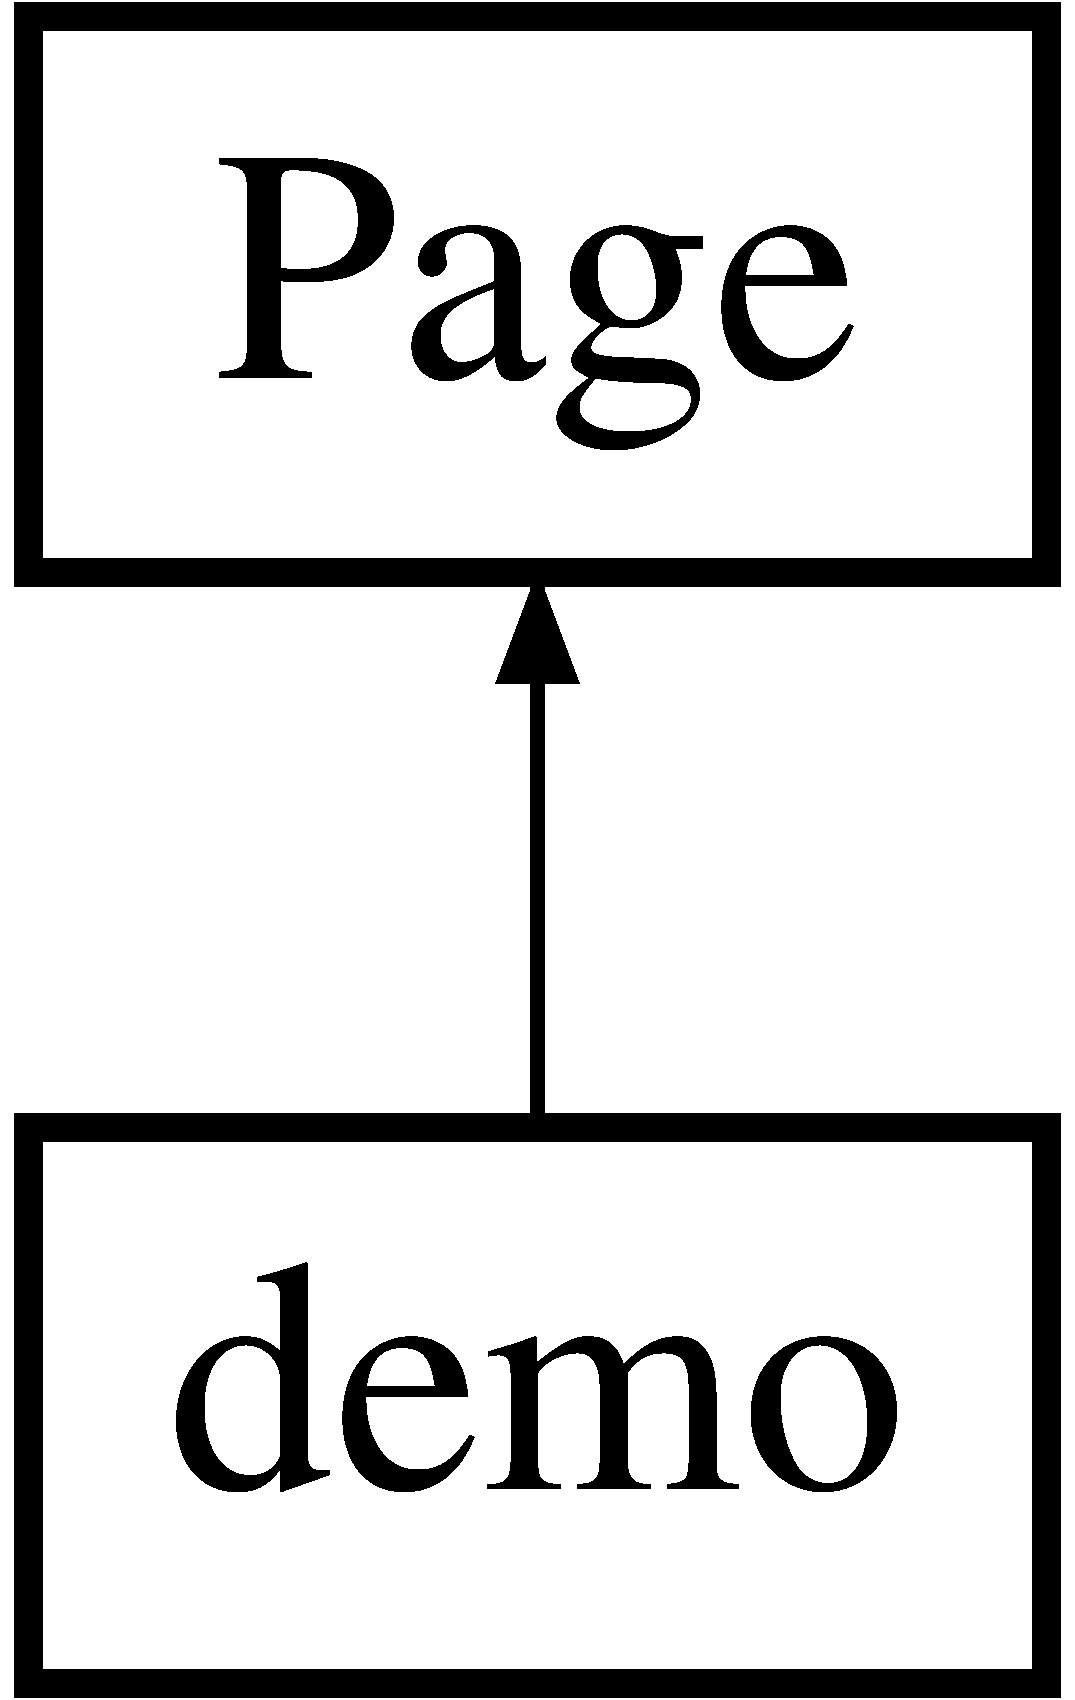
\includegraphics[height=2.000000cm]{classdemo}
\end{center}
\end{figure}
\subsection*{Protected Member Functions}
\begin{DoxyCompactItemize}
\item 
\hypertarget{classdemo_afa5fed50cf7d575d3b9984aaf31c9e8f}{void {\bfseries Page\-\_\-\-Load} (object sender, Event\-Args e)}\label{classdemo_afa5fed50cf7d575d3b9984aaf31c9e8f}

\end{DoxyCompactItemize}


\subsection{Detailed Description}


Definition at line 8 of file demo.\-aspx.\-cs.



The documentation for this class was generated from the following file\-:\begin{DoxyCompactItemize}
\item 
E\-:/\-Mint/\-Home care/\-Smart\-Home\-Care/demo.\-aspx.\-cs\end{DoxyCompactItemize}

\hypertarget{class_domain}{\section{Domain Class Reference}
\label{class_domain}\index{Domain@{Domain}}
}


create property  


\subsection*{Static Public Member Functions}
\begin{DoxyCompactItemize}
\item 
\hypertarget{class_domain_a7ad22ab73a4267af16f71e9add5e9eba}{static T {\bfseries Create$<$ T $>$} (string id, string name)}\label{class_domain_a7ad22ab73a4267af16f71e9add5e9eba}

\end{DoxyCompactItemize}


\subsection{Detailed Description}
create property 

Definition at line 94 of file Domain\-Object.\-cs.



The documentation for this class was generated from the following file\-:\begin{DoxyCompactItemize}
\item 
E\-:/\-Mint/\-Home care/\-Smart\-Home\-Care/\-App\-\_\-\-Code/Domain\-Object.\-cs\end{DoxyCompactItemize}

\hypertarget{class_domain_object}{\section{Domain\-Object Class Reference}
\label{class_domain_object}\index{Domain\-Object@{Domain\-Object}}
}


class build property  


Inheritance diagram for Domain\-Object\-:\begin{figure}[H]
\begin{center}
\leavevmode
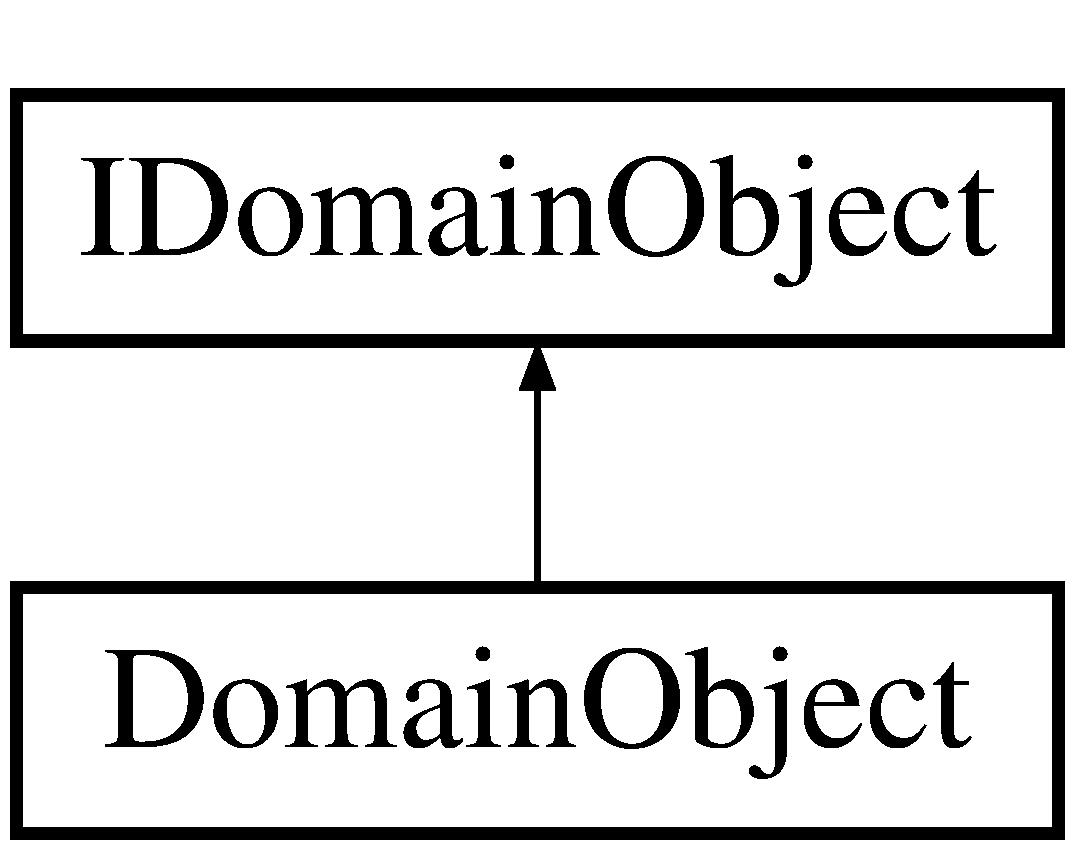
\includegraphics[height=2.000000cm]{class_domain_object}
\end{center}
\end{figure}
\subsection*{Public Member Functions}
\begin{DoxyCompactItemize}
\item 
\hypertarget{class_domain_object_aa2dfafd14a121be434d819465a22fc64}{\hyperlink{interface_i_data_record}{I\-Data\-Record} {\bfseries Create\-Data\-Record} ()}\label{class_domain_object_aa2dfafd14a121be434d819465a22fc64}

\end{DoxyCompactItemize}
\subsection*{Static Public Member Functions}
\begin{DoxyCompactItemize}
\item 
\hypertarget{class_domain_object_aa2e87aa051fb685f3baa5762afb6aa39}{static List$<$ T $>$ {\bfseries Combine$<$ T $>$} (params List$<$ T $>$\mbox{[}$\,$\mbox{]} objs)}\label{class_domain_object_aa2e87aa051fb685f3baa5762afb6aa39}

\item 
\hypertarget{class_domain_object_a62a97aee13e01adae000f6f8a09d8d5b}{static List$<$ T $>$ {\bfseries Intersect$<$ T $>$} (params List$<$ T $>$\mbox{[}$\,$\mbox{]} objs)}\label{class_domain_object_a62a97aee13e01adae000f6f8a09d8d5b}

\item 
\hypertarget{class_domain_object_ac3a86d7b35e19a67ff71c3817cd62765}{static List$<$ T $>$ {\bfseries Intersect\-Exclusive$<$ T $>$} (params List$<$ T $>$\mbox{[}$\,$\mbox{]} objs)}\label{class_domain_object_ac3a86d7b35e19a67ff71c3817cd62765}

\end{DoxyCompactItemize}
\subsection*{Properties}
\begin{DoxyCompactItemize}
\item 
\hypertarget{class_domain_object_aa3473b6ae65e61a547cdb676292e2786}{string {\bfseries Id}\hspace{0.3cm}{\ttfamily  \mbox{[}get, set\mbox{]}}}\label{class_domain_object_aa3473b6ae65e61a547cdb676292e2786}

\item 
\hypertarget{class_domain_object_a7e4a42db710b65918ff7937f8ed6f3f4}{string {\bfseries Name}\hspace{0.3cm}{\ttfamily  \mbox{[}get, set\mbox{]}}}\label{class_domain_object_a7e4a42db710b65918ff7937f8ed6f3f4}

\end{DoxyCompactItemize}


\subsection{Detailed Description}
class build property 

Definition at line 25 of file Domain\-Object.\-cs.



The documentation for this class was generated from the following file\-:\begin{DoxyCompactItemize}
\item 
E\-:/\-Mint/\-Home care/\-Smart\-Home\-Care/\-App\-\_\-\-Code/Domain\-Object.\-cs\end{DoxyCompactItemize}

\hypertarget{classforgotpassword}{\section{forgotpassword Class Reference}
\label{classforgotpassword}\index{forgotpassword@{forgotpassword}}
}
Inheritance diagram for forgotpassword\-:\begin{figure}[H]
\begin{center}
\leavevmode
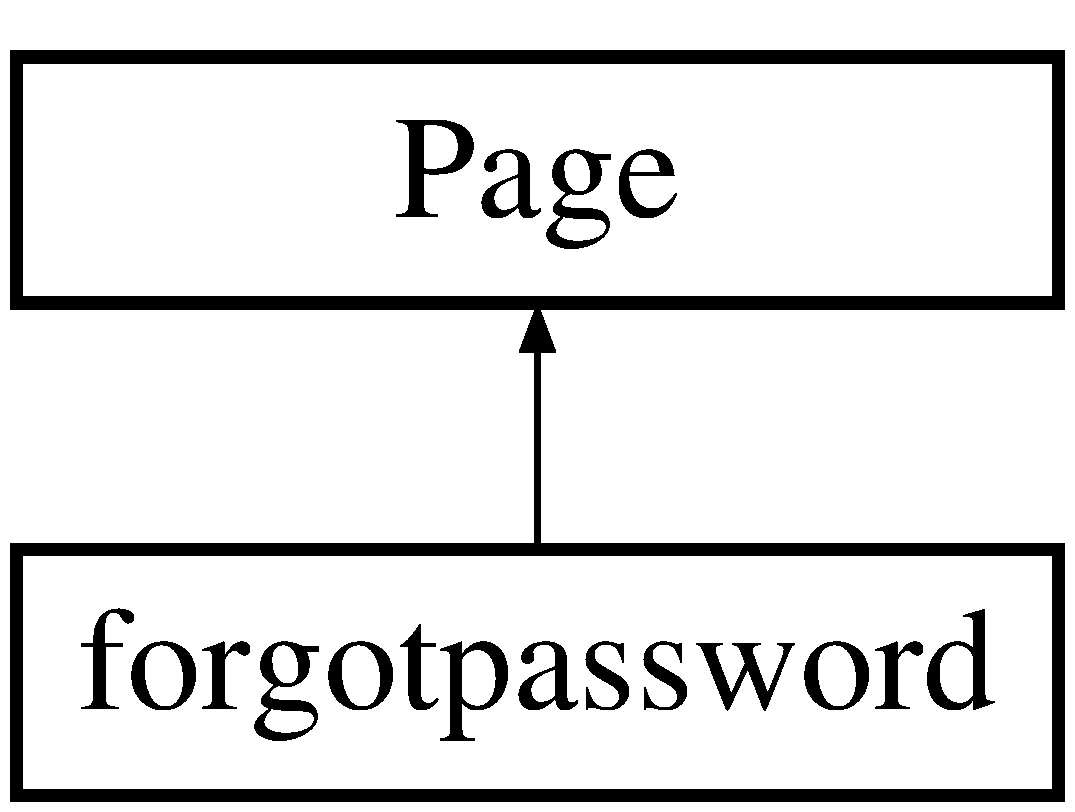
\includegraphics[height=2.000000cm]{classforgotpassword}
\end{center}
\end{figure}
\subsection*{Protected Member Functions}
\begin{DoxyCompactItemize}
\item 
\hypertarget{classforgotpassword_ad24f21574234e4235cdbfc0388977dd6}{void {\bfseries Page\-\_\-\-Load} (object sender, Event\-Args e)}\label{classforgotpassword_ad24f21574234e4235cdbfc0388977dd6}

\item 
\hypertarget{classforgotpassword_aa9f2786e5c66a11f5c9f1c26011e4bf3}{void {\bfseries btnsubmit\-\_\-\-Click} (object sender, Event\-Args e)}\label{classforgotpassword_aa9f2786e5c66a11f5c9f1c26011e4bf3}

\end{DoxyCompactItemize}


\subsection{Detailed Description}


Definition at line 9 of file forgotpassword.\-aspx.\-cs.



The documentation for this class was generated from the following file\-:\begin{DoxyCompactItemize}
\item 
E\-:/\-Mint/\-Home care/\-Smart\-Home\-Care/forgotpassword.\-aspx.\-cs\end{DoxyCompactItemize}

\hypertarget{classforgotusername}{\section{forgotusername Class Reference}
\label{classforgotusername}\index{forgotusername@{forgotusername}}
}
Inheritance diagram for forgotusername\-:\begin{figure}[H]
\begin{center}
\leavevmode
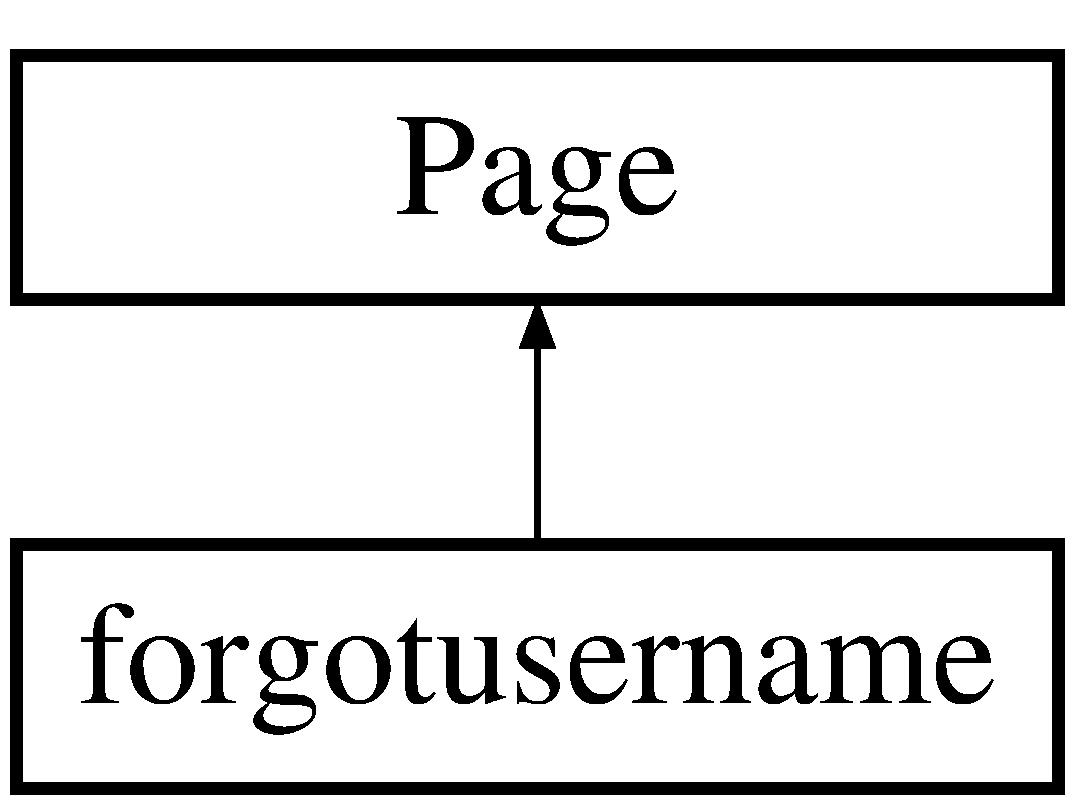
\includegraphics[height=2.000000cm]{classforgotusername}
\end{center}
\end{figure}
\subsection*{Protected Member Functions}
\begin{DoxyCompactItemize}
\item 
\hypertarget{classforgotusername_a7d92eb838d0a772f00ecd957480500bb}{void {\bfseries Page\-\_\-\-Load} (object sender, Event\-Args e)}\label{classforgotusername_a7d92eb838d0a772f00ecd957480500bb}

\item 
\hypertarget{classforgotusername_a5e5c45ac41c9ec60a2895cc1c7c2d3c4}{void {\bfseries btnsubmit\-\_\-\-Click} (object sender, Event\-Args e)}\label{classforgotusername_a5e5c45ac41c9ec60a2895cc1c7c2d3c4}

\end{DoxyCompactItemize}


\subsection{Detailed Description}


Definition at line 9 of file forgotusername.\-aspx.\-cs.



The documentation for this class was generated from the following file\-:\begin{DoxyCompactItemize}
\item 
E\-:/\-Mint/\-Home care/\-Smart\-Home\-Care/forgotusername.\-aspx.\-cs\end{DoxyCompactItemize}

\hypertarget{classfqas}{\section{fqas Class Reference}
\label{classfqas}\index{fqas@{fqas}}
}
Inheritance diagram for fqas\-:\begin{figure}[H]
\begin{center}
\leavevmode
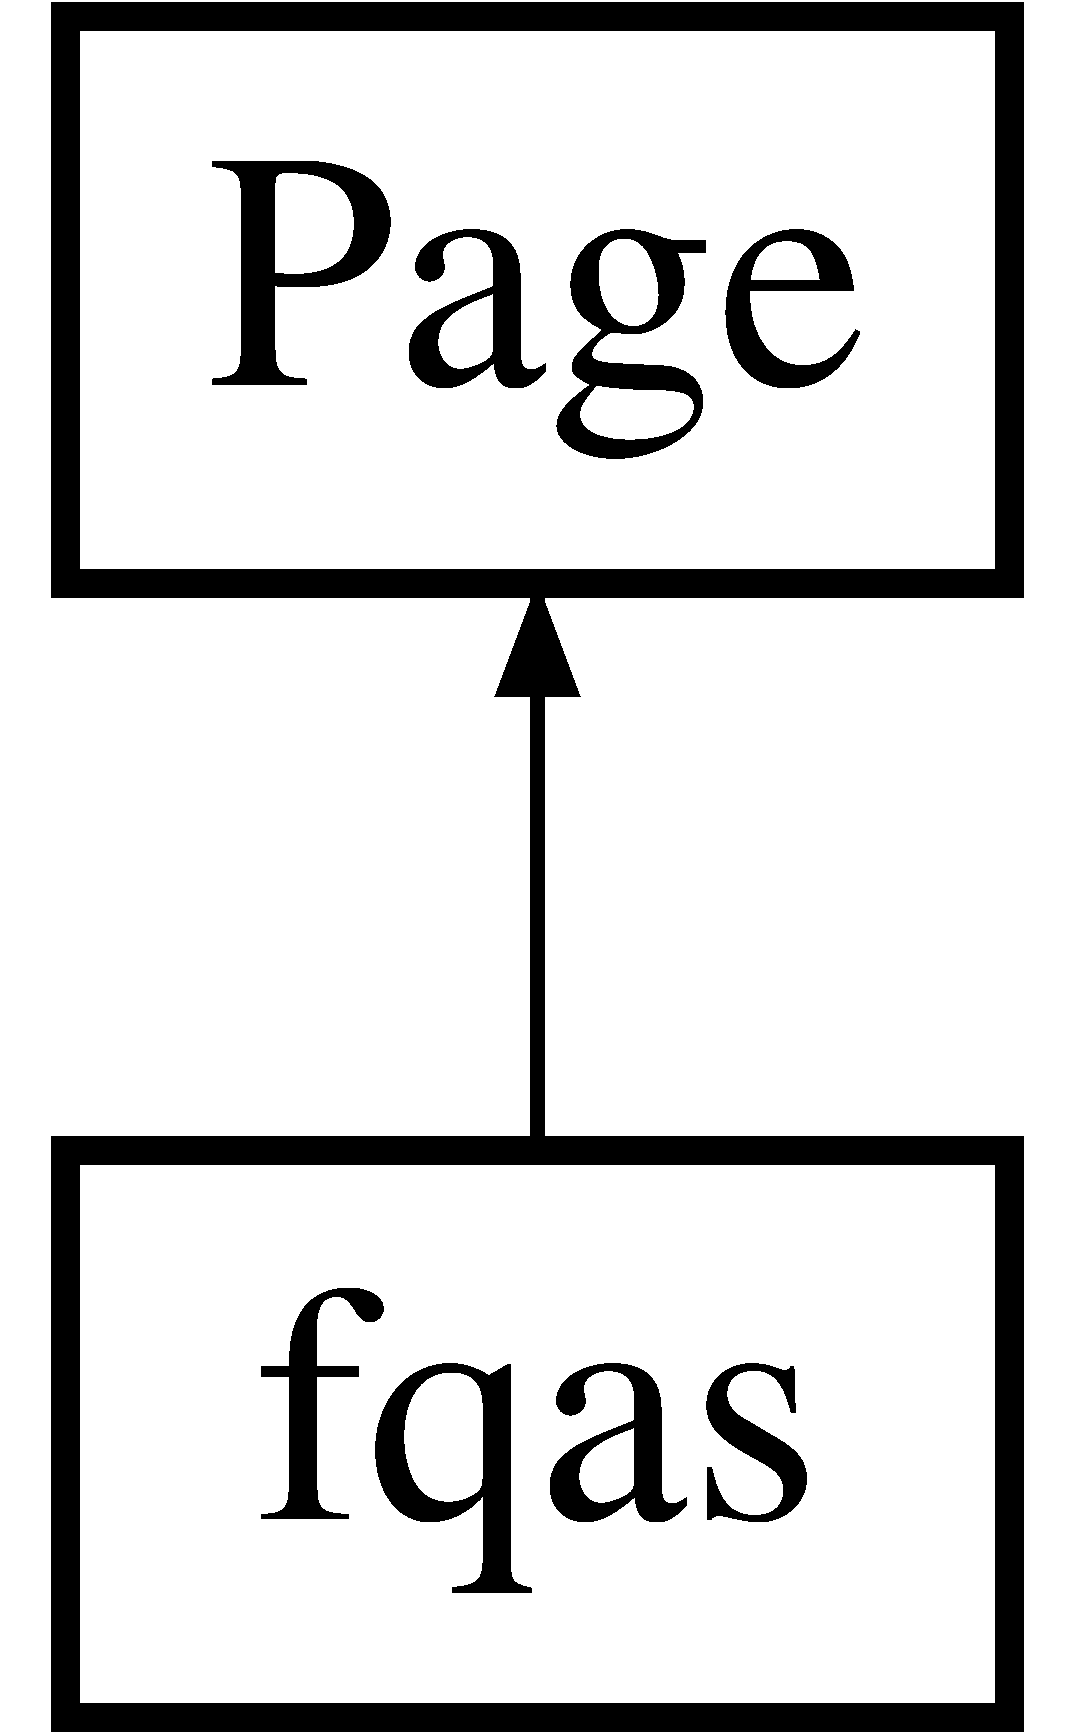
\includegraphics[height=2.000000cm]{classfqas}
\end{center}
\end{figure}
\subsection*{Protected Member Functions}
\begin{DoxyCompactItemize}
\item 
\hypertarget{classfqas_a3a30d3c05672631bcb1c14738086db45}{void {\bfseries Page\-\_\-\-Load} (object sender, Event\-Args e)}\label{classfqas_a3a30d3c05672631bcb1c14738086db45}

\end{DoxyCompactItemize}


\subsection{Detailed Description}


Definition at line 8 of file fqas.\-aspx.\-cs.



The documentation for this class was generated from the following file\-:\begin{DoxyCompactItemize}
\item 
E\-:/\-Mint/\-Home care/\-Smart\-Home\-Care/fqas.\-aspx.\-cs\end{DoxyCompactItemize}

\hypertarget{class_web_form_1_1_get_chart}{\section{Web\-Form.\-Get\-Chart Class Reference}
\label{class_web_form_1_1_get_chart}\index{Web\-Form.\-Get\-Chart@{Web\-Form.\-Get\-Chart}}
}


Summary description for \hyperlink{class_web_form_1_1_get_chart}{Get\-Chart}.  


Inheritance diagram for Web\-Form.\-Get\-Chart\-:\begin{figure}[H]
\begin{center}
\leavevmode
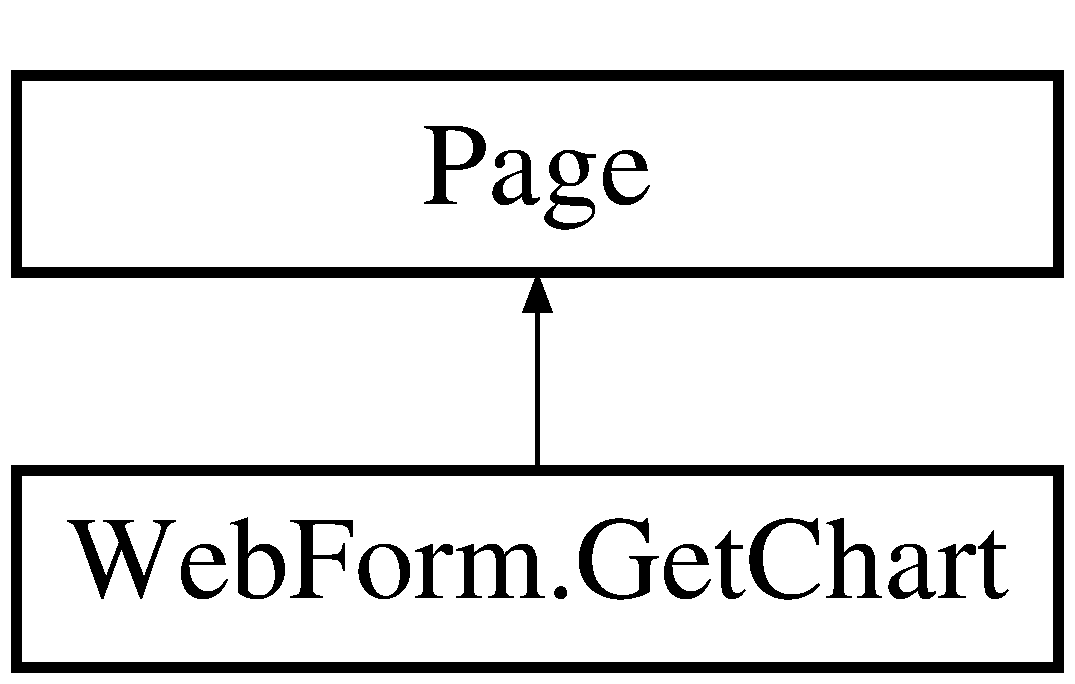
\includegraphics[height=2.000000cm]{class_web_form_1_1_get_chart}
\end{center}
\end{figure}
\subsection*{Protected Member Functions}
\begin{DoxyCompactItemize}
\item 
\hypertarget{class_web_form_1_1_get_chart_aed77cc171a1bed201a2de3eaee27d253}{void {\bfseries Page\-\_\-\-Load} (object sender, System.\-Event\-Args e)}\label{class_web_form_1_1_get_chart_aed77cc171a1bed201a2de3eaee27d253}

\item 
\hypertarget{class_web_form_1_1_get_chart_acb82a86b9d96cde0463edae04a877f03}{override void {\bfseries On\-Init} (Event\-Args e)}\label{class_web_form_1_1_get_chart_acb82a86b9d96cde0463edae04a877f03}

\end{DoxyCompactItemize}


\subsection{Detailed Description}
Summary description for \hyperlink{class_web_form_1_1_get_chart}{Get\-Chart}. 



Definition at line 19 of file Get\-Chart.\-aspx.\-cs.



The documentation for this class was generated from the following file\-:\begin{DoxyCompactItemize}
\item 
E\-:/\-Mint/\-Home care/\-Smart\-Home\-Care/Get\-Chart.\-aspx.\-cs\end{DoxyCompactItemize}

\hypertarget{classgotohome}{\section{gotohome Class Reference}
\label{classgotohome}\index{gotohome@{gotohome}}
}
Inheritance diagram for gotohome\-:\begin{figure}[H]
\begin{center}
\leavevmode
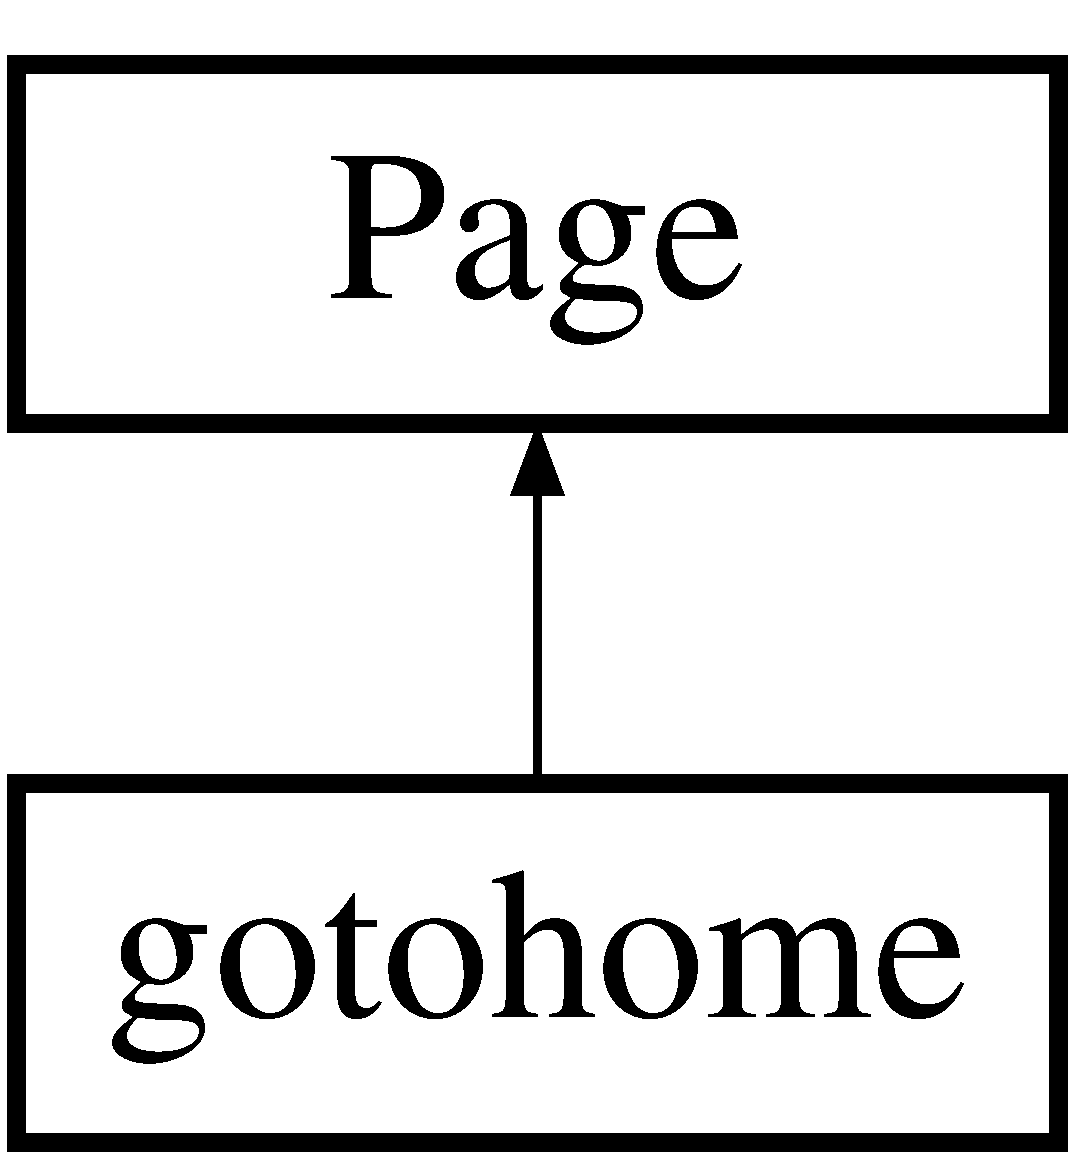
\includegraphics[height=2.000000cm]{classgotohome}
\end{center}
\end{figure}
\subsection*{Protected Member Functions}
\begin{DoxyCompactItemize}
\item 
\hypertarget{classgotohome_a16d750c3dd9dfe3208a39b2a8a5dea91}{void {\bfseries Page\-\_\-\-Load} (object sender, Event\-Args e)}\label{classgotohome_a16d750c3dd9dfe3208a39b2a8a5dea91}

\end{DoxyCompactItemize}


\subsection{Detailed Description}


Definition at line 8 of file gotohome.\-aspx.\-cs.



The documentation for this class was generated from the following file\-:\begin{DoxyCompactItemize}
\item 
E\-:/\-Mint/\-Home care/\-Smart\-Home\-Care/gotohome.\-aspx.\-cs\end{DoxyCompactItemize}

\hypertarget{classhome}{\section{home Class Reference}
\label{classhome}\index{home@{home}}
}
Inheritance diagram for home\-:\begin{figure}[H]
\begin{center}
\leavevmode
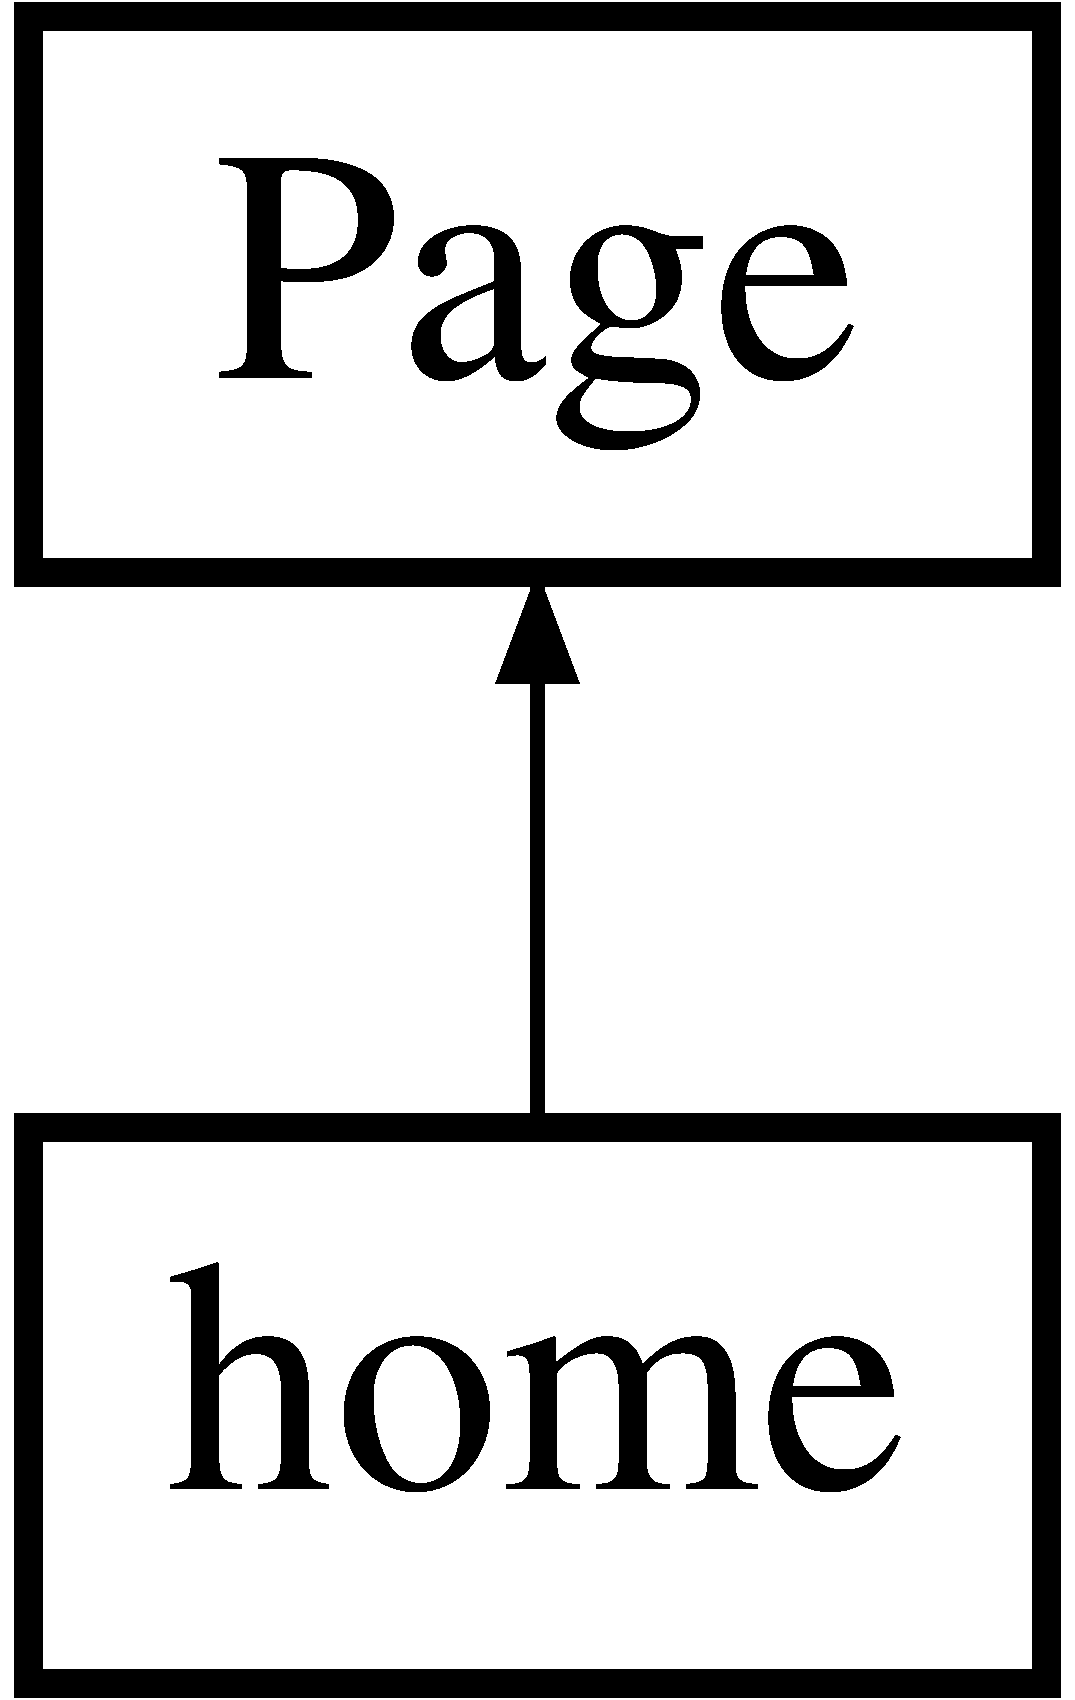
\includegraphics[height=2.000000cm]{classhome}
\end{center}
\end{figure}
\subsection*{Protected Member Functions}
\begin{DoxyCompactItemize}
\item 
void \hyperlink{classhome_a0966224aba2b7c5d1157a8383339db89}{Page\-\_\-\-Load} (object sender, Event\-Args e)
\begin{DoxyCompactList}\small\item\em Hàm để load trang. \end{DoxyCompactList}\item 
\hypertarget{classhome_aa077ce267f49a5b1fc42752b4007ea74}{void {\bfseries btnsignin\-\_\-\-Click} (object sender, Event\-Args e)}\label{classhome_aa077ce267f49a5b1fc42752b4007ea74}

\item 
\hypertarget{classhome_a929ab2b52ad63ed175a13bc34a874e87}{void {\bfseries lnkregister\-\_\-\-Click} (object sender, Event\-Args e)}\label{classhome_a929ab2b52ad63ed175a13bc34a874e87}

\item 
\hypertarget{classhome_a85a380d2567afa84fdb37a68056a0a61}{void {\bfseries lnkfqas\-\_\-\-Click} (object sender, Event\-Args e)}\label{classhome_a85a380d2567afa84fdb37a68056a0a61}

\item 
\hypertarget{classhome_a9956abd3ce21521d84ea29e4e49a43eb}{void {\bfseries lnkprivacypolicy\-\_\-\-Click} (object sender, Event\-Args e)}\label{classhome_a9956abd3ce21521d84ea29e4e49a43eb}

\item 
\hypertarget{classhome_ae67d0bc0a7ff45061f576208955efc00}{void {\bfseries lnktermsandconditions\-\_\-\-Click} (object sender, Event\-Args e)}\label{classhome_ae67d0bc0a7ff45061f576208955efc00}

\end{DoxyCompactItemize}


\subsection{Detailed Description}
Home class for login.

Class nay duoc su dung de làm gì đó ai mà biết 

Definition at line 15 of file home.\-aspx.\-cs.



\subsection{Member Function Documentation}
\hypertarget{classhome_a0966224aba2b7c5d1157a8383339db89}{\index{home@{home}!Page\-\_\-\-Load@{Page\-\_\-\-Load}}
\index{Page\-\_\-\-Load@{Page\-\_\-\-Load}!home@{home}}
\subsubsection[{Page\-\_\-\-Load}]{\setlength{\rightskip}{0pt plus 5cm}void home.\-Page\-\_\-\-Load (
\begin{DoxyParamCaption}
\item[{object}]{sender, }
\item[{Event\-Args}]{e}
\end{DoxyParamCaption}
)\hspace{0.3cm}{\ttfamily [protected]}}}\label{classhome_a0966224aba2b7c5d1157a8383339db89}


Hàm để load trang. 

Hàm này duoc su dung de load trang web. 
\begin{DoxyParams}{Parameters}
{\em sender} & la mot cai j do \\
\hline
{\em e} & la mot cai j khac nua \\
\hline
\end{DoxyParams}
\begin{DoxyReturn}{Returns}
la mot hai ba bon nam 
\end{DoxyReturn}
\begin{DoxySeeAlso}{See Also}
btnsignin\-\_\-\-Click() 
\end{DoxySeeAlso}


Definition at line 28 of file home.\-aspx.\-cs.



The documentation for this class was generated from the following file\-:\begin{DoxyCompactItemize}
\item 
E\-:/\-Mint/\-Home care/\-Smart\-Home\-Care/home.\-aspx.\-cs\end{DoxyCompactItemize}

\hypertarget{interface_i_data_record}{\section{I\-Data\-Record Interface Reference}
\label{interface_i_data_record}\index{I\-Data\-Record@{I\-Data\-Record}}
}


class interface of Data\-Record  




\subsection{Detailed Description}
class interface of Data\-Record 

Definition at line 9 of file Domain\-Object.\-cs.



The documentation for this interface was generated from the following file\-:\begin{DoxyCompactItemize}
\item 
E\-:/\-Mint/\-Home care/\-Smart\-Home\-Care/\-App\-\_\-\-Code/Domain\-Object.\-cs\end{DoxyCompactItemize}

\hypertarget{interface_i_domain_object}{\section{I\-Domain\-Object Interface Reference}
\label{interface_i_domain_object}\index{I\-Domain\-Object@{I\-Domain\-Object}}
}


class interface of \hyperlink{class_domain_object}{Domain\-Object}  


Inheritance diagram for I\-Domain\-Object\-:\begin{figure}[H]
\begin{center}
\leavevmode
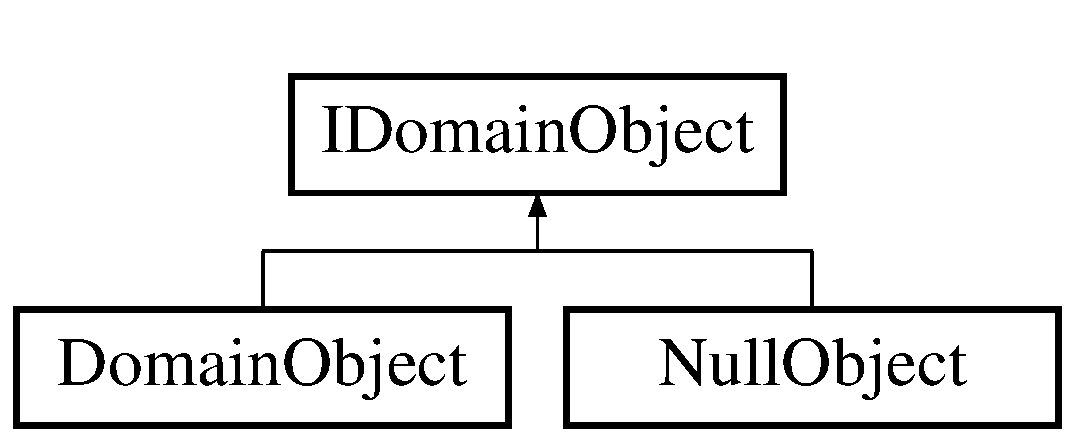
\includegraphics[height=2.000000cm]{interface_i_domain_object}
\end{center}
\end{figure}
\subsection*{Public Member Functions}
\begin{DoxyCompactItemize}
\item 
\hypertarget{interface_i_domain_object_acc9b6dc8f95dbfbb23fb152371ced472}{\hyperlink{interface_i_data_record}{I\-Data\-Record} {\bfseries Create\-Data\-Record} ()}\label{interface_i_domain_object_acc9b6dc8f95dbfbb23fb152371ced472}

\end{DoxyCompactItemize}
\subsection*{Properties}
\begin{DoxyCompactItemize}
\item 
\hypertarget{interface_i_domain_object_aee7b3c3e492a8faab64eda83cdb54841}{string {\bfseries Id}\hspace{0.3cm}{\ttfamily  \mbox{[}get, set\mbox{]}}}\label{interface_i_domain_object_aee7b3c3e492a8faab64eda83cdb54841}

\item 
\hypertarget{interface_i_domain_object_a2aa8f720dd778edd86bac7f4b09514d5}{string {\bfseries Name}\hspace{0.3cm}{\ttfamily  \mbox{[}get, set\mbox{]}}}\label{interface_i_domain_object_a2aa8f720dd778edd86bac7f4b09514d5}

\end{DoxyCompactItemize}


\subsection{Detailed Description}
class interface of \hyperlink{class_domain_object}{Domain\-Object} 

Definition at line 15 of file Domain\-Object.\-cs.



The documentation for this interface was generated from the following file\-:\begin{DoxyCompactItemize}
\item 
E\-:/\-Mint/\-Home care/\-Smart\-Home\-Care/\-App\-\_\-\-Code/Domain\-Object.\-cs\end{DoxyCompactItemize}

\hypertarget{classload_home_page}{\section{load\-Home\-Page Class Reference}
\label{classload_home_page}\index{load\-Home\-Page@{load\-Home\-Page}}
}
Inheritance diagram for load\-Home\-Page\-:\begin{figure}[H]
\begin{center}
\leavevmode
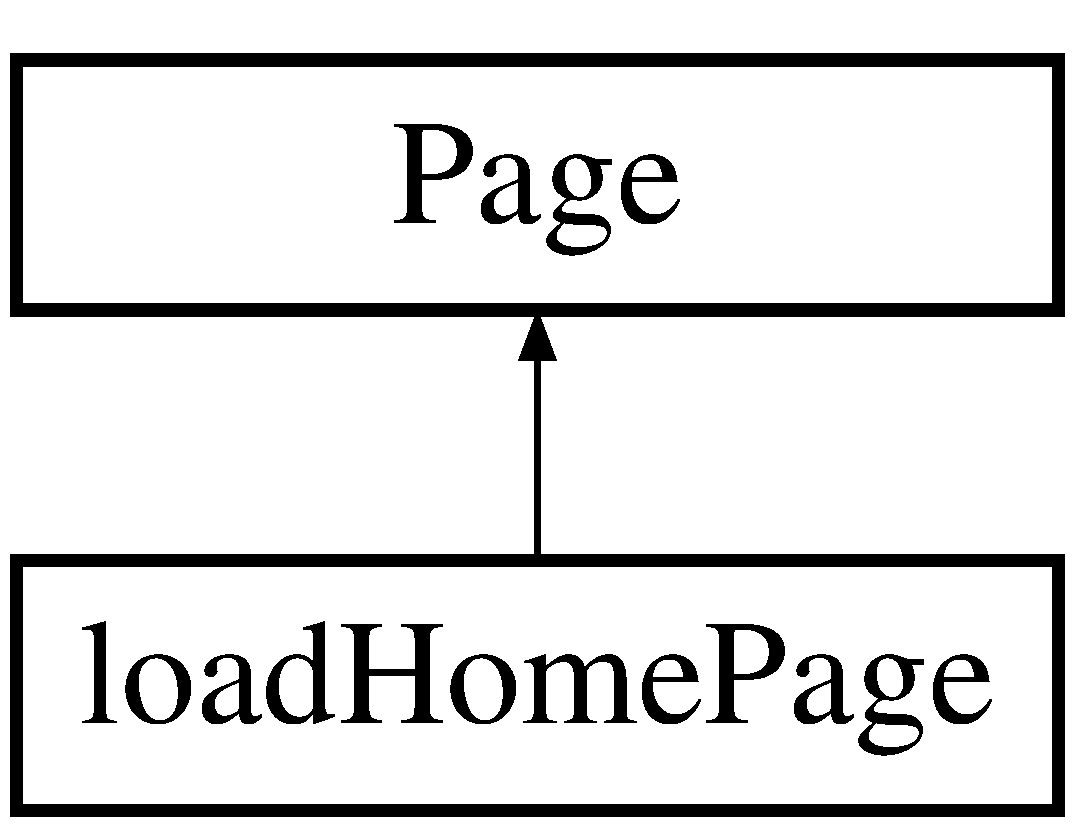
\includegraphics[height=2.000000cm]{classload_home_page}
\end{center}
\end{figure}
\subsection*{Protected Member Functions}
\begin{DoxyCompactItemize}
\item 
\hypertarget{classload_home_page_aa86ff482f8d3d2eb3cfc6fc9f2916d0e}{void {\bfseries Page\-\_\-\-Load} (object sender, Event\-Args e)}\label{classload_home_page_aa86ff482f8d3d2eb3cfc6fc9f2916d0e}

\end{DoxyCompactItemize}


\subsection{Detailed Description}


Definition at line 8 of file load\-Home\-Page.\-aspx.\-cs.



The documentation for this class was generated from the following file\-:\begin{DoxyCompactItemize}
\item 
E\-:/\-Mint/\-Home care/\-Smart\-Home\-Care/load\-Home\-Page.\-aspx.\-cs\end{DoxyCompactItemize}

\hypertarget{class_mail_daemon}{\section{Mail\-Daemon Class Reference}
\label{class_mail_daemon}\index{Mail\-Daemon@{Mail\-Daemon}}
}


process send mail  


\subsection*{Static Public Member Functions}
\begin{DoxyCompactItemize}
\item 
static void \hyperlink{class_mail_daemon_abd4af0c277915e06e5a238a6808212e9}{registration} (string email, string name, string webcode)
\item 
static void \hyperlink{class_mail_daemon_a5a855b66d82f24f1a49b3efca018d408}{forgotusername} (string email, string name, string username)
\item 
static void \hyperlink{class_mail_daemon_a5a6f07382cfdf3a38aa90b4e8bc282c5}{forgotpassword} (string email, string name, string passhint)
\item 
static void \hyperlink{class_mail_daemon_ae869b56204cb7ef5229acd5029f57c7e}{invitenewmember} (string email, string code, string name)
\end{DoxyCompactItemize}


\subsection{Detailed Description}
process send mail 

Definition at line 15 of file Mail\-Daemon.\-cs.



\subsection{Member Function Documentation}
\hypertarget{class_mail_daemon_a5a6f07382cfdf3a38aa90b4e8bc282c5}{\index{Mail\-Daemon@{Mail\-Daemon}!forgotpassword@{forgotpassword}}
\index{forgotpassword@{forgotpassword}!MailDaemon@{Mail\-Daemon}}
\subsubsection[{forgotpassword}]{\setlength{\rightskip}{0pt plus 5cm}static void Mail\-Daemon.\-forgotpassword (
\begin{DoxyParamCaption}
\item[{string}]{email, }
\item[{string}]{name, }
\item[{string}]{passhint}
\end{DoxyParamCaption}
)\hspace{0.3cm}{\ttfamily [static]}}}\label{class_mail_daemon_a5a6f07382cfdf3a38aa90b4e8bc282c5}
send mail, get back password \begin{DoxySeeAlso}{See Also}
\hyperlink{class_mail_daemon_a5a6f07382cfdf3a38aa90b4e8bc282c5}{forgotpassword()} 
\end{DoxySeeAlso}

\begin{DoxyParams}{Parameters}
{\em email} & is email account \\
\hline
{\em name} & is name account \\
\hline
{\em passhint} & sent mail \\
\hline
\end{DoxyParams}


Definition at line 300 of file Mail\-Daemon.\-cs.

\hypertarget{class_mail_daemon_a5a855b66d82f24f1a49b3efca018d408}{\index{Mail\-Daemon@{Mail\-Daemon}!forgotusername@{forgotusername}}
\index{forgotusername@{forgotusername}!MailDaemon@{Mail\-Daemon}}
\subsubsection[{forgotusername}]{\setlength{\rightskip}{0pt plus 5cm}static void Mail\-Daemon.\-forgotusername (
\begin{DoxyParamCaption}
\item[{string}]{email, }
\item[{string}]{name, }
\item[{string}]{username}
\end{DoxyParamCaption}
)\hspace{0.3cm}{\ttfamily [static]}}}\label{class_mail_daemon_a5a855b66d82f24f1a49b3efca018d408}
send mail, get back username \begin{DoxySeeAlso}{See Also}
\hyperlink{class_mail_daemon_a5a855b66d82f24f1a49b3efca018d408}{forgotusername()} 
\end{DoxySeeAlso}

\begin{DoxyParams}{Parameters}
{\em email} & is email account \\
\hline
{\em name} & is name account \\
\hline
{\em username} & sent mail \\
\hline
\end{DoxyParams}


Definition at line 254 of file Mail\-Daemon.\-cs.

\hypertarget{class_mail_daemon_ae869b56204cb7ef5229acd5029f57c7e}{\index{Mail\-Daemon@{Mail\-Daemon}!invitenewmember@{invitenewmember}}
\index{invitenewmember@{invitenewmember}!MailDaemon@{Mail\-Daemon}}
\subsubsection[{invitenewmember}]{\setlength{\rightskip}{0pt plus 5cm}static void Mail\-Daemon.\-invitenewmember (
\begin{DoxyParamCaption}
\item[{string}]{email, }
\item[{string}]{code, }
\item[{string}]{name}
\end{DoxyParamCaption}
)\hspace{0.3cm}{\ttfamily [static]}}}\label{class_mail_daemon_ae869b56204cb7ef5229acd5029f57c7e}
send mail, invite new member \begin{DoxySeeAlso}{See Also}
\hyperlink{class_mail_daemon_ae869b56204cb7ef5229acd5029f57c7e}{invitenewmember()} 
\end{DoxySeeAlso}

\begin{DoxyParams}{Parameters}
{\em email} & is invite \\
\hline
{\em code} & permission \\
\hline
{\em name} & is Invitations \\
\hline
\end{DoxyParams}


Definition at line 344 of file Mail\-Daemon.\-cs.

\hypertarget{class_mail_daemon_abd4af0c277915e06e5a238a6808212e9}{\index{Mail\-Daemon@{Mail\-Daemon}!registration@{registration}}
\index{registration@{registration}!MailDaemon@{Mail\-Daemon}}
\subsubsection[{registration}]{\setlength{\rightskip}{0pt plus 5cm}static void Mail\-Daemon.\-registration (
\begin{DoxyParamCaption}
\item[{string}]{email, }
\item[{string}]{name, }
\item[{string}]{webcode}
\end{DoxyParamCaption}
)\hspace{0.3cm}{\ttfamily [static]}}}\label{class_mail_daemon_abd4af0c277915e06e5a238a6808212e9}
send mail, enable registration \begin{DoxySeeAlso}{See Also}
\hyperlink{class_mail_daemon_abd4af0c277915e06e5a238a6808212e9}{registration()} 
\end{DoxySeeAlso}

\begin{DoxyParams}{Parameters}
{\em email} & is email registration \\
\hline
{\em name} & is name recipient \\
\hline
{\em webcode} & is enable account \\
\hline
\end{DoxyParams}


Definition at line 212 of file Mail\-Daemon.\-cs.



The documentation for this class was generated from the following file\-:\begin{DoxyCompactItemize}
\item 
E\-:/\-Mint/\-Home care/\-Smart\-Home\-Care/\-App\-\_\-\-Code/Mail\-Daemon.\-cs\end{DoxyCompactItemize}

\hypertarget{class_messages_box}{\section{Messages\-Box Class Reference}
\label{class_messages_box}\index{Messages\-Box@{Messages\-Box}}
}


messages box use for project  


\subsection*{Static Public Member Functions}
\begin{DoxyCompactItemize}
\item 
static void \hyperlink{class_messages_box_a957b15d12e12f117f8cbbc5b5ee081cc}{j\-Query\-Show} (Client\-Script\-Manager client\-Script, Type type, string Message, string title)
\item 
static void \hyperlink{class_messages_box_aa969029449da8c6ac0b1a22e8787ccfd}{Show} (string Message)
\end{DoxyCompactItemize}
\subsection*{Static Protected Attributes}
\begin{DoxyCompactItemize}
\item 
\hypertarget{class_messages_box_a5b4879c57ab2326d66cabc2568585322}{static Hashtable {\bfseries handler\-Pages} = new Hashtable()}\label{class_messages_box_a5b4879c57ab2326d66cabc2568585322}

\end{DoxyCompactItemize}


\subsection{Detailed Description}
messages box use for project 

Definition at line 13 of file Messages\-Box.\-cs.



\subsection{Member Function Documentation}
\hypertarget{class_messages_box_a957b15d12e12f117f8cbbc5b5ee081cc}{\index{Messages\-Box@{Messages\-Box}!j\-Query\-Show@{j\-Query\-Show}}
\index{j\-Query\-Show@{j\-Query\-Show}!MessagesBox@{Messages\-Box}}
\subsubsection[{j\-Query\-Show}]{\setlength{\rightskip}{0pt plus 5cm}static void Messages\-Box.\-j\-Query\-Show (
\begin{DoxyParamCaption}
\item[{Client\-Script\-Manager}]{client\-Script, }
\item[{Type}]{type, }
\item[{string}]{Message, }
\item[{string}]{title}
\end{DoxyParamCaption}
)\hspace{0.3cm}{\ttfamily [static]}}}\label{class_messages_box_a957b15d12e12f117f8cbbc5b5ee081cc}
\mbox{[}j\-Query\-Show\mbox{]} Show messages with jquery. 

Definition at line 24 of file Messages\-Box.\-cs.

\hypertarget{class_messages_box_aa969029449da8c6ac0b1a22e8787ccfd}{\index{Messages\-Box@{Messages\-Box}!Show@{Show}}
\index{Show@{Show}!MessagesBox@{Messages\-Box}}
\subsubsection[{Show}]{\setlength{\rightskip}{0pt plus 5cm}static void Messages\-Box.\-Show (
\begin{DoxyParamCaption}
\item[{string}]{Message}
\end{DoxyParamCaption}
)\hspace{0.3cm}{\ttfamily [static]}}}\label{class_messages_box_aa969029449da8c6ac0b1a22e8787ccfd}
\mbox{[}Messages Box Nomal\mbox{]} Show Messages box normal 

Definition at line 53 of file Messages\-Box.\-cs.



The documentation for this class was generated from the following file\-:\begin{DoxyCompactItemize}
\item 
E\-:/\-Mint/\-Home care/\-Smart\-Home\-Care/\-App\-\_\-\-Code/Messages\-Box.\-cs\end{DoxyCompactItemize}

\hypertarget{class_null_object}{\section{Null\-Object Class Reference}
\label{class_null_object}\index{Null\-Object@{Null\-Object}}
}


property default null  


Inheritance diagram for Null\-Object\-:\begin{figure}[H]
\begin{center}
\leavevmode
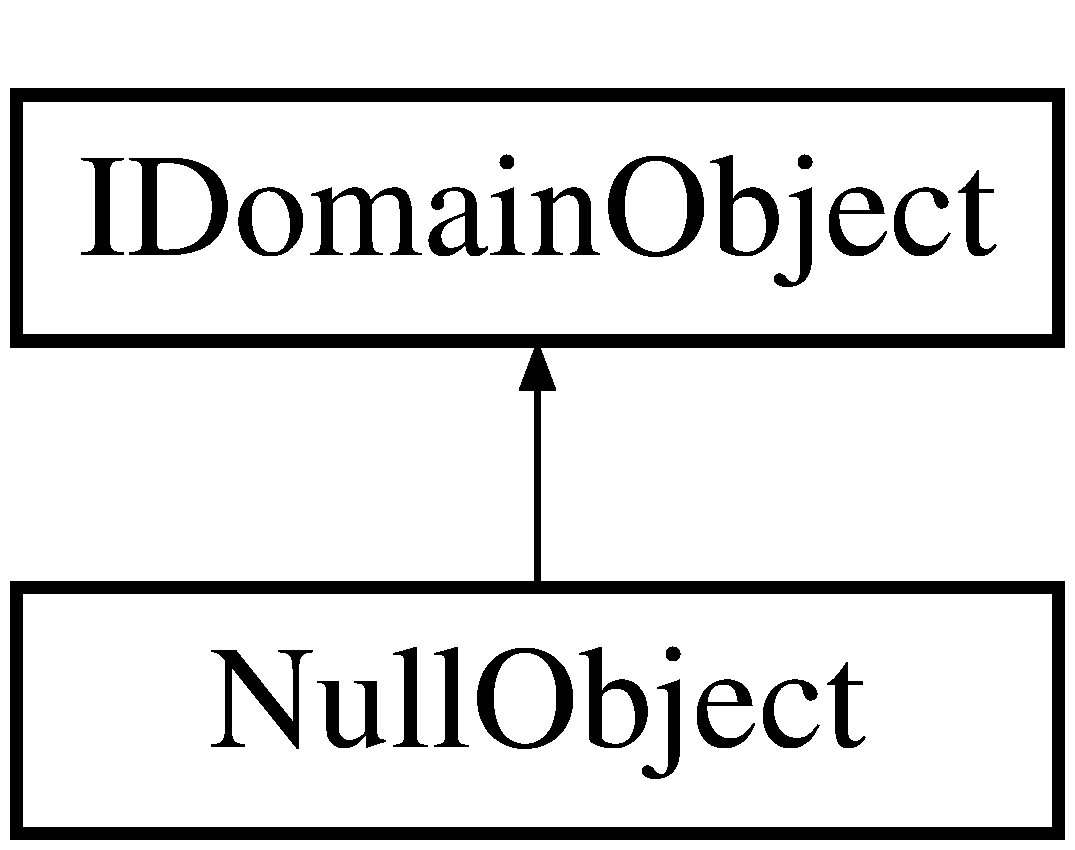
\includegraphics[height=2.000000cm]{class_null_object}
\end{center}
\end{figure}
\subsection*{Public Member Functions}
\begin{DoxyCompactItemize}
\item 
\hypertarget{class_null_object_a53244f0fed2420b39466d57a25f1e287}{\hyperlink{interface_i_data_record}{I\-Data\-Record} {\bfseries Create\-Data\-Record} ()}\label{class_null_object_a53244f0fed2420b39466d57a25f1e287}

\end{DoxyCompactItemize}
\subsection*{Properties}
\begin{DoxyCompactItemize}
\item 
\hypertarget{class_null_object_a0fa0dbed3423f426f1dc4a0d612e581a}{string {\bfseries Id}\hspace{0.3cm}{\ttfamily  \mbox{[}get, set\mbox{]}}}\label{class_null_object_a0fa0dbed3423f426f1dc4a0d612e581a}

\item 
\hypertarget{class_null_object_a59792d07ca1ea4d894cf64d0e0ef7d86}{string {\bfseries Name}\hspace{0.3cm}{\ttfamily  \mbox{[}get, set\mbox{]}}}\label{class_null_object_a59792d07ca1ea4d894cf64d0e0ef7d86}

\end{DoxyCompactItemize}


\subsection{Detailed Description}
property default null 

Definition at line 84 of file Domain\-Object.\-cs.



The documentation for this class was generated from the following file\-:\begin{DoxyCompactItemize}
\item 
E\-:/\-Mint/\-Home care/\-Smart\-Home\-Care/\-App\-\_\-\-Code/Domain\-Object.\-cs\end{DoxyCompactItemize}

\hypertarget{classpopup_date_time}{\section{popup\-Date\-Time Class Reference}
\label{classpopup_date_time}\index{popup\-Date\-Time@{popup\-Date\-Time}}
}
Inheritance diagram for popup\-Date\-Time\-:\begin{figure}[H]
\begin{center}
\leavevmode
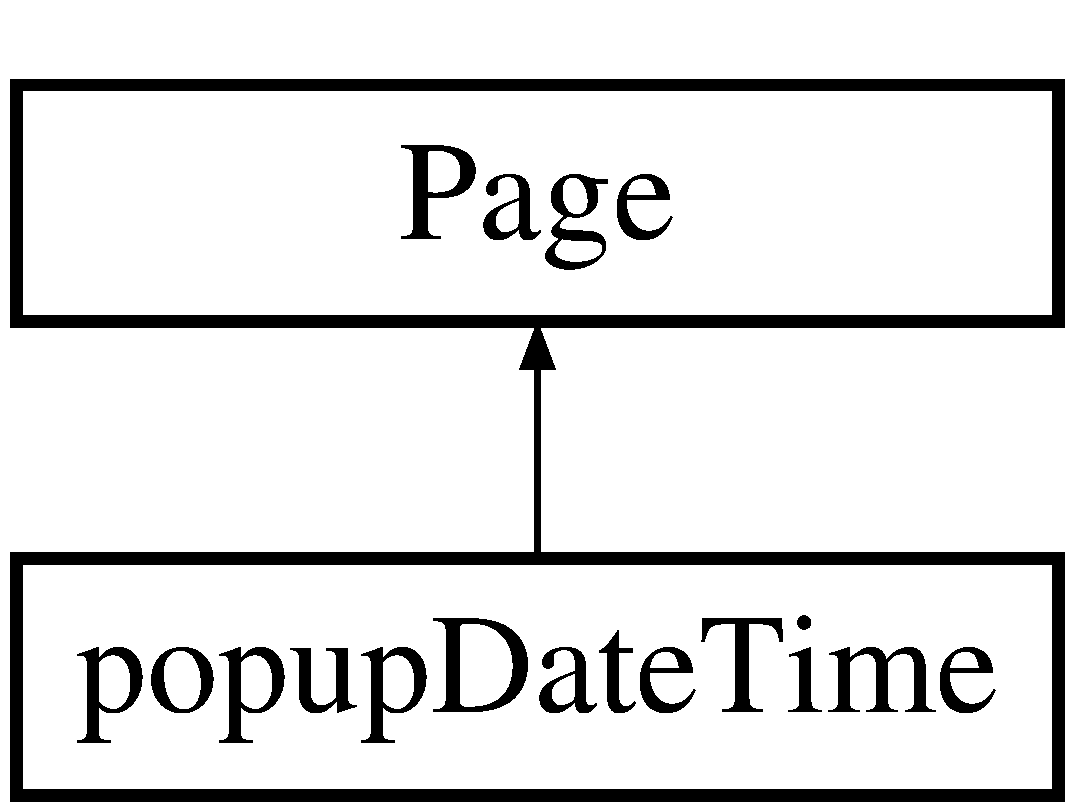
\includegraphics[height=2.000000cm]{classpopup_date_time}
\end{center}
\end{figure}
\subsection*{Protected Member Functions}
\begin{DoxyCompactItemize}
\item 
\hypertarget{classpopup_date_time_ae4a97a91b8649cbacfda1fcdd8e83ac1}{void {\bfseries Page\-\_\-\-Load} (object sender, Event\-Args e)}\label{classpopup_date_time_ae4a97a91b8649cbacfda1fcdd8e83ac1}

\end{DoxyCompactItemize}


\subsection{Detailed Description}


Definition at line 8 of file popup\-Date\-Time.\-aspx.\-cs.



The documentation for this class was generated from the following file\-:\begin{DoxyCompactItemize}
\item 
E\-:/\-Mint/\-Home care/\-Smart\-Home\-Care/popup\-Date\-Time.\-aspx.\-cs\end{DoxyCompactItemize}

\hypertarget{classprivacypolicy}{\section{privacypolicy Class Reference}
\label{classprivacypolicy}\index{privacypolicy@{privacypolicy}}
}
Inheritance diagram for privacypolicy\-:\begin{figure}[H]
\begin{center}
\leavevmode
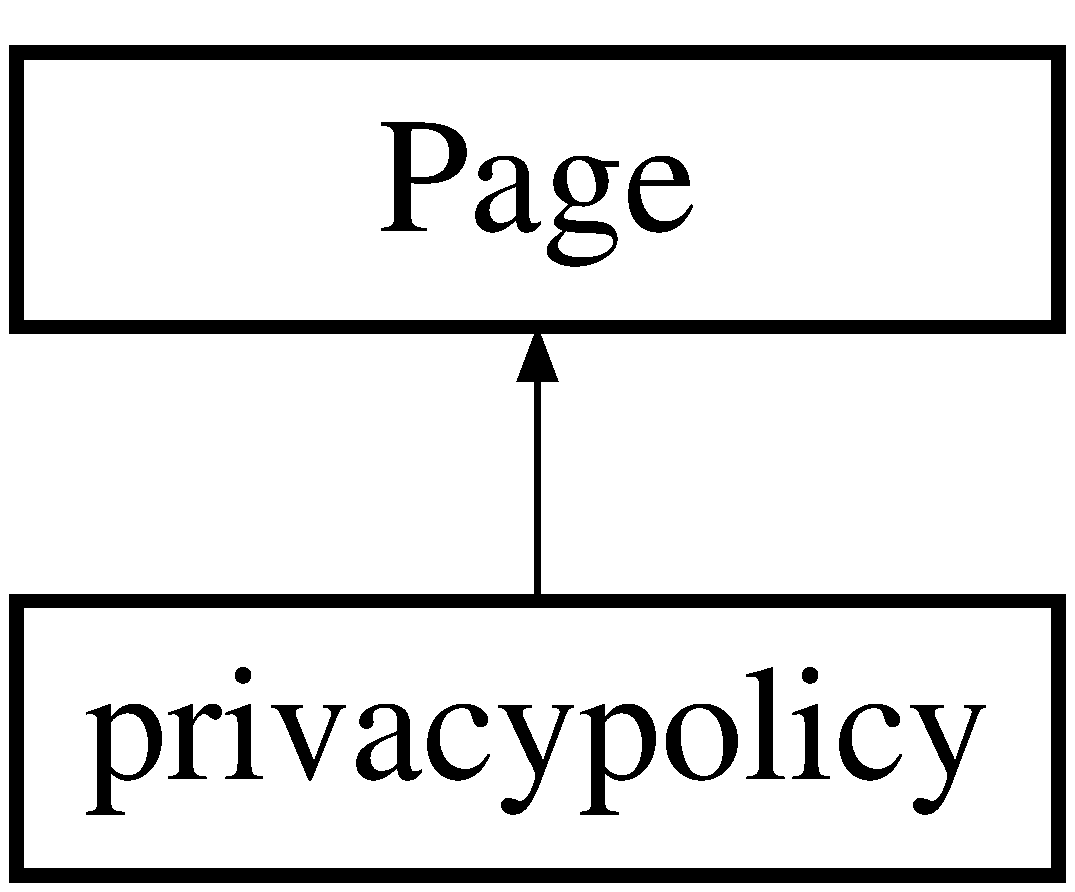
\includegraphics[height=2.000000cm]{classprivacypolicy}
\end{center}
\end{figure}
\subsection*{Protected Member Functions}
\begin{DoxyCompactItemize}
\item 
\hypertarget{classprivacypolicy_aaf46243bf8e6262178d1eaff5ba9b263}{void {\bfseries Page\-\_\-\-Load} (object sender, Event\-Args e)}\label{classprivacypolicy_aaf46243bf8e6262178d1eaff5ba9b263}

\end{DoxyCompactItemize}


\subsection{Detailed Description}


Definition at line 8 of file privacypolicy.\-aspx.\-cs.



The documentation for this class was generated from the following file\-:\begin{DoxyCompactItemize}
\item 
E\-:/\-Mint/\-Home care/\-Smart\-Home\-Care/privacypolicy.\-aspx.\-cs\end{DoxyCompactItemize}

\hypertarget{classregister}{\section{register Class Reference}
\label{classregister}\index{register@{register}}
}
Inheritance diagram for register\-:\begin{figure}[H]
\begin{center}
\leavevmode
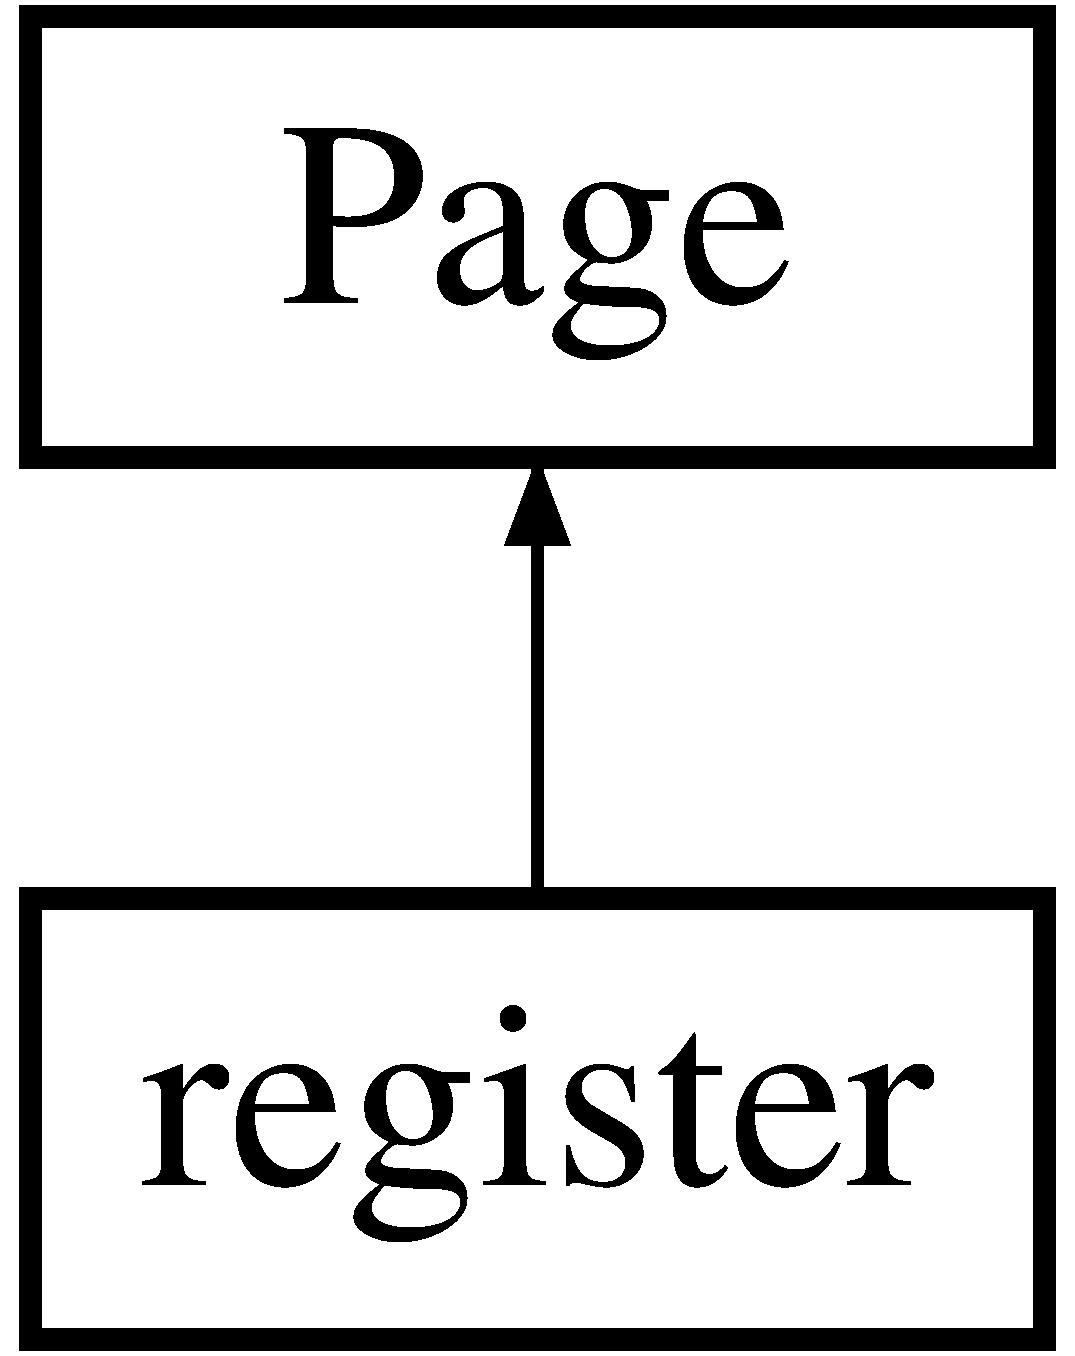
\includegraphics[height=2.000000cm]{classregister}
\end{center}
\end{figure}
\subsection*{Static Public Member Functions}
\begin{DoxyCompactItemize}
\item 
\hypertarget{classregister_a4f840630c47bf698b613359daf077c49}{static bool {\bfseries User\-Name\-Checker} (string username)}\label{classregister_a4f840630c47bf698b613359daf077c49}

\end{DoxyCompactItemize}
\subsection*{Protected Member Functions}
\begin{DoxyCompactItemize}
\item 
\hypertarget{classregister_ad970a9929fba7b42ad397e0340ee0e1c}{void {\bfseries Page\-\_\-\-Load} (object sender, Event\-Args e)}\label{classregister_ad970a9929fba7b42ad397e0340ee0e1c}

\item 
\hypertarget{classregister_a72797a079293dcb5e7c36c7827c1df28}{void {\bfseries btnregister\-\_\-\-Click} (object sender, Event\-Args e)}\label{classregister_a72797a079293dcb5e7c36c7827c1df28}

\item 
\hypertarget{classregister_a0bb326361d1b623d58b84a16dbc09c20}{void {\bfseries imgreload\-\_\-\-Click} (object sender, Image\-Click\-Event\-Args e)}\label{classregister_a0bb326361d1b623d58b84a16dbc09c20}

\item 
\hypertarget{classregister_a810466858f623a0f14a2f315fd72bf97}{void {\bfseries ddlcountry\-\_\-\-Selected\-Index\-Changed} (object sender, Event\-Args e)}\label{classregister_a810466858f623a0f14a2f315fd72bf97}

\item 
\hypertarget{classregister_a7dcda88483712ec46037d98673ffb125}{void {\bfseries btnaddmore\-\_\-\-Click} (object sender, Event\-Args e)}\label{classregister_a7dcda88483712ec46037d98673ffb125}

\item 
\hypertarget{classregister_a5d155a94e543c61f4d404d6f4b78ba5c}{override void {\bfseries On\-Load} (Event\-Args e)}\label{classregister_a5d155a94e543c61f4d404d6f4b78ba5c}

\end{DoxyCompactItemize}


\subsection{Detailed Description}


Definition at line 10 of file register.\-aspx.\-cs.



The documentation for this class was generated from the following file\-:\begin{DoxyCompactItemize}
\item 
E\-:/\-Mint/\-Home care/\-Smart\-Home\-Care/register.\-aspx.\-cs\end{DoxyCompactItemize}

\hypertarget{classregistersuccessfull}{\section{registersuccessfull Class Reference}
\label{classregistersuccessfull}\index{registersuccessfull@{registersuccessfull}}
}
Inheritance diagram for registersuccessfull\-:\begin{figure}[H]
\begin{center}
\leavevmode
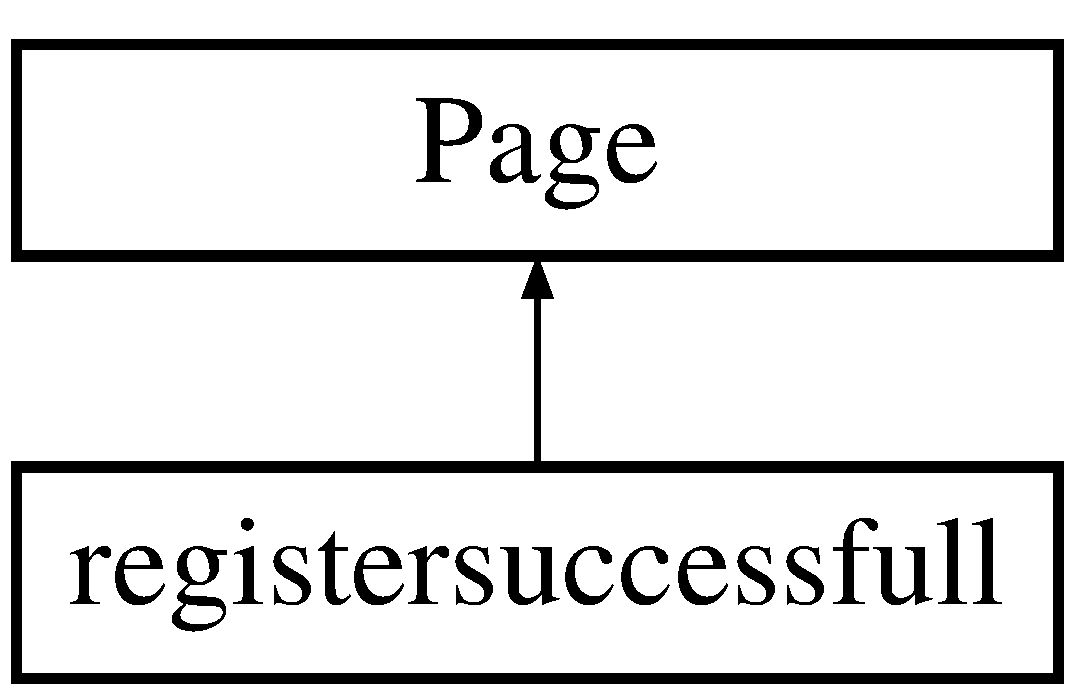
\includegraphics[height=2.000000cm]{classregistersuccessfull}
\end{center}
\end{figure}
\subsection*{Protected Member Functions}
\begin{DoxyCompactItemize}
\item 
\hypertarget{classregistersuccessfull_a0c36ad0fd253d47c27ebf267ad8fa010}{void {\bfseries Page\-\_\-\-Load} (object sender, Event\-Args e)}\label{classregistersuccessfull_a0c36ad0fd253d47c27ebf267ad8fa010}

\end{DoxyCompactItemize}


\subsection{Detailed Description}


Definition at line 8 of file registersuccessfull.\-aspx.\-cs.



The documentation for this class was generated from the following file\-:\begin{DoxyCompactItemize}
\item 
E\-:/\-Mint/\-Home care/\-Smart\-Home\-Care/registersuccessfull.\-aspx.\-cs\end{DoxyCompactItemize}

\hypertarget{class_security}{\section{Security Class Reference}
\label{class_security}\index{Security@{Security}}
}


all security method.  


\subsection*{Public Member Functions}
\begin{DoxyCompactItemize}
\item 
string \hyperlink{class_security_ad40bee17cc66f6bd636b891e570933c5}{Encrypt} (string key, string to\-Encrypt)
\item 
string \hyperlink{class_security_af503c53b350d8ff929fe71fac9ffab8e}{Decrypt} (string key, string to\-Decrypt)
\end{DoxyCompactItemize}
\subsection*{Static Public Member Functions}
\begin{DoxyCompactItemize}
\item 
static string \hyperlink{class_security_aadc3b8998851e010b4dd62cd46ebcd3c}{Get\-Version} ()
\item 
static string \hyperlink{class_security_a9395e3f676c1921278ed5a587c97ea72}{Generate\-Random\-Code} ()
\item 
static string \hyperlink{class_security_a7ccc2cb5ef5584b8e96fb4519a9e8750}{Get\-Client\-I\-P} ()
\item 
static string \hyperlink{class_security_ae23bcd950667cf41ec9f8ab924ed2ea6}{Get\-Server\-I\-P} ()
\end{DoxyCompactItemize}


\subsection{Detailed Description}
all security method. 

Definition at line 13 of file Security.\-cs.



\subsection{Member Function Documentation}
\hypertarget{class_security_af503c53b350d8ff929fe71fac9ffab8e}{\index{Security@{Security}!Decrypt@{Decrypt}}
\index{Decrypt@{Decrypt}!Security@{Security}}
\subsubsection[{Decrypt}]{\setlength{\rightskip}{0pt plus 5cm}string Security.\-Decrypt (
\begin{DoxyParamCaption}
\item[{string}]{key, }
\item[{string}]{to\-Decrypt}
\end{DoxyParamCaption}
)}}\label{class_security_af503c53b350d8ff929fe71fac9ffab8e}
Decrypt 1 string \begin{DoxySeeAlso}{See Also}
\hyperlink{class_security_af503c53b350d8ff929fe71fac9ffab8e}{Decrypt()} 
\end{DoxySeeAlso}

\begin{DoxyParams}{Parameters}
{\em key} & is key Decrypt \\
\hline
{\em to\-Encrypt} & is value Decrypt \\
\hline
\end{DoxyParams}


Definition at line 54 of file Security.\-cs.

\hypertarget{class_security_ad40bee17cc66f6bd636b891e570933c5}{\index{Security@{Security}!Encrypt@{Encrypt}}
\index{Encrypt@{Encrypt}!Security@{Security}}
\subsubsection[{Encrypt}]{\setlength{\rightskip}{0pt plus 5cm}string Security.\-Encrypt (
\begin{DoxyParamCaption}
\item[{string}]{key, }
\item[{string}]{to\-Encrypt}
\end{DoxyParamCaption}
)}}\label{class_security_ad40bee17cc66f6bd636b891e570933c5}
Encrypt 1 string \begin{DoxySeeAlso}{See Also}
\hyperlink{class_security_ad40bee17cc66f6bd636b891e570933c5}{Encrypt()} 
\end{DoxySeeAlso}

\begin{DoxyParams}{Parameters}
{\em key} & is key encrypt \\
\hline
{\em to\-Encrypt} & is value encrypt \\
\hline
\end{DoxyParams}


Definition at line 32 of file Security.\-cs.

\hypertarget{class_security_a9395e3f676c1921278ed5a587c97ea72}{\index{Security@{Security}!Generate\-Random\-Code@{Generate\-Random\-Code}}
\index{Generate\-Random\-Code@{Generate\-Random\-Code}!Security@{Security}}
\subsubsection[{Generate\-Random\-Code}]{\setlength{\rightskip}{0pt plus 5cm}static string Security.\-Generate\-Random\-Code (
\begin{DoxyParamCaption}
{}
\end{DoxyParamCaption}
)\hspace{0.3cm}{\ttfamily [static]}}}\label{class_security_a9395e3f676c1921278ed5a587c97ea72}
create 1 string random \begin{DoxySeeAlso}{See Also}
\hyperlink{class_security_a9395e3f676c1921278ed5a587c97ea72}{Generate\-Random\-Code()} 
\end{DoxySeeAlso}


Definition at line 75 of file Security.\-cs.

\hypertarget{class_security_a7ccc2cb5ef5584b8e96fb4519a9e8750}{\index{Security@{Security}!Get\-Client\-I\-P@{Get\-Client\-I\-P}}
\index{Get\-Client\-I\-P@{Get\-Client\-I\-P}!Security@{Security}}
\subsubsection[{Get\-Client\-I\-P}]{\setlength{\rightskip}{0pt plus 5cm}static string Security.\-Get\-Client\-I\-P (
\begin{DoxyParamCaption}
{}
\end{DoxyParamCaption}
)\hspace{0.3cm}{\ttfamily [static]}}}\label{class_security_a7ccc2cb5ef5584b8e96fb4519a9e8750}
get ip client(browser ip) \begin{DoxySeeAlso}{See Also}
\hyperlink{class_security_a7ccc2cb5ef5584b8e96fb4519a9e8750}{Get\-Client\-I\-P()} 
\end{DoxySeeAlso}


Definition at line 88 of file Security.\-cs.

\hypertarget{class_security_ae23bcd950667cf41ec9f8ab924ed2ea6}{\index{Security@{Security}!Get\-Server\-I\-P@{Get\-Server\-I\-P}}
\index{Get\-Server\-I\-P@{Get\-Server\-I\-P}!Security@{Security}}
\subsubsection[{Get\-Server\-I\-P}]{\setlength{\rightskip}{0pt plus 5cm}static string Security.\-Get\-Server\-I\-P (
\begin{DoxyParamCaption}
{}
\end{DoxyParamCaption}
)\hspace{0.3cm}{\ttfamily [static]}}}\label{class_security_ae23bcd950667cf41ec9f8ab924ed2ea6}
get ip server(local ip) \begin{DoxySeeAlso}{See Also}
\hyperlink{class_security_ae23bcd950667cf41ec9f8ab924ed2ea6}{Get\-Server\-I\-P()} 
\end{DoxySeeAlso}


Definition at line 98 of file Security.\-cs.

\hypertarget{class_security_aadc3b8998851e010b4dd62cd46ebcd3c}{\index{Security@{Security}!Get\-Version@{Get\-Version}}
\index{Get\-Version@{Get\-Version}!Security@{Security}}
\subsubsection[{Get\-Version}]{\setlength{\rightskip}{0pt plus 5cm}static string Security.\-Get\-Version (
\begin{DoxyParamCaption}
{}
\end{DoxyParamCaption}
)\hspace{0.3cm}{\ttfamily [static]}}}\label{class_security_aadc3b8998851e010b4dd62cd46ebcd3c}
Get version update 

Definition at line 22 of file Security.\-cs.



The documentation for this class was generated from the following file\-:\begin{DoxyCompactItemize}
\item 
E\-:/\-Mint/\-Home care/\-Smart\-Home\-Care/\-App\-\_\-\-Code/Security.\-cs\end{DoxyCompactItemize}

\hypertarget{class_service}{\section{Service Class Reference}
\label{class_service}\index{Service@{Service}}
}


convert data for webservice  


Inheritance diagram for Service\-:\begin{figure}[H]
\begin{center}
\leavevmode
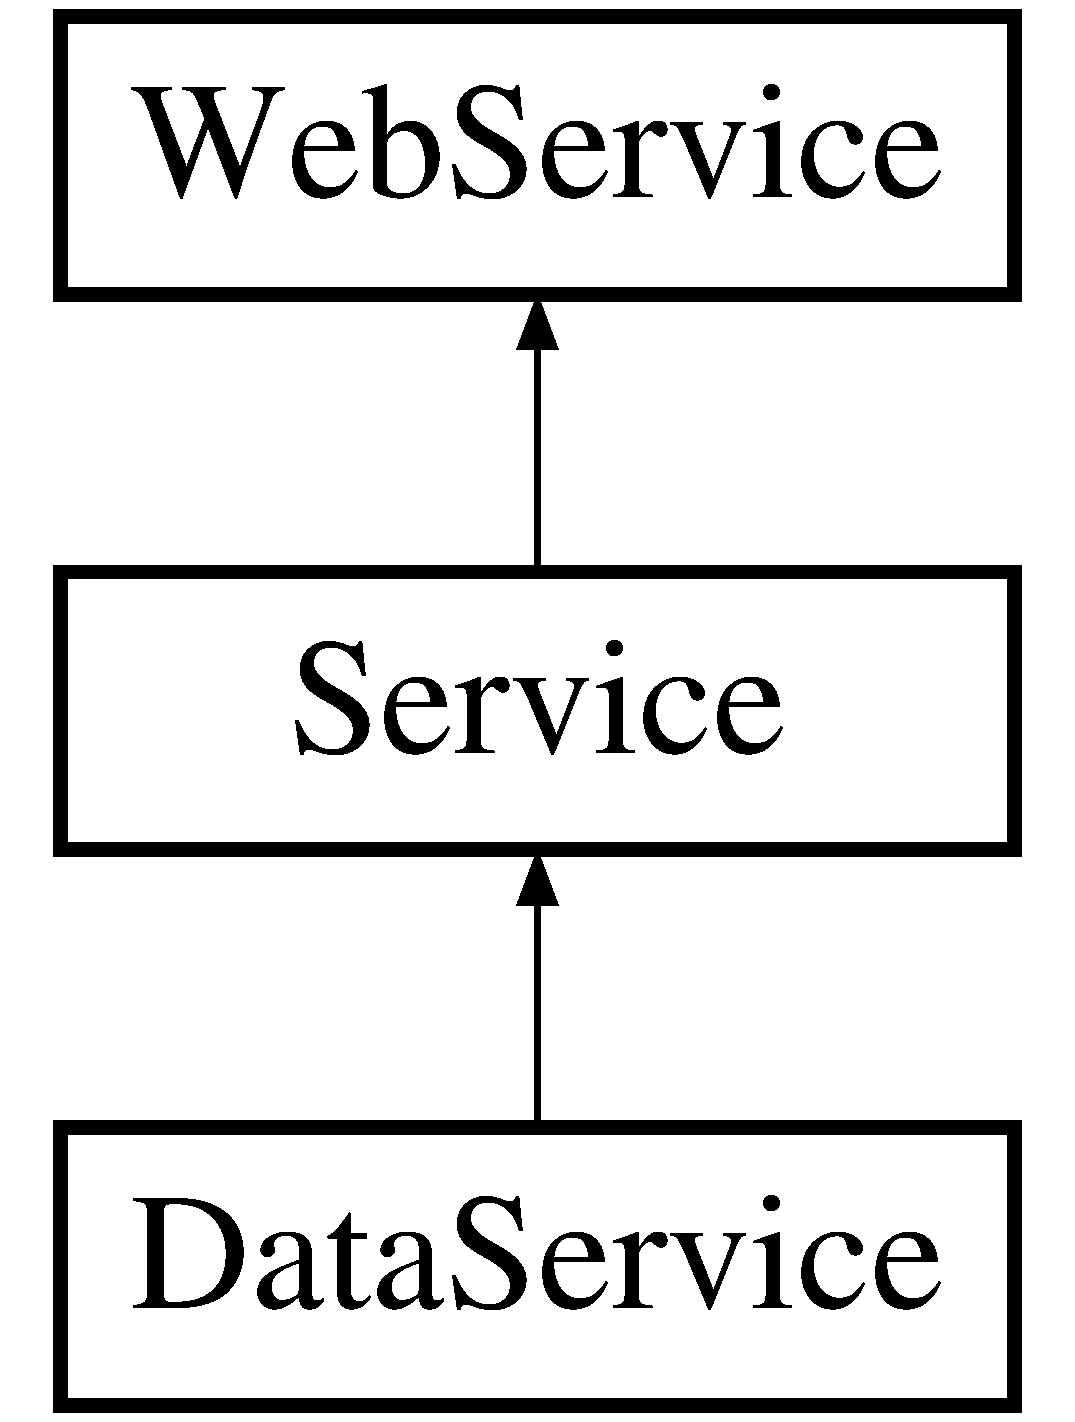
\includegraphics[height=3.000000cm]{class_service}
\end{center}
\end{figure}
\subsection*{Public Member Functions}
\begin{DoxyCompactItemize}
\item 
Xml\-Node \hyperlink{class_service_afd14865bdacaac0b84c2efea89320654}{Rename\-Node} (Xml\-Node node, string namespace\-U\-R\-I, string qualified\-Name)
\end{DoxyCompactItemize}
\subsection*{Static Public Member Functions}
\begin{DoxyCompactItemize}
\item 
static Xml\-Document \hyperlink{class_service_a6836ee15cfea9c0c97f5faefe540e190}{Create\-Serialized\-Object} (object obj)
\end{DoxyCompactItemize}
\subsection*{Protected Member Functions}
\begin{DoxyCompactItemize}
\item 
Xml\-Document \hyperlink{class_service_ab7266bcacaec5b4730d2cb7337b0353d}{Serialize\-Object} (object obj)
\item 
Xml\-Document \hyperlink{class_service_a5cbb22d24af1f69815d164fc8e4638b0}{Serialize\-Objects} (params object\mbox{[}$\,$\mbox{]} objs)
\item 
Xml\-Document \hyperlink{class_service_ae2b167bdde3ac6e6f69a29fbee3b56cd}{Add\-Object\-To\-Document} (Xml\-Document document, string node\-Name, object obj)
\end{DoxyCompactItemize}


\subsection{Detailed Description}
convert data for webservice 

Definition at line 11 of file Service.\-cs.



\subsection{Member Function Documentation}
\hypertarget{class_service_ae2b167bdde3ac6e6f69a29fbee3b56cd}{\index{Service@{Service}!Add\-Object\-To\-Document@{Add\-Object\-To\-Document}}
\index{Add\-Object\-To\-Document@{Add\-Object\-To\-Document}!Service@{Service}}
\subsubsection[{Add\-Object\-To\-Document}]{\setlength{\rightskip}{0pt plus 5cm}Xml\-Document Service.\-Add\-Object\-To\-Document (
\begin{DoxyParamCaption}
\item[{Xml\-Document}]{document, }
\item[{string}]{node\-Name, }
\item[{object}]{obj}
\end{DoxyParamCaption}
)\hspace{0.3cm}{\ttfamily [protected]}}}\label{class_service_ae2b167bdde3ac6e6f69a29fbee3b56cd}
add node to Xml\-Document \begin{DoxySeeAlso}{See Also}
\hyperlink{class_service_ae2b167bdde3ac6e6f69a29fbee3b56cd}{Add\-Object\-To\-Document()} 
\end{DoxySeeAlso}

\begin{DoxyParams}{Parameters}
{\em node\-Name} & is key node \\
\hline
{\em obj} & is value node \\
\hline
\end{DoxyParams}


Definition at line 97 of file Service.\-cs.

\hypertarget{class_service_a6836ee15cfea9c0c97f5faefe540e190}{\index{Service@{Service}!Create\-Serialized\-Object@{Create\-Serialized\-Object}}
\index{Create\-Serialized\-Object@{Create\-Serialized\-Object}!Service@{Service}}
\subsubsection[{Create\-Serialized\-Object}]{\setlength{\rightskip}{0pt plus 5cm}static Xml\-Document Service.\-Create\-Serialized\-Object (
\begin{DoxyParamCaption}
\item[{object}]{obj}
\end{DoxyParamCaption}
)\hspace{0.3cm}{\ttfamily [static]}}}\label{class_service_a6836ee15cfea9c0c97f5faefe540e190}
convert object to Xml\-Document \begin{DoxySeeAlso}{See Also}
\hyperlink{class_service_a6836ee15cfea9c0c97f5faefe540e190}{Create\-Serialized\-Object()} 
\end{DoxySeeAlso}


Definition at line 18 of file Service.\-cs.

\hypertarget{class_service_afd14865bdacaac0b84c2efea89320654}{\index{Service@{Service}!Rename\-Node@{Rename\-Node}}
\index{Rename\-Node@{Rename\-Node}!Service@{Service}}
\subsubsection[{Rename\-Node}]{\setlength{\rightskip}{0pt plus 5cm}Xml\-Node Service.\-Rename\-Node (
\begin{DoxyParamCaption}
\item[{Xml\-Node}]{node, }
\item[{string}]{namespace\-U\-R\-I, }
\item[{string}]{qualified\-Name}
\end{DoxyParamCaption}
)}}\label{class_service_afd14865bdacaac0b84c2efea89320654}
rename node of Xml\-Document \begin{DoxySeeAlso}{See Also}
\hyperlink{class_service_afd14865bdacaac0b84c2efea89320654}{Rename\-Node()} 
\end{DoxySeeAlso}

\begin{DoxyParams}{Parameters}
{\em node} & need rename \\
\hline
{\em qualified\-Name} & is value new node \\
\hline
\end{DoxyParams}


Definition at line 155 of file Service.\-cs.

\hypertarget{class_service_ab7266bcacaec5b4730d2cb7337b0353d}{\index{Service@{Service}!Serialize\-Object@{Serialize\-Object}}
\index{Serialize\-Object@{Serialize\-Object}!Service@{Service}}
\subsubsection[{Serialize\-Object}]{\setlength{\rightskip}{0pt plus 5cm}Xml\-Document Service.\-Serialize\-Object (
\begin{DoxyParamCaption}
\item[{object}]{obj}
\end{DoxyParamCaption}
)\hspace{0.3cm}{\ttfamily [protected]}}}\label{class_service_ab7266bcacaec5b4730d2cb7337b0353d}
convert object to Xml\-Document \begin{DoxySeeAlso}{See Also}
\hyperlink{class_service_ab7266bcacaec5b4730d2cb7337b0353d}{Serialize\-Object()} 
\end{DoxySeeAlso}


Definition at line 26 of file Service.\-cs.

\hypertarget{class_service_a5cbb22d24af1f69815d164fc8e4638b0}{\index{Service@{Service}!Serialize\-Objects@{Serialize\-Objects}}
\index{Serialize\-Objects@{Serialize\-Objects}!Service@{Service}}
\subsubsection[{Serialize\-Objects}]{\setlength{\rightskip}{0pt plus 5cm}Xml\-Document Service.\-Serialize\-Objects (
\begin{DoxyParamCaption}
\item[{params object\mbox{[}$\,$\mbox{]}}]{objs}
\end{DoxyParamCaption}
)\hspace{0.3cm}{\ttfamily [protected]}}}\label{class_service_a5cbb22d24af1f69815d164fc8e4638b0}
convert object array to Xml\-Document \begin{DoxySeeAlso}{See Also}
\hyperlink{class_service_a5cbb22d24af1f69815d164fc8e4638b0}{Serialize\-Objects()} 
\end{DoxySeeAlso}


Definition at line 34 of file Service.\-cs.



The documentation for this class was generated from the following file\-:\begin{DoxyCompactItemize}
\item 
E\-:/\-Mint/\-Home care/\-Smart\-Home\-Care/\-App\-\_\-\-Code/Service.\-cs\end{DoxyCompactItemize}

\hypertarget{classsite}{\section{site Class Reference}
\label{classsite}\index{site@{site}}
}
Inheritance diagram for site\-:\begin{figure}[H]
\begin{center}
\leavevmode
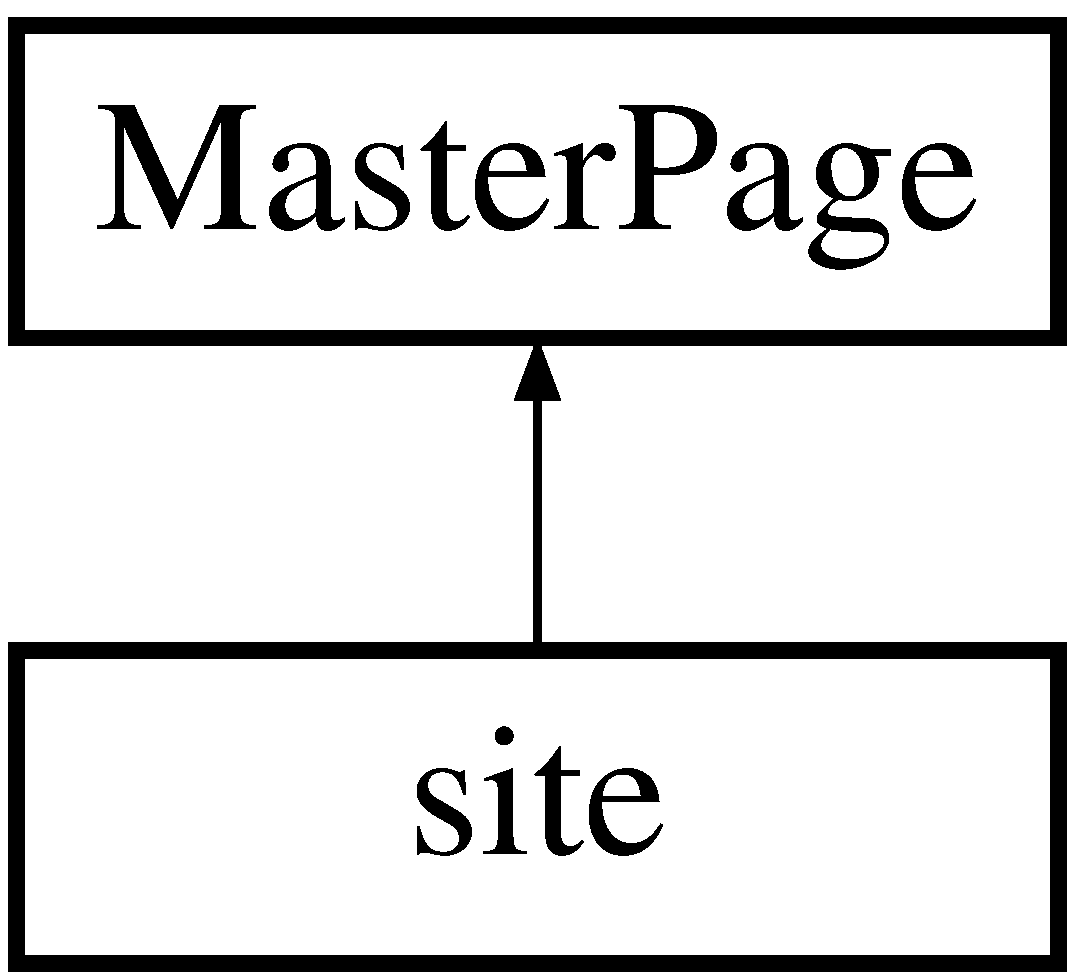
\includegraphics[height=2.000000cm]{classsite}
\end{center}
\end{figure}
\subsection*{Protected Member Functions}
\begin{DoxyCompactItemize}
\item 
\hypertarget{classsite_a91dce9b8a24da8fdecd43b16c218969d}{void {\bfseries Page\-\_\-\-Load} (object sender, Event\-Args e)}\label{classsite_a91dce9b8a24da8fdecd43b16c218969d}

\end{DoxyCompactItemize}


\subsection{Detailed Description}


Definition at line 9 of file site.\-master.\-cs.



The documentation for this class was generated from the following file\-:\begin{DoxyCompactItemize}
\item 
E\-:/\-Mint/\-Home care/\-Smart\-Home\-Care/site.\-master.\-cs\end{DoxyCompactItemize}

\hypertarget{classsiteadmin}{\section{siteadmin Class Reference}
\label{classsiteadmin}\index{siteadmin@{siteadmin}}
}
Inheritance diagram for siteadmin\-:\begin{figure}[H]
\begin{center}
\leavevmode
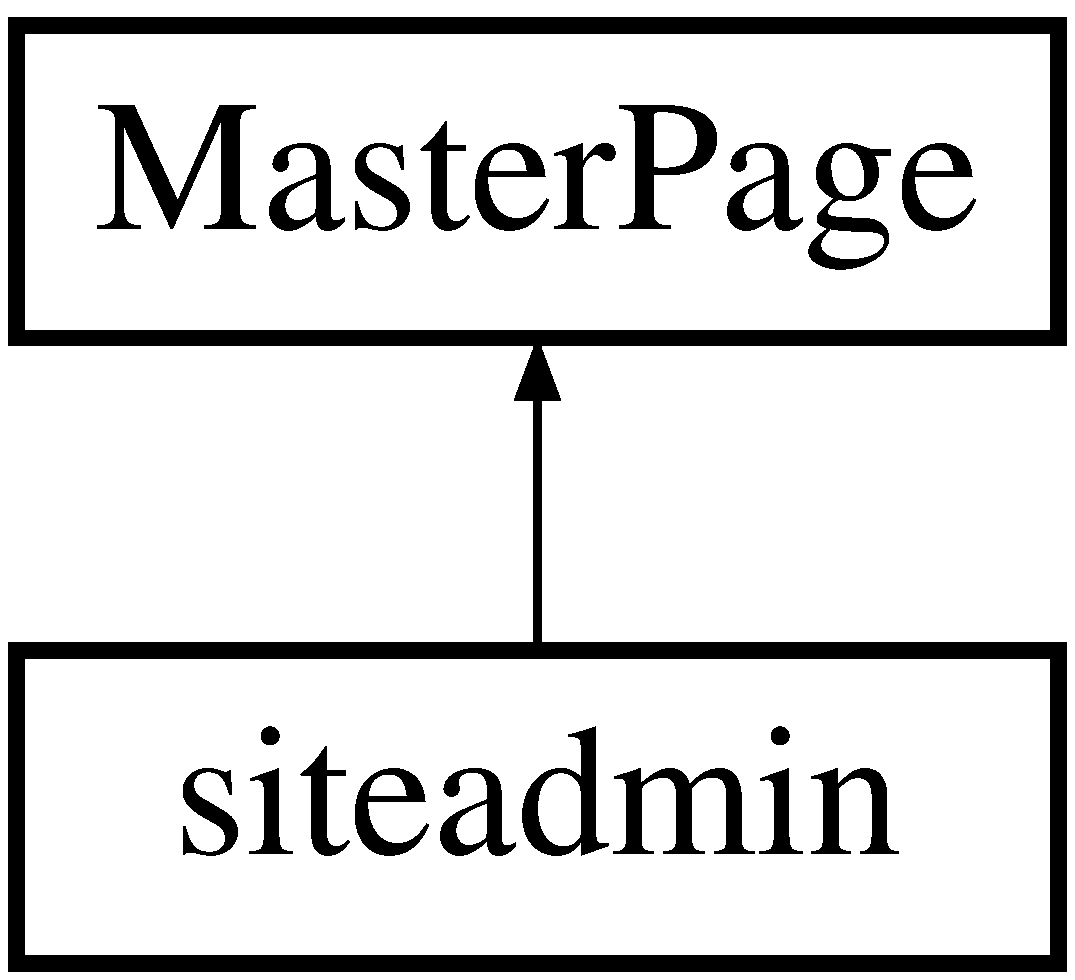
\includegraphics[height=2.000000cm]{classsiteadmin}
\end{center}
\end{figure}
\subsection*{Public Attributes}
\begin{DoxyCompactItemize}
\item 
\hypertarget{classsiteadmin_ac30faaa8f2cd36d9fc5e8a5dcd4937ff}{Tree\-View {\bfseries treeview}}\label{classsiteadmin_ac30faaa8f2cd36d9fc5e8a5dcd4937ff}

\item 
\hypertarget{classsiteadmin_a61fdc6987b79b4abe37f915bbe1f4134}{const int {\bfseries U\-S\-E\-R\-M\-A\-N\-A\-G\-E\-M\-E\-N\-T} = 0}\label{classsiteadmin_a61fdc6987b79b4abe37f915bbe1f4134}

\item 
\hypertarget{classsiteadmin_a918138b28499fd11cab61cabff9045e8}{const int {\bfseries R\-E\-P\-O\-R\-T\-S} = 1}\label{classsiteadmin_a918138b28499fd11cab61cabff9045e8}

\item 
\hypertarget{classsiteadmin_a58763ad9654a9eecf2419da457d1a420}{const int {\bfseries L\-O\-G\-S} = 2}\label{classsiteadmin_a58763ad9654a9eecf2419da457d1a420}

\item 
\hypertarget{classsiteadmin_a641e97f38db6ecadb701d0b5ee8a1548}{const int {\bfseries S\-Y\-S\-T\-E\-M\-T\-O\-O\-L\-S} = 3}\label{classsiteadmin_a641e97f38db6ecadb701d0b5ee8a1548}

\item 
\hypertarget{classsiteadmin_a5f210a5596361c3c0881848082890fc2}{const int {\bfseries M\-E\-S\-S\-A\-G\-E\-C\-E\-N\-T\-E\-R} = 4}\label{classsiteadmin_a5f210a5596361c3c0881848082890fc2}

\item 
\hypertarget{classsiteadmin_ab1f95c89ad33efe123e3f08a67e2c952}{const int {\bfseries M\-Y\-A\-C\-C\-O\-U\-N\-T} = 5}\label{classsiteadmin_ab1f95c89ad33efe123e3f08a67e2c952}

\item 
\hypertarget{classsiteadmin_a5b5d98c237beaad7f1b0dcdcf42d3e85}{const int {\bfseries S\-T\-A\-T\-I\-S\-T\-I\-C\-S} = 0}\label{classsiteadmin_a5b5d98c237beaad7f1b0dcdcf42d3e85}

\item 
\hypertarget{classsiteadmin_a06f7343e095e89bd5bdad54b494337d0}{const int {\bfseries W\-E\-B\-A\-D\-M\-I\-N\-L\-O\-G\-S} = 0}\label{classsiteadmin_a06f7343e095e89bd5bdad54b494337d0}

\item 
\hypertarget{classsiteadmin_a79b46c56b830dc2193f285d0fccd5801}{const int {\bfseries S\-Y\-N\-C\-L\-O\-G} = 1}\label{classsiteadmin_a79b46c56b830dc2193f285d0fccd5801}

\item 
\hypertarget{classsiteadmin_a85450122969cdfad519bee71563fbf75}{const int {\bfseries S\-E\-C\-U\-R\-I\-T\-Y} = 0}\label{classsiteadmin_a85450122969cdfad519bee71563fbf75}

\item 
\hypertarget{classsiteadmin_ab1897f2ca6c9fc6c85d3e0f53bb95622}{const int {\bfseries C\-O\-N\-F\-I\-G\-U\-R\-E} = 1}\label{classsiteadmin_ab1897f2ca6c9fc6c85d3e0f53bb95622}

\item 
\hypertarget{classsiteadmin_a3e1e569a5a86ecb0ed6f01b8fb529219}{const int {\bfseries I\-N\-B\-O\-X} = 1}\label{classsiteadmin_a3e1e569a5a86ecb0ed6f01b8fb529219}

\item 
\hypertarget{classsiteadmin_a608eb6bff3a2afa7469e2923f27976a4}{const int {\bfseries C\-O\-M\-P\-O\-S\-E} = 0}\label{classsiteadmin_a608eb6bff3a2afa7469e2923f27976a4}

\item 
\hypertarget{classsiteadmin_a607040133edce9c856a173d4d11038eb}{const int {\bfseries S\-E\-N\-T\-M\-E\-S\-S\-A\-G\-E\-S} = 2}\label{classsiteadmin_a607040133edce9c856a173d4d11038eb}

\item 
\hypertarget{classsiteadmin_a52cd2fb7538e06f9bd3309eb3fdf3843}{const int {\bfseries T\-R\-A\-S\-H} = 3}\label{classsiteadmin_a52cd2fb7538e06f9bd3309eb3fdf3843}

\end{DoxyCompactItemize}
\subsection*{Protected Member Functions}
\begin{DoxyCompactItemize}
\item 
\hypertarget{classsiteadmin_aff7f38e8dcd84e3c31fc6dd7cf2e5e22}{void {\bfseries Page\-\_\-\-Init} (object sender, Event\-Args e)}\label{classsiteadmin_aff7f38e8dcd84e3c31fc6dd7cf2e5e22}

\item 
\hypertarget{classsiteadmin_a57862374666f9bb2bf16c5b5683b24a3}{void {\bfseries Page\-\_\-\-Load} (object sender, Event\-Args e)}\label{classsiteadmin_a57862374666f9bb2bf16c5b5683b24a3}

\end{DoxyCompactItemize}


\subsection{Detailed Description}


Definition at line 9 of file siteadmin.\-master.\-cs.



The documentation for this class was generated from the following file\-:\begin{DoxyCompactItemize}
\item 
E\-:/\-Mint/\-Home care/\-Smart\-Home\-Care/siteadmin.\-master.\-cs\end{DoxyCompactItemize}

\hypertarget{classsitehome}{\section{sitehome Class Reference}
\label{classsitehome}\index{sitehome@{sitehome}}
}
Inheritance diagram for sitehome\-:\begin{figure}[H]
\begin{center}
\leavevmode
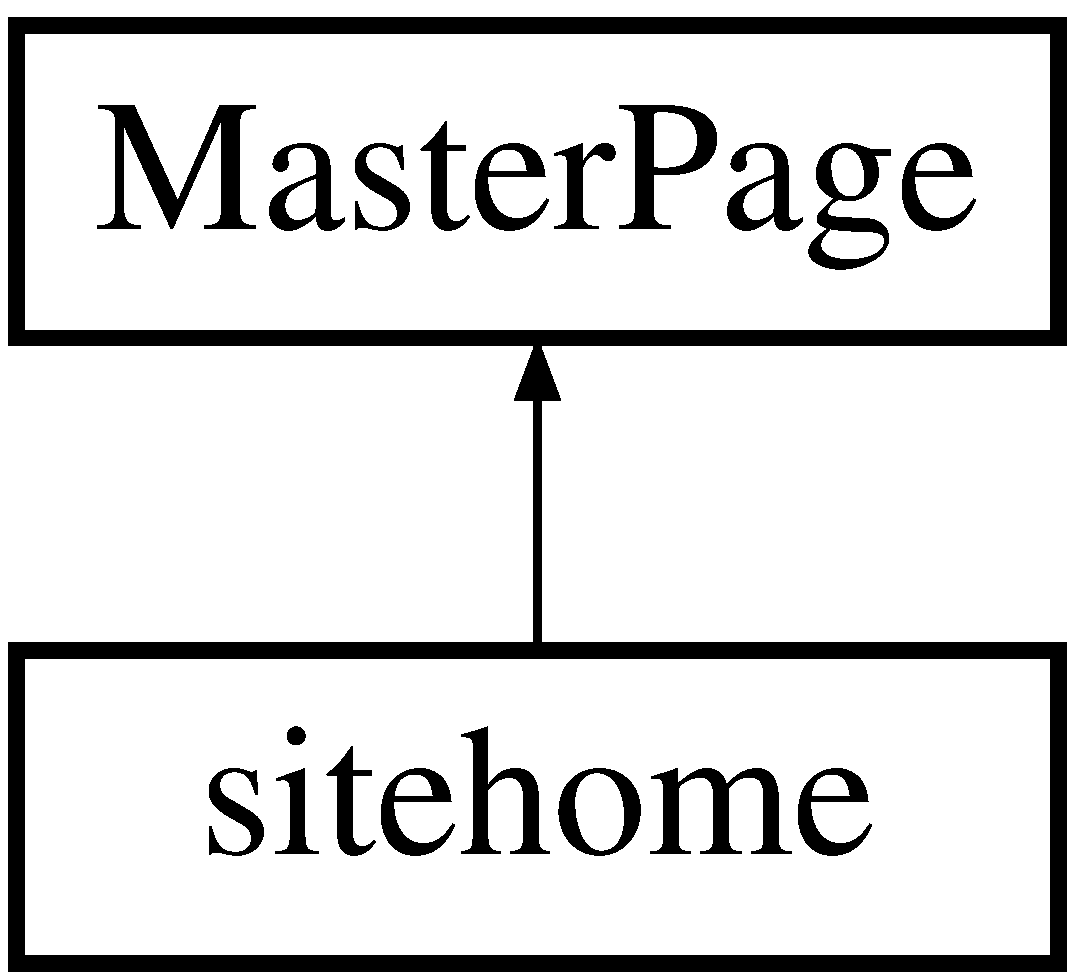
\includegraphics[height=2.000000cm]{classsitehome}
\end{center}
\end{figure}
\subsection*{Protected Member Functions}
\begin{DoxyCompactItemize}
\item 
\hypertarget{classsitehome_a3e5d32e94374bb2d2f8fd9ab72e12f39}{void {\bfseries Page\-\_\-\-Load} (object sender, Event\-Args e)}\label{classsitehome_a3e5d32e94374bb2d2f8fd9ab72e12f39}

\end{DoxyCompactItemize}


\subsection{Detailed Description}


Definition at line 8 of file sitehome.\-master.\-cs.



The documentation for this class was generated from the following file\-:\begin{DoxyCompactItemize}
\item 
E\-:/\-Mint/\-Home care/\-Smart\-Home\-Care/sitehome.\-master.\-cs\end{DoxyCompactItemize}

\hypertarget{classsiteuser}{\section{siteuser Class Reference}
\label{classsiteuser}\index{siteuser@{siteuser}}
}
Inheritance diagram for siteuser\-:\begin{figure}[H]
\begin{center}
\leavevmode
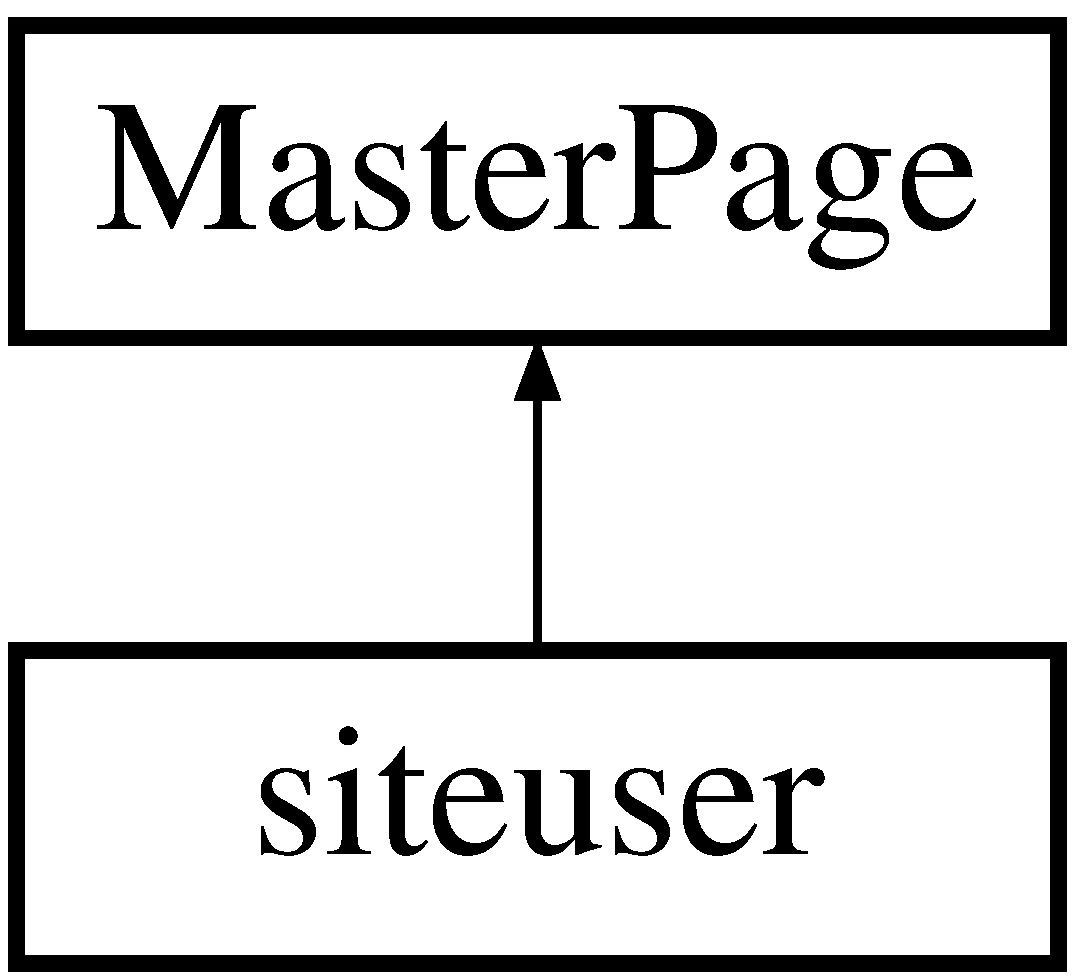
\includegraphics[height=2.000000cm]{classsiteuser}
\end{center}
\end{figure}
\subsection*{Public Attributes}
\begin{DoxyCompactItemize}
\item 
\hypertarget{classsiteuser_ab3fb80df15d4fea5c40fdee3b4b9e29a}{Tree\-View {\bfseries treeview}}\label{classsiteuser_ab3fb80df15d4fea5c40fdee3b4b9e29a}

\item 
\hypertarget{classsiteuser_a709e4be4e46130039ddc62734b99fc4c}{const int {\bfseries H\-O\-M\-E} = 0}\label{classsiteuser_a709e4be4e46130039ddc62734b99fc4c}

\item 
\hypertarget{classsiteuser_aaa470c10c3a3606b2fbab0b35103b1a5}{const int {\bfseries M\-Y\-P\-R\-O\-F\-I\-L\-E} = 1}\label{classsiteuser_aaa470c10c3a3606b2fbab0b35103b1a5}

\item 
\hypertarget{classsiteuser_a6c3ca1991850e99b719bfc5cafb73eac}{const int {\bfseries R\-E\-P\-O\-R\-T\-S} = 2}\label{classsiteuser_a6c3ca1991850e99b719bfc5cafb73eac}

\item 
\hypertarget{classsiteuser_a688cab41c9731750e4459b09f1fb7f4d}{const int {\bfseries M\-E\-S\-S\-A\-G\-E\-C\-E\-N\-T\-E\-R} = 3}\label{classsiteuser_a688cab41c9731750e4459b09f1fb7f4d}

\item 
\hypertarget{classsiteuser_a360df660979d3517879fe888b278286b}{const int {\bfseries M\-Y\-A\-C\-C\-O\-U\-N\-T} = 4}\label{classsiteuser_a360df660979d3517879fe888b278286b}

\item 
\hypertarget{classsiteuser_af8f3810eaee3c34353a6dbfaec962eb1}{const int {\bfseries U\-S\-E\-R\-I\-N\-F\-O\-R\-M\-A\-T\-I\-O\-N} = 0}\label{classsiteuser_af8f3810eaee3c34353a6dbfaec962eb1}

\item 
\hypertarget{classsiteuser_a3e6a1b9e59e65670404d950ca2041bb8}{const int {\bfseries C\-H\-A\-N\-G\-E\-P\-A\-S\-S\-W\-O\-R\-D} = 1}\label{classsiteuser_a3e6a1b9e59e65670404d950ca2041bb8}

\item 
\hypertarget{classsiteuser_a6ec77fa64dea03e82e2c0daeecbb432c}{const int {\bfseries A\-U\-T\-H\-O\-R\-I\-Z\-E\-D\-U\-S\-E\-R\-S} = 2}\label{classsiteuser_a6ec77fa64dea03e82e2c0daeecbb432c}

\item 
\hypertarget{classsiteuser_a935530c1ab32da1c025bc6d8ded0f116}{const int {\bfseries T\-R\-A\-C\-K\-M\-Y\-H\-E\-A\-L\-T\-H} = 0}\label{classsiteuser_a935530c1ab32da1c025bc6d8ded0f116}

\item 
\hypertarget{classsiteuser_ad0667582d13275c11e7b38234844a354}{const int {\bfseries T\-R\-A\-C\-K\-O\-T\-H\-E\-R\-S} = 1}\label{classsiteuser_ad0667582d13275c11e7b38234844a354}

\item 
\hypertarget{classsiteuser_a8f42529a801c3bc9c21887a227c90e9d}{const int {\bfseries C\-O\-M\-P\-O\-S\-E} = 0}\label{classsiteuser_a8f42529a801c3bc9c21887a227c90e9d}

\item 
\hypertarget{classsiteuser_a154491429ee566d5f910c65818109423}{const int {\bfseries I\-N\-B\-O\-X} = 1}\label{classsiteuser_a154491429ee566d5f910c65818109423}

\item 
\hypertarget{classsiteuser_ad477a77bb8418970f595596b3ae37c2c}{const int {\bfseries S\-E\-N\-T\-M\-E\-S\-S\-A\-G\-E\-S} = 2}\label{classsiteuser_ad477a77bb8418970f595596b3ae37c2c}

\item 
\hypertarget{classsiteuser_ab129b4c09b8cca0b8c9b28cb07748caf}{const int {\bfseries A\-L\-A\-R\-M\-M\-E\-S\-S\-A\-G\-E\-S} = 3}\label{classsiteuser_ab129b4c09b8cca0b8c9b28cb07748caf}

\item 
\hypertarget{classsiteuser_ae8231329416b314d69ad9918e52595f9}{const int {\bfseries T\-R\-A\-S\-H} = 4}\label{classsiteuser_ae8231329416b314d69ad9918e52595f9}

\item 
\hypertarget{classsiteuser_a9784e31d50b21e184774c8ca5aa09c2d}{const int {\bfseries B\-I\-L\-L\-I\-N\-G\-A\-C\-C\-O\-U\-N\-T\-S\-U\-M\-M\-A\-R} = 0}\label{classsiteuser_a9784e31d50b21e184774c8ca5aa09c2d}

\item 
\hypertarget{classsiteuser_a7ddfc011da7772e39d038eefcd62e85c}{const int {\bfseries C\-O\-V\-E\-R\-R\-A\-G\-E\-D\-E\-T\-A\-I\-L\-S} = 1}\label{classsiteuser_a7ddfc011da7772e39d038eefcd62e85c}

\end{DoxyCompactItemize}
\subsection*{Protected Member Functions}
\begin{DoxyCompactItemize}
\item 
\hypertarget{classsiteuser_abb11093e15d594ac1178269d753b2d24}{void {\bfseries Page\-\_\-\-Init} (object sender, Event\-Args e)}\label{classsiteuser_abb11093e15d594ac1178269d753b2d24}

\item 
\hypertarget{classsiteuser_aa41ca54631613bf74dad2583ff3ef205}{void {\bfseries Page\-\_\-\-Load} (object sender, Event\-Args e)}\label{classsiteuser_aa41ca54631613bf74dad2583ff3ef205}

\end{DoxyCompactItemize}


\subsection{Detailed Description}


Definition at line 9 of file siteuser.\-master.\-cs.



The documentation for this class was generated from the following file\-:\begin{DoxyCompactItemize}
\item 
E\-:/\-Mint/\-Home care/\-Smart\-Home\-Care/siteuser.\-master.\-cs\end{DoxyCompactItemize}

\hypertarget{class_stee_chart}{\section{Stee\-Chart Class Reference}
\label{class_stee_chart}\index{Stee\-Chart@{Stee\-Chart}}
}
Inheritance diagram for Stee\-Chart\-:\begin{figure}[H]
\begin{center}
\leavevmode
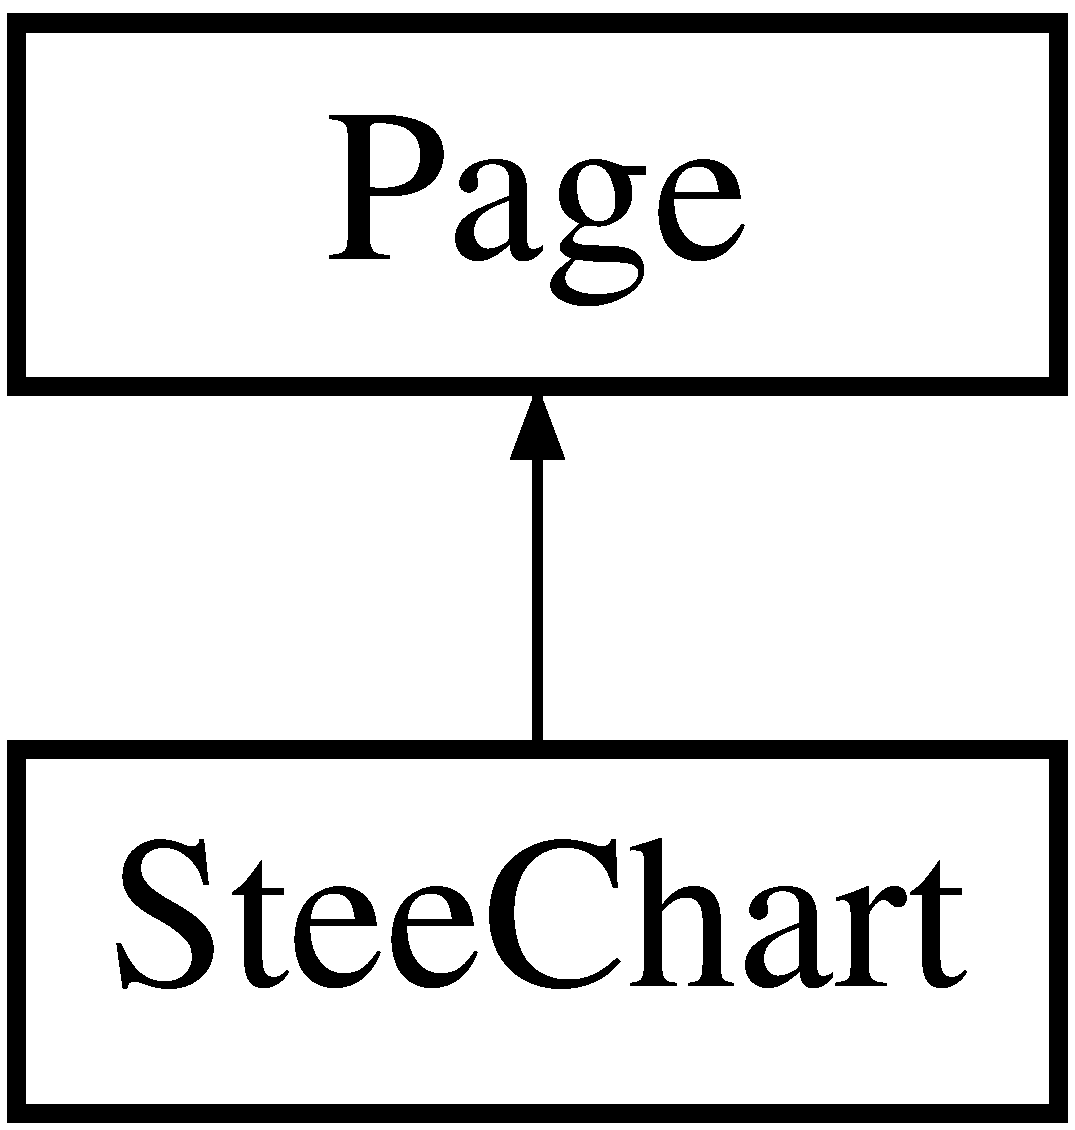
\includegraphics[height=2.000000cm]{class_stee_chart}
\end{center}
\end{figure}
\subsection*{Protected Member Functions}
\begin{DoxyCompactItemize}
\item 
\hypertarget{class_stee_chart_a16d02558edab938b7526b950e15f38f5}{void {\bfseries Page\-\_\-\-Load} (object sender, Event\-Args e)}\label{class_stee_chart_a16d02558edab938b7526b950e15f38f5}

\item 
\hypertarget{class_stee_chart_ae3ae7db4a3dc5cd39de2175cf29c9e47}{void {\bfseries Drop\-Down\-List1\-\_\-\-Selected\-Index\-Changed} (object sender, Event\-Args e)}\label{class_stee_chart_ae3ae7db4a3dc5cd39de2175cf29c9e47}

\item 
\hypertarget{class_stee_chart_a911c61c6fc34efd1e6951e3854864475}{void {\bfseries Web\-Chart1\-\_\-\-Get\-Axis\-Label} (object sender, Steema.\-Tee\-Chart.\-Get\-Axis\-Label\-Event\-Args e)}\label{class_stee_chart_a911c61c6fc34efd1e6951e3854864475}

\item 
\hypertarget{class_stee_chart_a1452884b58ca9507dcc55c55fc3dda22}{void {\bfseries Web\-Chart1\-\_\-\-Click\-Axis} (object sender, Image\-Click\-Event\-Args e)}\label{class_stee_chart_a1452884b58ca9507dcc55c55fc3dda22}

\item 
\hypertarget{class_stee_chart_aa01fd5552c7a4c931cb7cdf8332e0941}{void {\bfseries Web\-Chart1\-\_\-\-After\-Draw} (object sender, Steema.\-Tee\-Chart.\-Drawing.\-Graphics3\-D g)}\label{class_stee_chart_aa01fd5552c7a4c931cb7cdf8332e0941}

\item 
\hypertarget{class_stee_chart_a6e44f9a787a631f07a41f25bbe7acb05}{void {\bfseries Web\-Chart1\-\_\-\-Click\-Series} (object sender, Series s, int value\-Index, Event\-Args e)}\label{class_stee_chart_a6e44f9a787a631f07a41f25bbe7acb05}

\item 
\hypertarget{class_stee_chart_a9bedfef7dfb7a42db4b5f9616ec33305}{void {\bfseries Button1\-\_\-\-Click} (object sender, Event\-Args e)}\label{class_stee_chart_a9bedfef7dfb7a42db4b5f9616ec33305}

\end{DoxyCompactItemize}


\subsection{Detailed Description}


Definition at line 15 of file Stee\-Chart.\-aspx.\-cs.



The documentation for this class was generated from the following file\-:\begin{DoxyCompactItemize}
\item 
E\-:/\-Mint/\-Home care/\-Smart\-Home\-Care/Stee\-Chart.\-aspx.\-cs\end{DoxyCompactItemize}

\hypertarget{class_steechart2}{\section{Steechart2 Class Reference}
\label{class_steechart2}\index{Steechart2@{Steechart2}}
}
Inheritance diagram for Steechart2\-:\begin{figure}[H]
\begin{center}
\leavevmode
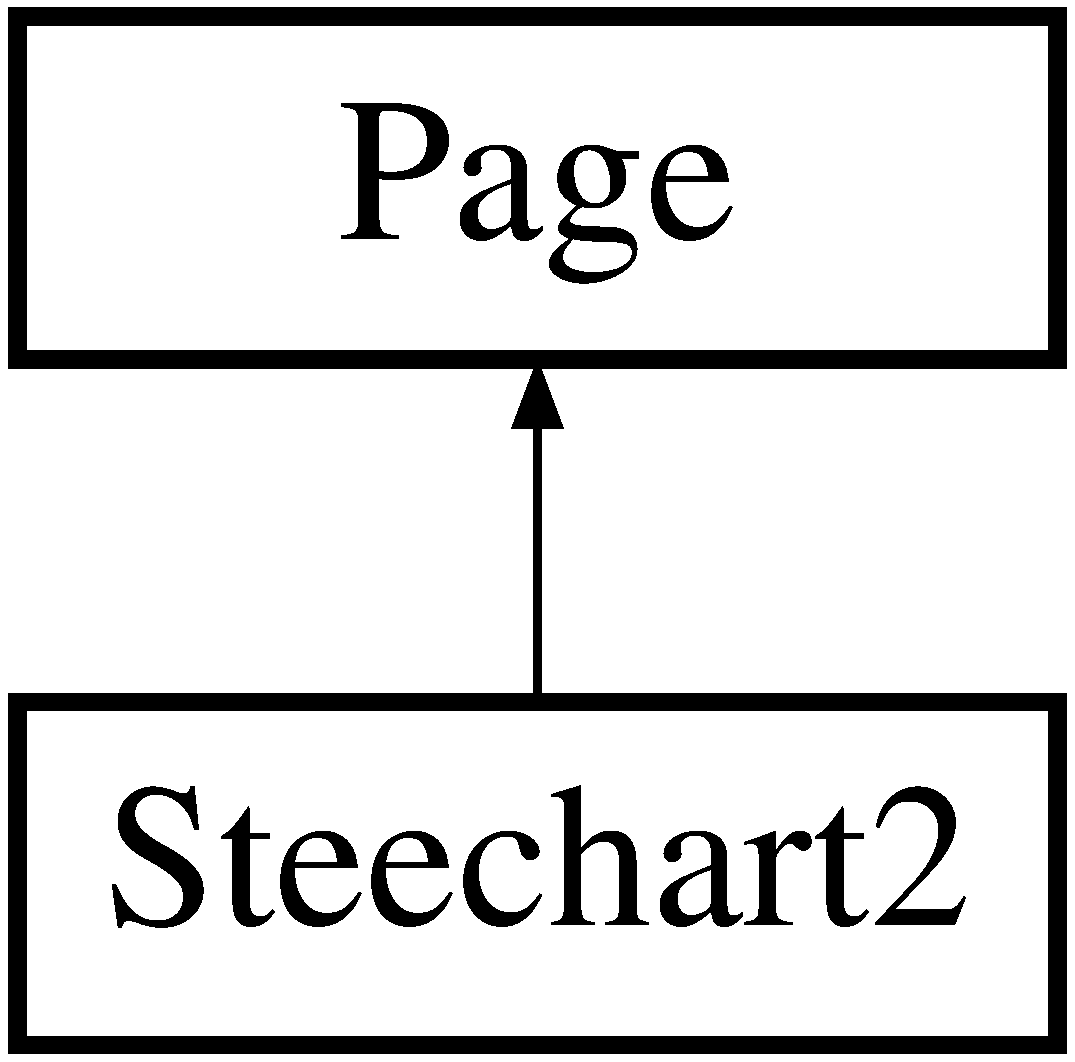
\includegraphics[height=2.000000cm]{class_steechart2}
\end{center}
\end{figure}
\subsection*{Protected Member Functions}
\begin{DoxyCompactItemize}
\item 
\hypertarget{class_steechart2_afc5fbe8a9b611e83c258c31cff4f699d}{void {\bfseries Page\-\_\-\-Load} (object sender, Event\-Args e)}\label{class_steechart2_afc5fbe8a9b611e83c258c31cff4f699d}

\end{DoxyCompactItemize}


\subsection{Detailed Description}


Definition at line 16 of file Steechart2.\-aspx.\-cs.



The documentation for this class was generated from the following file\-:\begin{DoxyCompactItemize}
\item 
E\-:/\-Mint/\-Home care/\-Smart\-Home\-Care/Steechart2.\-aspx.\-cs\end{DoxyCompactItemize}

\hypertarget{classtermsandconditions}{\section{termsandconditions Class Reference}
\label{classtermsandconditions}\index{termsandconditions@{termsandconditions}}
}
Inheritance diagram for termsandconditions\-:\begin{figure}[H]
\begin{center}
\leavevmode
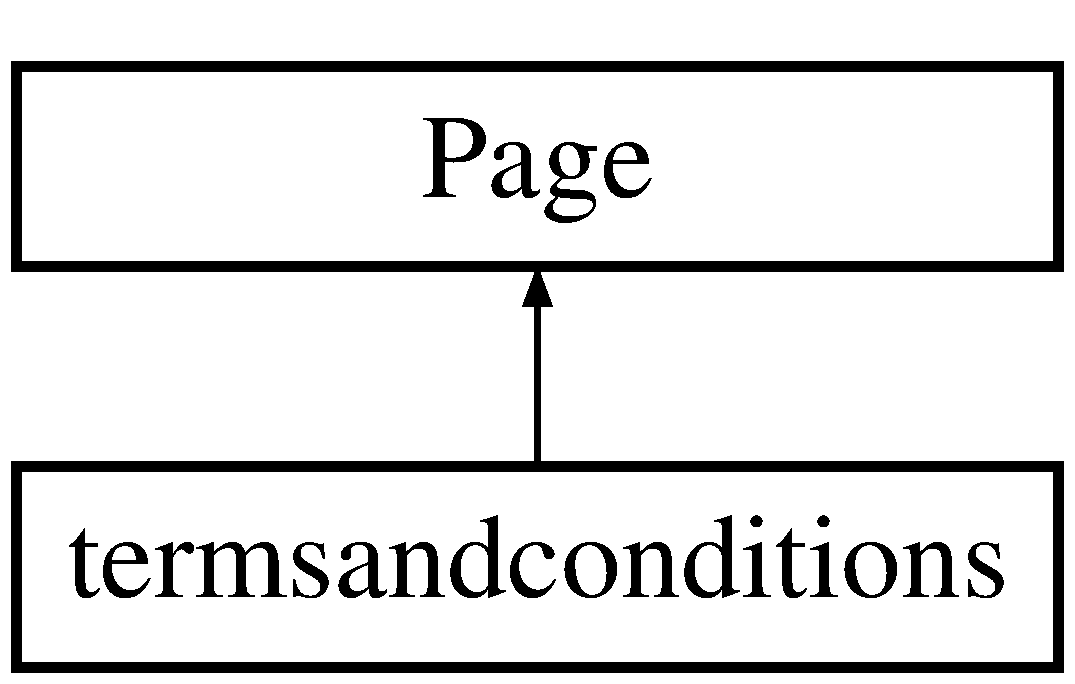
\includegraphics[height=2.000000cm]{classtermsandconditions}
\end{center}
\end{figure}
\subsection*{Protected Member Functions}
\begin{DoxyCompactItemize}
\item 
\hypertarget{classtermsandconditions_a72071d075dca165af6884d9314f29a79}{void {\bfseries Page\-\_\-\-Load} (object sender, Event\-Args e)}\label{classtermsandconditions_a72071d075dca165af6884d9314f29a79}

\end{DoxyCompactItemize}


\subsection{Detailed Description}


Definition at line 8 of file termsandconditions.\-aspx.\-cs.



The documentation for this class was generated from the following file\-:\begin{DoxyCompactItemize}
\item 
E\-:/\-Mint/\-Home care/\-Smart\-Home\-Care/termsandconditions.\-aspx.\-cs\end{DoxyCompactItemize}

\hypertarget{classtest}{\section{test Class Reference}
\label{classtest}\index{test@{test}}
}
Inheritance diagram for test\-:\begin{figure}[H]
\begin{center}
\leavevmode
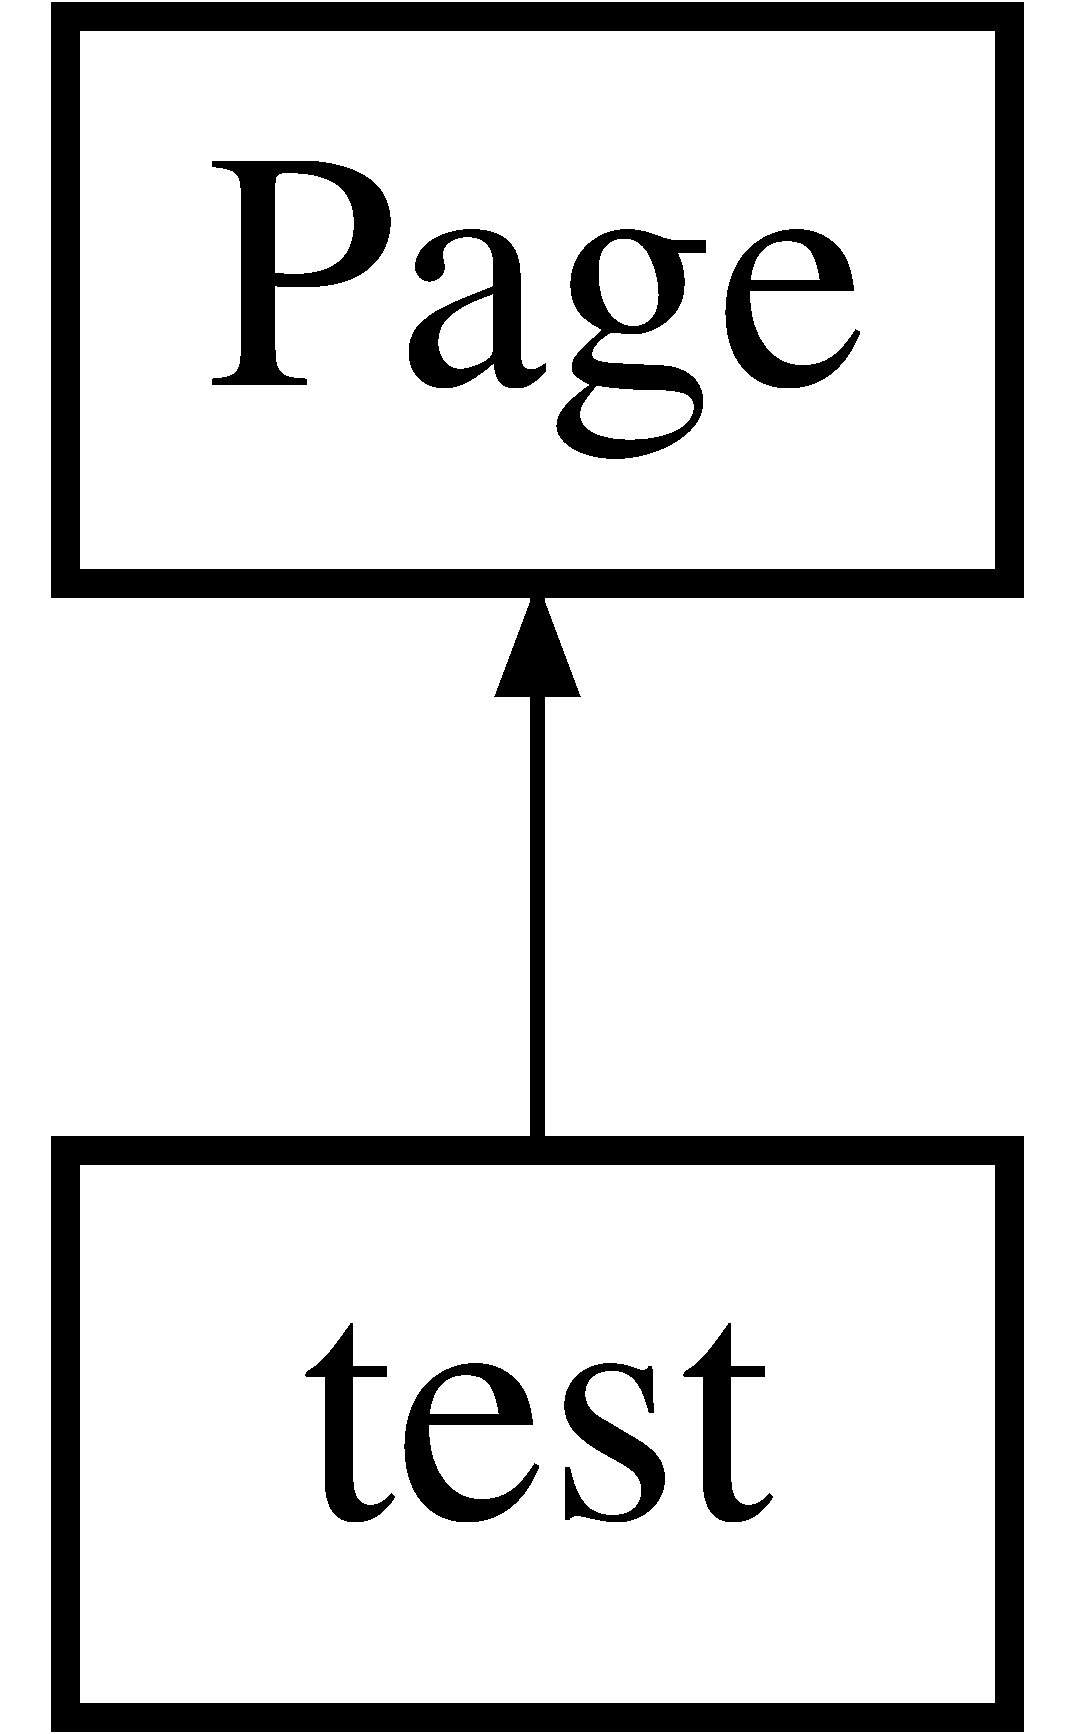
\includegraphics[height=2.000000cm]{classtest}
\end{center}
\end{figure}
\subsection*{Static Public Attributes}
\begin{DoxyCompactItemize}
\item 
\hypertarget{classtest_aba0f828b97e0e7b1bb62fad562eebb2c}{static int {\bfseries i} =1}\label{classtest_aba0f828b97e0e7b1bb62fad562eebb2c}

\end{DoxyCompactItemize}
\subsection*{Protected Member Functions}
\begin{DoxyCompactItemize}
\item 
\hypertarget{classtest_abf4d31a76a10eccc3764d0f6e7459490}{void {\bfseries Page\-\_\-\-Load} (object sender, Event\-Args e)}\label{classtest_abf4d31a76a10eccc3764d0f6e7459490}

\item 
\hypertarget{classtest_a50c23d16f9406ccb3d03f2fe26cf6727}{void {\bfseries btn\-Next\-\_\-\-Click} (object sender, Event\-Args e)}\label{classtest_a50c23d16f9406ccb3d03f2fe26cf6727}

\item 
\hypertarget{classtest_a31cfe2c19bc0fa1a2a3dc80ac8185331}{void {\bfseries btn\-\_\-back\-\_\-\-Click} (object sender, Event\-Args e)}\label{classtest_a31cfe2c19bc0fa1a2a3dc80ac8185331}

\end{DoxyCompactItemize}


\subsection{Detailed Description}


Definition at line 8 of file test.\-aspx.\-cs.



The documentation for this class was generated from the following file\-:\begin{DoxyCompactItemize}
\item 
E\-:/\-Mint/\-Home care/\-Smart\-Home\-Care/test.\-aspx.\-cs\end{DoxyCompactItemize}

\hypertarget{class_to_s_q_l}{\section{To\-S\-Q\-L Class Reference}
\label{class_to_s_q_l}\index{To\-S\-Q\-L@{To\-S\-Q\-L}}
}


convert data  


\subsection*{Static Public Member Functions}
\begin{DoxyCompactItemize}
\item 
static string \hyperlink{class_to_s_q_l_a924feba5689640b9260c7ff4d4da2df3}{Empty\-Null} (object Obj)
\item 
static int \hyperlink{class_to_s_q_l_a84a04e64766978cecdba0eaeb6252f80}{S\-Q\-L\-To\-Int} (object Obj)
\item 
static int \hyperlink{class_to_s_q_l_a861e05fe50c8425d6a3f964fc2c45299}{S\-Q\-L\-To\-Int\-Null} (object Obj)
\item 
static decimal \hyperlink{class_to_s_q_l_ad872e7782e533bfea0c3fcc64214b4e0}{S\-Q\-L\-To\-Decimal} (object Obj)
\item 
static decimal \hyperlink{class_to_s_q_l_afdaef8db307e9ae4a543a9dcc6e700a0}{S\-Q\-L\-To\-Decimal\-Null} (object Obj)
\item 
static double \hyperlink{class_to_s_q_l_a1bd370378625d1fc19ee47b35d29b2d3}{S\-Q\-L\-To\-Double} (object Obj)
\item 
static bool \hyperlink{class_to_s_q_l_abea8cc7efc15e6ed898c47300709d56b}{S\-Q\-L\-To\-Bool} (object Obj)
\item 
static Date\-Time \hyperlink{class_to_s_q_l_a5c0dc88c118676c5f4c581b4434dc45a}{S\-Q\-L\-To\-Date\-Time} (object Obj)
\item 
static bool \hyperlink{class_to_s_q_l_a0f8d0c3fed178000d9f29a1ed046caa4}{Is\-Numberic} (object Obj)
\item 
static bool \hyperlink{class_to_s_q_l_a5ea5080d0c22668757d8289f8426e219}{Is\-Date} (object Obj)
\item 
static string \hyperlink{class_to_s_q_l_a125bc678eb4a1342a78ce05baa97c218}{S\-Q\-L\-String} (object Obj)
\item 
static string \hyperlink{class_to_s_q_l_ad5faed3305f877b3dc46360cadd93add}{S\-Q\-L\-U\-String} (object Obj)
\item 
static string \hyperlink{class_to_s_q_l_aded0150550c536d79ecbb7da1fa71022}{S\-Q\-L\-Like\-String} (object Obj)
\item 
static string \hyperlink{class_to_s_q_l_ad1b42e655d19e5ab7217c03a1c66779e}{S\-Q\-L\-Numeric} (object Obj)
\item 
static string \hyperlink{class_to_s_q_l_a49c612e4bef2c6a74b54d9d1486e9b39}{S\-Q\-L\-Bit} (object Obj)
\item 
static string \hyperlink{class_to_s_q_l_a35bbf54ca70c4d825eb74233c0ba2c22}{S\-Q\-L\-Bit\-Null} (object Obj)
\item 
static string \hyperlink{class_to_s_q_l_aaa27de46f75cdc8ef0176ec338975d51}{S\-Q\-L\-Date} (Date\-Time?Obj)
\item 
static Date\-Time \hyperlink{class_to_s_q_l_a070eca2f694ccc73c60617bdaa9c7d33}{S\-Q\-L\-To\-Date\-Time24\-H} (string Obj)
\item 
static string \hyperlink{class_to_s_q_l_a61bb97099c6a430730fe4c29dd7c8b68}{S\-Q\-L\-Date\-Non\-Hour} (Date\-Time Obj)
\end{DoxyCompactItemize}


\subsection{Detailed Description}
convert data 

Definition at line 9 of file To\-S\-Q\-L.\-cs.



\subsection{Member Function Documentation}
\hypertarget{class_to_s_q_l_a924feba5689640b9260c7ff4d4da2df3}{\index{To\-S\-Q\-L@{To\-S\-Q\-L}!Empty\-Null@{Empty\-Null}}
\index{Empty\-Null@{Empty\-Null}!ToSQL@{To\-S\-Q\-L}}
\subsubsection[{Empty\-Null}]{\setlength{\rightskip}{0pt plus 5cm}static string To\-S\-Q\-L.\-Empty\-Null (
\begin{DoxyParamCaption}
\item[{object}]{Obj}
\end{DoxyParamCaption}
)\hspace{0.3cm}{\ttfamily [static]}}}\label{class_to_s_q_l_a924feba5689640b9260c7ff4d4da2df3}
convert object to string \begin{DoxySeeAlso}{See Also}
\hyperlink{class_to_s_q_l_a924feba5689640b9260c7ff4d4da2df3}{Empty\-Null()} 
\end{DoxySeeAlso}


Definition at line 15 of file To\-S\-Q\-L.\-cs.

\hypertarget{class_to_s_q_l_a5ea5080d0c22668757d8289f8426e219}{\index{To\-S\-Q\-L@{To\-S\-Q\-L}!Is\-Date@{Is\-Date}}
\index{Is\-Date@{Is\-Date}!ToSQL@{To\-S\-Q\-L}}
\subsubsection[{Is\-Date}]{\setlength{\rightskip}{0pt plus 5cm}static bool To\-S\-Q\-L.\-Is\-Date (
\begin{DoxyParamCaption}
\item[{object}]{Obj}
\end{DoxyParamCaption}
)\hspace{0.3cm}{\ttfamily [static]}}}\label{class_to_s_q_l_a5ea5080d0c22668757d8289f8426e219}
check object is date \begin{DoxySeeAlso}{See Also}
\hyperlink{class_to_s_q_l_a5ea5080d0c22668757d8289f8426e219}{Is\-Date()} 
\end{DoxySeeAlso}


Definition at line 143 of file To\-S\-Q\-L.\-cs.

\hypertarget{class_to_s_q_l_a0f8d0c3fed178000d9f29a1ed046caa4}{\index{To\-S\-Q\-L@{To\-S\-Q\-L}!Is\-Numberic@{Is\-Numberic}}
\index{Is\-Numberic@{Is\-Numberic}!ToSQL@{To\-S\-Q\-L}}
\subsubsection[{Is\-Numberic}]{\setlength{\rightskip}{0pt plus 5cm}static bool To\-S\-Q\-L.\-Is\-Numberic (
\begin{DoxyParamCaption}
\item[{object}]{Obj}
\end{DoxyParamCaption}
)\hspace{0.3cm}{\ttfamily [static]}}}\label{class_to_s_q_l_a0f8d0c3fed178000d9f29a1ed046caa4}
check object is numberic \begin{DoxySeeAlso}{See Also}
\hyperlink{class_to_s_q_l_a0f8d0c3fed178000d9f29a1ed046caa4}{Is\-Numberic()} 
\end{DoxySeeAlso}


Definition at line 127 of file To\-S\-Q\-L.\-cs.

\hypertarget{class_to_s_q_l_a49c612e4bef2c6a74b54d9d1486e9b39}{\index{To\-S\-Q\-L@{To\-S\-Q\-L}!S\-Q\-L\-Bit@{S\-Q\-L\-Bit}}
\index{S\-Q\-L\-Bit@{S\-Q\-L\-Bit}!ToSQL@{To\-S\-Q\-L}}
\subsubsection[{S\-Q\-L\-Bit}]{\setlength{\rightskip}{0pt plus 5cm}static string To\-S\-Q\-L.\-S\-Q\-L\-Bit (
\begin{DoxyParamCaption}
\item[{object}]{Obj}
\end{DoxyParamCaption}
)\hspace{0.3cm}{\ttfamily [static]}}}\label{class_to_s_q_l_a49c612e4bef2c6a74b54d9d1486e9b39}
convert object to string \begin{DoxySeeAlso}{See Also}
\hyperlink{class_to_s_q_l_a49c612e4bef2c6a74b54d9d1486e9b39}{S\-Q\-L\-Bit()} 
\end{DoxySeeAlso}


Definition at line 201 of file To\-S\-Q\-L.\-cs.

\hypertarget{class_to_s_q_l_a35bbf54ca70c4d825eb74233c0ba2c22}{\index{To\-S\-Q\-L@{To\-S\-Q\-L}!S\-Q\-L\-Bit\-Null@{S\-Q\-L\-Bit\-Null}}
\index{S\-Q\-L\-Bit\-Null@{S\-Q\-L\-Bit\-Null}!ToSQL@{To\-S\-Q\-L}}
\subsubsection[{S\-Q\-L\-Bit\-Null}]{\setlength{\rightskip}{0pt plus 5cm}static string To\-S\-Q\-L.\-S\-Q\-L\-Bit\-Null (
\begin{DoxyParamCaption}
\item[{object}]{Obj}
\end{DoxyParamCaption}
)\hspace{0.3cm}{\ttfamily [static]}}}\label{class_to_s_q_l_a35bbf54ca70c4d825eb74233c0ba2c22}
convert object to string \begin{DoxySeeAlso}{See Also}
\hyperlink{class_to_s_q_l_a35bbf54ca70c4d825eb74233c0ba2c22}{S\-Q\-L\-Bit\-Null()} 
\end{DoxySeeAlso}


Definition at line 211 of file To\-S\-Q\-L.\-cs.

\hypertarget{class_to_s_q_l_aaa27de46f75cdc8ef0176ec338975d51}{\index{To\-S\-Q\-L@{To\-S\-Q\-L}!S\-Q\-L\-Date@{S\-Q\-L\-Date}}
\index{S\-Q\-L\-Date@{S\-Q\-L\-Date}!ToSQL@{To\-S\-Q\-L}}
\subsubsection[{S\-Q\-L\-Date}]{\setlength{\rightskip}{0pt plus 5cm}static string To\-S\-Q\-L.\-S\-Q\-L\-Date (
\begin{DoxyParamCaption}
\item[{Date\-Time?}]{Obj}
\end{DoxyParamCaption}
)\hspace{0.3cm}{\ttfamily [static]}}}\label{class_to_s_q_l_aaa27de46f75cdc8ef0176ec338975d51}
convert date to string \begin{DoxySeeAlso}{See Also}
\hyperlink{class_to_s_q_l_aaa27de46f75cdc8ef0176ec338975d51}{S\-Q\-L\-Date()} 
\end{DoxySeeAlso}


Definition at line 226 of file To\-S\-Q\-L.\-cs.

\hypertarget{class_to_s_q_l_a61bb97099c6a430730fe4c29dd7c8b68}{\index{To\-S\-Q\-L@{To\-S\-Q\-L}!S\-Q\-L\-Date\-Non\-Hour@{S\-Q\-L\-Date\-Non\-Hour}}
\index{S\-Q\-L\-Date\-Non\-Hour@{S\-Q\-L\-Date\-Non\-Hour}!ToSQL@{To\-S\-Q\-L}}
\subsubsection[{S\-Q\-L\-Date\-Non\-Hour}]{\setlength{\rightskip}{0pt plus 5cm}static string To\-S\-Q\-L.\-S\-Q\-L\-Date\-Non\-Hour (
\begin{DoxyParamCaption}
\item[{Date\-Time}]{Obj}
\end{DoxyParamCaption}
)\hspace{0.3cm}{\ttfamily [static]}}}\label{class_to_s_q_l_a61bb97099c6a430730fe4c29dd7c8b68}
convert date to string \begin{DoxySeeAlso}{See Also}
\hyperlink{class_to_s_q_l_a61bb97099c6a430730fe4c29dd7c8b68}{S\-Q\-L\-Date\-Non\-Hour()} 
\end{DoxySeeAlso}


Definition at line 260 of file To\-S\-Q\-L.\-cs.

\hypertarget{class_to_s_q_l_aded0150550c536d79ecbb7da1fa71022}{\index{To\-S\-Q\-L@{To\-S\-Q\-L}!S\-Q\-L\-Like\-String@{S\-Q\-L\-Like\-String}}
\index{S\-Q\-L\-Like\-String@{S\-Q\-L\-Like\-String}!ToSQL@{To\-S\-Q\-L}}
\subsubsection[{S\-Q\-L\-Like\-String}]{\setlength{\rightskip}{0pt plus 5cm}static string To\-S\-Q\-L.\-S\-Q\-L\-Like\-String (
\begin{DoxyParamCaption}
\item[{object}]{Obj}
\end{DoxyParamCaption}
)\hspace{0.3cm}{\ttfamily [static]}}}\label{class_to_s_q_l_aded0150550c536d79ecbb7da1fa71022}
convert object to string \begin{DoxySeeAlso}{See Also}
\hyperlink{class_to_s_q_l_aded0150550c536d79ecbb7da1fa71022}{S\-Q\-L\-Like\-String()} 
\end{DoxySeeAlso}


Definition at line 179 of file To\-S\-Q\-L.\-cs.

\hypertarget{class_to_s_q_l_ad1b42e655d19e5ab7217c03a1c66779e}{\index{To\-S\-Q\-L@{To\-S\-Q\-L}!S\-Q\-L\-Numeric@{S\-Q\-L\-Numeric}}
\index{S\-Q\-L\-Numeric@{S\-Q\-L\-Numeric}!ToSQL@{To\-S\-Q\-L}}
\subsubsection[{S\-Q\-L\-Numeric}]{\setlength{\rightskip}{0pt plus 5cm}static string To\-S\-Q\-L.\-S\-Q\-L\-Numeric (
\begin{DoxyParamCaption}
\item[{object}]{Obj}
\end{DoxyParamCaption}
)\hspace{0.3cm}{\ttfamily [static]}}}\label{class_to_s_q_l_ad1b42e655d19e5ab7217c03a1c66779e}
convert object to string \begin{DoxySeeAlso}{See Also}
\hyperlink{class_to_s_q_l_ad1b42e655d19e5ab7217c03a1c66779e}{S\-Q\-L\-Numeric()} 
\end{DoxySeeAlso}


Definition at line 189 of file To\-S\-Q\-L.\-cs.

\hypertarget{class_to_s_q_l_a125bc678eb4a1342a78ce05baa97c218}{\index{To\-S\-Q\-L@{To\-S\-Q\-L}!S\-Q\-L\-String@{S\-Q\-L\-String}}
\index{S\-Q\-L\-String@{S\-Q\-L\-String}!ToSQL@{To\-S\-Q\-L}}
\subsubsection[{S\-Q\-L\-String}]{\setlength{\rightskip}{0pt plus 5cm}static string To\-S\-Q\-L.\-S\-Q\-L\-String (
\begin{DoxyParamCaption}
\item[{object}]{Obj}
\end{DoxyParamCaption}
)\hspace{0.3cm}{\ttfamily [static]}}}\label{class_to_s_q_l_a125bc678eb4a1342a78ce05baa97c218}
convert object to string \begin{DoxySeeAlso}{See Also}
\hyperlink{class_to_s_q_l_a125bc678eb4a1342a78ce05baa97c218}{S\-Q\-L\-String()} 
\end{DoxySeeAlso}


Definition at line 159 of file To\-S\-Q\-L.\-cs.

\hypertarget{class_to_s_q_l_abea8cc7efc15e6ed898c47300709d56b}{\index{To\-S\-Q\-L@{To\-S\-Q\-L}!S\-Q\-L\-To\-Bool@{S\-Q\-L\-To\-Bool}}
\index{S\-Q\-L\-To\-Bool@{S\-Q\-L\-To\-Bool}!ToSQL@{To\-S\-Q\-L}}
\subsubsection[{S\-Q\-L\-To\-Bool}]{\setlength{\rightskip}{0pt plus 5cm}static bool To\-S\-Q\-L.\-S\-Q\-L\-To\-Bool (
\begin{DoxyParamCaption}
\item[{object}]{Obj}
\end{DoxyParamCaption}
)\hspace{0.3cm}{\ttfamily [static]}}}\label{class_to_s_q_l_abea8cc7efc15e6ed898c47300709d56b}
convert object to bool \begin{DoxySeeAlso}{See Also}
\hyperlink{class_to_s_q_l_abea8cc7efc15e6ed898c47300709d56b}{S\-Q\-L\-To\-Bool()} 
\end{DoxySeeAlso}


Definition at line 96 of file To\-S\-Q\-L.\-cs.

\hypertarget{class_to_s_q_l_a5c0dc88c118676c5f4c581b4434dc45a}{\index{To\-S\-Q\-L@{To\-S\-Q\-L}!S\-Q\-L\-To\-Date\-Time@{S\-Q\-L\-To\-Date\-Time}}
\index{S\-Q\-L\-To\-Date\-Time@{S\-Q\-L\-To\-Date\-Time}!ToSQL@{To\-S\-Q\-L}}
\subsubsection[{S\-Q\-L\-To\-Date\-Time}]{\setlength{\rightskip}{0pt plus 5cm}static Date\-Time To\-S\-Q\-L.\-S\-Q\-L\-To\-Date\-Time (
\begin{DoxyParamCaption}
\item[{object}]{Obj}
\end{DoxyParamCaption}
)\hspace{0.3cm}{\ttfamily [static]}}}\label{class_to_s_q_l_a5c0dc88c118676c5f4c581b4434dc45a}
convert object to date \begin{DoxySeeAlso}{See Also}
\hyperlink{class_to_s_q_l_a5c0dc88c118676c5f4c581b4434dc45a}{S\-Q\-L\-To\-Date\-Time()} 
\end{DoxySeeAlso}


Definition at line 111 of file To\-S\-Q\-L.\-cs.

\hypertarget{class_to_s_q_l_a070eca2f694ccc73c60617bdaa9c7d33}{\index{To\-S\-Q\-L@{To\-S\-Q\-L}!S\-Q\-L\-To\-Date\-Time24\-H@{S\-Q\-L\-To\-Date\-Time24\-H}}
\index{S\-Q\-L\-To\-Date\-Time24\-H@{S\-Q\-L\-To\-Date\-Time24\-H}!ToSQL@{To\-S\-Q\-L}}
\subsubsection[{S\-Q\-L\-To\-Date\-Time24\-H}]{\setlength{\rightskip}{0pt plus 5cm}static Date\-Time To\-S\-Q\-L.\-S\-Q\-L\-To\-Date\-Time24\-H (
\begin{DoxyParamCaption}
\item[{string}]{Obj}
\end{DoxyParamCaption}
)\hspace{0.3cm}{\ttfamily [static]}}}\label{class_to_s_q_l_a070eca2f694ccc73c60617bdaa9c7d33}
convert string to date \begin{DoxySeeAlso}{See Also}
\hyperlink{class_to_s_q_l_a070eca2f694ccc73c60617bdaa9c7d33}{S\-Q\-L\-To\-Date\-Time24\-H()} 
\end{DoxySeeAlso}


Definition at line 242 of file To\-S\-Q\-L.\-cs.

\hypertarget{class_to_s_q_l_ad872e7782e533bfea0c3fcc64214b4e0}{\index{To\-S\-Q\-L@{To\-S\-Q\-L}!S\-Q\-L\-To\-Decimal@{S\-Q\-L\-To\-Decimal}}
\index{S\-Q\-L\-To\-Decimal@{S\-Q\-L\-To\-Decimal}!ToSQL@{To\-S\-Q\-L}}
\subsubsection[{S\-Q\-L\-To\-Decimal}]{\setlength{\rightskip}{0pt plus 5cm}static decimal To\-S\-Q\-L.\-S\-Q\-L\-To\-Decimal (
\begin{DoxyParamCaption}
\item[{object}]{Obj}
\end{DoxyParamCaption}
)\hspace{0.3cm}{\ttfamily [static]}}}\label{class_to_s_q_l_ad872e7782e533bfea0c3fcc64214b4e0}
convert object to decimal \begin{DoxySeeAlso}{See Also}
\hyperlink{class_to_s_q_l_ad872e7782e533bfea0c3fcc64214b4e0}{S\-Q\-L\-To\-Decimal()} 
\end{DoxySeeAlso}


Definition at line 55 of file To\-S\-Q\-L.\-cs.

\hypertarget{class_to_s_q_l_afdaef8db307e9ae4a543a9dcc6e700a0}{\index{To\-S\-Q\-L@{To\-S\-Q\-L}!S\-Q\-L\-To\-Decimal\-Null@{S\-Q\-L\-To\-Decimal\-Null}}
\index{S\-Q\-L\-To\-Decimal\-Null@{S\-Q\-L\-To\-Decimal\-Null}!ToSQL@{To\-S\-Q\-L}}
\subsubsection[{S\-Q\-L\-To\-Decimal\-Null}]{\setlength{\rightskip}{0pt plus 5cm}static decimal To\-S\-Q\-L.\-S\-Q\-L\-To\-Decimal\-Null (
\begin{DoxyParamCaption}
\item[{object}]{Obj}
\end{DoxyParamCaption}
)\hspace{0.3cm}{\ttfamily [static]}}}\label{class_to_s_q_l_afdaef8db307e9ae4a543a9dcc6e700a0}
convert object to decimal \begin{DoxySeeAlso}{See Also}
\hyperlink{class_to_s_q_l_afdaef8db307e9ae4a543a9dcc6e700a0}{S\-Q\-L\-To\-Decimal\-Null()} 
\end{DoxySeeAlso}


Definition at line 70 of file To\-S\-Q\-L.\-cs.

\hypertarget{class_to_s_q_l_a1bd370378625d1fc19ee47b35d29b2d3}{\index{To\-S\-Q\-L@{To\-S\-Q\-L}!S\-Q\-L\-To\-Double@{S\-Q\-L\-To\-Double}}
\index{S\-Q\-L\-To\-Double@{S\-Q\-L\-To\-Double}!ToSQL@{To\-S\-Q\-L}}
\subsubsection[{S\-Q\-L\-To\-Double}]{\setlength{\rightskip}{0pt plus 5cm}static double To\-S\-Q\-L.\-S\-Q\-L\-To\-Double (
\begin{DoxyParamCaption}
\item[{object}]{Obj}
\end{DoxyParamCaption}
)\hspace{0.3cm}{\ttfamily [static]}}}\label{class_to_s_q_l_a1bd370378625d1fc19ee47b35d29b2d3}
convert object to double \begin{DoxySeeAlso}{See Also}
\hyperlink{class_to_s_q_l_a1bd370378625d1fc19ee47b35d29b2d3}{S\-Q\-L\-To\-Double()} 
\end{DoxySeeAlso}


Definition at line 81 of file To\-S\-Q\-L.\-cs.

\hypertarget{class_to_s_q_l_a84a04e64766978cecdba0eaeb6252f80}{\index{To\-S\-Q\-L@{To\-S\-Q\-L}!S\-Q\-L\-To\-Int@{S\-Q\-L\-To\-Int}}
\index{S\-Q\-L\-To\-Int@{S\-Q\-L\-To\-Int}!ToSQL@{To\-S\-Q\-L}}
\subsubsection[{S\-Q\-L\-To\-Int}]{\setlength{\rightskip}{0pt plus 5cm}static int To\-S\-Q\-L.\-S\-Q\-L\-To\-Int (
\begin{DoxyParamCaption}
\item[{object}]{Obj}
\end{DoxyParamCaption}
)\hspace{0.3cm}{\ttfamily [static]}}}\label{class_to_s_q_l_a84a04e64766978cecdba0eaeb6252f80}
convert object to int \begin{DoxySeeAlso}{See Also}
\hyperlink{class_to_s_q_l_a84a04e64766978cecdba0eaeb6252f80}{S\-Q\-L\-To\-Int()} 
\end{DoxySeeAlso}


Definition at line 29 of file To\-S\-Q\-L.\-cs.

\hypertarget{class_to_s_q_l_a861e05fe50c8425d6a3f964fc2c45299}{\index{To\-S\-Q\-L@{To\-S\-Q\-L}!S\-Q\-L\-To\-Int\-Null@{S\-Q\-L\-To\-Int\-Null}}
\index{S\-Q\-L\-To\-Int\-Null@{S\-Q\-L\-To\-Int\-Null}!ToSQL@{To\-S\-Q\-L}}
\subsubsection[{S\-Q\-L\-To\-Int\-Null}]{\setlength{\rightskip}{0pt plus 5cm}static int To\-S\-Q\-L.\-S\-Q\-L\-To\-Int\-Null (
\begin{DoxyParamCaption}
\item[{object}]{Obj}
\end{DoxyParamCaption}
)\hspace{0.3cm}{\ttfamily [static]}}}\label{class_to_s_q_l_a861e05fe50c8425d6a3f964fc2c45299}
convert object to int \begin{DoxySeeAlso}{See Also}
\hyperlink{class_to_s_q_l_a861e05fe50c8425d6a3f964fc2c45299}{S\-Q\-L\-To\-Int\-Null()} 
\end{DoxySeeAlso}


Definition at line 44 of file To\-S\-Q\-L.\-cs.

\hypertarget{class_to_s_q_l_ad5faed3305f877b3dc46360cadd93add}{\index{To\-S\-Q\-L@{To\-S\-Q\-L}!S\-Q\-L\-U\-String@{S\-Q\-L\-U\-String}}
\index{S\-Q\-L\-U\-String@{S\-Q\-L\-U\-String}!ToSQL@{To\-S\-Q\-L}}
\subsubsection[{S\-Q\-L\-U\-String}]{\setlength{\rightskip}{0pt plus 5cm}static string To\-S\-Q\-L.\-S\-Q\-L\-U\-String (
\begin{DoxyParamCaption}
\item[{object}]{Obj}
\end{DoxyParamCaption}
)\hspace{0.3cm}{\ttfamily [static]}}}\label{class_to_s_q_l_ad5faed3305f877b3dc46360cadd93add}
convert object to string \begin{DoxySeeAlso}{See Also}
\hyperlink{class_to_s_q_l_ad5faed3305f877b3dc46360cadd93add}{S\-Q\-L\-U\-String()} 
\end{DoxySeeAlso}


Definition at line 169 of file To\-S\-Q\-L.\-cs.



The documentation for this class was generated from the following file\-:\begin{DoxyCompactItemize}
\item 
E\-:/\-Mint/\-Home care/\-Smart\-Home\-Care/\-App\-\_\-\-Code/To\-S\-Q\-L.\-cs\end{DoxyCompactItemize}

\hypertarget{classurlinvalid}{\section{urlinvalid Class Reference}
\label{classurlinvalid}\index{urlinvalid@{urlinvalid}}
}
Inheritance diagram for urlinvalid\-:\begin{figure}[H]
\begin{center}
\leavevmode
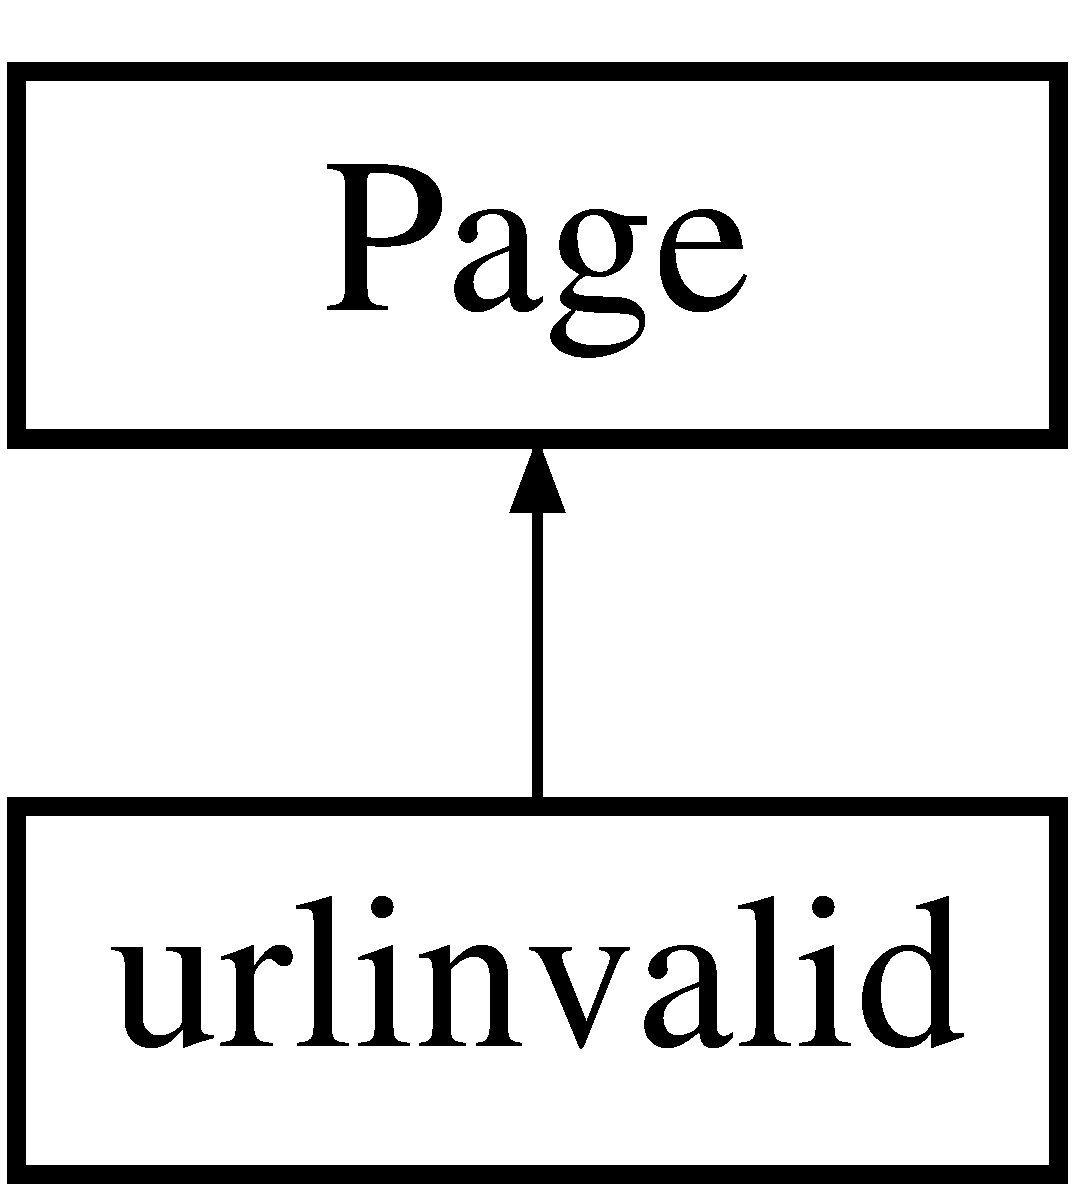
\includegraphics[height=2.000000cm]{classurlinvalid}
\end{center}
\end{figure}
\subsection*{Protected Member Functions}
\begin{DoxyCompactItemize}
\item 
\hypertarget{classurlinvalid_a86a82bd93ece5fdd33c184ba00155264}{void {\bfseries Page\-\_\-\-Load} (object sender, Event\-Args e)}\label{classurlinvalid_a86a82bd93ece5fdd33c184ba00155264}

\end{DoxyCompactItemize}


\subsection{Detailed Description}


Definition at line 8 of file urlinvalid.\-aspx.\-cs.



The documentation for this class was generated from the following file\-:\begin{DoxyCompactItemize}
\item 
E\-:/\-Mint/\-Home care/\-Smart\-Home\-Care/urlinvalid.\-aspx.\-cs\end{DoxyCompactItemize}

\hypertarget{classuseraccountdetails}{\section{useraccountdetails Class Reference}
\label{classuseraccountdetails}\index{useraccountdetails@{useraccountdetails}}
}
Inheritance diagram for useraccountdetails\-:\begin{figure}[H]
\begin{center}
\leavevmode
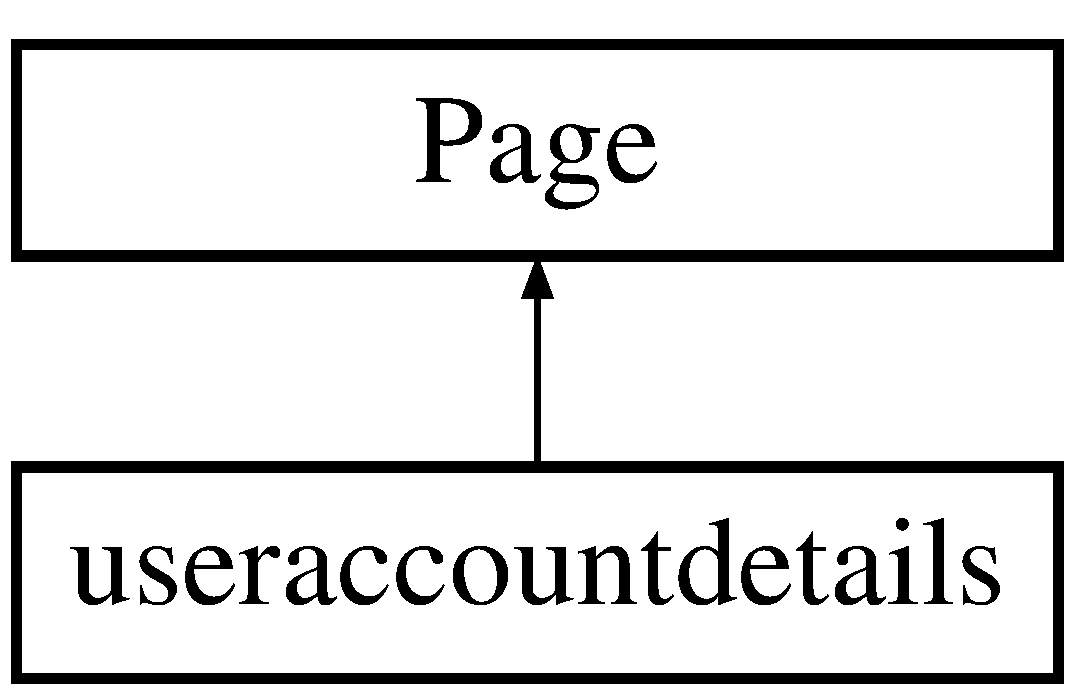
\includegraphics[height=2.000000cm]{classuseraccountdetails}
\end{center}
\end{figure}
\subsection*{Protected Member Functions}
\begin{DoxyCompactItemize}
\item 
\hypertarget{classuseraccountdetails_a38a632cbcb82d51c5619b58a45a1ade3}{void {\bfseries Page\-\_\-\-Load} (object sender, Event\-Args e)}\label{classuseraccountdetails_a38a632cbcb82d51c5619b58a45a1ade3}

\end{DoxyCompactItemize}


\subsection{Detailed Description}


Definition at line 8 of file useraccountdetails.\-aspx.\-cs.



The documentation for this class was generated from the following file\-:\begin{DoxyCompactItemize}
\item 
E\-:/\-Mint/\-Home care/\-Smart\-Home\-Care/useraccountdetails.\-aspx.\-cs\end{DoxyCompactItemize}

\hypertarget{classuseralarmmessages}{\section{useralarmmessages Class Reference}
\label{classuseralarmmessages}\index{useralarmmessages@{useralarmmessages}}
}
Inheritance diagram for useralarmmessages\-:\begin{figure}[H]
\begin{center}
\leavevmode
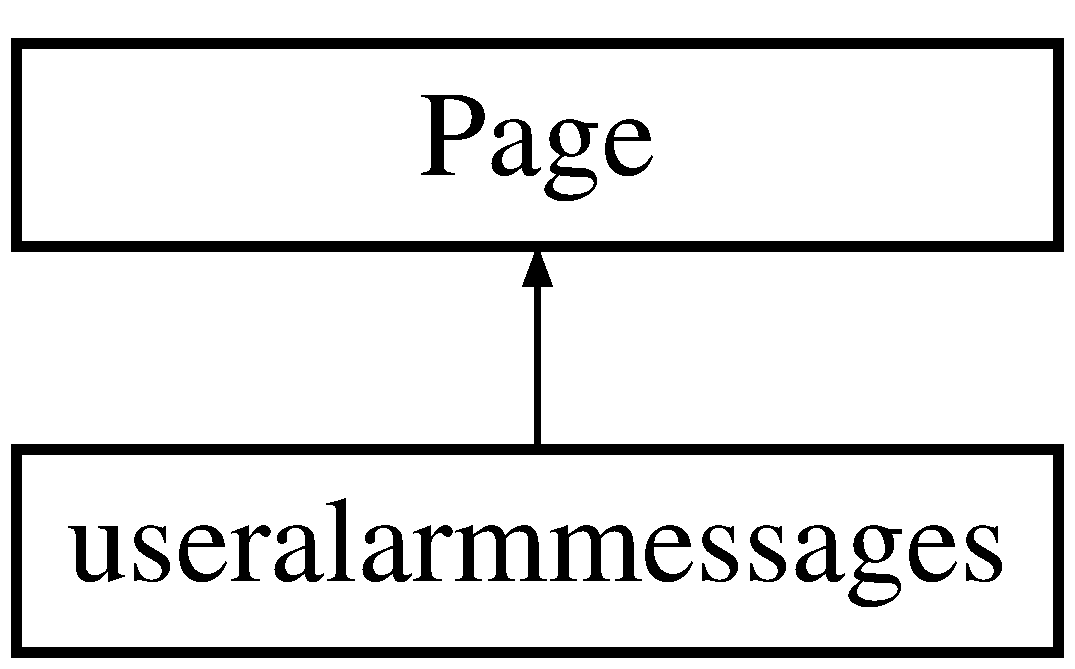
\includegraphics[height=2.000000cm]{classuseralarmmessages}
\end{center}
\end{figure}
\subsection*{Protected Member Functions}
\begin{DoxyCompactItemize}
\item 
\hypertarget{classuseralarmmessages_abced9091eec5a5bf2f615fb82c8ee6f6}{void {\bfseries Page\-\_\-\-Load} (object sender, Event\-Args e)}\label{classuseralarmmessages_abced9091eec5a5bf2f615fb82c8ee6f6}

\end{DoxyCompactItemize}


\subsection{Detailed Description}


Definition at line 9 of file useralarmmessages.\-aspx.\-cs.



The documentation for this class was generated from the following file\-:\begin{DoxyCompactItemize}
\item 
E\-:/\-Mint/\-Home care/\-Smart\-Home\-Care/useralarmmessages.\-aspx.\-cs\end{DoxyCompactItemize}

\hypertarget{classuserauthorizedusers}{\section{userauthorizedusers Class Reference}
\label{classuserauthorizedusers}\index{userauthorizedusers@{userauthorizedusers}}
}
Inheritance diagram for userauthorizedusers\-:\begin{figure}[H]
\begin{center}
\leavevmode
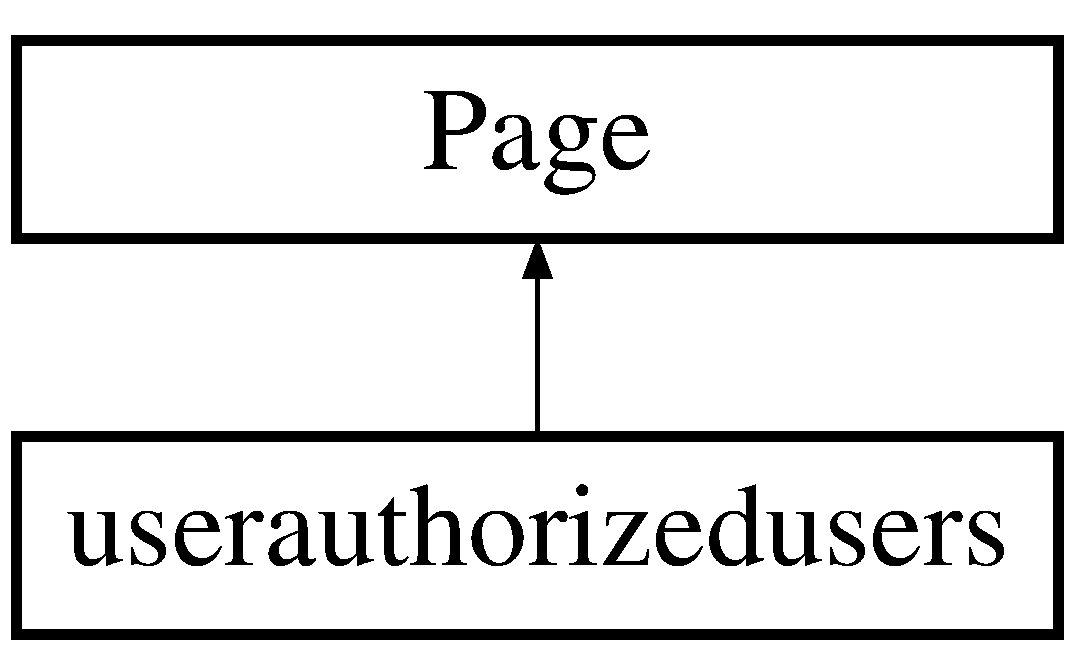
\includegraphics[height=2.000000cm]{classuserauthorizedusers}
\end{center}
\end{figure}
\subsection*{Static Public Member Functions}
\begin{DoxyCompactItemize}
\item 
\hypertarget{classuserauthorizedusers_ae78ced84d8ddee83a25a6fb12f67961a}{static bool {\bfseries User\-Name\-Checker} (string username)}\label{classuserauthorizedusers_ae78ced84d8ddee83a25a6fb12f67961a}

\item 
\hypertarget{classuserauthorizedusers_ae560999e231106ac25eb3741b5ec7220}{static bool {\bfseries Email\-Checker} (string email)}\label{classuserauthorizedusers_ae560999e231106ac25eb3741b5ec7220}

\end{DoxyCompactItemize}
\subsection*{Protected Member Functions}
\begin{DoxyCompactItemize}
\item 
\hypertarget{classuserauthorizedusers_a18be3c06e0da73889a018a2700f31486}{void {\bfseries Page\-\_\-\-Load} (object sender, Event\-Args e)}\label{classuserauthorizedusers_a18be3c06e0da73889a018a2700f31486}

\item 
\hypertarget{classuserauthorizedusers_afa879b631de00b17a7302cb05c27be3e}{void {\bfseries btndelete\-\_\-\-Click} (object sender, Event\-Args e)}\label{classuserauthorizedusers_afa879b631de00b17a7302cb05c27be3e}

\item 
\hypertarget{classuserauthorizedusers_aa9d33cb9d8c5b6e0fe1a518b670bcab5}{void {\bfseries btnadd\-\_\-\-Click} (object sender, Event\-Args e)}\label{classuserauthorizedusers_aa9d33cb9d8c5b6e0fe1a518b670bcab5}

\item 
\hypertarget{classuserauthorizedusers_a0ff994f3a30f20212e2ee83de21e9c4a}{void {\bfseries btninvite\-\_\-\-Click} (object sender, Event\-Args e)}\label{classuserauthorizedusers_a0ff994f3a30f20212e2ee83de21e9c4a}

\end{DoxyCompactItemize}


\subsection{Detailed Description}


Definition at line 10 of file userauthorizedusers.\-aspx.\-cs.



The documentation for this class was generated from the following file\-:\begin{DoxyCompactItemize}
\item 
E\-:/\-Mint/\-Home care/\-Smart\-Home\-Care/userauthorizedusers.\-aspx.\-cs\end{DoxyCompactItemize}

\hypertarget{classuserbillingaccountsummar}{\section{userbillingaccountsummar Class Reference}
\label{classuserbillingaccountsummar}\index{userbillingaccountsummar@{userbillingaccountsummar}}
}
Inheritance diagram for userbillingaccountsummar\-:\begin{figure}[H]
\begin{center}
\leavevmode
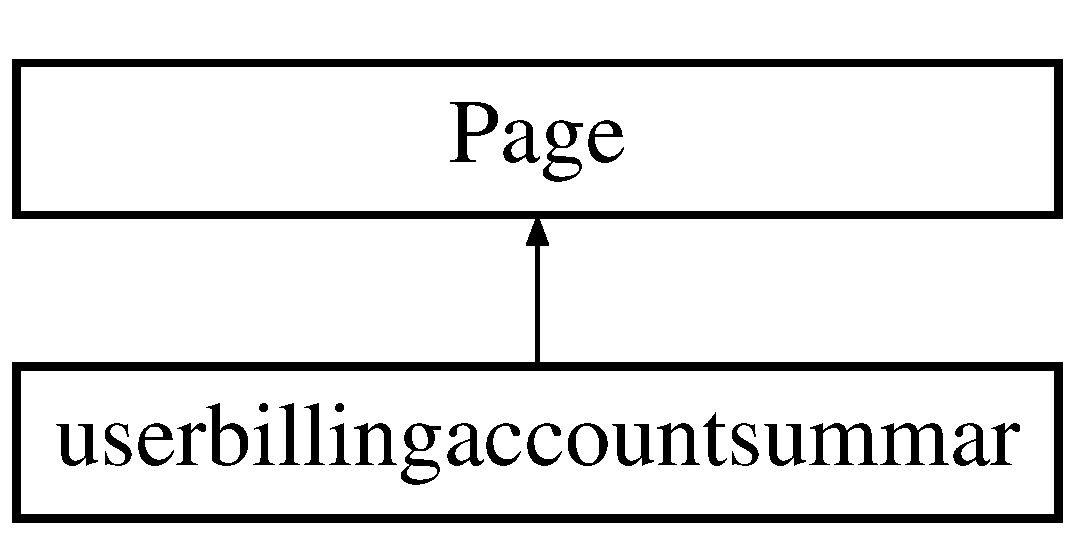
\includegraphics[height=2.000000cm]{classuserbillingaccountsummar}
\end{center}
\end{figure}
\subsection*{Protected Member Functions}
\begin{DoxyCompactItemize}
\item 
\hypertarget{classuserbillingaccountsummar_aae24de1f8e604fcf40f240c563da6fc0}{void {\bfseries Page\-\_\-\-Load} (object sender, Event\-Args e)}\label{classuserbillingaccountsummar_aae24de1f8e604fcf40f240c563da6fc0}

\item 
\hypertarget{classuserbillingaccountsummar_a4eade8d56a011431131bfa213daa2578}{void {\bfseries btnseemorepayments\-\_\-\-Click} (object sender, Event\-Args e)}\label{classuserbillingaccountsummar_a4eade8d56a011431131bfa213daa2578}

\end{DoxyCompactItemize}


\subsection{Detailed Description}


Definition at line 8 of file userbillingaccountsummar.\-aspx.\-cs.



The documentation for this class was generated from the following file\-:\begin{DoxyCompactItemize}
\item 
E\-:/\-Mint/\-Home care/\-Smart\-Home\-Care/userbillingaccountsummar.\-aspx.\-cs\end{DoxyCompactItemize}

\hypertarget{classuserchangepassword}{\section{userchangepassword Class Reference}
\label{classuserchangepassword}\index{userchangepassword@{userchangepassword}}
}
Inheritance diagram for userchangepassword\-:\begin{figure}[H]
\begin{center}
\leavevmode
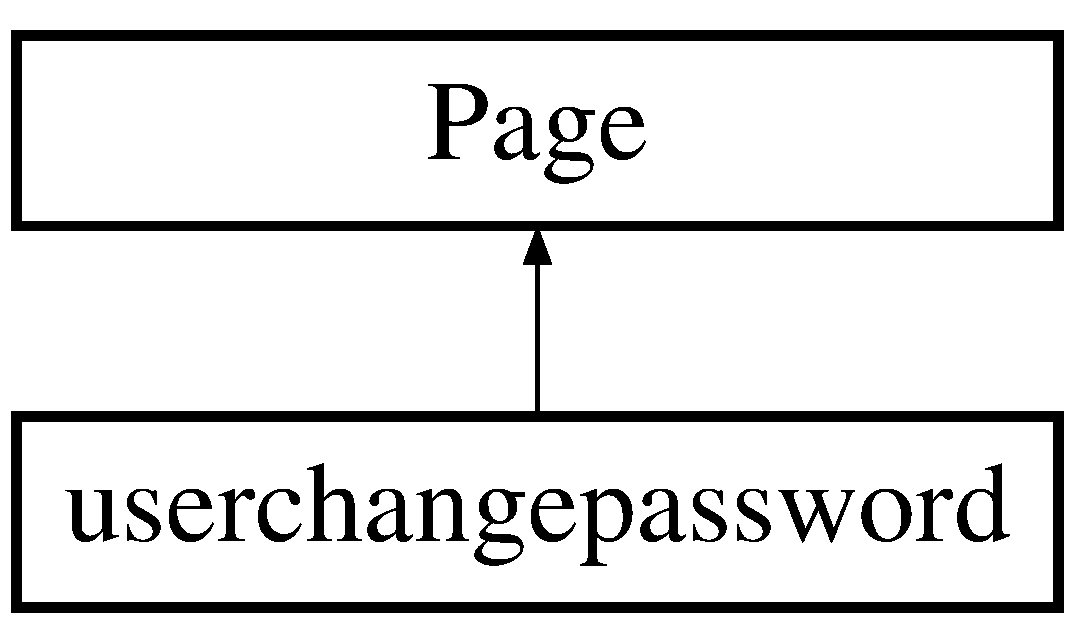
\includegraphics[height=2.000000cm]{classuserchangepassword}
\end{center}
\end{figure}
\subsection*{Protected Member Functions}
\begin{DoxyCompactItemize}
\item 
\hypertarget{classuserchangepassword_a0c49e55a8f1492823751f9a304707ba5}{void {\bfseries Page\-\_\-\-Load} (object sender, Event\-Args e)}\label{classuserchangepassword_a0c49e55a8f1492823751f9a304707ba5}

\item 
\hypertarget{classuserchangepassword_a27261e1143f2269d19db32f93e70d320}{void {\bfseries btnsave\-\_\-\-Click} (object sender, Event\-Args e)}\label{classuserchangepassword_a27261e1143f2269d19db32f93e70d320}

\end{DoxyCompactItemize}


\subsection{Detailed Description}


Definition at line 9 of file userchangepassword.\-aspx.\-cs.



The documentation for this class was generated from the following file\-:\begin{DoxyCompactItemize}
\item 
E\-:/\-Mint/\-Home care/\-Smart\-Home\-Care/userchangepassword.\-aspx.\-cs\end{DoxyCompactItemize}

\hypertarget{classusercompose}{\section{usercompose Class Reference}
\label{classusercompose}\index{usercompose@{usercompose}}
}
Inheritance diagram for usercompose\-:\begin{figure}[H]
\begin{center}
\leavevmode
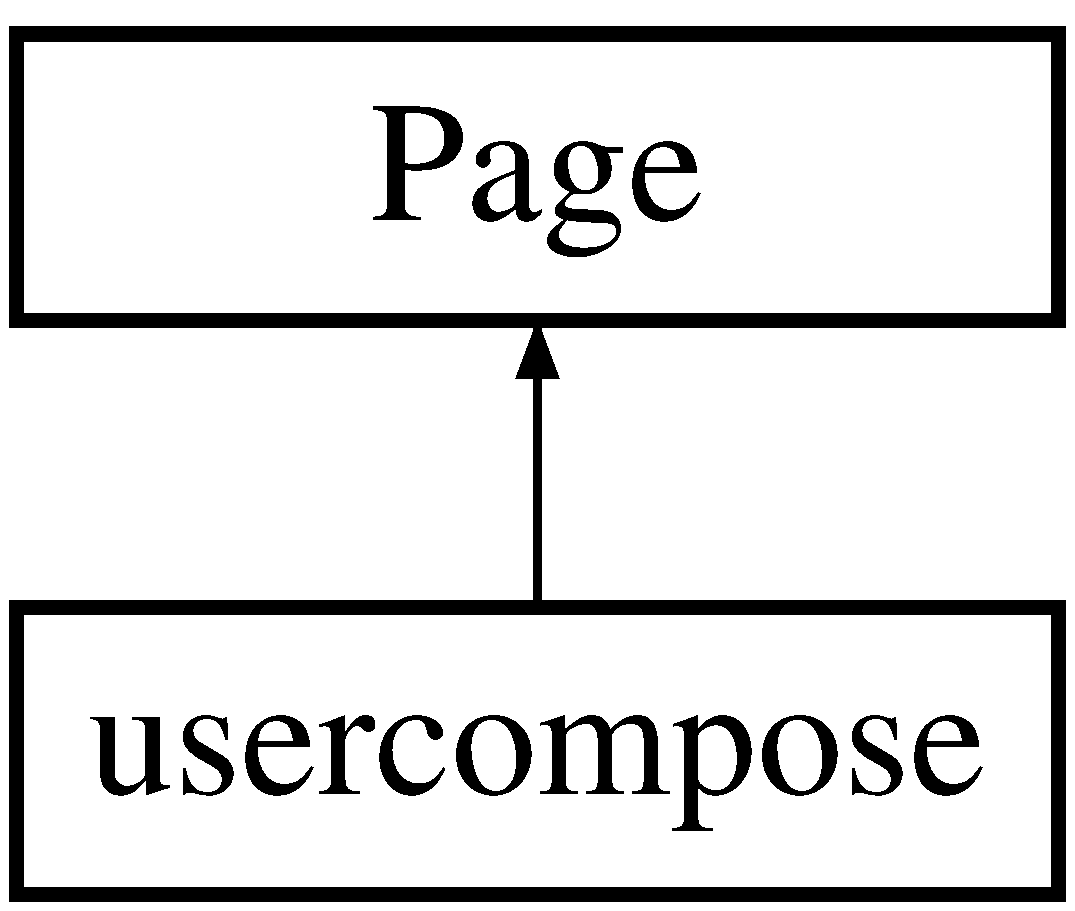
\includegraphics[height=2.000000cm]{classusercompose}
\end{center}
\end{figure}
\subsection*{Static Public Member Functions}
\begin{DoxyCompactItemize}
\item 
\hypertarget{classusercompose_a5d746e6f05e3eeac2c1e01448ade9017}{static object {\bfseries Send\-Mail\-To\-User} (object\mbox{[}$\,$\mbox{]} args)}\label{classusercompose_a5d746e6f05e3eeac2c1e01448ade9017}

\end{DoxyCompactItemize}
\subsection*{Protected Member Functions}
\begin{DoxyCompactItemize}
\item 
\hypertarget{classusercompose_afb83828a828e0ef09530ef29f78afd68}{void {\bfseries Page\-\_\-\-Load} (object sender, Event\-Args e)}\label{classusercompose_afb83828a828e0ef09530ef29f78afd68}

\item 
\hypertarget{classusercompose_a2cfbb63e67c9ec7d69fe6ff26fb5df96}{void {\bfseries btn\-Send\-\_\-\-Click} (object sender, Event\-Args e)}\label{classusercompose_a2cfbb63e67c9ec7d69fe6ff26fb5df96}

\end{DoxyCompactItemize}


\subsection{Detailed Description}
User compose 

Definition at line 12 of file usercompose.\-aspx.\-cs.



The documentation for this class was generated from the following file\-:\begin{DoxyCompactItemize}
\item 
E\-:/\-Mint/\-Home care/\-Smart\-Home\-Care/usercompose.\-aspx.\-cs\end{DoxyCompactItemize}

\hypertarget{classuserhelp}{\section{userhelp Class Reference}
\label{classuserhelp}\index{userhelp@{userhelp}}
}
Inheritance diagram for userhelp\-:\begin{figure}[H]
\begin{center}
\leavevmode
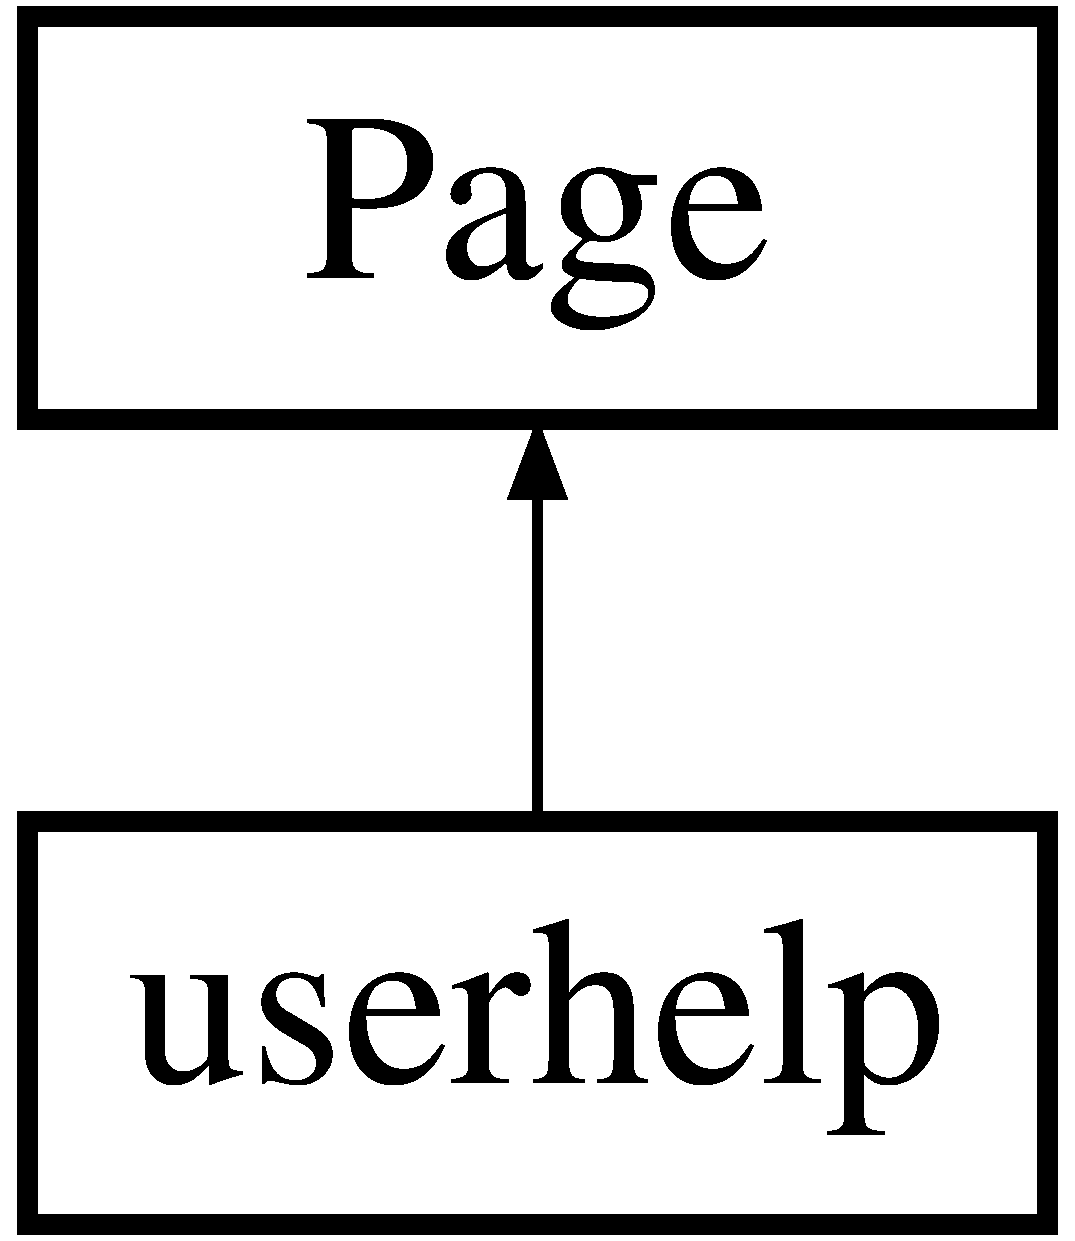
\includegraphics[height=2.000000cm]{classuserhelp}
\end{center}
\end{figure}
\subsection*{Protected Member Functions}
\begin{DoxyCompactItemize}
\item 
\hypertarget{classuserhelp_a2ef8f8b48dd538c14996ecb0a73bc777}{void {\bfseries Page\-\_\-\-Load} (object sender, Event\-Args e)}\label{classuserhelp_a2ef8f8b48dd538c14996ecb0a73bc777}

\end{DoxyCompactItemize}


\subsection{Detailed Description}


Definition at line 8 of file userhelp.\-aspx.\-cs.



The documentation for this class was generated from the following file\-:\begin{DoxyCompactItemize}
\item 
E\-:/\-Mint/\-Home care/\-Smart\-Home\-Care/userhelp.\-aspx.\-cs\end{DoxyCompactItemize}

\hypertarget{classuserhome}{\section{userhome Class Reference}
\label{classuserhome}\index{userhome@{userhome}}
}
Inheritance diagram for userhome\-:\begin{figure}[H]
\begin{center}
\leavevmode
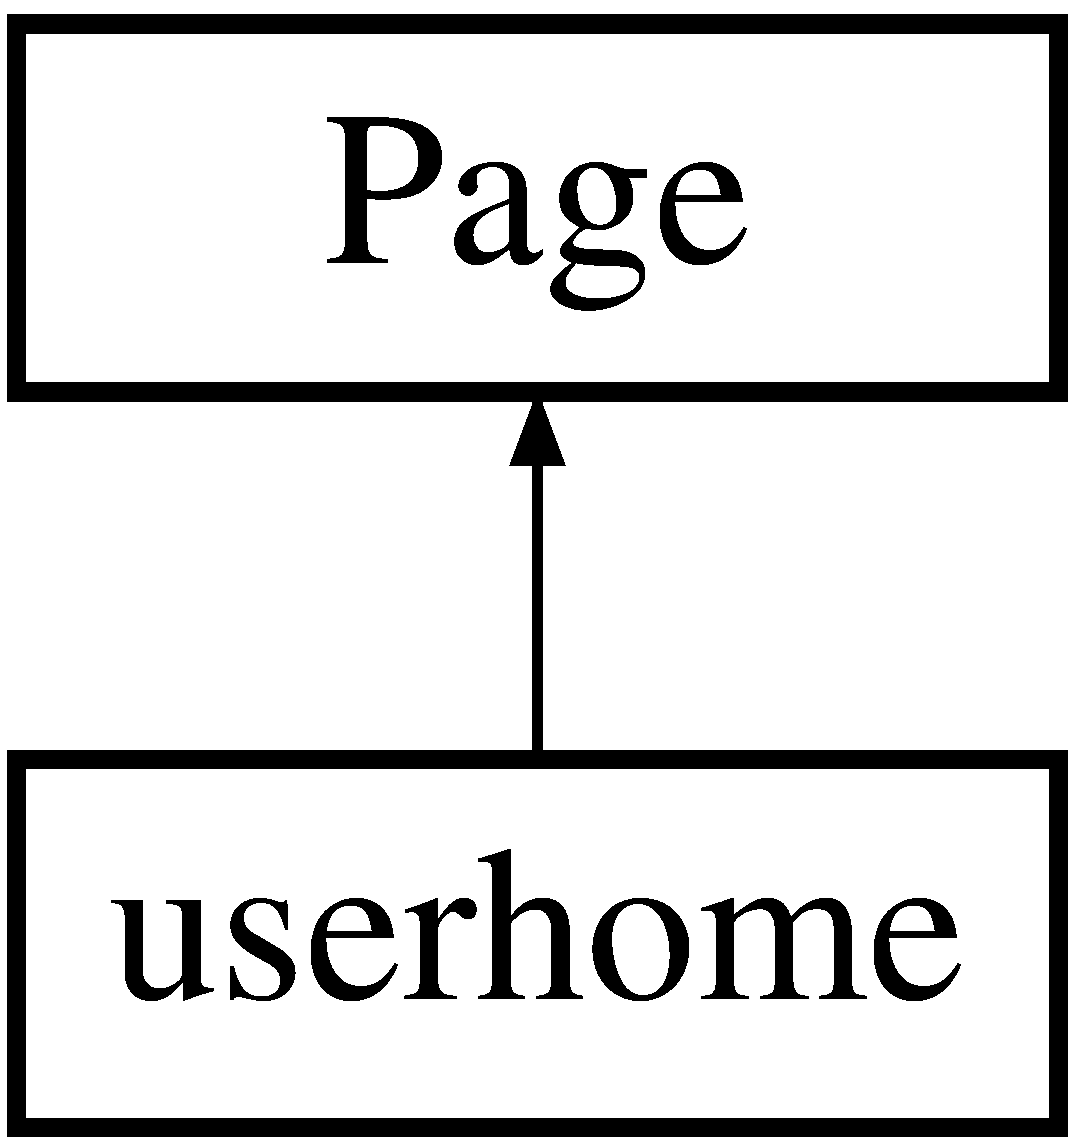
\includegraphics[height=2.000000cm]{classuserhome}
\end{center}
\end{figure}
\subsection*{Protected Member Functions}
\begin{DoxyCompactItemize}
\item 
\hypertarget{classuserhome_a7d5e583242441d72aa4e429048b04d5b}{void {\bfseries Page\-\_\-\-Load} (object sender, Event\-Args e)}\label{classuserhome_a7d5e583242441d72aa4e429048b04d5b}

\end{DoxyCompactItemize}


\subsection{Detailed Description}


Definition at line 9 of file userhome.\-aspx.\-cs.



The documentation for this class was generated from the following file\-:\begin{DoxyCompactItemize}
\item 
E\-:/\-Mint/\-Home care/\-Smart\-Home\-Care/userhome.\-aspx.\-cs\end{DoxyCompactItemize}

\hypertarget{classuserinbox}{\section{userinbox Class Reference}
\label{classuserinbox}\index{userinbox@{userinbox}}
}


Day la mo ta ngan.  


Inheritance diagram for userinbox\-:\begin{figure}[H]
\begin{center}
\leavevmode
\includegraphics[height=2.000000cm]{classuserinbox}
\end{center}
\end{figure}
\subsection*{Static Public Member Functions}
\begin{DoxyCompactItemize}
\item 
\hypertarget{classuserinbox_ab908d29d9645df1b0d4d17804ed98187}{static object {\bfseries Read\-Message} (int id)}\label{classuserinbox_ab908d29d9645df1b0d4d17804ed98187}

\item 
\hypertarget{classuserinbox_a90442e645e1cf5ca2df0b48a10523643}{static object {\bfseries Delete\-Message} (object args)}\label{classuserinbox_a90442e645e1cf5ca2df0b48a10523643}

\end{DoxyCompactItemize}
\subsection*{Protected Member Functions}
\begin{DoxyCompactItemize}
\item 
\hypertarget{classuserinbox_aaab2951d914fead1a10d650c4192aa93}{void {\bfseries Page\-\_\-\-Load} (object sender, Event\-Args e)}\label{classuserinbox_aaab2951d914fead1a10d650c4192aa93}

\item 
void \hyperlink{classuserinbox_a7394a38738fffadb36fc01755032a558}{btndelete\-\_\-\-Click} (object sender, Event\-Args e)
\item 
\hypertarget{classuserinbox_aced870e74070eaecbe627fa149753782}{void {\bfseries Link\-Button2\-\_\-\-Click} (object sender, Event\-Args e)}\label{classuserinbox_aced870e74070eaecbe627fa149753782}

\item 
\hypertarget{classuserinbox_a28e70d6aede9e3784c2146f81ace7cc8}{void {\bfseries lb\-Pre\-\_\-\-Click} (object sender, Event\-Args e)}\label{classuserinbox_a28e70d6aede9e3784c2146f81ace7cc8}

\end{DoxyCompactItemize}


\subsection{Detailed Description}
Day la mo ta ngan. 

Day la mo ta chi tiet 

Definition at line 13 of file userinbox.\-aspx.\-cs.



\subsection{Member Function Documentation}
\hypertarget{classuserinbox_a7394a38738fffadb36fc01755032a558}{\index{userinbox@{userinbox}!btndelete\-\_\-\-Click@{btndelete\-\_\-\-Click}}
\index{btndelete\-\_\-\-Click@{btndelete\-\_\-\-Click}!userinbox@{userinbox}}
\subsubsection[{btndelete\-\_\-\-Click}]{\setlength{\rightskip}{0pt plus 5cm}void userinbox.\-btndelete\-\_\-\-Click (
\begin{DoxyParamCaption}
\item[{object}]{sender, }
\item[{Event\-Args}]{e}
\end{DoxyParamCaption}
)\hspace{0.3cm}{\ttfamily [protected]}}}\label{classuserinbox_a7394a38738fffadb36fc01755032a558}
\mbox{[}Delete\mbox{]} delete messages. 

Definition at line 56 of file userinbox.\-aspx.\-cs.



The documentation for this class was generated from the following file\-:\begin{DoxyCompactItemize}
\item 
E\-:/\-Mint/\-Home care/\-Smart\-Home\-Care/userinbox.\-aspx.\-cs\end{DoxyCompactItemize}

\hypertarget{classuserinformation}{\section{userinformation Class Reference}
\label{classuserinformation}\index{userinformation@{userinformation}}
}
Inheritance diagram for userinformation\-:\begin{figure}[H]
\begin{center}
\leavevmode
\includegraphics[height=2.000000cm]{classuserinformation}
\end{center}
\end{figure}
\subsection*{Protected Member Functions}
\begin{DoxyCompactItemize}
\item 
\hypertarget{classuserinformation_af734bdeedf61434bf29d9b46e726441f}{void {\bfseries Page\-\_\-\-Load} (object sender, Event\-Args e)}\label{classuserinformation_af734bdeedf61434bf29d9b46e726441f}

\item 
\hypertarget{classuserinformation_abefd1ef81db769790bb7f640904e5fe0}{void {\bfseries btnedit\-\_\-\-Click} (object sender, Event\-Args e)}\label{classuserinformation_abefd1ef81db769790bb7f640904e5fe0}

\item 
\hypertarget{classuserinformation_aa72cef6398fd3329922eae4d52b0dbc4}{void {\bfseries btncancel\-\_\-\-Click} (object sender, Event\-Args e)}\label{classuserinformation_aa72cef6398fd3329922eae4d52b0dbc4}

\item 
\hypertarget{classuserinformation_a160472f63ab0e477801d7487b17bc8c3}{void {\bfseries btnsave\-\_\-\-Click} (object sender, Event\-Args e)}\label{classuserinformation_a160472f63ab0e477801d7487b17bc8c3}

\item 
\hypertarget{classuserinformation_a0a7378ba5f44aa56cf0d8e39fcbe3148}{void {\bfseries ddlcountry\-\_\-\-Selected\-Index\-Changed} (object sender, Event\-Args e)}\label{classuserinformation_a0a7378ba5f44aa56cf0d8e39fcbe3148}

\item 
\hypertarget{classuserinformation_aeac9885957c5edd5640438e5cacd7987}{void {\bfseries ddlstate\-\_\-\-Selected\-Index\-Changed} (object sender, Event\-Args e)}\label{classuserinformation_aeac9885957c5edd5640438e5cacd7987}

\end{DoxyCompactItemize}


\subsection{Detailed Description}


Definition at line 9 of file userinformation.\-aspx.\-cs.



The documentation for this class was generated from the following file\-:\begin{DoxyCompactItemize}
\item 
E\-:/\-Mint/\-Home care/\-Smart\-Home\-Care/userinformation.\-aspx.\-cs\end{DoxyCompactItemize}

\hypertarget{classuserpaybill}{\section{userpaybill Class Reference}
\label{classuserpaybill}\index{userpaybill@{userpaybill}}
}
Inheritance diagram for userpaybill\-:\begin{figure}[H]
\begin{center}
\leavevmode
\includegraphics[height=2.000000cm]{classuserpaybill}
\end{center}
\end{figure}
\subsection*{Protected Member Functions}
\begin{DoxyCompactItemize}
\item 
\hypertarget{classuserpaybill_af3752c51efa020ea2d960f42c1b40b79}{void {\bfseries Page\-\_\-\-Load} (object sender, Event\-Args e)}\label{classuserpaybill_af3752c51efa020ea2d960f42c1b40b79}

\item 
\hypertarget{classuserpaybill_af290c6f29a7c4fbc8a32a332f6c31dc9}{void {\bfseries btncontinue\-\_\-\-Click} (object sender, Event\-Args e)}\label{classuserpaybill_af290c6f29a7c4fbc8a32a332f6c31dc9}

\item 
\hypertarget{classuserpaybill_a7863394c68dd1f4a431daa606d0befe9}{void {\bfseries ddlcountry\-\_\-\-Selected\-Index\-Changed} (object sender, Event\-Args e)}\label{classuserpaybill_a7863394c68dd1f4a431daa606d0befe9}

\item 
\hypertarget{classuserpaybill_af6bbe9beeea71396506c53376195a0e0}{void {\bfseries lbtnprint\-\_\-\-Click} (object sender, Event\-Args e)}\label{classuserpaybill_af6bbe9beeea71396506c53376195a0e0}

\end{DoxyCompactItemize}


\subsection{Detailed Description}


Definition at line 8 of file userpaybill.\-aspx.\-cs.



The documentation for this class was generated from the following file\-:\begin{DoxyCompactItemize}
\item 
E\-:/\-Mint/\-Home care/\-Smart\-Home\-Care/userpaybill.\-aspx.\-cs\end{DoxyCompactItemize}

\hypertarget{classuserpaymentinformation}{\section{userpaymentinformation Class Reference}
\label{classuserpaymentinformation}\index{userpaymentinformation@{userpaymentinformation}}
}
Inheritance diagram for userpaymentinformation\-:\begin{figure}[H]
\begin{center}
\leavevmode
\includegraphics[height=2.000000cm]{classuserpaymentinformation}
\end{center}
\end{figure}
\subsection*{Protected Member Functions}
\begin{DoxyCompactItemize}
\item 
\hypertarget{classuserpaymentinformation_a6f1d2533f356ab449415613755a01726}{void {\bfseries Page\-\_\-\-Load} (object sender, Event\-Args e)}\label{classuserpaymentinformation_a6f1d2533f356ab449415613755a01726}

\item 
\hypertarget{classuserpaymentinformation_af60e50e556720f6883a25026754fd77f}{void {\bfseries grd\-Info\-\_\-\-Row\-Data\-Bound} (object sender, Grid\-View\-Row\-Event\-Args e)}\label{classuserpaymentinformation_af60e50e556720f6883a25026754fd77f}

\end{DoxyCompactItemize}


\subsection{Detailed Description}


Definition at line 8 of file userpaymentinformation.\-aspx.\-cs.



The documentation for this class was generated from the following file\-:\begin{DoxyCompactItemize}
\item 
E\-:/\-Mint/\-Home care/\-Smart\-Home\-Care/userpaymentinformation.\-aspx.\-cs\end{DoxyCompactItemize}

\hypertarget{classuserpaymentreceipt}{\section{userpaymentreceipt Class Reference}
\label{classuserpaymentreceipt}\index{userpaymentreceipt@{userpaymentreceipt}}
}
Inheritance diagram for userpaymentreceipt\-:\begin{figure}[H]
\begin{center}
\leavevmode
\includegraphics[height=2.000000cm]{classuserpaymentreceipt}
\end{center}
\end{figure}
\subsection*{Protected Member Functions}
\begin{DoxyCompactItemize}
\item 
\hypertarget{classuserpaymentreceipt_a36415d33969c5f0f6a3fd9979641f876}{void {\bfseries Page\-\_\-\-Load} (object sender, Event\-Args e)}\label{classuserpaymentreceipt_a36415d33969c5f0f6a3fd9979641f876}

\end{DoxyCompactItemize}


\subsection{Detailed Description}


Definition at line 8 of file userpayment\-\_\-receipt.\-aspx.\-cs.



The documentation for this class was generated from the following file\-:\begin{DoxyCompactItemize}
\item 
E\-:/\-Mint/\-Home care/\-Smart\-Home\-Care/userpayment\-\_\-receipt.\-aspx.\-cs\end{DoxyCompactItemize}

\hypertarget{classuserpaymentreview}{\section{userpaymentreview Class Reference}
\label{classuserpaymentreview}\index{userpaymentreview@{userpaymentreview}}
}
Inheritance diagram for userpaymentreview\-:\begin{figure}[H]
\begin{center}
\leavevmode
\includegraphics[height=2.000000cm]{classuserpaymentreview}
\end{center}
\end{figure}
\subsection*{Protected Member Functions}
\begin{DoxyCompactItemize}
\item 
\hypertarget{classuserpaymentreview_a3fa1f1f4cbf4ceb3494b0906d5aac025}{void {\bfseries Page\-\_\-\-Load} (object sender, Event\-Args e)}\label{classuserpaymentreview_a3fa1f1f4cbf4ceb3494b0906d5aac025}

\item 
\hypertarget{classuserpaymentreview_aa27f759e0079382395155e6b3d2e090a}{void {\bfseries btnsubmit\-\_\-\-Click} (object sender, Event\-Args e)}\label{classuserpaymentreview_aa27f759e0079382395155e6b3d2e090a}

\end{DoxyCompactItemize}


\subsection{Detailed Description}


Definition at line 8 of file userpayment\-\_\-review.\-aspx.\-cs.



The documentation for this class was generated from the following file\-:\begin{DoxyCompactItemize}
\item 
E\-:/\-Mint/\-Home care/\-Smart\-Home\-Care/userpayment\-\_\-review.\-aspx.\-cs\end{DoxyCompactItemize}

\hypertarget{classuserreadmessage}{\section{userreadmessage Class Reference}
\label{classuserreadmessage}\index{userreadmessage@{userreadmessage}}
}
Inheritance diagram for userreadmessage\-:\begin{figure}[H]
\begin{center}
\leavevmode
\includegraphics[height=2.000000cm]{classuserreadmessage}
\end{center}
\end{figure}
\subsection*{Protected Member Functions}
\begin{DoxyCompactItemize}
\item 
\hypertarget{classuserreadmessage_ad26c0053356993eafb3be444be1bf391}{void {\bfseries Page\-\_\-\-Load} (object sender, Event\-Args e)}\label{classuserreadmessage_ad26c0053356993eafb3be444be1bf391}

\end{DoxyCompactItemize}


\subsection{Detailed Description}


Definition at line 8 of file userreadmessage.\-aspx.\-cs.



The documentation for this class was generated from the following file\-:\begin{DoxyCompactItemize}
\item 
E\-:/\-Mint/\-Home care/\-Smart\-Home\-Care/userreadmessage.\-aspx.\-cs\end{DoxyCompactItemize}

\hypertarget{class_users}{\section{Users Class Reference}
\label{class_users}\index{Users@{Users}}
}


property user login website  


\subsection*{Public Attributes}
\begin{DoxyCompactItemize}
\item 
\hypertarget{class_users_af916b787a91eacd25ce0bc12715569ca}{const string {\bfseries M\-O\-N} =\char`\"{}M\-O\-N\char`\"{}}\label{class_users_af916b787a91eacd25ce0bc12715569ca}

\item 
\hypertarget{class_users_a699fc73d2ed83b3cacb51fe85aa72db9}{const string {\bfseries P\-A\-R} = \char`\"{}P\-A\-R\char`\"{}}\label{class_users_a699fc73d2ed83b3cacb51fe85aa72db9}

\item 
\hypertarget{class_users_a118d2f4312f279dc03af9e6a2406b3a1}{const string {\bfseries P\-R\-I} = \char`\"{}P\-R\-I\char`\"{}}\label{class_users_a118d2f4312f279dc03af9e6a2406b3a1}

\end{DoxyCompactItemize}


\subsection{Detailed Description}
property user login website 

Definition at line 9 of file Users.\-cs.



The documentation for this class was generated from the following file\-:\begin{DoxyCompactItemize}
\item 
E\-:/\-Mint/\-Home care/\-Smart\-Home\-Care/\-App\-\_\-\-Code/Users.\-cs\end{DoxyCompactItemize}

\hypertarget{classusersentmessages}{\section{usersentmessages Class Reference}
\label{classusersentmessages}\index{usersentmessages@{usersentmessages}}
}
Inheritance diagram for usersentmessages\-:\begin{figure}[H]
\begin{center}
\leavevmode
\includegraphics[height=2.000000cm]{classusersentmessages}
\end{center}
\end{figure}
\subsection*{Protected Member Functions}
\begin{DoxyCompactItemize}
\item 
\hypertarget{classusersentmessages_ab445f879aefe22399c718a1d919c4ba3}{void {\bfseries Page\-\_\-\-Load} (object sender, Event\-Args e)}\label{classusersentmessages_ab445f879aefe22399c718a1d919c4ba3}

\item 
\hypertarget{classusersentmessages_ab6690e8cbc16e863690db803a17840bc}{void {\bfseries btndelete\-\_\-\-Click} (object sender, Event\-Args e)}\label{classusersentmessages_ab6690e8cbc16e863690db803a17840bc}

\item 
\hypertarget{classusersentmessages_ab19ad9f15af5c332ac4ca01af58b336f}{void {\bfseries Link\-Button2\-\_\-\-Click} (object sender, Event\-Args e)}\label{classusersentmessages_ab19ad9f15af5c332ac4ca01af58b336f}

\item 
\hypertarget{classusersentmessages_a35b3995a84dfa1b34ca86281206f1e1e}{void {\bfseries lb\-Pre\-\_\-\-Click} (object sender, Event\-Args e)}\label{classusersentmessages_a35b3995a84dfa1b34ca86281206f1e1e}

\item 
\hypertarget{classusersentmessages_aa363756e43cab48d0a643c41bdd715c8}{void {\bfseries Link\-Button2\-\_\-\-Click} (object sender, Image\-Click\-Event\-Args e)}\label{classusersentmessages_aa363756e43cab48d0a643c41bdd715c8}

\end{DoxyCompactItemize}


\subsection{Detailed Description}


Definition at line 9 of file usersentmessages.\-aspx.\-cs.



The documentation for this class was generated from the following file\-:\begin{DoxyCompactItemize}
\item 
E\-:/\-Mint/\-Home care/\-Smart\-Home\-Care/usersentmessages.\-aspx.\-cs\end{DoxyCompactItemize}

\hypertarget{classusersitemap}{\section{usersitemap Class Reference}
\label{classusersitemap}\index{usersitemap@{usersitemap}}
}
Inheritance diagram for usersitemap\-:\begin{figure}[H]
\begin{center}
\leavevmode
\includegraphics[height=2.000000cm]{classusersitemap}
\end{center}
\end{figure}
\subsection*{Protected Member Functions}
\begin{DoxyCompactItemize}
\item 
\hypertarget{classusersitemap_ad0202ea231079855724ccc96b1ad6d21}{void {\bfseries Page\-\_\-\-Load} (object sender, Event\-Args e)}\label{classusersitemap_ad0202ea231079855724ccc96b1ad6d21}

\item 
\hypertarget{classusersitemap_ad0202ea231079855724ccc96b1ad6d21}{void {\bfseries Page\-\_\-\-Load} (object sender, Event\-Args e)}\label{classusersitemap_ad0202ea231079855724ccc96b1ad6d21}

\end{DoxyCompactItemize}


\subsection{Detailed Description}


Definition at line 8 of file usersitemap.\-aspx.\-cs.



The documentation for this class was generated from the following files\-:\begin{DoxyCompactItemize}
\item 
E\-:/\-Mint/\-Home care/\-Smart\-Home\-Care/usersitemap.\-aspx.\-cs\item 
E\-:/\-Mint/\-Home care/\-Smart\-Home\-Care/x\-\_\-usersitemap.\-aspx.\-cs\end{DoxyCompactItemize}

\hypertarget{classusertrackmyhealth}{\section{usertrackmyhealth Class Reference}
\label{classusertrackmyhealth}\index{usertrackmyhealth@{usertrackmyhealth}}
}
Inheritance diagram for usertrackmyhealth\-:\begin{figure}[H]
\begin{center}
\leavevmode
\includegraphics[height=2.000000cm]{classusertrackmyhealth}
\end{center}
\end{figure}
\subsection*{Protected Member Functions}
\begin{DoxyCompactItemize}
\item 
\hypertarget{classusertrackmyhealth_a9d9d06e80e496922d11a23f4adbc6423}{void {\bfseries Page\-\_\-\-Load} (object sender, Event\-Args e)}\label{classusertrackmyhealth_a9d9d06e80e496922d11a23f4adbc6423}

\item 
\hypertarget{classusertrackmyhealth_a8a20b35ada54adfa9277a11520a36c67}{void {\bfseries Button1\-\_\-\-Click} (object sender, Event\-Args e)}\label{classusertrackmyhealth_a8a20b35ada54adfa9277a11520a36c67}

\item 
\hypertarget{classusertrackmyhealth_a8e35645b0450655e4e39fa181b7e9519}{void {\bfseries btnglobalsettings\-\_\-\-Click} (object sender, Event\-Args e)}\label{classusertrackmyhealth_a8e35645b0450655e4e39fa181b7e9519}

\item 
\hypertarget{classusertrackmyhealth_a43a839dc34bcab7c2f8e0f365990e222}{void {\bfseries ibtn\-\_\-\-Click} (object sender, Image\-Click\-Event\-Args e)}\label{classusertrackmyhealth_a43a839dc34bcab7c2f8e0f365990e222}

\item 
\hypertarget{classusertrackmyhealth_aff47432c6297139f01173ba082fcda14}{void {\bfseries Image\-Button1\-\_\-\-Click} (object sender, Image\-Click\-Event\-Args e)}\label{classusertrackmyhealth_aff47432c6297139f01173ba082fcda14}

\item 
\hypertarget{classusertrackmyhealth_a9d9d06e80e496922d11a23f4adbc6423}{void {\bfseries Page\-\_\-\-Load} (object sender, Event\-Args e)}\label{classusertrackmyhealth_a9d9d06e80e496922d11a23f4adbc6423}

\item 
\hypertarget{classusertrackmyhealth_a8e35645b0450655e4e39fa181b7e9519}{void {\bfseries btnglobalsettings\-\_\-\-Click} (object sender, Event\-Args e)}\label{classusertrackmyhealth_a8e35645b0450655e4e39fa181b7e9519}

\item 
\hypertarget{classusertrackmyhealth_a1fccd745e74228ab3119d1443de69dee}{void {\bfseries ibtn\-\_\-\-Click1} (object sender, Image\-Click\-Event\-Args e)}\label{classusertrackmyhealth_a1fccd745e74228ab3119d1443de69dee}

\end{DoxyCompactItemize}


\subsection{Detailed Description}


Definition at line 9 of file usertrackmyhealth.\-aspx.\-cs.



The documentation for this class was generated from the following files\-:\begin{DoxyCompactItemize}
\item 
E\-:/\-Mint/\-Home care/\-Smart\-Home\-Care/usertrackmyhealth.\-aspx.\-cs\item 
E\-:/\-Mint/\-Home care/\-Smart\-Home\-Care/usertrackotherhealth.\-aspx.\-cs\end{DoxyCompactItemize}

\hypertarget{classusertrackmyhealth__bodymeasurement}{\section{usertrackmyhealth\-\_\-bodymeasurement Class Reference}
\label{classusertrackmyhealth__bodymeasurement}\index{usertrackmyhealth\-\_\-bodymeasurement@{usertrackmyhealth\-\_\-bodymeasurement}}
}
Inheritance diagram for usertrackmyhealth\-\_\-bodymeasurement\-:\begin{figure}[H]
\begin{center}
\leavevmode
\includegraphics[height=2.000000cm]{classusertrackmyhealth__bodymeasurement}
\end{center}
\end{figure}
\subsection*{Protected Member Functions}
\begin{DoxyCompactItemize}
\item 
\hypertarget{classusertrackmyhealth__bodymeasurement_aa7aa3928ae1b1230cc3ad2cc8e24e05b}{void {\bfseries Page\-\_\-\-Load} (object sender, Event\-Args e)}\label{classusertrackmyhealth__bodymeasurement_aa7aa3928ae1b1230cc3ad2cc8e24e05b}

\item 
\hypertarget{classusertrackmyhealth__bodymeasurement_a0f7be178c259b0f7963c753f26520305}{void {\bfseries btn\-Graph2\-\_\-\-Click} (object sender, Event\-Args e)}\label{classusertrackmyhealth__bodymeasurement_a0f7be178c259b0f7963c753f26520305}

\item 
\hypertarget{classusertrackmyhealth__bodymeasurement_a8b0019e124c30c6ba41662982ec1a89a}{void {\bfseries btn\-Table2\-\_\-\-Click} (object sender, Event\-Args e)}\label{classusertrackmyhealth__bodymeasurement_a8b0019e124c30c6ba41662982ec1a89a}

\item 
\hypertarget{classusertrackmyhealth__bodymeasurement_a8ca108cb6651d5f593b6a91920ebefb3}{void {\bfseries grv\-Temp\-\_\-\-Page\-Index\-Changing} (object sender, Grid\-View\-Page\-Event\-Args e)}\label{classusertrackmyhealth__bodymeasurement_a8ca108cb6651d5f593b6a91920ebefb3}

\item 
\hypertarget{classusertrackmyhealth__bodymeasurement_a1ce85222922590c4ff246745e1338a98}{void {\bfseries Button1\-\_\-\-Click} (object sender, Event\-Args e)}\label{classusertrackmyhealth__bodymeasurement_a1ce85222922590c4ff246745e1338a98}

\item 
\hypertarget{classusertrackmyhealth__bodymeasurement_afea29cbb91d8dabcab9e58775f0680ce}{void {\bfseries btn\-Ok\-\_\-\-Click} (object sender, Event\-Args e)}\label{classusertrackmyhealth__bodymeasurement_afea29cbb91d8dabcab9e58775f0680ce}

\item 
void \hyperlink{classusertrackmyhealth__bodymeasurement_ae47ccc516acfc1d3235d82a599f9fb13}{btn\-View\-\_\-\-Click} (object sender, Event\-Args e)
\item 
void \hyperlink{classusertrackmyhealth__bodymeasurement_af416738243f4bda3b98c9cd16171092c}{btn\-\_\-\-Ok\-\_\-\-Table\-\_\-\-Click} (object sender, Event\-Args e)
\item 
void \hyperlink{classusertrackmyhealth__bodymeasurement_aadb7f96211a16c80b41a03f72323248d}{btncancel2\-\_\-\-Click} (object sender, Event\-Args e)
\item 
void \hyperlink{classusertrackmyhealth__bodymeasurement_ae1b1b7bca651bc9da75a752765f5337d}{lb\-Date\-Table\-\_\-\-Click} (object sender, Event\-Args e)
\item 
void \hyperlink{classusertrackmyhealth__bodymeasurement_adbe428fe5ca4fc3590503d43da70e919}{btn\-Cancel\-\_\-\-Click} (object sender, Event\-Args e)
\item 
void \hyperlink{classusertrackmyhealth__bodymeasurement_a7d9b2f1ba757b79680d81aa832b1ea53}{lbtn\-Date\-Time\-\_\-\-Click} (object sender, Event\-Args e)
\item 
\hypertarget{classusertrackmyhealth__bodymeasurement_aa7aa3928ae1b1230cc3ad2cc8e24e05b}{void {\bfseries Page\-\_\-\-Load} (object sender, Event\-Args e)}\label{classusertrackmyhealth__bodymeasurement_aa7aa3928ae1b1230cc3ad2cc8e24e05b}

\item 
\hypertarget{classusertrackmyhealth__bodymeasurement_a0f7be178c259b0f7963c753f26520305}{void {\bfseries btn\-Graph2\-\_\-\-Click} (object sender, Event\-Args e)}\label{classusertrackmyhealth__bodymeasurement_a0f7be178c259b0f7963c753f26520305}

\item 
\hypertarget{classusertrackmyhealth__bodymeasurement_a8b0019e124c30c6ba41662982ec1a89a}{void {\bfseries btn\-Table2\-\_\-\-Click} (object sender, Event\-Args e)}\label{classusertrackmyhealth__bodymeasurement_a8b0019e124c30c6ba41662982ec1a89a}

\item 
\hypertarget{classusertrackmyhealth__bodymeasurement_a8ca108cb6651d5f593b6a91920ebefb3}{void {\bfseries grv\-Temp\-\_\-\-Page\-Index\-Changing} (object sender, Grid\-View\-Page\-Event\-Args e)}\label{classusertrackmyhealth__bodymeasurement_a8ca108cb6651d5f593b6a91920ebefb3}

\item 
\hypertarget{classusertrackmyhealth__bodymeasurement_a95d53c3f78a4373f73d61ddbfdbe94b5}{void {\bfseries btn\-Filter\-\_\-\-Click} (object sender, Event\-Args e)}\label{classusertrackmyhealth__bodymeasurement_a95d53c3f78a4373f73d61ddbfdbe94b5}

\item 
\hypertarget{classusertrackmyhealth__bodymeasurement_a1ce85222922590c4ff246745e1338a98}{void {\bfseries Button1\-\_\-\-Click} (object sender, Event\-Args e)}\label{classusertrackmyhealth__bodymeasurement_a1ce85222922590c4ff246745e1338a98}

\item 
\hypertarget{classusertrackmyhealth__bodymeasurement_afea29cbb91d8dabcab9e58775f0680ce}{void {\bfseries btn\-Ok\-\_\-\-Click} (object sender, Event\-Args e)}\label{classusertrackmyhealth__bodymeasurement_afea29cbb91d8dabcab9e58775f0680ce}

\item 
\hypertarget{classusertrackmyhealth__bodymeasurement_ae47ccc516acfc1d3235d82a599f9fb13}{void {\bfseries btn\-View\-\_\-\-Click} (object sender, Event\-Args e)}\label{classusertrackmyhealth__bodymeasurement_ae47ccc516acfc1d3235d82a599f9fb13}

\item 
\hypertarget{classusertrackmyhealth__bodymeasurement_abae31dc0fccc121c6765a7623c3b5ba5}{void {\bfseries btn\-Next\-\_\-\-Click} (object sender, Event\-Args e)}\label{classusertrackmyhealth__bodymeasurement_abae31dc0fccc121c6765a7623c3b5ba5}

\item 
\hypertarget{classusertrackmyhealth__bodymeasurement_ac78e7bf083ecd024cb4be2535fa5be32}{void {\bfseries btn\-\_\-back\-\_\-\-Click} (object sender, Event\-Args e)}\label{classusertrackmyhealth__bodymeasurement_ac78e7bf083ecd024cb4be2535fa5be32}

\end{DoxyCompactItemize}


\subsection{Detailed Description}


Definition at line 12 of file usertrackmyhealth\-\_\-bodymeasurement.\-aspx.\-cs.



\subsection{Member Function Documentation}
\hypertarget{classusertrackmyhealth__bodymeasurement_af416738243f4bda3b98c9cd16171092c}{\index{usertrackmyhealth\-\_\-bodymeasurement@{usertrackmyhealth\-\_\-bodymeasurement}!btn\-\_\-\-Ok\-\_\-\-Table\-\_\-\-Click@{btn\-\_\-\-Ok\-\_\-\-Table\-\_\-\-Click}}
\index{btn\-\_\-\-Ok\-\_\-\-Table\-\_\-\-Click@{btn\-\_\-\-Ok\-\_\-\-Table\-\_\-\-Click}!usertrackmyhealth_bodymeasurement@{usertrackmyhealth\-\_\-bodymeasurement}}
\subsubsection[{btn\-\_\-\-Ok\-\_\-\-Table\-\_\-\-Click}]{\setlength{\rightskip}{0pt plus 5cm}void usertrackmyhealth\-\_\-bodymeasurement.\-btn\-\_\-\-Ok\-\_\-\-Table\-\_\-\-Click (
\begin{DoxyParamCaption}
\item[{object}]{sender, }
\item[{Event\-Args}]{e}
\end{DoxyParamCaption}
)\hspace{0.3cm}{\ttfamily [protected]}}}\label{classusertrackmyhealth__bodymeasurement_af416738243f4bda3b98c9cd16171092c}
\mbox{[}Filter for table report\mbox{]}Filter data with datetime selected. 

Definition at line 315 of file usertrackmyhealth\-\_\-bodymeasurement.\-aspx.\-cs.

\hypertarget{classusertrackmyhealth__bodymeasurement_aadb7f96211a16c80b41a03f72323248d}{\index{usertrackmyhealth\-\_\-bodymeasurement@{usertrackmyhealth\-\_\-bodymeasurement}!btncancel2\-\_\-\-Click@{btncancel2\-\_\-\-Click}}
\index{btncancel2\-\_\-\-Click@{btncancel2\-\_\-\-Click}!usertrackmyhealth_bodymeasurement@{usertrackmyhealth\-\_\-bodymeasurement}}
\subsubsection[{btncancel2\-\_\-\-Click}]{\setlength{\rightskip}{0pt plus 5cm}void usertrackmyhealth\-\_\-bodymeasurement.\-btncancel2\-\_\-\-Click (
\begin{DoxyParamCaption}
\item[{object}]{sender, }
\item[{Event\-Args}]{e}
\end{DoxyParamCaption}
)\hspace{0.3cm}{\ttfamily [protected]}}}\label{classusertrackmyhealth__bodymeasurement_aadb7f96211a16c80b41a03f72323248d}
\mbox{[}Cancel\mbox{]} click -\/$>$ popup datetime table close. 

Definition at line 324 of file usertrackmyhealth\-\_\-bodymeasurement.\-aspx.\-cs.

\hypertarget{classusertrackmyhealth__bodymeasurement_adbe428fe5ca4fc3590503d43da70e919}{\index{usertrackmyhealth\-\_\-bodymeasurement@{usertrackmyhealth\-\_\-bodymeasurement}!btn\-Cancel\-\_\-\-Click@{btn\-Cancel\-\_\-\-Click}}
\index{btn\-Cancel\-\_\-\-Click@{btn\-Cancel\-\_\-\-Click}!usertrackmyhealth_bodymeasurement@{usertrackmyhealth\-\_\-bodymeasurement}}
\subsubsection[{btn\-Cancel\-\_\-\-Click}]{\setlength{\rightskip}{0pt plus 5cm}void usertrackmyhealth\-\_\-bodymeasurement.\-btn\-Cancel\-\_\-\-Click (
\begin{DoxyParamCaption}
\item[{object}]{sender, }
\item[{Event\-Args}]{e}
\end{DoxyParamCaption}
)\hspace{0.3cm}{\ttfamily [protected]}}}\label{classusertrackmyhealth__bodymeasurement_adbe428fe5ca4fc3590503d43da70e919}
\mbox{[}Cancel\mbox{]} click -\/$>$ popup datetime graph close. 

Definition at line 338 of file usertrackmyhealth\-\_\-bodymeasurement.\-aspx.\-cs.

\hypertarget{classusertrackmyhealth__bodymeasurement_ae47ccc516acfc1d3235d82a599f9fb13}{\index{usertrackmyhealth\-\_\-bodymeasurement@{usertrackmyhealth\-\_\-bodymeasurement}!btn\-View\-\_\-\-Click@{btn\-View\-\_\-\-Click}}
\index{btn\-View\-\_\-\-Click@{btn\-View\-\_\-\-Click}!usertrackmyhealth_bodymeasurement@{usertrackmyhealth\-\_\-bodymeasurement}}
\subsubsection[{btn\-View\-\_\-\-Click}]{\setlength{\rightskip}{0pt plus 5cm}void usertrackmyhealth\-\_\-bodymeasurement.\-btn\-View\-\_\-\-Click (
\begin{DoxyParamCaption}
\item[{object}]{sender, }
\item[{Event\-Args}]{e}
\end{DoxyParamCaption}
)\hspace{0.3cm}{\ttfamily [protected]}}}\label{classusertrackmyhealth__bodymeasurement_ae47ccc516acfc1d3235d82a599f9fb13}
\mbox{[}Filter\mbox{]} Filter Bodymeasurement data. 

Definition at line 206 of file usertrackmyhealth\-\_\-bodymeasurement.\-aspx.\-cs.

\hypertarget{classusertrackmyhealth__bodymeasurement_ae1b1b7bca651bc9da75a752765f5337d}{\index{usertrackmyhealth\-\_\-bodymeasurement@{usertrackmyhealth\-\_\-bodymeasurement}!lb\-Date\-Table\-\_\-\-Click@{lb\-Date\-Table\-\_\-\-Click}}
\index{lb\-Date\-Table\-\_\-\-Click@{lb\-Date\-Table\-\_\-\-Click}!usertrackmyhealth_bodymeasurement@{usertrackmyhealth\-\_\-bodymeasurement}}
\subsubsection[{lb\-Date\-Table\-\_\-\-Click}]{\setlength{\rightskip}{0pt plus 5cm}void usertrackmyhealth\-\_\-bodymeasurement.\-lb\-Date\-Table\-\_\-\-Click (
\begin{DoxyParamCaption}
\item[{object}]{sender, }
\item[{Event\-Args}]{e}
\end{DoxyParamCaption}
)\hspace{0.3cm}{\ttfamily [protected]}}}\label{classusertrackmyhealth__bodymeasurement_ae1b1b7bca651bc9da75a752765f5337d}
\mbox{[}Datetime Table\mbox{]} click -\/$>$ popup datetime table open. 

Definition at line 331 of file usertrackmyhealth\-\_\-bodymeasurement.\-aspx.\-cs.

\hypertarget{classusertrackmyhealth__bodymeasurement_a7d9b2f1ba757b79680d81aa832b1ea53}{\index{usertrackmyhealth\-\_\-bodymeasurement@{usertrackmyhealth\-\_\-bodymeasurement}!lbtn\-Date\-Time\-\_\-\-Click@{lbtn\-Date\-Time\-\_\-\-Click}}
\index{lbtn\-Date\-Time\-\_\-\-Click@{lbtn\-Date\-Time\-\_\-\-Click}!usertrackmyhealth_bodymeasurement@{usertrackmyhealth\-\_\-bodymeasurement}}
\subsubsection[{lbtn\-Date\-Time\-\_\-\-Click}]{\setlength{\rightskip}{0pt plus 5cm}void usertrackmyhealth\-\_\-bodymeasurement.\-lbtn\-Date\-Time\-\_\-\-Click (
\begin{DoxyParamCaption}
\item[{object}]{sender, }
\item[{Event\-Args}]{e}
\end{DoxyParamCaption}
)\hspace{0.3cm}{\ttfamily [protected]}}}\label{classusertrackmyhealth__bodymeasurement_a7d9b2f1ba757b79680d81aa832b1ea53}
\mbox{[}Datetime\mbox{]} click -\/$>$ popup datetime graph open. 

Definition at line 345 of file usertrackmyhealth\-\_\-bodymeasurement.\-aspx.\-cs.



The documentation for this class was generated from the following files\-:\begin{DoxyCompactItemize}
\item 
E\-:/\-Mint/\-Home care/\-Smart\-Home\-Care/usertrackmyhealth\-\_\-bodymeasurement.\-aspx.\-cs\item 
E\-:/\-Mint/\-Home care/\-Smart\-Home\-Care/x\-\_\-usertrackmyhealth\-\_\-bodymeasurement.\-aspx.\-cs\end{DoxyCompactItemize}

\hypertarget{classusertrackmyhealth__bodymeasurement__settings}{\section{usertrackmyhealth\-\_\-bodymeasurement\-\_\-settings Class Reference}
\label{classusertrackmyhealth__bodymeasurement__settings}\index{usertrackmyhealth\-\_\-bodymeasurement\-\_\-settings@{usertrackmyhealth\-\_\-bodymeasurement\-\_\-settings}}
}
Inheritance diagram for usertrackmyhealth\-\_\-bodymeasurement\-\_\-settings\-:\begin{figure}[H]
\begin{center}
\leavevmode
\includegraphics[height=2.000000cm]{classusertrackmyhealth__bodymeasurement__settings}
\end{center}
\end{figure}
\subsection*{Protected Member Functions}
\begin{DoxyCompactItemize}
\item 
\hypertarget{classusertrackmyhealth__bodymeasurement__settings_aaa54c5156b49fa58d9e7e03e2140f17f}{void {\bfseries Page\-\_\-\-Load} (object sender, Event\-Args e)}\label{classusertrackmyhealth__bodymeasurement__settings_aaa54c5156b49fa58d9e7e03e2140f17f}

\item 
\hypertarget{classusertrackmyhealth__bodymeasurement__settings_a49cf78ba0ea6ad63fdacab7d489a00f2}{void {\bfseries btn\-Edit\-\_\-\-Click} (object sender, Event\-Args e)}\label{classusertrackmyhealth__bodymeasurement__settings_a49cf78ba0ea6ad63fdacab7d489a00f2}

\item 
\hypertarget{classusertrackmyhealth__bodymeasurement__settings_a32c862dcfe157fd3b7885c4a8134f7dc}{void {\bfseries btn\-Save\-\_\-\-Click} (object sender, Event\-Args e)}\label{classusertrackmyhealth__bodymeasurement__settings_a32c862dcfe157fd3b7885c4a8134f7dc}

\item 
\hypertarget{classusertrackmyhealth__bodymeasurement__settings_a36d6403f5ef65b4355ec8fd0ea0b7bd1}{void {\bfseries btn\-Cancel\-\_\-\-Click} (object sender, Event\-Args e)}\label{classusertrackmyhealth__bodymeasurement__settings_a36d6403f5ef65b4355ec8fd0ea0b7bd1}

\end{DoxyCompactItemize}


\subsection{Detailed Description}


Definition at line 9 of file usertrackmyhealth\-\_\-bodymeasurement\-\_\-settings.\-aspx.\-cs.



The documentation for this class was generated from the following file\-:\begin{DoxyCompactItemize}
\item 
E\-:/\-Mint/\-Home care/\-Smart\-Home\-Care/usertrackmyhealth\-\_\-bodymeasurement\-\_\-settings.\-aspx.\-cs\end{DoxyCompactItemize}

\hypertarget{classusertrackmyhealth__fertility}{\section{usertrackmyhealth\-\_\-fertility Class Reference}
\label{classusertrackmyhealth__fertility}\index{usertrackmyhealth\-\_\-fertility@{usertrackmyhealth\-\_\-fertility}}
}
Inheritance diagram for usertrackmyhealth\-\_\-fertility\-:\begin{figure}[H]
\begin{center}
\leavevmode
\includegraphics[height=2.000000cm]{classusertrackmyhealth__fertility}
\end{center}
\end{figure}
\subsection*{Protected Member Functions}
\begin{DoxyCompactItemize}
\item 
\hypertarget{classusertrackmyhealth__fertility_aab23037a7ddc884172f9a371e9808bef}{void {\bfseries Page\-\_\-\-Load} (object sender, Event\-Args e)}\label{classusertrackmyhealth__fertility_aab23037a7ddc884172f9a371e9808bef}

\item 
\hypertarget{classusertrackmyhealth__fertility_aff36221b945210c7b7cacee577559495}{void {\bfseries btn\-Graph2\-\_\-\-Click} (object sender, Event\-Args e)}\label{classusertrackmyhealth__fertility_aff36221b945210c7b7cacee577559495}

\item 
\hypertarget{classusertrackmyhealth__fertility_ab420f5c76773453ae8d0d9f342ee5ab4}{void {\bfseries btn\-Table2\-\_\-\-Click} (object sender, Event\-Args e)}\label{classusertrackmyhealth__fertility_ab420f5c76773453ae8d0d9f342ee5ab4}

\item 
\hypertarget{classusertrackmyhealth__fertility_a0bb84095ebb7031a41e2d8efa07eea85}{void {\bfseries btn\-\_\-\-Ok\-\_\-\-Table\-\_\-\-Click} (object sender, Event\-Args e)}\label{classusertrackmyhealth__fertility_a0bb84095ebb7031a41e2d8efa07eea85}

\item 
\hypertarget{classusertrackmyhealth__fertility_a47d0ce37ca73196a50111a3b562fc7d9}{void {\bfseries lbtn\-Next\-Month\-\_\-\-Click} (object sender, Event\-Args e)}\label{classusertrackmyhealth__fertility_a47d0ce37ca73196a50111a3b562fc7d9}

\item 
\hypertarget{classusertrackmyhealth__fertility_ab6f5474f9080ee362e3dbee928bd6769}{void {\bfseries lbtn\-Prev\-Month\-\_\-\-Click} (object sender, Event\-Args e)}\label{classusertrackmyhealth__fertility_ab6f5474f9080ee362e3dbee928bd6769}

\item 
\hypertarget{classusertrackmyhealth__fertility_aca309a18376965c70ee0f4d0f85556a5}{void {\bfseries lbtn\-Next\-Week\-\_\-\-Click} (object sender, Event\-Args e)}\label{classusertrackmyhealth__fertility_aca309a18376965c70ee0f4d0f85556a5}

\item 
\hypertarget{classusertrackmyhealth__fertility_ab7f4c22f74c2d3f3ecf67ec80b01543a}{void {\bfseries lbtn\-Prev\-Week\-\_\-\-Click} (object sender, Event\-Args e)}\label{classusertrackmyhealth__fertility_ab7f4c22f74c2d3f3ecf67ec80b01543a}

\item 
\hypertarget{classusertrackmyhealth__fertility_a679e21956795392cc2fa653a7327c793}{void {\bfseries Datime\-\_\-\-Click} (object sender, Event\-Args e)}\label{classusertrackmyhealth__fertility_a679e21956795392cc2fa653a7327c793}

\item 
\hypertarget{classusertrackmyhealth__fertility_a583e6dfbd2344f7deb237fe185b20449}{void {\bfseries btncancel2\-\_\-\-Click} (object sender, Event\-Args e)}\label{classusertrackmyhealth__fertility_a583e6dfbd2344f7deb237fe185b20449}

\item 
\hypertarget{classusertrackmyhealth__fertility_a968421ef994f35815579459599b1a17f}{void {\bfseries lb\-Back\-\_\-\-Click} (object sender, Event\-Args e)}\label{classusertrackmyhealth__fertility_a968421ef994f35815579459599b1a17f}

\item 
\hypertarget{classusertrackmyhealth__fertility_aecee0709a0cabf0b23b86208e944313b}{void {\bfseries lb\-Next\-\_\-\-Click} (object sender, Event\-Args e)}\label{classusertrackmyhealth__fertility_aecee0709a0cabf0b23b86208e944313b}

\end{DoxyCompactItemize}


\subsection{Detailed Description}


Definition at line 10 of file usertrackmyhealth\-\_\-fertility.\-aspx.\-cs.



The documentation for this class was generated from the following file\-:\begin{DoxyCompactItemize}
\item 
E\-:/\-Mint/\-Home care/\-Smart\-Home\-Care/usertrackmyhealth\-\_\-fertility.\-aspx.\-cs\end{DoxyCompactItemize}

\hypertarget{classusertrackmyhealth__fertility__settings}{\section{usertrackmyhealth\-\_\-fertility\-\_\-settings Class Reference}
\label{classusertrackmyhealth__fertility__settings}\index{usertrackmyhealth\-\_\-fertility\-\_\-settings@{usertrackmyhealth\-\_\-fertility\-\_\-settings}}
}
Inheritance diagram for usertrackmyhealth\-\_\-fertility\-\_\-settings\-:\begin{figure}[H]
\begin{center}
\leavevmode
\includegraphics[height=2.000000cm]{classusertrackmyhealth__fertility__settings}
\end{center}
\end{figure}
\subsection*{Protected Member Functions}
\begin{DoxyCompactItemize}
\item 
\hypertarget{classusertrackmyhealth__fertility__settings_a95cad2ef1fe7282f3d9be772e4ad97ff}{void {\bfseries Page\-\_\-\-Load} (object sender, Event\-Args e)}\label{classusertrackmyhealth__fertility__settings_a95cad2ef1fe7282f3d9be772e4ad97ff}

\item 
\hypertarget{classusertrackmyhealth__fertility__settings_aedc0b1defb4315defefe2cffa90ef918}{void {\bfseries btn\-Edit\-\_\-\-Click} (object sender, Event\-Args e)}\label{classusertrackmyhealth__fertility__settings_aedc0b1defb4315defefe2cffa90ef918}

\item 
\hypertarget{classusertrackmyhealth__fertility__settings_acff705a02e1001ee038d679e0dd40048}{void {\bfseries btn\-Save\-\_\-\-Click} (object sender, Event\-Args e)}\label{classusertrackmyhealth__fertility__settings_acff705a02e1001ee038d679e0dd40048}

\item 
\hypertarget{classusertrackmyhealth__fertility__settings_a235e14d036ecad45213a842b5c718df1}{void {\bfseries btn\-Cancel\-\_\-\-Click} (object sender, Event\-Args e)}\label{classusertrackmyhealth__fertility__settings_a235e14d036ecad45213a842b5c718df1}

\end{DoxyCompactItemize}


\subsection{Detailed Description}


Definition at line 9 of file usertrackmyhealth\-\_\-fertility\-\_\-settings.\-aspx.\-cs.



The documentation for this class was generated from the following file\-:\begin{DoxyCompactItemize}
\item 
E\-:/\-Mint/\-Home care/\-Smart\-Home\-Care/usertrackmyhealth\-\_\-fertility\-\_\-settings.\-aspx.\-cs\end{DoxyCompactItemize}

\hypertarget{classusertrackmyhealth__fitness}{\section{usertrackmyhealth\-\_\-fitness Class Reference}
\label{classusertrackmyhealth__fitness}\index{usertrackmyhealth\-\_\-fitness@{usertrackmyhealth\-\_\-fitness}}
}
Inheritance diagram for usertrackmyhealth\-\_\-fitness\-:\begin{figure}[H]
\begin{center}
\leavevmode
\includegraphics[height=2.000000cm]{classusertrackmyhealth__fitness}
\end{center}
\end{figure}
\subsection*{Protected Member Functions}
\begin{DoxyCompactItemize}
\item 
\hypertarget{classusertrackmyhealth__fitness_a084e6a657729379d1e1c0dcd4fab8542}{void {\bfseries Page\-\_\-\-Load} (object sender, Event\-Args e)}\label{classusertrackmyhealth__fitness_a084e6a657729379d1e1c0dcd4fab8542}

\item 
\hypertarget{classusertrackmyhealth__fitness_af94cd22054deaa338c4fdc09dbcc6ee1}{void {\bfseries ddl\-Parameter\-\_\-\-Selected\-Index\-Changed} (object sender, Event\-Args e)}\label{classusertrackmyhealth__fitness_af94cd22054deaa338c4fdc09dbcc6ee1}

\item 
\hypertarget{classusertrackmyhealth__fitness_a6c08b71ac2885bb3a6e6c4900060fc81}{void {\bfseries btn\-Ok\-\_\-\-Click} (object sender, Event\-Args e)}\label{classusertrackmyhealth__fitness_a6c08b71ac2885bb3a6e6c4900060fc81}

\item 
void \hyperlink{classusertrackmyhealth__fitness_af3040cb8eb265fce39a5df86e1862c92}{btn\-View\-\_\-\-Click} (object sender, Event\-Args e)
\item 
\hypertarget{classusertrackmyhealth__fitness_ad0fdad154751d39fe41b9b25eb4bf4cf}{void {\bfseries grv\-H\-R\-Exercise\-\_\-\-Page\-Index\-Changing} (object sender, Grid\-View\-Page\-Event\-Args e)}\label{classusertrackmyhealth__fitness_ad0fdad154751d39fe41b9b25eb4bf4cf}

\item 
\hypertarget{classusertrackmyhealth__fitness_ae7c4ee1e2d42c0b13a4ed93b3d21138e}{void {\bfseries grv\-Pedometer\-\_\-\-Page\-Index\-Changing} (object sender, Grid\-View\-Page\-Event\-Args e)}\label{classusertrackmyhealth__fitness_ae7c4ee1e2d42c0b13a4ed93b3d21138e}

\item 
void \hyperlink{classusertrackmyhealth__fitness_a4b8061ccf379febfbfa8489b0ac7fbc6}{btn\-Graph2\-\_\-\-Click} (object sender, Event\-Args e)
\item 
void \hyperlink{classusertrackmyhealth__fitness_a212adaabdd57628bcccba7f4ace481a0}{btn\-Table2\-\_\-\-Click} (object sender, Event\-Args e)
\item 
\hypertarget{classusertrackmyhealth__fitness_ad326db8496f0a504a7418b95a215ca62}{void {\bfseries back\-\_\-\-Click} (object sender, Image\-Click\-Event\-Args e)}\label{classusertrackmyhealth__fitness_ad326db8496f0a504a7418b95a215ca62}

\item 
\hypertarget{classusertrackmyhealth__fitness_a2716f7066dec1b11aa719a4273f9922e}{void {\bfseries next\-\_\-\-Click} (object sender, Image\-Click\-Event\-Args e)}\label{classusertrackmyhealth__fitness_a2716f7066dec1b11aa719a4273f9922e}

\item 
\hypertarget{classusertrackmyhealth__fitness_af9c5cb01f3ec9fbaf36c4cf1697865e7}{void {\bfseries txtpage\-\_\-\-Text\-Changed} (object sender, Event\-Args e)}\label{classusertrackmyhealth__fitness_af9c5cb01f3ec9fbaf36c4cf1697865e7}

\item 
\hypertarget{classusertrackmyhealth__fitness_a0e998c5138057a5620f0fe5f632d9d6d}{void {\bfseries btn\-\_\-back1\-\_\-\-Click} (object sender, Image\-Click\-Event\-Args e)}\label{classusertrackmyhealth__fitness_a0e998c5138057a5620f0fe5f632d9d6d}

\item 
\hypertarget{classusertrackmyhealth__fitness_a0e709011831c3137c6ad322f488b5b1e}{void {\bfseries btn\-\_\-next2\-\_\-\-Click} (object sender, Image\-Click\-Event\-Args e)}\label{classusertrackmyhealth__fitness_a0e709011831c3137c6ad322f488b5b1e}

\item 
\hypertarget{classusertrackmyhealth__fitness_aface09f2245bee35bf428810ddd0d5e5}{void {\bfseries txt\-\_\-page2\-\_\-\-Text\-Changed} (object sender, Event\-Args e)}\label{classusertrackmyhealth__fitness_aface09f2245bee35bf428810ddd0d5e5}

\item 
void \hyperlink{classusertrackmyhealth__fitness_a32bfa30253bb66a6a7adae759d39fdbb}{btn\-Cancel\-\_\-\-Click} (object sender, Event\-Args e)
\item 
void \hyperlink{classusertrackmyhealth__fitness_a6266c96f7767020e93a5ba8f0c7b9c8f}{btncancel\-Table\-\_\-\-Click} (object sender, Event\-Args e)
\item 
void \hyperlink{classusertrackmyhealth__fitness_aa7d526920fed6d27f8e7471486b66b4b}{lb\-Popup\-\_\-\-Click} (object sender, Event\-Args e)
\item 
void \hyperlink{classusertrackmyhealth__fitness_ae02dc8e1676eacb33c83f1a7022809c5}{lbtn\-Date\-Time\-\_\-\-Click} (object sender, Event\-Args e)
\end{DoxyCompactItemize}


\subsection{Detailed Description}


Definition at line 10 of file usertrackmyhealth\-\_\-fitness.\-aspx.\-cs.



\subsection{Member Function Documentation}
\hypertarget{classusertrackmyhealth__fitness_a32bfa30253bb66a6a7adae759d39fdbb}{\index{usertrackmyhealth\-\_\-fitness@{usertrackmyhealth\-\_\-fitness}!btn\-Cancel\-\_\-\-Click@{btn\-Cancel\-\_\-\-Click}}
\index{btn\-Cancel\-\_\-\-Click@{btn\-Cancel\-\_\-\-Click}!usertrackmyhealth_fitness@{usertrackmyhealth\-\_\-fitness}}
\subsubsection[{btn\-Cancel\-\_\-\-Click}]{\setlength{\rightskip}{0pt plus 5cm}void usertrackmyhealth\-\_\-fitness.\-btn\-Cancel\-\_\-\-Click (
\begin{DoxyParamCaption}
\item[{object}]{sender, }
\item[{Event\-Args}]{e}
\end{DoxyParamCaption}
)\hspace{0.3cm}{\ttfamily [protected]}}}\label{classusertrackmyhealth__fitness_a32bfa30253bb66a6a7adae759d39fdbb}
\mbox{[}Cancel\mbox{]} click -\/$>$ popup datetime graph close. 

Definition at line 513 of file usertrackmyhealth\-\_\-fitness.\-aspx.\-cs.

\hypertarget{classusertrackmyhealth__fitness_a6266c96f7767020e93a5ba8f0c7b9c8f}{\index{usertrackmyhealth\-\_\-fitness@{usertrackmyhealth\-\_\-fitness}!btncancel\-Table\-\_\-\-Click@{btncancel\-Table\-\_\-\-Click}}
\index{btncancel\-Table\-\_\-\-Click@{btncancel\-Table\-\_\-\-Click}!usertrackmyhealth_fitness@{usertrackmyhealth\-\_\-fitness}}
\subsubsection[{btncancel\-Table\-\_\-\-Click}]{\setlength{\rightskip}{0pt plus 5cm}void usertrackmyhealth\-\_\-fitness.\-btncancel\-Table\-\_\-\-Click (
\begin{DoxyParamCaption}
\item[{object}]{sender, }
\item[{Event\-Args}]{e}
\end{DoxyParamCaption}
)\hspace{0.3cm}{\ttfamily [protected]}}}\label{classusertrackmyhealth__fitness_a6266c96f7767020e93a5ba8f0c7b9c8f}
\mbox{[}Cancel\mbox{]} click -\/$>$ popup datetime table close. 

Definition at line 520 of file usertrackmyhealth\-\_\-fitness.\-aspx.\-cs.

\hypertarget{classusertrackmyhealth__fitness_a4b8061ccf379febfbfa8489b0ac7fbc6}{\index{usertrackmyhealth\-\_\-fitness@{usertrackmyhealth\-\_\-fitness}!btn\-Graph2\-\_\-\-Click@{btn\-Graph2\-\_\-\-Click}}
\index{btn\-Graph2\-\_\-\-Click@{btn\-Graph2\-\_\-\-Click}!usertrackmyhealth_fitness@{usertrackmyhealth\-\_\-fitness}}
\subsubsection[{btn\-Graph2\-\_\-\-Click}]{\setlength{\rightskip}{0pt plus 5cm}void usertrackmyhealth\-\_\-fitness.\-btn\-Graph2\-\_\-\-Click (
\begin{DoxyParamCaption}
\item[{object}]{sender, }
\item[{Event\-Args}]{e}
\end{DoxyParamCaption}
)\hspace{0.3cm}{\ttfamily [protected]}}}\label{classusertrackmyhealth__fitness_a4b8061ccf379febfbfa8489b0ac7fbc6}
\mbox{[}Active tab\mbox{]} Active graph 

Definition at line 427 of file usertrackmyhealth\-\_\-fitness.\-aspx.\-cs.

\hypertarget{classusertrackmyhealth__fitness_a212adaabdd57628bcccba7f4ace481a0}{\index{usertrackmyhealth\-\_\-fitness@{usertrackmyhealth\-\_\-fitness}!btn\-Table2\-\_\-\-Click@{btn\-Table2\-\_\-\-Click}}
\index{btn\-Table2\-\_\-\-Click@{btn\-Table2\-\_\-\-Click}!usertrackmyhealth_fitness@{usertrackmyhealth\-\_\-fitness}}
\subsubsection[{btn\-Table2\-\_\-\-Click}]{\setlength{\rightskip}{0pt plus 5cm}void usertrackmyhealth\-\_\-fitness.\-btn\-Table2\-\_\-\-Click (
\begin{DoxyParamCaption}
\item[{object}]{sender, }
\item[{Event\-Args}]{e}
\end{DoxyParamCaption}
)\hspace{0.3cm}{\ttfamily [protected]}}}\label{classusertrackmyhealth__fitness_a212adaabdd57628bcccba7f4ace481a0}
\mbox{[}Active tab\mbox{]} Active table 

Definition at line 435 of file usertrackmyhealth\-\_\-fitness.\-aspx.\-cs.

\hypertarget{classusertrackmyhealth__fitness_af3040cb8eb265fce39a5df86e1862c92}{\index{usertrackmyhealth\-\_\-fitness@{usertrackmyhealth\-\_\-fitness}!btn\-View\-\_\-\-Click@{btn\-View\-\_\-\-Click}}
\index{btn\-View\-\_\-\-Click@{btn\-View\-\_\-\-Click}!usertrackmyhealth_fitness@{usertrackmyhealth\-\_\-fitness}}
\subsubsection[{btn\-View\-\_\-\-Click}]{\setlength{\rightskip}{0pt plus 5cm}void usertrackmyhealth\-\_\-fitness.\-btn\-View\-\_\-\-Click (
\begin{DoxyParamCaption}
\item[{object}]{sender, }
\item[{Event\-Args}]{e}
\end{DoxyParamCaption}
)\hspace{0.3cm}{\ttfamily [protected]}}}\label{classusertrackmyhealth__fitness_af3040cb8eb265fce39a5df86e1862c92}
\mbox{[}Filter\mbox{]} filter data with datetime selected. 

Definition at line 381 of file usertrackmyhealth\-\_\-fitness.\-aspx.\-cs.

\hypertarget{classusertrackmyhealth__fitness_aa7d526920fed6d27f8e7471486b66b4b}{\index{usertrackmyhealth\-\_\-fitness@{usertrackmyhealth\-\_\-fitness}!lb\-Popup\-\_\-\-Click@{lb\-Popup\-\_\-\-Click}}
\index{lb\-Popup\-\_\-\-Click@{lb\-Popup\-\_\-\-Click}!usertrackmyhealth_fitness@{usertrackmyhealth\-\_\-fitness}}
\subsubsection[{lb\-Popup\-\_\-\-Click}]{\setlength{\rightskip}{0pt plus 5cm}void usertrackmyhealth\-\_\-fitness.\-lb\-Popup\-\_\-\-Click (
\begin{DoxyParamCaption}
\item[{object}]{sender, }
\item[{Event\-Args}]{e}
\end{DoxyParamCaption}
)\hspace{0.3cm}{\ttfamily [protected]}}}\label{classusertrackmyhealth__fitness_aa7d526920fed6d27f8e7471486b66b4b}
\mbox{[}Open\mbox{]} click -\/$>$ popup datetime table open. 

Definition at line 527 of file usertrackmyhealth\-\_\-fitness.\-aspx.\-cs.

\hypertarget{classusertrackmyhealth__fitness_ae02dc8e1676eacb33c83f1a7022809c5}{\index{usertrackmyhealth\-\_\-fitness@{usertrackmyhealth\-\_\-fitness}!lbtn\-Date\-Time\-\_\-\-Click@{lbtn\-Date\-Time\-\_\-\-Click}}
\index{lbtn\-Date\-Time\-\_\-\-Click@{lbtn\-Date\-Time\-\_\-\-Click}!usertrackmyhealth_fitness@{usertrackmyhealth\-\_\-fitness}}
\subsubsection[{lbtn\-Date\-Time\-\_\-\-Click}]{\setlength{\rightskip}{0pt plus 5cm}void usertrackmyhealth\-\_\-fitness.\-lbtn\-Date\-Time\-\_\-\-Click (
\begin{DoxyParamCaption}
\item[{object}]{sender, }
\item[{Event\-Args}]{e}
\end{DoxyParamCaption}
)\hspace{0.3cm}{\ttfamily [protected]}}}\label{classusertrackmyhealth__fitness_ae02dc8e1676eacb33c83f1a7022809c5}
\mbox{[}Open\mbox{]} click -\/$>$ popup datetime graph open. 

Definition at line 534 of file usertrackmyhealth\-\_\-fitness.\-aspx.\-cs.



The documentation for this class was generated from the following file\-:\begin{DoxyCompactItemize}
\item 
E\-:/\-Mint/\-Home care/\-Smart\-Home\-Care/usertrackmyhealth\-\_\-fitness.\-aspx.\-cs\end{DoxyCompactItemize}

\hypertarget{classusertrackmyhealth__fitness__settings}{\section{usertrackmyhealth\-\_\-fitness\-\_\-settings Class Reference}
\label{classusertrackmyhealth__fitness__settings}\index{usertrackmyhealth\-\_\-fitness\-\_\-settings@{usertrackmyhealth\-\_\-fitness\-\_\-settings}}
}
Inheritance diagram for usertrackmyhealth\-\_\-fitness\-\_\-settings\-:\begin{figure}[H]
\begin{center}
\leavevmode
\includegraphics[height=2.000000cm]{classusertrackmyhealth__fitness__settings}
\end{center}
\end{figure}
\subsection*{Protected Member Functions}
\begin{DoxyCompactItemize}
\item 
\hypertarget{classusertrackmyhealth__fitness__settings_aef8f23b321b8f82c50c7ff31db9b21db}{void {\bfseries Page\-\_\-\-Load} (object sender, Event\-Args e)}\label{classusertrackmyhealth__fitness__settings_aef8f23b321b8f82c50c7ff31db9b21db}

\item 
\hypertarget{classusertrackmyhealth__fitness__settings_abdb100e34b8252c8dd02eb7c0c26339f}{void {\bfseries btn\-Edit\-\_\-\-Click} (object sender, Event\-Args e)}\label{classusertrackmyhealth__fitness__settings_abdb100e34b8252c8dd02eb7c0c26339f}

\item 
\hypertarget{classusertrackmyhealth__fitness__settings_ae4f59c160ffc42cb6f5a5e1327d5da97}{void {\bfseries btn\-Save\-\_\-\-Click} (object sender, Event\-Args e)}\label{classusertrackmyhealth__fitness__settings_ae4f59c160ffc42cb6f5a5e1327d5da97}

\item 
\hypertarget{classusertrackmyhealth__fitness__settings_a96e321e45a4ce6d9fb34e3103322fb79}{void {\bfseries btn\-Cancel\-\_\-\-Click} (object sender, Event\-Args e)}\label{classusertrackmyhealth__fitness__settings_a96e321e45a4ce6d9fb34e3103322fb79}

\item 
\hypertarget{classusertrackmyhealth__fitness__settings_a9a1fb22b884901618a4a3980d5f26620}{void {\bfseries ddlexercisemode\-\_\-\-Selected\-Index\-Changed} (object sender, Event\-Args e)}\label{classusertrackmyhealth__fitness__settings_a9a1fb22b884901618a4a3980d5f26620}

\end{DoxyCompactItemize}


\subsection{Detailed Description}


Definition at line 8 of file usertrackmyhealth\-\_\-fitness\-\_\-settings.\-aspx.\-cs.



The documentation for this class was generated from the following file\-:\begin{DoxyCompactItemize}
\item 
E\-:/\-Mint/\-Home care/\-Smart\-Home\-Care/usertrackmyhealth\-\_\-fitness\-\_\-settings.\-aspx.\-cs\end{DoxyCompactItemize}

\hypertarget{classusertrackmyhealth__fitness__settings__custom}{\section{usertrackmyhealth\-\_\-fitness\-\_\-settings\-\_\-custom Class Reference}
\label{classusertrackmyhealth__fitness__settings__custom}\index{usertrackmyhealth\-\_\-fitness\-\_\-settings\-\_\-custom@{usertrackmyhealth\-\_\-fitness\-\_\-settings\-\_\-custom}}
}
Inheritance diagram for usertrackmyhealth\-\_\-fitness\-\_\-settings\-\_\-custom\-:\begin{figure}[H]
\begin{center}
\leavevmode
\includegraphics[height=2.000000cm]{classusertrackmyhealth__fitness__settings__custom}
\end{center}
\end{figure}
\subsection*{Protected Member Functions}
\begin{DoxyCompactItemize}
\item 
\hypertarget{classusertrackmyhealth__fitness__settings__custom_af8ac991db1b83b70b34a61cc696dfe79}{void {\bfseries Page\-\_\-\-Load} (object sender, Event\-Args e)}\label{classusertrackmyhealth__fitness__settings__custom_af8ac991db1b83b70b34a61cc696dfe79}

\item 
\hypertarget{classusertrackmyhealth__fitness__settings__custom_a2c82c3c5ea8aac5633e8b353366b31ea}{void {\bfseries btn\-Save\-\_\-\-Click} (object sender, Event\-Args e)}\label{classusertrackmyhealth__fitness__settings__custom_a2c82c3c5ea8aac5633e8b353366b31ea}

\item 
\hypertarget{classusertrackmyhealth__fitness__settings__custom_a4464e3d1382e1ee29893131b1b7f9b95}{override void {\bfseries On\-Load} (Event\-Args e)}\label{classusertrackmyhealth__fitness__settings__custom_a4464e3d1382e1ee29893131b1b7f9b95}

\item 
\hypertarget{classusertrackmyhealth__fitness__settings__custom_a2555f32254700b69bb3dbe1ecce99322}{void {\bfseries txtnumberofstages\-\_\-\-Text\-Changed} (object sender, Event\-Args e)}\label{classusertrackmyhealth__fitness__settings__custom_a2555f32254700b69bb3dbe1ecce99322}

\end{DoxyCompactItemize}


\subsection{Detailed Description}


Definition at line 9 of file usertrackmyhealth\-\_\-fitness\-\_\-settings\-\_\-custom.\-aspx.\-cs.



The documentation for this class was generated from the following file\-:\begin{DoxyCompactItemize}
\item 
E\-:/\-Mint/\-Home care/\-Smart\-Home\-Care/usertrackmyhealth\-\_\-fitness\-\_\-settings\-\_\-custom.\-aspx.\-cs\end{DoxyCompactItemize}

\hypertarget{classusertrackmyhealth__globalsetting}{\section{usertrackmyhealth\-\_\-globalsetting Class Reference}
\label{classusertrackmyhealth__globalsetting}\index{usertrackmyhealth\-\_\-globalsetting@{usertrackmyhealth\-\_\-globalsetting}}
}
Inheritance diagram for usertrackmyhealth\-\_\-globalsetting\-:\begin{figure}[H]
\begin{center}
\leavevmode
\includegraphics[height=2.000000cm]{classusertrackmyhealth__globalsetting}
\end{center}
\end{figure}
\subsection*{Protected Member Functions}
\begin{DoxyCompactItemize}
\item 
\hypertarget{classusertrackmyhealth__globalsetting_a52f59a33ef1aebafeb5c592ea8ac92ad}{void {\bfseries Page\-\_\-\-Load} (object sender, Event\-Args e)}\label{classusertrackmyhealth__globalsetting_a52f59a33ef1aebafeb5c592ea8ac92ad}

\item 
\hypertarget{classusertrackmyhealth__globalsetting_a7e42e773818fd700a00668fe65ab53cf}{void {\bfseries btnedit\-\_\-\-Click} (object sender, Event\-Args e)}\label{classusertrackmyhealth__globalsetting_a7e42e773818fd700a00668fe65ab53cf}

\item 
\hypertarget{classusertrackmyhealth__globalsetting_a0a41c47e1e4d02d158c18753b297eeae}{void {\bfseries btnsave\-\_\-\-Click} (object sender, Event\-Args e)}\label{classusertrackmyhealth__globalsetting_a0a41c47e1e4d02d158c18753b297eeae}

\item 
\hypertarget{classusertrackmyhealth__globalsetting_ad76c579b4a291caffbdea0185d7a1559}{void {\bfseries btncancel\-\_\-\-Click} (object sender, Event\-Args e)}\label{classusertrackmyhealth__globalsetting_ad76c579b4a291caffbdea0185d7a1559}

\end{DoxyCompactItemize}


\subsection{Detailed Description}


Definition at line 9 of file usertrackmyhealth\-\_\-globalsetting.\-aspx.\-cs.



The documentation for this class was generated from the following file\-:\begin{DoxyCompactItemize}
\item 
E\-:/\-Mint/\-Home care/\-Smart\-Home\-Care/usertrackmyhealth\-\_\-globalsetting.\-aspx.\-cs\end{DoxyCompactItemize}

\hypertarget{classusertrackmyhealth__heartrate}{\section{usertrackmyhealth\-\_\-heartrate Class Reference}
\label{classusertrackmyhealth__heartrate}\index{usertrackmyhealth\-\_\-heartrate@{usertrackmyhealth\-\_\-heartrate}}
}
Inheritance diagram for usertrackmyhealth\-\_\-heartrate\-:\begin{figure}[H]
\begin{center}
\leavevmode
\includegraphics[height=2.000000cm]{classusertrackmyhealth__heartrate}
\end{center}
\end{figure}
\subsection*{Public Member Functions}
\begin{DoxyCompactItemize}
\item 
\hypertarget{classusertrackmyhealth__heartrate_a0448af8c645cf94e617a5704319766d4}{string {\bfseries Percent\-Column\-Mean\-H\-R} (string Values)}\label{classusertrackmyhealth__heartrate_a0448af8c645cf94e617a5704319766d4}

\item 
\hypertarget{classusertrackmyhealth__heartrate_af618478ffdc7ad272f897636872b1cc0}{string {\bfseries Percent\-Column\-Std\-H\-R} (string Values)}\label{classusertrackmyhealth__heartrate_af618478ffdc7ad272f897636872b1cc0}

\item 
\hypertarget{classusertrackmyhealth__heartrate_a6b0a27cc137aef366ce0053bf37fe6c8}{string {\bfseries Percent\-Column\-Mean\-R\-R} (string Values)}\label{classusertrackmyhealth__heartrate_a6b0a27cc137aef366ce0053bf37fe6c8}

\item 
\hypertarget{classusertrackmyhealth__heartrate_ad7bda49d0684981c76f9bddb81978e8f}{string {\bfseries Percent\-Column\-S\-D\-N\-N} (string Values)}\label{classusertrackmyhealth__heartrate_ad7bda49d0684981c76f9bddb81978e8f}

\item 
\hypertarget{classusertrackmyhealth__heartrate_a4c9f78a614bc0191a3be34948706881f}{string {\bfseries Percent\-Column\-R\-M\-S\-S\-D} (string Values)}\label{classusertrackmyhealth__heartrate_a4c9f78a614bc0191a3be34948706881f}

\item 
\hypertarget{classusertrackmyhealth__heartrate_a3f894421bab0b748c61a2cd76d3b5750}{string {\bfseries Percent\-Column\-N\-N50} (string Values)}\label{classusertrackmyhealth__heartrate_a3f894421bab0b748c61a2cd76d3b5750}

\item 
\hypertarget{classusertrackmyhealth__heartrate_ae1c524a335673e4fad6aab26e229f97a}{string {\bfseries Percent\-Columnp\-N\-N50} (string Values)}\label{classusertrackmyhealth__heartrate_ae1c524a335673e4fad6aab26e229f97a}

\end{DoxyCompactItemize}
\subsection*{Protected Member Functions}
\begin{DoxyCompactItemize}
\item 
\hypertarget{classusertrackmyhealth__heartrate_ad86ed0137e9dd18f53e1a18ce6cad19f}{void {\bfseries Page\-\_\-\-Load} (object sender, Event\-Args e)}\label{classusertrackmyhealth__heartrate_ad86ed0137e9dd18f53e1a18ce6cad19f}

\item 
\hypertarget{classusertrackmyhealth__heartrate_a328bcf5fc9202e7d278b87f6b0a3e3d5}{void {\bfseries Bind\-Data\-To\-Chart2} (Data\-Table dt)}\label{classusertrackmyhealth__heartrate_a328bcf5fc9202e7d278b87f6b0a3e3d5}

\item 
\hypertarget{classusertrackmyhealth__heartrate_a74a6f852f3eea904d13794cc15dc17bc}{void {\bfseries Heart\-Rate\-Data\-\_\-\-Selected\-Index\-Changed} (object sender, Event\-Args e)}\label{classusertrackmyhealth__heartrate_a74a6f852f3eea904d13794cc15dc17bc}

\item 
\hypertarget{classusertrackmyhealth__heartrate_aa7e242f3b808b01ade895c78be8832ae}{void {\bfseries btn\-Ok\-\_\-\-Click} (object sender, Event\-Args e)}\label{classusertrackmyhealth__heartrate_aa7e242f3b808b01ade895c78be8832ae}

\item 
void \hyperlink{classusertrackmyhealth__heartrate_a5f6b11f77073d9eea8fc1de08c238c99}{btn\-View\-\_\-\-Click} (object sender, Event\-Args e)
\item 
\hypertarget{classusertrackmyhealth__heartrate_a3db884907aa4740ada97798a928cefd9}{void {\bfseries grv\-H\-V\-R\-Data\-\_\-\-Page\-Index\-Changing} (object sender, Grid\-View\-Page\-Event\-Args e)}\label{classusertrackmyhealth__heartrate_a3db884907aa4740ada97798a928cefd9}

\item 
\hypertarget{classusertrackmyhealth__heartrate_a83373c53698ee1b6a8d65416816f194b}{void {\bfseries grv\-Table\-\_\-\-Page\-Index\-Changing} (object sender, Grid\-View\-Page\-Event\-Args e)}\label{classusertrackmyhealth__heartrate_a83373c53698ee1b6a8d65416816f194b}

\item 
\hypertarget{classusertrackmyhealth__heartrate_afff715db3f9e60b18d46a7e4f25c193c}{void {\bfseries ddl\-\_\-\-Selected\-Index\-Changed} (object sender, Event\-Args e)}\label{classusertrackmyhealth__heartrate_afff715db3f9e60b18d46a7e4f25c193c}

\item 
void \hyperlink{classusertrackmyhealth__heartrate_ab22c95bf1d86797ac3a3304698ee0e1e}{btn\-Ok2\-\_\-\-Click} (object sender, Event\-Args e)
\item 
\hypertarget{classusertrackmyhealth__heartrate_ab355820878dccb22ebd4707a18284872}{void {\bfseries back\-\_\-\-Click} (object sender, Image\-Click\-Event\-Args e)}\label{classusertrackmyhealth__heartrate_ab355820878dccb22ebd4707a18284872}

\item 
\hypertarget{classusertrackmyhealth__heartrate_a79ebebe314a6104901905b12998bd4e6}{void {\bfseries next\-\_\-\-Click} (object sender, Image\-Click\-Event\-Args e)}\label{classusertrackmyhealth__heartrate_a79ebebe314a6104901905b12998bd4e6}

\item 
\hypertarget{classusertrackmyhealth__heartrate_a557a6a0a0482b6cd8de578fa4aa002e7}{void {\bfseries txtpage\-\_\-\-Text\-Changed} (object sender, Event\-Args e)}\label{classusertrackmyhealth__heartrate_a557a6a0a0482b6cd8de578fa4aa002e7}

\item 
\hypertarget{classusertrackmyhealth__heartrate_a73271e09cbb8ed18011b4d673d6dadcf}{void {\bfseries btn\-\_\-back1\-\_\-\-Click} (object sender, Image\-Click\-Event\-Args e)}\label{classusertrackmyhealth__heartrate_a73271e09cbb8ed18011b4d673d6dadcf}

\item 
\hypertarget{classusertrackmyhealth__heartrate_a2a74338d75f3356a02c6ce0139e33cd4}{void {\bfseries btn\-\_\-next2\-\_\-\-Click} (object sender, Image\-Click\-Event\-Args e)}\label{classusertrackmyhealth__heartrate_a2a74338d75f3356a02c6ce0139e33cd4}

\item 
\hypertarget{classusertrackmyhealth__heartrate_a0638553b83fd67cfb70f19f1797db2ab}{void {\bfseries txt\-\_\-page2\-\_\-\-Text\-Changed} (object sender, Event\-Args e)}\label{classusertrackmyhealth__heartrate_a0638553b83fd67cfb70f19f1797db2ab}

\item 
\hypertarget{classusertrackmyhealth__heartrate_a730bfa1defe357dad9f5209ffd2e76cd}{void {\bfseries btn\-Filter\-\_\-\-Click} (object sender, Event\-Args e)}\label{classusertrackmyhealth__heartrate_a730bfa1defe357dad9f5209ffd2e76cd}

\item 
void \hyperlink{classusertrackmyhealth__heartrate_a676e33c5d45b29f1898b8e502ea01316}{btn\-Graph2\-\_\-\-Click} (object sender, Event\-Args e)
\item 
void \hyperlink{classusertrackmyhealth__heartrate_a01d93fc4ac1bd22f08c7631c7ec61b32}{btn\-Table2\-\_\-\-Click} (object sender, Event\-Args e)
\item 
\hypertarget{classusertrackmyhealth__heartrate_a7872e99b380672e0dd9ff09af1e7608d}{void {\bfseries Web\-Chart\-Heart\-Rate\-\_\-\-Click\-Axis} (object sender, Image\-Click\-Event\-Args e)}\label{classusertrackmyhealth__heartrate_a7872e99b380672e0dd9ff09af1e7608d}

\item 
\hypertarget{classusertrackmyhealth__heartrate_a9c5c6f944a30a1cb6fd9f2af28edb54f}{void {\bfseries Web\-Chart\-Heart\-Rate\-\_\-\-After\-Draw} (object sender, Steema.\-Tee\-Chart.\-Drawing.\-Graphics3\-D g)}\label{classusertrackmyhealth__heartrate_a9c5c6f944a30a1cb6fd9f2af28edb54f}

\item 
\hypertarget{classusertrackmyhealth__heartrate_ad3a288e20dfd2c8ef82b73adcacc84a2}{void {\bfseries Web\-Chart\-Heart\-Rate\-\_\-\-Click\-Series} (object sender, Steema.\-Tee\-Chart.\-Styles.\-Series s, int value\-Index, Event\-Args e)}\label{classusertrackmyhealth__heartrate_ad3a288e20dfd2c8ef82b73adcacc84a2}

\item 
void \hyperlink{classusertrackmyhealth__heartrate_abf59083cf5ad7372b842eb9675663f34}{lbtn\-Date\-Time\-\_\-\-Click} (object sender, Event\-Args e)
\item 
void \hyperlink{classusertrackmyhealth__heartrate_aebb8dd945996feee1b0297e3dd9d80cd}{btn\-Cancel\-\_\-\-Click} (object sender, Event\-Args e)
\item 
void \hyperlink{classusertrackmyhealth__heartrate_a8eb3ee91e2ab197491ac96caf7fdfb1f}{btn\-Cancel2\-\_\-\-Click} (object sender, Event\-Args e)
\item 
void \hyperlink{classusertrackmyhealth__heartrate_a8215193da23262154f7bbe9b19066029}{lb\-Date\-Table\-\_\-\-Click} (object sender, Event\-Args e)
\end{DoxyCompactItemize}


\subsection{Detailed Description}


Definition at line 16 of file usertrackmyhealth\-\_\-heartrate.\-aspx.\-cs.



\subsection{Member Function Documentation}
\hypertarget{classusertrackmyhealth__heartrate_a8eb3ee91e2ab197491ac96caf7fdfb1f}{\index{usertrackmyhealth\-\_\-heartrate@{usertrackmyhealth\-\_\-heartrate}!btn\-Cancel2\-\_\-\-Click@{btn\-Cancel2\-\_\-\-Click}}
\index{btn\-Cancel2\-\_\-\-Click@{btn\-Cancel2\-\_\-\-Click}!usertrackmyhealth_heartrate@{usertrackmyhealth\-\_\-heartrate}}
\subsubsection[{btn\-Cancel2\-\_\-\-Click}]{\setlength{\rightskip}{0pt plus 5cm}void usertrackmyhealth\-\_\-heartrate.\-btn\-Cancel2\-\_\-\-Click (
\begin{DoxyParamCaption}
\item[{object}]{sender, }
\item[{Event\-Args}]{e}
\end{DoxyParamCaption}
)\hspace{0.3cm}{\ttfamily [protected]}}}\label{classusertrackmyhealth__heartrate_a8eb3ee91e2ab197491ac96caf7fdfb1f}
\mbox{[}Cancel\mbox{]} click -\/$>$ popup datetime table close. 

Definition at line 733 of file usertrackmyhealth\-\_\-heartrate.\-aspx.\-cs.

\hypertarget{classusertrackmyhealth__heartrate_aebb8dd945996feee1b0297e3dd9d80cd}{\index{usertrackmyhealth\-\_\-heartrate@{usertrackmyhealth\-\_\-heartrate}!btn\-Cancel\-\_\-\-Click@{btn\-Cancel\-\_\-\-Click}}
\index{btn\-Cancel\-\_\-\-Click@{btn\-Cancel\-\_\-\-Click}!usertrackmyhealth_heartrate@{usertrackmyhealth\-\_\-heartrate}}
\subsubsection[{btn\-Cancel\-\_\-\-Click}]{\setlength{\rightskip}{0pt plus 5cm}void usertrackmyhealth\-\_\-heartrate.\-btn\-Cancel\-\_\-\-Click (
\begin{DoxyParamCaption}
\item[{object}]{sender, }
\item[{Event\-Args}]{e}
\end{DoxyParamCaption}
)\hspace{0.3cm}{\ttfamily [protected]}}}\label{classusertrackmyhealth__heartrate_aebb8dd945996feee1b0297e3dd9d80cd}
\mbox{[}Cancel\mbox{]} click -\/$>$ popup datetime graph close. 

Definition at line 726 of file usertrackmyhealth\-\_\-heartrate.\-aspx.\-cs.

\hypertarget{classusertrackmyhealth__heartrate_a676e33c5d45b29f1898b8e502ea01316}{\index{usertrackmyhealth\-\_\-heartrate@{usertrackmyhealth\-\_\-heartrate}!btn\-Graph2\-\_\-\-Click@{btn\-Graph2\-\_\-\-Click}}
\index{btn\-Graph2\-\_\-\-Click@{btn\-Graph2\-\_\-\-Click}!usertrackmyhealth_heartrate@{usertrackmyhealth\-\_\-heartrate}}
\subsubsection[{btn\-Graph2\-\_\-\-Click}]{\setlength{\rightskip}{0pt plus 5cm}void usertrackmyhealth\-\_\-heartrate.\-btn\-Graph2\-\_\-\-Click (
\begin{DoxyParamCaption}
\item[{object}]{sender, }
\item[{Event\-Args}]{e}
\end{DoxyParamCaption}
)\hspace{0.3cm}{\ttfamily [protected]}}}\label{classusertrackmyhealth__heartrate_a676e33c5d45b29f1898b8e502ea01316}
\mbox{[}Active tab\mbox{]} Active graph 

Definition at line 673 of file usertrackmyhealth\-\_\-heartrate.\-aspx.\-cs.

\hypertarget{classusertrackmyhealth__heartrate_ab22c95bf1d86797ac3a3304698ee0e1e}{\index{usertrackmyhealth\-\_\-heartrate@{usertrackmyhealth\-\_\-heartrate}!btn\-Ok2\-\_\-\-Click@{btn\-Ok2\-\_\-\-Click}}
\index{btn\-Ok2\-\_\-\-Click@{btn\-Ok2\-\_\-\-Click}!usertrackmyhealth_heartrate@{usertrackmyhealth\-\_\-heartrate}}
\subsubsection[{btn\-Ok2\-\_\-\-Click}]{\setlength{\rightskip}{0pt plus 5cm}void usertrackmyhealth\-\_\-heartrate.\-btn\-Ok2\-\_\-\-Click (
\begin{DoxyParamCaption}
\item[{object}]{sender, }
\item[{Event\-Args}]{e}
\end{DoxyParamCaption}
)\hspace{0.3cm}{\ttfamily [protected]}}}\label{classusertrackmyhealth__heartrate_ab22c95bf1d86797ac3a3304698ee0e1e}
\mbox{[}filter\mbox{]} filter data table 

Definition at line 517 of file usertrackmyhealth\-\_\-heartrate.\-aspx.\-cs.

\hypertarget{classusertrackmyhealth__heartrate_a01d93fc4ac1bd22f08c7631c7ec61b32}{\index{usertrackmyhealth\-\_\-heartrate@{usertrackmyhealth\-\_\-heartrate}!btn\-Table2\-\_\-\-Click@{btn\-Table2\-\_\-\-Click}}
\index{btn\-Table2\-\_\-\-Click@{btn\-Table2\-\_\-\-Click}!usertrackmyhealth_heartrate@{usertrackmyhealth\-\_\-heartrate}}
\subsubsection[{btn\-Table2\-\_\-\-Click}]{\setlength{\rightskip}{0pt plus 5cm}void usertrackmyhealth\-\_\-heartrate.\-btn\-Table2\-\_\-\-Click (
\begin{DoxyParamCaption}
\item[{object}]{sender, }
\item[{Event\-Args}]{e}
\end{DoxyParamCaption}
)\hspace{0.3cm}{\ttfamily [protected]}}}\label{classusertrackmyhealth__heartrate_a01d93fc4ac1bd22f08c7631c7ec61b32}
\mbox{[}Active tab\mbox{]} Active table 

Definition at line 682 of file usertrackmyhealth\-\_\-heartrate.\-aspx.\-cs.

\hypertarget{classusertrackmyhealth__heartrate_a5f6b11f77073d9eea8fc1de08c238c99}{\index{usertrackmyhealth\-\_\-heartrate@{usertrackmyhealth\-\_\-heartrate}!btn\-View\-\_\-\-Click@{btn\-View\-\_\-\-Click}}
\index{btn\-View\-\_\-\-Click@{btn\-View\-\_\-\-Click}!usertrackmyhealth_heartrate@{usertrackmyhealth\-\_\-heartrate}}
\subsubsection[{btn\-View\-\_\-\-Click}]{\setlength{\rightskip}{0pt plus 5cm}void usertrackmyhealth\-\_\-heartrate.\-btn\-View\-\_\-\-Click (
\begin{DoxyParamCaption}
\item[{object}]{sender, }
\item[{Event\-Args}]{e}
\end{DoxyParamCaption}
)\hspace{0.3cm}{\ttfamily [protected]}}}\label{classusertrackmyhealth__heartrate_a5f6b11f77073d9eea8fc1de08c238c99}
\mbox{[}Filter\mbox{]} filter data heart rate. 

Definition at line 436 of file usertrackmyhealth\-\_\-heartrate.\-aspx.\-cs.

\hypertarget{classusertrackmyhealth__heartrate_a8215193da23262154f7bbe9b19066029}{\index{usertrackmyhealth\-\_\-heartrate@{usertrackmyhealth\-\_\-heartrate}!lb\-Date\-Table\-\_\-\-Click@{lb\-Date\-Table\-\_\-\-Click}}
\index{lb\-Date\-Table\-\_\-\-Click@{lb\-Date\-Table\-\_\-\-Click}!usertrackmyhealth_heartrate@{usertrackmyhealth\-\_\-heartrate}}
\subsubsection[{lb\-Date\-Table\-\_\-\-Click}]{\setlength{\rightskip}{0pt plus 5cm}void usertrackmyhealth\-\_\-heartrate.\-lb\-Date\-Table\-\_\-\-Click (
\begin{DoxyParamCaption}
\item[{object}]{sender, }
\item[{Event\-Args}]{e}
\end{DoxyParamCaption}
)\hspace{0.3cm}{\ttfamily [protected]}}}\label{classusertrackmyhealth__heartrate_a8215193da23262154f7bbe9b19066029}
\mbox{[}Datetime\mbox{]} click -\/$>$ popup datetime table open. 

Definition at line 740 of file usertrackmyhealth\-\_\-heartrate.\-aspx.\-cs.

\hypertarget{classusertrackmyhealth__heartrate_abf59083cf5ad7372b842eb9675663f34}{\index{usertrackmyhealth\-\_\-heartrate@{usertrackmyhealth\-\_\-heartrate}!lbtn\-Date\-Time\-\_\-\-Click@{lbtn\-Date\-Time\-\_\-\-Click}}
\index{lbtn\-Date\-Time\-\_\-\-Click@{lbtn\-Date\-Time\-\_\-\-Click}!usertrackmyhealth_heartrate@{usertrackmyhealth\-\_\-heartrate}}
\subsubsection[{lbtn\-Date\-Time\-\_\-\-Click}]{\setlength{\rightskip}{0pt plus 5cm}void usertrackmyhealth\-\_\-heartrate.\-lbtn\-Date\-Time\-\_\-\-Click (
\begin{DoxyParamCaption}
\item[{object}]{sender, }
\item[{Event\-Args}]{e}
\end{DoxyParamCaption}
)\hspace{0.3cm}{\ttfamily [protected]}}}\label{classusertrackmyhealth__heartrate_abf59083cf5ad7372b842eb9675663f34}
\mbox{[}Datetime\mbox{]} click -\/$>$ popup datetime graph open. 

Definition at line 719 of file usertrackmyhealth\-\_\-heartrate.\-aspx.\-cs.



The documentation for this class was generated from the following file\-:\begin{DoxyCompactItemize}
\item 
E\-:/\-Mint/\-Home care/\-Smart\-Home\-Care/usertrackmyhealth\-\_\-heartrate.\-aspx.\-cs\end{DoxyCompactItemize}

\hypertarget{classusertrackmyhealth__heartrate__settings}{\section{usertrackmyhealth\-\_\-heartrate\-\_\-settings Class Reference}
\label{classusertrackmyhealth__heartrate__settings}\index{usertrackmyhealth\-\_\-heartrate\-\_\-settings@{usertrackmyhealth\-\_\-heartrate\-\_\-settings}}
}
Inheritance diagram for usertrackmyhealth\-\_\-heartrate\-\_\-settings\-:\begin{figure}[H]
\begin{center}
\leavevmode
\includegraphics[height=2.000000cm]{classusertrackmyhealth__heartrate__settings}
\end{center}
\end{figure}
\subsection*{Protected Member Functions}
\begin{DoxyCompactItemize}
\item 
\hypertarget{classusertrackmyhealth__heartrate__settings_ad4cba7a7d39f2129f465369f8aa04255}{void {\bfseries Page\-\_\-\-Load} (object sender, Event\-Args e)}\label{classusertrackmyhealth__heartrate__settings_ad4cba7a7d39f2129f465369f8aa04255}

\item 
\hypertarget{classusertrackmyhealth__heartrate__settings_a8f0e15cbc4117ac91e9d8b8e68532dee}{void {\bfseries btn\-Edit\-\_\-\-Click} (object sender, Event\-Args e)}\label{classusertrackmyhealth__heartrate__settings_a8f0e15cbc4117ac91e9d8b8e68532dee}

\item 
\hypertarget{classusertrackmyhealth__heartrate__settings_a59fce8215e7872b61471f8c955aff284}{void {\bfseries btn\-Save\-\_\-\-Click} (object sender, Event\-Args e)}\label{classusertrackmyhealth__heartrate__settings_a59fce8215e7872b61471f8c955aff284}

\item 
\hypertarget{classusertrackmyhealth__heartrate__settings_ab391e3f15819139673dac6c91da5c6e3}{void {\bfseries btn\-Cancel\-\_\-\-Click} (object sender, Event\-Args e)}\label{classusertrackmyhealth__heartrate__settings_ab391e3f15819139673dac6c91da5c6e3}

\end{DoxyCompactItemize}


\subsection{Detailed Description}


Definition at line 8 of file usertrackmyhealth\-\_\-heartrate\-\_\-settings.\-aspx.\-cs.



The documentation for this class was generated from the following file\-:\begin{DoxyCompactItemize}
\item 
E\-:/\-Mint/\-Home care/\-Smart\-Home\-Care/usertrackmyhealth\-\_\-heartrate\-\_\-settings.\-aspx.\-cs\end{DoxyCompactItemize}

\hypertarget{classusertrackmyhealth__position}{\section{usertrackmyhealth\-\_\-position Class Reference}
\label{classusertrackmyhealth__position}\index{usertrackmyhealth\-\_\-position@{usertrackmyhealth\-\_\-position}}
}
Inheritance diagram for usertrackmyhealth\-\_\-position\-:\begin{figure}[H]
\begin{center}
\leavevmode
\includegraphics[height=2.000000cm]{classusertrackmyhealth__position}
\end{center}
\end{figure}
\subsection*{Protected Member Functions}
\begin{DoxyCompactItemize}
\item 
\hypertarget{classusertrackmyhealth__position_a4af7eb2ce3c2ba118b520ed1c4aa5642}{void {\bfseries Page\-\_\-\-Load} (object sender, Event\-Args e)}\label{classusertrackmyhealth__position_a4af7eb2ce3c2ba118b520ed1c4aa5642}

\item 
void \hyperlink{classusertrackmyhealth__position_a81b1a9b926be37ef8c7cfc383c5963dc}{btn\-Graph2\-\_\-\-Click} (object sender, Event\-Args e)
\item 
void \hyperlink{classusertrackmyhealth__position_a2e835da3af462a7a3446b6dd251a28ab}{btn\-Table2\-\_\-\-Click} (object sender, Event\-Args e)
\item 
\hypertarget{classusertrackmyhealth__position_ae995c35290c1990365342a1b9107475c}{void {\bfseries btn\-Raw\-Data\-\_\-\-Click} (object sender, Event\-Args e)}\label{classusertrackmyhealth__position_ae995c35290c1990365342a1b9107475c}

\item 
\hypertarget{classusertrackmyhealth__position_af507dcfcd9ec6040b330137cafe60473}{void {\bfseries grv\-Data\-\_\-\-Page\-Index\-Changing} (object sender, Grid\-View\-Page\-Event\-Args e)}\label{classusertrackmyhealth__position_af507dcfcd9ec6040b330137cafe60473}

\item 
\hypertarget{classusertrackmyhealth__position_a163ce22c4976b3f13ca5dcd34eb1243c}{void {\bfseries grv\-Raw\-Data\-\_\-\-Page\-Index\-Changing} (object sender, Grid\-View\-Page\-Event\-Args e)}\label{classusertrackmyhealth__position_a163ce22c4976b3f13ca5dcd34eb1243c}

\item 
\hypertarget{classusertrackmyhealth__position_a7a260045a89867653e0c5ca49aa4f7c9}{void {\bfseries btn\-Ok\-\_\-\-Click} (object sender, Event\-Args e)}\label{classusertrackmyhealth__position_a7a260045a89867653e0c5ca49aa4f7c9}

\item 
\hypertarget{classusertrackmyhealth__position_af23f866f6756c81d586b4f415ce9fa5d}{void {\bfseries back\-\_\-\-Click} (object sender, Image\-Click\-Event\-Args e)}\label{classusertrackmyhealth__position_af23f866f6756c81d586b4f415ce9fa5d}

\item 
\hypertarget{classusertrackmyhealth__position_a388ef804e4ba5a6f9c0ccf8c72564189}{void {\bfseries next\-\_\-\-Click} (object sender, Image\-Click\-Event\-Args e)}\label{classusertrackmyhealth__position_a388ef804e4ba5a6f9c0ccf8c72564189}

\item 
\hypertarget{classusertrackmyhealth__position_a59ddddfb77167a2c586cbb2bd3ff27df}{void {\bfseries txtpage\-\_\-\-Text\-Changed} (object sender, Event\-Args e)}\label{classusertrackmyhealth__position_a59ddddfb77167a2c586cbb2bd3ff27df}

\item 
\hypertarget{classusertrackmyhealth__position_a549c5becea515027905bb0467c37dada}{void {\bfseries btn\-\_\-back1\-\_\-\-Click} (object sender, Image\-Click\-Event\-Args e)}\label{classusertrackmyhealth__position_a549c5becea515027905bb0467c37dada}

\item 
\hypertarget{classusertrackmyhealth__position_aba749dc4ea123b7faf89d1863a780cc9}{void {\bfseries btn\-\_\-next2\-\_\-\-Click} (object sender, Image\-Click\-Event\-Args e)}\label{classusertrackmyhealth__position_aba749dc4ea123b7faf89d1863a780cc9}

\item 
\hypertarget{classusertrackmyhealth__position_a6874f6e5e168d18558154929045b2d9a}{void {\bfseries txt\-\_\-page2\-\_\-\-Text\-Changed} (object sender, Event\-Args e)}\label{classusertrackmyhealth__position_a6874f6e5e168d18558154929045b2d9a}

\item 
\hypertarget{classusertrackmyhealth__position_aae18f998865c6ea366c0c0532a31fd30}{void {\bfseries btn\-Ok2\-\_\-\-Click} (object sender, Event\-Args e)}\label{classusertrackmyhealth__position_aae18f998865c6ea366c0c0532a31fd30}

\item 
\hypertarget{classusertrackmyhealth__position_a477888904eb6d39066b4cdb601ce7162}{void {\bfseries btn\-Draw\-Data\-\_\-\-Click} (object sender, Event\-Args e)}\label{classusertrackmyhealth__position_a477888904eb6d39066b4cdb601ce7162}

\item 
\hypertarget{classusertrackmyhealth__position_a6f82d27b66f1c20eb55c7dde0dd8b806}{void {\bfseries ddl\-\_\-\-Graph\-\_\-\-Selected\-Index\-Changed} (object sender, Event\-Args e)}\label{classusertrackmyhealth__position_a6f82d27b66f1c20eb55c7dde0dd8b806}

\item 
\hypertarget{classusertrackmyhealth__position_a5002f6df45c54602620932812e594ffd}{void {\bfseries ddl\-\_\-\-Table\-\_\-\-Selected\-Index\-Changed} (object sender, Event\-Args e)}\label{classusertrackmyhealth__position_a5002f6df45c54602620932812e594ffd}

\item 
void \hyperlink{classusertrackmyhealth__position_aa21286b9d2b6682e5180ecfb42567ed3}{lbtn\-Date\-Time\-\_\-\-Click} (object sender, Event\-Args e)
\item 
void \hyperlink{classusertrackmyhealth__position_a54069f7dcdedde35fc9f5c0846dc553d}{btn\-Cancel\-\_\-\-Click} (object sender, Event\-Args e)
\item 
\hypertarget{classusertrackmyhealth__position_a8343866ce891d28031a4df76053a6f72}{void {\bfseries grv\-Raw\-Data\-\_\-\-Selected\-Index\-Changed} (object sender, Event\-Args e)}\label{classusertrackmyhealth__position_a8343866ce891d28031a4df76053a6f72}

\item 
void \hyperlink{classusertrackmyhealth__position_ae525d64a5448f7420e371d6a502d0b11}{lb\-Popup\-\_\-\-Click} (object sender, Event\-Args e)
\item 
void \hyperlink{classusertrackmyhealth__position_aba1920df25831cabf7a5da4fb7701897}{btn\-Cancel2\-\_\-\-Click} (object sender, Event\-Args e)
\end{DoxyCompactItemize}


\subsection{Detailed Description}


Definition at line 11 of file usertrackmyhealth\-\_\-position.\-aspx.\-cs.



\subsection{Member Function Documentation}
\hypertarget{classusertrackmyhealth__position_aba1920df25831cabf7a5da4fb7701897}{\index{usertrackmyhealth\-\_\-position@{usertrackmyhealth\-\_\-position}!btn\-Cancel2\-\_\-\-Click@{btn\-Cancel2\-\_\-\-Click}}
\index{btn\-Cancel2\-\_\-\-Click@{btn\-Cancel2\-\_\-\-Click}!usertrackmyhealth_position@{usertrackmyhealth\-\_\-position}}
\subsubsection[{btn\-Cancel2\-\_\-\-Click}]{\setlength{\rightskip}{0pt plus 5cm}void usertrackmyhealth\-\_\-position.\-btn\-Cancel2\-\_\-\-Click (
\begin{DoxyParamCaption}
\item[{object}]{sender, }
\item[{Event\-Args}]{e}
\end{DoxyParamCaption}
)\hspace{0.3cm}{\ttfamily [protected]}}}\label{classusertrackmyhealth__position_aba1920df25831cabf7a5da4fb7701897}
\mbox{[}Cancel\mbox{]} click -\/$>$ popup datetime table close. 

Definition at line 454 of file usertrackmyhealth\-\_\-position.\-aspx.\-cs.

\hypertarget{classusertrackmyhealth__position_a54069f7dcdedde35fc9f5c0846dc553d}{\index{usertrackmyhealth\-\_\-position@{usertrackmyhealth\-\_\-position}!btn\-Cancel\-\_\-\-Click@{btn\-Cancel\-\_\-\-Click}}
\index{btn\-Cancel\-\_\-\-Click@{btn\-Cancel\-\_\-\-Click}!usertrackmyhealth_position@{usertrackmyhealth\-\_\-position}}
\subsubsection[{btn\-Cancel\-\_\-\-Click}]{\setlength{\rightskip}{0pt plus 5cm}void usertrackmyhealth\-\_\-position.\-btn\-Cancel\-\_\-\-Click (
\begin{DoxyParamCaption}
\item[{object}]{sender, }
\item[{Event\-Args}]{e}
\end{DoxyParamCaption}
)\hspace{0.3cm}{\ttfamily [protected]}}}\label{classusertrackmyhealth__position_a54069f7dcdedde35fc9f5c0846dc553d}
\mbox{[}Cancel\mbox{]} click -\/$>$ popup datetime graph close. 

Definition at line 436 of file usertrackmyhealth\-\_\-position.\-aspx.\-cs.

\hypertarget{classusertrackmyhealth__position_a81b1a9b926be37ef8c7cfc383c5963dc}{\index{usertrackmyhealth\-\_\-position@{usertrackmyhealth\-\_\-position}!btn\-Graph2\-\_\-\-Click@{btn\-Graph2\-\_\-\-Click}}
\index{btn\-Graph2\-\_\-\-Click@{btn\-Graph2\-\_\-\-Click}!usertrackmyhealth_position@{usertrackmyhealth\-\_\-position}}
\subsubsection[{btn\-Graph2\-\_\-\-Click}]{\setlength{\rightskip}{0pt plus 5cm}void usertrackmyhealth\-\_\-position.\-btn\-Graph2\-\_\-\-Click (
\begin{DoxyParamCaption}
\item[{object}]{sender, }
\item[{Event\-Args}]{e}
\end{DoxyParamCaption}
)\hspace{0.3cm}{\ttfamily [protected]}}}\label{classusertrackmyhealth__position_a81b1a9b926be37ef8c7cfc383c5963dc}
\mbox{[}Active tab\mbox{]} Active graph 

Definition at line 69 of file usertrackmyhealth\-\_\-position.\-aspx.\-cs.

\hypertarget{classusertrackmyhealth__position_a2e835da3af462a7a3446b6dd251a28ab}{\index{usertrackmyhealth\-\_\-position@{usertrackmyhealth\-\_\-position}!btn\-Table2\-\_\-\-Click@{btn\-Table2\-\_\-\-Click}}
\index{btn\-Table2\-\_\-\-Click@{btn\-Table2\-\_\-\-Click}!usertrackmyhealth_position@{usertrackmyhealth\-\_\-position}}
\subsubsection[{btn\-Table2\-\_\-\-Click}]{\setlength{\rightskip}{0pt plus 5cm}void usertrackmyhealth\-\_\-position.\-btn\-Table2\-\_\-\-Click (
\begin{DoxyParamCaption}
\item[{object}]{sender, }
\item[{Event\-Args}]{e}
\end{DoxyParamCaption}
)\hspace{0.3cm}{\ttfamily [protected]}}}\label{classusertrackmyhealth__position_a2e835da3af462a7a3446b6dd251a28ab}
\mbox{[}Active tab\mbox{]} Active table 

Definition at line 77 of file usertrackmyhealth\-\_\-position.\-aspx.\-cs.

\hypertarget{classusertrackmyhealth__position_ae525d64a5448f7420e371d6a502d0b11}{\index{usertrackmyhealth\-\_\-position@{usertrackmyhealth\-\_\-position}!lb\-Popup\-\_\-\-Click@{lb\-Popup\-\_\-\-Click}}
\index{lb\-Popup\-\_\-\-Click@{lb\-Popup\-\_\-\-Click}!usertrackmyhealth_position@{usertrackmyhealth\-\_\-position}}
\subsubsection[{lb\-Popup\-\_\-\-Click}]{\setlength{\rightskip}{0pt plus 5cm}void usertrackmyhealth\-\_\-position.\-lb\-Popup\-\_\-\-Click (
\begin{DoxyParamCaption}
\item[{object}]{sender, }
\item[{Event\-Args}]{e}
\end{DoxyParamCaption}
)\hspace{0.3cm}{\ttfamily [protected]}}}\label{classusertrackmyhealth__position_ae525d64a5448f7420e371d6a502d0b11}
\mbox{[}Datetime\mbox{]} click -\/$>$ popup datetime table open. 

Definition at line 447 of file usertrackmyhealth\-\_\-position.\-aspx.\-cs.

\hypertarget{classusertrackmyhealth__position_aa21286b9d2b6682e5180ecfb42567ed3}{\index{usertrackmyhealth\-\_\-position@{usertrackmyhealth\-\_\-position}!lbtn\-Date\-Time\-\_\-\-Click@{lbtn\-Date\-Time\-\_\-\-Click}}
\index{lbtn\-Date\-Time\-\_\-\-Click@{lbtn\-Date\-Time\-\_\-\-Click}!usertrackmyhealth_position@{usertrackmyhealth\-\_\-position}}
\subsubsection[{lbtn\-Date\-Time\-\_\-\-Click}]{\setlength{\rightskip}{0pt plus 5cm}void usertrackmyhealth\-\_\-position.\-lbtn\-Date\-Time\-\_\-\-Click (
\begin{DoxyParamCaption}
\item[{object}]{sender, }
\item[{Event\-Args}]{e}
\end{DoxyParamCaption}
)\hspace{0.3cm}{\ttfamily [protected]}}}\label{classusertrackmyhealth__position_aa21286b9d2b6682e5180ecfb42567ed3}
\mbox{[}Datetime\mbox{]} click -\/$>$ popup datetime graph open. 

Definition at line 429 of file usertrackmyhealth\-\_\-position.\-aspx.\-cs.



The documentation for this class was generated from the following file\-:\begin{DoxyCompactItemize}
\item 
E\-:/\-Mint/\-Home care/\-Smart\-Home\-Care/usertrackmyhealth\-\_\-position.\-aspx.\-cs\end{DoxyCompactItemize}

\hypertarget{classusertrackmyhealth__position__settings}{\section{usertrackmyhealth\-\_\-position\-\_\-settings Class Reference}
\label{classusertrackmyhealth__position__settings}\index{usertrackmyhealth\-\_\-position\-\_\-settings@{usertrackmyhealth\-\_\-position\-\_\-settings}}
}
Inheritance diagram for usertrackmyhealth\-\_\-position\-\_\-settings\-:\begin{figure}[H]
\begin{center}
\leavevmode
\includegraphics[height=2.000000cm]{classusertrackmyhealth__position__settings}
\end{center}
\end{figure}
\subsection*{Protected Member Functions}
\begin{DoxyCompactItemize}
\item 
\hypertarget{classusertrackmyhealth__position__settings_afc42a58901bb646276333a2a32bd7581}{void {\bfseries Page\-\_\-\-Load} (object sender, Event\-Args e)}\label{classusertrackmyhealth__position__settings_afc42a58901bb646276333a2a32bd7581}

\item 
\hypertarget{classusertrackmyhealth__position__settings_ae031148ecd680d3f65877ee3371ffb42}{void {\bfseries btn\-Edit\-\_\-\-Click} (object sender, Event\-Args e)}\label{classusertrackmyhealth__position__settings_ae031148ecd680d3f65877ee3371ffb42}

\item 
\hypertarget{classusertrackmyhealth__position__settings_a18411eaa6be4f322371282071b074f89}{void {\bfseries btn\-Save\-\_\-\-Click} (object sender, Event\-Args e)}\label{classusertrackmyhealth__position__settings_a18411eaa6be4f322371282071b074f89}

\item 
\hypertarget{classusertrackmyhealth__position__settings_a85fa5b612bb39dbfa75f421059742862}{void {\bfseries btn\-Cancel\-\_\-\-Click} (object sender, Event\-Args e)}\label{classusertrackmyhealth__position__settings_a85fa5b612bb39dbfa75f421059742862}

\end{DoxyCompactItemize}


\subsection{Detailed Description}


Definition at line 8 of file usertrackmyhealth\-\_\-position\-\_\-settings.\-aspx.\-cs.



The documentation for this class was generated from the following file\-:\begin{DoxyCompactItemize}
\item 
E\-:/\-Mint/\-Home care/\-Smart\-Home\-Care/usertrackmyhealth\-\_\-position\-\_\-settings.\-aspx.\-cs\end{DoxyCompactItemize}

\hypertarget{classusertrackmyhealth__sleep}{\section{usertrackmyhealth\-\_\-sleep Class Reference}
\label{classusertrackmyhealth__sleep}\index{usertrackmyhealth\-\_\-sleep@{usertrackmyhealth\-\_\-sleep}}
}
Inheritance diagram for usertrackmyhealth\-\_\-sleep\-:\begin{figure}[H]
\begin{center}
\leavevmode
\includegraphics[height=2.000000cm]{classusertrackmyhealth__sleep}
\end{center}
\end{figure}
\subsection*{Protected Member Functions}
\begin{DoxyCompactItemize}
\item 
\hypertarget{classusertrackmyhealth__sleep_a3aabc509095a8e0bb6079f39c596ad5a}{void {\bfseries Page\-\_\-\-Load} (object sender, Event\-Args e)}\label{classusertrackmyhealth__sleep_a3aabc509095a8e0bb6079f39c596ad5a}

\item 
\hypertarget{classusertrackmyhealth__sleep_a0e86e0abae54854a4077b096efb18469}{void {\bfseries btn\-Graph2\-\_\-\-Click} (object sender, Event\-Args e)}\label{classusertrackmyhealth__sleep_a0e86e0abae54854a4077b096efb18469}

\item 
\hypertarget{classusertrackmyhealth__sleep_a3388aeaa657b9eb07af576d7501dac72}{void {\bfseries btn\-Table2\-\_\-\-Click} (object sender, Event\-Args e)}\label{classusertrackmyhealth__sleep_a3388aeaa657b9eb07af576d7501dac72}

\item 
\hypertarget{classusertrackmyhealth__sleep_afcbe876c232d3ee9cceb946750a0bf13}{void {\bfseries back\-\_\-\-Click} (object sender, Image\-Click\-Event\-Args e)}\label{classusertrackmyhealth__sleep_afcbe876c232d3ee9cceb946750a0bf13}

\item 
\hypertarget{classusertrackmyhealth__sleep_a6a41711c27be111c320c4a744bd17649}{void {\bfseries next\-\_\-\-Click} (object sender, Image\-Click\-Event\-Args e)}\label{classusertrackmyhealth__sleep_a6a41711c27be111c320c4a744bd17649}

\item 
\hypertarget{classusertrackmyhealth__sleep_aa4c2e4e9c2b3ef991234d6a79caca5ed}{void {\bfseries txtpage\-\_\-\-Text\-Changed} (object sender, Event\-Args e)}\label{classusertrackmyhealth__sleep_aa4c2e4e9c2b3ef991234d6a79caca5ed}

\item 
\hypertarget{classusertrackmyhealth__sleep_a2525265a564d4d25295fbe840459d724}{void {\bfseries btn\-\_\-back1\-\_\-\-Click} (object sender, Image\-Click\-Event\-Args e)}\label{classusertrackmyhealth__sleep_a2525265a564d4d25295fbe840459d724}

\item 
\hypertarget{classusertrackmyhealth__sleep_a268e120a124689e8052ce36dbf5a09bd}{void {\bfseries btn\-\_\-next2\-\_\-\-Click} (object sender, Image\-Click\-Event\-Args e)}\label{classusertrackmyhealth__sleep_a268e120a124689e8052ce36dbf5a09bd}

\item 
\hypertarget{classusertrackmyhealth__sleep_a79f2ab0b8cf188f4edc7cc30deb6019e}{void {\bfseries txt\-\_\-page2\-\_\-\-Text\-Changed} (object sender, Event\-Args e)}\label{classusertrackmyhealth__sleep_a79f2ab0b8cf188f4edc7cc30deb6019e}

\item 
\hypertarget{classusertrackmyhealth__sleep_a73c5dd8a085e19ddfd295d945c8c64c9}{void {\bfseries ddl\-\_\-\-Table\-\_\-\-Selected\-Index\-Changed} (object sender, Event\-Args e)}\label{classusertrackmyhealth__sleep_a73c5dd8a085e19ddfd295d945c8c64c9}

\item 
\hypertarget{classusertrackmyhealth__sleep_a43755fab4041d08ecef16b0006a94c5f}{void {\bfseries btn\-Ok\-\_\-\-Click} (object sender, Event\-Args e)}\label{classusertrackmyhealth__sleep_a43755fab4041d08ecef16b0006a94c5f}

\item 
\hypertarget{classusertrackmyhealth__sleep_a1b7866f7d1dee70111570fde0973e8e4}{void {\bfseries lbtdatesleep\-\_\-\-Click} (object sender, Event\-Args e)}\label{classusertrackmyhealth__sleep_a1b7866f7d1dee70111570fde0973e8e4}

\item 
\hypertarget{classusertrackmyhealth__sleep_aa2b531d02fcb91b9f2198ce3dd94d2d3}{void {\bfseries ibtn\-Start\-\_\-\-Click} (object sender, Image\-Click\-Event\-Args e)}\label{classusertrackmyhealth__sleep_aa2b531d02fcb91b9f2198ce3dd94d2d3}

\item 
\hypertarget{classusertrackmyhealth__sleep_ad494e8d643be771a7861078f3ed9098e}{void {\bfseries ibtn\-End\-\_\-\-Click} (object sender, Image\-Click\-Event\-Args e)}\label{classusertrackmyhealth__sleep_ad494e8d643be771a7861078f3ed9098e}

\item 
\hypertarget{classusertrackmyhealth__sleep_adb1cf9ca99f73e0c755a00ce3911961a}{void {\bfseries btn\-Close\-\_\-\-Click} (object sender, Event\-Args e)}\label{classusertrackmyhealth__sleep_adb1cf9ca99f73e0c755a00ce3911961a}

\item 
\hypertarget{classusertrackmyhealth__sleep_a83aedd15dd6223954ba4451577acb785}{void {\bfseries btn\-Ok\-Table\-\_\-\-Click} (object sender, Event\-Args e)}\label{classusertrackmyhealth__sleep_a83aedd15dd6223954ba4451577acb785}

\end{DoxyCompactItemize}


\subsection{Detailed Description}


Definition at line 10 of file usertrackmyhealth\-\_\-sleep.\-aspx.\-cs.



The documentation for this class was generated from the following file\-:\begin{DoxyCompactItemize}
\item 
E\-:/\-Mint/\-Home care/\-Smart\-Home\-Care/usertrackmyhealth\-\_\-sleep.\-aspx.\-cs\end{DoxyCompactItemize}

\hypertarget{classusertrackmyhealth__sleep__settings}{\section{usertrackmyhealth\-\_\-sleep\-\_\-settings Class Reference}
\label{classusertrackmyhealth__sleep__settings}\index{usertrackmyhealth\-\_\-sleep\-\_\-settings@{usertrackmyhealth\-\_\-sleep\-\_\-settings}}
}
Inheritance diagram for usertrackmyhealth\-\_\-sleep\-\_\-settings\-:\begin{figure}[H]
\begin{center}
\leavevmode
\includegraphics[height=2.000000cm]{classusertrackmyhealth__sleep__settings}
\end{center}
\end{figure}
\subsection*{Protected Member Functions}
\begin{DoxyCompactItemize}
\item 
\hypertarget{classusertrackmyhealth__sleep__settings_aa7d7036070e74f740770eef11e87fcab}{void {\bfseries Page\-\_\-\-Load} (object sender, Event\-Args e)}\label{classusertrackmyhealth__sleep__settings_aa7d7036070e74f740770eef11e87fcab}

\item 
\hypertarget{classusertrackmyhealth__sleep__settings_a0b377e312afbc9aa10f1c8238982fca4}{void {\bfseries btn\-Edit\-\_\-\-Click} (object sender, Event\-Args e)}\label{classusertrackmyhealth__sleep__settings_a0b377e312afbc9aa10f1c8238982fca4}

\item 
\hypertarget{classusertrackmyhealth__sleep__settings_aab58273282e419320c31f9a4e85b04c6}{void {\bfseries btn\-Save\-\_\-\-Click} (object sender, Event\-Args e)}\label{classusertrackmyhealth__sleep__settings_aab58273282e419320c31f9a4e85b04c6}

\item 
\hypertarget{classusertrackmyhealth__sleep__settings_a252d010ba19c46913dabf243d580e12b}{void {\bfseries btn\-Cancel\-\_\-\-Click} (object sender, Event\-Args e)}\label{classusertrackmyhealth__sleep__settings_a252d010ba19c46913dabf243d580e12b}

\item 
\hypertarget{classusertrackmyhealth__sleep__settings_a3e7d7abbb91d547d6b874d596e12bf93}{void {\bfseries rdauto\-\_\-\-Checked\-Changed} (object sender, Event\-Args e)}\label{classusertrackmyhealth__sleep__settings_a3e7d7abbb91d547d6b874d596e12bf93}

\item 
\hypertarget{classusertrackmyhealth__sleep__settings_a55219a0866d2cf5a64ebbbd0a7205b69}{void {\bfseries rdmanual\-\_\-\-Checked\-Changed} (object sender, Event\-Args e)}\label{classusertrackmyhealth__sleep__settings_a55219a0866d2cf5a64ebbbd0a7205b69}

\item 
\hypertarget{classusertrackmyhealth__sleep__settings_a4dedaf92205ea1e7f0092a60b20a7495}{override void {\bfseries On\-Load} (Event\-Args e)}\label{classusertrackmyhealth__sleep__settings_a4dedaf92205ea1e7f0092a60b20a7495}

\item 
\hypertarget{classusertrackmyhealth__sleep__settings_adbb24e3754ddb5c1419b82ffd5291c8e}{void {\bfseries btnaddalarm\-\_\-\-Click} (object sender, Event\-Args e)}\label{classusertrackmyhealth__sleep__settings_adbb24e3754ddb5c1419b82ffd5291c8e}

\end{DoxyCompactItemize}


\subsection{Detailed Description}


Definition at line 9 of file usertrackmyhealth\-\_\-sleep\-\_\-settings.\-aspx.\-cs.



The documentation for this class was generated from the following file\-:\begin{DoxyCompactItemize}
\item 
E\-:/\-Mint/\-Home care/\-Smart\-Home\-Care/usertrackmyhealth\-\_\-sleep\-\_\-settings.\-aspx.\-cs\end{DoxyCompactItemize}

\hypertarget{classusertrackmyhealth__spo2}{\section{usertrackmyhealth\-\_\-spo2 Class Reference}
\label{classusertrackmyhealth__spo2}\index{usertrackmyhealth\-\_\-spo2@{usertrackmyhealth\-\_\-spo2}}
}
Inheritance diagram for usertrackmyhealth\-\_\-spo2\-:\begin{figure}[H]
\begin{center}
\leavevmode
\includegraphics[height=2.000000cm]{classusertrackmyhealth__spo2}
\end{center}
\end{figure}
\subsection*{Protected Member Functions}
\begin{DoxyCompactItemize}
\item 
\hypertarget{classusertrackmyhealth__spo2_a756d6e0874de240d7c23d48cd740b6f0}{void {\bfseries Page\-\_\-\-Load} (object sender, Event\-Args e)}\label{classusertrackmyhealth__spo2_a756d6e0874de240d7c23d48cd740b6f0}

\item 
\hypertarget{classusertrackmyhealth__spo2_a346dd91301827b862e04c739933cab65}{void {\bfseries btn\-View\-\_\-\-Click} (object sender, Event\-Args e)}\label{classusertrackmyhealth__spo2_a346dd91301827b862e04c739933cab65}

\item 
\hypertarget{classusertrackmyhealth__spo2_a74a66c2b33b24c8d4bd40f1854e10d25}{void {\bfseries grv\-Sp\-O2\-\_\-\-Page\-Index\-Changing} (object sender, Grid\-View\-Page\-Event\-Args e)}\label{classusertrackmyhealth__spo2_a74a66c2b33b24c8d4bd40f1854e10d25}

\item 
\hypertarget{classusertrackmyhealth__spo2_ac408408ac6402360304be33577de40dd}{void {\bfseries btn\-Ok\-\_\-\-Click} (object sender, Event\-Args e)}\label{classusertrackmyhealth__spo2_ac408408ac6402360304be33577de40dd}

\item 
\hypertarget{classusertrackmyhealth__spo2_a4fc5b56564d7891a33cec7e7073e7c53}{void {\bfseries back\-\_\-\-Click} (object sender, Image\-Click\-Event\-Args e)}\label{classusertrackmyhealth__spo2_a4fc5b56564d7891a33cec7e7073e7c53}

\item 
\hypertarget{classusertrackmyhealth__spo2_a7b318bf906106e06693d2ff331994a1c}{void {\bfseries next\-\_\-\-Click} (object sender, Image\-Click\-Event\-Args e)}\label{classusertrackmyhealth__spo2_a7b318bf906106e06693d2ff331994a1c}

\item 
\hypertarget{classusertrackmyhealth__spo2_a63eddfeeff8c18718e7b8041c01bed36}{void {\bfseries txtpage\-\_\-\-Text\-Changed} (object sender, Event\-Args e)}\label{classusertrackmyhealth__spo2_a63eddfeeff8c18718e7b8041c01bed36}

\item 
\hypertarget{classusertrackmyhealth__spo2_ad3a61fd335ab81a961437f443b5ad2f7}{void {\bfseries btn\-\_\-back1\-\_\-\-Click} (object sender, Image\-Click\-Event\-Args e)}\label{classusertrackmyhealth__spo2_ad3a61fd335ab81a961437f443b5ad2f7}

\item 
\hypertarget{classusertrackmyhealth__spo2_a5d5c0ea62937e759fd5069179003ae24}{void {\bfseries btn\-\_\-next2\-\_\-\-Click} (object sender, Image\-Click\-Event\-Args e)}\label{classusertrackmyhealth__spo2_a5d5c0ea62937e759fd5069179003ae24}

\item 
\hypertarget{classusertrackmyhealth__spo2_a5e5bcee8f6932e370e7569160b497010}{void {\bfseries txt\-\_\-page2\-\_\-\-Text\-Changed} (object sender, Event\-Args e)}\label{classusertrackmyhealth__spo2_a5e5bcee8f6932e370e7569160b497010}

\item 
\hypertarget{classusertrackmyhealth__spo2_adad2ea9b9799f7a14192229e2be49f5a}{void {\bfseries btn\-Graph2\-\_\-\-Click} (object sender, Event\-Args e)}\label{classusertrackmyhealth__spo2_adad2ea9b9799f7a14192229e2be49f5a}

\item 
\hypertarget{classusertrackmyhealth__spo2_ad57ab7708cdb76d12a3da7ec489cb83d}{void {\bfseries btn\-Table2\-\_\-\-Click} (object sender, Event\-Args e)}\label{classusertrackmyhealth__spo2_ad57ab7708cdb76d12a3da7ec489cb83d}

\item 
\hypertarget{classusertrackmyhealth__spo2_ad1a66d3eee653f9afe01c1639d9834b5}{void {\bfseries lbtn\-Date\-Time\-\_\-\-Click} (object sender, Event\-Args e)}\label{classusertrackmyhealth__spo2_ad1a66d3eee653f9afe01c1639d9834b5}

\item 
\hypertarget{classusertrackmyhealth__spo2_adcaa7baa9226f0e93d37a1a18e2ae649}{void {\bfseries btn\-Cancel\-\_\-\-Click} (object sender, Event\-Args e)}\label{classusertrackmyhealth__spo2_adcaa7baa9226f0e93d37a1a18e2ae649}

\item 
\hypertarget{classusertrackmyhealth__spo2_a88553ee81ba5754c0556cbda61a02ee5}{void {\bfseries btncancel\-Table\-\_\-\-Click} (object sender, Event\-Args e)}\label{classusertrackmyhealth__spo2_a88553ee81ba5754c0556cbda61a02ee5}

\item 
\hypertarget{classusertrackmyhealth__spo2_a1ea382e16ce2acc6fab95dae7e84ab50}{void {\bfseries lb\-Popup\-\_\-\-Click} (object sender, Event\-Args e)}\label{classusertrackmyhealth__spo2_a1ea382e16ce2acc6fab95dae7e84ab50}

\end{DoxyCompactItemize}


\subsection{Detailed Description}


Definition at line 10 of file usertrackmyhealth\-\_\-spo2.\-aspx.\-cs.



The documentation for this class was generated from the following file\-:\begin{DoxyCompactItemize}
\item 
E\-:/\-Mint/\-Home care/\-Smart\-Home\-Care/usertrackmyhealth\-\_\-spo2.\-aspx.\-cs\end{DoxyCompactItemize}

\hypertarget{classusertrackmyhealth__spo2__settings}{\section{usertrackmyhealth\-\_\-spo2\-\_\-settings Class Reference}
\label{classusertrackmyhealth__spo2__settings}\index{usertrackmyhealth\-\_\-spo2\-\_\-settings@{usertrackmyhealth\-\_\-spo2\-\_\-settings}}
}
Inheritance diagram for usertrackmyhealth\-\_\-spo2\-\_\-settings\-:\begin{figure}[H]
\begin{center}
\leavevmode
\includegraphics[height=2.000000cm]{classusertrackmyhealth__spo2__settings}
\end{center}
\end{figure}
\subsection*{Protected Member Functions}
\begin{DoxyCompactItemize}
\item 
\hypertarget{classusertrackmyhealth__spo2__settings_a0e1d041dd5f5965f82f1bcc679793dbf}{void {\bfseries Page\-\_\-\-Load} (object sender, Event\-Args e)}\label{classusertrackmyhealth__spo2__settings_a0e1d041dd5f5965f82f1bcc679793dbf}

\item 
\hypertarget{classusertrackmyhealth__spo2__settings_a642dd35119c8a03fc511566543fa373a}{void {\bfseries btn\-Edit\-\_\-\-Click} (object sender, Event\-Args e)}\label{classusertrackmyhealth__spo2__settings_a642dd35119c8a03fc511566543fa373a}

\item 
\hypertarget{classusertrackmyhealth__spo2__settings_a43b1c4314408b9304b402bdba125df8a}{void {\bfseries btn\-Save\-\_\-\-Click} (object sender, Event\-Args e)}\label{classusertrackmyhealth__spo2__settings_a43b1c4314408b9304b402bdba125df8a}

\item 
\hypertarget{classusertrackmyhealth__spo2__settings_a677c3f824224e6388dc6e63946898ddc}{void {\bfseries btn\-Cancel\-\_\-\-Click} (object sender, Event\-Args e)}\label{classusertrackmyhealth__spo2__settings_a677c3f824224e6388dc6e63946898ddc}

\item 
\hypertarget{classusertrackmyhealth__spo2__settings_a0529e6f6f58122b8ea56f71752eb3f10}{void {\bfseries ddltrackingmode\-\_\-\-Selected\-Index\-Changed} (object sender, Event\-Args e)}\label{classusertrackmyhealth__spo2__settings_a0529e6f6f58122b8ea56f71752eb3f10}

\end{DoxyCompactItemize}


\subsection{Detailed Description}


Definition at line 9 of file usertrackmyhealth\-\_\-spo2\-\_\-settings.\-aspx.\-cs.



The documentation for this class was generated from the following file\-:\begin{DoxyCompactItemize}
\item 
E\-:/\-Mint/\-Home care/\-Smart\-Home\-Care/usertrackmyhealth\-\_\-spo2\-\_\-settings.\-aspx.\-cs\end{DoxyCompactItemize}

\hypertarget{classusertrackmyhealth__stress}{\section{usertrackmyhealth\-\_\-stress Class Reference}
\label{classusertrackmyhealth__stress}\index{usertrackmyhealth\-\_\-stress@{usertrackmyhealth\-\_\-stress}}
}
Inheritance diagram for usertrackmyhealth\-\_\-stress\-:\begin{figure}[H]
\begin{center}
\leavevmode
\includegraphics[height=2.000000cm]{classusertrackmyhealth__stress}
\end{center}
\end{figure}
\subsection*{Protected Member Functions}
\begin{DoxyCompactItemize}
\item 
\hypertarget{classusertrackmyhealth__stress_aa0f46555d31fe0137cb62d1fe5d6a906}{void {\bfseries Page\-\_\-\-Load} (object sender, Event\-Args e)}\label{classusertrackmyhealth__stress_aa0f46555d31fe0137cb62d1fe5d6a906}

\item 
\hypertarget{classusertrackmyhealth__stress_ab9abdc518d74f50d09efd9920c4d1127}{void {\bfseries btn\-View\-\_\-\-Click} (object sender, Event\-Args e)}\label{classusertrackmyhealth__stress_ab9abdc518d74f50d09efd9920c4d1127}

\item 
\hypertarget{classusertrackmyhealth__stress_a2c1e25d7a430a9fdfe2e94f215403f34}{void {\bfseries btn\-Raw\-Data\-\_\-\-Click} (object sender, Event\-Args e)}\label{classusertrackmyhealth__stress_a2c1e25d7a430a9fdfe2e94f215403f34}

\item 
\hypertarget{classusertrackmyhealth__stress_a50764cc073b6b3f8936516656695803f}{void {\bfseries grv\-Data\-Stress\-\_\-\-Page\-Index\-Changing} (object sender, Grid\-View\-Page\-Event\-Args e)}\label{classusertrackmyhealth__stress_a50764cc073b6b3f8936516656695803f}

\item 
\hypertarget{classusertrackmyhealth__stress_a6b59d81bcf9b77a4210802c9697b33c4}{void {\bfseries grv\-Raw\-Data\-\_\-\-Stress\-\_\-\-Page\-Index\-Changing} (object sender, Grid\-View\-Page\-Event\-Args e)}\label{classusertrackmyhealth__stress_a6b59d81bcf9b77a4210802c9697b33c4}

\item 
\hypertarget{classusertrackmyhealth__stress_a8b3cb470b7fa83fca27c59266bc05333}{void {\bfseries btn\-Ok\-\_\-\-Click} (object sender, Event\-Args e)}\label{classusertrackmyhealth__stress_a8b3cb470b7fa83fca27c59266bc05333}

\item 
\hypertarget{classusertrackmyhealth__stress_a17aaa23994d6ccb1efccdb3ac390e7f3}{void {\bfseries btn\-Graph2\-\_\-\-Click} (object sender, Event\-Args e)}\label{classusertrackmyhealth__stress_a17aaa23994d6ccb1efccdb3ac390e7f3}

\item 
\hypertarget{classusertrackmyhealth__stress_a078fb52ca85dc6ca5d98ecd4707ea4df}{void {\bfseries btn\-Table2\-\_\-\-Click} (object sender, Event\-Args e)}\label{classusertrackmyhealth__stress_a078fb52ca85dc6ca5d98ecd4707ea4df}

\item 
\hypertarget{classusertrackmyhealth__stress_a78527c6f9d94189c61aec1a83862dde8}{void {\bfseries back\-\_\-\-Click} (object sender, Image\-Click\-Event\-Args e)}\label{classusertrackmyhealth__stress_a78527c6f9d94189c61aec1a83862dde8}

\item 
\hypertarget{classusertrackmyhealth__stress_a3e1db119c858804a2323cea6b0fd1f91}{void {\bfseries next\-\_\-\-Click} (object sender, Image\-Click\-Event\-Args e)}\label{classusertrackmyhealth__stress_a3e1db119c858804a2323cea6b0fd1f91}

\item 
\hypertarget{classusertrackmyhealth__stress_ae8b74b34a6f70e8570f6ccc7b1a6a484}{void {\bfseries txtpage\-\_\-\-Text\-Changed} (object sender, Event\-Args e)}\label{classusertrackmyhealth__stress_ae8b74b34a6f70e8570f6ccc7b1a6a484}

\item 
\hypertarget{classusertrackmyhealth__stress_ae016f80aefabcacbe0147537de3a7f04}{void {\bfseries btn\-\_\-back1\-\_\-\-Click} (object sender, Image\-Click\-Event\-Args e)}\label{classusertrackmyhealth__stress_ae016f80aefabcacbe0147537de3a7f04}

\item 
\hypertarget{classusertrackmyhealth__stress_a913f1aaa87d645a6c7429800c896f5d4}{void {\bfseries btn\-\_\-next2\-\_\-\-Click} (object sender, Image\-Click\-Event\-Args e)}\label{classusertrackmyhealth__stress_a913f1aaa87d645a6c7429800c896f5d4}

\item 
\hypertarget{classusertrackmyhealth__stress_ae8ebbc3a6a426d668bafa454b38750cf}{void {\bfseries txt\-\_\-page2\-\_\-\-Text\-Changed} (object sender, Event\-Args e)}\label{classusertrackmyhealth__stress_ae8ebbc3a6a426d668bafa454b38750cf}

\item 
\hypertarget{classusertrackmyhealth__stress_a91ce30189b02109038608c7aea5c6a81}{void {\bfseries grv\-Raw\-Data\-\_\-\-Stress\-\_\-\-Selected\-Index\-Changed} (object sender, Event\-Args e)}\label{classusertrackmyhealth__stress_a91ce30189b02109038608c7aea5c6a81}

\item 
\hypertarget{classusertrackmyhealth__stress_a0210c1b8b9856b655d8d2c603056f08a}{void {\bfseries btn\-Ok2\-\_\-\-Click} (object sender, Event\-Args e)}\label{classusertrackmyhealth__stress_a0210c1b8b9856b655d8d2c603056f08a}

\item 
\hypertarget{classusertrackmyhealth__stress_a84dda70444c7565d068b2e1c01434159}{void {\bfseries ddl\-\_\-\-Table\-\_\-\-Selected\-Index\-Changed} (object sender, Event\-Args e)}\label{classusertrackmyhealth__stress_a84dda70444c7565d068b2e1c01434159}

\item 
\hypertarget{classusertrackmyhealth__stress_a8660bc5ea5f2d62401ba8924d0852336}{void {\bfseries ddl\-\_\-graph\-\_\-\-Selected\-Index\-Changed} (object sender, Event\-Args e)}\label{classusertrackmyhealth__stress_a8660bc5ea5f2d62401ba8924d0852336}

\item 
\hypertarget{classusertrackmyhealth__stress_a904c7db8bf5b2c39de36fd7a4b838a8a}{void {\bfseries btn\-Draw\-\_\-\-Click} (object sender, Event\-Args e)}\label{classusertrackmyhealth__stress_a904c7db8bf5b2c39de36fd7a4b838a8a}

\item 
\hypertarget{classusertrackmyhealth__stress_a842123f9096a18248b55736fcac7a54e}{void {\bfseries btn\-Return\-Chart\-\_\-\-Click} (object sender, Event\-Args e)}\label{classusertrackmyhealth__stress_a842123f9096a18248b55736fcac7a54e}

\item 
\hypertarget{classusertrackmyhealth__stress_a725c720859d0eaf86d2e2cb0a3469c2c}{void {\bfseries lbtn\-Date\-Time\-\_\-\-Click} (object sender, Event\-Args e)}\label{classusertrackmyhealth__stress_a725c720859d0eaf86d2e2cb0a3469c2c}

\item 
\hypertarget{classusertrackmyhealth__stress_ae63d4ee200f3df0263c033d4694300a3}{void {\bfseries btn\-Cancel\-\_\-\-Click} (object sender, Event\-Args e)}\label{classusertrackmyhealth__stress_ae63d4ee200f3df0263c033d4694300a3}

\item 
\hypertarget{classusertrackmyhealth__stress_ac9f7cb07b3d9421d0f7ecd2fc8edf3ac}{void {\bfseries btn\-Cancel2\-\_\-\-Click} (object sender, Event\-Args e)}\label{classusertrackmyhealth__stress_ac9f7cb07b3d9421d0f7ecd2fc8edf3ac}

\item 
\hypertarget{classusertrackmyhealth__stress_ab00cbdc6dcfdb446cabff178b23668c1}{void {\bfseries lb\-Popup\-\_\-\-Click} (object sender, Event\-Args e)}\label{classusertrackmyhealth__stress_ab00cbdc6dcfdb446cabff178b23668c1}

\end{DoxyCompactItemize}


\subsection{Detailed Description}


Definition at line 10 of file usertrackmyhealth\-\_\-stress.\-aspx.\-cs.



The documentation for this class was generated from the following file\-:\begin{DoxyCompactItemize}
\item 
E\-:/\-Mint/\-Home care/\-Smart\-Home\-Care/usertrackmyhealth\-\_\-stress.\-aspx.\-cs\end{DoxyCompactItemize}

\hypertarget{classusertrackmyhealth__stress__settings}{\section{usertrackmyhealth\-\_\-stress\-\_\-settings Class Reference}
\label{classusertrackmyhealth__stress__settings}\index{usertrackmyhealth\-\_\-stress\-\_\-settings@{usertrackmyhealth\-\_\-stress\-\_\-settings}}
}
Inheritance diagram for usertrackmyhealth\-\_\-stress\-\_\-settings\-:\begin{figure}[H]
\begin{center}
\leavevmode
\includegraphics[height=2.000000cm]{classusertrackmyhealth__stress__settings}
\end{center}
\end{figure}
\subsection*{Protected Member Functions}
\begin{DoxyCompactItemize}
\item 
\hypertarget{classusertrackmyhealth__stress__settings_acd9bd8e8216a34720c28006f2c9553e1}{void {\bfseries Page\-\_\-\-Load} (object sender, Event\-Args e)}\label{classusertrackmyhealth__stress__settings_acd9bd8e8216a34720c28006f2c9553e1}

\item 
\hypertarget{classusertrackmyhealth__stress__settings_a83eb0cd2a47656377edb12aab57780ce}{void {\bfseries btn\-Edit\-\_\-\-Click} (object sender, Event\-Args e)}\label{classusertrackmyhealth__stress__settings_a83eb0cd2a47656377edb12aab57780ce}

\item 
\hypertarget{classusertrackmyhealth__stress__settings_abab38153be882a05a7611f366a6d6980}{void {\bfseries btn\-Save\-\_\-\-Click} (object sender, Event\-Args e)}\label{classusertrackmyhealth__stress__settings_abab38153be882a05a7611f366a6d6980}

\item 
\hypertarget{classusertrackmyhealth__stress__settings_ad805f128a4bc1bb18918df06c236a1c2}{void {\bfseries btn\-Cancel\-\_\-\-Click} (object sender, Event\-Args e)}\label{classusertrackmyhealth__stress__settings_ad805f128a4bc1bb18918df06c236a1c2}

\end{DoxyCompactItemize}


\subsection{Detailed Description}


Definition at line 8 of file usertrackmyhealth\-\_\-stress\-\_\-settings.\-aspx.\-cs.



The documentation for this class was generated from the following file\-:\begin{DoxyCompactItemize}
\item 
E\-:/\-Mint/\-Home care/\-Smart\-Home\-Care/usertrackmyhealth\-\_\-stress\-\_\-settings.\-aspx.\-cs\end{DoxyCompactItemize}

\hypertarget{classusertrackmyhealth__temperature__graph}{\section{usertrackmyhealth\-\_\-temperature\-\_\-graph Class Reference}
\label{classusertrackmyhealth__temperature__graph}\index{usertrackmyhealth\-\_\-temperature\-\_\-graph@{usertrackmyhealth\-\_\-temperature\-\_\-graph}}
}
Inheritance diagram for usertrackmyhealth\-\_\-temperature\-\_\-graph\-:\begin{figure}[H]
\begin{center}
\leavevmode
\includegraphics[height=1.181435cm]{classusertrackmyhealth__temperature__graph}
\end{center}
\end{figure}
\subsection*{Protected Member Functions}
\begin{DoxyCompactItemize}
\item 
\hypertarget{classusertrackmyhealth__temperature__graph_ada683ebf44d570a6f334fa3a53f9bac2}{void {\bfseries Page\-\_\-\-Load} (object sender, Event\-Args e)}\label{classusertrackmyhealth__temperature__graph_ada683ebf44d570a6f334fa3a53f9bac2}

\item 
\hypertarget{classusertrackmyhealth__temperature__graph_a57232b58e6d4f41390a6e908351ff11f}{void {\bfseries grv\-Temp\-\_\-\-Page\-Index\-Changing} (object sender, Grid\-View\-Page\-Event\-Args e)}\label{classusertrackmyhealth__temperature__graph_a57232b58e6d4f41390a6e908351ff11f}

\item 
\hypertarget{classusertrackmyhealth__temperature__graph_a071df79be863999cec585f5bcfd20f02}{void {\bfseries btn\-Graph2\-\_\-\-Click} (object sender, Event\-Args e)}\label{classusertrackmyhealth__temperature__graph_a071df79be863999cec585f5bcfd20f02}

\item 
\hypertarget{classusertrackmyhealth__temperature__graph_ac92792c6d84f30e6db5dbb113ab0c3f2}{void {\bfseries btn\-Table2\-\_\-\-Click} (object sender, Event\-Args e)}\label{classusertrackmyhealth__temperature__graph_ac92792c6d84f30e6db5dbb113ab0c3f2}

\item 
\hypertarget{classusertrackmyhealth__temperature__graph_a69cd725e651bfa000e5fd9430121e8b4}{void {\bfseries btn\-Filter\-\_\-\-Click} (object sender, Event\-Args e)}\label{classusertrackmyhealth__temperature__graph_a69cd725e651bfa000e5fd9430121e8b4}

\item 
\hypertarget{classusertrackmyhealth__temperature__graph_a507e535b44bfff55097286b6a20c2a84}{void {\bfseries Button1\-\_\-\-Click} (object sender, Event\-Args e)}\label{classusertrackmyhealth__temperature__graph_a507e535b44bfff55097286b6a20c2a84}

\item 
\hypertarget{classusertrackmyhealth__temperature__graph_a74015065bba07e0ba783042b39aed72b}{void {\bfseries btntable\-\_\-\-Click} (object sender, Event\-Args e)}\label{classusertrackmyhealth__temperature__graph_a74015065bba07e0ba783042b39aed72b}

\item 
\hypertarget{classusertrackmyhealth__temperature__graph_a9257967da655d6c593feef82bc1893f3}{void {\bfseries back\-\_\-\-Click} (object sender, Image\-Click\-Event\-Args e)}\label{classusertrackmyhealth__temperature__graph_a9257967da655d6c593feef82bc1893f3}

\item 
\hypertarget{classusertrackmyhealth__temperature__graph_a5afee8b8daa44f57045fab46ac8ab7a9}{void {\bfseries next\-\_\-\-Click} (object sender, Image\-Click\-Event\-Args e)}\label{classusertrackmyhealth__temperature__graph_a5afee8b8daa44f57045fab46ac8ab7a9}

\item 
\hypertarget{classusertrackmyhealth__temperature__graph_a897d8a6b1d3f10c1a89444a3e9c6b2a9}{void {\bfseries txtpage\-\_\-\-Text\-Changed} (object sender, Event\-Args e)}\label{classusertrackmyhealth__temperature__graph_a897d8a6b1d3f10c1a89444a3e9c6b2a9}

\item 
\hypertarget{classusertrackmyhealth__temperature__graph_aa18be43c2c52e631d28cd880345fa0ea}{void {\bfseries btn\-\_\-back1\-\_\-\-Click} (object sender, Image\-Click\-Event\-Args e)}\label{classusertrackmyhealth__temperature__graph_aa18be43c2c52e631d28cd880345fa0ea}

\item 
\hypertarget{classusertrackmyhealth__temperature__graph_a10cd7877ce9cfab50177ca67419ff05b}{void {\bfseries btn\-\_\-next2\-\_\-\-Click} (object sender, Image\-Click\-Event\-Args e)}\label{classusertrackmyhealth__temperature__graph_a10cd7877ce9cfab50177ca67419ff05b}

\item 
\hypertarget{classusertrackmyhealth__temperature__graph_a8907c8409bb535976c4dcfb9507badb8}{void {\bfseries txt\-\_\-page2\-\_\-\-Text\-Changed} (object sender, Event\-Args e)}\label{classusertrackmyhealth__temperature__graph_a8907c8409bb535976c4dcfb9507badb8}

\item 
\hypertarget{classusertrackmyhealth__temperature__graph_a9aeea20d5ee0a51ef31578cce585b7ef}{void {\bfseries btn\-Ok\-\_\-\-Click} (object sender, Event\-Args e)}\label{classusertrackmyhealth__temperature__graph_a9aeea20d5ee0a51ef31578cce585b7ef}

\item 
\hypertarget{classusertrackmyhealth__temperature__graph_a29da4c4edf54f1480067c50fc91c9a06}{void {\bfseries lbtn\-Date\-Time\-\_\-\-Click} (object sender, Event\-Args e)}\label{classusertrackmyhealth__temperature__graph_a29da4c4edf54f1480067c50fc91c9a06}

\item 
\hypertarget{classusertrackmyhealth__temperature__graph_a4d965cf1da9a3e12e94002c815093e2d}{void {\bfseries btn\-Cancel\-\_\-\-Click} (object sender, Event\-Args e)}\label{classusertrackmyhealth__temperature__graph_a4d965cf1da9a3e12e94002c815093e2d}

\item 
\hypertarget{classusertrackmyhealth__temperature__graph_a828d3f9913d9df7d9ec57ae14e8e9812}{void {\bfseries btncancel\-Table\-\_\-\-Click} (object sender, Event\-Args e)}\label{classusertrackmyhealth__temperature__graph_a828d3f9913d9df7d9ec57ae14e8e9812}

\item 
\hypertarget{classusertrackmyhealth__temperature__graph_ac3ec4d636398c97d949afc846af7f84e}{void {\bfseries lb\-Popup\-\_\-\-Click} (object sender, Event\-Args e)}\label{classusertrackmyhealth__temperature__graph_ac3ec4d636398c97d949afc846af7f84e}

\item 
\hypertarget{classusertrackmyhealth__temperature__graph_ada683ebf44d570a6f334fa3a53f9bac2}{void {\bfseries Page\-\_\-\-Load} (object sender, Event\-Args e)}\label{classusertrackmyhealth__temperature__graph_ada683ebf44d570a6f334fa3a53f9bac2}

\item 
\hypertarget{classusertrackmyhealth__temperature__graph_a69cd725e651bfa000e5fd9430121e8b4}{void {\bfseries btn\-Filter\-\_\-\-Click} (object sender, Event\-Args e)}\label{classusertrackmyhealth__temperature__graph_a69cd725e651bfa000e5fd9430121e8b4}

\item 
\hypertarget{classusertrackmyhealth__temperature__graph_a507e535b44bfff55097286b6a20c2a84}{void {\bfseries Button1\-\_\-\-Click} (object sender, Event\-Args e)}\label{classusertrackmyhealth__temperature__graph_a507e535b44bfff55097286b6a20c2a84}

\item 
\hypertarget{classusertrackmyhealth__temperature__graph_a74015065bba07e0ba783042b39aed72b}{void {\bfseries btntable\-\_\-\-Click} (object sender, Event\-Args e)}\label{classusertrackmyhealth__temperature__graph_a74015065bba07e0ba783042b39aed72b}

\item 
\hypertarget{classusertrackmyhealth__temperature__graph_ada683ebf44d570a6f334fa3a53f9bac2}{void {\bfseries Page\-\_\-\-Load} (object sender, Event\-Args e)}\label{classusertrackmyhealth__temperature__graph_ada683ebf44d570a6f334fa3a53f9bac2}

\item 
\hypertarget{classusertrackmyhealth__temperature__graph_a57232b58e6d4f41390a6e908351ff11f}{void {\bfseries grv\-Temp\-\_\-\-Page\-Index\-Changing} (object sender, Grid\-View\-Page\-Event\-Args e)}\label{classusertrackmyhealth__temperature__graph_a57232b58e6d4f41390a6e908351ff11f}

\item 
\hypertarget{classusertrackmyhealth__temperature__graph_a071df79be863999cec585f5bcfd20f02}{void {\bfseries btn\-Graph2\-\_\-\-Click} (object sender, Event\-Args e)}\label{classusertrackmyhealth__temperature__graph_a071df79be863999cec585f5bcfd20f02}

\item 
\hypertarget{classusertrackmyhealth__temperature__graph_ac92792c6d84f30e6db5dbb113ab0c3f2}{void {\bfseries btn\-Table2\-\_\-\-Click} (object sender, Event\-Args e)}\label{classusertrackmyhealth__temperature__graph_ac92792c6d84f30e6db5dbb113ab0c3f2}

\item 
\hypertarget{classusertrackmyhealth__temperature__graph_a69cd725e651bfa000e5fd9430121e8b4}{void {\bfseries btn\-Filter\-\_\-\-Click} (object sender, Event\-Args e)}\label{classusertrackmyhealth__temperature__graph_a69cd725e651bfa000e5fd9430121e8b4}

\item 
\hypertarget{classusertrackmyhealth__temperature__graph_a507e535b44bfff55097286b6a20c2a84}{void {\bfseries Button1\-\_\-\-Click} (object sender, Event\-Args e)}\label{classusertrackmyhealth__temperature__graph_a507e535b44bfff55097286b6a20c2a84}

\item 
\hypertarget{classusertrackmyhealth__temperature__graph_a74015065bba07e0ba783042b39aed72b}{void {\bfseries btntable\-\_\-\-Click} (object sender, Event\-Args e)}\label{classusertrackmyhealth__temperature__graph_a74015065bba07e0ba783042b39aed72b}

\item 
\hypertarget{classusertrackmyhealth__temperature__graph_a9257967da655d6c593feef82bc1893f3}{void {\bfseries back\-\_\-\-Click} (object sender, Image\-Click\-Event\-Args e)}\label{classusertrackmyhealth__temperature__graph_a9257967da655d6c593feef82bc1893f3}

\item 
\hypertarget{classusertrackmyhealth__temperature__graph_a5afee8b8daa44f57045fab46ac8ab7a9}{void {\bfseries next\-\_\-\-Click} (object sender, Image\-Click\-Event\-Args e)}\label{classusertrackmyhealth__temperature__graph_a5afee8b8daa44f57045fab46ac8ab7a9}

\item 
\hypertarget{classusertrackmyhealth__temperature__graph_a897d8a6b1d3f10c1a89444a3e9c6b2a9}{void {\bfseries txtpage\-\_\-\-Text\-Changed} (object sender, Event\-Args e)}\label{classusertrackmyhealth__temperature__graph_a897d8a6b1d3f10c1a89444a3e9c6b2a9}

\item 
\hypertarget{classusertrackmyhealth__temperature__graph_aa18be43c2c52e631d28cd880345fa0ea}{void {\bfseries btn\-\_\-back1\-\_\-\-Click} (object sender, Image\-Click\-Event\-Args e)}\label{classusertrackmyhealth__temperature__graph_aa18be43c2c52e631d28cd880345fa0ea}

\item 
\hypertarget{classusertrackmyhealth__temperature__graph_a10cd7877ce9cfab50177ca67419ff05b}{void {\bfseries btn\-\_\-next2\-\_\-\-Click} (object sender, Image\-Click\-Event\-Args e)}\label{classusertrackmyhealth__temperature__graph_a10cd7877ce9cfab50177ca67419ff05b}

\item 
\hypertarget{classusertrackmyhealth__temperature__graph_a8907c8409bb535976c4dcfb9507badb8}{void {\bfseries txt\-\_\-page2\-\_\-\-Text\-Changed} (object sender, Event\-Args e)}\label{classusertrackmyhealth__temperature__graph_a8907c8409bb535976c4dcfb9507badb8}

\item 
\hypertarget{classusertrackmyhealth__temperature__graph_a9aeea20d5ee0a51ef31578cce585b7ef}{void {\bfseries btn\-Ok\-\_\-\-Click} (object sender, Event\-Args e)}\label{classusertrackmyhealth__temperature__graph_a9aeea20d5ee0a51ef31578cce585b7ef}

\item 
\hypertarget{classusertrackmyhealth__temperature__graph_a29da4c4edf54f1480067c50fc91c9a06}{void {\bfseries lbtn\-Date\-Time\-\_\-\-Click} (object sender, Event\-Args e)}\label{classusertrackmyhealth__temperature__graph_a29da4c4edf54f1480067c50fc91c9a06}

\item 
\hypertarget{classusertrackmyhealth__temperature__graph_a4d965cf1da9a3e12e94002c815093e2d}{void {\bfseries btn\-Cancel\-\_\-\-Click} (object sender, Event\-Args e)}\label{classusertrackmyhealth__temperature__graph_a4d965cf1da9a3e12e94002c815093e2d}

\item 
\hypertarget{classusertrackmyhealth__temperature__graph_a828d3f9913d9df7d9ec57ae14e8e9812}{void {\bfseries btncancel\-Table\-\_\-\-Click} (object sender, Event\-Args e)}\label{classusertrackmyhealth__temperature__graph_a828d3f9913d9df7d9ec57ae14e8e9812}

\item 
\hypertarget{classusertrackmyhealth__temperature__graph_ac3ec4d636398c97d949afc846af7f84e}{void {\bfseries lb\-Popup\-\_\-\-Click} (object sender, Event\-Args e)}\label{classusertrackmyhealth__temperature__graph_ac3ec4d636398c97d949afc846af7f84e}

\item 
\hypertarget{classusertrackmyhealth__temperature__graph_ada683ebf44d570a6f334fa3a53f9bac2}{void {\bfseries Page\-\_\-\-Load} (object sender, Event\-Args e)}\label{classusertrackmyhealth__temperature__graph_ada683ebf44d570a6f334fa3a53f9bac2}

\item 
\hypertarget{classusertrackmyhealth__temperature__graph_a57232b58e6d4f41390a6e908351ff11f}{void {\bfseries grv\-Temp\-\_\-\-Page\-Index\-Changing} (object sender, Grid\-View\-Page\-Event\-Args e)}\label{classusertrackmyhealth__temperature__graph_a57232b58e6d4f41390a6e908351ff11f}

\item 
\hypertarget{classusertrackmyhealth__temperature__graph_a69cd725e651bfa000e5fd9430121e8b4}{void {\bfseries btn\-Filter\-\_\-\-Click} (object sender, Event\-Args e)}\label{classusertrackmyhealth__temperature__graph_a69cd725e651bfa000e5fd9430121e8b4}

\item 
\hypertarget{classusertrackmyhealth__temperature__graph_a507e535b44bfff55097286b6a20c2a84}{void {\bfseries Button1\-\_\-\-Click} (object sender, Event\-Args e)}\label{classusertrackmyhealth__temperature__graph_a507e535b44bfff55097286b6a20c2a84}

\item 
\hypertarget{classusertrackmyhealth__temperature__graph_a74015065bba07e0ba783042b39aed72b}{void {\bfseries btntable\-\_\-\-Click} (object sender, Event\-Args e)}\label{classusertrackmyhealth__temperature__graph_a74015065bba07e0ba783042b39aed72b}

\end{DoxyCompactItemize}


\subsection{Detailed Description}


Definition at line 12 of file usertrackmyhealth\-\_\-temperature.\-aspx.\-cs.



The documentation for this class was generated from the following files\-:\begin{DoxyCompactItemize}
\item 
E\-:/\-Mint/\-Home care/\-Smart\-Home\-Care/usertrackmyhealth\-\_\-temperature.\-aspx.\-cs\item 
E\-:/\-Mint/\-Home care/\-Smart\-Home\-Care/x\-\_\-usertrackmyhealth\-\_\-temperature\-\_\-graph.\-aspx.\-cs\item 
E\-:/\-Mint/\-Home care/\-Smart\-Home\-Care/xusertrackother\-\_\-temperature.\-aspx.\-cs\item 
E\-:/\-Mint/\-Home care/\-Smart\-Home\-Care/xx\-\_\-usertrackother\-\_\-temperature.\-aspx.\-cs\end{DoxyCompactItemize}

\hypertarget{classusertrackmyhealth__temperature__settings}{\section{usertrackmyhealth\-\_\-temperature\-\_\-settings Class Reference}
\label{classusertrackmyhealth__temperature__settings}\index{usertrackmyhealth\-\_\-temperature\-\_\-settings@{usertrackmyhealth\-\_\-temperature\-\_\-settings}}
}
Inheritance diagram for usertrackmyhealth\-\_\-temperature\-\_\-settings\-:\begin{figure}[H]
\begin{center}
\leavevmode
\includegraphics[height=2.000000cm]{classusertrackmyhealth__temperature__settings}
\end{center}
\end{figure}
\subsection*{Protected Member Functions}
\begin{DoxyCompactItemize}
\item 
\hypertarget{classusertrackmyhealth__temperature__settings_a704ea57408bd5ea488c756feabecbf21}{void {\bfseries Page\-\_\-\-Load} (object sender, Event\-Args e)}\label{classusertrackmyhealth__temperature__settings_a704ea57408bd5ea488c756feabecbf21}

\item 
\hypertarget{classusertrackmyhealth__temperature__settings_abc2334e5fd52d8e87db08db0e99fba41}{void {\bfseries btn\-Edit\-\_\-\-Click} (object sender, Event\-Args e)}\label{classusertrackmyhealth__temperature__settings_abc2334e5fd52d8e87db08db0e99fba41}

\item 
\hypertarget{classusertrackmyhealth__temperature__settings_ab4b648784884964e814cb1f8aec942ce}{void {\bfseries btn\-Save\-\_\-\-Click} (object sender, Event\-Args e)}\label{classusertrackmyhealth__temperature__settings_ab4b648784884964e814cb1f8aec942ce}

\item 
\hypertarget{classusertrackmyhealth__temperature__settings_a9e0fffdf8de65d7dee70c43b51824e43}{void {\bfseries btn\-Cancel\-\_\-\-Click} (object sender, Event\-Args e)}\label{classusertrackmyhealth__temperature__settings_a9e0fffdf8de65d7dee70c43b51824e43}

\end{DoxyCompactItemize}


\subsection{Detailed Description}


Definition at line 9 of file usertrackmyhealth\-\_\-temperature\-\_\-settings.\-aspx.\-cs.



The documentation for this class was generated from the following file\-:\begin{DoxyCompactItemize}
\item 
E\-:/\-Mint/\-Home care/\-Smart\-Home\-Care/usertrackmyhealth\-\_\-temperature\-\_\-settings.\-aspx.\-cs\end{DoxyCompactItemize}

\hypertarget{classusertrackmyhealth__temperature__table}{\section{usertrackmyhealth\-\_\-temperature\-\_\-table Class Reference}
\label{classusertrackmyhealth__temperature__table}\index{usertrackmyhealth\-\_\-temperature\-\_\-table@{usertrackmyhealth\-\_\-temperature\-\_\-table}}
}
Inheritance diagram for usertrackmyhealth\-\_\-temperature\-\_\-table\-:\begin{figure}[H]
\begin{center}
\leavevmode
\includegraphics[height=2.000000cm]{classusertrackmyhealth__temperature__table}
\end{center}
\end{figure}
\subsection*{Protected Member Functions}
\begin{DoxyCompactItemize}
\item 
\hypertarget{classusertrackmyhealth__temperature__table_ae68e88b6449234e2bb920a5c610a7bdf}{void {\bfseries Page\-\_\-\-Load} (object sender, Event\-Args e)}\label{classusertrackmyhealth__temperature__table_ae68e88b6449234e2bb920a5c610a7bdf}

\item 
\hypertarget{classusertrackmyhealth__temperature__table_a854d01c26fb4fad789f8de2b5670a6e6}{void {\bfseries btn\-Filter\-\_\-\-Click} (object sender, Event\-Args e)}\label{classusertrackmyhealth__temperature__table_a854d01c26fb4fad789f8de2b5670a6e6}

\item 
\hypertarget{classusertrackmyhealth__temperature__table_a27aba4bfbbcc1c53e43482e801119f0e}{void {\bfseries btntable\-\_\-\-Click} (object sender, Event\-Args e)}\label{classusertrackmyhealth__temperature__table_a27aba4bfbbcc1c53e43482e801119f0e}

\item 
\hypertarget{classusertrackmyhealth__temperature__table_aea9835647a4fa32cb186a66f20bcdcbd}{void {\bfseries grv\-Temp\-\_\-\-Page\-Index\-Changing} (object sender, Grid\-View\-Page\-Event\-Args e)}\label{classusertrackmyhealth__temperature__table_aea9835647a4fa32cb186a66f20bcdcbd}

\end{DoxyCompactItemize}


\subsection{Detailed Description}


Definition at line 9 of file x\-\_\-usertrackmyhealth\-\_\-temperature\-\_\-table.\-aspx.\-cs.



The documentation for this class was generated from the following file\-:\begin{DoxyCompactItemize}
\item 
E\-:/\-Mint/\-Home care/\-Smart\-Home\-Care/x\-\_\-usertrackmyhealth\-\_\-temperature\-\_\-table.\-aspx.\-cs\end{DoxyCompactItemize}

\hypertarget{classusertrackothers}{\section{usertrackothers Class Reference}
\label{classusertrackothers}\index{usertrackothers@{usertrackothers}}
}
Inheritance diagram for usertrackothers\-:\begin{figure}[H]
\begin{center}
\leavevmode
\includegraphics[height=2.000000cm]{classusertrackothers}
\end{center}
\end{figure}
\subsection*{Protected Member Functions}
\begin{DoxyCompactItemize}
\item 
\hypertarget{classusertrackothers_ab77140972e944fe56cee5e9438c2db79}{void {\bfseries Page\-\_\-\-Load} (object sender, Event\-Args e)}\label{classusertrackothers_ab77140972e944fe56cee5e9438c2db79}

\item 
\hypertarget{classusertrackothers_ac0ad32bc270056854f1baca4942135a3}{void {\bfseries btnglobalsettings\-\_\-dbick} (object sender, Event\-Args e)}\label{classusertrackothers_ac0ad32bc270056854f1baca4942135a3}

\end{DoxyCompactItemize}


\subsection{Detailed Description}
Day la public class

Mo ta class dung chung \begin{DoxyAuthor}{Author}
Ric Ly \href{mailto:ric.ly@mint-corpt.com}{\tt ric.\-ly@mint-\/corpt.\-com} 
\end{DoxyAuthor}


Definition at line 17 of file usertrackothers.\-aspx.\-cs.



The documentation for this class was generated from the following file\-:\begin{DoxyCompactItemize}
\item 
E\-:/\-Mint/\-Home care/\-Smart\-Home\-Care/usertrackothers.\-aspx.\-cs\end{DoxyCompactItemize}

\hypertarget{classusertrackothers__bodymeasurement}{\section{usertrackothers\-\_\-bodymeasurement Class Reference}
\label{classusertrackothers__bodymeasurement}\index{usertrackothers\-\_\-bodymeasurement@{usertrackothers\-\_\-bodymeasurement}}
}
Inheritance diagram for usertrackothers\-\_\-bodymeasurement\-:\begin{figure}[H]
\begin{center}
\leavevmode
\includegraphics[height=2.000000cm]{classusertrackothers__bodymeasurement}
\end{center}
\end{figure}
\subsection*{Protected Member Functions}
\begin{DoxyCompactItemize}
\item 
\hypertarget{classusertrackothers__bodymeasurement_aab290c22aba84a7ae0880f80a3223c27}{void {\bfseries Page\-\_\-\-Load} (object sender, Event\-Args e)}\label{classusertrackothers__bodymeasurement_aab290c22aba84a7ae0880f80a3223c27}

\item 
\hypertarget{classusertrackothers__bodymeasurement_ac632b598ba14f38b7da1e19d79584070}{void {\bfseries btn\-Graph2\-\_\-\-Click} (object sender, Event\-Args e)}\label{classusertrackothers__bodymeasurement_ac632b598ba14f38b7da1e19d79584070}

\item 
\hypertarget{classusertrackothers__bodymeasurement_adf52c5f58f8224c3c827dd9320832753}{void {\bfseries btn\-Table2\-\_\-\-Click} (object sender, Event\-Args e)}\label{classusertrackothers__bodymeasurement_adf52c5f58f8224c3c827dd9320832753}

\item 
\hypertarget{classusertrackothers__bodymeasurement_a7fdc2525918d23d9e2381623d2f55502}{void {\bfseries grv\-Temp\-\_\-\-Page\-Index\-Changing} (object sender, Grid\-View\-Page\-Event\-Args e)}\label{classusertrackothers__bodymeasurement_a7fdc2525918d23d9e2381623d2f55502}

\item 
\hypertarget{classusertrackothers__bodymeasurement_a2de7bce672a16e2bece562feb94956b3}{void {\bfseries Button1\-\_\-\-Click} (object sender, Event\-Args e)}\label{classusertrackothers__bodymeasurement_a2de7bce672a16e2bece562feb94956b3}

\item 
\hypertarget{classusertrackothers__bodymeasurement_a5aec83a2539762e86fd994aa4cf63e8a}{void {\bfseries btn\-Ok\-\_\-\-Click} (object sender, Event\-Args e)}\label{classusertrackothers__bodymeasurement_a5aec83a2539762e86fd994aa4cf63e8a}

\item 
\hypertarget{classusertrackothers__bodymeasurement_acbdbf7e73a99523e5236fbe7ed52bb48}{void {\bfseries btn\-View\-\_\-\-Click} (object sender, Event\-Args e)}\label{classusertrackothers__bodymeasurement_acbdbf7e73a99523e5236fbe7ed52bb48}

\item 
\hypertarget{classusertrackothers__bodymeasurement_abfead31df0ba9a634a67b1af67003d91}{void {\bfseries btn\-\_\-\-Ok\-\_\-\-Table\-\_\-\-Click} (object sender, Event\-Args e)}\label{classusertrackothers__bodymeasurement_abfead31df0ba9a634a67b1af67003d91}

\item 
\hypertarget{classusertrackothers__bodymeasurement_a8c828ef2d87ffa1f3fc9ad555937b8cb}{void {\bfseries btncancel2\-\_\-\-Click} (object sender, Event\-Args e)}\label{classusertrackothers__bodymeasurement_a8c828ef2d87ffa1f3fc9ad555937b8cb}

\item 
\hypertarget{classusertrackothers__bodymeasurement_ac8ae2ff0157232fe9df91d6dc7de35e9}{void {\bfseries lb\-Date\-Table\-\_\-\-Click} (object sender, Event\-Args e)}\label{classusertrackothers__bodymeasurement_ac8ae2ff0157232fe9df91d6dc7de35e9}

\item 
\hypertarget{classusertrackothers__bodymeasurement_ad7669be379cb2314939d5dc3b957a6d0}{void {\bfseries btn\-Cancel\-\_\-\-Click} (object sender, Event\-Args e)}\label{classusertrackothers__bodymeasurement_ad7669be379cb2314939d5dc3b957a6d0}

\item 
\hypertarget{classusertrackothers__bodymeasurement_a5f6f05d76aaa5927cd0f52b7c49cf575}{void {\bfseries lbtn\-Date\-Time\-\_\-\-Click} (object sender, Event\-Args e)}\label{classusertrackothers__bodymeasurement_a5f6f05d76aaa5927cd0f52b7c49cf575}

\end{DoxyCompactItemize}


\subsection{Detailed Description}
User track others body measument 

Definition at line 13 of file usertrackothers\-\_\-bodymeasurement.\-aspx.\-cs.



The documentation for this class was generated from the following file\-:\begin{DoxyCompactItemize}
\item 
E\-:/\-Mint/\-Home care/\-Smart\-Home\-Care/usertrackothers\-\_\-bodymeasurement.\-aspx.\-cs\end{DoxyCompactItemize}

\hypertarget{classusertrackothers__bodymeasurement__settings}{\section{usertrackothers\-\_\-bodymeasurement\-\_\-settings Class Reference}
\label{classusertrackothers__bodymeasurement__settings}\index{usertrackothers\-\_\-bodymeasurement\-\_\-settings@{usertrackothers\-\_\-bodymeasurement\-\_\-settings}}
}
Inheritance diagram for usertrackothers\-\_\-bodymeasurement\-\_\-settings\-:\begin{figure}[H]
\begin{center}
\leavevmode
\includegraphics[height=2.000000cm]{classusertrackothers__bodymeasurement__settings}
\end{center}
\end{figure}
\subsection*{Protected Member Functions}
\begin{DoxyCompactItemize}
\item 
\hypertarget{classusertrackothers__bodymeasurement__settings_a0d69330fd86c685da102d3a5ec167e17}{void {\bfseries Page\-\_\-\-Load} (object sender, Event\-Args e)}\label{classusertrackothers__bodymeasurement__settings_a0d69330fd86c685da102d3a5ec167e17}

\item 
\hypertarget{classusertrackothers__bodymeasurement__settings_a99c2feb0389f3493bf95fd811e572973}{void {\bfseries btn\-Edit\-\_\-\-Click} (object sender, Event\-Args e)}\label{classusertrackothers__bodymeasurement__settings_a99c2feb0389f3493bf95fd811e572973}

\item 
\hypertarget{classusertrackothers__bodymeasurement__settings_a62d8a26127731b49193b354913a47117}{void {\bfseries btn\-Save\-\_\-\-Click} (object sender, Event\-Args e)}\label{classusertrackothers__bodymeasurement__settings_a62d8a26127731b49193b354913a47117}

\item 
\hypertarget{classusertrackothers__bodymeasurement__settings_ae293bf0015fd6bffde9bcb9976a5fadf}{void {\bfseries btn\-Cancel\-\_\-\-Click} (object sender, Event\-Args e)}\label{classusertrackothers__bodymeasurement__settings_ae293bf0015fd6bffde9bcb9976a5fadf}

\end{DoxyCompactItemize}


\subsection{Detailed Description}


Definition at line 9 of file usertrackothers\-\_\-bodymeasurement\-\_\-settings.\-aspx.\-cs.



The documentation for this class was generated from the following file\-:\begin{DoxyCompactItemize}
\item 
E\-:/\-Mint/\-Home care/\-Smart\-Home\-Care/usertrackothers\-\_\-bodymeasurement\-\_\-settings.\-aspx.\-cs\end{DoxyCompactItemize}

\hypertarget{classusertrackothers__fertility}{\section{usertrackothers\-\_\-fertility Class Reference}
\label{classusertrackothers__fertility}\index{usertrackothers\-\_\-fertility@{usertrackothers\-\_\-fertility}}
}
Inheritance diagram for usertrackothers\-\_\-fertility\-:\begin{figure}[H]
\begin{center}
\leavevmode
\includegraphics[height=2.000000cm]{classusertrackothers__fertility}
\end{center}
\end{figure}
\subsection*{Protected Member Functions}
\begin{DoxyCompactItemize}
\item 
\hypertarget{classusertrackothers__fertility_a66a21965e8f3bb1936b3ba078bb4ec59}{void {\bfseries Page\-\_\-\-Load} (object sender, Event\-Args e)}\label{classusertrackothers__fertility_a66a21965e8f3bb1936b3ba078bb4ec59}

\item 
\hypertarget{classusertrackothers__fertility_a35649da76ac51a06cd314142f0b91998}{void {\bfseries btn\-Graph2\-\_\-\-Click} (object sender, Event\-Args e)}\label{classusertrackothers__fertility_a35649da76ac51a06cd314142f0b91998}

\item 
\hypertarget{classusertrackothers__fertility_a896ad834e912acf093a78a86601c49d4}{void {\bfseries btn\-Table2\-\_\-\-Click} (object sender, Event\-Args e)}\label{classusertrackothers__fertility_a896ad834e912acf093a78a86601c49d4}

\item 
\hypertarget{classusertrackothers__fertility_ab4fb54b695d438a429bc5794c55060ca}{void {\bfseries btn\-Ok\-\_\-\-Click} (object sender, Event\-Args e)}\label{classusertrackothers__fertility_ab4fb54b695d438a429bc5794c55060ca}

\item 
\hypertarget{classusertrackothers__fertility_ab21a58bf4b951434334aa7275b436070}{void {\bfseries btn\-\_\-\-Ok\-\_\-\-Table\-\_\-\-Click} (object sender, Event\-Args e)}\label{classusertrackothers__fertility_ab21a58bf4b951434334aa7275b436070}

\end{DoxyCompactItemize}


\subsection{Detailed Description}


Definition at line 9 of file usertrackothers\-\_\-fertility.\-aspx.\-cs.



The documentation for this class was generated from the following file\-:\begin{DoxyCompactItemize}
\item 
E\-:/\-Mint/\-Home care/\-Smart\-Home\-Care/usertrackothers\-\_\-fertility.\-aspx.\-cs\end{DoxyCompactItemize}

\hypertarget{classusertrackothers__fertility__settings}{\section{usertrackothers\-\_\-fertility\-\_\-settings Class Reference}
\label{classusertrackothers__fertility__settings}\index{usertrackothers\-\_\-fertility\-\_\-settings@{usertrackothers\-\_\-fertility\-\_\-settings}}
}
Inheritance diagram for usertrackothers\-\_\-fertility\-\_\-settings\-:\begin{figure}[H]
\begin{center}
\leavevmode
\includegraphics[height=2.000000cm]{classusertrackothers__fertility__settings}
\end{center}
\end{figure}
\subsection*{Protected Member Functions}
\begin{DoxyCompactItemize}
\item 
\hypertarget{classusertrackothers__fertility__settings_ad29377e9102b2a6d32cb3c5879be75cb}{void {\bfseries Page\-\_\-\-Load} (object sender, Event\-Args e)}\label{classusertrackothers__fertility__settings_ad29377e9102b2a6d32cb3c5879be75cb}

\item 
\hypertarget{classusertrackothers__fertility__settings_a16bc47a5dd18e40985baaa637c3d3e89}{void {\bfseries btn\-Edit\-\_\-\-Click} (object sender, Event\-Args e)}\label{classusertrackothers__fertility__settings_a16bc47a5dd18e40985baaa637c3d3e89}

\item 
\hypertarget{classusertrackothers__fertility__settings_a27a0bfe39b287e7ba96cb37644a79f30}{void {\bfseries btn\-Save\-\_\-\-Click} (object sender, Event\-Args e)}\label{classusertrackothers__fertility__settings_a27a0bfe39b287e7ba96cb37644a79f30}

\item 
\hypertarget{classusertrackothers__fertility__settings_a93858a180a0ea5631a7ea4b7aaa751aa}{void {\bfseries btn\-Cancel\-\_\-\-Click} (object sender, Event\-Args e)}\label{classusertrackothers__fertility__settings_a93858a180a0ea5631a7ea4b7aaa751aa}

\end{DoxyCompactItemize}


\subsection{Detailed Description}


Definition at line 9 of file usertrackothers\-\_\-fertility\-\_\-settings.\-aspx.\-cs.



The documentation for this class was generated from the following file\-:\begin{DoxyCompactItemize}
\item 
E\-:/\-Mint/\-Home care/\-Smart\-Home\-Care/usertrackothers\-\_\-fertility\-\_\-settings.\-aspx.\-cs\end{DoxyCompactItemize}

\hypertarget{classusertrackothers__fitness}{\section{usertrackothers\-\_\-fitness Class Reference}
\label{classusertrackothers__fitness}\index{usertrackothers\-\_\-fitness@{usertrackothers\-\_\-fitness}}
}
Inheritance diagram for usertrackothers\-\_\-fitness\-:\begin{figure}[H]
\begin{center}
\leavevmode
\includegraphics[height=2.000000cm]{classusertrackothers__fitness}
\end{center}
\end{figure}
\subsection*{Protected Member Functions}
\begin{DoxyCompactItemize}
\item 
\hypertarget{classusertrackothers__fitness_aefebed1eedc59a756ee784d1b8a2f63e}{void {\bfseries Page\-\_\-\-Load} (object sender, Event\-Args e)}\label{classusertrackothers__fitness_aefebed1eedc59a756ee784d1b8a2f63e}

\item 
\hypertarget{classusertrackothers__fitness_a538d3aac1584cca297802127a95e028a}{void {\bfseries ddl\-Parameter\-\_\-\-Selected\-Index\-Changed} (object sender, Event\-Args e)}\label{classusertrackothers__fitness_a538d3aac1584cca297802127a95e028a}

\item 
\hypertarget{classusertrackothers__fitness_ab4b51c4c07eb19c7a18c65400a1c0138}{void {\bfseries btn\-Ok\-\_\-\-Click} (object sender, Event\-Args e)}\label{classusertrackothers__fitness_ab4b51c4c07eb19c7a18c65400a1c0138}

\item 
\hypertarget{classusertrackothers__fitness_a9e264049e4736c8016223a882b75ba3b}{void {\bfseries btn\-View\-\_\-\-Click} (object sender, Event\-Args e)}\label{classusertrackothers__fitness_a9e264049e4736c8016223a882b75ba3b}

\item 
\hypertarget{classusertrackothers__fitness_a4080a1003bd3fa24ecba2b1a15a106fd}{void {\bfseries grv\-H\-R\-Exercise\-\_\-\-Page\-Index\-Changing} (object sender, Grid\-View\-Page\-Event\-Args e)}\label{classusertrackothers__fitness_a4080a1003bd3fa24ecba2b1a15a106fd}

\item 
\hypertarget{classusertrackothers__fitness_ada1230a49bcf526ffb1a7169820a9908}{void {\bfseries grv\-Pedometer\-\_\-\-Page\-Index\-Changing} (object sender, Grid\-View\-Page\-Event\-Args e)}\label{classusertrackothers__fitness_ada1230a49bcf526ffb1a7169820a9908}

\item 
\hypertarget{classusertrackothers__fitness_abd0c2e6e04c8520a70ad35689128d65c}{void {\bfseries btn\-Graph2\-\_\-\-Click} (object sender, Event\-Args e)}\label{classusertrackothers__fitness_abd0c2e6e04c8520a70ad35689128d65c}

\item 
\hypertarget{classusertrackothers__fitness_a5c00c7812d7f4272891a55f557b5a29d}{void {\bfseries btn\-Table2\-\_\-\-Click} (object sender, Event\-Args e)}\label{classusertrackothers__fitness_a5c00c7812d7f4272891a55f557b5a29d}

\item 
\hypertarget{classusertrackothers__fitness_a21197a72c4b30aa2965d4cf60799e1bd}{void {\bfseries back\-\_\-\-Click} (object sender, Image\-Click\-Event\-Args e)}\label{classusertrackothers__fitness_a21197a72c4b30aa2965d4cf60799e1bd}

\item 
\hypertarget{classusertrackothers__fitness_add1f07264d6027c5961437c916687102}{void {\bfseries next\-\_\-\-Click} (object sender, Image\-Click\-Event\-Args e)}\label{classusertrackothers__fitness_add1f07264d6027c5961437c916687102}

\item 
\hypertarget{classusertrackothers__fitness_ab575dc9c25deaa0d7227b79310d66661}{void {\bfseries txtpage\-\_\-\-Text\-Changed} (object sender, Event\-Args e)}\label{classusertrackothers__fitness_ab575dc9c25deaa0d7227b79310d66661}

\item 
\hypertarget{classusertrackothers__fitness_a7e7a51d814e6b867fd5e2bb9b053c0e6}{void {\bfseries btn\-\_\-back1\-\_\-\-Click} (object sender, Image\-Click\-Event\-Args e)}\label{classusertrackothers__fitness_a7e7a51d814e6b867fd5e2bb9b053c0e6}

\item 
\hypertarget{classusertrackothers__fitness_abd2a5842f5d914c453c32e9ec12bad48}{void {\bfseries btn\-\_\-next2\-\_\-\-Click} (object sender, Image\-Click\-Event\-Args e)}\label{classusertrackothers__fitness_abd2a5842f5d914c453c32e9ec12bad48}

\item 
\hypertarget{classusertrackothers__fitness_ae077f474dd046a0ac1ba57fd29af285a}{void {\bfseries txt\-\_\-page2\-\_\-\-Text\-Changed} (object sender, Event\-Args e)}\label{classusertrackothers__fitness_ae077f474dd046a0ac1ba57fd29af285a}

\item 
\hypertarget{classusertrackothers__fitness_a7a12838c36001c75960626fe36efb214}{void {\bfseries btn\-Cancel\-\_\-\-Click} (object sender, Event\-Args e)}\label{classusertrackothers__fitness_a7a12838c36001c75960626fe36efb214}

\item 
\hypertarget{classusertrackothers__fitness_a83e32acbc53301a25d2ed031a8b6272c}{void {\bfseries btncancel\-Table\-\_\-\-Click} (object sender, Event\-Args e)}\label{classusertrackothers__fitness_a83e32acbc53301a25d2ed031a8b6272c}

\item 
\hypertarget{classusertrackothers__fitness_aa8039939264c0322f10d1db6064e4367}{void {\bfseries lb\-Popup\-\_\-\-Click} (object sender, Event\-Args e)}\label{classusertrackothers__fitness_aa8039939264c0322f10d1db6064e4367}

\item 
\hypertarget{classusertrackothers__fitness_a453037388a799733ef6c0e3c5068699b}{void {\bfseries lbtn\-Date\-Time\-\_\-\-Click} (object sender, Event\-Args e)}\label{classusertrackothers__fitness_a453037388a799733ef6c0e3c5068699b}

\end{DoxyCompactItemize}


\subsection{Detailed Description}
User track others fitness 

Definition at line 12 of file usertrackothers\-\_\-fitness.\-aspx.\-cs.



The documentation for this class was generated from the following file\-:\begin{DoxyCompactItemize}
\item 
E\-:/\-Mint/\-Home care/\-Smart\-Home\-Care/usertrackothers\-\_\-fitness.\-aspx.\-cs\end{DoxyCompactItemize}

\hypertarget{classusertrackothers__fitness__settings}{\section{usertrackothers\-\_\-fitness\-\_\-settings Class Reference}
\label{classusertrackothers__fitness__settings}\index{usertrackothers\-\_\-fitness\-\_\-settings@{usertrackothers\-\_\-fitness\-\_\-settings}}
}
Inheritance diagram for usertrackothers\-\_\-fitness\-\_\-settings\-:\begin{figure}[H]
\begin{center}
\leavevmode
\includegraphics[height=2.000000cm]{classusertrackothers__fitness__settings}
\end{center}
\end{figure}
\subsection*{Protected Member Functions}
\begin{DoxyCompactItemize}
\item 
\hypertarget{classusertrackothers__fitness__settings_a963f7387c69b2f320a7dc793b0521196}{void {\bfseries Page\-\_\-\-Load} (object sender, Event\-Args e)}\label{classusertrackothers__fitness__settings_a963f7387c69b2f320a7dc793b0521196}

\item 
\hypertarget{classusertrackothers__fitness__settings_a65551400baa2a6e7719d7042edda7980}{void {\bfseries btn\-Edit\-\_\-\-Click} (object sender, Event\-Args e)}\label{classusertrackothers__fitness__settings_a65551400baa2a6e7719d7042edda7980}

\item 
\hypertarget{classusertrackothers__fitness__settings_a645a0480112fdcf9d2f9a0f713ac9662}{void {\bfseries btn\-Save\-\_\-\-Click} (object sender, Event\-Args e)}\label{classusertrackothers__fitness__settings_a645a0480112fdcf9d2f9a0f713ac9662}

\item 
\hypertarget{classusertrackothers__fitness__settings_aa02e182297ee796593a1877bd26784e3}{void {\bfseries btn\-Cancel\-\_\-\-Click} (object sender, Event\-Args e)}\label{classusertrackothers__fitness__settings_aa02e182297ee796593a1877bd26784e3}

\item 
\hypertarget{classusertrackothers__fitness__settings_a9a79a10e3f9c93c630aac625ef56f49d}{void {\bfseries ddlexercisemode\-\_\-\-Selected\-Index\-Changed} (object sender, Event\-Args e)}\label{classusertrackothers__fitness__settings_a9a79a10e3f9c93c630aac625ef56f49d}

\end{DoxyCompactItemize}


\subsection{Detailed Description}


Definition at line 8 of file usertrackothers\-\_\-fitness\-\_\-settings.\-aspx.\-cs.



The documentation for this class was generated from the following file\-:\begin{DoxyCompactItemize}
\item 
E\-:/\-Mint/\-Home care/\-Smart\-Home\-Care/usertrackothers\-\_\-fitness\-\_\-settings.\-aspx.\-cs\end{DoxyCompactItemize}

\hypertarget{classusertrackothers__fitness__settings__custom}{\section{usertrackothers\-\_\-fitness\-\_\-settings\-\_\-custom Class Reference}
\label{classusertrackothers__fitness__settings__custom}\index{usertrackothers\-\_\-fitness\-\_\-settings\-\_\-custom@{usertrackothers\-\_\-fitness\-\_\-settings\-\_\-custom}}
}
Inheritance diagram for usertrackothers\-\_\-fitness\-\_\-settings\-\_\-custom\-:\begin{figure}[H]
\begin{center}
\leavevmode
\includegraphics[height=2.000000cm]{classusertrackothers__fitness__settings__custom}
\end{center}
\end{figure}
\subsection*{Protected Member Functions}
\begin{DoxyCompactItemize}
\item 
\hypertarget{classusertrackothers__fitness__settings__custom_a073940e3d9aaec77d95fb710bd13845c}{void {\bfseries Page\-\_\-\-Load} (object sender, Event\-Args e)}\label{classusertrackothers__fitness__settings__custom_a073940e3d9aaec77d95fb710bd13845c}

\item 
\hypertarget{classusertrackothers__fitness__settings__custom_a789e1dbf1239d6e2d74789ef360b2b01}{void {\bfseries btn\-Save\-\_\-\-Click} (object sender, Event\-Args e)}\label{classusertrackothers__fitness__settings__custom_a789e1dbf1239d6e2d74789ef360b2b01}

\item 
\hypertarget{classusertrackothers__fitness__settings__custom_ae2b5c066deb0d07170e410f2e36b5471}{override void {\bfseries On\-Load} (Event\-Args e)}\label{classusertrackothers__fitness__settings__custom_ae2b5c066deb0d07170e410f2e36b5471}

\item 
\hypertarget{classusertrackothers__fitness__settings__custom_a02ad1e1b22e927bc20ec2520c7f68922}{void {\bfseries txtnumberofstages\-\_\-\-Text\-Changed} (object sender, Event\-Args e)}\label{classusertrackothers__fitness__settings__custom_a02ad1e1b22e927bc20ec2520c7f68922}

\end{DoxyCompactItemize}


\subsection{Detailed Description}


Definition at line 9 of file usertrackothers\-\_\-fitness\-\_\-settings\-\_\-custom.\-aspx.\-cs.



The documentation for this class was generated from the following file\-:\begin{DoxyCompactItemize}
\item 
E\-:/\-Mint/\-Home care/\-Smart\-Home\-Care/usertrackothers\-\_\-fitness\-\_\-settings\-\_\-custom.\-aspx.\-cs\end{DoxyCompactItemize}

\hypertarget{classusertrackothers__globalsetting}{\section{usertrackothers\-\_\-globalsetting Class Reference}
\label{classusertrackothers__globalsetting}\index{usertrackothers\-\_\-globalsetting@{usertrackothers\-\_\-globalsetting}}
}
Inheritance diagram for usertrackothers\-\_\-globalsetting\-:\begin{figure}[H]
\begin{center}
\leavevmode
\includegraphics[height=2.000000cm]{classusertrackothers__globalsetting}
\end{center}
\end{figure}
\subsection*{Protected Member Functions}
\begin{DoxyCompactItemize}
\item 
\hypertarget{classusertrackothers__globalsetting_a1a6851c5bdc32a08cbaed78ec1b27ff8}{void {\bfseries Page\-\_\-\-Load} (object sender, Event\-Args e)}\label{classusertrackothers__globalsetting_a1a6851c5bdc32a08cbaed78ec1b27ff8}

\item 
\hypertarget{classusertrackothers__globalsetting_ab96ec14b514a5e58443da8be3edfeab9}{void {\bfseries btnedit\-\_\-\-Click} (object sender, Event\-Args e)}\label{classusertrackothers__globalsetting_ab96ec14b514a5e58443da8be3edfeab9}

\item 
\hypertarget{classusertrackothers__globalsetting_a98fc139b4aa733ac383f12c0d02184d1}{void {\bfseries btnsave\-\_\-\-Click} (object sender, Event\-Args e)}\label{classusertrackothers__globalsetting_a98fc139b4aa733ac383f12c0d02184d1}

\item 
\hypertarget{classusertrackothers__globalsetting_a6fd97f4c5824cc7e2161f0f75f1faeb4}{void {\bfseries btncancel\-\_\-\-Click} (object sender, Event\-Args e)}\label{classusertrackothers__globalsetting_a6fd97f4c5824cc7e2161f0f75f1faeb4}

\end{DoxyCompactItemize}


\subsection{Detailed Description}


Definition at line 8 of file usertrackothers\-\_\-globalsetting.\-aspx.\-cs.



The documentation for this class was generated from the following file\-:\begin{DoxyCompactItemize}
\item 
E\-:/\-Mint/\-Home care/\-Smart\-Home\-Care/usertrackothers\-\_\-globalsetting.\-aspx.\-cs\end{DoxyCompactItemize}

\hypertarget{classusertrackothers__heartrate}{\section{usertrackothers\-\_\-heartrate Class Reference}
\label{classusertrackothers__heartrate}\index{usertrackothers\-\_\-heartrate@{usertrackothers\-\_\-heartrate}}
}
Inheritance diagram for usertrackothers\-\_\-heartrate\-:\begin{figure}[H]
\begin{center}
\leavevmode
\includegraphics[height=2.000000cm]{classusertrackothers__heartrate}
\end{center}
\end{figure}
\subsection*{Public Member Functions}
\begin{DoxyCompactItemize}
\item 
\hypertarget{classusertrackothers__heartrate_a42dca1c38e26e670c8e4e5cfa0e6d294}{string {\bfseries Percent\-Column\-Mean\-H\-R} (string Values)}\label{classusertrackothers__heartrate_a42dca1c38e26e670c8e4e5cfa0e6d294}

\item 
\hypertarget{classusertrackothers__heartrate_a5a74c619d2f92725b60edb3c46a0536d}{string {\bfseries Percent\-Column\-Std\-H\-R} (string Values)}\label{classusertrackothers__heartrate_a5a74c619d2f92725b60edb3c46a0536d}

\item 
\hypertarget{classusertrackothers__heartrate_abc06ddb5f7dd71d2e7942bbd406a54bd}{string {\bfseries Percent\-Column\-Mean\-R\-R} (string Values)}\label{classusertrackothers__heartrate_abc06ddb5f7dd71d2e7942bbd406a54bd}

\item 
\hypertarget{classusertrackothers__heartrate_aea8f9515dbeec9fbc559f71eee27b691}{string {\bfseries Percent\-Column\-S\-D\-N\-N} (string Values)}\label{classusertrackothers__heartrate_aea8f9515dbeec9fbc559f71eee27b691}

\item 
\hypertarget{classusertrackothers__heartrate_a77d0623c6d385d07f81bb4a9d1032ee0}{string {\bfseries Percent\-Column\-R\-M\-S\-S\-D} (string Values)}\label{classusertrackothers__heartrate_a77d0623c6d385d07f81bb4a9d1032ee0}

\item 
\hypertarget{classusertrackothers__heartrate_a366115ee0adc73703b7117683c31eaf1}{string {\bfseries Percent\-Column\-N\-N50} (string Values)}\label{classusertrackothers__heartrate_a366115ee0adc73703b7117683c31eaf1}

\item 
\hypertarget{classusertrackothers__heartrate_a656c36244617cd46eb43c042ccb54fc5}{string {\bfseries Percent\-Columnp\-N\-N50} (string Values)}\label{classusertrackothers__heartrate_a656c36244617cd46eb43c042ccb54fc5}

\end{DoxyCompactItemize}
\subsection*{Protected Member Functions}
\begin{DoxyCompactItemize}
\item 
\hypertarget{classusertrackothers__heartrate_a668c4e925ed4fe013741f7d3dda59ee4}{void {\bfseries Page\-\_\-\-Load} (object sender, Event\-Args e)}\label{classusertrackothers__heartrate_a668c4e925ed4fe013741f7d3dda59ee4}

\item 
\hypertarget{classusertrackothers__heartrate_a392526cfd4b52b4445030b32c0ab61b8}{void {\bfseries Bind\-Data\-To\-Chart2} (Data\-Table dt)}\label{classusertrackothers__heartrate_a392526cfd4b52b4445030b32c0ab61b8}

\item 
\hypertarget{classusertrackothers__heartrate_aaf20a30d96503fb8e0ac18f7656eafa1}{void {\bfseries Heart\-Rate\-Data\-\_\-\-Selected\-Index\-Changed} (object sender, Event\-Args e)}\label{classusertrackothers__heartrate_aaf20a30d96503fb8e0ac18f7656eafa1}

\item 
\hypertarget{classusertrackothers__heartrate_aee9bbb2a5c0f727e10dbf379ddd24524}{void {\bfseries btn\-Ok\-\_\-\-Click} (object sender, Event\-Args e)}\label{classusertrackothers__heartrate_aee9bbb2a5c0f727e10dbf379ddd24524}

\item 
\hypertarget{classusertrackothers__heartrate_a20c4853eab84ee04f643ec41760ca98d}{void {\bfseries btn\-View\-\_\-\-Click} (object sender, Event\-Args e)}\label{classusertrackothers__heartrate_a20c4853eab84ee04f643ec41760ca98d}

\item 
\hypertarget{classusertrackothers__heartrate_ad67a75c9cf3e9eaac50a2451a0924ff5}{void {\bfseries grv\-H\-V\-R\-Data\-\_\-\-Page\-Index\-Changing} (object sender, Grid\-View\-Page\-Event\-Args e)}\label{classusertrackothers__heartrate_ad67a75c9cf3e9eaac50a2451a0924ff5}

\item 
\hypertarget{classusertrackothers__heartrate_ae72e369f15201e24c9b3d9e1f96f0589}{void {\bfseries grv\-Table\-\_\-\-Page\-Index\-Changing} (object sender, Grid\-View\-Page\-Event\-Args e)}\label{classusertrackothers__heartrate_ae72e369f15201e24c9b3d9e1f96f0589}

\item 
\hypertarget{classusertrackothers__heartrate_acf19cac59a32b8a93cd093a5b915c4f4}{void {\bfseries ddl\-\_\-\-Selected\-Index\-Changed} (object sender, Event\-Args e)}\label{classusertrackothers__heartrate_acf19cac59a32b8a93cd093a5b915c4f4}

\item 
\hypertarget{classusertrackothers__heartrate_a536c819cd392c778424e533ee73ba33a}{void {\bfseries btn\-Ok2\-\_\-\-Click} (object sender, Event\-Args e)}\label{classusertrackothers__heartrate_a536c819cd392c778424e533ee73ba33a}

\item 
\hypertarget{classusertrackothers__heartrate_ad01173029c9f924823ee20eac3df5152}{void {\bfseries back\-\_\-\-Click} (object sender, Image\-Click\-Event\-Args e)}\label{classusertrackothers__heartrate_ad01173029c9f924823ee20eac3df5152}

\item 
\hypertarget{classusertrackothers__heartrate_a6e67e9ca2c0d7e78a54c811e8839b348}{void {\bfseries next\-\_\-\-Click} (object sender, Image\-Click\-Event\-Args e)}\label{classusertrackothers__heartrate_a6e67e9ca2c0d7e78a54c811e8839b348}

\item 
\hypertarget{classusertrackothers__heartrate_aec078fdeb442c6874c920fa0dd518c7c}{void {\bfseries txtpage\-\_\-\-Text\-Changed} (object sender, Event\-Args e)}\label{classusertrackothers__heartrate_aec078fdeb442c6874c920fa0dd518c7c}

\item 
\hypertarget{classusertrackothers__heartrate_abace861fb1f12d24cd9c39bc5c2464c7}{void {\bfseries btn\-\_\-back1\-\_\-\-Click} (object sender, Image\-Click\-Event\-Args e)}\label{classusertrackothers__heartrate_abace861fb1f12d24cd9c39bc5c2464c7}

\item 
\hypertarget{classusertrackothers__heartrate_a7bcaa5f4eb46e26ce7f5762ae2c0868e}{void {\bfseries btn\-\_\-next2\-\_\-\-Click} (object sender, Image\-Click\-Event\-Args e)}\label{classusertrackothers__heartrate_a7bcaa5f4eb46e26ce7f5762ae2c0868e}

\item 
\hypertarget{classusertrackothers__heartrate_aa14e0f053ac06701817ff9cf6759cf35}{void {\bfseries txt\-\_\-page2\-\_\-\-Text\-Changed} (object sender, Event\-Args e)}\label{classusertrackothers__heartrate_aa14e0f053ac06701817ff9cf6759cf35}

\item 
\hypertarget{classusertrackothers__heartrate_a523b9379cabd590307ba30abd6ad84ab}{void {\bfseries btn\-Filter\-\_\-\-Click} (object sender, Event\-Args e)}\label{classusertrackothers__heartrate_a523b9379cabd590307ba30abd6ad84ab}

\item 
\hypertarget{classusertrackothers__heartrate_a867da3757479affd3b0e623bfed9ac52}{void {\bfseries btn\-Graph2\-\_\-\-Click} (object sender, Event\-Args e)}\label{classusertrackothers__heartrate_a867da3757479affd3b0e623bfed9ac52}

\item 
\hypertarget{classusertrackothers__heartrate_a3935a3f77ce009d2231e1370ed75f52e}{void {\bfseries btn\-Table2\-\_\-\-Click} (object sender, Event\-Args e)}\label{classusertrackothers__heartrate_a3935a3f77ce009d2231e1370ed75f52e}

\item 
\hypertarget{classusertrackothers__heartrate_a6276b452d71e6dfa8e3032001cc0671d}{void {\bfseries Web\-Chart\-Heart\-Rate\-\_\-\-Click\-Axis} (object sender, Image\-Click\-Event\-Args e)}\label{classusertrackothers__heartrate_a6276b452d71e6dfa8e3032001cc0671d}

\item 
\hypertarget{classusertrackothers__heartrate_a5d550e1fa21b0a580249005cbe9c452a}{void {\bfseries Web\-Chart\-Heart\-Rate\-\_\-\-After\-Draw} (object sender, Steema.\-Tee\-Chart.\-Drawing.\-Graphics3\-D g)}\label{classusertrackothers__heartrate_a5d550e1fa21b0a580249005cbe9c452a}

\item 
\hypertarget{classusertrackothers__heartrate_a8df77bcc00fb056b96fd3763ea2ac225}{void {\bfseries Web\-Chart\-Heart\-Rate\-\_\-\-Click\-Series} (object sender, Steema.\-Tee\-Chart.\-Styles.\-Series s, int value\-Index, Event\-Args e)}\label{classusertrackothers__heartrate_a8df77bcc00fb056b96fd3763ea2ac225}

\item 
\hypertarget{classusertrackothers__heartrate_a2efe20fdc0555921a1b04153d9846935}{void {\bfseries lbtn\-Date\-Time\-\_\-\-Click} (object sender, Event\-Args e)}\label{classusertrackothers__heartrate_a2efe20fdc0555921a1b04153d9846935}

\item 
\hypertarget{classusertrackothers__heartrate_a8fb0f6fbdcd4287544709407c73e1c8a}{void {\bfseries btn\-Cancel\-\_\-\-Click} (object sender, Event\-Args e)}\label{classusertrackothers__heartrate_a8fb0f6fbdcd4287544709407c73e1c8a}

\item 
\hypertarget{classusertrackothers__heartrate_a576070fabbe6f46ccf13bb193576ce66}{void {\bfseries btn\-Cancel2\-\_\-\-Click} (object sender, Event\-Args e)}\label{classusertrackothers__heartrate_a576070fabbe6f46ccf13bb193576ce66}

\item 
\hypertarget{classusertrackothers__heartrate_aa4062a00dc32f493ea66b77ad169d8f2}{void {\bfseries lb\-Date\-Table\-\_\-\-Click} (object sender, Event\-Args e)}\label{classusertrackothers__heartrate_aa4062a00dc32f493ea66b77ad169d8f2}

\end{DoxyCompactItemize}


\subsection{Detailed Description}


Definition at line 16 of file usertrackothers\-\_\-heartrate.\-aspx.\-cs.



The documentation for this class was generated from the following file\-:\begin{DoxyCompactItemize}
\item 
E\-:/\-Mint/\-Home care/\-Smart\-Home\-Care/usertrackothers\-\_\-heartrate.\-aspx.\-cs\end{DoxyCompactItemize}

\hypertarget{classusertrackothers__heartrate__settings}{\section{usertrackothers\-\_\-heartrate\-\_\-settings Class Reference}
\label{classusertrackothers__heartrate__settings}\index{usertrackothers\-\_\-heartrate\-\_\-settings@{usertrackothers\-\_\-heartrate\-\_\-settings}}
}
Inheritance diagram for usertrackothers\-\_\-heartrate\-\_\-settings\-:\begin{figure}[H]
\begin{center}
\leavevmode
\includegraphics[height=2.000000cm]{classusertrackothers__heartrate__settings}
\end{center}
\end{figure}
\subsection*{Protected Member Functions}
\begin{DoxyCompactItemize}
\item 
\hypertarget{classusertrackothers__heartrate__settings_a541918d58fc5903812708f8ed931cd67}{void {\bfseries Page\-\_\-\-Load} (object sender, Event\-Args e)}\label{classusertrackothers__heartrate__settings_a541918d58fc5903812708f8ed931cd67}

\item 
\hypertarget{classusertrackothers__heartrate__settings_ad7035f0af000563d6dde277287f4e23c}{void {\bfseries btn\-Edit\-\_\-\-Click} (object sender, Event\-Args e)}\label{classusertrackothers__heartrate__settings_ad7035f0af000563d6dde277287f4e23c}

\item 
\hypertarget{classusertrackothers__heartrate__settings_a66f675afabe03e0e73f822c90a4d316b}{void {\bfseries btn\-Save\-\_\-\-Click} (object sender, Event\-Args e)}\label{classusertrackothers__heartrate__settings_a66f675afabe03e0e73f822c90a4d316b}

\item 
\hypertarget{classusertrackothers__heartrate__settings_a4ebd101fd754fad659aebf8a488ee0db}{void {\bfseries btn\-Cancel\-\_\-\-Click} (object sender, Event\-Args e)}\label{classusertrackothers__heartrate__settings_a4ebd101fd754fad659aebf8a488ee0db}

\end{DoxyCompactItemize}


\subsection{Detailed Description}


Definition at line 9 of file usertrackothers\-\_\-heartrate\-\_\-settings.\-aspx.\-cs.



The documentation for this class was generated from the following file\-:\begin{DoxyCompactItemize}
\item 
E\-:/\-Mint/\-Home care/\-Smart\-Home\-Care/usertrackothers\-\_\-heartrate\-\_\-settings.\-aspx.\-cs\end{DoxyCompactItemize}

\hypertarget{classusertrackothers__position}{\section{usertrackothers\-\_\-position Class Reference}
\label{classusertrackothers__position}\index{usertrackothers\-\_\-position@{usertrackothers\-\_\-position}}
}
Inheritance diagram for usertrackothers\-\_\-position\-:\begin{figure}[H]
\begin{center}
\leavevmode
\includegraphics[height=2.000000cm]{classusertrackothers__position}
\end{center}
\end{figure}
\subsection*{Protected Member Functions}
\begin{DoxyCompactItemize}
\item 
\hypertarget{classusertrackothers__position_a95456065045c3207ac3e40a9002e0a3b}{void {\bfseries Page\-\_\-\-Load} (object sender, Event\-Args e)}\label{classusertrackothers__position_a95456065045c3207ac3e40a9002e0a3b}

\item 
\hypertarget{classusertrackothers__position_a2d3d186fa73d0958fa7eea31b5e01661}{void {\bfseries btn\-Graph2\-\_\-\-Click} (object sender, Event\-Args e)}\label{classusertrackothers__position_a2d3d186fa73d0958fa7eea31b5e01661}

\item 
\hypertarget{classusertrackothers__position_a7fc7f7638ca6a796d436e31d3144cae6}{void {\bfseries btn\-Table2\-\_\-\-Click} (object sender, Event\-Args e)}\label{classusertrackothers__position_a7fc7f7638ca6a796d436e31d3144cae6}

\item 
\hypertarget{classusertrackothers__position_ade8d6ea20de220418cbc57a4350cbdbb}{void {\bfseries btn\-Raw\-Data\-\_\-\-Click} (object sender, Event\-Args e)}\label{classusertrackothers__position_ade8d6ea20de220418cbc57a4350cbdbb}

\item 
\hypertarget{classusertrackothers__position_a9b2f9a023b47438da9c6b04201dea08b}{void {\bfseries grv\-Data\-\_\-\-Page\-Index\-Changing} (object sender, Grid\-View\-Page\-Event\-Args e)}\label{classusertrackothers__position_a9b2f9a023b47438da9c6b04201dea08b}

\item 
\hypertarget{classusertrackothers__position_a49f63333a354484c756b6a6e58aa3de7}{void {\bfseries grv\-Raw\-Data\-\_\-\-Page\-Index\-Changing} (object sender, Grid\-View\-Page\-Event\-Args e)}\label{classusertrackothers__position_a49f63333a354484c756b6a6e58aa3de7}

\item 
\hypertarget{classusertrackothers__position_a6d7cf6ebdc7d383ff039737098534d4d}{void {\bfseries btn\-Ok\-\_\-\-Click} (object sender, Event\-Args e)}\label{classusertrackothers__position_a6d7cf6ebdc7d383ff039737098534d4d}

\item 
\hypertarget{classusertrackothers__position_a33d359ac36f67e7fa98aea6ff6801c7f}{void {\bfseries back\-\_\-\-Click} (object sender, Image\-Click\-Event\-Args e)}\label{classusertrackothers__position_a33d359ac36f67e7fa98aea6ff6801c7f}

\item 
\hypertarget{classusertrackothers__position_a91b5138aec6de0c46f87042d013a19d2}{void {\bfseries next\-\_\-\-Click} (object sender, Image\-Click\-Event\-Args e)}\label{classusertrackothers__position_a91b5138aec6de0c46f87042d013a19d2}

\item 
\hypertarget{classusertrackothers__position_a3e96096427c9e522cbf1294d1a703c29}{void {\bfseries txtpage\-\_\-\-Text\-Changed} (object sender, Event\-Args e)}\label{classusertrackothers__position_a3e96096427c9e522cbf1294d1a703c29}

\item 
\hypertarget{classusertrackothers__position_af262e008d8ef41fec9283cdabdfed466}{void {\bfseries btn\-\_\-back1\-\_\-\-Click} (object sender, Image\-Click\-Event\-Args e)}\label{classusertrackothers__position_af262e008d8ef41fec9283cdabdfed466}

\item 
\hypertarget{classusertrackothers__position_aba6d1bc5745aa77eeb87456227b23a08}{void {\bfseries btn\-\_\-next2\-\_\-\-Click} (object sender, Image\-Click\-Event\-Args e)}\label{classusertrackothers__position_aba6d1bc5745aa77eeb87456227b23a08}

\item 
\hypertarget{classusertrackothers__position_ac4ccb47bc3a40ce40518dc3d2de779a3}{void {\bfseries txt\-\_\-page2\-\_\-\-Text\-Changed} (object sender, Event\-Args e)}\label{classusertrackothers__position_ac4ccb47bc3a40ce40518dc3d2de779a3}

\item 
\hypertarget{classusertrackothers__position_a4a47355f733e2f2f06c2b51a2d56051f}{void {\bfseries btn\-Ok2\-\_\-\-Click} (object sender, Event\-Args e)}\label{classusertrackothers__position_a4a47355f733e2f2f06c2b51a2d56051f}

\item 
\hypertarget{classusertrackothers__position_a1bea12aab729933a631ab41df1131a28}{void {\bfseries btn\-Draw\-Data\-\_\-\-Click} (object sender, Event\-Args e)}\label{classusertrackothers__position_a1bea12aab729933a631ab41df1131a28}

\item 
\hypertarget{classusertrackothers__position_aaa50c9780323266a398b3028f155ef6a}{void {\bfseries ddl\-\_\-\-Graph\-\_\-\-Selected\-Index\-Changed} (object sender, Event\-Args e)}\label{classusertrackothers__position_aaa50c9780323266a398b3028f155ef6a}

\item 
\hypertarget{classusertrackothers__position_a7fbe85d5536a99daa4c6c4c2929fa2ae}{void {\bfseries ddl\-\_\-\-Table\-\_\-\-Selected\-Index\-Changed} (object sender, Event\-Args e)}\label{classusertrackothers__position_a7fbe85d5536a99daa4c6c4c2929fa2ae}

\item 
\hypertarget{classusertrackothers__position_aeeeac53eb6cf278a27013d89267a418f}{void {\bfseries lbtn\-Date\-Time\-\_\-\-Click} (object sender, Event\-Args e)}\label{classusertrackothers__position_aeeeac53eb6cf278a27013d89267a418f}

\item 
\hypertarget{classusertrackothers__position_ad4d5a328d0d4987bf7e9c7d80dc9f9ed}{void {\bfseries btn\-Cancel\-\_\-\-Click} (object sender, Event\-Args e)}\label{classusertrackothers__position_ad4d5a328d0d4987bf7e9c7d80dc9f9ed}

\item 
\hypertarget{classusertrackothers__position_a234b607bfb2279eeee8b7ca214916177}{void {\bfseries grv\-Raw\-Data\-\_\-\-Selected\-Index\-Changed} (object sender, Event\-Args e)}\label{classusertrackothers__position_a234b607bfb2279eeee8b7ca214916177}

\item 
\hypertarget{classusertrackothers__position_a5bde3b6ae7c73f988dc3e76a864838b0}{void {\bfseries lb\-Popup\-\_\-\-Click} (object sender, Event\-Args e)}\label{classusertrackothers__position_a5bde3b6ae7c73f988dc3e76a864838b0}

\item 
\hypertarget{classusertrackothers__position_a5580bdbc4801b7998b08d8ab828bf121}{void {\bfseries btn\-Cancel2\-\_\-\-Click} (object sender, Event\-Args e)}\label{classusertrackothers__position_a5580bdbc4801b7998b08d8ab828bf121}

\end{DoxyCompactItemize}


\subsection{Detailed Description}


Definition at line 10 of file usertrackothers\-\_\-position.\-aspx.\-cs.



The documentation for this class was generated from the following file\-:\begin{DoxyCompactItemize}
\item 
E\-:/\-Mint/\-Home care/\-Smart\-Home\-Care/usertrackothers\-\_\-position.\-aspx.\-cs\end{DoxyCompactItemize}

\hypertarget{classusertrackothers__position__settings}{\section{usertrackothers\-\_\-position\-\_\-settings Class Reference}
\label{classusertrackothers__position__settings}\index{usertrackothers\-\_\-position\-\_\-settings@{usertrackothers\-\_\-position\-\_\-settings}}
}
Inheritance diagram for usertrackothers\-\_\-position\-\_\-settings\-:\begin{figure}[H]
\begin{center}
\leavevmode
\includegraphics[height=2.000000cm]{classusertrackothers__position__settings}
\end{center}
\end{figure}
\subsection*{Protected Member Functions}
\begin{DoxyCompactItemize}
\item 
\hypertarget{classusertrackothers__position__settings_a8d16a41a67c8926bb09f5f3f149e29eb}{void {\bfseries Page\-\_\-\-Load} (object sender, Event\-Args e)}\label{classusertrackothers__position__settings_a8d16a41a67c8926bb09f5f3f149e29eb}

\item 
\hypertarget{classusertrackothers__position__settings_ab8f40e241f80bea7075fbdefe1561b5a}{void {\bfseries btn\-Edit\-\_\-\-Click} (object sender, Event\-Args e)}\label{classusertrackothers__position__settings_ab8f40e241f80bea7075fbdefe1561b5a}

\item 
\hypertarget{classusertrackothers__position__settings_af041fe3909a24b111515be9abbd27661}{void {\bfseries btn\-Save\-\_\-\-Click} (object sender, Event\-Args e)}\label{classusertrackothers__position__settings_af041fe3909a24b111515be9abbd27661}

\item 
\hypertarget{classusertrackothers__position__settings_aacdba5826f6038282aa673f9ffc87dfc}{void {\bfseries btn\-Cancel\-\_\-\-Click} (object sender, Event\-Args e)}\label{classusertrackothers__position__settings_aacdba5826f6038282aa673f9ffc87dfc}

\end{DoxyCompactItemize}


\subsection{Detailed Description}


Definition at line 8 of file usertrackothers\-\_\-position\-\_\-settings.\-aspx.\-cs.



The documentation for this class was generated from the following file\-:\begin{DoxyCompactItemize}
\item 
E\-:/\-Mint/\-Home care/\-Smart\-Home\-Care/usertrackothers\-\_\-position\-\_\-settings.\-aspx.\-cs\end{DoxyCompactItemize}

\hypertarget{classusertrackothers__sleep}{\section{usertrackothers\-\_\-sleep Class Reference}
\label{classusertrackothers__sleep}\index{usertrackothers\-\_\-sleep@{usertrackothers\-\_\-sleep}}
}
Inheritance diagram for usertrackothers\-\_\-sleep\-:\begin{figure}[H]
\begin{center}
\leavevmode
\includegraphics[height=2.000000cm]{classusertrackothers__sleep}
\end{center}
\end{figure}
\subsection*{Protected Member Functions}
\begin{DoxyCompactItemize}
\item 
\hypertarget{classusertrackothers__sleep_a41718f307cab7149634ee3a3b5dd97a0}{void {\bfseries Page\-\_\-\-Load} (object sender, Event\-Args e)}\label{classusertrackothers__sleep_a41718f307cab7149634ee3a3b5dd97a0}

\item 
\hypertarget{classusertrackothers__sleep_a3143b954c39dd09a72206efe26a6fc85}{void {\bfseries btn\-Graph2\-\_\-\-Click} (object sender, Event\-Args e)}\label{classusertrackothers__sleep_a3143b954c39dd09a72206efe26a6fc85}

\item 
\hypertarget{classusertrackothers__sleep_a97a52a0406580a42e8102933730d76f4}{void {\bfseries btn\-Table2\-\_\-\-Click} (object sender, Event\-Args e)}\label{classusertrackothers__sleep_a97a52a0406580a42e8102933730d76f4}

\item 
\hypertarget{classusertrackothers__sleep_a6846a07172ba950566e52726557dc54c}{void {\bfseries back\-\_\-\-Click} (object sender, Image\-Click\-Event\-Args e)}\label{classusertrackothers__sleep_a6846a07172ba950566e52726557dc54c}

\item 
\hypertarget{classusertrackothers__sleep_a63b9295ed9a8b311a08101a332404623}{void {\bfseries next\-\_\-\-Click} (object sender, Image\-Click\-Event\-Args e)}\label{classusertrackothers__sleep_a63b9295ed9a8b311a08101a332404623}

\item 
\hypertarget{classusertrackothers__sleep_aa06356e8bc3ce18febd28697f0252672}{void {\bfseries txtpage\-\_\-\-Text\-Changed} (object sender, Event\-Args e)}\label{classusertrackothers__sleep_aa06356e8bc3ce18febd28697f0252672}

\item 
\hypertarget{classusertrackothers__sleep_a49de471c7d3a8e115d7ae799a56f29a3}{void {\bfseries btn\-\_\-back1\-\_\-\-Click} (object sender, Image\-Click\-Event\-Args e)}\label{classusertrackothers__sleep_a49de471c7d3a8e115d7ae799a56f29a3}

\item 
\hypertarget{classusertrackothers__sleep_a112cd204d0a214ddfd2d1e3c09a1444d}{void {\bfseries btn\-\_\-next2\-\_\-\-Click} (object sender, Image\-Click\-Event\-Args e)}\label{classusertrackothers__sleep_a112cd204d0a214ddfd2d1e3c09a1444d}

\item 
\hypertarget{classusertrackothers__sleep_aebf6473f837f24e2a0fc6f7ef5ea0fa4}{void {\bfseries txt\-\_\-page2\-\_\-\-Text\-Changed} (object sender, Event\-Args e)}\label{classusertrackothers__sleep_aebf6473f837f24e2a0fc6f7ef5ea0fa4}

\item 
\hypertarget{classusertrackothers__sleep_a2359bed68d4e9f853f630bc3e33b56f5}{void {\bfseries ddl\-\_\-\-Table\-\_\-\-Selected\-Index\-Changed} (object sender, Event\-Args e)}\label{classusertrackothers__sleep_a2359bed68d4e9f853f630bc3e33b56f5}

\item 
\hypertarget{classusertrackothers__sleep_aa206ec8ed095e55ef0cd7116839e9cca}{void {\bfseries btn\-Ok\-\_\-\-Click} (object sender, Event\-Args e)}\label{classusertrackothers__sleep_aa206ec8ed095e55ef0cd7116839e9cca}

\end{DoxyCompactItemize}


\subsection{Detailed Description}


Definition at line 10 of file usertrackothers\-\_\-sleep.\-aspx.\-cs.



The documentation for this class was generated from the following file\-:\begin{DoxyCompactItemize}
\item 
E\-:/\-Mint/\-Home care/\-Smart\-Home\-Care/usertrackothers\-\_\-sleep.\-aspx.\-cs\end{DoxyCompactItemize}

\hypertarget{classusertrackothers__sleep__settings}{\section{usertrackothers\-\_\-sleep\-\_\-settings Class Reference}
\label{classusertrackothers__sleep__settings}\index{usertrackothers\-\_\-sleep\-\_\-settings@{usertrackothers\-\_\-sleep\-\_\-settings}}
}
Inheritance diagram for usertrackothers\-\_\-sleep\-\_\-settings\-:\begin{figure}[H]
\begin{center}
\leavevmode
\includegraphics[height=2.000000cm]{classusertrackothers__sleep__settings}
\end{center}
\end{figure}
\subsection*{Protected Member Functions}
\begin{DoxyCompactItemize}
\item 
\hypertarget{classusertrackothers__sleep__settings_abab5b68a68e7b56f7bd6e30b9748dbcf}{void {\bfseries Page\-\_\-\-Load} (object sender, Event\-Args e)}\label{classusertrackothers__sleep__settings_abab5b68a68e7b56f7bd6e30b9748dbcf}

\item 
\hypertarget{classusertrackothers__sleep__settings_ada4ac0c1e468fbd49b960a8ccae1273e}{void {\bfseries btn\-Edit\-\_\-\-Click} (object sender, Event\-Args e)}\label{classusertrackothers__sleep__settings_ada4ac0c1e468fbd49b960a8ccae1273e}

\item 
\hypertarget{classusertrackothers__sleep__settings_aee3105ce85913c24e72650d338436949}{void {\bfseries btn\-Save\-\_\-\-Click} (object sender, Event\-Args e)}\label{classusertrackothers__sleep__settings_aee3105ce85913c24e72650d338436949}

\item 
\hypertarget{classusertrackothers__sleep__settings_afe33532ae99f394f8cfa4adcc47c7059}{void {\bfseries btn\-Cancel\-\_\-\-Click} (object sender, Event\-Args e)}\label{classusertrackothers__sleep__settings_afe33532ae99f394f8cfa4adcc47c7059}

\item 
\hypertarget{classusertrackothers__sleep__settings_a1068658659ee12816d462844411a1f38}{void {\bfseries rdauto\-\_\-\-Checked\-Changed} (object sender, Event\-Args e)}\label{classusertrackothers__sleep__settings_a1068658659ee12816d462844411a1f38}

\item 
\hypertarget{classusertrackothers__sleep__settings_a9d21aaa9fc94770a89d95ecae965bfe3}{void {\bfseries rdmanual\-\_\-\-Checked\-Changed} (object sender, Event\-Args e)}\label{classusertrackothers__sleep__settings_a9d21aaa9fc94770a89d95ecae965bfe3}

\item 
\hypertarget{classusertrackothers__sleep__settings_a237e9c4855b2fcb3c9ff603df363d86f}{override void {\bfseries On\-Load} (Event\-Args e)}\label{classusertrackothers__sleep__settings_a237e9c4855b2fcb3c9ff603df363d86f}

\item 
\hypertarget{classusertrackothers__sleep__settings_a34f3436aa10bb8583312ac8017eec687}{void {\bfseries btnaddalarm\-\_\-\-Click} (object sender, Event\-Args e)}\label{classusertrackothers__sleep__settings_a34f3436aa10bb8583312ac8017eec687}

\end{DoxyCompactItemize}


\subsection{Detailed Description}


Definition at line 9 of file usertrackothers\-\_\-sleep\-\_\-settings.\-aspx.\-cs.



The documentation for this class was generated from the following file\-:\begin{DoxyCompactItemize}
\item 
E\-:/\-Mint/\-Home care/\-Smart\-Home\-Care/usertrackothers\-\_\-sleep\-\_\-settings.\-aspx.\-cs\end{DoxyCompactItemize}

\hypertarget{classusertrackothers__spo2}{\section{usertrackothers\-\_\-spo2 Class Reference}
\label{classusertrackothers__spo2}\index{usertrackothers\-\_\-spo2@{usertrackothers\-\_\-spo2}}
}
Inheritance diagram for usertrackothers\-\_\-spo2\-:\begin{figure}[H]
\begin{center}
\leavevmode
\includegraphics[height=2.000000cm]{classusertrackothers__spo2}
\end{center}
\end{figure}
\subsection*{Protected Member Functions}
\begin{DoxyCompactItemize}
\item 
\hypertarget{classusertrackothers__spo2_a149292b6e913839e0d118cdb6d5b558d}{void {\bfseries Page\-\_\-\-Load} (object sender, Event\-Args e)}\label{classusertrackothers__spo2_a149292b6e913839e0d118cdb6d5b558d}

\item 
\hypertarget{classusertrackothers__spo2_ac797d2fa02699e60553c438195daf391}{void {\bfseries btn\-View\-\_\-\-Click} (object sender, Event\-Args e)}\label{classusertrackothers__spo2_ac797d2fa02699e60553c438195daf391}

\item 
\hypertarget{classusertrackothers__spo2_a0efba08480fa61ac537ec6f9a4db19d7}{void {\bfseries grv\-Sp\-O2\-\_\-\-Page\-Index\-Changing} (object sender, Grid\-View\-Page\-Event\-Args e)}\label{classusertrackothers__spo2_a0efba08480fa61ac537ec6f9a4db19d7}

\item 
\hypertarget{classusertrackothers__spo2_a204ee51e25c47bfa1b4d9773dfd6ba09}{void {\bfseries btn\-Ok\-\_\-\-Click} (object sender, Event\-Args e)}\label{classusertrackothers__spo2_a204ee51e25c47bfa1b4d9773dfd6ba09}

\item 
\hypertarget{classusertrackothers__spo2_a9dfa0a4110fbe20b148ef427b7c441bf}{void {\bfseries back\-\_\-\-Click} (object sender, Image\-Click\-Event\-Args e)}\label{classusertrackothers__spo2_a9dfa0a4110fbe20b148ef427b7c441bf}

\item 
\hypertarget{classusertrackothers__spo2_a1eb766f86fb37a5b3bcae3aae794b304}{void {\bfseries next\-\_\-\-Click} (object sender, Image\-Click\-Event\-Args e)}\label{classusertrackothers__spo2_a1eb766f86fb37a5b3bcae3aae794b304}

\item 
\hypertarget{classusertrackothers__spo2_a1150f2f43c5ce844f0d1e1127af08076}{void {\bfseries txtpage\-\_\-\-Text\-Changed} (object sender, Event\-Args e)}\label{classusertrackothers__spo2_a1150f2f43c5ce844f0d1e1127af08076}

\item 
\hypertarget{classusertrackothers__spo2_a0a303d8335fd988df861a54c8243aacc}{void {\bfseries btn\-\_\-back1\-\_\-\-Click} (object sender, Image\-Click\-Event\-Args e)}\label{classusertrackothers__spo2_a0a303d8335fd988df861a54c8243aacc}

\item 
\hypertarget{classusertrackothers__spo2_a83f43bed57fab6afba6360c0d6d68a71}{void {\bfseries btn\-\_\-next2\-\_\-\-Click} (object sender, Image\-Click\-Event\-Args e)}\label{classusertrackothers__spo2_a83f43bed57fab6afba6360c0d6d68a71}

\item 
\hypertarget{classusertrackothers__spo2_af2fcb8b9237904c82ffa5117645a6a0c}{void {\bfseries txt\-\_\-page2\-\_\-\-Text\-Changed} (object sender, Event\-Args e)}\label{classusertrackothers__spo2_af2fcb8b9237904c82ffa5117645a6a0c}

\item 
\hypertarget{classusertrackothers__spo2_a664c9ba8b9c01daac1ceda753af5679b}{void {\bfseries btn\-Graph2\-\_\-\-Click} (object sender, Event\-Args e)}\label{classusertrackothers__spo2_a664c9ba8b9c01daac1ceda753af5679b}

\item 
\hypertarget{classusertrackothers__spo2_af2ed41a683a94d2eaf48c4dd47644140}{void {\bfseries btn\-Table2\-\_\-\-Click} (object sender, Event\-Args e)}\label{classusertrackothers__spo2_af2ed41a683a94d2eaf48c4dd47644140}

\item 
\hypertarget{classusertrackothers__spo2_a7587c477fe10bec102e6d16647c8ce23}{void {\bfseries lbtn\-Date\-Time\-\_\-\-Click} (object sender, Event\-Args e)}\label{classusertrackothers__spo2_a7587c477fe10bec102e6d16647c8ce23}

\item 
\hypertarget{classusertrackothers__spo2_afeed45a6622ec4efa0f0e6ced9592c93}{void {\bfseries btn\-Cancel\-\_\-\-Click} (object sender, Event\-Args e)}\label{classusertrackothers__spo2_afeed45a6622ec4efa0f0e6ced9592c93}

\item 
\hypertarget{classusertrackothers__spo2_a3b71fc4044cc4a9e963344f1981bff5a}{void {\bfseries btncancel\-Table\-\_\-\-Click} (object sender, Event\-Args e)}\label{classusertrackothers__spo2_a3b71fc4044cc4a9e963344f1981bff5a}

\item 
\hypertarget{classusertrackothers__spo2_af5f7e73c94610d70c1f33ef4b3e31f2a}{void {\bfseries lb\-Popup\-\_\-\-Click} (object sender, Event\-Args e)}\label{classusertrackothers__spo2_af5f7e73c94610d70c1f33ef4b3e31f2a}

\end{DoxyCompactItemize}


\subsection{Detailed Description}


Definition at line 11 of file usertrackothers\-\_\-spo2.\-aspx.\-cs.



The documentation for this class was generated from the following file\-:\begin{DoxyCompactItemize}
\item 
E\-:/\-Mint/\-Home care/\-Smart\-Home\-Care/usertrackothers\-\_\-spo2.\-aspx.\-cs\end{DoxyCompactItemize}

\hypertarget{classusertrackothers__spo2__settings}{\section{usertrackothers\-\_\-spo2\-\_\-settings Class Reference}
\label{classusertrackothers__spo2__settings}\index{usertrackothers\-\_\-spo2\-\_\-settings@{usertrackothers\-\_\-spo2\-\_\-settings}}
}
Inheritance diagram for usertrackothers\-\_\-spo2\-\_\-settings\-:\begin{figure}[H]
\begin{center}
\leavevmode
\includegraphics[height=2.000000cm]{classusertrackothers__spo2__settings}
\end{center}
\end{figure}
\subsection*{Protected Member Functions}
\begin{DoxyCompactItemize}
\item 
\hypertarget{classusertrackothers__spo2__settings_aad3d6f1b3ab0c3f324c3013d4e50de53}{void {\bfseries Page\-\_\-\-Load} (object sender, Event\-Args e)}\label{classusertrackothers__spo2__settings_aad3d6f1b3ab0c3f324c3013d4e50de53}

\item 
\hypertarget{classusertrackothers__spo2__settings_ad2033b8ab847d21e9bc9f091faded08c}{void {\bfseries btn\-Edit\-\_\-\-Click} (object sender, Event\-Args e)}\label{classusertrackothers__spo2__settings_ad2033b8ab847d21e9bc9f091faded08c}

\item 
\hypertarget{classusertrackothers__spo2__settings_aaf1ed7fe5868adb2eafebbddd5315123}{void {\bfseries btn\-Save\-\_\-\-Click} (object sender, Event\-Args e)}\label{classusertrackothers__spo2__settings_aaf1ed7fe5868adb2eafebbddd5315123}

\item 
\hypertarget{classusertrackothers__spo2__settings_aa753d2b432887f7cbc0e72429698805b}{void {\bfseries btn\-Cancel\-\_\-\-Click} (object sender, Event\-Args e)}\label{classusertrackothers__spo2__settings_aa753d2b432887f7cbc0e72429698805b}

\item 
\hypertarget{classusertrackothers__spo2__settings_abf09aa9c3bd7b1ddd7894b14996d58aa}{void {\bfseries ddltrackingmode\-\_\-\-Selected\-Index\-Changed} (object sender, Event\-Args e)}\label{classusertrackothers__spo2__settings_abf09aa9c3bd7b1ddd7894b14996d58aa}

\end{DoxyCompactItemize}


\subsection{Detailed Description}


Definition at line 9 of file usertrackothers\-\_\-spo2\-\_\-settings.\-aspx.\-cs.



The documentation for this class was generated from the following file\-:\begin{DoxyCompactItemize}
\item 
E\-:/\-Mint/\-Home care/\-Smart\-Home\-Care/usertrackothers\-\_\-spo2\-\_\-settings.\-aspx.\-cs\end{DoxyCompactItemize}

\hypertarget{classusertrackothers__stress}{\section{usertrackothers\-\_\-stress Class Reference}
\label{classusertrackothers__stress}\index{usertrackothers\-\_\-stress@{usertrackothers\-\_\-stress}}
}
Inheritance diagram for usertrackothers\-\_\-stress\-:\begin{figure}[H]
\begin{center}
\leavevmode
\includegraphics[height=2.000000cm]{classusertrackothers__stress}
\end{center}
\end{figure}
\subsection*{Protected Member Functions}
\begin{DoxyCompactItemize}
\item 
\hypertarget{classusertrackothers__stress_afe1c0c3f23040ca769034ca4a478b968}{void {\bfseries Page\-\_\-\-Load} (object sender, Event\-Args e)}\label{classusertrackothers__stress_afe1c0c3f23040ca769034ca4a478b968}

\item 
\hypertarget{classusertrackothers__stress_adc0c0533c9a81c22b893bc3f6aa25622}{void {\bfseries btn\-View\-\_\-\-Click} (object sender, Event\-Args e)}\label{classusertrackothers__stress_adc0c0533c9a81c22b893bc3f6aa25622}

\item 
\hypertarget{classusertrackothers__stress_aa4b5b9b1617eb405746955a6c687e486}{void {\bfseries btn\-Raw\-Data\-\_\-\-Click} (object sender, Event\-Args e)}\label{classusertrackothers__stress_aa4b5b9b1617eb405746955a6c687e486}

\item 
\hypertarget{classusertrackothers__stress_ad925ee6de0145216def4b36f70afeaca}{void {\bfseries grv\-Data\-Stress\-\_\-\-Page\-Index\-Changing} (object sender, Grid\-View\-Page\-Event\-Args e)}\label{classusertrackothers__stress_ad925ee6de0145216def4b36f70afeaca}

\item 
\hypertarget{classusertrackothers__stress_aa60affd6b0e753ab3eef65ee09d5ea67}{void {\bfseries grv\-Raw\-Data\-\_\-\-Stress\-\_\-\-Page\-Index\-Changing} (object sender, Grid\-View\-Page\-Event\-Args e)}\label{classusertrackothers__stress_aa60affd6b0e753ab3eef65ee09d5ea67}

\item 
\hypertarget{classusertrackothers__stress_a018c7e2eb44204ca1430bf746a59a3fb}{void {\bfseries btn\-Ok\-\_\-\-Click} (object sender, Event\-Args e)}\label{classusertrackothers__stress_a018c7e2eb44204ca1430bf746a59a3fb}

\item 
\hypertarget{classusertrackothers__stress_afbff256155f55b1702ed61ca3a6006fd}{void {\bfseries btn\-Graph2\-\_\-\-Click} (object sender, Event\-Args e)}\label{classusertrackothers__stress_afbff256155f55b1702ed61ca3a6006fd}

\item 
\hypertarget{classusertrackothers__stress_a130028e6b395b202bcc23e294f8fae78}{void {\bfseries btn\-Table2\-\_\-\-Click} (object sender, Event\-Args e)}\label{classusertrackothers__stress_a130028e6b395b202bcc23e294f8fae78}

\item 
\hypertarget{classusertrackothers__stress_aa96215c4fe36c43a5d98d192517bbd5f}{void {\bfseries back\-\_\-\-Click} (object sender, Image\-Click\-Event\-Args e)}\label{classusertrackothers__stress_aa96215c4fe36c43a5d98d192517bbd5f}

\item 
\hypertarget{classusertrackothers__stress_addd2f35b3a2ea850d1fe7620c67a81e6}{void {\bfseries next\-\_\-\-Click} (object sender, Image\-Click\-Event\-Args e)}\label{classusertrackothers__stress_addd2f35b3a2ea850d1fe7620c67a81e6}

\item 
\hypertarget{classusertrackothers__stress_a060d86d3221e7bafb08aea871e70c846}{void {\bfseries txtpage\-\_\-\-Text\-Changed} (object sender, Event\-Args e)}\label{classusertrackothers__stress_a060d86d3221e7bafb08aea871e70c846}

\item 
\hypertarget{classusertrackothers__stress_afe2eca035b220fbbf7daeda7dff1445e}{void {\bfseries btn\-\_\-back1\-\_\-\-Click} (object sender, Image\-Click\-Event\-Args e)}\label{classusertrackothers__stress_afe2eca035b220fbbf7daeda7dff1445e}

\item 
\hypertarget{classusertrackothers__stress_a9d59ba2b3f3593f230cedc206e4806cd}{void {\bfseries btn\-\_\-next2\-\_\-\-Click} (object sender, Image\-Click\-Event\-Args e)}\label{classusertrackothers__stress_a9d59ba2b3f3593f230cedc206e4806cd}

\item 
\hypertarget{classusertrackothers__stress_a83d08929a81f9773155d132ca8d4ef2d}{void {\bfseries txt\-\_\-page2\-\_\-\-Text\-Changed} (object sender, Event\-Args e)}\label{classusertrackothers__stress_a83d08929a81f9773155d132ca8d4ef2d}

\item 
\hypertarget{classusertrackothers__stress_a750da0deed0482c7b899d2bb62ef26eb}{void {\bfseries grv\-Raw\-Data\-\_\-\-Stress\-\_\-\-Selected\-Index\-Changed} (object sender, Event\-Args e)}\label{classusertrackothers__stress_a750da0deed0482c7b899d2bb62ef26eb}

\item 
\hypertarget{classusertrackothers__stress_ae7870456173aa393679779141148eef2}{void {\bfseries btn\-Ok2\-\_\-\-Click} (object sender, Event\-Args e)}\label{classusertrackothers__stress_ae7870456173aa393679779141148eef2}

\item 
\hypertarget{classusertrackothers__stress_added84bbae918794b1b9ee7a68346729}{void {\bfseries ddl\-\_\-\-Table\-\_\-\-Selected\-Index\-Changed} (object sender, Event\-Args e)}\label{classusertrackothers__stress_added84bbae918794b1b9ee7a68346729}

\item 
\hypertarget{classusertrackothers__stress_ada531a2f924489e2d9739779b772b9cd}{void {\bfseries ddl\-\_\-graph\-\_\-\-Selected\-Index\-Changed} (object sender, Event\-Args e)}\label{classusertrackothers__stress_ada531a2f924489e2d9739779b772b9cd}

\item 
\hypertarget{classusertrackothers__stress_a2a087e739c4fe72098427b6f30f505ee}{void {\bfseries btn\-Draw\-\_\-\-Click} (object sender, Event\-Args e)}\label{classusertrackothers__stress_a2a087e739c4fe72098427b6f30f505ee}

\item 
\hypertarget{classusertrackothers__stress_a6ecaa078026d6dfff47ca5de9ae9c0c8}{void {\bfseries btn\-Return\-Chart\-\_\-\-Click} (object sender, Event\-Args e)}\label{classusertrackothers__stress_a6ecaa078026d6dfff47ca5de9ae9c0c8}

\item 
\hypertarget{classusertrackothers__stress_ac83cca577a60935d7c26b9d5594fd570}{void {\bfseries lbtn\-Date\-Time\-\_\-\-Click} (object sender, Event\-Args e)}\label{classusertrackothers__stress_ac83cca577a60935d7c26b9d5594fd570}

\item 
\hypertarget{classusertrackothers__stress_a29692c925af3c8f146e7594d80cb6ed6}{void {\bfseries btn\-Cancel\-\_\-\-Click} (object sender, Event\-Args e)}\label{classusertrackothers__stress_a29692c925af3c8f146e7594d80cb6ed6}

\item 
\hypertarget{classusertrackothers__stress_a452886e295b77a716aee1ec7aaaccfbb}{void {\bfseries btn\-Cancel2\-\_\-\-Click} (object sender, Event\-Args e)}\label{classusertrackothers__stress_a452886e295b77a716aee1ec7aaaccfbb}

\item 
\hypertarget{classusertrackothers__stress_a62209eeba6a6ba55c798c38a72aaa948}{void {\bfseries lb\-Popup\-\_\-\-Click} (object sender, Event\-Args e)}\label{classusertrackothers__stress_a62209eeba6a6ba55c798c38a72aaa948}

\end{DoxyCompactItemize}


\subsection{Detailed Description}


Definition at line 10 of file usertrackothers\-\_\-stress.\-aspx.\-cs.



The documentation for this class was generated from the following file\-:\begin{DoxyCompactItemize}
\item 
E\-:/\-Mint/\-Home care/\-Smart\-Home\-Care/usertrackothers\-\_\-stress.\-aspx.\-cs\end{DoxyCompactItemize}

\hypertarget{classusertrackothers__stress__settings}{\section{usertrackothers\-\_\-stress\-\_\-settings Class Reference}
\label{classusertrackothers__stress__settings}\index{usertrackothers\-\_\-stress\-\_\-settings@{usertrackothers\-\_\-stress\-\_\-settings}}
}
Inheritance diagram for usertrackothers\-\_\-stress\-\_\-settings\-:\begin{figure}[H]
\begin{center}
\leavevmode
\includegraphics[height=2.000000cm]{classusertrackothers__stress__settings}
\end{center}
\end{figure}
\subsection*{Protected Member Functions}
\begin{DoxyCompactItemize}
\item 
\hypertarget{classusertrackothers__stress__settings_afb1648c62bbf429b2281f122367f045a}{void {\bfseries Page\-\_\-\-Load} (object sender, Event\-Args e)}\label{classusertrackothers__stress__settings_afb1648c62bbf429b2281f122367f045a}

\item 
\hypertarget{classusertrackothers__stress__settings_a6cc4eb11a33a694a1df7b6b495d54654}{void {\bfseries btn\-Edit\-\_\-\-Click} (object sender, Event\-Args e)}\label{classusertrackothers__stress__settings_a6cc4eb11a33a694a1df7b6b495d54654}

\item 
\hypertarget{classusertrackothers__stress__settings_ac76c34eab1833510be467292b519c0d7}{void {\bfseries btn\-Save\-\_\-\-Click} (object sender, Event\-Args e)}\label{classusertrackothers__stress__settings_ac76c34eab1833510be467292b519c0d7}

\item 
\hypertarget{classusertrackothers__stress__settings_a036f7b73615704d296c5fc50ec271f82}{void {\bfseries btn\-Cancel\-\_\-\-Click} (object sender, Event\-Args e)}\label{classusertrackothers__stress__settings_a036f7b73615704d296c5fc50ec271f82}

\end{DoxyCompactItemize}


\subsection{Detailed Description}


Definition at line 8 of file usertrackothers\-\_\-stress\-\_\-settings.\-aspx.\-cs.



The documentation for this class was generated from the following file\-:\begin{DoxyCompactItemize}
\item 
E\-:/\-Mint/\-Home care/\-Smart\-Home\-Care/usertrackothers\-\_\-stress\-\_\-settings.\-aspx.\-cs\end{DoxyCompactItemize}

\hypertarget{classusertrackothers__temperature}{\section{usertrackothers\-\_\-temperature Class Reference}
\label{classusertrackothers__temperature}\index{usertrackothers\-\_\-temperature@{usertrackothers\-\_\-temperature}}
}
Inheritance diagram for usertrackothers\-\_\-temperature\-:\begin{figure}[H]
\begin{center}
\leavevmode
\includegraphics[height=2.000000cm]{classusertrackothers__temperature}
\end{center}
\end{figure}
\subsection*{Protected Member Functions}
\begin{DoxyCompactItemize}
\item 
\hypertarget{classusertrackothers__temperature_a5208d99c534e4fc50ff429cde6a13ca7}{void {\bfseries Page\-\_\-\-Load} (object sender, Event\-Args e)}\label{classusertrackothers__temperature_a5208d99c534e4fc50ff429cde6a13ca7}

\item 
\hypertarget{classusertrackothers__temperature_a1a62a56de4a07d7fec7c4a97ee4222c3}{void {\bfseries grv\-Temp\-\_\-\-Page\-Index\-Changing} (object sender, Grid\-View\-Page\-Event\-Args e)}\label{classusertrackothers__temperature_a1a62a56de4a07d7fec7c4a97ee4222c3}

\item 
\hypertarget{classusertrackothers__temperature_a384622e08163df578639f1fe1af8c481}{void {\bfseries btn\-Graph2\-\_\-\-Click} (object sender, Event\-Args e)}\label{classusertrackothers__temperature_a384622e08163df578639f1fe1af8c481}

\item 
\hypertarget{classusertrackothers__temperature_a64ee0659e4a89279ae90dda8c44139c7}{void {\bfseries btn\-Table2\-\_\-\-Click} (object sender, Event\-Args e)}\label{classusertrackothers__temperature_a64ee0659e4a89279ae90dda8c44139c7}

\item 
\hypertarget{classusertrackothers__temperature_a2b1ce73df0bcb459bb333653acd45745}{void {\bfseries btn\-Filter\-\_\-\-Click} (object sender, Event\-Args e)}\label{classusertrackothers__temperature_a2b1ce73df0bcb459bb333653acd45745}

\item 
\hypertarget{classusertrackothers__temperature_a5178fce6cc5ac904215c6335a7319b23}{void {\bfseries Button1\-\_\-\-Click} (object sender, Event\-Args e)}\label{classusertrackothers__temperature_a5178fce6cc5ac904215c6335a7319b23}

\item 
\hypertarget{classusertrackothers__temperature_aee5f16eb68fb9873a9803084ff8280af}{void {\bfseries btntable\-\_\-\-Click} (object sender, Event\-Args e)}\label{classusertrackothers__temperature_aee5f16eb68fb9873a9803084ff8280af}

\item 
\hypertarget{classusertrackothers__temperature_a7b27a8f4afcf1d0ce812e169b888c5a9}{void {\bfseries back\-\_\-\-Click} (object sender, Image\-Click\-Event\-Args e)}\label{classusertrackothers__temperature_a7b27a8f4afcf1d0ce812e169b888c5a9}

\item 
\hypertarget{classusertrackothers__temperature_a5f7c7d948623c35adad758cf29e4ecf7}{void {\bfseries next\-\_\-\-Click} (object sender, Image\-Click\-Event\-Args e)}\label{classusertrackothers__temperature_a5f7c7d948623c35adad758cf29e4ecf7}

\item 
\hypertarget{classusertrackothers__temperature_a36e4bd6e212bcfac132412c020de60a2}{void {\bfseries txtpage\-\_\-\-Text\-Changed} (object sender, Event\-Args e)}\label{classusertrackothers__temperature_a36e4bd6e212bcfac132412c020de60a2}

\item 
\hypertarget{classusertrackothers__temperature_a45090072dabcf45af34af19fbd83a671}{void {\bfseries btn\-\_\-back1\-\_\-\-Click} (object sender, Image\-Click\-Event\-Args e)}\label{classusertrackothers__temperature_a45090072dabcf45af34af19fbd83a671}

\item 
\hypertarget{classusertrackothers__temperature_a6f7d7efdb5297dd2f38ff63334510abf}{void {\bfseries btn\-\_\-next2\-\_\-\-Click} (object sender, Image\-Click\-Event\-Args e)}\label{classusertrackothers__temperature_a6f7d7efdb5297dd2f38ff63334510abf}

\item 
\hypertarget{classusertrackothers__temperature_acd1fc934f96a60dd185829f4d12182eb}{void {\bfseries txt\-\_\-page2\-\_\-\-Text\-Changed} (object sender, Event\-Args e)}\label{classusertrackothers__temperature_acd1fc934f96a60dd185829f4d12182eb}

\item 
\hypertarget{classusertrackothers__temperature_aed9de0d99737a3c2503b0b7c45ae8b0b}{void {\bfseries btn\-Ok\-\_\-\-Click} (object sender, Event\-Args e)}\label{classusertrackothers__temperature_aed9de0d99737a3c2503b0b7c45ae8b0b}

\item 
\hypertarget{classusertrackothers__temperature_a3261904381bb232e2571f0a0774345b7}{void {\bfseries lbtn\-Date\-Time\-\_\-\-Click} (object sender, Event\-Args e)}\label{classusertrackothers__temperature_a3261904381bb232e2571f0a0774345b7}

\item 
\hypertarget{classusertrackothers__temperature_aee3b98a6c4628b2c387d7391b37fc962}{void {\bfseries btn\-Cancel\-\_\-\-Click} (object sender, Event\-Args e)}\label{classusertrackothers__temperature_aee3b98a6c4628b2c387d7391b37fc962}

\item 
\hypertarget{classusertrackothers__temperature_ae56e5d6c3cbbe7d3a2daba3517263446}{void {\bfseries btncancel\-Table\-\_\-\-Click} (object sender, Event\-Args e)}\label{classusertrackothers__temperature_ae56e5d6c3cbbe7d3a2daba3517263446}

\item 
\hypertarget{classusertrackothers__temperature_aad4d112a71c5b6776fa942c0c75928a1}{void {\bfseries lb\-Popup\-\_\-\-Click} (object sender, Event\-Args e)}\label{classusertrackothers__temperature_aad4d112a71c5b6776fa942c0c75928a1}

\end{DoxyCompactItemize}


\subsection{Detailed Description}


Definition at line 10 of file usertrackothers\-\_\-temperature.\-aspx.\-cs.



The documentation for this class was generated from the following file\-:\begin{DoxyCompactItemize}
\item 
E\-:/\-Mint/\-Home care/\-Smart\-Home\-Care/usertrackothers\-\_\-temperature.\-aspx.\-cs\end{DoxyCompactItemize}

\hypertarget{classusertrackothers__temperature__graph}{\section{usertrackothers\-\_\-temperature\-\_\-graph Class Reference}
\label{classusertrackothers__temperature__graph}\index{usertrackothers\-\_\-temperature\-\_\-graph@{usertrackothers\-\_\-temperature\-\_\-graph}}
}
Inheritance diagram for usertrackothers\-\_\-temperature\-\_\-graph\-:\begin{figure}[H]
\begin{center}
\leavevmode
\includegraphics[height=2.000000cm]{classusertrackothers__temperature__graph}
\end{center}
\end{figure}
\subsection*{Protected Member Functions}
\begin{DoxyCompactItemize}
\item 
\hypertarget{classusertrackothers__temperature__graph_a784822cecc31d46867fc287ddd737cab}{void {\bfseries Page\-\_\-\-Load} (object sender, Event\-Args e)}\label{classusertrackothers__temperature__graph_a784822cecc31d46867fc287ddd737cab}

\item 
\hypertarget{classusertrackothers__temperature__graph_a048f33e3d7f6d5dbbf5188e419059f7e}{void {\bfseries btn\-Filter\-\_\-\-Click} (object sender, Event\-Args e)}\label{classusertrackothers__temperature__graph_a048f33e3d7f6d5dbbf5188e419059f7e}

\item 
\hypertarget{classusertrackothers__temperature__graph_a01ee61cf99bcb1673a20acf45732dd0d}{void {\bfseries Button1\-\_\-\-Click} (object sender, Event\-Args e)}\label{classusertrackothers__temperature__graph_a01ee61cf99bcb1673a20acf45732dd0d}

\item 
\hypertarget{classusertrackothers__temperature__graph_a8ba724e26a24954bdd44c52cd10e999d}{void {\bfseries btntable\-\_\-\-Click} (object sender, Event\-Args e)}\label{classusertrackothers__temperature__graph_a8ba724e26a24954bdd44c52cd10e999d}

\end{DoxyCompactItemize}


\subsection{Detailed Description}


Definition at line 9 of file x\-\_\-usertrackothers\-\_\-temperature\-\_\-graph.\-aspx.\-cs.



The documentation for this class was generated from the following file\-:\begin{DoxyCompactItemize}
\item 
E\-:/\-Mint/\-Home care/\-Smart\-Home\-Care/x\-\_\-usertrackothers\-\_\-temperature\-\_\-graph.\-aspx.\-cs\end{DoxyCompactItemize}

\hypertarget{classusertrackothers__temperature__settings}{\section{usertrackothers\-\_\-temperature\-\_\-settings Class Reference}
\label{classusertrackothers__temperature__settings}\index{usertrackothers\-\_\-temperature\-\_\-settings@{usertrackothers\-\_\-temperature\-\_\-settings}}
}
Inheritance diagram for usertrackothers\-\_\-temperature\-\_\-settings\-:\begin{figure}[H]
\begin{center}
\leavevmode
\includegraphics[height=2.000000cm]{classusertrackothers__temperature__settings}
\end{center}
\end{figure}
\subsection*{Protected Member Functions}
\begin{DoxyCompactItemize}
\item 
\hypertarget{classusertrackothers__temperature__settings_a65f4511b4340df6d7012ebae93d4d1c6}{void {\bfseries Page\-\_\-\-Load} (object sender, Event\-Args e)}\label{classusertrackothers__temperature__settings_a65f4511b4340df6d7012ebae93d4d1c6}

\item 
\hypertarget{classusertrackothers__temperature__settings_a782373f2ae2b2678b5e9cebde99b5d81}{void {\bfseries btn\-Edit\-\_\-\-Click} (object sender, Event\-Args e)}\label{classusertrackothers__temperature__settings_a782373f2ae2b2678b5e9cebde99b5d81}

\item 
\hypertarget{classusertrackothers__temperature__settings_a390c9586e742db597ce2ffbbe9f76716}{void {\bfseries btn\-Save\-\_\-\-Click} (object sender, Event\-Args e)}\label{classusertrackothers__temperature__settings_a390c9586e742db597ce2ffbbe9f76716}

\item 
\hypertarget{classusertrackothers__temperature__settings_aef80ee5a16d7cb9de18d12e4eafd6f4a}{void {\bfseries btn\-Cancel\-\_\-\-Click} (object sender, Event\-Args e)}\label{classusertrackothers__temperature__settings_aef80ee5a16d7cb9de18d12e4eafd6f4a}

\end{DoxyCompactItemize}


\subsection{Detailed Description}


Definition at line 9 of file usertrackothers\-\_\-temperature\-\_\-settings.\-aspx.\-cs.



The documentation for this class was generated from the following file\-:\begin{DoxyCompactItemize}
\item 
E\-:/\-Mint/\-Home care/\-Smart\-Home\-Care/usertrackothers\-\_\-temperature\-\_\-settings.\-aspx.\-cs\end{DoxyCompactItemize}

\hypertarget{classusertrackothers__temperature__table}{\section{usertrackothers\-\_\-temperature\-\_\-table Class Reference}
\label{classusertrackothers__temperature__table}\index{usertrackothers\-\_\-temperature\-\_\-table@{usertrackothers\-\_\-temperature\-\_\-table}}
}
Inheritance diagram for usertrackothers\-\_\-temperature\-\_\-table\-:\begin{figure}[H]
\begin{center}
\leavevmode
\includegraphics[height=2.000000cm]{classusertrackothers__temperature__table}
\end{center}
\end{figure}
\subsection*{Protected Member Functions}
\begin{DoxyCompactItemize}
\item 
\hypertarget{classusertrackothers__temperature__table_ae4a09be8e9a15582fd7d4786719957df}{void {\bfseries Page\-\_\-\-Load} (object sender, Event\-Args e)}\label{classusertrackothers__temperature__table_ae4a09be8e9a15582fd7d4786719957df}

\item 
\hypertarget{classusertrackothers__temperature__table_aa12aca5b409d8bf3a682d2fa4ff397fc}{void {\bfseries btn\-Filter\-\_\-\-Click} (object sender, Event\-Args e)}\label{classusertrackothers__temperature__table_aa12aca5b409d8bf3a682d2fa4ff397fc}

\item 
\hypertarget{classusertrackothers__temperature__table_a3ff0c01488d4e2b9d79fd0b1241d805b}{void {\bfseries btntable\-\_\-\-Click} (object sender, Event\-Args e)}\label{classusertrackothers__temperature__table_a3ff0c01488d4e2b9d79fd0b1241d805b}

\item 
\hypertarget{classusertrackothers__temperature__table_ab47ef6d90130c199f4ffdbe8cc76463c}{void {\bfseries Button1\-\_\-\-Click} (object sender, Event\-Args e)}\label{classusertrackothers__temperature__table_ab47ef6d90130c199f4ffdbe8cc76463c}

\item 
\hypertarget{classusertrackothers__temperature__table_a7bc980b8ec5de3287548b89dcf55014c}{void {\bfseries grv\-Temp\-\_\-\-Page\-Index\-Changing} (object sender, Grid\-View\-Page\-Event\-Args e)}\label{classusertrackothers__temperature__table_a7bc980b8ec5de3287548b89dcf55014c}

\end{DoxyCompactItemize}


\subsection{Detailed Description}


Definition at line 8 of file x\-\_\-usertrackothers\-\_\-temperature\-\_\-table.\-aspx.\-cs.



The documentation for this class was generated from the following file\-:\begin{DoxyCompactItemize}
\item 
E\-:/\-Mint/\-Home care/\-Smart\-Home\-Care/x\-\_\-usertrackothers\-\_\-temperature\-\_\-table.\-aspx.\-cs\end{DoxyCompactItemize}

\hypertarget{classusertrash}{\section{usertrash Class Reference}
\label{classusertrash}\index{usertrash@{usertrash}}
}
Inheritance diagram for usertrash\-:\begin{figure}[H]
\begin{center}
\leavevmode
\includegraphics[height=2.000000cm]{classusertrash}
\end{center}
\end{figure}
\subsection*{Public Member Functions}
\begin{DoxyCompactItemize}
\item 
\hypertarget{classusertrash_a8799de39fc952f24542a3a159082d8af}{string {\bfseries Get\-Check\-Box} ()}\label{classusertrash_a8799de39fc952f24542a3a159082d8af}

\item 
\hypertarget{classusertrash_a9ea66dda0667d98c2299395e0c2811e6}{string {\bfseries Empty\-Trash} ()}\label{classusertrash_a9ea66dda0667d98c2299395e0c2811e6}

\item 
\hypertarget{classusertrash_a9ea66dda0667d98c2299395e0c2811e6}{string {\bfseries Empty\-Trash} ()}\label{classusertrash_a9ea66dda0667d98c2299395e0c2811e6}

\end{DoxyCompactItemize}
\subsection*{Static Public Member Functions}
\begin{DoxyCompactItemize}
\item 
\hypertarget{classusertrash_a00e6164755aaf3a6714c8a7c9334a9fc}{static object {\bfseries Read\-Message} (int id)}\label{classusertrash_a00e6164755aaf3a6714c8a7c9334a9fc}

\item 
\hypertarget{classusertrash_a59f65d884c2452d7e72dea81f84ef089}{static object {\bfseries Delete\-Message} (object args)}\label{classusertrash_a59f65d884c2452d7e72dea81f84ef089}

\item 
\hypertarget{classusertrash_a010968e5218d0b8baf285c406c45ac39}{static object {\bfseries Empty\-Trash\-Service} (object args)}\label{classusertrash_a010968e5218d0b8baf285c406c45ac39}

\item 
\hypertarget{classusertrash_a00e6164755aaf3a6714c8a7c9334a9fc}{static object {\bfseries Read\-Message} (int id)}\label{classusertrash_a00e6164755aaf3a6714c8a7c9334a9fc}

\item 
\hypertarget{classusertrash_a59f65d884c2452d7e72dea81f84ef089}{static object {\bfseries Delete\-Message} (object args)}\label{classusertrash_a59f65d884c2452d7e72dea81f84ef089}

\end{DoxyCompactItemize}
\subsection*{Public Attributes}
\begin{DoxyCompactItemize}
\item 
\hypertarget{classusertrash_a13de31bd6fd99fe7e56a08fcf0952ffa}{string {\bfseries Ids} = \char`\"{}\char`\"{}}\label{classusertrash_a13de31bd6fd99fe7e56a08fcf0952ffa}

\item 
\hypertarget{classusertrash_a09c37b637169bb972f29fa5676bc2c56}{string {\bfseries Id\-Deletes} = \char`\"{}\char`\"{}}\label{classusertrash_a09c37b637169bb972f29fa5676bc2c56}

\end{DoxyCompactItemize}
\subsection*{Protected Member Functions}
\begin{DoxyCompactItemize}
\item 
\hypertarget{classusertrash_a520e5c5930a9f2ff8a545a8ab3385de6}{void {\bfseries Page\-\_\-\-Load} (object sender, Event\-Args e)}\label{classusertrash_a520e5c5930a9f2ff8a545a8ab3385de6}

\item 
\hypertarget{classusertrash_afe98b14dd6110f1ae1a31a1b618180a4}{void {\bfseries btn\-Delete\-\_\-\-Click} (object sender, Event\-Args e)}\label{classusertrash_afe98b14dd6110f1ae1a31a1b618180a4}

\item 
\hypertarget{classusertrash_a823a79f7524fe6363e849008626d8346}{void {\bfseries btn\-Empty\-\_\-\-Click} (object sender, Event\-Args e)}\label{classusertrash_a823a79f7524fe6363e849008626d8346}

\item 
\hypertarget{classusertrash_a4e23a34da5cb3797584f76e706b751e7}{void {\bfseries Link\-Button2\-\_\-\-Click} (object sender, Event\-Args e)}\label{classusertrash_a4e23a34da5cb3797584f76e706b751e7}

\item 
\hypertarget{classusertrash_a61a2b600be22ef5600a983c732f9a64b}{void {\bfseries lb\-Pre\-\_\-\-Click} (object sender, Event\-Args e)}\label{classusertrash_a61a2b600be22ef5600a983c732f9a64b}

\item 
\hypertarget{classusertrash_a520e5c5930a9f2ff8a545a8ab3385de6}{void {\bfseries Page\-\_\-\-Load} (object sender, Event\-Args e)}\label{classusertrash_a520e5c5930a9f2ff8a545a8ab3385de6}

\item 
\hypertarget{classusertrash_afe98b14dd6110f1ae1a31a1b618180a4}{void {\bfseries btn\-Delete\-\_\-\-Click} (object sender, Event\-Args e)}\label{classusertrash_afe98b14dd6110f1ae1a31a1b618180a4}

\item 
\hypertarget{classusertrash_a823a79f7524fe6363e849008626d8346}{void {\bfseries btn\-Empty\-\_\-\-Click} (object sender, Event\-Args e)}\label{classusertrash_a823a79f7524fe6363e849008626d8346}

\item 
\hypertarget{classusertrash_a4e23a34da5cb3797584f76e706b751e7}{void {\bfseries Link\-Button2\-\_\-\-Click} (object sender, Event\-Args e)}\label{classusertrash_a4e23a34da5cb3797584f76e706b751e7}

\item 
\hypertarget{classusertrash_a61a2b600be22ef5600a983c732f9a64b}{void {\bfseries lb\-Pre\-\_\-\-Click} (object sender, Event\-Args e)}\label{classusertrash_a61a2b600be22ef5600a983c732f9a64b}

\end{DoxyCompactItemize}


\subsection{Detailed Description}


Definition at line 8 of file usertrash.\-aspx.\-cs.



The documentation for this class was generated from the following files\-:\begin{DoxyCompactItemize}
\item 
E\-:/\-Mint/\-Home care/\-Smart\-Home\-Care/usertrash.\-aspx.\-cs\item 
E\-:/\-Mint/\-Home care/\-Smart\-Home\-Care/x\-\_\-usertrash.\-aspx.\-cs\end{DoxyCompactItemize}

%--- End generated contents ---

% Index
\newpage
\phantomsection
\addcontentsline{toc}{part}{Index}
\printindex

\end{document}
